% !TEX TS-program = lualatex
% tkz-elements 的文档 v5.10c
% 版权所有 (c) 2023–2026 Alain Matthes
% SPDX-License-Identifier: LPPL-1.3c
% 维护者: Alain Matthes

\documentclass[
  DIV=16,
  fontsize=10,
  index=totoc,
  twoside,
  cadre,
  headings=small
]{tkz-doc-elements}
%\overfullrule=5pt
\gdef\tkznameofpack{tkz-elements}
\gdef\tkzversionofpack{6.00c}
\gdef\tkzdateofpack{\today}
\gdef\tkznameofdoc{tkz-elements.pdf}
\let\tkzversionofdoc\tkzversionofpack
\let\tkzdateofdoc\tkzdateofpack
\gdef\tkzauthorofpack{Alain Matthes}
\gdef\tkzadressofauthor{}
\gdef\tkznamecollection{AlterMundus}
\gdef\tkzurlauthor{http://altermundus.fr}
\gdef\tkzengine{lualatex}
\gdef\tkztranslatorofdoc{翻译：金永权}
\gdef\tkztranslateraddressofdoc{夏邑县第一高级中学}
\nameoffile{\tkznameofpack}
\let\tkzurlauthorcom\tkzurlauthor
% -- 宏包 ---------------------------------------------------
\usepackage[dvipsnames,svgnames]{xcolor}
% 我的宏包
\usepackage{tkz-base}
\usetikzlibrary{mindmap,shapes.multipart}
\usepackage[mini]{tkz-euclide}
\usepackage{tkz-elements}
\usepackage{tkzexample}
\usepackage{pgfornament}

% 屏蔽 mdf 警告（可选）
\makeatletter
    \renewcommand*\mdf@PackageWarning[1]{}
     \renewcommand*\mdf@PackageInfo[1]{}
\makeatother

% 用于 metapost
\usepackage{luamplib}
\everymplib{input mpcolornames; beginfig(1);}
\everyendmplib{endfig;}

% 用于索引
\usepackage{scrindex}
\makeindex


\usepackage[colorlinks,pdfencoding=auto, psdextra]{hyperref}
\hypersetup{
    linkcolor=black,
    citecolor=Green,
    filecolor=Mulberry,
    urlcolor=orange,
    menucolor=black,
    runcolor=Mulberry,
    linkbordercolor=black,
    citebordercolor=Green,
    filebordercolor=Mulberry,
    urlbordercolor=NavyBlue,
    menubordercolor=black,
    runbordercolor=Mulberry,
    pdfsubject={欧几里得几何},
    pdfauthor={\tkzauthorofpack},
    pdftitle={\tkznameofpack},
    pdfcreator={\tkzengine}
}

% ...然后是书签
\usepackage{bookmark}

% 字体
%<--------------------------------------------------------------------------->
\usepackage{fontspec}
\setmainfont{Linux Libertine O}
% 中文字体支持
\usepackage{luatexja-fontspec}
\setmainjfont{Source Han Serif SC}
\setsansjfont{Source Han Sans SC}
\setmonojfont{Source Han Sans SC}
\usepackage{unicode-math}
\usepackage{concmath-otf}
\let\rmfamily\ttfamily
%<--------------------------------------------------------------------------->
% 加载其他宏包
\usepackage{pifont}
\newcommand{\cmark}{\colorbox{green}{\textcolor{white}{\ding{51}}}}
\newcommand{\xmark}{\colorbox{red}{\textcolor{white}{\ding{55}}}}
\usepackage{multicol}
\usepackage[english]{babel}
\usepackage[normalem]{ulem}
\usepackage{booktabs}
\usepackage{array}
\usepackage{cellspace}
\usepackage{shortvrb}
\usepackage{fancyvrb}
\usepackage{enumitem}
\usepackage{moreenum}
\usepackage{textcomp}
\usepackage{mathtools}
\usepackage{amsthm}
\usepackage{thmtools}

\usepackage[most]{tcolorbox}
\newtcolorbox{mybox}{
  enhanced,
  boxrule=0pt,frame hidden,
  borderline west={3pt}{0pt}{cyan!75!black},
  colback=lightgray!10!white,
  sharp corners
}
% 宏包加载完毕
%<--------------------------------------------------------------------------->
% 索引样式
\makeatletter
\renewenvironment{theindex}
   {\section*{\indexname}\begin{multicols}{2}%
    \@mkboth{\MakeUppercase\indexname}%
  {\MakeUppercase\indexname}%
    \thispagestyle{plain}\parindent\z@
    \parskip\z@ \@plus .3\p@\relax
    \columnseprule \z@
    \columnsep 35\p@
    \let\item\@idxitem}
   {\end{multicols}}
\makeatother
% 索引样式结束
%<--------------------------------------------------------------------------->
% 索引化
\newcommand{\tkzAttr}[2]{\textbf{\texttt{#2}}\index{#1_3@\texttt{#1: 属性}!\texttt{#2}}}
\newcommand{\tkzVar}[2]{\textbf{\texttt{#2}}\index{#1_3@\texttt{#1: 保留变量}!\texttt{#2}}}
\newcommand{\tkzMeth}[2]{\textbf{\texttt{#2}}\index{#1_3@\texttt{#1: 方法}!\texttt{#2}}}
\newcommand{\tkzMeta}[2]{\textbf{\texttt{#2}}\index{#1_3@\texttt{#1: 元方法}!\texttt{#2}}}
\newcommand{\tkzFct}[2]{\textbf{\texttt{#2}}\index{#1_3@\texttt{#1: 函数}!\texttt{#2}}}
\newcommand{\tkzMod}[1]{\textbf{\texttt{#1}}\index{Modules@模块!#1@\texttt{#1}}}
\newcommand{\tkzClass}[1]{\textbf{\texttt{#1}}\index{Classes@类!#1@\texttt{#1}}}
\newcommand{\tkzNameObj}[1]{\textbf{\texttt{#1}}\index{Objects@对象!#1@\texttt{#1}}}
\newcommand{\tkzMacro}[2]{\textbf{\texttt{\textbackslash#2}}\index{#1_3@\texttt{#1: 宏}!\texttt{#2}}}
\newcommand{\tkzEngine}[1]{\textbf{\texttt{#1}}\index{Engine@引擎 !#1@\texttt{#1}}}
\newcommand{\tkzPopt}[2]{\texttt{#2}\index{#1_3@\texttt{#1: 选项}!\texttt{#2}}}
\newcommand{\tkzEnv}[2]{\textbf{\texttt{#2}}\index{#1_3@\texttt{#1: 环境}!\texttt{#2}}}
\newcommand{\tkzConst}[1]{\textbf{\texttt{#1}}\index{Constants@常量!#1@\texttt{#1}}}
\newcommand{\tkzSysVar}[1]{\textbf{\texttt{#1}}\index{Variables system@系统变量!#1@\texttt{#1}}}
% 函数选项或参数的关键字
\newcommand{\tkzKey}[1]{\texttt{#1}}

% 可选参数记号，例如 (pt)
\newcommand{\tkzOptArg}[1]{\ensuremath{(#1)}}
% 用作函数调用中的可选键的关键字（例如 known, near）
%\newcommand{\tkzKey}[1]{\texttt{#1}\index{#1@\texttt{#1}}}

% 索引化结束
%<--------------------------------------------------------------------------->
% 装饰
\newcommand{\lefthand}{\ding{43}}
\newcommand{\tkzimpbf}[1]{\texttt{tkzPopt#1}}
\newcommand{\tkzRHand}{\textcolor{red}{\lefthand}}
\newcommand{\smallbf}[1]{\textbf{\small #1}}
\newcommand{\parallelsum}{\mathbin{\!/\mkern-5mu/\!}}
\newcommand\LUALATEX{Lua\kern-.01em\LaTeX}%
% 装饰结束
%<--------------------------------------------------------------------------->
% 设置样式
\tkzSetUpColors[background=white,text=black]
\tkzSetUpPoint[size=2,color=teal,fill=teal!10]
\tkzSetUpLine[ultra thin,color=teal]
\tkzSetUpCompass[color=orange,ultra thin,/tkzcompass/delta=10]
\tikzset{label style/.append style={below,color=teal,font=\scriptsize}}
\tikzset{new/.style={color=orange,ultra thin}}
\tikzset{step 1/.style={color=cyan,ultra thin}}
\tikzset{step 2/.style={color=purple,ultra thin}}
\def\tkzar{\hspace{1em}-->\hspace{1em}}
% 样式设置结束
%<--------------------------------------------------------------------------->
% 杂项
\makeatletter\let\percentchar\@percentchar\makeatother
\def\luaveclen#1#2{%
\directlua{tex.print(string.format(
'\percentchar.5f',math.sqrt((#1)*(#1)+(#2)*(#2))))
}}
\let\pmpn\pgfmathprintnumber
\let\code\tkzname
% 杂项结束
%<--------------------------------------------------------------------------->
% 生成新的目录
%----------------------------------------------------------
% 迷你目录"总览"(stoc)，带样式的部分
%----------------------------------------------------------
%----------------------------------------------------------
% 迷你目录"总览"(stoc)：现在包含 \part + \section
%----------------------------------------------------------
%==========================================================
% 迷你目录"总览"(stoc)
%==========================================================

\DeclareNewTOC[
  type=overview,
  listname={总览}
]{stoc}

%----------------------------------------------------------
% 保存原始的 KOMA 宏
%----------------------------------------------------------

\NewCommandCopy{\AddPartTocEntry}{\addparttocentry}
\NewCommandCopy{\AddSectionTocEntry}{\addsectiontocentry}

%----------------------------------------------------------
% 将 \part 镜像到 stoc（其后加空行）
%----------------------------------------------------------

\renewcommand{\addparttocentry}[2]{%
  \AddPartTocEntry{#1}{#2}%
  \addxcontentsline{stoc}{part}[{#1}]{#2}%
  \addtocontents{stoc}{\protect\addvspace{\baselineskip}}%
}

%----------------------------------------------------------
% 将 \section 镜像到 stoc
%----------------------------------------------------------

\renewcommand{\addsectiontocentry}[2]{%
  \AddSectionTocEntry{#1}{#2}%
  \addxcontentsline{stoc}{section}[{#1}]{#2}%
}

%----------------------------------------------------------
% 总览（stoc）的样式
%----------------------------------------------------------

\BeforeStartingTOC[stoc]{%

  % PART 条目——代码样式
  \DeclareTOCStyleEntry[
    beforeskip=.6\baselineskip,
    entryformat=\ttfamily\bfseries,
    pagenumberformat=\ttfamily\bfseries,
    linefill=\hfill
  ]{part}{part}

  % SECTION 条目——紧凑
  \DeclareTOCStyleEntry[
    beforeskip=0pt
  ]{section}{section}
}
%==========================================================
%--------------------------------------------------------------------------------------------------------------------

\hbadness=10000
%<--------------------------------------------------------------------------->
\AtBeginDocument{\MakeShortVerb{\|}}

\begin{document}

\parindent=0pt
\tkzTitleFrame{tkz-elements \tkzversionofpack\\Euclidean Geometry\\中译版}
\clearpage

\renewcommand{\contentsname}{目录}
\renewcommand{\indexname}{索引}

\defoffile{
	本文件汇集了关于 \tkzNamePack{\tkznameofpack} 的说明，这是一个全面的 \tkzname{Lua} 库，用于处理在欧几里得几何中构造对象所需的全部计算。本文档必须使用 Lua\LATEX 编译。\\

	使用 \tkzNamePack{tkz-elements} 时，所有定义和计算都完全在 Lua 中完成，采用面向对象的编程模型。点、直线、三角形、圆锥曲线等核心几何实体都以对象类的形式实现。\\
	计算完成后，图形渲染通常交由 \tkzNamePack{tkz-euclide} 处理；当然，如有需要，你也可以直接使用 \TIKZ{}。\\

	我在开发这个宏包的过程中接触并学习了 Lua 和面向对象编程，因此某些部分可能仍有改进的空间。如果你愿意贡献代码或提出建议，欢迎通过电子邮件与我联系。
}

\presentation

\vspace*{4em}

\lefthand\ 致谢：我收到了许多宝贵的建议、意见和指正，来自 \\ \tkzimp{Nicolas Kisselhoff}、\tkzimp{David Carlisle}、\tkzimp{Roberto Giacomelli} 和 \tkzimp{Qrrbrbirlbel}。\\
特别感谢 \tkzimp{Wolfgang Büchel} 在修正示例方面做出的宝贵贡献。

\vspace*{1em}
\lefthand\ 我还要向 \tkzimp{Eric Weisstein}（\href{http://mathworld.wolfram.com/about/author.html}{MathWorld} 的创建者）表示感谢。

\vspace*{1em}
\lefthand\ 你可以在我的网站和一份法语文档中找到一些示例：
\href{http://altermundus.fr}{altermundus.fr}。

\vfill
如发现本文档中有拼写错误或任何其他意见，请发送至：\href{mailto:al.ma@mac.com}{\textcolor{blue}{Alain Matthes}}。

本文件可根据 \LaTeX{} 项目公共许可证（LaTeX Project Public License）的条款重新分发和/或修改，可从 \href{http://www.ctan.org/}{CTAN}\ 存档获取。

\clearpage
\listofoverviews

\clearpage
\section*{属性总览}
\begin{tabular}{ll}
\textbf{类} & \textbf{属性} \\
\hline
point         & \hyperref[point:attributes]{见表}        \\
line          & \hyperref[line:attributes]{见表}         \\
triangle      & \hyperref[triangle:attributes]{见表}     \\
circle        & \hyperref[circle:attributes]{见表}       \\
occs          & \hyperref[occs:attributes]{见表}         \\
conic         & \hyperref[conic:attributes]{见表}        \\
quadrilateral & \hyperref[quadrilateral:attributes]{见表}\\
square        & \hyperref[square:attributes]{见表}       \\
rectangle     & \hyperref[rectangle:attributes]{见表}    \\
parallelogram & \hyperref[parallelogram:attributes]{见表}\\
regular       & \hyperref[regular:attributes]{见表}      \\
vector        & \hyperref[vector:attributes]{见表}       \\
matrix        & \hyperref[matrix:attributes]{见表}       \\
angle         & \hyperref[angle:attributes]{见表}        \\
list\_point   & \hyperref[list_point:attributes]{见表}   \\
\end{tabular}
\section*{方法总览}
\begin{tabular}{ll}
\textbf{类} & \textbf{方法} \\
\hline
point         & \hyperref[point:methods]{见表}         \\
line          & \hyperref[line:methods part 1]{见表 1} \\
line          & \hyperref[line:methods part 2]{见表 2} \\
triangle      & \hyperref[triangle:methods]{见表}      \\
circle        & \hyperref[circle:methods]{见表}        \\
circle        & \hyperref[circle:methods 2]{见表 2}    \\
occs          & \hyperref[occs:methods]{见表}          \\
conic         & \hyperref[conic:methods]{见表}         \\
path          & \hyperref[path:methods]{见表}          \\
quadrilateral & \hyperref[quadrilateral:methods]{见表} \\
square        & \hyperref[square:methods]{见表}        \\
rectangle     & \hyperref[rectangle:methods]{见表}     \\
parallelogram & \hyperref[parallelogram:methods]{见表} \\
regular       & \hyperref[regular:methods]{见表}       \\
vector        & \hyperref[vector:methods]{见表}        \\
matrix        & \hyperref[matrix:methods]{见表}        \\
angle         & \hyperref[angle:methods]{见表}         \\
list\_point   & \hyperref[list_point:methods]{见表}    \\
fct           & \hyperref[fct:methods]{见表}           \\
pfct          & \hyperref[pfct:methods]{见表}          \\
\end{tabular}
\section*{元方法总览}
\begin{tabular}{ll}
\textbf{类} & \textbf{方法} \\
\hline
point  & \hyperref[point:methods]{见表}  \\
occs   & \hyperref[occs:methods]{见表}   \\
vector & \hyperref[vector:methods]{见表} \\
matrix & \hyperref[matrix:methods]{见表} \\
path   & \hyperref[path:methods]{见表}   \\
\end{tabular}
\clearpage
\tableofcontents

\clearpage
\newpage

\part{几何核心}

\section{快速入门}

\subsection{第一段代码}

下面是一个帮助你上手的简要介绍。
我们假设已经安装了 \tkzNamePack{tkz-euclide} 和 \tkzNamePack{tkz-elements} 这两个宏包。
请使用 \tkzEngine{lualatex} 引擎编译以下代码；你应当得到一条经过点 $A$ 和 $B$ 的直线。

\medskip
\noindent
\textbf{注意。}
\tkzNamePack{tkz-elements} 在 Lua 中完成所有几何定义与计算，
而 \tkzNamePack{tkz-euclide} 主要用于绘图。
因此推荐使用 \tkzNamePack{tkz-euclide} 的 \texttt{mini} 选项。
如果遇到编译问题，只需不加该选项加载 \tkzNamePack{tkz-euclide} 即可。


\begin{mybox}{}
\begin{minipage}{.55\textwidth}
  \begin{tkzexample}[code only]
  % !TEX TS-program = lualatex
  \documentclass{article}
  \usepackage[mini]{tkz-euclide}
  \usepackage{tkz-elements}
  \begin{document}
  \directlua{
    init_elements()
    z.A = point(0, 1)
    % or z.A = point:new(0, 1)
    z.B = point(2, 0)
  }
  \begin{tikzpicture}
   \tkzGetNodes
   \tkzDrawLine(A,B)
   \tkzDrawPoints(A,B)
   \tkzLabelPoints(A,B)
  \end{tikzpicture}
  \end{document}
  \end{tkzexample}
\end{minipage}
\begin{minipage}{.35\textwidth}
  \directlua{
    z.A = point(0, 1)
    z.B = point(2, 0)
  }
  \begin{tikzpicture}
   \tkzGetNodes
   \tkzDrawLine(A,B)
   \tkzDrawPoints(A,B)
   \tkzLabelPoints(A,B)
  \end{tikzpicture}
\end{minipage}
\end{mybox}

\subsection{要点}

以下几点对本说明文档中的大多数代码都至关重要。

\begin{itemize}
\item \verb|% !TEX TS-program = lualatex|。
必须使用 \code{lualatex} 进行编译。如果你的编辑器已据此配置，则此行可省略。

\item \verb|\usepackage[mini]{tkz-euclide}|。
\tkzNamePack{tkz-euclide} 的使用是可选的；但若加载它，建议使用 \code{mini} 选项。
该选项仅加载绘图宏，而所有计算都由 \code{lua} 处理。
\textbf{重要提示：}在目前阶段，部分绘图宏尚未完全独立于计算宏。
如果遇到编译问题，只需不加 \code{mini} 选项加载 \tkzNamePack{tkz-euclide}。

\item \verb|\usepackage{tkz-elements}|。
此宏包为必需。它提供基于 Lua 的几何引擎以及与 \tkzNamePack{tkz-euclide} 配合使用的辅助宏。

\item \verb|\directlua{...}|。
所有几何定义与计算都放在这个宏内部（或放在 \texttt{luacode} 环境中，参见 \tkzNamePack{luacode} 宏包）。

\item \verb|init_elements()|。
每个 Lua 段的开头都应调用此函数。
它会重置内部表，并清除 \tkzNamePack{tkz-elements} 所使用的全局变量。

\item \verb|\tkzGetNodes|。
此宏必须放在 \code{tikzpicture} 环境的开头。
它把在 Lua 中定义的点作为可用节点传递给 TikZ。
\end{itemize}



\subsection{测试}

要测试你的安装并跟随本文档中的示例操作，需要加载两个宏包：\tkzNamePack{tkz-euclide} 和 \tkzNamePack{tkz-elements}。第一个宏包会自动加载 \tkzNamePack{\TIKZ}，而后者对所有图形渲染都是必需的。


\tkzname{Lua} 代码作为参数传给 \tkzMacro{lualatex}{directlua} 宏。我们通常把这段代码块称为 \tkzname{Lua 部分} \footnote{这段代码也可以放在一个外部文件中，例如 \texttt{file.lua}。}。这一部分完全依赖于 \tkzNamePack{tkz-elements} 宏包。

\tkzEnv{tikz}{tikzpicture} 环境中的一个关键组件是 \tkzMacro{tkz-elements}{tkzGetNodes} 宏。该宏通过创建相应节点，把在 \tkzname{Lua} 中定义的点传递给 \tkzNamePack{\TIKZ}。所有这类点都存放在一个名为 \tkzname{z} 的表中，并使用 \tkzname{z.label} 的语法访问。这些标签随后会在 \tkzNamePack{tkz-euclide} 中重复使用。

当你通过为一个点赋予标签和坐标来定义它时，它在内部被表示为一个复数——即该点的附标。这种表示方式使得该点能够在一个正交直角坐标系中定位。

如果你想用另一种方式来渲染对象，那么需要修改的就是这个宏。例如，第~\ref{sec:metapost} 节介绍了 \tkzMacro{tkz-elements}{tkzGetNodesMP}，它是一个支持与 \code{MetaPost} 通信的变体。

另一个关键要素是使用 \tkzFct{tkz-elements}{init\_elements()} 函数，它在处理多个图形时会清除内部表\footnote{所有几何对象都存放在 Lua 表中。这些表必须定期清理，尤其是在连续创建多个图形时。}。

如果前面的代码一切正常，那么你就可以开始创建几何对象了。第~\ref{sec:class_and_object} 节介绍了可用的选项和对象结构。

最后，熟悉 \tkzNamePack{tkz-euclide} 中的基本绘图命令也很重要，因为它们将用于渲染在 \tkzname{Lua} 中定义的对象。
\endinput

\newpage
\section{结构}

本宏包定义了两个宏：\tkzMacro{tkz-elements}{tkzGetNodes} 和 \tkzMacro{tkz-elements}{tkzUseLua}。

此外，本宏包还会加载文件 |tkz_elements_main.lua|。该文件初始化了各个模块所使用的全部表，而类正是在这些模块中定义的。它还定义了函数 \tkzFct{tkz-elements}{init\_elements()}，用于重置所有表。


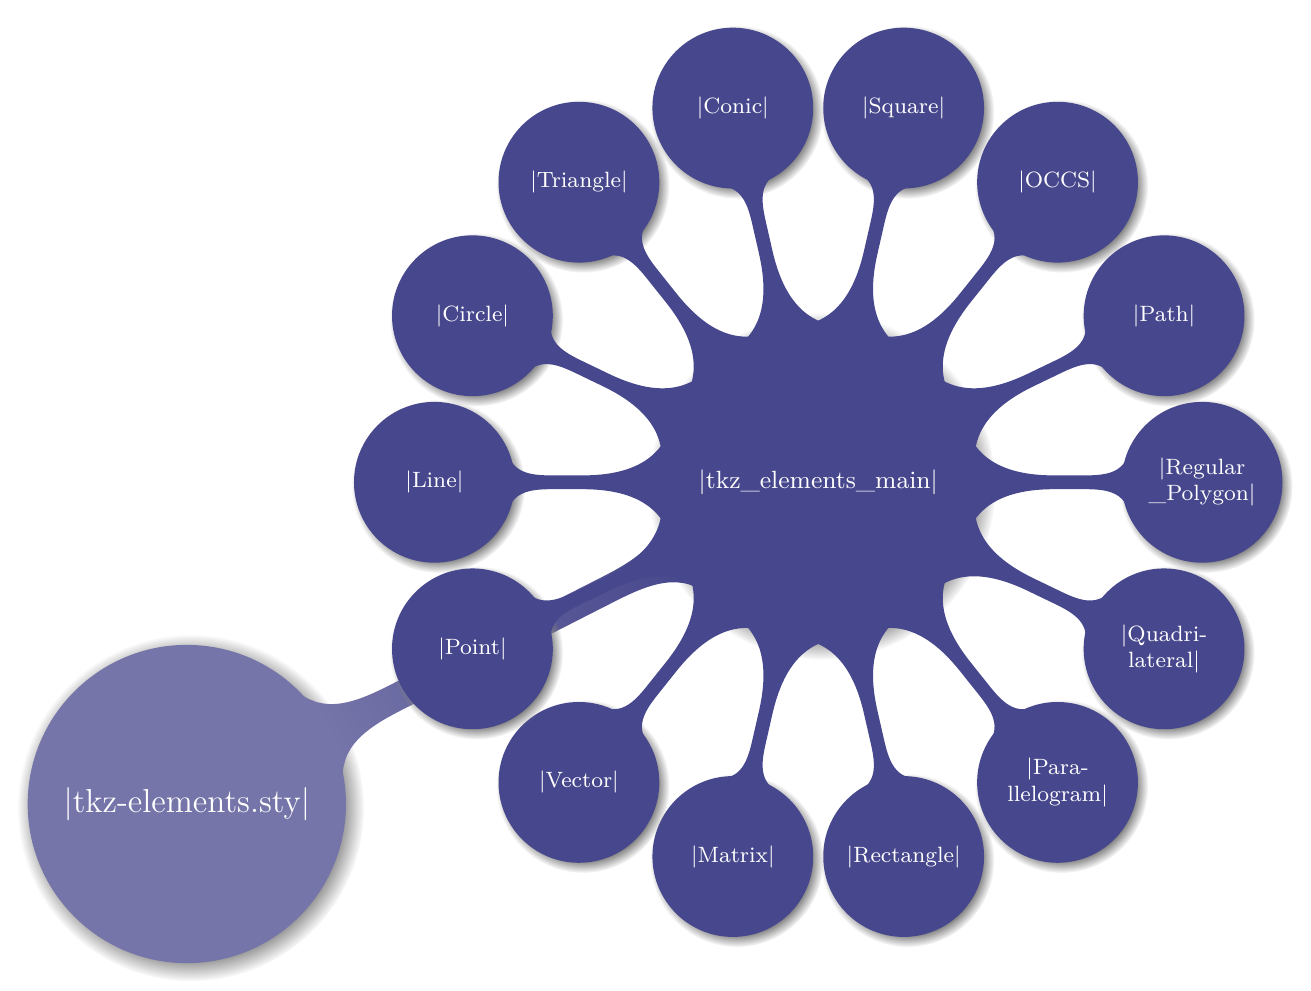
\begin{tikzpicture}[scale=.75]
\begin{scope}
\path[mindmap, concept color=MidnightBlue!60, text=white,text width=38mm,
 level 1 concept/.append style={level distance=120mm,
  sibling angle=72},
 set angles for level/.style={level 2/.append style={
 sibling angle=360/\the\tikznumberofchildren}},
 level/.append style={set angles for level=2},
 level 3 concept/.append style={level distance=20mm,
  sibling angle=20},
 L1/.style={level distance=45mm},
 L2/.style={level distance=65mm,minimum size=2cm}]

node[concept,circular drop shadow] {|tkz-elements.sty|} [clockwise from=10]

child[concept color= MidnightBlue!80,minimum size=4cm,text width=38mm,
clockwise from=27] {
  node[concept,circular drop shadow] {|tkz\_elements\_main|}
  [clockwise from=0]
  child[L2] { node[concept,circular drop shadow] {|Regular \_Polygon|} }
  child[L2] { node[concept,circular drop shadow] {|Quadri\-lateral|} }
  child[L2] { node[concept,circular drop shadow] {|Para\-llelogram|} }
  child[L2] { node[concept,circular drop shadow] {|Rectangle|} }
  child[L2] { node[concept,circular drop shadow] {|Matrix|} }
  child[L2] { node[concept,circular drop shadow] {|Vector|} }
  child[L2] { node[concept,circular drop shadow] {|Point|} }
  child[L2] { node[concept,circular drop shadow] {|Line|} }
  child[L2] { node[concept,circular drop shadow] {|Circle|} }
  child[L2] { node[concept,circular drop shadow] {|Triangle|} }
  child[L2] { node[concept,circular drop shadow] {|Conic|} }
  child[L2] { node[concept,circular drop shadow] {|Square|} }
  child[L2] { node[concept,circular drop shadow] {|OCCS|} }
  child[L2] { node[concept,circular drop shadow] {|Path|} }
};
\end{scope}
\end{tikzpicture}

目前的类有：

 \tkzClass{point} (z)、\tkzClass{circle} (C)、\tkzClass{line} (L)、\tkzClass{matrix} (M)、\tkzClass{occs} (O)、\tkzClass{parallelogram} (P)、\tkzClass{quadrilateral} (Q)、\tkzClass{rectangle} (R)、\tkzClass{square} (S)、\tkzClass{triangle} (T)、\tkzClass{vector} (V)、\tkzClass{conic} (CO)、\tkzClass{regular\_polygon} (RP) 和 \tkzClass{path} (PA)。\\

 括号中的变量表示通常赋予该类对象所在表的名称。

若 \tkzname{name} 指代某个类，则它的定义可在文件 \code{tkz\_elements\_name.lua} 中找到。
\endinput

\newpage
\section{为什么需要 tkz-elements？}

创建 \tkzNamePack{tkz-elements} 宏包，是为了解决在 TeX 中进行几何工作时的两个关键难题。第一，单靠 TeX 缺乏复杂几何计算所需的数值精度与灵活性。借助 \tkzname{Lua}，\tkzNamePack{tkz-elements} 为求交、投影、变换等运算提供了精确而稳定的计算。

第二，本宏包引入了面向对象的几何方法。点、向量、直线、圆、圆锥曲线等几何实体，都被建模为带有相关方法的结构化对象。这使得用户能够以更自然、更易读的方式来表达几何关系，贴近数学语言。

除了这两个核心思想之外，\tkzNamePack{tkz-elements} 还带来了以下几项额外的好处：

\begin{itemize}

 \item 简化计算：\tkzname{Lua} 的浮点运算与富有表现力的语法，使几何计算比在纯 TeX 中更易于书写和理解。

\item  可扩展性：得益于模块化设计和类的使用，新增几何对象与方法几乎毫不费力，使本宏包可扩展、可适应。

\item  互操作性：计算得到的点和数据能与 \TIKZ{} 或其他 TeX 绘图工具顺畅集成，让用户能够把计算与可视化有效地结合起来。

 \item 教学上的清晰：凭借其结构化且富有表现力的语法，\tkzNamePack{tkz-elements} 非常适合教学用途——在教学中，作图与记号的清晰性至关重要。
\end{itemize}

总而言之，\tkzNamePack{tkz-elements} 在 TeX 生态中提供了一个现代化的、面向对象的、由 Lua 驱动的几何作图框架。

\subsection{计算精度}
\subsubsection{\TIKZ{} 中的计算精度}
在 \TIKZ{} 中，表达式 \tkzimp{|veclen(x,y)|} 会计算 $\sqrt{x^2+y^2}$。
这一计算通过多项式逼近来实现，其思路借鉴了 \tkzimp{Rouben Rostamian} 的想法。

\pgfkeys{/pgf/number format/.cd,std,precision=5} \pgfmathparse{veclen(65,72)}
\begin{mybox}{}
\begin{verbatim}
   pgfmathparse{veclen(65,72)} \pgfmathresult
\end{verbatim}
\end{mybox}

 \tkzHand $\sqrt{65^2+72^2} \approx \pmpn{\pgfmathresult} $ 。

\subsubsection{Lua 中的计算精度}
可以如下定义一个 |luaveclen| 宏：

\begin{mybox}{}
\begin{verbatim}
\def\luaveclen#1#2{\directlua{tex.print(string.format(
'\percentchar.5f',math.sqrt((#1)*(#1)+(#2)*(#2))))}}
\end{verbatim}
\end{mybox}

以及

\begin{mybox}
\begin{verbatim}
\luaveclen{65}{72}
\end{verbatim}
\end{mybox}

得到：\tkzHand $\sqrt{65^2+72^2} = \pmpn{\luaveclen{65}{72}} $ {\color{red}！！}

\medskip
这个误差虽然在以百分之一磅为单位放置页面上的对象时微不足道，但对数学证明的结果来说却会成为问题。此外，这些不精确还会累积，并导致错误的作图。

\vspace{.5em}
为了解决这种精度不足的问题，我最初引入了 \tkzNamePack{fp}，随后又引入了 \tkzNamePack{xfp} 宏包。近来，随着 Lua\LATEX{} 的出现，我加入了一个 \tkzname{Lua} 选项，旨在用 \tkzname{Lua} 进行计算。

这是我创建这个宏包的主要动机，其次要目标是引入面向对象编程（OOP）并简化用 Lua 进行编程的方式。OOP 的概念促使我进一步探索它的各种可能性。

当时，我从 {\tkzimpbf{Nicolas Kisselhoff}} 那里收到了一些 Lua 编程示例，但起初我很难理解这些代码，于是我花时间耐心地学习 Lua。最终，我得以开发出 \tkzname{\tkznameofpack}，并融入了他的许多思想，我把它们改造后用于这个宏包。

\subsubsection{使用对象}
后来，我看到了 \tkzimp{Roberto Giacomelli}\footnote{\href{https://www.guitex.org/home/images/meeting2012/slides/presentazione_giacomell_guitmeeting_2012.pdf}{Grafica ad oggetti con LuaTEX}} 的一篇文章，内容是用 \tkzname{Lua} 和 \tkzNamePack{\TIKZ} 工具进行面向对象编程。这成为我灵感的第二个来源。这种方法不仅使编程可以一步一步地执行，而且对象的引入还在代码与几何之间建立了直接联系。结果，代码变得更加可读、明确，结构也更加良好。


\subsubsection{示例：阿波罗尼斯圆（新版本 2025/05/12）}
\label{ssub:example_apollonius_circle}

\begin{mybox}{问题：}
目标是找出一个与三角形的三个旁切圆都内切的圆。\end{mybox}


如需更多信息，可查阅 \href{https://mathworld.wolfram.com/ApolloniusCircle.html}{MathWorld} 上的相应条目。这个示例曾被用来测试 \tkzNamePack{tkz-euclide} 宏包。最初，用基本方法和现有工具得到的结果缺乏精度。得益于 \tkzNamePack{tkz-elements}，现在有了更强大、更精确的工具——而且它们也更易于使用。用 \tkzNamePack{tkz-euclide} 作图的核心原则保持不变：定义、计算、绘图和标注，都遵循一步一步的流程，与经典的尺规作图相呼应。这个版本利用了由 \tkzname{Lua} 所支持的最简便的作图方法。


\begin{mybox}
\begin{verbatim}
\directlua{
 init_elements()
 z.A = point(0, 0)
 z.B = point(6, 0)
 z.C = point(0.8, 4)
 T.ABC = triangle(z.A, z.B, z.C)
 z.N = T.ABC.eulercenter
 z.S = T.ABC.spiekercenter
 T.feuerbach = T.ABC:feuerbach()
 z.Ea, z.Eb, z.Ec = T.feuerbach:get()
 T.excentral = T.ABC:excentral()
 z.Ja, z.Jb, z.Jc = T.excentral:get()
 C.JaEa = circle(z.Ja, z.Ea)
% C.ortho = circle:radius(z.S, math.sqrt(C.JaEa:power(z.S)))
 C.ortho = C.JaEa:orthogonal_from(z.S) % 2025/05/12
 z.a = C.ortho.through
 C.euler = T.ABC:euler_circle()
 C.apo = C.ortho:inversion(C.euler)
 z.O = C.apo.center
 z.xa, z.xb, z.xc = C.ortho:inversion(z.Ea, z.Eb, z.Ec)}
\end{verbatim}
\end{mybox}

创建一个对象，就是定义它的属性和方法——也就是它的性质以及它所能执行的操作。对象一旦创建，就会通过存放在一个表中而与一个名字（或引用）相关联。这个表充当一个关联数组，把 \code{键}（引用）与 \code{值}（对象本身）联系起来。这些概念将在后面更详细地探讨。

例如，假设 \code{T} 是一个把三角形对象与键 \code{ABC} 关联起来的表。那么 \code{T.ABC} 就指向另一个包含该三角形属性的表——例如它的顶点、边或角——每个属性都通过一个特定的键来访问。这些属性在宏包内预定义好了，以支持几何运算。

\vspace{1em}
\begin{mybox}
\begin{verbatim}
 z.N = T.ABC.eulercenter
\end{verbatim}
\end{mybox}

\code{N} 是该点的名字，\code{eulercenter} 是三角形的一个属性。
\footnote{欧拉圆（即九点圆）的圆心，是每个三角形都具有的一个特征点。}

\begin{mybox}
\begin{verbatim}
 T.excentral = T.ABC:excentral()
\end{verbatim}
\end{mybox}

在这里，\tkzname{excentral} 是与 \tkzname{T.ABC} 对象相关联的一个方法。它定义了由三个旁切圆的圆心所构成的三角形。


\begin{tcolorbox}[
  title=已弃用代码,
  colframe=red!50,
  colback=red!5,
  coltitle=black,
  sharp corners,
  fonttitle=\bfseries,
  leftrule=1mm,
  rightrule=1mm,
  toprule=0.5mm,
  bottomrule=0.5mm
]
\texttt{注意：} 这段代码已被更优雅的版本取代。

有两行特别值得注意。第一行展示了 \tkzname{Lua} 卓越的精度如何使我们能够通过一次复杂的计算来定义半径。

根圆的半径由下式给出：
\[
\sqrt{\Pi(S,\mathcal{C}(Ja,Ea))}
\]
（即点 $S$ 关于以 |Ja| 为圆心、经过 |Ea| 的旁切圆的幂的平方根）。

\begin{mybox}{}
\begin{verbatim}
  C.ortho  = circle: radius (z.S,math.sqrt(C.JaEa: power(z.S)))
\end{verbatim}
\end{mybox}
\end{tcolorbox}

\begin{tcolorbox}[
  title=修订后的代码,
  colframe=cyan!60!black,
  colback=cyan!5,
  coltitle=white,
  sharp corners,
  fonttitle=\bfseries,
  leftrule=1mm,
  rightrule=1mm,
  toprule=0.5mm,
  bottomrule=0.5mm
]
\texttt{注意：} 以下代码以一种更优雅、更面向对象的方式取代了先前的版本。
先前的代码展示了可以手动执行的那类计算。然而，\tkzNamePack{tkz-elements} 为各种几何对象提供了丰富的方法。在与圆相关的方法中，有一个方法允许你在给定圆心的情况下，定义一个与另一个圆正交的圆。

我们希望得到一个与三角形三个旁切圆都正交的圆。它的圆心（$S$）就是这三个圆的根心。只需计算一个与其中之一正交的圆\footnote{给定一个主圆和两个辅圆，存在一个特定方法来定义与这三个圆都正交的根圆。}，以点 $S$ 为圆心即可。

第二行重要代码则是关于这个正交圆做一次反演。

\begin{mybox}{}
\begin{verbatim}
  C.ortho  = C.JaEa:orthogonal_from(z.S)
\end{verbatim}
\end{mybox}
\end{tcolorbox}

\vspace{1em}

最后，值得一提的是：把欧拉圆关于根圆做反演，就得到阿波罗尼斯圆。\footnote{九点圆，又称欧拉圆，与三个旁切圆都外切。切点构成费尔巴哈三角形。}

这个变换需要一个对象作为参数。该方法会自动检测对象类型（因为本宏包中所有对象都是有类型的），并据此选择合适的算法。

\begin{mybox}{}
\begin{verbatim}
  C.apo   = C.ortho:inversion(C.euler)
\end{verbatim}
\end{mybox}

现在所有相关的点都已定义好，接下来就该开始绘制几何路径了。为此，必须先创建相应的节点。这正是 \tkzMacro{tkz-elements}{tkzGetNodes} 宏的作用。

下一节专门讨论绘图，由 \tkzNamePack{tkz-euclide} 负责。

\begin{verbatim}
\begin{tikzpicture}
   \tkzGetNodes
   \tkzFillCircles[green!30](O,xa)
   \tkzFillCircles[teal!30](Ja,Ea Jb,Eb Jc,Ec)
   \tkzFillCircles[lightgray](S,a)
   \tkzFillCircles[green!30](N,Ea)
   \tkzDrawPoints(xa,xb,xc)
   \tkzDrawCircles(Ja,Ea Jb,Eb Jc,Ec S,a O,xa N,Ea)
   \tkzClipCircle(O,xa)
   \tkzDrawLines[add=3 and 3](A,B A,C B,C)
   \tkzDrawPoints(O,A,B,C,S,Ea,Eb,Ec,N)
   \tkzDrawSegments[dashed](S,xa S,xb S,xc)
   \tkzLabelPoints(O,N,A,B)
   \tkzLabelPoints[right](S,C)
\end{tikzpicture}
\end{verbatim}

\vspace{1em}
\directlua{
 init_elements()
 z.A = point(0, 0)
 z.B = point(6, 0)
 z.C = point(0.8, 4)
 T.ABC = triangle(z.A, z.B, z.C)
 z.N = T.ABC.eulercenter
 z.S = T.ABC.spiekercenter
 T.feuerbach = T.ABC:feuerbach()
 z.Ea, z.Eb, z.Ec = T.feuerbach:get()
 T.excentral = T.ABC:excentral()
 z.Ja, z.Jb, z.Jc = T.excentral:get()
 C.JaEa = circle(z.Ja, z.Ea)
 C.ortho = C.JaEa:orthogonal_from(z.S)
 z.a = C.ortho.through
 C.euler = T.ABC:euler_circle()
 C.apo = C.ortho:inversion(C.euler)
 z.O = C.apo.center
 z.xa, z.xb, z.xc = C.ortho:inversion(z.Ea, z.Eb, z.Ec)
}
\begin{minipage}{\textwidth}

\vspace{1em}
\begin{center}
\begin{tikzpicture}[ scale  = .6]
   \tkzGetNodes
   \tkzFillCircles[purple!50](O,xa)
   \tkzFillCircles[orange!50](Ja,Ea Jb,Eb Jc,Ec)
   \tkzFillCircles[yellow](S,a)
   \tkzFillCircles[purple!30](N,Ea)
   \tkzDrawPoints(xa,xb,xc)
   \tkzDrawCircles(Ja,Ea Jb,Eb Jc,Ec S,a O,xa N,Ea)
   \tkzClipCircle(O,xa)
   \tkzDrawLines[add=3 and 3](A,B A,C B,C)
   \tkzDrawPoints[red](O,A,B,C,S,Ea,Eb,Ec,N)
   \tkzDrawSegments[dashed](S,xa S,xb S,xc)
   \tkzLabelPoints(O,N,A,B)
   \tkzLabelPoints[right](S,C)
\end{tikzpicture}
\end{center}
\end{minipage}


\endinput

\newpage
\section{简介}
\subsection{几何构造理念}
\tkzNamePack{tkz-elements} 围绕经典欧几里得几何的原则而构建，强调只用无刻度直尺和圆规即可完成的作图。与代数或数值定义相比，本库更偏好声明式、几何化的方式。

这一理念意味着，所有几何对象——点、直线、圆、三角形等等——主要由其他点来定义。诸如坐标、距离或角度等显式数值会被刻意避免，除非它们对作图必不可少。这符合传统的尺规作图思维：几何推理来自可视化的构型，而不是来自数字。

例如：
\begin{itemize}
  \item 圆由其圆心和圆周上一点确定，
  \item 垂直平分线（中垂线）利用中点和对称性来构造，
  \item 角由三个点确定，而不是直接给出一个数值。
\end{itemize}

这一设计决策也解释了为什么基于标量值的构造器（例如 OCCS，即"一个圆心加一个标量"）不在默认接口之中。使用它们会引入数值依赖，与预期的几何抽象相悖。

\bigskip
尽管 \tkzNamePack{tkz-elements} 推崇一种高层的、基于点的几何方法，但它在内部依赖 \textbf{Lua} 来完成所有必要的计算。Lua 并不作为一种脚本工具暴露给用户，而是充当一个强大的计算引擎，在幕后实现精确而稳健的几何运算。

这种关注点分离让用户可以完全专注于几何构造，同时又能受益于 Lua 的计算精度和性能。下一节将说明，在本宏包的语境下 Lua 如何与 \LaTeX 结合——它不是作为一个编程层，而是作为一个不可见的伙伴，支撑起高级的几何构造。


\subsection{与 Lua 配合}
\tkzNamePack{tkz-elements} 的主要目的是执行几何计算，并用 \tkzname{Lua} 来定义点。你可以把它看作一个计算内核，既可由 \tkzNamePack{tkz-euclide} 使用，也可直接与 \tkzNamePack{\TIKZ} 配合使用。

\tkzname{Lua} 代码有两种执行方式：直接使用 \tkzMacro{lualatex}{directlua} 原语，或在 \tkzNamePack{luacode} 宏包（须单独加载）提供的 \tkzEnv{luacode}{luacode} 环境中执行。原先的 \texttt{tkzelements} 环境已被移除。
使用 \tkzMacro{lualatex}{directlua} 时，尤其是在复杂文档中，你可以用 \tkzFct{tkz-elements}{init\_elements()} 函数来重置内部数据结构——例如坐标表和缩放因子。

\begin{minipage}[t]{.52\textwidth}\vspace{0pt}%
   要点如下：
   \begin{itemize}
      \item 源文件必须以 \tkzRHand\ {\color{red}\uline{ \color{black}UTF-8}} 编码保存。
      \item 必须使用 \tkzRHand\ {\color{red}\uline{ \color{black}Lua\LATEX{}}} 进行编译。
      \item 你需要加载 \tkzNamePack{tkz-euclide} 和 \code{tkz-elements}。
      \item 所有定义和计算都在一个 \tkzClass{occs}（正交笛卡尔坐标系）中进行，既可通过 \tkzMacro{lualatex}{directlua} 宏使用 Lua，也可在 \tkzEnv{tkz-elements}{tkzelements} 环境中使用。
   \end{itemize}

右侧是一个最小模板。

代码主要分为两部分：Lua 代码（使用 \tkzMacro{lualatex}{directlua} 执行，或放在 \tkzEnv{luacode}{luacode} 环境中），以及 \tkzEnv{tikz}{tikzpicture} 环境——绘图命令（通常来自 \tkzNamePack{tkz-euclide}）就在此环境中发出。

使用 \tkzNamePack{tkz-euclide} 时，推荐使用 \code{mini} 选项，因为它只加载绘图所需的宏。
不过在目前阶段，某些绘图宏尚未完全独立于计算宏；
如果出现编译问题，干脆不加此选项直接加载 \tkzNamePack{tkz-euclide} 即可。

在 \tkzname{Lua} 部分中，最佳做法是始终调用
\tkzFct{tkz-elements}{init\_elements()} 函数。
该函数会重置内部表并清空内部数据结构。
\textbf{重要：} 从此时起，在 \tkzname{Lua} 代码中必须避免任何缩放操作。


\vspace*{4.1 cm}%
\end{minipage}\hspace*{\fill}
\begin{minipage}[t]{.45\textwidth}\vspace{0pt}%
\begin{mybox}
\begin{verbatim}
% !TEX TS-program = lualatex
% Created by Alain Matthes
\documentclass{standalone}
\usepackage[mini]{tkz-euclide}
% or simply TikZ
\usepackage{tkz-elements}
begin{document}

\directlua{
init_elements()
% definition of some points
z.A = point(   ,   )
z.B = point(   ,   )
% or
z.A = point:new(   ,   )
z.B = point:new(   ,   )

 ...code...
}

\begin{tikzpicture}
% points transfer to Nodes
% from Lua to tikz (tkz-euclide)
\tkzGetNodes

\end{tikzpicture}
\end{document}
\end{verbatim}
\end{mybox}
\end{minipage}

\subsection{主流程}

\tikzset{concept/.append style={fill={none}}}
\tikzset{root concept/.style=   {minimum size=3cm,text width=2.8cm}}%
\tikzset{level 1 concept/.append style={minimum size=4cm, font=\large, text width=3cm}}%

\begin{tikzpicture}
  \path[mindmap,concept color=orange,text=black]
    node[concept] {传递\\\textcolor{orange}{ \textbackslash{tkzGetNodes}}}
    child[concept color=red,grow=right] {
      node[concept] {绘图\\\textcolor{red}{tkz-euclide}\\\textcolor{red}{\TIKZ}} }
    child[concept color=purple,grow=left] {
    node[concept] {定义\\计算\\\textcolor{purple}{tkz-elements}} };
\end{tikzpicture}

取得绘图所需的全部点之后，必须把它们转换成 \tkzname{节点}，以便 \tkzNamePack{\TIKZ} 或 \tkzNamePack{tkz-euclide} 渲染图形。这通过宏 \tkzMacro{tkz-elements}{tkzGetNodes} 完成。该宏遍历表 \tkzname{z} 中的所有元素，使用键（本质上就是点的名字）并取回对应的值，即点（节点）的坐标。

\subsection{完整示例：帕普斯圆}
\label{sub:the_figure_pappus_circle}



\subsubsection{图形}

\directlua{
z.A = point(0, 0)
z.B = point(10, 0)
L.AB = line(z.A, z.B)
z.C = L.AB:gold_ratio()
L.AC = line(z.A, z.C)
L.CB = line(z.C, z.B)
L.AB = line(z.A, z.B)
z.O_0 = L.AB.mid
z.O_1 = L.AC.mid
z.O_2 = L.CB.mid
C.AB = circle(z.O_0, z.B)
C.AC = circle(z.O_1, z.C)
C.CB = circle(z.O_2, z.B)
z.P = C.CB.north
z.Q = C.AC.north
z.O = C.AB.south
z.c = z.C:north(2)
C.PC = circle(z.P, z.C)
C.QA = circle(z.Q, z.A)
z.P_0 = intersection(C.PC, C.AB)
z.P_1 = intersection(C.PC, C.AC)
_, z.P_2 = intersection(C.QA, C.CB)
T.P = triangle(z.P_0, z.P_1, z.P_2)
z.O_3 = T.P.circumcenter
}

\begin{center}
\begin{tikzpicture}[scale = .75]
 \tkzGetNodes
 \tkzDrawCircle[black,fill=yellow!20,opacity=.4](O_0,B)
 \tkzDrawCircles[teal,fill=teal!40,opacity=.6](O_1,C O_2,B)
 \tkzDrawCircle[purple,fill=purple!20,opacity=.4](O_3,P_0)
 \tkzDrawArc[cyan,delta=10](Q,A)(P_0)
 \tkzDrawArc[cyan,delta=10](P,P_0)(B)
 \tkzDrawArc[cyan,delta=10](O,B)(A)
 \tkzDrawPoints(A,B,C,O_0,O_1,O_2,P,Q,P_0,P_0,P_1,P_2,O)
 \tkzLabelPoints(A,B,C,O_0,O_1,O_2,P,Q,P_0,P_0,P_1,P_2,O)
\end{tikzpicture}
\end{center}

\subsubsection{代码}
\label{ssub:the_code}

\begin{mybox}{}
\begin{verbatim}
% !TEX TS-program = lualatex
\documentclass{article}
\usepackage[mini]{tkz-euclide} % mini = only tracing function
\usepackage{tkz-elements}
\begin{document}

\directlua{
  init_elements()  % Clear tables
  z.A = point(0, 0)
  z.B = point(10, 0)  %  creation of two fixed points $A$ and $B$
  L.AB = line(z.A, z.B)
  z.C = L.AB:gold_ratio()       %  use of a method linked to “line”
  z.O_0 = line(z.A, z.B).mid % midpoint of segment with an attribute of “line”
  z.O_1 = line(z.A, z.C).mid %  objects are not stored and cannot be reused.
  z.O_2 = line(z.C, z.B).mid
  C.AB = circle(z.O_0, z.B)  %  new object “circle” stored and reused
  C.AC = circle(z.O_1, z.C)
  C.CB = circle(z.O_2, z.B)
  z.P = C.CB.north            %  “north” attribute of a circle
  z.Q = C.AC.north
  z.O = C.AB.south
  z.c = z.C:north(2)   %“north” method of a point (needs a parameter)
  C.PC = circle(z.P, z.C)
  C.QA = circle(z.Q, z.A)
  z.P_0 = intersection(C.PC,C.AB)   %  search for intersections of two circles.
  z.P_1 = intersection(C.PC,C.AC)   %   idem
  _,z.P_2 = intersection(C.QA,C.CB)   %  idem
  T.P = triangle(z.P_0, z.P_1, z.P_2)
  z.O_3 = T.P.circumcenter  % circumcenter attribute of “triangle”
}
\end{verbatim}
\end{mybox}

\begin{verbatim}
\begin{tikzpicture}
  \tkzGetNodes
  \tkzDrawCircle[black,fill=yellow!20,opacity=.4](O_0,B)
  \tkzDrawCircles[teal,fill=teal!40,opacity=.6](O_1,C O_2,B)
  \tkzDrawCircle[purple,fill=purple!20,opacity=.4](O_3,P_0)
  \tkzDrawArc[cyan,delta=10](Q,A)(P_0)
  \tkzDrawArc[cyan,delta=10](P,P_0)(B)
  \tkzDrawArc[cyan,delta=10](O,B)(A)
  \tkzDrawPoints(A,B,C,O_0,O_1,O_2,P,Q,P_0,P_0,P_1,P_2,O)
  \tkzLabelPoints(A,B,C,O_0,O_1,O_2,P,Q,P_0,P_0,P_1,P_2,O)
\end{tikzpicture}
\end{document}
\end{verbatim}

\subsection{另一个带注释的示例：南极点}
下面是另一个带注释的示例

\begin{mybox}{}
\begin{verbatim}
% !TEX TS-program = lualatex
\documentclass{standalone}
\usepackage[mini]{tkz-euclide}
\usepackage{tkz-elements}
\begin{document}
\directlua{
 init_elements()                     % Clear tables
 z.A = point(2, 4)
 z.B = point(0, 0)                   % three fixed points are used
 z.C = point(8, 0)                   %
 T.ABC = triangle(z.A, z.B, z.C)     % we create a new triangle object
 C.ins = T.ABC:in_circle()           % we get the incircle of this triangle
 z.I = C.ins.center                  % center is an attribute of the circle
 z.T = C.ins.through                 % through is also an attribute
 z.I, z.T = C.ins:get()              % get() is a shortcut
 C.cir = T.ABC:circum_circle()       % we get the  circumscribed circle
 z.W = C.cir.center                  % we get the center of this circle
 z.O = C.cir.south                   % now we get the south pole of this circle
 L.AO = line(z.A, z.O)               % we create an object "line"
 L.BC = T.ABC.bc                     % we get the line (BC)
 z.I_A = intersection(L.AO, L.BC)    % we search the intersection of the last lines
}
\end{verbatim}
\end{mybox}

\directlua{
 init_elements()
 z.A = point(2, 4)
 z.B = point(0, 0)
 z.C = point(8, 0)
 T.ABC = triangle(z.A, z.B, z.C)
 C.ins = T.ABC:in_circle()
 z.I = C.ins.center
 z.T = C.ins.through
 C.cir = T.ABC:circum_circle()
 z.W = C.cir.center
 z.O = C.cir.south
 L.AO = line(z.A, z.O)
 L.BC = T.ABC.bc
 z.I_A = intersection(L.AO, L.BC)
}

\begin{center}
  \begin{tikzpicture}[ scale= 1.2]
  \tkzGetNodes
  \tkzDrawCircles(W,A I,T)
  \tkzDrawArc(O,C)(B)
  \tkzDrawPolygon(A,B,C)
  \tkzDrawSegments[new](A,O B,O C,O)
  \tkzDrawLine(B,I)
  \tkzDrawPoints(A,B,C,I,I_A,W,O)
  \tkzFillAngles[green!20,opacity=.3](A,O,B A,C,B)
  \tkzFillAngles[teal!20,opacity=.3](O,B,C B,C,O B,A,O O,A,C)
  \tkzLabelPoints(I,I_A,W,B,C,O)
  \tkzLabelPoints[above](A)
  \end{tikzpicture}
\end{center}

\vspace{12pt}
下面是用于出图的 \tkzEnv{tikz}{tikzpicture} 环境：
\begin{verbatim}
\begin{tikzpicture}
\tkzGetNodes
\tkzDrawCircles(W,A I,T)
\tkzDrawArc(O,C)(B)
\tkzDrawPolygon(A,B,C)
\tkzDrawSegments[new](A,O B,O C,O)
\tkzDrawLine(B,I)
\tkzDrawPoints(A,B,C,I,I_A,W,O)
\tkzFillAngles[green!20,opacity=.3](A,O,B A,C,B)
\tkzFillAngles[teal!20,opacity=.3](O,B,C B,C,O B,A,O O,A,C)
\tkzLabelPoints(I,I_A,W,B,C,O)
\tkzLabelPoints[above](A)
\end{tikzpicture}
\end{verbatim}
\endinput
\newpage

\section{书写约定、最佳实践与常见错误}
\subsection{给对象命名}

\textbf{注意：} 某些变量（如 \tkzname{z}、\tkzname{L}、\tkzname{T} 等）是为存储几何对象而保留的。
重新给其中之一赋值（例如 \tkzname{L = 4}）会覆盖其内容并破坏系统。

点是一种特殊情况：点必须存放在表 \tkzname{z} 中。
对于所有其他几何对象，强烈建议遵循预定义的变量名。
避免混用命名约定或自行发明标识符，否则可能导致不可预知的行为。

\vspace{1em}
\tkzRHand{\textcolor{red}{警告}}：不要把 \texttt{point}、\texttt{line}、\texttt{circle}、\texttt{path}、\texttt{triangle} 等名字复用为变量名。
这些标识符由 \tkzNamePack{tkz-elements} 在内部保留，用于表示对象构造器。

\vspace{1em}
下面列出保留的类以及与之对应的默认变量名：
\label{list of reserved classes}

\vspace{1em}
\textcolor{red}{\directlua{
  for _, t in ipairs(tkz.tables) do
    local class = (string.gsub(t[2], "_", "\\_"))
    tex.sprint(class .. "  -->  " .. t[1] .. "\\\\")
  end
} }

\subsection{最佳实践}

最好使用方法——更好的是使用对象属性——而不是独立函数。

例如，要确定线段 $AB$ 的中点，以前可以这样写：

|z.m = midpoint(z.A, z.B)|。现在这被认为是不正确的：你必须使用

|z.m = tkz.midpoint(z.A, z.B)|。

不过，推荐的做法是先用下面的语句定义线段：

|L.AB = line(z.A, z.B)|，然后使用属性：

|z.m = L.AB.mid|。如果你不复用这条直线，那么写成一行 |z.m = line(z.A, z.B).mid| 也是可以接受的。

\vspace{12pt}
类似地，过去可能有人想写 |L.bi = tkz.bisector(z.A, z.B, z.C)| 来求顶点 $A$ 处的角平分线。和上一个例子一样，现在这不再有效。你现在必须使用：

|L.bi = tkz.bisector(z.A, z.B, z.C)|，因为所有独立函数都已归到 |tkz| 模块之下。

更好的做法是先用下面的语句定义三角形 $ABC$：

|T.ABC = triangle(z.A, z.B, z.C)|，然后通过下面的方式访问角平分线：

|L.bi = T.ABC:bisector(z.A)|，或直接：

|L.bi = triangle(z.A, z.B, z.C):bisector(z.A)|。

\subsection{常见错误与最佳实践}

\vspace{1em}
\tkzRHand{\textcolor{red}{第二个警告}}：我们来看看错误赋值的后果。下面这个例子很简单：定义两个点、过这两点的直线，以及在其中一点处与第一条直线正交的直线。为定义这些对象，我们使用两个表（即类）：\tkzname{z} 和 \tkzname{L}。

下面是正确的代码：
\begin{mybox}{}
\begin{tkzexample}[latex=.5\textwidth]
\directlua{
  z.A = point(1, 2)
  z.B = point(3, -1)
  L.AB = line(z.A, z.B)
  -- blunders
  L.ortho = L.AB:ortho_from(z.B)
  z.C = L.ortho.pb
}
\begin{tikzpicture}[scale = .75]
  \tkzGetNodes
  \tkzDrawLines(A,B B,C)
  \tkzDrawPoints(A,B)
\end{tikzpicture}
\end{tkzexample}
\end{mybox}

\begin{itemize}
  \item \textbf{第一个错误：} \tkzname{z = nil} 或 \tkzname{z = 4}。你重新赋值了 \tkzname{z} 变量。它不再指向一个表，而是指向一个数字。它的类型变了，系统再也无法访问这些点。
  \item \tkzname{z.A = 4} 同样有问题：你覆盖了点 $A$。如果你想移除点 $A$，那就应该改用 \tkzname{z.A = nil}。
  \item \tkzname{L = 4}。用它来存一个长度看似方便，但这样做会擦掉整张直线表。
  \item \tkzname{L.ortho = ortho}。一个更隐蔽的错误：如果 \tkzname{ortho} 没有定义，你就丢失了这条直线。如果它已定义但类型不对，则会报错。
  \item 对于点以外的对象，在流程末尾进行错误赋值可能不会影响图形。可以在绘图之前清理表。不过，\tkzname{z} 表绝不能被改动。只应删除那些未用于绘图的点。
\end{itemize}

这些预防措施有助于保证系统的一致性，防止不可预知的行为。

\vspace{1em}
下面我们说明如何为每一类对象指定变量名。


\subsection{给点命名}

如果你打算稍后在 \tkzNamePack{\TIKZ} 或 \tkzNamePack{tkz-euclide} 中使用点，就必须把它们存放在表 \tkzname{z} 中。
在 \tkzNamePack{tkz-elements} 中，所有点都遵循 \tkzname{z.name} 的约定，其中 \tkzname{name} 就是希望使用的节点标签。

\medskip
当使用 \tkzcname{tkzGetNodes} 把点传递给 \TIKZ{} 时，
每个条目 \code{z.name} 都会生成对应的坐标：

\begin{mybox}
\verb|\coordinate (name) at (x,y);|
\end{mybox}

有些命名情况需要留意，特别是涉及撇号（prime）的情况。

\paragraph{撇号记号。}

宏 \tkzcname{tkzGetNodes} 会把 Lua 名字中的某些结尾模式
转换成 \TIKZ{} 中的单撇号或双撇号记号。

\begin{itemize}
  \item 以 \code{p} 结尾的名字变成单撇号：
        \begin{mybox}
        \verb|z.Bp = point(...)|  →  节点 \verb|(B')|
        \end{mybox}

  \item 以 \code{pp} 结尾的名字变成双撇号：
        \begin{mybox}
        \verb|z.Bpp = point(...)| → 节点 \verb|(B'')|
        \end{mybox}
\end{itemize}

这一约定对几何作图很方便，但如果结尾的 \code{p} 或 \code{pp} 并非有意表示撇号，就可能导致意外的重命名。

\begin{tcolorbox}[colback=red!7,colframe=red!60!black,title=警告]
避免使用以 \code{p} 或 \code{pp} 结尾的名字，除非你确实想在 \TIKZ{} 中使用单撇号或双撇号记号。
\end{tcolorbox}

\medskip
 你可以在 \code{lua} 部分随意使用这些名字，但在用 \verb|\tkzGetNodes| 宏把点传递成节点时会出错。为避免错误，请使用下一段给出的办法之一。对于 \code{z.p}，只要改用 \code{z.P} 即可。小写字母可以在 \TIKZ{} 中取回。

\paragraph{中间名字。}

为便于阅读，或在 Lua 中使用较长或描述性的名字时，
你可以使用一个中间变量，并可选地为绘图指定一个简短标签。

例如：

\begin{mybox}
\verb|local euler = point(...)|
\verb|z.E = euler|
\end{mybox}

这里，这个点在内部以清晰的名字 \code{euler} 存放，
但在 \TIKZ{} 中显示为节点 \code{(E)}。

如果你希望在 Lua 和 \TIKZ{} 中都保留长名字，直接写：

\begin{mybox}
\verb|z.euler = point(...)|
\end{mybox}

或者，你也可以在 \TIKZ{} 层指定一个别名：

\begin{mybox}
\verb|\pgfnodealias{E}{euler}|
\end{mybox}

另一种可行做法是：在传递之前，先用一个可接受的名字（例如 \code{A}），再用 \verb|z.apollonius = nil| 删除点 \code{z.apollonius}。

\begin{mybox}
\verb|z.A = z.apollonius|
\verb|z.apollonius = nil|
\end{mybox}



\paragraph{合法示例。}\mbox{}

\begin{mybox}
\begin{itemize}
  \item \verb|z.A = point(1,2)|     → 节点 \verb|(A)|
  \item \verb|z.Bp = point(3,4)|     → 节点 \verb|(B')|
  \item \verb|z.Cpp = point(5,1)|    → 节点 \verb|(C'')|
  \item \verb|z.H_a = T.ABC:altitude()| → 节点 \verb|(H_a)|
  \item \verb|z.euler = T.ABC.eulercenter| → 节点 \verb|(euler)|
\end{itemize}
\end{mybox}

名字可以包含字母、数字和“\_”。
其他字符应避免使用，因为它们可能无法构成合法的 TikZ
节点名。

\paragraph{Lua 提示。}

表 \tkzname{z} 的字段可以这样访问：

\begin{itemize}
  \item \verb|z.A|（语法糖），或
  \item \verb|z["A"]|
\end{itemize}

把 \verb|z.A = nil| 会彻底删除该点。


\subsection{给其他对象命名}
对于点以外的所有几何对象，你可以自由选择名字。不过，采用一致的命名约定能大大提高代码的可读性和可维护性。更确切地说，每个 Lua 代码块之前通常会调用 \tkzFct{tkz-elements}{init\_elements()} 函数，其作用是清空并重置各个表（如 \tkzname{L}、\tkzname{C} 等）。如果你选择使用自定义的变量名或结构，那完全可以——但那样一来，你就需要自己负责手动管理和清理变量与表，以避免冲突或意外行为。

本文档采用如下命名策略：


对象存放在专门的表中，每个表对应一个特定的类。
这些表由如下变量表示：
\begin{itemize}

\item \tkzname{L} 用于直线和线段
\item \tkzname{C} 用于圆
\item \tkzname{T} 用于三角形
\item \tkzname{CO} 用于圆锥曲线（包括椭圆、双曲线和抛物线）

\item 等等。参见保留字列表 [\ref{list of reserved classes}]
\end{itemize}

下面是一些使用中的命名约定示例：

\begin{itemize}
  \item 直线（L）：\\
  名字反映确定该直线的两个点。

   示例：|L.AB = line(z.A, z.B)| -- 经过 A 和 B 的直线

\item 圆（C）\\
你可以根据定义点或用途来命名一个圆。
示例：
\begin{itemize}
 \item C.AB       --> 圆心在 A、过 B 的圆
 \item C.euler    --> 欧拉圆（九点圆）
 \item C.external --> 外部圆
\end{itemize}

\item 三角形（T）\\
使用顶点标签，或在合适时使用描述性名字。示例：

\begin{itemize}
  \item T.ABC         --> 顶点为 A、B、C 的三角形
  \item T.feuerbach   --> 费尔巴哈三角形

\end{itemize}



\item 圆锥曲线（CO）\\
表 CO 可以存放各种圆锥曲线；使用有意义的键来表明类型和作用。


\end{itemize}

注意：\emph{虽然你可以选择其他变量名或格式，但遵循这些约定能确保代码清晰易读，尤其是在处理较复杂的图形时。}

\subsection{属性、方法的书写约定。}
\label{sub:writing_conventions_for_attributes_methods_and_functions}

访问属性或调用方法时，必须遵循标准的 Lua 约定：

\begin{itemize}
  \item \textbf{属性} 用点记号访问：\verb|object.attribute|。
    \begin{itemize}
      \item 例如，要访问点 \verb|A| 的坐标，用 \verb|z.A.re| 表示横坐标，用 \verb|z.A.im| 表示纵坐标。
      \item 要得到对象的类型，写 \verb|z.A.type|。
      \item 要取圆 \verb|C.OA| 的南极点，写 \verb|C.OA.south|。
    \end{itemize}

  \item \textbf{方法} 用冒号记号调用：\verb|object:method()|。
    \begin{itemize}
      \item 例如，要计算三角形 \verb|ABC| 的内切圆，使用：\verb|C.incircle = T.ABC:in_circle()|。
      \item 如果方法需要参数，就放在括号里。例如，要计算点 \verb|C| 到直线 \verb|(AB)| 的距离：\verb|d = L.AB:distance(z.C)|。
    \end{itemize}

  \item \textbf{丢弃结果}：如果一个函数返回多个值而你只需要其中一个，用 \verb|_| 忽略其余的。
    \begin{itemize}
      \item 例如，只想取直线与圆的第二个交点：

      \verb|_, z.J = intersection(L.AB, C.OC)|。
    \end{itemize}
\end{itemize}

\subsection{其他事项}
\label{sub:miscellanous}
\begin{itemize}
  \item \texttt{单位与坐标：} 与 \tkzNamePack{tkz-euclide} 一样，默认单位是厘米。所有点都放在一个正交笛卡尔坐标系中。

  \item \texttt{数值变量：} 实数遵循标准的 Lua 记法约定。

  \item \texttt{复数：} 与实数类似，但必须用 point 构造器来定义。例如：
  \begin{verbatim}
  za = point(1, 2)
  \end{verbatim}
  这在数学上对应于 \(1 + 2i\)。你可以用下面的语句打印该复数：
  \begin{verbatim}
  tex.print(tostring(za))
  \end{verbatim}

  \item \texttt{布尔值：}
  \begin{itemize}
    \item 在 Lua 中：\verb|bool = true| 或 \verb|bool = false|
    \item 你可以使用下面的 \tkzname{Lua} 代码：
    \begin{verbatim}
    if bool == true then ... else ... end
    \end{verbatim}
    \item 在 LaTeX 中，加载 \tkzNamePack{ifthen} 宏包后，你可以写：
    \begin{verbatim}
    \ifthenelse{\equal{\tkzUseLua{bool}}{true}}{<true code>}{<false code>}
    \end{verbatim}
  \end{itemize}

  \item \texttt{字符串：}
  \begin{itemize}
    \item Lua 示例：\verb|st = "Euler's formula"|
    \item 在 LaTeX 中：\verb|\tkzUseLua{st}| 将显示 \texttt{Euler's formula}
  \end{itemize}
\end{itemize}
\endinput
\section{工作组织}
\label{sec:work_organization}


下面给出使用 \tkzNamePack{tkz-euclide} 与 \tkzEngine{Lua\LATEX} 时的一种示例组织方式。

\begin{itemize}
  \item \texttt{编译方式：} 添加如下一行：
  \begin{verbatim}
  % !TEX TS-program = lualatex
  \end{verbatim}
  以确保文档使用 \tkzEngine{Lua\LATEX} 编译。

  \item \texttt{文档类：} 如果目的只是绘制一幅图形，推荐使用 \texttt{standalone} 文档类，因为它可避免不必要的开销。

  \item \texttt{宏包加载：} 你可以用两种方式加载 \tkzNamePack{tkz-euclide}：
  \begin{itemize}
    \item \tkzcname{usepackage\{tkz-euclide\} } 让你获得整个宏包的完整功能。
    \item 推荐的做法是使用 \tkzPopt{tkz-euclide}{mini} 选项，它只加载绘图所需的模块。如果你愿意，仍然可以直接用 \TIKZ{} 绘图。
  \end{itemize}

  \item \texttt{条件判断：} 当你需要在文档中求值布尔条件时，\tkzNamePack{ifthen} 宏包很有用。

  \item \texttt{Lua 代码组织：} 虽然你可以直接用 \verb|\directlua| 嵌入 Lua 代码，但把代码外置有如下几个好处：
  \begin{itemize}
    \item 在支持 \tkzname{Lua} 和 \LATEX{} 的编辑器中，可以获得更好的语法高亮与代码展示效果。
    \item 注释更简单：\tkzname{Lua} 使用 \verb|--|，而 \LATEX{} 使用 \verb|%|。把 Lua 放在单独的文件里可避免混淆。
    \item 可复用：外部代码文件可在多个文档或图形之间复用。
  \end{itemize}
\end{itemize}

为简单起见，本文档在大多数情况下使用内嵌的 Lua 代码。不过在某些示例中，会使用外部文件来向你展示具体做法。


\vspace{12pt}
\begin{mybox}{}
\begin{minipage}{.50\textwidth}
\begin{verbatim}
% !TEX TS-program = lualatex
% Created by Alain Matthes on 2024-01-09.
\documentclass[margin = 12pt]{standalone}
\usepackage[mini]{tkz-euclide}
\usepackage{tkz-elements,ifthen}

\begin{document}
\directlua{
 init_elements() % Clear tables
 dofile ("lua/sangaku.lua")
 % Load the lua code
}
\begin{tikzpicture}[ scale = .75]
 \tkzGetNodes
 \tkzDrawCircle(I,F)
 \tkzFillPolygon[purple](A,C,D)
 \tkzFillPolygon[blue!50!black](A,B,C)
 \tkzFillCircle[orange](I,F)
\end{tikzpicture}
\end{document}
\end{verbatim}
\end{minipage}
\begin{minipage}{.40\textwidth}
\directlua{
 init_elements()
 dofile ("lua/sangaku.lua")
}
\begin{center}
\begin{tikzpicture}[ scale = .75]
  \tkzGetNodes
  \tkzDrawCircle(I,F)
  \tkzFillPolygon[purple](A,C,D)
  \tkzFillPolygon[blue!50!black](A,B,C)
  \tkzFillCircle[orange](I,F)
\end{tikzpicture}
\end{center}
\end{minipage}
\end{mybox}

\vspace{12pt}
下面是 \tkzname{Lua} 部分的代码：文件 |sangaku.lua|

\vspace{1em}
\begin{minipage}{.5\textwidth}
\begin{mybox}
\begin{verbatim}
 z.A = point(0, 0)
 z.B = point(8, 0)
 L.AB = line(z.A, z.B)
 S.AB = L.AB:square()
 _, _, z.C, z.D = S.AB:get()
 z.F = S.AB.ac:projection(z.B)
 L.BF = line(z.B, z.F)
 T.ABC = triangle(z.A, z.B, z.C)
 L.bi = T.ABC:bisector(2)
 z.c = L.bi.pb
 L.Cc = line(z.C, z.c)
 z.I = intersection(L.Cc, L.BF)
\end{verbatim}
\end{mybox}
\end{minipage}


\subsection{缩放策略的更新}

在以前的版本中，建议在代码的 Lua 部分进行缩放。不过，这一指导原则现在已经改变。

由于所有几何计算都在 \tkzname{Lua} 中完成，在 \TIKZ{} 中进行缩放已不再有任何问题。相反，在 \tkzname{Lua} 中进行缩放却带来了若干麻烦——尤其是最近实现的与圆锥曲线相关的函数，它们涉及大量使用实数的距离计算。

这些问题促使我们重新审视了若干函数，并在此过程中发现并修复了一些与 Lua 端缩放相关的 bug。

\medskip

\textbf{\textcolor{red}{新的建议：}} 从现在起，缩放应只在 \TIKZ{} 部分进行。\tkzname{Lua} 代码应在一个未经缩放、一致的坐标系中运行，以确保所有几何计算的可靠性。

本文档后续只在 \tkzEnv{tikz}{tikzpicture} 环境中使用缩放。
\endinput
\newpage\section{坐标}

本节概述用户可用的各种坐标系。既然缩放操作已从 \tkzname{Lua} 层移除，这样的说明就显得比以往任何时候都更有必要。

\subsection{坐标的一般用法}
与 \tkzNamePack{tkz-euclide} 一样，\tkzNamePack{tkz-elements} 建立在二维正交笛卡尔坐标系之上，默认单位为厘米。

在一个专注于欧几里得几何的语境中使用我们将要介绍的 \emph{occs}（正交坐标系）会是不协调的。

此外，在 \tkzNamePack{tkz-elements} 中，点的概念与一个复数的附标绑定在一起。为保持代码清晰一致，在 Lua 内部修改单位的选项已被刻意省略。

\medskip

\textbf{结论：} 对于用 \tkzNamePack{tkz-elements} 创建的任何图形，所有点都放在一个以厘米为单位的二维正交坐标系中。

   \begin{tikzpicture}
   \pgfkeys{/pgf/number format/.cd,std,precision=2}
   \let\pmpn\pgfmathprintnumber
   \tkzDefPoints{2/3/M,0/0/O,2/0/A,0/3/B}
   \tkzLabelPoints(O)
   \tkzLabelPoint[right](M){$M: z_M = 2 + 3i$}
   \tkzDrawPoints(M,O)
   \tkzPointShowCoord(M)
   \tkzLabelPoint[below,teal](A){$2$}
   \tkzLabelPoint[left,teal](B){$3$}
   \tkzDrawSegments[->,add = 0 and 0.25](O,B O,A)
   \begin{scope}[every annotation/.style={fill=lightgray!15,anchor = east}]
   \node [annotation,font =\small,text width=6cm] at (current bounding box.west) {
$M$ 的坐标
   \begin{mybox}{}
   \code{ z.A = point(2, 3)}
   \end{mybox}
       };
   \end{scope}
   \end{tikzpicture}

\subsection{重心坐标的使用}

重心坐标描述一个点相对于参考三角形的位置。平面上任意一点都可以用重心坐标表示，这些坐标在相差一个标量倍数（位似）的意义下确定。或者，也可以把它们归一化，使三者之和等于 1。

重心坐标在三角形几何中特别有用，尤其是在分析那些在仿射变换下不变的性质——即不依赖于角度的性质——时。

考虑三角形 $ABC$。人们可以用重心坐标来定义重心、垂心等关键点。

\medskip
\texttt{关于垂心。}

计算垂心的重心坐标需要知道三角形的三个角。它们作为属性存放在表 \texttt{T.ABC} 中：
\begin{itemize}
  \item \texttt{T.ABC.alpha} —— 顶点 $A$ 处的角 $\widehat{A}$
  \item \texttt{T.ABC.beta}  —— 顶点 $B$ 处的角 $\widehat{B}$
  \item \texttt{T.ABC.gamma} —— 顶点 $C$ 处的角 $\widehat{C}$
\end{itemize}

见 [\ref{ssub:_triangle_barycentric_ka_kb_kc}]

\medskip
\texttt{取回重心坐标。}

可以计算一个给定点相对于某个三角形的重心坐标。返回的值会自动归一化。用法见第 [\ref{ssub:_triangle_barycentric__coordinates_pt}] 节。


\begin{minipage}{.5\textwidth}
\directlua{
z.A = point(0, 0)
z.B = point(3, 1)
z.C = point(1, 3)
T.ABC = triangle(z.A, z.B, z.C)
z.G = T.ABC:barycentric(1,1,1)
z.H = T.ABC:barycentric(math.tan(T.ABC.alpha),
                        math.tan(T.ABC.beta),
                        math.tan(T.ABC.gamma))}
\begin{tikzpicture}
\tkzGetNodes
\tkzDrawPolygon(A,B,C)
\tkzDrawPoints(A,B,C,G,H)
\tkzLabelPoints(A,B,G)
\tkzLabelPoints[above](C,H)
\end{tikzpicture}
\end{minipage}
\begin{minipage}{.5\textwidth}
\begin{tkzexample}[code only]
\directlua{
z.A = point(0, 0)
z.B = point(3, 1)
z.C = point(1, 3)
T.ABC = triangle(z.A, z.B, z.C)
z.G = T.ABC:barycentric(1, 1, 1)
z.H = T.ABC:barycentric(math.tan(T.ABC.alpha),
                        math.tan(T.ABC.beta),
                        math.tan(T.ABC.gamma))}
\end{tkzexample}
\end{minipage}

\subsection{三线坐标的使用}
\label{sub:use_of_trilinear_coordinates}

点 $P$ 相对于三角形 $ABC$ 的三线坐标，是一组与 $P$ 到三角形各边的有向距离成比例的三个数。这些坐标是齐次的，通常写作 $x : y : z$ 或 $(x, y, z)$。

由于只有坐标之间的比值才有意义，三线坐标特别适合表达那些在缩放不变的几何关系。

于是在下一个示例中有 $ a' : b' : c' = ka : kb : kc$（其中 $a = BC, b = AC, c = AB$）。

\begin{minipage}{.5\textwidth}
\directlua{
z.A = point(0, 0)
z.B = point(5, 0)
z.C = point(1, 3)
T.ABC = triangle(z.A, z.B, z.C)
z.L = T.ABC:trilinear(T.ABC.a,
                      T.ABC.b,
                      T.ABC.c)
z.a, z.b, z.c = T.ABC:projections(z.L)}
\begin{tikzpicture}
\tkzGetNodes
\tkzDrawPolygon(A,B,C)
\tkzDrawSegments(L,a L,b L,c)
\tkzDrawPoints(A,B,C,L)
\tkzLabelPoints(A,B)
\tkzLabelPoints[above](C,L)
\tkzLabelSegment[left](L,a){$ka$}
\tkzLabelSegment[above](L,b){$kb$}
\tkzLabelSegment[right](L,c){$kc$}
\end{tikzpicture}
\end{minipage}
\begin{minipage}{.5\textwidth}
\begin{tkzexample}[code only]
\directlua{
z.A = point(0, 0)
z.B = point(5, 0)
z.C = point(1, 3)
T.ABC = triangle(z.A, z.B, z.C)
z.L = T.ABC:trilinear(T.ABC.a,
                      T.ABC.b,
                      T.ABC.c)
z.a, z.b, z.c = T.ABC:projections(z.L)}
\end{tkzexample}
\end{minipage}

\subsection{OCCS}

该类的对象就是 \emph{正交笛卡尔坐标系}。它们由参考坐标系经过平移和旋转得到。可用于简化某些表达式和坐标。
见 [\ref{sec:orthonormal_cartesian_coordinate_system}
]
\endinput
%--------------------------------------------------------------------
\section{数值容差}
\label{sec:numerical_tolerance}

\subsection{浮点运算}

\tkzNamePack{tkz-elements} 中的所有计算均采用浮点运算完成。
因此，实数之间的精确比较并不可靠。

例如，一个理论上位于某条直线上的点，由于舍入误差，可能会产生一个非常小的非零值。

\subsection{全局容差：\code{tkz.epsilon}}

为保证数值稳健性，\tkzNamePack{tkz-elements}
使用了一个全局容差参数：


\verb|tkz.epsilon = 1e-10|


该值规定了几何判定（共线、关联、距离相等等）中允许的数值误差。

\medskip
默认情况下，该容差被设为一个较小的正值。
如有需要，高级用户可对其进行调整。

\subsection{在位置判定中的使用}

所有从属关系与位置判定均为 \emph{EPS 感知}。
当某个方法接受可选参数 \code{EPS} 时，遵循以下规则：

\begin{itemize}
\item 若提供了 \code{EPS}，则它会覆盖全局容差。
\item 否则使用 \code{tkz.epsilon}。
\end{itemize}

这一设计保证了所有几何对象之间的一致性。

%--------------------------------------------------------------------
\section{几何关系 API}
\label{sec:geometric_relations_api}

\subsection{一般原则}

在 \tkzNamePack{tkz-elements} 中，几何对象提供一个统一的方法
\[
\code{object:position(other\_object[, EPS])}
\]
用于判定几何关系。

判定结果取决于第二个参数（\code{other\_object}）的类型。

\medskip
所有位置判定均带有容差。
若未指定，可选参数 \code{EPS} 默认为全局值
\tkzVar{tkz}{tkz.epsilon}。

\medskip
\textbf{约定：}
所有判定结果均以\emph{大写符号字符串}返回，
供 Lua 代码中做逻辑比较使用。

%--------------------------------------------------------------------
\subsection{点与对象}

当被检测的对象是一个点时，结果描述该点相对于某个区域（或边界）的归属关系。

\medskip
可能的返回值：

\begin{center}
\begin{tabular}{ll}
\code{"IN"}  & 严格位于区域内部， \\
\code{"ON"}  & 位于边界上（在容差范围内）， \\
\code{"OUT"} & 严格位于区域外部。
\end{tabular}
\end{center}

\medskip
示例：
\begin{itemize}
\item \code{circle:position(point)} \quad（\code{"IN"}、\code{"ON"}、\code{"OUT"}）
\item \code{triangle:position(point)} \quad（\code{"IN"}、\code{"ON"}、\code{"OUT"}）
\item \code{conic:position(point)} \quad（\code{"IN"}、\code{"ON"}、\code{"OUT"}）
\item \code{line:position(point)} \quad（\code{"ON"} 或 \code{"OUT"}）
\end{itemize}

%--------------------------------------------------------------------
\subsection{对象与对象}

当两个参数都是几何对象时，结果描述它们之间的相互几何关系。

\subsubsection*{直线与直线}

\begin{center}
\begin{tabular}{ll}
\code{"INTERSECT"} & 两直线交于一点， \\
\code{"PARALLEL"}  & 不同的平行直线， \\
\code{"IDENTICAL"} & 重合的直线。
\end{tabular}
\end{center}

\subsubsection*{直线与圆}

\begin{center}
\begin{tabular}{ll}
\code{"DISJOINT"} & 无交点， \\
\code{"TANGENT"}  & 恰有一个公共点， \\
\code{"SECANT"}   & 两个交点。
\end{tabular}
\end{center}

\subsubsection*{圆与圆}

\begin{center}
\begin{tabular}{ll}
\code{"DISJOINT\_EXT"} & 两圆外离， \\
\code{"TANGENT\_EXT"}  & 两圆外切， \\
\code{"SECANT"}        & 两个交点， \\
\code{"TANGENT\_INT"}  & 两圆内切， \\
\code{"DISJOINT\_INT"} & 一个圆严格位于另一个圆内部， \\
\code{"CONCENTRIC"}    & 圆心相同、半径不同， \\
\code{"IDENTICAL"}     & 两圆重合。
\end{tabular}
\end{center}

%--------------------------------------------------------------------
\subsection{三角形与圆锥曲线}

对于 \tkzClass{triangle} 和 \tkzClass{conic}，方法 \code{position()}
目前仅支持传入点作为参数。

\subsubsection*{三角形与点}

\begin{center}
\begin{tabular}{ll}
\code{"IN"}  & 严格位于三角形内部， \\
\code{"ON"}  & 位于边上或顶点上， \\
\code{"OUT"} & 位于三角形外部。
\end{tabular}
\end{center}

\subsubsection*{圆锥曲线与点}

\begin{center}
\begin{tabular}{ll}
\code{"IN"}  & 位于圆锥曲线所围区域内部（按其类型而定）， \\
\code{"ON"}  & 位于圆锥曲线上， \\
\code{"OUT"} & 位于相应区域外部。
\end{tabular}
\end{center}

\medskip
\texttt{注意：}对于双曲线和抛物线，\code{"IN"} 与
\code{"OUT"} 的含义取决于该圆锥曲线类型所关联的区域及其
构造数据（焦点/准线或等价表示）。

%--------------------------------------------------------------------
\subsection{设计理念}

\begin{itemize}
\item 用单一的多态方法集中处理几何关系判定。
\item 大写符号结果保证了清晰性与稳定性。
\item 数值容差提高了边界情形附近的稳健性。
\item 该 API 可扩展：今后可能支持更多对象类型。
\item 若早期版本中曾存在旧的布尔方法，后续可能提供向后兼容的封装。
\end{itemize}

\newpage

\section{类与对象}
\label{sec:class_and_object}

\subsection{类}

面向对象编程（OOP）是一种基于对象概念的编程范式。对象是一种数据结构，同时包含属性（数据）和方法（操作），二者共同定义它的行为。

\vspace{1em}
类是一种用户自定义的数据类型，用作创建对象的蓝图。它规定了一类对象的结构和共享行为，包括属性的默认值和方法的通用实现\footnote{对象所能执行的一个动作。}。

\subsection{对象}
对象是类的一个实例。每个对象都封装了属性和方法。属性存储对象特有的信息或性质（通常作为数据表中的字段），而方法定义对象如何行事或如何与其他对象交互。


\vspace{1em}
 本宏包中的所有对象都是有类型的。当前已定义并使用的类型有：\tkzNameObj{point}、\tkzNameObj{line}、\tkzNameObj{circle}、\tkzNameObj{triangle}、\tkzNameObj{conic}、\tkzNameObj{quadrilateral}、\tkzNameObj{square}、\tkzNameObj{rectangle}、\tkzNameObj{parallelogram}、\tkzNameObj{regular\_polygon}、\tkzNameObj{occs} 和 \tkzNameObj{path}。


\subsubsection{创建对象}
对象通常使用方法 \tkzMeth{obj}{new} 来创建，以点作为参数。

\begin{itemize}
  \item \tkzClass{point} 类需要两个实数（坐标），
  \item \tkzClass{regular\_polygon} 类需要两个点和一个整数（边数），
  \item \tkzClass{occs} 类需要一条直线和一个点，
  \item \tkzClass{path} 类需要一个由字符串形式的点构成的表。
\end{itemize}

每个对象通常会被赋予一个名字，并按其类型存放在某个表中。例如：
\begin{itemize}
  \item 点存放在全局表 \code{z} 中，
  \item 直线存放在 \code{L} 中，圆存放在 \code{C} 中，三角形存放在 \code{T} 中，依此类推。
\end{itemize}

这一约定便于在计算和绘图之间轻松访问与复用。例如：

\begin{mybox}
\begin{verbatim}
z.A = point(1, 2)
z.B = point(4, 5)
L.AB = line(z.A, z.B)
\end{verbatim}
\end{mybox}


这里，\code{z.A} 和 \code{z.B} 把点存放在表 \code{z} 中，而由这些点确定的直线则作为 \code{L.AB} 存放在表 \code{L} 中。

\vspace{1em}
\tkzRHand{} \textbf{注意：}\\
从第 4 版起，对象创建已得到简化。你不必再调用 \code{object:new(arguments)}，而可以直接使用 \code{object(arguments)}——两种形式等价。

\begin{mybox}
\begin{verbatim}
z.A = point(1, 2)           -- short form
-- equivalent to:
z.A = point:new(1, 2)
\end{verbatim}
\end{mybox}

对象也可以通过对已有对象施加方法来生成。例如，\code{T.ABC:circum\_circle()} 会产生一个新的 \tkzClass{circle} 对象。有些对象属性本身就是对象：\code{T.ABC.bc} 返回一条 \tkzClass{line}，表示三角形 ABC 的边 BC。

\vspace{1em}
\tkzRHand{} \textbf{重要：}\\
所有这些具名对象都存放在全局表中。为避免不同图形之间的冲突或残留数据，强烈建议在每次作图开始时调用 \tkzFct{tkz-elements}{init\_elements()} 函数。它会重置环境，确保干净的初始状态。见下一节

\subsubsection{初始化：\tkzFct{tkz-elements}{init\_elements}}

在进行几何作图或计算之前，初始化系统很重要。函数 \tkzFct{tkz-elements}{init\_elements()} 会重置内部表和参数，为新图形做准备。这一步确保环境干净，避免先前定义对象的干扰。

\begin{mybox}
\begin{verbatim}
init_elements()
\end{verbatim}
\end{mybox}

\textbf{用途。}
函数 \code{init\_elements} 会清空如下全局表：
\begin{itemize}
  \item \tkzname{z}——用于存放点，
  \item \tkzname{L}、\tkzname{C}、\tkzname{T} 等——用于直线、圆、三角形，
  \item 以及其他几何结构。
\end{itemize}
它还会（重新）设置内部常量的默认值，例如小数位数和浮点容差。

\medskip
\texttt{何时使用：}

应在以下情况调用本函数：
\begin{itemize}
  \item 每次使用 Lua 的新 TikZ 图形开始时，
  \item 或任何你需要手动重置环境的时候。
\end{itemize}

\medskip
\texttt{用法示例。}

下面是一个典型用法：

  \begin{verbatim}
  \directlua{
    init_elements()
    z.A = point(0, 0)
    z.B = point(3, 4)
    L.AB = line(z.A, z.B)}
  \end{verbatim}


\medskip
\texttt{注意。}

如果你谨慎管理对象名，调用 \code{init\_elements} 是可选的；但在迭代式工作流或自动生成图形时，强烈建议调用它，以避免不希望的数据残留。

\subsubsection{属性}
 \label{ssub:attributes}

属性用标准方法访问。例如，|T.pc| 取回三角形的第三个点，|C.OH.center| 取回圆的圆心。此外，我还添加了一个方法 \tkzMeth{obj}{get()}，它返回一个对象的各个点。该方法适用于直线（pa 和 pc）、三角形（pa、pb 和 pc）以及圆（center 和 through）。

\vspace{1em}

  \texttt{用法示例：}：|z.O, z.T = C.OT:get()| 取回圆的圆心和圆上一点。

\subsubsection{方法}
\label{ssub:methods}

方法是与对象关联（绑定）的一种操作（函数或过程）。

例如：point 对象用于在竖直方向上确定一个距它一定距离（此处为 2）的新 point 对象。随后就可以绕它旋转各个对象。

\begin{mbox}{}
\begin{verbatim}
\directlua{
      init_elements()
      z.A = point(1, 0)
      z.B = z.A:north(2)
      z.C = z.A:rotation (math.pi / 3, z.B)
      tex.print(tostring(z.C))
}
\end{verbatim}
\end{mbox}

\directlua{
   init_elements()
   z.A = point(1, 0)
   z.B = z.A:north(2)
   z.C = z.A:rotation(math.pi / 3, z.B)
   tex.print(tostring("The coordinates of $C$ are: " .. z.C.re .." and "..z.C.im))
}
\endinput
\newpage

\section{point 类}
在 tkz-elements 中，一个点在内部表示为一个复数（即它的附标）。这一选择使得平移、旋转、缩放等计算可以简洁地进行，同时在渲染时仍与 TikZ/tkz-euclide 兼容。


变量 \tkzVar{point}{z} 保存一个用于存储点的表。它是 \textbf{必需的}，由本宏包自动初始化（例如 \tkzname{ z = \{\}}）。


\vspace{1em}
\tkzClass{point} 类构成整个框架的基础。它是一个混合类，既表示平面中的点，也表示复数。其基本原理如下：

\begin{itemize}
  \item 平面配备了一个正交基（OCCS，见 [\ref{sec:orthonormal_cartesian_coordinate_system}]），使我们可以通过横坐标和纵坐标确定一个点的位置。
  \item 类似地，任何复数都可看作一个有序的实数对（其实部和虚部）。
  \item 因此，平面可以等同于复平面，复数 $x + iy$ 由平面中坐标为 $(x, y)$ 的点来表示。
\end{itemize}

因此，像 $A$ 这样的点被存储为对象 \code{z.A}，其坐标及相关属性都封装在该对象内部。

\vspace{1em}
\code{point} 对象具有以下几个属性：
\begin{mybox}{}
\begin{itemize}
  \item \code{re} --> 实部（横坐标），
  \item \code{im} --> 虚部（纵坐标），
  \item \code{type} --> 对象的类型（在此情形下始终为 \code{"point"}），
  \item \code{arg} --> 复数的辐角（相对于 x 轴的角度），
  \item \code{mod} --> 复数的模（到原点的距离）。
\end{itemize}
\end{mybox}



\subsection{创建点}
\label{sub:creating_a_point}

通过在当前正交笛卡尔坐标系（OCCS）中给出坐标来创建点。推荐的形式为：

\begin{mybox}
  \code{z.A = point(x, y)}
\end{mybox}

其中 \code{x} 和 \code{y} 是实数，对应于该点的 $x$ 和 $y$ 坐标。

\medskip

在内部，这会创建一个复数 $x + i y$，并以键 \code{"A"} 存储在表 \tkzVar{point}{z} 中。表 \tkzVar{point}{z} 用于按标签引用所有点。

\medskip

另外，也可以使用更显式的语法：

\begin{center}
  \code{z.A = point:new(x, y)}
\end{center}


两种形式等价。简写构造函数自第 4 版起提供，为便于阅读和一致起见推荐使用。


\def\size{42mm}
\begin{tikzpicture}[remember picture]
\node[ draw, fill=red!10] (tbl) {%
 \centering
\begin{minipage}{\size}

   \hspace{\fill} \texttt{属性}\hspace{\fill}

       \tikz\node[minimum width=\size,font=\small,
    draw, fill=cyan!10,
    rectangle split, rectangle split parts=6
  ] {
    \texttt{re (实部)}
    \nodepart{two}\texttt{im (虚部)}
    \nodepart{three}\texttt{type = 'point'}
    \nodepart{four}\texttt{argument (弧度)}
    \nodepart{five}\texttt{modulus (cm)}
    \nodepart{six}\texttt{mtx (矩阵)}
  };

    \hspace{\fill}  \texttt{方法}\hspace{\fill}

    \tikz\node[minimum width=\size,font=\small,
    draw, fill=orange!20,sharp corners,
    rectangle split, rectangle split parts=4
  ] {
   \texttt{homothety(coeff,obj)}
    \nodepart{two}\texttt{rotation(angle, object)}
    \nodepart{three}\texttt{symmetry (object)}
    \nodepart{four}\texttt{\ldots}
  };
\end{minipage}};
 \node[ draw, fill=red!10,,minimum height = 2em,
  rounded corners,anchor=south] (tc) at (tbl.north){类 |Point|};
\end{tikzpicture}
\hspace{5cm}\begin{tikzpicture}[remember picture]
   \node[ draw, fill=red!10] (tbl) {%
 \centering
\begin{minipage}{\size}
   \hspace{\fill}    \texttt{属性}\hspace{\fill}

        \tikz\node[minimum width=\size,font=\small,
    draw, fill=cyan!10,
    rectangle split, rectangle split parts=6
  ] {
    \texttt{re = 1}
    \nodepart{two}\texttt{im = 2}
    \nodepart{three}\texttt{type = 'point'}
    \nodepart{four}\texttt{argument = atan(2)}
     \nodepart{five}\texttt{modulus = $\sqrt{5}$}
      \nodepart{six}\texttt{mtx = \{\{1\},\{2\}\}}
  };

    \hspace{\fill}  \texttt{方法}\hspace{\fill}

        \tikz\node[minimum width=\size,font=\small,
    draw, fill=orange!20,sharp corners,
    rectangle split, rectangle split parts=4
  ] {
   \texttt{homothety(coeff,obj)}
    \nodepart{two}\texttt{rotation(angle, object)}
    \nodepart{three}\texttt{symmetry (object)}
    \nodepart{four}\texttt{\ldots}
  };
\end{minipage}
     };
 \node[ draw, fill=red!10,remember picture,minimum height = 2em,
  rounded corners,anchor=south] (to) at (tbl.north){对象 |z.A|};
\end{tikzpicture}

\begin{tikzpicture}[remember picture,overlay]
\draw [thick,->](tc.east) -- (to.west);
\end{tikzpicture}


\subsection{点的属性}
\label{sub:attributes_of_a_point}
% 方法 \tkzMeth{point}{new}

\begin{mybox}
   创建 \\
   |z.A = point(1, 2) |
\end{mybox}
 点 $A$ 的坐标为 $x=1$、$y=2$。如果你采用 |z.A| 记法，则 $A$ 将作为 \TIKZ\ 或 \tkzNamePack{tkz-euclide} 中的节点被引用。

这创建了一个坐标为 $1$、$2$ 且名为 $A$ 的固定点。记法 \tkzname{z.A} 表示坐标将存储在变量 \tkzVar{point}{z} 所对应的表中（呼应复数附标的记法），其中 $A$ 是点的名称，也是用于访问各值的键。

\label{point:attributes}
\bgroup
  \small
  \catcode`_=12
  \captionof{table}{点的属性。}
  \begin{tabular}{lll}
  \toprule
  \texttt{属性}      & \textbf{说明}&   \texttt{示例 / 参考} \\
  \midrule
  \tkzAttr{point}{type}     &  对象类型名，始终为 \texttt{"point"}   & \\
  \tkzAttr{point}{re}       &  实部（即 $x$ 坐标）      & [\ref{ssub:methods}] \\
  \tkzAttr{point}{im}       &  虚部（即 $y$ 坐标）    & [\ref{ssub:methods}]  \\
  \tkzAttr{point}{argument} &   附标的辐角（弧度角） & $\approx$ \code{0.785398...} \quad  [\ref{ssub:example_point_attributes}] \\
  \tkzAttr{point}{modulus}  & 附标的模（到原点的距离）  &  $\sqrt{5} \approx$ \code{2.2360...} \quad [\ref{ssub:example_point_attributes}] \\
  \tkzAttr{point}{mtx}  & 以列向量形式表示的矩阵   & \code{z.A.mtx = \{\{1\},\{2\}\}} \quad  [\ref{ssub:example_point_attributes}] \\
  \bottomrule
  \end{tabular}
\egroup


\subsubsection{示例：点的属性}
\label{ssub:example_point_attributes}

\directlua{
init_elements()
   z.M = point(1, 2)}
\hspace*{\fill}

\begin{verbatim}
\directlua{
   init_elements()
   z.M = point(1, 2)}
\end{verbatim}
\pgfkeys{/pgf/number format/.cd,std,precision=2}
\let\pmpn\pgfmathprintnumber
\DeleteShortVerb{\|}

\begin{verbatim}
\begin{tikzpicture}[scale = 1]
\pgfkeys{/pgf/number format/.cd,std,precision=2}
\let\pmpn\pgfmathprintnumber
\tkzDefPoints{2/4/M,2/0/A,0/0/O,0/4/B}
\tkzLabelPoints(O)
\tkzMarkAngle[fill=gray!30,size=1](A,O,M)
\tkzLabelAngle[pos=1,right](A,O,M){%
   $\theta \approx \pmpn{\tkzUseLua{z.M.argument}}$ rad}
\tkzDrawSegments(O,M)
\tkzLabelSegment[above,sloped](O,M){%
    $|z_M| =\sqrt{5}\approx \pmpn{%
   \tkzUseLua{z.M.modulus}}$ cm}
\tkzLabelPoint[right](M){$M: z_M = 1 + 2i$}
\tkzDrawPoints(M,A,O,B)
\tkzPointShowCoord(M)
\tkzLabelPoint[below,teal](A){$\tkzUseLua{z.M.re}$}
\tkzLabelPoint[left,teal](B){$\tkzUseLua{z.M.im}$}
\tkzDrawSegments[->,add = 0 and 0.25](O,B O,A)
\end{tikzpicture}
\end{verbatim}


\begin{center}
   \begin{tikzpicture}
   \pgfkeys{/pgf/number format/.cd,std,precision=2}
   \let\pmpn\pgfmathprintnumber
   \tkzDefPoints{2/4/M,2/0/A,0/0/O,0/4/B}
   \tkzLabelPoints(O)
   \tkzMarkAngle[fill=gray!30,size=1](A,O,M)
   \tkzLabelAngle[pos=1,right](A,O,M){%
   $\theta \approx \pmpn{\tkzUseLua{z.M.argument}}$ rad}
   \tkzDrawSegments(O,M)
   \tkzLabelSegment[above,sloped](O,M){%
   $|z_M| =\sqrt{5}\approx \pmpn{\tkzUseLua{z.M.modulus}}$ cm}
   \tkzLabelPoint[right](M){$M: z_M = 1 + 2i$}
   \tkzDrawPoints(M,A,O,B)
   \tkzPointShowCoord(M)
   \tkzLabelPoint[below,teal](A){$\tkzUseLua{z.M.re}$}
   \tkzLabelPoint[left,teal](B){$\tkzUseLua{z.M.im}$}
   \tkzDrawSegments[->,add = 0 and 0.25](O,B O,A)
   \begin{scope}[every annotation/.style={fill=lightgray!15,anchor = east}]
   \node [annotation,font =\small,text width=6cm] at (current bounding box.west) {
\texttt{z.M} 的属性
   \begin{mybox}{}
     \begin{itemize}
     \item \texttt{z.M.re} = 1
     \item \texttt{z.M.im} = 2
     \item \texttt{z.M.type} = point
     \item \texttt{z.M.argument} = $\theta \approx \pmpn{\tkzUseLua{z.M.argument}}$ rad
     \item \texttt{z.M.modulus} = $|z_M| =\sqrt{5}\approx \pmpn{\tkzUseLua{z.M.modulus}}$ cm
     \item \texttt{z.M.mtx} =  \tkzUseLua{z.M.mtx:print()}
     \end{itemize}
   \end{mybox}
      };
   \end{scope}
   \end{tikzpicture}
\end{center}

 \MakeShortVerb{\|}


\subsubsection{属性 \tkzAttr{point}{mtx}}
\label{ssub:attribute_iattr_point_mtx}

该属性使点能够与矩阵结合使用。

\vspace{1em}
\begin{minipage}{.5\textwidth}
\begin{verbatim}
  \directlua{
  z.A = point(2, -1)
  z.A.mtx:print()}
\end{verbatim}
\end{minipage}
\begin{minipage}{.5\textwidth}
\begin{center}
  \directlua{
  z.A = point(2, -1)
  z.A.mtx:print()}
\end{center}
\end{minipage}

\subsubsection{复平面（Argand 图）}
\label{ssub:argand_diagram}
\normalsize
\begin{minipage}{\textwidth}
\begin{verbatim}
\directlua{
  init_elements()
  z.A = point(2, 3)
  z.O = point(0, 0)
  z.I = point(1, 0)}
\begin{tikzpicture}
   \tkzGetNodes
   \tkzInit[xmin=-4,ymin=-4,xmax=4,ymax=4]
   \tkzDrawCircle[dashed,red](O,A)
   \tkzPointShowCoord(A)
   \tkzDrawPoint(A)
   \tkzLabelPoint[above right](A){\normalsize $a+ib$}
   \tkzDrawX\tkzDrawY
   \tkzDrawSegment(O,A)
   \tkzLabelSegment[above,anchor=south,sloped](O,A){ OA = modulus of $z_A$}
  \tkzLabelAngle[anchor=west,pos=.5](I,O,A){$\theta$ = argument of $z_A$}
\end{tikzpicture}
\end{verbatim}
\end{minipage}

\begin{minipage}{\textwidth}
\directlua{
 init_elements()
 z.A = point(2, 3)
 z.O = point(0, 0)
 z.I = point(1, 0)}
\begin{center}
\begin{tikzpicture}
  \tkzGetNodes
  \tkzInit[xmin=-4,ymin=-4,xmax=4,ymax=4]
  \tkzDrawCircle[dashed,red](O,A)
  \tkzPointShowCoord(A)
  \tkzDrawPoint(A)
  \tkzLabelPoint[above right](A){\normalsize $a+ib$}
  \tkzDrawX\tkzDrawY
  \tkzDrawSegment(O,A)
  \tkzLabelSegment[above,anchor=south,sloped](O,A){ OA = $z_A$ 的模}
  \tkzLabelAngle[anchor=west,pos=.5](I,O,A){$\theta$ = $z_A$ 的辐角}
\end{tikzpicture}
\end{center}
\end{minipage}

\newpage
\subsection{point 类的方法}

下表所列的方法都是标准方法，在本文档末尾的各示例中被广泛使用。这些方法每一个都返回一个 \tkzNameObj{point} 对象。

\medskip

关于使用复数和运算符重载的更高级运算，请参见第~\ref{sub:complex_numbers} 节，其中描述了可用的元方法。


\vspace{1em}

\bgroup
\catcode`_=12
\small
\captionof{table}{\code{class} point 的函数与方法。}\label{point:methods}
\begin{tabular}{lll}
\toprule

\texttt{方法} & \texttt{参考} \\
\midrule
\texttt{构造函数} &\\
\midrule
\tkzMeth{point}{new(r,r)} &[\ref{ssub:method_point_new}; \ref{ssub:method_normalize}]\\
\tkzMeth{point}{polar(d,an)} &[\ref{ssub:method_point_polar}] \\
\tkzMeth{point}{polar\_deg(d,an)} &[\ref{ssub:method_point_polar_deg}]   \\
\midrule
\texttt{返回实数的方法} & \\
\midrule
\tkzMeth{point}{get()}     &[\ref{ssub:method_point_get}] \\
\midrule
\texttt{返回点的方法} & \\
\midrule
\tkzMeth{point}{north(r)} & [\ref{ssub:methods}]   \\
\tkzMeth{point}{south(r)} &  \\
\tkzMeth{point}{east(r)}  &  \\
\tkzMeth{point}{west(r)}  &  \\
\tkzMeth{point}{normalize()}         & [\ref{ssub:method_normalize}] \\
\tkzMeth{point}{normalize\_from(pt)} & [\ref{ssub:method_normalize}] \\
\tkzMeth{point}{orthogonal(d)}       & [\ref{ssub:orthogonal_method}]\\
\tkzMeth{point}{at()}                &  [\ref{ssub:_point_at_method}] \\
\tkzMeth{point}{shift\_orthogonal\_to(pt, d)}& [\ref{shift_orthogonal}] \\
\tkzMeth{point}{shift\_collinear\_to(pt, d)} & [\ref{shift_collinear}] \\
\midrule
\texttt{返回圆的方法} & \\
\midrule
\tkzMeth{point}{PPP(a,b)} &[\ref{ssub:point_PPP}]\\
\midrule
\texttt{返回对象的方法} & \\
\midrule
\tkzMeth{point}{symmetry(obj)} & [\ref{ssub:object_symmetry}] \\
\tkzMeth{point}{rotation(an, obj)}  &  [\ref{ssub:object_rotation}] \\
\tkzMeth{point}{homothety(r,obj)}    & [\ref{ssub:method_point_homothety_k_obj}]   \\
\midrule

\texttt{实用工具} &\\
\midrule
\tkzMeth{point}{identity(pt)} & [\ref{ssub:identity}]\\
\tkzMeth{point}{print()} & [\ref{ssub:print}]\\
\bottomrule %
\end{tabular}
\egroup


\subsubsection{方法 \tkzMeth{point}{new(r, r)}}
\label{ssub:method_point_new}

该方法使用笛卡尔坐标在平面中创建一个点。\textbf{简写构造函数} \tkzMeth{point}{(r, r)} 自第 4 版起提供，为便于阅读和一致起见推荐使用。

\medskip

它接受两个实数作为参数：第一个表示 \emph{横坐标}（实部），第二个表示 \emph{纵坐标}（虚部）。在内部，该点被视为一个复数，并存储在全局表 \tkzname{z} 中。

\medskip

所得对象的类型为 \tkzNameObj{point}，可用于进一步的几何构造，或用 \tkzNamePack{tkz-euclide} 显示。

\medskip

\smallbf{注意：} 默认单位为厘米，与 \tkzNamePack{tkz-euclide} 的约定一致。所有坐标均在正交笛卡尔坐标系中解释。

\vspace{1em}

\begin{tkzexample}[latex = 7cm]
\directlua{
  init_elements()
  z.A  = point(0, 0)
  z.B  = point(2, 1)}
\begin{tikzpicture}[gridded]
  \tkzGetNodes
  \tkzDrawPoints(A,B)
  \tkzLabelPoints(A,B)
\end{tikzpicture}
\end{tkzexample}

\subsubsection{方法 \tkzMeth{point}{get()}}
\label{ssub:method_point_get}

\code{get} 方法用于取回一个点的笛卡尔坐标。

\medskip

设 $I$ 为两条直线的交点。你可以用两种等价方式获取它的坐标：
\begin{itemize}
  \item 直接使用该点的属性：
    \begin{center}
    \code{x = z.I.re} \quad 与 \quad \code{y = z.I.im}
    \end{center}
  \item 或使用 \code{get()} 方法：
    \begin{center}
    \code{x, y = z.I:get()}
    \end{center}
\end{itemize}


该方法提升了代码的可读性，也便于把坐标传给那些期望数值参数的函数。

\vspace{1em}

\begin{minipage}{.5\textwidth-1cm}
\directlua{
 init_elements()
 z.A, z.B = point(0, 0), point(5, -1)
 z.C, z.D = point(1, -4), point(4, 2)
 L.AB = line(z.A, z.B)
 L.CD = line(z.C, z.D)
 z.I = intersection(L.AB, L.CD)
 x, y = z.I:get()
 tex.print("$x_I = $"..x)
 tex.print('\\\\')
 tex.print("$y_I = $"..y)}
\end{minipage}
\begin{minipage}{.5\textwidth}
\begin{tkzexample}[code only]
\directlua{
 init_elements()
 z.A, z.B = point(0, 0), point(5, -1)
 z.C, z.D = point(1, -4), point(4, 2)
 L.AB = line(z.A, z.B)
 L.CD = line(z.C, z.D)
 z.I = intersection(L.AB, L.CD)
 x, y = z.I:get()
 tex.print("$x_I = $"..x)
 tex.print('\\\\')
 tex.print("$y_I = $"..y)}
\end{tkzexample}
\end{minipage}

\subsubsection{函数 \tkzFct{point}{polar(r, an)}}
\label{ssub:method_point_polar}

该方法使用极坐标在平面中创建一个点。

\medskip

它接受两个参数：
\begin{itemize}
  \item \code{r} —> 模（到原点的距离），
  \item \code{an} —> 辐角（弧度角）。
\end{itemize}


在内部，该点表示为复数：\code{r * exp(i * an)}。该方法特别适用于在圆上构造点，或用角度和距离定义点。

\medskip

\textbf{注意：} 默认单位为厘米，与 \tkzNamePack{tkz-euclide} 的约定一致。所有坐标均在正交笛卡尔坐标系中解释。

\vspace{1em}

\begin{mybox}
\begin{verbatim}
  z.B = polar(2, math.pi / 4)
  or
  z.B = point:polar(2, math.pi / 4)
\end{verbatim}
\end{mybox}

\begin{tkzexample}[latex = 7cm]
\directlua{
 init_elements()
 z.O = point(0, 0)
 z.A = point(3, 0)
 z.F = polar(3, math.pi / 3)}
\begin{center}
\begin{tikzpicture}[scale=.75]
   \tkzGetNodes
   \tkzDrawCircle(O,A)
   \tkzDrawSegments[new](O,A)
   \tkzDrawSegments[purple](O,F)
   \tkzDrawPoints(A,O,F)
   \tkzLabelPoints[below right=6pt](A,O)
   \tkzLabelPoints[above](F)
\end{tikzpicture}
\end{center}

\end{tkzexample}

\subsubsection{方法 \tkzMeth{point}{polar\_deg(d,an)}}
\label{ssub:method_point_polar_deg}

与上一个相同，只是角度以度数给出。

\begin{tkzexample}[latex=7cm]
\directlua{
 init_elements()
 z.A = point(0, 0)
 z.B = polar_deg(3, 60)
 z.C = polar_deg(3, 0)}
\begin{center}
  \begin{tikzpicture}[gridded]
  \tkzGetNodes
  \tkzDrawPolygon(A,B,C)
  \tkzDrawPoints(A,B,C)
  \tkzLabelPoints(A,C)
  \tkzLabelPoints[above](B)
  \end{tikzpicture}
\end{center}
\end{tkzexample}

\subsubsection{方法 \tkzMeth{point}{north(d)}}
\label{ssub:example_method_point_north_d}

该方法创建一个新点，它位于过给定点、竖直向上（朝向北方）的直线上，与给定点相距一段竖直距离。

\medskip

当你想在某个参考点上方偏移特定距离处构造一个点时——例如放置一个标签，或构造一个已知高度的几何构型——它特别有用。

\medskip

可选参数 \code{d} 表示竖直距离。若省略，则使用默认值 $1$。

\vspace{1em}


\begin{tkzexample}[latex = 7cm]
\directlua{
 init_elements()
 z.O = point(0, 0)
 z.A = z.O:east()
 z.Ap= z.O:east(1):north(1)
 z.B = z.O:north()
 z.C = z.O:west()
 z.D = z.O:south()}
\begin{center}
\begin{tikzpicture}
   \tkzGetNodes
   \tkzDrawPolygon(A,B,C,D)
   \tkzDrawPoints(A,B,C,D,O,A')
\end{tikzpicture}
\end{center}
\end{tkzexample}

\subsubsection{方法 \tkzMeth{point}{normalize()}}
\label{ssub:method_normalize}

该方法返回一个新点，它位于从原点到当前点的线段上，与原点相距 $1$。它通常用于提取一个向量的方向，并将其长度归一化为 1。

\medskip

你也可以用该方法，沿给定方向构造一个与另一点相距固定距离的点。例如：

\begin{center}
\code{z.U = (z.C - z.B):normalize() + z.B}
\end{center}


这里，向量 $\overrightarrow{BU}$ 的长度为 $1$，且 $U$ 位于线段 $[BC]$ 上、从 $B$ 指向 $C$ 的方向。

\medskip

有两种等价方式可以得到相同结果：

\begin{mybox}
\begin{verbatim}
  z.U = z.C:normalize_from(z.B)
  z.U = L.BC:normalize()
\end{verbatim}
\end{mybox}


第二种方式需要事先创建直线对象 \code{L.BC}。

\vspace{1em}

\begin{tkzexample}[latex=8cm]
\directlua{
  init_elements()
  z.A  = point(0, 0)
  z.B  = point(4, 3)
  z.C  = point(1, 5)
  L.AB = line(z.A, z.B)
  L.BC = line(z.B, z.C)
  z.N = z.B:normalize()
  z.U = z.C:normalize_from(z.B)}
\begin{tikzpicture}
  \tkzGetNodes
  \tkzDrawLines(A,B  B,C)
  \tkzDrawPoints(A,B,C,U,N)
  \tkzLabelPoints(A,B,C,U,N)
  \tkzDrawSegment(B,C)
\end{tikzpicture}
\end{tkzexample}

\subsubsection{方法 \tkzMeth{point}{orthogonal(d)}}
\label{ssub:orthogonal_method}

设 $O$ 为平面原点，$A$ 为异于 $O$ 的一点。该方法构造一个新点 $B$，使得向量 $\overrightarrow{OB}$ 与 $\overrightarrow{OA}$ 正交：

\[
\overrightarrow{OB} \perp \overrightarrow{OA}
\]

\medskip
\DeleteShortVerb{\|}
默认地，选取点 $B$ 使 $|OB| = |OA|$。若给出可选参数 \code{d}，则构造点 $B$ 使 $|OB| = d$。
\MakeShortVerb{\|}

\medskip

该方法有助于构造垂直向量，或在与给定方向正交的圆上生成点。

\vspace{1em}


\begin{tkzexample}[latex=7cm]
\directlua{
  init_elements()
  z.A = point(3, 1)
  z.B = z.A:orthogonal(1)
  z.O = point(0, 0)
  z.C = z.A:orthogonal()}
\begin{center}
  \begin{tikzpicture}[gridded]
    \tkzGetNodes
    \tkzDrawSegments(O,A O,C)
    \tkzDrawPoints(O,A,B,C)
    \tkzLabelPoints[below right](O,A,B,C)
  \end{tikzpicture}
\end{center}
\end{tkzexample}

\subsubsection{方法 \tkzMeth{point}{at(pt)}}
\label{ssub:_point_at_method}

该方法是对 \code{orthogonal} 方法的补充。它不是构造使 $\overrightarrow{OB} \perp \overrightarrow{OA}$（以 $O$ 为原点）的点 $B$，而是构造一个满足下式的点 $B$：

\[
\overrightarrow{AB} \perp \overrightarrow{OA}
\]


在此情形下，参考方向仍为 $\overrightarrow{OA}$，但正交向量是从点 $A$ 出发构造的，而非从原点出发。结果得到点 $B$，它位于过 $A$ 且与直线 $(OA)$ 正交的直线上。

\medskip

当处理局部正交方向时，该方法很有用，例如在三角形中作高，或定义锚定于给定点的垂直向量。

\vspace{1em}

\begin{tkzexample}[latex=7cm]
 \directlua{
 init_elements()
 z.O = point(0, 0)
 z.A = point(3, 2)
 z.B = z.A:orthogonal(1)
 z.C = z.A + z.B
 z.D =(z.C - z.A):orthogonal(2):at(z.C)}
 \begin{center}
   \begin{tikzpicture}[gridded]
   \tkzGetNodes
   \tkzLabelPoints[below right](O,A,C)
   \tkzLabelPoints[above](B,D)
   \tkzDrawSegments(O,A A,B A,C C,D O,B)
   \tkzDrawPoints(O,A,B,C,D)
   \end{tikzpicture}
 \end{center}
\end{tkzexample}

%====================================================================
\subsubsection{方法 \tkzMeth{point}{PPP(a,b)}}
\label{ssub:point_PPP}
%====================================================================
该方法在文档 \tkzname{Geometry Euclidean} [\href{https://altermundus.fr}{AlterMundus}] 中介绍。

\begin{tkzexample}[latex=.4\textwidth]
\directlua{
  init_elements()
  z.A = point(0, 0)
  z.B = point(4, 0)
  z.C = point(3, 4)
  PA.center, PA.through, _ = z.A:PPP(z.B, z.C)
  tkz.nodes_from_paths(PA.center, PA.through)
}

\begin{center}
  \begin{tikzpicture}
    \tkzGetNodes
    \tkzDrawPolygon(A,B,C)
    \tkzDrawCircles(w1,t1)
    \tkzDrawPoints(A,B,C)
  \end{tikzpicture}
\end{center}
\end{tkzexample}



\subsubsection{方法 \tkzMeth{point}{shift\_orthogonal\_to(pt, dist)}}
\label{shift_orthogonal}

\medskip
\texttt{语法： } \verb|z.P = z.A:shift_orthogonal_to(z.B, 2)|

\medskip
\texttt{返回值}
该方法返回将当前点 A 沿与直线 (AB) 正交的方向平移一个有向距离 dist 后得到的点。
正距离对应于将向量 $\overrightarrow{AB}$ 绕点 A 旋转 $+90^\circ$，
负距离对应于旋转 $-90^\circ$。

\begin{verbatim}
z.Q = z.B:shift_orthogonal_to(z.A, 2)
\end{verbatim}
正距离对应于将向量 $\overrightarrow{BA}$ 绕点 B 旋转 $+90^\circ$。

\begin{tkzexample}[latex=.4\textwidth]
\directlua{
z.A = point(3, 2)
z.a = point(3, 3)
z.B = point(7, 3)
z.b = point(7, 4)
C.A = circle(z.A, z.a)
C.B = circle(z.B, z.b)
z.TA = z.A:shift_orthogonal_to(z.B, C.A.radius)
z.TB = z.B:shift_orthogonal_to(z.A, -C.A.radius)
}
\begin{tikzpicture}[gridded]
\tkzGetNodes
\tkzDrawCircles(A,a B,b)
\tkzDrawLines(A,B TA,TB)
\tkzDrawPoints(A,B,TA,TB)
\end{tikzpicture}
\end{tkzexample}

\subsubsection{方法 \tkzMeth{point}{shift\_collinear\_to(pt, dist)}}
\label{shift_collinear}
该方法返回将当前点 A 沿与直线 (AB) 相同的方向平移一个有向距离 dist 后得到的点。

\medskip
\texttt{语法： } \verb|z.P = z.A:shift_collinear_to(z.B, 2)|



\subsubsection{方法 \tkzMeth{point}{rotation(an, obj)}}
\label{ssub:object_rotation}

与后面几个方法一样，绕一点的旋转可应用于一个点、一组点或一个对象。

该方法绕当前点（作为旋转中心）旋转一个或多个点或一个对象。


\medskip
\texttt{用途：}

该方法将一个几何对象绕指定点旋转给定角度。

在本例中，三角形绕作为旋转中心的点 $O$ 旋转角度 $\pi/3$。


\medskip
\texttt{语法： } \verb|new_obj = z.I:rotation(an, obj)|


\medskip
\texttt{返回：}
\begin{itemize}
\item 结果是一个点（或一组点），由每个给定点绕中心旋转指定角度得到。
\item 该方法返回一个同类型的新对象，并作相应旋转。
\end{itemize}


\medskip
\texttt{对一个点或一组点的用法示例}

在下面的示例中，一组点绕给定中心旋转。

\vspace{1em}

\begin{tkzexample}[latex=7cm]
\directlua{
 init_elements()
 z.a = point(0, -1)
 z.b = point(4, 0)
 z.o = point(6, -2)
 z.ap,
 z.bp = z.o:rotation(math.pi / 2, z.a, z.b)}
\begin{center}
\begin{tikzpicture}[scale = .5]
 \tkzGetNodes
 \tkzDrawLines(o,a o,a' o,b o,b')
 \tkzDrawPoints(a,a',b,b',o)
 \tkzLabelPoints(b,b',o)
 \tkzLabelPoints[below left](a,a')
 \tkzDrawArc(o,a)(a')
 \tkzDrawArc(o,b)(b')
\end{tikzpicture}
\end{center}
\end{tkzexample}

\medskip
\texttt{对一个对象的用法示例}

\vspace{1em}
\begin{tkzexample}[latex=7cm]
\directlua{
 init_elements()
 z.O  = point(-1, -1)
 z.A  = point(2, 0)
 z.B  = point(5, 0)
 L.AB  = line(z.A, z.B)
 T.ABC = L.AB:equilateral()
 S.fig = L.AB:square()
 _,_,z.E,z.F = S.fig:get()
 S.new = z.O:rotation(math.pi / 3, S.fig)
 _,_,z.Ep,z.Fp = S.new:get()
 z.C = T.ABC.pc
 T.ApBpCp = z.O:rotation(math.pi / 3, T.ABC)
 z.Ap,z.Bp,
 z.Cp = T.ApBpCp:get()}
\begin{center}
\begin{tikzpicture}[scale = .6]
 \tkzGetNodes
 \tkzDrawPolygons(A,B,C A',B',C' A,B,E,F)
 \tkzDrawPolygons(A',B',E',F')
 \tkzDrawPoints(A,B,C,A',B',C',O)
 \tkzLabelPoints(A,B,C,A',B',C',O)
 \begin{scope}
  \tkzDrawArc[delta=0,->,dashed,red](O,A)(A')
  \tkzDrawSegments[dashed,red](O,A O,A')
 \end{scope}
\end{tikzpicture}
\end{center}
\end{tkzexample}




\subsubsection{方法 \tkzMeth{point}{symmetry(obj)}}
\label{ssub:object_symmetry}

\medskip
\texttt{描述：}
该方法关于给定点对一个几何对象作中心对称（点反射）。

\medskip
\texttt{参数}

参数 \code{obj} 可以是点、直线、三角形、圆或任何其他受支持的几何对象。该对象的每个元素都关于中心点作反射，从而产生一个同类型的新对象。

\medskip
\texttt{用法示例}

下面的示例展示如何以一个参考点为中心，对一个对象（例如三角形）施加中心对称。

\vspace{1em}

\begin{tkzexample}[latex=7cm]
\directlua{
  init_elements()
  z.a = point(0, -1)
  z.b = point(2, 0)
  L.ab = line(z.a, z.b)
  C.ab = circle(z.a, z.b)
  z.o = point(1, 1)
  z.ap, z.bp = z.o:symmetry(C.ab):get()}
\begin{center}
  \begin{tikzpicture}
  \tkzGetNodes
  \tkzDrawCircles(a,b a',b')
  \tkzDrawLines(a,a' b,b')
  \tkzDrawLines[red](a,b a',b')
  \tkzDrawPoints(a,a',b,b',o)
  \tkzLabelPoints(a,a',b,b',o)
  \end{tikzpicture}
\end{center}
\end{tkzexample}

\subsubsection{方法 \tkzMeth{point}{homothety(k, obj)}}
\label{ssub:method_point_homothety_k_obj}

\texttt{用途： } 该方法关于当前点（作为变换中心）对一个几何对象作位似（放大或缩小）。

\medskip

\texttt{参数： }
\begin{itemize}
  \item \code{k} — 位似比（一个实数），
  \item \code{obj} — 待变换的对象，可以是：
  \begin{enumerate}
    \item 单个点，
    \item 一组点，
    \item 或一个几何对象（直线、三角形、圆等）。
  \end{enumerate}
\end{itemize}


正的比 \code{k} 产生以该点为中心的缩放，而负的比还会使对象关于中心作反射。

\vspace{1em}

\begin{tkzexample}[latex=7cm]
\directlua{
 init_elements()
 z.A = point(0, 0)
 z.B = point(1, 2)
 z.E = point(-3, 2)
 z.C, z.D = z.E:homothety(2, z.A, z.B)}
\begin{center}
\begin{tikzpicture}[scale = .5]
  \tkzGetNodes
  \tkzDrawPoints(A,B,C,E,D)
  \tkzLabelPoints(A,B,C,E)
  \tkzDrawCircles(A,B C,D)
  \tkzDrawLines(E,C E,D)
\end{tikzpicture}
\end{center}
\end{tkzexample}

 该方法将一个点的坐标转换为格式化字符串，可直接在正文中显示。

\medskip

小数位数由全局变量 \code{tkz\_dc} 控制，在 \code{init\_elements()} 函数中默认设为 $2$。你可以在调用 \code{print()} 之前赋予新值来覆盖它：

\begin{verbatim}
tkz_dc = 0
\end{verbatim}

\medskip

当在数学表达式中显示坐标、和、积或中间结果时，这特别有用。

\medskip
\texttt{用法示例：}

\begin{verbatim}
\directlua{
  init_elements()
  z.A = point(1, 2)
  z.B = point(1, -1)
  z.a = z.A + z.B
  z.m = z.A * z.B
  tkz_dc = 0}
  点 $A$ 和 $B$ 对应的复数分别为
   \tkzUseLua{z.A:print()} 与 \tkzUseLua{z.B:print()}，
  它们的和为 \tkzUseLua{z.a:print()}，
  它们的乘积为 \tkzUseLua{z.m:print()}。
\end{verbatim}

\directlua{
init_elements()
z.A = point(1, 2)
z.B = point(1, -1)
z.a = z.A + z.B
z.m = z.A * z.B
tkz_dc = 0
}

点 $A$ 和 $B$ 的各自附标为
   \tkzUseLua{z.A:print()} 和 \tkzUseLua{z.B:print()}，
 它们的和为 \tkzUseLua{z.a:print()}，
 积为 \tkzUseLua{z.m:print()}。

  %%%%%%%%%%%%%%%%%%%%%%%%%%%%%%%%
  %%%  实用工具 %%%
  %%%%%%%%%%%%%%%%%%%%%%%%%%%%%%%%
  \subsubsection{\tkzMeth{point}{identity}(pt)}
  \label{ssub:identity}

  \medskip
  \texttt{语法： } \verb|z.A:identity(z.B)|

  \medskip
  \texttt{用途： }判断两个点在 \tkzVar{tkz}{tkz.epsilon} 所定义的数值精度内是否相同。

  \medskip
  \texttt{参数： } 要与 \textbf{self} 比较的点。\\

  \medskip
  \texttt{返回值： } 若两个点在数值上相同则为 True，否则为 false。\\


  \begin{tkzexample}[latex=.5\textwidth]
  \directlua{
   z.A = point(0, 0)
   z.B = point(0.0000000001, 0)
   tex.print(tostring(z.A:identity(z.B)))
   tex.print('\\\\')
   tex.print(tkz.epsilon)}
   %% true if tkz.epsilon > 1e-10
  \end{tkzexample}

  \medskip
  \texttt{说明： }

  该方法通过计算两个点之间的欧氏距离并检查其是否小于全局容差 \textbf{tkz.epsilon} 来比较它们。
  在浮点计算中检验点是否相等时它很有用。



  \subsubsection{\tkzMeth{point}{print}()}
  \label{ssub:print}

  \texttt{用法：}
  \begin{verbatim}
  z.A:print()
  \end{verbatim}

  \medskip

  该方法以适合 \LaTeX{} 的格式打印该点的坐标。

  它在内部使用 \texttt{tostring(self)} 将该点转换为字符串，并通过 \texttt{tex.print} 将结果发送到 \TeX{} 输出。因此输出可直接用于文档。

  \medskip

  \texttt{返回：} 无。

  \medskip

  \texttt{示例：}
  \begin{verbatim}
  \directlua{
    z.A = point(1, 2)
  }
  Coordinates of A: \tkzUseLua{z.A:print()}
  \end{verbatim}

  \medskip

  \texttt{说明：}

  输出的格式取决于 \texttt{point} 类的 \texttt{\_\_tostring} 方法。通常它会产生形如 \texttt{(x,y)} 的坐标，可直接用于 TikZ 路径。
\endinput

\newpage
\section{line 类} %(fold)

变量 \tkzVar{line}{L} 保存一个用于存储直线对象的表。它是可选的，用户可自由选择自己的变量名（例如 \tkzname{Lines}）。
不过，为保持一致和便于阅读，推荐使用 \tkzVar{line}{L}。函数 \tkzFct{tkz-elements}{init\_elements()} 会自动重新初始化该表。


\subsection{创建直线}
\label{sub:creating_a_line}

要定义一条过两个已知点的直线，使用下面的构造函数：

\begin{mybox}
  \code{L.AB = line(z.A, z.B)} \hfill（简写，推荐）\\
  \code{L.AB = line:new(z.A, z.B)} \hfill（显式形式）
\end{mybox}

这会创建一个直线对象 \code{L.AB}，它表示：
\begin{itemize}
  \item 过点 \code{z.A} 和 \code{z.B} 的无限直线，以及
  \item 线段 $[AB]$，用于计算诸如中点或方向等属性。
\end{itemize}

\medskip

在内部，该对象存储这两个定义点，并从中推导出若干几何性质。

\subsection{直线的属性} %(fold)

考察 |L.AB = line(z.A, z.B)|

直线对象可访问以下属性：

\vspace{1em}
\bgroup
\catcode`_=12
\small
  \captionof{table}{直线的属性。}\label{line:attributes}
  \begin{tabular}{lll}
  \toprule
  \texttt{属性}   & \textbf{含义} & \texttt{参考}\\
  \midrule
  \tkzAttr{line}{type} & 始终为 \code{"line"}           &           \\
  \tkzAttr{line}{pa}   & 第一个点（例如 \code{z.A}）   &           \\
  \tkzAttr{line}{pb}   & 第二个点（例如 \code{z.B}）  &           \\
  \tkzAttr{line}{mid}  & 线段 $[AB]$ 的中点     &           \\
  \tkzAttr{line}{slope}& 相对于横轴的倾斜角 & [\ref{ssub:example_class_line}] \\
  \tkzAttr{line}{length} & 欧氏距离 $AB$ &  \ref{ssub:example_class_line}] \\
  \tkzAttr{line}{vec}   & 向量 $B - A$  &  [\ref{sec:class_vector}] \\
  \tkzAttr{line}{north\_pa}  & 位于 \code{pa} 北侧的辅助点 & [\ref{ssub:example_class_line}]  \\
    \tkzAttr{line}{north\_pb} & 位于 \code{pb} 北侧的辅助点 & -- \\
    \tkzAttr{line}{south\_pa} & 位于 \code{pa} 南侧的辅助点 & -- \\
    \tkzAttr{line}{south\_pb} & 位于 \code{pb} 南侧的辅助点 & -- \\
    \tkzAttr{line}{east}      & 位于线段东侧的辅助点 & -- \\
    \tkzAttr{line}{west}      & 位于线段西侧的辅助点 & -- \\
  \bottomrule
  \end{tabular}
\egroup


\subsubsection{示例：line 类的属性} %(fold)
\label{ssub:example_class_line}

\vspace{1em}
\begin{minipage}{.5\textwidth}
\directlua{
  init_elements()
  z.a = point(1, 1)
  z.b = point(5, 4)
  L.ab = line(z.a, z.b)
  z.m = L.ab.mid
  z.w = L.ab.west
  z.e = L.ab.east
  z.r = L.ab.north_pa
  z.s = L.ab.south_pb
  sl = L.ab.slope
  len = L.ab.length}
\begin{center}
\begin{tikzpicture}[scale = .5]
   \tkzGetNodes
   \tkzDrawPoints(a,b,m,e,r,s,w)
   \tkzLabelPoints(a,b)
   \tkzLabelPoint(r){north\_pa}
   \tkzLabelPoint(s){south\_pb}
   \tkzLabelPoint[below](m){mid}
   \tkzLabelPoint[right](w){west}
   \tkzLabelPoint[left](e){east}
   \tkzDrawLine(a,b)
   \tkzLabelSegment[above = 1em,sloped](a,b){ab = \pmpn{\tkzUseLua{len}}}
   \tkzLabelSegment[above=2em,sloped](a,b){(ab) 的斜率 =  \pmpn{\tkzUseLua{sl}}}
\end{tikzpicture}
\end{center}
\end{minipage}
\begin{minipage}{.5\textwidth}
\begin{tkzexample}[code only]
\directlua{
  init_elements()
  z.a = point(1, 1)
  z.b = point(5, 4)
  L.ab = line(z.a, z.b)
  z.m = L.ab.mid
  z.w = L.ab.west
  z.e = L.ab.east
  z.r = L.ab.north_pa
  z.s = L.ab.south_pb
  sl = L.ab.slope
  len = L.ab.length}
\end{tkzexample}
\end{minipage}

\subsubsection{关于直线对象属性的说明}

要取回直线对象 \tkzname{L.name} 的原始定义点，可使用以下任一方式：

\begin{itemize}
  \item 通过方法 \code{get(n)}，例如 \code{z.A, z.B = L.name:get()}，见 [\ref{ssub:method_line_get}]，
  \item 或直接通过其属性 \code{L.name.pa} 和 \code{L.name.pb}。
\end{itemize}
\newpage

\subsection{line 类的方法} %(fold)

下面是 \tkzNameObj{line} 对象的方法列表。返回结果可以是实数、点、直线、圆或三角形。所得三角形与下面定义的三角形类似。

\begin{minipage}{\textwidth}
\bgroup
\catcode`_=12
\small
\captionof{table}{line 类的方法。（第 1 部分）}\label{line:methods part 1}
\begin{tabular}{ll}
\toprule
\texttt{方法} & \texttt{参考}  \\
\midrule

\texttt{构造函数} & \\
\tkzMeth{line}{new(pt, pt)} &[\ref{sub:creating_a_line}; \ref{ssub:method_line_new_pt_pt}] \\

\midrule
\texttt{返回实数的方法} & \\
\midrule
\tkzMeth{line}{distance(pt)}  &  [\ref{ssub:method_line_distance}] \\
\midrule

\texttt{返回布尔值的方法} & \\

\tkzMeth{line}{on\_line(pt)}  & [\ref{ssub:method_on_line}] \\
\tkzMeth{line}{on\_segment(pt)} & [\ref{ssub:method_on_segment}] \\
\tkzMeth{line}{is\_parallel(L)}  & [\ref{ssub:method_line_is_parallel}]  \\
\tkzMeth{line}{is\_orthogonal(L)}  & [\ref{ssub:method_line_is_orthogonal}] \\
\tkzMeth{line}{is\_equidistant(pt)}  & [\ref{ssub:method_line_is_equidistant}]\\
\midrule

\texttt{返回字符串的方法} & \\
\midrule

\tkzMeth{line}{position(pt)}  & [\ref{ssub:method_line_position}] \\
\tkzMeth{line}{position\_segment(pt)} & [\ref{ssub:method_line_position_segment} \\
\tkzMeth{line}{where\_on\_line(pt)}  &  [\ref{ssub:method_line_where_on_line}] \\
\midrule

\texttt{返回点的方法} & \\
\midrule
\tkzMeth{line}{get(n)}       & [\ref{ssub:method_line_get}] \\
\tkzMeth{line}{random()}     & [\ref{ssub:method_line_random}] \\
\tkzMeth{line}{gold\_ratio()}&  [\ref{ssub:methode_imeth_line_gold__ratio}; \ref{sub:the_figure_pappus_circle}]  \\

\tkzMeth{line}{normalize()}        & [\ref{ssub:normalize}]\\
\tkzMeth{line}{normalize\_inv()}   & [\ref{ssub:normalize}]\\
\tkzMeth{line}{barycenter(r,r)}    & [\ref{ssub:barycenter_with_a_line}]\\
\tkzMeth{line}{point(r)}           & [\ref{ssub:method_point}]\\
\tkzMeth{line}{midpoint()}         & [\ref{ssub:method_line_midpoint}]\\
\tkzMeth{line}{harmonic\_int(pt)}  & [\ref{ssub:method_line_harmonic_int}]\\
\tkzMeth{line}{harmonic\_ext(pt)}  & [\ref{ssub:method_line_harmonic_ext}]\\
\tkzMeth{line}{harmonic\_both(r)}  & [\ref{ssub:harmonic_both}]\\
\tkzMeth{line}{harmonic(mode, pt)} & [\ref{ssub:harmonic}]\\
\tkzMeth{line}{report(d,pt)}       & [\ref{ssub:method_report}]\\
\tkzMeth{line}{collinear\_at(pt,k)}& [ex. \ref{ssub:method_line_collinear__at}]\\
\midrule

\texttt{返回直线的方法} & \\
\midrule
\tkzMeth{line}{ll\_from(pt)}    & [\ref{ssub_line_from_a_defined_line}] \\
\tkzMeth{line}{ortho\_from(pt)} & [\ref{ssubline_ortho_from}] \\
\tkzMeth{line}{mediator()}      &  [\ref{ssub:method_line_mediator}]\\
\tkzMeth{line}{equidistant\_with(L, <choice>)} & [\ref{ssub:method_line_equidistant_with}]\\
\tkzMeth{line}{swap\_line()}    & [\ref{ssub:method_line_swap__line} ; \ref{ssub:intersection_line_parabola_explained}] \\

\tkzMeth{line}{orthogonal\_at()} & \ref{ssub:method_line_orthogonal__at} \\
\bottomrule
\end{tabular}
\egroup
\end{minipage}

\begin{minipage}{\textwidth}
\bgroup
\catcode`_=12
\small
\captionof{table}{line 类的方法。（第 2 部分）}\label{line:methods part 2}
\begin{tabular}{lll}
\toprule
\texttt{方法} & \texttt{参考} & \\
\midrule
\texttt{返回三角形的方法} & \\
\midrule
\tkzMeth{line}{equilateral(<'swap'>)}    &  [\ref{ssub:method_line_equilateral};  \ref{ssub:object_rotation}]  \\

\tkzMeth{line}{isosceles(d,<'swap'>)}& [\ref{ssub:method_line_isosceles}]\\

\tkzMeth{line}{two\_angles(an,an)} & [\ref{ssub:triangle_with_two__angles}] \\
\tkzMeth{line}{school(<'swap'>)}     & [\ref{ssub:method_imeth_line_school_swap}] \\
\tkzMeth{line}{half(<'swap'>)}       & [\ref{ssub:method_imeth_line_half_swap}]\\
\tkzMeth{line}{s\_s(r,r<,'swap'>)}   & [\ref{ssub:triangle_with_three_given_sides}] \\
\tkzMeth{line}{sa\_(r,an<,'swap'>)}  & [\ref{ssub:_line_sas_d_an}]  \\
\tkzMeth{line}{\_as(r,an<,'swap'>)}  & [\ref{ssub:_line__as_d_an_swap}]  \\
\tkzMeth{line}{a\_s(r,an<,'swap'>)}  & [\ref{ssub:_line_a__s_d_an_swap}]\\
\tkzMeth{line}{s\_a(r,an<,'swap'>)}  & [\ref{ssub:_line_sa}]\\
\midrule
\texttt{返回神圣三角形的方法}&\\
\midrule
\tkzMeth{line}{gold(<'swap'>)}   &  [\ref{ssub:method_line_gold}] \\
\tkzMeth{line}{golden(<'swap'>)}  & （亦称 sublime）[\ref{ssub:method_line_golden}] \\
\tkzMeth{line}{golden\_gnomon(<'swap'>)} & [\ref{ssub:method_line_golden__gnomon}] \\
\tkzMeth{line}{pythagoras(<'swap'>)} & （亦称 egyptian）[\ref{ssub:_line_egyptian}] \\
\midrule
\texttt{返回圆的方法} &\\
\midrule
\tkzMeth{line}{circle()}  &  \\
\tkzMeth{line}{apollonius(r)}  &  [\ref{ssub:apollonius_circle_ma_mb_k}] \\
\tkzMeth{line}{LPP} & 即 c\_l\_pp(pt, pt) [\ref{ssub:c_l_pp}]  \\
\tkzMeth{line}{LLP} & 即 c\_ll\_p(L, pt) [\ref{ssub:method_c__ll__p}]  \\
\tkzMeth{line}{LLL(L, L)} & [\ref{ssub:method_LLL}]  \\
\midrule
\texttt{返回正方形的方法}&\\
\midrule
\tkzMeth{line}{square()}  &  [\ref{ssub:object_rotation}] \\
\midrule
\texttt{返回对象的方法} &\\
\midrule
\tkzMeth{line}{reflection(obj, ...)}  &  [\ref{ssub:reflection_of_object}] \\
\tkzMeth{line}{translation(obj, ...)} & [\ref{ssub:example_translation}] \\
\tkzMeth{line}{projection(obj)}  &  [\ref{ssub:example_projection_of_several_points}]\\
\tkzMeth{line}{projection\_ll(L, pts)}  & [\ref{ssub:method_line_projection__ll}] \\
\tkzMeth{line}{affinity(L, k, obj, ...)}  &  [\ref{ssub:method_line_affinity}] \\

\texttt{返回路径的方法} &\\
\midrule
\tkzMeth{line}{path(n)}  &  [\ref{ssub:line_path}] \\
\bottomrule
\end{tabular}
\egroup
\end{minipage}

\subsubsection{方法 \tkzMeth{line}{new(pt,pt)}} %(fold)
\label{ssub:method_line_new_pt_pt}

推荐使用诸如 \code{L.xx} 这样的写法，也推荐使用简写形式 \code{line(pt, pt)}。

\begin{tkzexample}[latex=.5\textwidth]
\directlua{
  init_elements()
  z.A = point(0, 0)
  z.B = point(4, 3)
  L.AB = line(z.A, z.B)}
\begin{center}
\begin{tikzpicture}
  \tkzGetNodes
  \tkzDrawLine(A,B)
  \tkzDrawPoints(A,B)
  \tkzLabelPoints(A,B)
\end{tikzpicture}
\end{center}
\end{tkzexample}

\subsection{返回实数}

本类只有一个方法


\subsubsection{方法 \tkzMeth{line}{distance(pt)}} %(fold)
\label{ssub:method_line_distance}

该方法给出一个点到一条直线的距离。

\vspace{1em}

\begin{tkzexample}[latex=.5\textwidth]
\directlua{
  init_elements()
  z.A = point(0, 0)
  z.B = point(4, 3)
  z.C = point(1, 5)
  L.AB = line(z.A, z.B)
  d = L.AB:distance(z.C)
  l = L.AB.length
  z.H = L.AB:projection(z.C)}
\begin{center}
\begin{tikzpicture}
\tkzGetNodes
\tkzDrawLines(A,B C,H)
\tkzDrawPoints(A,B,C,H)
\tkzLabelPoints(A,B,C,H)
\tkzLabelSegment[above right=2em,draw](C,H){%
  $CH = \tkzUseLua{d}$}
\tkzLabelSegment[below right=1em,draw](A,B){%
  $AB = \tkzUseLua{l}$}
\end{tikzpicture}
\end{center}
\end{tkzexample}

\subsection{返回布尔值}



 \subsubsection{方法 \tkzMeth{line}{on\_line(pt)}} %(fold)
\label{ssub:method_on_line}
%
该方法是 \tkzMeth{line}{position(pt)} 的布尔包装。

若点在直线上则返回 \code{true}，否则返回 \code{false}。

该方法也可用 \code{L:on\_line(pt)} 调用。

\texttt{注意： }
保留该方法是为了向后兼容。

\vspace{1em}

\begin{tkzexample}[latex=.5\textwidth]
\directlua{
  init_elements()
  local  function calc_distance(L, p)
    if L:on_line(p) then
      return point.abs(p - L.pa) / L.length
    else
      return 0
    end
  end
  z.A = point(0, 0)
  z.B = point(2, 4)
  z.X = point(3, 6)
  z.Y = point(2, 0)
  L.AB = line(z.A, z.B)
  dx = calc_distance(L.AB, z.X)
  dy = calc_distance(L.AB, z.Y)}
\begin{center}
  \begin{tikzpicture}
   \tkzGetNodes
   \tkzDrawLine(A,B)
   \tkzDrawPoints(A,B,X,Y)
   \tkzLabelPoints(A,B)
   \tkzLabelPoint(X){X: \tkzUseLua{dx}}
   \tkzLabelPoint(Y){Y: \tkzUseLua{dy}}
  \end{tikzpicture}
\end{center}
\end{tkzexample}



%
\subsubsection{方法 \tkzMeth{line}{on\_segment(pt)}} %(fold)
\label{ssub:method_on_segment}

上一个方法的变体；指示一个点是否位于线段上。


\tkzMeth{line}{position\_segment(pt)} 的布尔包装。

\texttt{返回： } 若 \tkzMeth{line}{position\_segment(pt)} 返回 \code{"ON"} 则为 \code{true}，
否则为 \code{false}。

\texttt{注意： } 保留以向后兼容。

\texttt{返回： }

\begin{itemize}
  \item 若点位于线段 $[pa,pb]$ 上则为 \code{true}，
  \item 否则为 \code{false}。
\end{itemize}

\vspace{1em}

\begin{tkzexample}[latex=.5\textwidth]
\directlua{
  init_elements()
  local  function inseg(L, p)
    if L:on_segment(p) then
      return "IN"
    else
      return "OUT"
    end
  end
  z.A = point(0, 0)
  z.B = point(2, 4)
  z.X = point(-1,-2)
  z.Y = point(1, 2)
  L.AB = line(z.A, z.B)
  dx = inseg(L.AB, z.X)
  dy = inseg(L.AB, z.Y)}
\begin{center}
  \begin{tikzpicture}
   \tkzGetNodes
   \tkzDrawLine(A,B)
   \tkzDrawPoints(A,B,X,Y)
   \tkzLabelPoints(A,B)
   \tkzLabelPoint(X){X: \tkzUseLua{dx}}
   \tkzLabelPoint(Y){Y: \tkzUseLua{dy}}
  \end{tikzpicture}
\end{center}
\end{tkzexample}

\subsubsection{方法 \tkzMeth{line}{is\_parallel(L)}} %(fold)
\label{ssub:method_line_is_parallel}

\vspace{1em}
\begin{tkzexample}[latex=.5\textwidth]
\directlua{
 init_elements()
 z.A = point(0, 0)
 z.B = point(4, 2)
 L.AB = line(z.A, z.B)
 z.C = point(1, 2)
 z.D = point(5, 4)
 L.CD = line(z.C, z.D)
 if L.AB:is_parallel(L.CD)
 then tkztxt = "parallel"
 else tkztxt = "no parallel"
 end}
\begin{center}
\begin{tikzpicture}
  \tkzGetNodes
  \tkzDrawLines(A,B C,D)
  \tkzDrawPoints(A,B,C,D)
  \tkzLabelPoints(A,B,C,D)
  \tkzLabelSegment[sloped,pos=.3](C,D){%
   $(CD)\ \tkzUseLua{tkztxt}\ (AB)$}
\end{tikzpicture}
\end{center}
\end{tkzexample}

\subsubsection{方法 \tkzMeth{line}{is\_orthogonal(L)}} %(fold)
\label{ssub:method_line_is_orthogonal}

\vspace{1em}

\begin{tkzexample}[latex=.5\textwidth]
\directlua{
 init_elements()
 z.A = point(0, 0)
 z.B = point(0, 4)
 L.AB = line(z.A, z.B)
 z.C = point(5, 4)
 L.BC = line(z.B, z.C)
 if L.AB:is_orthogonal(L.BC) then
   tkztxt = "orthogonal"
 else
   tkztxt = "no orthogonal"
 end}
\begin{center}
\begin{tikzpicture}
  \tkzGetNodes
  \tkzDrawLines(A,B B,C A,C)
  \tkzDrawPoints(A,B,C)
  \tkzLabelPoints(A,B,C)
  \tkzLabelSegment[sloped,pos=.3](B,C){%
    $(BC)\ \tkzUseLua{tkztxt}\ (AB)$}
\end{tikzpicture}
\end{center}
\end{tkzexample}

\subsubsection{方法 \tkzMeth{line}{is\_equidistant(pt)}} %(fold)
\label{ssub:method_line_is_equidistant}

一个点到定义该直线的两个点是否等距？

\begin{tkzexample}[latex=.5\textwidth]
\directlua{
  init_elements()
  z.A = point(0, 0)
  z.B = point(0, 4)
  z.C = point(4, 4)
  L.AC = line(z.A, z.C)
  if L.AC:is_equidistant(z.B) then
    tkztxt = "equidistant"
  else
    tkztxt = "no equidistant"
  end}
\begin{center}
    \begin{tikzpicture}
    \tkzGetNodes
    \tkzDrawLines(A,B B,C A,C)
    \tkzDrawPoints(A,B,C)
    \tkzLabelPoints(A,B,C)
    \tkzLabelSegment[sloped,pos=.3](A,C){%
      $B \ \tkzUseLua{tkztxt}\ of A\ and\ C$}
    \end{tikzpicture}
\end{center}
\end{tkzexample}

\subsection{返回字符串}

\subsubsection{方法 \tkzMeth{line}{position(obj[,EPS])}}
\label{ssub:method_line_position}

该方法对当前直线与另一对象之间的相对位置进行分类。
返回值是一个\emph{符号字符串}，其含义取决于 \code{obj} 的类型。
所有判断都在一个数值容差下进行。

\medskip
\textbf{参数：}
\begin{itemize}
  \item \code{obj}：一个 \tkzClass{point}、\tkzClass{line} 或 \tkzClass{circle}；
  \item \code{EPS}（可选）：数值容差。若省略，则使用 \code{tkz.epsilon}。
\end{itemize}

\medskip
\textbf{返回：}
\begin{itemize}
  \item 若 \code{obj} 是 \tkzClass{point}：若点在直线上（容差范围内）返回 \code{"ON"}，否则返回 \code{"OUT"}。
  \item 若 \code{obj} 是 \tkzClass{line}：返回 \code{line\_line\_position\_(self,obj,EPS)} 的结果。
  \item 若 \code{obj} 是 \tkzClass{circle}：返回 \code{line\_circle\_position\_(self,obj,EPS)} 的结果。
\end{itemize}

\medskip
\textbf{注意：}
该方法是一个基于 \code{getmetatable(obj)} 的分派器，默认使用 \code{tkz.epsilon}。


\subsubsection{方法 \tkzMeth{line}{position\_segment(pt)}}
\label{ssub:method_line_position_segment}

该方法确定一个点相对于直线对象所定义的线段
$[pa,pb]$ 的位置。

\texttt{参数： } \code{pt}：一个点。

\texttt{返回： }
\begin{itemize}
  \item 若点位于线段上（容差范围内）则为 \code{"ON"}，
  \item 否则为 \code{"OUT"}。
\end{itemize}

\texttt{注意： } 该方法使用数值容差 \code{tkz.epsilon}。


\subsubsection{方法 \tkzMeth{line}{where\_on\_line(pt)}}
\label{ssub:method_line_where_on_line}

该方法确定一个点 \code{pt} 沿一条直线的\emph{有向位置}，
该直线被视为从其第一个定义点 \code{pa} 指向第二个点
\code{pb}。

\medskip

该方法假定直线的方向为从 \code{pa} 到 \code{pb}。
它先检查该点是否在直线上（容差范围内）。
若不在，则该方法返回 \code{nil}。


\medskip

\paragraph{参数。}
\begin{itemize}
  \item \code{pt}：一个点。
\end{itemize}

\paragraph{返回。}
\begin{itemize}
  \item 若 \code{pt} 位于直线上、在 \code{pa} 的\emph{之前}，则为 \code{"BEFORE"}；
  \item 若 \code{pt} 位于线段 $[pa,pb]$ 上（即在 \code{pa} 与 \code{pb} 之间），则为 \code{"BETWEEN"}；
  \item 若 \code{pt} 位于直线上、在 \code{pb} 的\emph{之后}，则为 \code{"AFTER"}；
  \item 若 \code{pt} 不在直线上，则为 \code{nil}。
\end{itemize}

\paragraph{注意。}
\begin{itemize}
  \item 颠倒定义点 \code{pa} 与 \code{pb} 的顺序，会颠倒``BEFORE''与``AFTER''的含义。
  \item 该方法使用数值容差 \code{tkz.epsilon}。
\end{itemize}




\subsection{返回点}


\subsubsection{方法 \tkzMeth{line}{get()}}
\label{ssub:method_line_get}

该方法取回定义给定直线的两个点。例如在过某一特定点作另一直线的平行线时很有用：你需要两个点来确定方向。

\begin{itemize}
  \item \code{L.AB:get()} 返回两个点 \code{pa} 和 \code{pb}。
  \item \code{L.AB:get(1)} 返回第一个点 \code{pa}。
  \item \code{L.AB:get(2)} 返回第二个点 \code{pb}。
\end{itemize}

对于大多数由两个或更多点定义的几何对象（例如直线、三角形、圆），该方法都可用。它便于几何构造的复用与组合。


\begin{tkzexample}[latex=.35\textwidth]
  \directlua{
    init_elements()
    z.A = point(1, 1)
    z.B = point(2, 2)
    L.AB = line(z.A, z.B)
    z.C = L.AB.north_pa
    z.D = L.AB:ll_from(z.C):get(2)}

  \begin{tikzpicture}
    \tkzGetNodes
    \tkzDrawLines(A,B C,D)
    \tkzDrawPoints(A,B,C,D)
    \tkzLabelPoints(A,B,C,D)
  \end{tikzpicture}
\end{tkzexample}


\subsubsection{方法 \tkzMeth{line}{report(r,<pt>)}} %(fold)
\label{ssub:method_report}

\texttt{用途： } 该方法构造并返回一个 \tkzname{point}，它沿直线方向、与某个参考点相距给定距离 \( r \)。

\medskip

它推广了在线段上“量取一段长度”的概念。根据是否指定参考点，该方法要么从直线的第一个端点量起，要么从用户定义的起点量起。

\texttt{语法： }

\begin{center}
\begin{tabular}{lcl}
\code{L:report(r)} & $\rightarrow$ & 沿 \code{L.pb} 方向、距 \code{L.pa} 为 \( r \) 的点 \\
\code{L:report(r, pt)} & $\rightarrow$ & 平行于 \code{L}、距 \code{pt} 为 \( r \) 的点
\end{tabular}
\end{center}

\texttt{参数： }

\begin{description}
  \item[\code{r}]（数值）— 沿直线量取的有向距离。
  若 \(\,r>0\)，点位于从 \code{pa} 到 \code{pb} 的方向；
  若 \(\,r<0\)，则位于相反方向。
  \item[\code{pt}]（可选 \tkzname{point}）— 可选的参考点，从它开始量取距离。
\end{description}


\texttt{特殊情形： }

\begin{itemize}
  \item 若直线长度为零（即两个端点重合），则抛出错误。
  \item 负距离会在直线的反向延长线上产生点。
  \item 该方法对开放或有向直线（不仅是有限线段）都一致地适用。
\end{itemize}

\texttt{别名： } 为便于阅读，提供同义词 \code{point\_at\_distance}，尤其当几何意图是“沿某方向在给定距离处确定一个点”时。

\texttt{返回值： }
与所算出位置对应的新 \tkzname{point} 对象。


\vspace{1em}
\begin{tkzexample}[latex=.5\textwidth]
\directlua{
  init_elements()
  z.A = point(0, 0)
  z.B = point(4, 3)
  L.AB = line(z.A, z.B)
  z.M = point(0, 2)
  z.N = L.AB:report(2.5, z.M)
  z.O = L.AB:report(2.5)
  z.P = L.AB:report(-L.AB.length/3,z.M)}
\begin{center}
  \begin{tikzpicture}
  \tkzGetNodes
  \tkzDrawSegments(A,B P,N)
  \tkzDrawPoints(A,B,M,N,O,P)
  \tkzLabelPoints(A,B,M,N,O,P)
  \end{tikzpicture}
\end{center}
\end{tkzexample}

\subsubsection{方法 \tkzMeth{line}{barycenter(ka, kb)}} %(fold)
\label{ssub:barycenter_with_a_line}

该方法返回定义该直线的两个点的重心，权重为系数 \code{ka} 和 \code{kb}。

\medskip

在几何上，重心位于线段 $[AB]$（或其延长线）上，并根据系数的符号和比内分或外分该线段。


\begin{tkzexample}[latex=.5\textwidth]
\directlua{
 init_elements()
 z.A = point(0, -1)
 z.B = point(4, 2)
 L.AB = line(z.A, z.B)
 z.G = L.AB:barycenter(1, 2)}
\begin{center}
\begin{tikzpicture}
   \tkzGetNodes
   \tkzDrawLine(A,B)
   \tkzDrawPoints(A,B,G)
   \tkzLabelPoints(A,B,G)
\end{tikzpicture}
\end{center}
\end{tkzexample}

\subsubsection{方法 \tkzMeth{line}{point(r)} }%(fold)
\label{ssub:method_point}

该方法非常有用：它让你根据一个实参数 \code{r} 在直线上放置一个点。

\begin{itemize}
  \item 若 \code{r = 0}，结果为点 \code{pa}。
  \item 若 \code{r = 1}，结果为点 \code{pb}。
  \item 若 \code{r = 0.5}，结果为线段 $[AB]$ 的中点。
  \item \code{r} 可取任意值：负值把点放在 \code{pa} 之前，大于 1 的值把点放在 \code{pb} 之外。
\end{itemize}

对于所有由至少两个点定义的对象，都实现了该方法，四边形除外。


\begin{minipage}{.5\textwidth}
\directlua{
  init_elements()
  z.A = point(-1, -1)
  z.B = point(1, 1)
  L.AB = line(z.A, z.B)
  z.I = L.AB: point(0.75)
  z.J = L.AB: point(1.2)}
\begin{center}
  \begin{tikzpicture}[gridded]
  \tkzGetNodes
     \tkzDrawLine(A,J)
     \tkzDrawPoints(A,B,I,J)
     \tkzLabelPoints(A,B,I,J)
   \end{tikzpicture}
\end{center}
\end{minipage}
\begin{minipage}{.5\textwidth}
\begin{tkzexample}[code only]
\directlua{
  init_elements()
  z.A = point(-1, -1)
  z.B = point(1, 1)
  L.AB = line(z.A, z.B)
  z.I = L.AB: point(0.75)
  z.J = L.AB: point(1.2)}
\end{tkzexample}
\end{minipage}

\subsubsection{方法 \tkzMeth{line}{midpoint()}}
\label{ssub:method_line_midpoint}

该方法已由 \code{tkz.midpoint} 取代 [见 \ref{sub:midpoint_and_midpoints}]。

你可以用 \code{line} 对象的一个属性来获取线段的中点。

\begin{center}
  \code{z.M = L.AB.mid}
\end{center}

\medskip

不过，当直线对象尚未创建、且无需创建它时，独立函数 \code{tkz.midpoint(z.A, z.B)} 仍然方便高效。


\subsubsection{方法 \tkzMeth{line}{harmonic\_int(pt)}}
\label{ssub:method_line_harmonic_int}

给定直线上一个位于线段 $[AB]$ \emph{之外}的点，该方法返回线段上一个保持调和比的点。

\medskip

设 $AB$ 为一条直线，$D$ 为满足 $D \in (AB)$ 但 $D \not\in [AB]$ 的点。该方法返回一个点 $C \in [AB]$，使得：

\[
\frac{AC}{BC} = \frac{AD}{BD}
\]


这一构造在射影几何以及处理调和分割时特别有用。

\vspace{2em}
\begin{tkzexample}[vbox,overhang]
\directlua{
 init_elements()
 z.A = point(0, 0)
 z.B = point(6, 0)
 z.D = point(8, 0)
 L.AB = line(z.A, z.B)
 z.C = L.AB:harmonic_int(z.D)}
\begin{center}
  \begin{tikzpicture}
   \tkzGetNodes
   \tkzDrawLine(A,D)
   \tkzDrawPoints(A,B,C,D)
   \tkzLabelPoints(A,B,C,D)
  \end{tikzpicture}
\end{center}

\end{tkzexample}

\subsubsection{方法 \tkzMeth{line}{harmonic\_ext(pt)}}
\label{ssub:method_line_harmonic_ext}
该方法返回一个位于线段 $[AB]$ 之外的点，它与线段上一个给定点满足调和关系。

\medskip

设 $AB$ 为一条线段，$C$ 为 $[AB]$ 上一点（但不是中点）。该方法返回一个位于直线 $(AB)$ 上、但在线段 $[AB]$ \emph{之外}的点 $D$，使得：

\[
\frac{AC}{BC} = \frac{AD}{BD}
\]


这是方法 \tkzMeth{line}{harmonic\_int(pt)} 所执行操作的逆运算。

\subsubsection{方法 \tkzMeth{line}{harmonic\_both(k)}}
\label{ssub:harmonic_both}

该方法返回由 $AB$ 确定的直线上的两个点：

\begin{itemize}
  \item 一个点 $C$，位于线段 $[AB]$ \emph{内部}，
  \item 一个点 $D$，位于线段 $[AB]$ \emph{外部}，
\end{itemize}

  使得下面的调和比成立：

\[
\frac{AC}{BC} = \frac{AD}{BD} = k
\]


参数 \code{k} 表示所需的距离比。当你想同时构造给定线段的内调和共轭点和外调和共轭点时，该方法很有用。

\medskip

该方法按 \code{内部，外部} 的顺序返回这两个对应点。

\vspace{2em}
\begin{tkzexample}[vbox,overhang]
  \directlua{
   init_elements()
   z.A = point(0, 0)
   z.B = point(6, 0)
   L.AB = line(z.A, z.B)

   z.C, z.D = L.AB:harmonic_both(5)}
\begin{center}
  \begin{tikzpicture}
     \tkzGetNodes
     \tkzDrawLine(A,D)
     \tkzDrawPoints(A,B,C,D)
     \tkzLabelPoints(A,B,C,D)
  \end{tikzpicture}
\end{center}
\end{tkzexample}

\subsubsection{方法 \tkzMeth{line}{harmonic(mode, arg)}}
\label{ssub:harmonic}

该方法为调和分割提供统一接口。

\begin{itemize}
  \item \code{mode = "internal"} 返回内调和点。
  \item \code{mode = "external"} 返回外调和点。
  \item \code{mode = "both"} 返回两个调和点。
\end{itemize}

参数 \code{arg} 为：
\begin{itemize}
  \item 当 \code{mode} 为 \code{"internal"} 或 \code{"external"} 时是一个点，
  \item 当 \code{mode} 为 \code{"both"} 时是一个比。
\end{itemize}

\medskip
\noindent\textbf{示例}
\begin{verbatim}
H1      = L.AB:harmonic("internal",  z.P)
H2      = L.AB:harmonic("external",  z.P)
Hi, He  = L.AB:harmonic("both", 2)
\end{verbatim}




\subsubsection{方法 \tkzMeth{line}{gold\_ratio}}
\label{ssub:methode_imeth_line_gold__ratio}

该方法返回线段 $[AB]$ 上的一个点 $C$，它按\smallbf{黄金分割比}~$\varphi$ 分割该线段：

\[
\frac{AC}{CB} = \varphi = \frac{1 + \sqrt{5}}{2} \approx 1.618
\]


这一构造在需要和谐比例的设计、几何与美学中很有用。

\begin{tkzexample}[vbox]
\directlua{
   init_elements()
   z.A = point(0, 0)
   z.B = point(6, 0)
   L.AB = line(z.A, z.B)
   z.C = L.AB:gold_ratio()
   AC = tkz.length(z.A, z.C)
   BC = tkz.length(z.B, z.C)}

 AC/BC = \tkzUseLua{AC / BC}

 $\varphi = \tkzUseLua{(math.sqrt(5)+1)/2}$

\begin{center}
  \begin{tikzpicture}
     \tkzGetNodes
     \tkzDrawLine(A,B)
     \tkzDrawPoints(A,B,C)
     \tkzLabelPoints(A,B,C)
  \end{tikzpicture}
\end{center}

\end{tkzexample}

\subsubsection{方法 \tkzMeth{line}{normalize()} 与 \tkzMeth{line}{normalize\_inv()}} %(fold)
\label{ssub:normalize}

$ac = 1$ 且 $c\in [ab]$

$bd = 1$ 且 $d\in [ab]$

\vspace{1em}
\begin{tkzexample}[latex=.5\textwidth]
\directlua{
  init_elements()
  z.a = point(1, 1)
  z.b = point(5, 4)
  L.ab = line(z.a, z.b)
  z.c = L.ab:normalize()
  z.d = L.ab:normalize_inv()
}
\begin{center}
  \begin{tikzpicture}[gridded]
  \tkzGetNodes
  \tkzDrawSegments(a,b)
  \tkzDrawCircle(a,c)
  \tkzDrawPoints(a,b,c,d)
  \tkzLabelPoints(a,b,c,d)
  \end{tikzpicture}
\end{center}
\end{tkzexample}

\subsubsection{方法 \tkzMeth{line}{collinear\_at(pt,<r>)}} %(fold)
\label{ssub:method_line_collinear__at}

该方法返回一个点，它位于过给定点、平行于 $(AB)$ 的直线上。
所得点沿同一方向放置在与 $AB$ 长度成比例的距离处。

\medskip

若省略第二个参数 \meta{r}，默认为 $1$。
此时该方法产生一个与 $[AB]$ 长度和方向都相同的线段。

\medskip

除缩放因子形式外，该方法还接受一个选项表
\code{\{length =~$\ell$\}}，允许\emph{绝对地}指定距离 $CD$，
而与 $AB$ 无关。

\medskip

\textbf{示例解释：}
\begin{itemize}
  \item 若 \code{L.AB:collinear\_at(z.C)} 产生点 $E$，则 $CE = AB$ 且 $(AB) \parallel (CE)$。
  \item 若 \code{L.AB:collinear\_at(z.C, 0.5)} 产生点 $D$，则 $CD = 0.5 \cdot AB$ 且 $(AB) \parallel (CD)$。
  \item 若 \code{L.AB:collinear\_at(z.C, \{length = 2\})} 产生点 $F$，则 $CF = 2$（当前单位）且 $(AB) \parallel (CF)$。也可以使用负值。
\end{itemize}

这对于复制一个向量或把一个方向投影到平面中另一位置特别有用。

\vspace{1em}
\begin{tkzexample}[latex =.5\textwidth]
\directlua{
  init_elements()
  z.A = point(0, 0)
  z.B = point(4, 0)
  z.C = point(1, 3)
  L.AB = line(z.A, z.B)
  z.D = L.AB:collinear_at(z.C, .5)
  z.E = L.AB:collinear_at(z.C)
  z.F = L.AB:collinear_at(z.C, {length = -3})}
\begin{center}
\begin{tikzpicture}
 \tkzGetNodes
 \tkzDrawSegments(A,B C,E C,F)
 \tkzDrawPoints(A,B,C,D,E,F)
 \tkzLabelPoints(A,B,C,D,E,F)
\end{tikzpicture}
\end{center}
\end{tkzexample}


\subsubsection{方法 \tkzMeth{line}{orthogonal\_at(pt,<r>)}} %(fold)
\label{ssub:method_line_orthogonal__at}

该方法返回一个点，它位于过给定点、与直线 $(AB)$ \textbf{垂直}的直线上。

所得点沿与其正交的方向放置在与 $AB$ 长度成比例的距离处。
默认地，若省略第二个参数，因子为 $1$。

\medskip
除缩放因子形式外，该方法还接受一个选项表
\code{\{length =~$\ell$\}}，允许\emph{绝对地}指定距离 $CD$，
而与 $AB$ 无关。

\medskip

\texttt{示例解释：}
\begin{itemize}
  \item 若 \code{L.AB:orthogonal\_at(z.C)} 得到点 $E$，则 $CE = AB$ 且 $(AB) \perp (CE)$。
  \item 若 \code{L.AB:orthogonal\_at(z.C, 0.5)} 得到点 $D$，则 $CD = 0.5 \cdot AB$ 且 $(AB) \perp (CD)$。
  \item 若 \code{L.AB:orthogonal\_at(z.C, \{length = 2\})} 得到点 $F$，则 $CF = 2$（当前单位）且 $(AB) \perp (CF)$。也可以使用负值。
\end{itemize}

该方法有助于构造垂直向量，或构建诸如矩形、垂直平分线之类的几何图形。

\vspace{1em}
\begin{tkzexample}[latex =.5\textwidth]
\directlua{
  init_elements()
  z.A = point(0, 0)
  z.B = point(2, 0)
  z.C = point(1, 1)
  L.AB = line(z.A, z.B)
  z.D = L.AB:orthogonal_at(z.C, .5)
  z.E = L.AB:orthogonal_at(z.C)
  z.F = L.AB:orthogonal_at(z.C, {length = -3})}
\begin{center}
  \begin{tikzpicture}
    \tkzGetNodes
    \tkzDrawSegments(A,B C,E C,F)
    \tkzDrawPoints(A,B,C,D,E,F)
    \tkzLabelPoints(A,B,C,D,E,F)
  \end{tikzpicture}
\end{center}
\end{tkzexample}



\subsubsection{方法 \tkzMeth{line}{random()}}
\label{ssub:method_line_random}
该方法返回一个属于该线段的点。

\medskip
\texttt{语法： } \verb|z.M = L.AB:random()|


%%================================
\subsection{返回直线}
%%================================

\subsubsection{方法 \tkzMeth{line}{ll\_from(pt)}} %(fold)
\label{ssub_line_from_a_defined_line}

\medskip
\texttt{别名： } \code{parallel\_from}


\texttt{用途： } 该方法构造一个 \code{line} 类型的新对象，它平行于原直线且过给定点。

\medskip

与只返回一个沿同向平移的点的 \code{collinear\_at} 方法不同，\code{ll\_from} 返回一个完整的直线对象。这允许进行进一步运算，例如求交、投影，或沿该直线构造新点。

\medskip

\texttt{当你需要的是一个新的直线对象而非一个点时，使用本方法。}

 在 \code{ll\_from} 与 \code{collinear\_at} 之间如何选择，取决于具体语境，以及你是否需要把所得方向作为一个几何对象来处理。

\begin{minipage}{.5\textwidth}
\directlua{
  init_elements()
  z.A = point(1, 1)
  z.B = point(2, 2)
  L.AB = line(z.A, z.B)
  z.C = L.AB.north_pa
  z.D = L.AB.south_pa
  L.CD = line(z.C, z.D)
  _, z.E = L.CD:ll_from(z.B):get()}
\begin{center}
  \begin{tikzpicture}
  \tkzGetNodes
  \tkzDrawLines(A,B C,D B,E)
  \tkzDrawPoints(A,...,E)
  \tkzLabelPoints(A,...,E)
  \tkzMarkRightAngle(B,A,C)
  \tkzMarkSegments(A,C A,B A,D)
  \end{tikzpicture}
\end{center}
\end{minipage}
\begin{minipage}{.5\textwidth}
\begin{tkzexample}[code only]
\directlua{
  init_elements()
  z.A = point(1, 1)
  z.B = point(2, 2)
  L.AB = line(z.A, z.B)
  z.C = L.AB.north_pa
  z.D = L.AB.south_pa
  L.CD = line(z.C, z.D)
  _, z.E = L.CD:ll_from(z.B):get()}
\end{tkzexample}
\end{minipage}
%\begin{table}[h!]


\subsubsection{\texttt{collinear\_at} 与 \texttt{ll\_from} 方法的比较}

\bgroup
  \small
  \begin{tabular}{@{} l ll @{}}
  \toprule
  \smallbf{方面} & \code{collinear\_at(pt, r)} & \code{ll\_from(pt)} \\
  \midrule
  返回类型     & \code{point}                & \code{line} \\
  用途         & 平移得到的点            & 平行直线 \\
  输入           & 点、标量（可选）    & 点 \\
  默认标量  & \code{r = 1}                & 不适用 \\
  适用场景        & 向量位移         & 平行构造 \\
  \bottomrule
  \end{tabular}
\egroup


\subsubsection{方法 \tkzMeth{line}{ortho\_from(pt)}} %(fold)
\label{ssubline_ortho_from}

\texttt{别名： } \code{orthogonal\_from}


\texttt{用途： } 该方法构造一个 \code{line} 类型的新对象，它垂直于原直线且过给定点。

\medskip

与返回一个在垂直方向上相距给定距离的 \code{point} 的 \code{orthogonal\_at} 方法不同，\code{ortho\_from} 返回一个完整的 \code{line} 对象。这使它适合进一步的几何构造，例如求交、投影或作垂线。

\medskip

\texttt{当需要一条作为几何对象的垂线时，使用本方法。}

根据你需要的是一个点还是一条直线，在 \code{orthogonal\_at} 与 \code{ortho\_from} 之间选择。

\begin{minipage}{.5\textwidth}
  \directlua{
  init_elements()
  z.A = point(1, 1)
  z.B = point(3, 2)
  L.AB = line(z.A, z.B)
  z.C = point(1, 3)
  L.CD = L.AB:ortho_from(z.C)
  z.D = L.CD.pb}
  \begin{center}
  \begin{tikzpicture}
     \tkzGetNodes
     \tkzDrawLines(A,B C,D)
     \tkzDrawPoints(A,...,D)
     \tkzLabelPoints(A,...,D)
  \end{tikzpicture}
  \end{center}
\end{minipage}
\begin{minipage}{.5\textwidth}
\begin{tkzexample}[code only]
  \directlua{
  init_elements()
  z.A = point(1, 1)
  z.B = point(3, 2)
  L.AB = line(z.A, z.B)
  z.C = point(1, 3)
  L.CD = L.AB:ortho_from(z.C)
  z.D = L.CD.pb}
\end{tkzexample}
\end{minipage}

\subsubsection{\texttt{orthogonal\_at} 与 \texttt{ortho\_from} 的比较}


\begin{center}
  \bgroup
  \small
\begin{tabular}{@{} l ll @{}}
\toprule
\textbf{方面} & \texttt{orthogonal\_at(pt, r)} & \texttt{ortho\_from(pt)} \\
\midrule
返回类型     & \code{point}                   & \code{line} \\
用途         & 垂直位移     & 垂线 \\
输入           & 点、标量（可选）       & 点 \\
默认标量  & \code{r = 1}                   & 不适用 \\
适用场景        & 构造一个垂直点 & 构建一条垂线 \\
\bottomrule
\end{tabular}
\egroup
\end{center}

\subsubsection{方法 \tkzMeth{line}{mediator()}} %(fold)
\label{ssub:method_line_mediator}

在数学文献中（例如 \textit{MathWorld}），一条线段的\emph{mediator}——也称\emph{垂直平分线}——定义为过线段中点且垂直于该线段的直线。在三维几何中有时称为\emph{中垂面}。

\emph{mediator} 一词有历史渊源，尤其为 J. Neuberg 所使用（见 Altshiller-Court，1979，第 298 页）。在本宏包中，我选择采用法语词 \emph{médiatrice}，在此译作 \code{mediator}。

\medskip

该方法返回一个新的 \code{line} 对象，它垂直于原直线且过其中点。

\medskip

\texttt{别名： } 你也可以用别名 \code{perpendicular\_bisector()} 或 \code{bisector()} 调用本方法。

\vspace{1em}
\begin{tkzexample}[latex=.5\textwidth]
\directlua{
  init_elements()
  z.A = point(0,0)
  z.B = point(5,0)
  L.AB = line(z.A, z.B)
  L.med = L.AB:mediator()
  z.M = L.AB.mid
  z.x, z.y = L.med:get()}
\begin{center}
\begin{tikzpicture}
  \tkzGetNodes
  \tkzDrawLine(A,B)
  \tkzDrawSegments(x,y)
  \tkzDrawPoints(A,B,M)
  \tkzLabelPoints(A,B)
  \tkzLabelPoints[below left](x,y,M)
  \tkzMarkSegments(A,M M,B)
\end{tikzpicture}
\end{center}
\end{tkzexample}


\subsubsection{方法 \tkzMeth{line}{equidistant\_with(L, <choice>)}}
\label{ssub:method_line_equidistant_with}

该方法返回到本直线与到直线 \code{L} 等距的点的轨迹：
\begin{itemize}
  \item 若两直线平行，则为位于二者中间的平行线；
  \item 若它们相交，则为它们所成角的两条角平分线（过
        其交点）。
\end{itemize}
可选参数 \code{choice}（\code{1} 或 \code{2}）选择两条
角平分线中的一条。

\begin{tkzexample}[latex=.5\textwidth]
\directlua{
 init_elements()
 z.A = point(0, 0)
 z.B = point(4, 1)
 z.C = point(0, 3)
 z.D = point(4, 2)
 L.AB = line(z.A, z.B)
 L.CD = line(z.C, z.D)
 L.b1, L.b2 = L.AB:equidistant_with(L.CD)
 z.I = intersection(L.AB, L.CD)
 z.E = L.b1:report(3, z.I)
 z.F = L.b1:report(-3, z.I)
 z.G = L.b2:report(3, z.I)
 z.H = L.b2:report(-3, z.I)}
\begin{center}
\begin{tikzpicture}
 \tkzGetNodes
 \tkzDrawLines[add=.2 and 1.5](A,B C,D)
 \tkzDrawLines[red,add=0 and 0](E,F G,H)
 \tkzDrawPoints(A,B,C,D,I)
 \tkzLabelPoints(A,B,C,D,I)
\end{tikzpicture}
\end{center}
\end{tkzexample}

\subsubsection{方法 \tkzMeth{line}{collinear\_at\_distance(d)}}
\label{ssub:method_line_collinear_at_distance}

\texttt{描述： } 该方法创建一条平行于当前直线的新直线，相距一个有向距离 \texttt{d}。
\texttt{d} 的符号遵循通常约定：
\texttt{d > 0} 把直线移到有向线段 \(\overrightarrow{pa\,pb}\) 的\emph{左侧}，
\texttt{d < 0} 移到\emph{右侧}。

\medskip
\texttt{语法： } \verb|L' = L:collinear_at_distance(d)|

\medskip
\texttt{参数： } \texttt{d} — 有向偏移距离（实数，与坐标同单位）。

\medskip
\texttt{返回值： }

一个平行于 \texttt{L}、相距 \texttt{d} 的新 \tkzname{line} 对象。

\medskip
\texttt{用法示例： }

\begin{tkzexample}[latex=.4\textwidth]
\directlua{
  z.A = point(0, 0)
  z.B = point(5, 2)
  L.AB = line (z.A, z.B)
  L.n = L.AB:collinear_at_distance(-1)
  z.D, z.E = L.n:get()}
\begin{tikzpicture}[gridded,scale=.5]
\tkzGetNodes
\tkzDrawLines[blue](A,B)
\tkzDrawLines[red](D,E)
\tkzDrawPoints[red,size=4](A,B,D,E)
\tkzLabelPoints[red](A,B,D,E)
\end{tikzpicture}
\end{tkzexample}



\subsubsection{方法 \tkzMeth{line}{swap\_line}}
\label{ssub:method_line_swap__line}

\texttt{用途： }本方法并非供频繁使用，但在特定情形下可能有用。
创建一条直线时，它由两个点——\code{pa} 和 \code{pb}——定义，这两个点确定直线的方向。在某些几何构造中（尤其涉及圆锥曲线时），直线的方向会影响计算或方法的结果。

\medskip
\code{swap\_line()} 方法返回一个新的 \code{line} 对象，其定义点顺序颠倒，从而使直线方向反转。

\medskip

当涉及方向敏感的运算（例如投影、渐近线或有向相交判断）时，这一点尤其重要。

\vspace{1em}
\begin{tkzexample}[latex=7cm]
\directlua{
 init_elements()
 z.A = point(0, 0)
 z.B = point(2, -1)
 L.dir = line(z.A, z.B)
 L.dir = L.dir:swap_line()
 z.a = L.dir.pa
 z.b = L.dir.pb}
\begin{tikzpicture}
  \tkzGetNodes
  \tkzDrawSegments[cyan,thick,->](a,b)
  \tkzLabelPoints[below](A,B)
\end{tikzpicture}
\end{tkzexample}

\subsection{返回三角形}

\subsubsection{方法 \tkzMeth{line}{equilateral(<'swap'>)}}
\label{ssub:method_line_equilateral}

该方法以直线所定义的线段为底边构造一个等边三角形。

\medskip

该三角形三边相等，底边为从 \code{pa} 到 \code{pb} 的线段。构造遵循底边的方向。

\begin{itemize}
  \item 默认地，三角形按\emph{正向（逆时针）}构造：三角形顶点为 $A$、$B$、$C$，其中 $AB$ 为底边。
  \item 若给出可选参数 \code{"swap"}，则方向反转：三角形按反向（顺时针）顺序成为 $A$、$B$、$C$。
\end{itemize}

\medskip

该方法返回一个 \code{triangle} 对象。


\vspace{1em}
\begin{minipage}{.5\textwidth}
  \directlua{
   init_elements()
   z.A = point(0,0)
   z.B = point(4,0)
   L.AB = line(z.A, z.B)
   T.ABC = L.AB:equilateral()
   z.C = T.ABC.pc}
  \begin{center}
    \begin{tikzpicture}
    \tkzGetNodes
    \tkzDrawLine(A,B)
    \tkzDrawPolygon(A,B,C)
    \tkzMarkSegments(A,B B,C C,A)
    \tkzDrawPoints(A,B,C)
    \tkzMarkAngles(B,A,C C,B,A A,C,B)
    \tkzLabelPoints(A,B)
    \tkzLabelPoints[above](C)
    \end{tikzpicture}
  \end{center}
\end{minipage}
\begin{minipage}{.5\textwidth}
\begin{tkzexample}[code only]
\directlua{
 init_elements()
 z.A = point(0,0)
 z.B = point(4,0)
 L.AB = line(z.A, z.B)
 T.ABC = L.AB:equilateral()
 z.C = T.ABC.pc}
\end{tkzexample}
\end{minipage}

\subsubsection{方法 \tkzMeth{line}{isosceles(d, <'swap'>)}}
\label{ssub:method_line_isosceles}

该方法以直线所定义的线段为底边构造一个等腰三角形。

\medskip
参数 \code{d} 指定从底边每个端点延伸出的两条等边的长度。三角形按由 \code{pa} 到 \code{pb} 的方向所确定的默认方向构造。

\medskip

若给出可选参数 \meta{"swap"}，则三角形按相反方向构造（即顶点放在底边的另一侧）。

\medskip

该方法返回一个 \code{triangle} 对象。

\vspace{1em}
\begin{minipage}{.5\textwidth}
\directlua{
  init_elements()
  z.a = point(0, 0)
  z.b = point(3, 0)
  L.ab = line(z.a, z.b)
  T.abc = L.ab:isosceles(4)
  z.c = T.abc.pc}
\begin{center}
  \begin{tikzpicture}
  \tkzGetNodes
  \tkzDrawPolygons(a,b,c)
  \tkzDrawPoints(a,b,c)
  \tkzLabelPoints[above](c)
  \tkzLabelPoints(a, b)
  \tkzLabelSegment[right](b,c){$4$}
   \tkzLabelSegment[left](a,c){$4$}
  \end{tikzpicture}
\end{center}
\end{minipage}
\begin{minipage}{.5\textwidth}
\begin{tkzexample}[code only]
\directlua{
  init_elements()
  z.a = point(1, 2)
  z.b = point(3, 1)
  L.ab = line(z.a, z.b)
  T.abc = L.ab:isosceles(4)
  z.c = T.abc.pc}
\end{tkzexample}
\end{minipage}

\subsubsection{方法 \tkzMeth{line}{school(<'swap'>)}}
\label{ssub:method_imeth_line_school_swap}
\code{school} 三角形是一个直角三角形，三个角分别为 $30^\circ$、$60^\circ$、$90^\circ$——在初等几何构造中常用。

\medskip

默认地，$30^\circ$ 角位于直线的第一个点（\code{pa}），$60^\circ$ 角位于第二个点（\code{pb}）。使用可选参数 \meta{"swap"} 会颠倒这种放置，交换两个底角。

\medskip


要反转三角形的方向（即按反向构造），只需颠倒定义直线的点的顺序，例如：
\code{L.AB = line(z.B, z.A)}。

\vspace{1em}
\begin{minipage}{.5\textwidth}
\directlua{
  init_elements()
  z.A = point(0, 0)
  z.B = point(4, 0)
  L.AB = line(z.A, z.B)
  T.ABC = L.AB:school()
  z.C = T.ABC.pc}
\begin{center}
\begin{tikzpicture}
  \tkzGetNodes
  \tkzDrawPolygons(A,B,C)
  \tkzDrawPoints(A,B,C)
  \tkzLabelPoints(A,B)
  \tkzLabelPoints[above](C)
  \tkzMarkAngle[red](C,B,A)
  \tkzMarkAngle[red](B,A,C)
  \tkzMarkAngle[red](A,C,B)
  \tkzLabelAngle[red,
   pos=.5](A,C,B){$\scriptstyle\pi/2$}
  \tkzLabelAngle[red,
    pos=.7](B,A,C){$\scriptstyle\pi/6$}
  \tkzLabelAngle[red,
     pos=.5](C,B,A){$\scriptstyle\pi/3$}
\end{tikzpicture}
\end{center}

\end{minipage}
\begin{minipage}{.5\textwidth}
\begin{tkzexample}[code only]
\directlua{
  init_elements()
  z.A = point(0, 0)
  z.B = point(4, 0)
  L.AB = line(z.A, z.B)
  T.ABC = L.AB:school()
  z.C = T.ABC.pc}
\end{tkzexample}
\end{minipage}

\subsubsection{方法 \tkzMeth{line}{half(<'swap'>)}}
\label{ssub:method_imeth_line_half_swap}

该方法构造一个直角三角形，其两条直角边之比为 $1:2$。

\medskip

默认地，直角位于直线的第一个点（\code{pa}）。若给出可选参数 \meta{"swap"}，则直角放在第二个点（\code{pb}）。

\medskip

这类三角形有助于构造简单几何构型或说明特殊三角形情形。

\vspace{1em}
\begin{minipage}{.5\textwidth}
\directlua{
  init_elements()
  z.A = point(0, 0)
  z.B = point(4, 0)
  L.AB = line(z.A, z.B)
  T.ABC = L.AB:half('swap')
  z.C = T.ABC.pc}
\begin{center}
\begin{tikzpicture}
  \tkzGetNodes
  \tkzDrawPolygons(A,B,C)
  \tkzDrawPoints(A,B,C)
  \tkzLabelPoints(A,B)
  \tkzLabelPoints[above](C)
  \tkzLabelAngle[red,
   pos=.5](B,A,C){$\scriptstyle\pi/2$}
   \tkzLabelSegment(A,B){$AB =  2 AC$}
\end{tikzpicture}
\end{center}

\end{minipage}
\begin{minipage}{.5\textwidth}
\begin{tkzexample}[code only]
\directlua{
  init_elements()
  z.A = point(0, 0)
  z.B = point(4, 0)
  L.AB = line(z.A, z.B)
  T.ABC = L.AB:half('swap')
  z.C = T.ABC.pc}
\end{tkzexample}
\end{minipage}

\subsubsection{方法 \tkzMeth{line}{two\_angles(an, an)}}
\label{ssub:triangle_with_two__angles}

该方法通过在给定线段每个端点处指定两个角来构造三角形。它通过确定第三个顶点使内角和为 $180^\circ$，从而补全三角形。

\medskip

所给两个角分别施加在直线的端点 \code{pa} 和 \code{pb} 处。所得三角形通过把这些角的边延长至相交来确定。

\medskip

该方法对应经典的 ASA 构造（\textit{角–边–角}），也可用别名 \code{asa} 或 \code{a\_a} 调用。

\vspace{1em}

\begin{minipage}{.35\textwidth}
\directlua{
  init_elements()
  z.A = point(0, 0)
  z.B = point(4, 0)
  L.AB = line(z.A, z.B)
  T.ABC = L.AB:two_angles(math.pi / 6,2 *  math.pi / 5)
  z.C = T.ABC.pc}
\begin{center}
  \begin{tikzpicture}
     \tkzGetNodes
     \tkzDrawPolygons(A,B,C)
     \tkzDrawPoints(A,B,C)
     \tkzLabelPoints(A,B)
     \tkzLabelPoints[above](C)
     \tkzMarkAngle[red](C,B,A)
     \tkzMarkAngle[red](B,A,C)
     \tkzLabelAngle[red,
      pos=1.3](C,B,A){$\scriptstyle2\pi/5$}
     \tkzLabelAngle[red,
      pos=1.3](B,A,C){$\scriptstyle\pi/6$}
  \end{tikzpicture}
\end{center}
\end{minipage}
\begin{minipage}{.65\textwidth}
\begin{tkzexample}[code only]
\directlua{
 init_elements()
 z.A = point(0, 0)
 z.B = point(4, 0)
 L.AB = line(z.A, z.B)
 T.ABC = L.AB:two_angles(math.pi / 6,2 *  math.pi / 5)
 z.C = T.ABC.pc}
\end{tkzexample}
\end{minipage}

\subsubsection{方法 \tkzMeth{line}{s\_s(d, d)}}
\label{ssub:triangle_with_three_given_sides}

该方法给定三角形三边长度（底边及与之相邻的两边）来构造三角形。

\medskip

三角形的底边由直线对象（例如 \code{L.AB}）定义，它确定 \code{pa} 与 \code{pb} 之间的线段。两个参数 \code{d} 表示其余两边的长度。

\medskip

这一构造对应经典的 \code{SSS} 情形（\textit{边–边–边}），该方法也可用别名 \code{s\_s} 或 \code{sss} 调用。

\vspace{1em}

\begin{minipage}{.5\textwidth}
\directlua{
  init_elements()
  z.A = point(0, 0)
  z.B = point(5, 0)
  L.AB = line(z.A, z.B)
  T.ABC = L.AB:s_s(3, 4)
  z.C = T.ABC.pc}
  \begin{center}
    \begin{tikzpicture}[gridded]
      \tkzGetNodes
      \tkzDrawPolygons(A,B,C)
      \tkzDrawPoints(A,B,C)
      \tkzLabelPoints(A,B)
      \tkzLabelPoints[above](C)
    \end{tikzpicture}
  \end{center}
\end{minipage}
\begin{minipage}{.5\textwidth}
\begin{tkzexample}[code only]
\directlua{
  init_elements()
  z.A = point(0, 0)
  z.B = point(5, 0)
  L.AB = line(z.A, z.B)
  T.ABC = L.AB:s_s(3, 4)
  z.C = T.ABC.pc}
\end{tkzexample}
\end{minipage}

\subsubsection{方法 \tkzMeth{line}{sa\_(d, an, <'swap'>)}}
\label{ssub:_line_sas_d_an}

该方法由给定底边（直线）、一条边长以及该边与底边之间的角来构造三角形。

\medskip

它对应经典的 \code{SAS} 情形（\textit{边–角–边}）。长度为 \code{d} 的边放在底边的第一个点 \code{pa} 处，角 \code{an}（度）在该边与底边之间形成。

\medskip

若给出可选参数 \meta{"swap"}，则该边和角改为从第二个点 \code{pb} 施加，相当于把三角形沿底边镜像。

\vspace{1em}
\directlua{
  init_elements()
  z.A = point(0, 0)
  z.B = point(5, 0)
  L.AB = line(z.A, z.B)
  T.ABD = L.AB:sa_(3, tkz.tau / 5)
  z.D = T.ABD.pc}
  \begin{center}
    \begin{tikzpicture}[gridded]
      \tkzGetNodes
      \tkzDrawPolygons(A,B,D)
      \tkzDrawPoints(A,B,D)
      \tkzLabelPoints(A,B)
      \tkzLabelPoints[above](D)
    \end{tikzpicture}
  \end{center}

\subsubsection{方法 \tkzMeth{line}{\_as(d, an,<'swap'>)}}
\label{ssub:_line__as_d_an_swap}

该方法与 \code{sa\_} 相对应。它用给定底边（直线）、一条长度为 \code{d} 的边以及与该边相邻的角 \code{an} 来构造三角形，但这次从底边的第二个点 \code{pb} 量起。

\medskip

这一构造仍对应经典的 \code{SAS} 情形（\textit{边–角–边}），但从底边端点反向施加。

\medskip

若给出可选参数 \meta{"swap"}，则三角形按反向（顺时针）构造，这在构造镜像构型时可能有用。


\subsubsection{方法 \tkzMeth{line}{s\_a(d, an, <'swap'>)}}
\label{ssub:_line_sa}

该方法由给定底边（直线）、一条长度为 \code{d} 的边以及该边所对的角 \code{an} 来构造三角形。

\medskip

这一构造对应经典的 \code{SSA} 情形（\emph{边–边–角}），它是歧义的：根据边和角的取值，结果可能为：

\begin{itemize}
  \item 没有三角形（无效构型），
  \item 恰有一个三角形，
  \item 或可能有两个三角形。
\end{itemize}

\medskip

当可能有两个三角形时，该方法默认返回在底边处角较大的那个。若给出可选参数 \meta{"swap"}，则返回第二个解。

\vspace{1em}

\directlua{
  init_elements()
  z.A = point(0, 0)
  z.B = point(5, 0)
  L.AB = line(z.A, z.B)
  T.ABE = L.AB:s_a(4, math.pi / 5)
  z.E = T.ABE.pc
  T.ABD = L.AB:s_a(4, math.pi / 5,'swap')
  z.D = T.ABD.pc
  }
\begin{center}
\begin{tikzpicture}[gridded]
 \tkzGetNodes
 \tkzDrawPolygons(A,B,E A,B,D)
 \tkzDrawPoints(A,B,E,D)
 \tkzLabelPoints(A,B)
 \tkzLabelPoints[above](E,D)
\end{tikzpicture}
\end{center}

\subsubsection{方法 \tkzMeth{line}{a\_s(d,an,<'swap'>)}}
\label{ssub:_line_a__s_d_an_swap}

\subsubsection{由直线构造三角形的方法小结}

\begin{center}
  \bgroup
  \small
\begin{tabular}{@{} llll @{}}
\toprule
\smallbf{方法} & \smallbf{类型} & \smallbf{参数} & \smallbf{角的构型} \\
\midrule
\code{equilateral()}   & 等边 & 无               & $60^\circ$ – $60^\circ$ – $60^\circ$ \\
\code{isosceles(d)}    & 等腰   & 一条边           & 两个相等的角 \\
\code{school()}        & 直角       & 无               & $30^\circ$ – $60^\circ$ – $90^\circ$ \\
\code{half()}          & 直角       & 无               & 一个角满足 $\tan\theta = 1/2$ \\
\code{two\_angles(a,b)}& ASA         & 两个角         & 端点处两个角 \\
\code{s\_s(d,d)}       & SSS         & 两条边          & 已知三边 \\
\code{sa\_(d,an)}      & SAS         & 边 + 在 \code{pa} 处的角 & 第一点处的夹角 \\
\code{\_as(d,an)}      & SAS         & 边 + 在 \code{pb} 处的角 & 第二点处的夹角 \\
\code{s\_a(d,an)}      & SSA         & 边 + 对角 & 可能歧义 \\
\bottomrule
\end{tabular}
\egroup
\end{center}

\subsection{返回神圣三角形}

赋予这些三角形的名称是传统或象征性的，可能与标准数学文献中的用法不同。

\vspace{1em}
\begin{tabular}{@{}ll@{}}
\toprule
\smallbf{名称（方法）} & \smallbf{定义 / 性质} \\
\midrule
\tkzMeth{line}{gold()} &
直角三角形，$c/b = \sqrt{\varphi}$；黄金矩形的一半 \\
\addlinespace
\tkzMeth{line}{golden()} &
等腰三角形，$b/c = \varphi$，角 $\alpha = \beta = \dfrac{2\pi}{5}$；\\
& 亦称：sublime 三角形、欧几里得三角形 \\
\addlinespace
\tkzMeth{line}{golden\_gnomon()} &
等腰三角形，$b/c = 1/\varphi$，角 $\alpha = \beta = \dfrac{\pi}{5}$ \\
\addlinespace
\tkzMeth{line}{pythagoras()} &
直角三角形，三边 $a = 5k$、$b = 4k$、$c = 3k$；\\
& 亦称埃及三角形或伊希斯三角形 \\
\bottomrule
\end{tabular}



\subsubsection{方法 \tkzMeth{line}{gold()}}
\label{ssub:method_line_gold}

该方法构造一个直角三角形，其两条直角边长度之比等于黄金分割比~$\varphi$：

\[
\dfrac{c}{b} = \sqrt{\varphi}
\]


这个三角形对应于黄金矩形的一半。

\vspace{1em}
\begin{minipage}{.5\textwidth}
\directlua{
  init_elements()
  z.A = point(0, 0)
  z.B = point(5, 0)
  L.AB = line(z.A, z.B)
  T.ABC = L.AB:gold()
  z.C = T.ABC.pc}
\begin{center}
\begin{tikzpicture}[gridded]
 \tkzGetNodes
 \tkzDrawPolygons(A,B,C)
 \tkzDrawPoints(A,B,C)
 \tkzLabelPoints(A,B)
 \tkzLabelPoints[above](C)
\end{tikzpicture}
\end{center}
\end{minipage}
\begin{minipage}{.5\textwidth}
\begin{tkzexample}[code only]
\directlua{
  init_elements()
  z.A = point(0, 0)
  z.B = point(5, 0)
  L.AB = line(z.A, z.B)
  T.ABC = L.AB:gold()
  z.C = T.ABC.pc}
\end{tkzexample}
\end{minipage}

\subsubsection{方法 \tkzMeth{line}{golden()}}
\label{ssub:method_line_golden}

黄金三角形——也称\emph{sublime 三角形}——是一个等腰三角形，其两等边与底边之比为黄金分割比 $\varphi$。

\medskip

在这一构造中，重复边 $b$ 与底边 $c$ 之比满足：

\[
\dfrac{b}{c} = \varphi
\]


这个三角形出现在许多经典构造中，尤其在五边形几何和欧几里得美学中。

\vspace{1em}
\begin{minipage}{.5\textwidth}
\directlua{
 init_elements()
 z.A = point(0, 0)
 z.B = point(2, 0)
 L.AB = line(z.A, z.B)
 T.ABC = L.AB:golden()
 z.C = T.ABC.pc}
\begin{center}
\begin{tikzpicture}[gridded]
  \tkzGetNodes
  \tkzDrawPolygons(A,B,C)
  \tkzDrawPoints(A,B,C)
  \tkzLabelPoints(A,B)
  \tkzLabelPoints[above](C)
  \tkzLabelSegment[above](A,C){$b$}
  \tkzLabelSegment(A,B){$c$}
  \tkzLabelAngle[red,
   pos=.5](C,B,A){$\scriptstyle 2\pi/5$}
\end{tikzpicture}
\end{center}
\end{minipage}
\begin{minipage}{.5\textwidth}
\begin{tkzexample}[code only]
\directlua{
 init_elements()
 z.A = point(0, 0)
 z.B = point(2, 0)
 L.AB = line(z.A, z.B)
 T.ABC = L.AB:golden()
 z.C = T.ABC.pc}
\end{tkzexample}
\end{minipage}

\subsubsection{方法 \tkzMeth{line}{golden\_gnomon()}}
\label{ssub:method_line_golden__gnomon}

\code{golden\_gnomon}，也称\emph{神圣三角形}，是一个钝角等腰三角形，其边长与底边之比等于黄金分割比的倒数：

\[
\dfrac{b}{c} = \frac{1}{\varphi} = \varphi - 1
\]


这个三角形有两个角为 $36^\circ$、一个角为 $108^\circ$。它可由正五边形几何构造，频繁出现在基于黄金分割比的构造中。

\vspace{1em}

\begin{minipage}{.5\textwidth}
\directlua{
 init_elements()
 z.A = point(0, 0)
 z.B = point(5, 0)
 L.AB = line(z.A, z.B)
 T.ABC = L.AB:divine()
 z.C = T.ABC.pc}
\begin{center}
\begin{tikzpicture}[gridded]
  \tkzGetNodes
  \tkzDrawPolygons(A,B,C)
  \tkzDrawPoints(A,B,C)
  \tkzLabelPoints(A,B)
  \tkzLabelPoints[above](C)
  \tkzLabelSegment[above](A,C){$b$}
  \tkzLabelSegment(A,B){$c$}
  \tkzLabelAngle[red,
   pos=.5](C,B,A){$\scriptstyle \pi/5$}
\end{tikzpicture}
\end{center}
\end{minipage}
\begin{minipage}{.5\textwidth}
\begin{tkzexample}[code only]
\directlua{
 init_elements()
 z.A = point(0, 0)
 z.B = point(5, 0)
 L.AB = line(z.A, z.B)
 T.ABC = L.AB:divine()
 z.C = T.ABC.pc}
\end{tkzexample}
\end{minipage}

\subsubsection{方法 \tkzMeth{line}{pythagoras()}}
\label{ssub:_line_egyptian}

该方法构造经典的直角三角形，其三边长度之比为 $3\mathbin{:}4\mathbin{:}5$。

\medskip

它也称\emph{埃及三角形}或\emph{伊希斯三角形}，是一个边长成整数比的毕达哥拉斯三角形：

\[
a = 3k,\quad b = 4k,\quad c = 5k
\]


它是欧几里得几何中最基本的三角形之一，出现在许多历史构造中。

\vspace{1em}

\begin{minipage}{.5\textwidth}
\directlua{
 init_elements()
 z.A = point(0, 0)
 z.B = point(4, 0)
 L.AB = line(z.A, z.B)
 T.ABC = L.AB:egyptian()
 z.C = T.ABC.pc}
\begin{center}
\begin{tikzpicture}[gridded]
  \tkzGetNodes
  \tkzDrawPolygons(A,B,C)
  \tkzDrawPoints(A,B,C)
  \tkzLabelPoints(A,B)
  \tkzLabelPoints[above](C)
  \tkzLabelAngle[red,
   pos=.5](C,B,A){$\scriptstyle \pi/2$}
\end{tikzpicture}
\end{center}
\end{minipage}
\begin{minipage}{.5\textwidth}
\begin{tkzexample}[code only]
\directlua{
 init_elements()
 z.A = point(0, 0)
 z.B = point(5, 0)
 L.AB = line(z.A, z.B)
 T.ABC = L.AB:egyptian()
 z.C = T.ABC.pc}
\end{tkzexample}
\end{minipage}

\subsection{返回圆}




\subsubsection{方法 \tkzMeth{line}{apollonius(d)}}
\label{ssub:apollonius_circle_ma_mb_k}

给定两个点 $A$ 和 $B$，该方法构造阿波罗尼乌斯圆：点 $M$ 的轨迹，使得它到 $A$ 与到 $B$ 的距离之比为常数：

\[
\dfrac{MA}{MB} = d
\]


所得对象是一个不经过 $A$ 或 $B$ 的圆（除非 $d = 1$，此时它成为线段 $[AB]$ 的垂直平分线）。该方法返回一个 \code{circle} 对象。

\vspace{1em}

\begin{tkzexample}[vbox]
\directlua{
  init_elements()
  z.A = point(0, 0)
  z.B = point(6, 0)
  L.AB = line(z.A, z.B)
  C.apo = L.AB:apollonius(2)
  z.O,z.C = C.apo:get()
  z.D = C.apo:antipode(z.C)
  z.P = C.apo:point(0.30)}

\begin{center}
\begin{tikzpicture}[scale=.8]
  \tkzGetNodes
  \tkzFillCircle[blue!20,opacity=.2](O,C)
  \tkzDrawCircle[blue!50!black](O,C)
  \tkzDrawPoints(A,B,O,C,D,P)
  \tkzDrawSegments[orange](P,A P,B P,D B,D P,C)
  \tkzDrawSegments[red](A,C)
  \tkzDrawPoints(A,B)
  \tkzLabelCircle[draw,fill=green!10,%
      text width=3cm,text centered,left=24pt](O,D)(60)%
    {$CA/CB=2$\\$PA/PB=2$\\$DA/DB=2$}
    \tkzLabelPoints[below right](A,B,O,C,D)
    \tkzLabelPoints[above](P)
  \tkzMarkRightAngle[opacity=.3,fill=lightgray](D,P,C)
  \tkzMarkAngles[mark=||](A,P,D D,P,B)
\end{tikzpicture}
\end{center}
\end{tkzexample}


注：|\tkzUseLua{tkz.length(z.P,z.A)/tkz.length(z.P,z.B)}| = \tkzUseLua{tkz.length(z.P,z.A)/tkz.length(z.P,z.B)}

\subsubsection{方法 \tkzMeth{line}{LPP}(p, p)}
\label{ssub:c_l_pp}

该方法在 \href{http://altermundus.fr}{altermundus.fr} 上的文档 \tkzname{Euclidean Geometry} 中介绍。

\begin{tkzexample}[latex=.4\textwidth]
\directlua{
  init_elements()
  z.A = point(0, 0)
  z.B = point(6, 0)
  z.M = point(1, 1)
  z.N = point(2, 5)
  L.AB = line(z.A, z.B)
  PA.center,
  PA.through, n = L.AB:LPP(z.M, z.N)
  tkz.nodes_from_paths(PA.center,
                       PA.through, "O", "T")
}

\begin{tikzpicture}[scale = .4]
  \tkzGetNodes
  \tkzDrawLines(A,B M,N)
  \tkzDrawCircles(O1,T1 O2,T2)
  \tkzDrawPoints(A,B,M,N)
  \tkzLabelPoints(A,B,M,N)
\end{tikzpicture}
\end{tkzexample}

\subsubsection{方法 \tkzMeth{line}{LLP}(L, p)}
\label{ssub:method_c__ll__p}

该方法在 \href{http://altermundus.fr}{altermundus.fr} 上的文档 \tkzname{Euclidean Geometry} 中介绍。


\begin{tkzexample}[latex=.5\textwidth]
\directlua{
  init_elements()
  z.A = point(-1, 2)
  z.B = point(2, -3)
  z.C = point(-1, -3)
  z.D = point(2, 1)
  L.AB = line(z.A, z.B)
  L.CD = line(z.C, z.D)
  z.S = intersection(L.AB, L.CD)
  L.SI = tkz.bisector(z.S, z.A, z.D)
  z.P = L.SI:point(-1)
  local centers,
  throughs, n = L.AB:LLP(L.CD, z.P)
  tkz.nodes_from_paths(centers, throughs)
}
\begin{center}
\begin{tikzpicture}
  \tkzGetNodes
  \tkzDrawLines[red](A,B C,D)
  \tkzDrawCircles[blue](w1,t1 w2,t2)
  \tkzDrawPoints(A,B,C,D,P,w1,t1,w2,t2)
  \tkzLabelPoints(A,B,C,D,P)
\end{tikzpicture}
\end{center}
\end{tkzexample}

%====================================================================
\subsubsection{方法 \tkzMeth{line}{LLL}(L1,L2[,which])}
%====================================================================
\label{ssub:method_LLL}

该方法在 \href{http://altermundus.fr}{altermundus.fr} 上的文档 \tkzname{Euclidean Geometry} 中介绍。

\begin{tkzexample}[latex=.5\textwidth]
\directlua{
  init_elements()
  z.A = point(0, 0)
  z.B = point(6, 0)
  z.C = point(4.5, 6)
  T.ABC = triangle(z.A, z.B, z.C)
  L.AB = line(z.A, z.B)
  L.AC = line(z.A, z.C)
  L.med = L.AB:mediator ()
  z.M = L.AB.mid
  z.x, z.y = L.med:get()
  z.H = L.AB:projection(z.C)
  L.ortho = L.AB:orthogonal_from(z.C)
  PA.center,
  PA.through = L.AC:LLL(L.med, L.ortho)
  z.w = PA.center:get(1)
  z.t = PA.through:get(1)
  PA.center,
  PA.through = L.AB:LLL(L.AC, T.ABC.bc)
  z.o = PA.center:get(1)
  z.h = PA.through:get(1)}
\begin{center}
  \begin{tikzpicture}
\tkzGetNodes
\tkzDrawLines(A,B A,C B,C)
\tkzDrawCircles(w,t o,h)
\tkzDrawPoints(A,B,C)
\tkzLabelPoints(A,B,C)
\end{tikzpicture}
  \end{center}
\end{tkzexample}

\subsection{结果为正方形}


\subsubsection{方法 \tkzMeth{line}{square(<'swap'>)}}
\label{ssub:method_line_square}

该方法以直线所定义的线段为其一条边构造一个正方形。所得正方形以线段 $[AB]$ 为底，并构造其余两个顶点，使得所有角都是直角、所有边长度相等。

\medskip

默认地，正方形按从 $A$ 到 $B$ 的正向构造。若给出可选参数 \meta{"swap"}，则正方形在相反一侧构造，方向反转。

\medskip

结果是一个 \code{square} 对象，其顶点可用 \code{get()} 方法访问。

\vspace{1em}

\begin{tkzexample}[latex=.5\textwidth]
  \directlua{
  init_elements()
  z.A = point(0, 0)
  z.B = point(-3, 2 )
  L.AB = line(z.A, z.B)
  S.AB = L.AB:square("swap")
  _,_,z.C,z.D = S.AB:get()}

\begin{tikzpicture}
  \tkzGetNodes
  \tkzDrawPolygon(A,...,D)
  \tkzDrawPoints(A,...,D)
  \tkzLabelPoints(A,...,D)
\end{tikzpicture}
\end{tkzexample}

\subsection{变换：结果为对象}
\label{sub:the_result_is_an_object}

本节介绍结果为新几何对象的几何变换。结果的性质既取决于变换，也取决于所传参数的类型。


\subsubsection{方法 \tkzMeth{line}{projection(obj)}}
\label{ssub:example_projection_of_several_points}

该方法把一个或多个点正交投影到直线上。

\medskip

参数 \code{obj} 可以是：
\begin{itemize}
  \item 单个点对象（例如 \code{z.P}），
  \item 点对象的列表（Lua 表）。
\end{itemize}


结果为：
\begin{itemize}
  \item 若输入为一个点，则为单个投影点，
  \item 若输入为列表，则为投影点的表。
\end{itemize}

\medskip

该方法有助于构造垂足或将构型投影到一条支撑直线上。

\vspace{1em}

\begin{tkzexample}[latex=.5\textwidth]
\directlua{
 init_elements()
 z.a = point(0, 0)
 z.b = point(4, 1)
 z.c = point(2, 5)
 z.d = point(5, 2)
 L.ab = line(z.a, z.b)
 z.cp, z.dp = L.ab:projection(z.c, z.d)}
\begin{center}
\begin{tikzpicture}[scale  = .8]
  \tkzGetNodes
  \tkzDrawLines(a,b c,c' d,d')
  \tkzDrawPoints(a,...,d,c',d')
  \tkzLabelPoints(a,...,d,c',d')
\end{tikzpicture}
\end{center}
\end{tkzexample}

\subsubsection{方法 \tkzMeth{line}{projection\_ll(L, obj)}}
\label{ssub:method_line_projection__ll}

该方法把一个点或一组点投影到一条与另一条参考直线平行的直线上。

\medskip

与标准正交投影（使用直线本身）不同，该方法投影到一条与参考直线 \code{L} 平行、但不一定与之重合的直线上。

\medskip

该方法接受以下参数：
\begin{itemize}
  \item \code{L} — 一个 \code{line} 对象，定义投影方向，
  \item \code{obj} — 待投影的一个点或一组点。
\end{itemize}


投影沿平行于 \code{L} 的直线计算。结果为：
\begin{itemize}
  \item 若输入为单个点，则为一个投影点，
  \item 若输入为表，则为投影点的列表。
\end{itemize}

\vspace{1em}

\begin{tkzexample}[latex=.5\textwidth]
\directlua{
  init_elements()
  z.a = point(0, 0)
  z.b = point(4, 1)
  z.c = point(-1, 3)
  z.d = point(-2, -1)
  z.m = point(1, 2)
  z.n = point(3, 2)
  L.ab = line(z.a, z.b)
  L.cd = line(z.c, z.d)
  z.e,
  z.f = L.ab:projection_ll(L.cd, z.m, z.n)}
\begin{center}
\begin{tikzpicture}
  \tkzGetNodes
  \tkzDrawLines(a,b c,d e,m f,n)
  \tkzDrawPoints(a,...,f,m,n)
  \tkzLabelPoints(a,...,f,m,n)
\end{tikzpicture}
\end{center}

\end{tkzexample}

\subsubsection{方法 \tkzMeth{line}{affinity(L, k, obj, ...)}}
\label{ssub:method_line_affinity}

引入沿给定方向的平行投影后，就可以定义一种新的几何变换：\emph{仿射}。

\medskip

该方法对点或一组点施加仿射变换，用直线 \code{L} 定义变换方向。各点沿平行于 \code{L} 的直线投影到与当前对象关联的直线上。

\medskip

接受的参数：
\begin{itemize}
  \item \code{L} — 一个 \code{line} 对象，定义仿射方向，
  \item \code{obj, ...} — 点或对象。直线、三角形、四边形和
  平行四边形保持其类；正方形和矩形变为
  平行四边形；圆和椭圆变为椭圆（或圆）。
  其他对象会抛出错误。
\end{itemize}


该变换保持平行性，以及沿平行于仿射轴方向的距离比。

\vspace{1em}

\begin{tkzexample}[latex=.5\textwidth]
\directlua{
  init_elements()
  z.a = point(0, 0)
  z.b = point(4, 1)
  z.c = point(-1, 3)
  z.d = point(-2, -1)
  z.m = point(1,2)
  z.n = point(3,2)
  L.ab = line(z.a, z.b)
  L.cd = line(z.c, z.d)
  z.e,
   z.f = L.ab:projection_ll(L.cd, z.m, z.n)
  z.g,
   z.h = L.ab: affinity(L.cd,2, z.m, z.n)
}
\begin{center}
\begin{tikzpicture}
  \tkzGetNodes
  \tkzDrawLines(a,b c,d e,m f,n)
  \tkzDrawPoints(a,...,h,m,n)
  \tkzLabelPoints(a,...,h,m,n)
 \end{tikzpicture}
\end{center}

\end{tkzexample}

\medskip
圆的像是椭圆（\tkzClass{conic} 类的对象）。

\begin{tkzexample}[latex=.5\textwidth]
\directlua{
 init_elements()
 z.A = point(-1, 0)
 z.B = point(5, 0)
 z.C = point(0, 0)
 z.D = point(1, 2)
 L.AB = line(z.A, z.B)
 L.CD = line(z.C, z.D)
 z.O = point(2, 1.5)
 z.T = point(3, 1.5)
 C.OT = circle(z.O, z.T)
 CO.E = L.AB:affinity(L.CD, 2, C.OT)
 z.W = CO.E.center
 PA.E = CO.E:points(0, 1, 100)
}
\begin{center}
\begin{tikzpicture}
 \tkzGetNodes
 \tkzDrawLines(A,B)
 \tkzDrawCircle(O,T)
 \tkzDrawCoordinates[smooth,red](PA.E)
 \tkzDrawSegments[dashed,->](O,W)
 \tkzDrawPoints(O,W)
 \tkzLabelPoints(O,W)
\end{tikzpicture}
\end{center}
\end{tkzexample}

\subsubsection{方法 \tkzMeth{line}{translation(obj, ...)}}
\label{ssub:example_translation}

该方法基于由直线两个端点 \code{pa} 到 \code{pb} 的线段所定义的向量进行平移。

\medskip

每个参数可以是一个点或下列对象之一：
直线、圆、三角形、正方形、矩形、四边形或
平行四边形。可给出多个对象；每个对象返回一个结果，
且每个对象都按其自身的类重建。任何其他对象
（例如圆锥曲线）会抛出错误。


该方法把同一个平移向量施加于对象的所有定义点。

\vspace{1em}

\begin{tkzexample}[latex=.5\textwidth]
\directlua{
 init_elements()
 z.A  = point(0, 0)
 z.B  = point(1, 2)
 z.C  = point(-3, 2)
 z.D  = point(0, 2)
 L.AB = line(z.A, z.B)
 z.E, z.F = L.AB:translation(z.C, z.D)}
\begin{center}
  \begin{tikzpicture}
  \tkzGetNodes
  \tkzDrawPoints(A,...,F)
  \tkzLabelPoints(A,...,F)
  \tkzDrawSegments[->,red,> =latex](C,E D,F A,B)
  \end{tikzpicture}
\end{center}
\end{tkzexample}

\subsubsection{方法 \tkzMeth{line}{reflection(obj, ...)}}
\label{ssub:reflection_of_object}

该方法关于直线作轴（正交）反射。它对应于关于由 \code{pa} 到 \code{pb} 的线段所定义的轴的对称。

\medskip

每个参数可以是一个点或下列对象之一：
直线、圆、三角形、正方形、矩形、四边形或
平行四边形。可给出多个对象；每个对象返回一个结果，
且每个对象都按其自身的类重建。任何其他对象
（例如圆锥曲线）会抛出错误。


该方法返回关于该直线反射后的对象。

\vspace{1em}

\begin{tkzexample}[latex=.5\textwidth]
\directlua{
 init_elements()
 z.A = point(0, 0)
 z.B = point(4, 1)
 z.E = point(0, 2)
 z.F = point(3, 3)
 z.G = point(4, 2)
 L.AB = line(z.A, z.B)
 T.EFG = triangle(z.E, z.F, z.G)
 T.new = L.AB:reflection(T.EFG)
 z.Ep, z.Fp, z.Gp = T.new:get()}

\begin{center}
  \begin{tikzpicture}
     \tkzGetNodes
     \tkzDrawLine(A,B)
     \tkzDrawPolygon(E,F,G)
     \tkzDrawPolygon[new](E',F',G')
     \tkzDrawSegment[red,dashed](E,E')
  \end{tikzpicture}
\end{center}
\end{tkzexample}

\subsubsection{方法 \tkzMeth{line}{path(n)}：创建路径}
\label{ssub:line_path}

使用方法 \tkzMeth{line}{path(n)}，可把一个直线对象采样为两点之间的一段序列。$n$ 表示线段两端之间的段数。这通常用于创建与 TikZ 兼容的路径或中间构造。这个 \tkzname{path}
主要是为了与其他 \tkzname{paths} 的兼容与关联而存在。
\medskip

\texttt{注意： }

默认地，只用两个端点来定义路径，即 $n = 1$。这适合填充或裁剪区域。对于光滑曲线，建议使用更多细分。

\medskip

\begin{mybox}
\begin{verbatim}
L.AB = line(z.A, z.B)
PA.line = L.AB:path()
\end{verbatim}
\end{mybox}

然后你可以用下面的方式绘制路径：

\begin{mybox}
\begin{verbatim}
  \tkzDrawCoordinates(PA.line)
\end{verbatim}
\end{mybox}

或用下面的方式绘制各点：

\begin{mybox}
\begin{verbatim}
\tkzDrawPointsFromPath[red,size=2](PA.line)
\end{verbatim}
\end{mybox}

\texttt{示例}
三个点、四个区间！

\begin{tkzexample}[latex = .5\textwidth]
\directlua{
 z.A = point(0, 0)
 z.B = point(6, 4)
 L.AB = line(z.A, z.B)
 PA.AB = L.AB:path(3)
 }
\begin{tikzpicture}
\tkzDrawCoordinates[blue](PA.AB)
\tkzDrawPointsFromPath[red,size=2](PA.AB)
\end{tikzpicture}
\end{tkzexample}

给定三个点，我们看看如何用 \tkzname{path} 方法画出这三个点所确定的三角形。这种情况下，每条边只需两端点：

\begin{tkzexample}[latex = .5\textwidth]
  \directlua{
   z.O = point(0, 0)
   z.P = point(6, 0)
   z.Q = point(2, 4)
   T.OPQ = triangle(z.O, z.P, z.Q)
   PA.OP = T.OPQ.ab:path(2)
   PA.PQ = T.OPQ.bc:path(2)
   PA.QO = T.OPQ.ca:path(2)
   PA.zone = PA.OP +  PA.PQ + PA.QO}
  \begin{tikzpicture}
   \tkzGetNodes
   \tkzDrawCoordinates[cyan](PA.zone)
   \tkzDrawPoints(O,P,Q)
  \end{tikzpicture}
\end{tkzexample}

使用 |\tkzDrawCoordinates[cyan,fill = orange!10](PA.zone)|，你可以在路径内部填充。

在下面的示例中，若想描绘一个扇形的轮廓，就需要用更多点来定义各段路径。否则在路径连接处会出现扭曲。

\begin{tkzexample}[latex = .5\textwidth]
\directlua{
  z.A  = point(0, 0)
  z.B  = point(1, 2)
  C.AB = circle(z.A, z.B)
  z.E = C.AB:point(1 / 6)
  z.C = C.AB:point(0.25)
  z.D = C.AB:point(0.5)
  L.AB = line(z.A, z.B)
  L.CA = line(z.C, z.A)
  PA.arcBC = C.AB:path(z.B, z.C, 20)
  PA.AB = L.AB:path(5)
  PA.CA = L.CA:path(5)
  PA.sector = PA.AB + PA.arcBC + PA.CA
}
\begin{tikzpicture}
\tkzGetNodes
\tkzDrawCoordinates[smooth,red,
  fill = purple!20](PA.sector)
\tkzDrawPoints(A,B,C)
\tkzDrawPoints(A,B,C)
\end{tikzpicture}
\end{tkzexample}
\endinput
\newpage
\section{circle 类}

\tkzVar{circle}{C} 变量是一个保留用于存储圆对象的表。虽然它是可选的，任何合法的变量名都可用（例如 \code{Circles}），但强烈建议采用标准名称 \texttt{C}，以保证一致性与可读性。若使用自定义变量，必须手动初始化。\tkzFct{tkz-elements}{init\_elements()} 函数会重置 \texttt{C} 表（如果它已被定义）。


\subsubsection{创建圆}
\label{ssub:creating_a_circle}
圆由两个点定义：
\begin{itemize}
\item 圆心，
\item 圆上一点。
\end{itemize}
\vspace{0.5em}

要创建一个圆，使用如下语法：
\begin{mybox}
\code{C.OA = circle(z.O, z.A)}
\end{mybox}

新创建的圆对象存储各种几何属性，例如半径、直径，以及圆周上的重要点（例如北、东、南、西极点）。

\subsection{圆的属性}

圆对象存储各种几何属性，可访问以作进一步计算或绘图。这些属性在创建时自动计算。

\vspace{1em}

\bgroup
\catcode`_=12
\small
  \captionof{table}{圆的属性。}\label{circle:attributes}
  \begin{tabular}{ll}
  \toprule
  \texttt{属性}         & \texttt{参考}                \\
  \midrule
  \tkzAttr{circle}{type}      &  圆的类型，恒为 "circle"            \\
  \tkzAttr{circle}{center}    &  圆心                       \\
  \tkzAttr{circle}{through}   &  圆所经过的点      \\
  \tkzAttr{circle}{radius}    &  [\ref{ssub:example_circle_attributes}]     \\
  \tkzAttr{circle}{north}     &  [\ref{ssub:example_circle_attributes}]     \\
  \tkzAttr{circle}{south}     &  [\ref{ssub:example_circle_attributes}]     \\
  \tkzAttr{circle}{east}      &  [\ref{ssub:example_circle_attributes}]     \\
  \tkzAttr{circle}{west}      &  [\ref{ssub:example_circle_attributes}]     \\
  \tkzAttr{circle}{opp}       &  [\ref{ssub:example_circle_attributes}]     \\
  \tkzAttr{circle}{ct}        &  [\ref{ssub:example_circle_attributes}]     \\
  \tkzAttr{circle}{perimeter} &  [\ref{ssub:attributes_perimeter_and_area}] \\
  \tkzAttr{circle}{area}      &  [\ref{ssub:attributes_perimeter_and_area}] \\
  \bottomrule %
  \end{tabular}
\egroup



\subsubsection{示例：圆的属性}
\label{ssub:example_circle_attributes}

下面示例展示 \tkzNameObj{circle} 类的若干属性。

\medskip

圆上某给定点的对径点可用下面方法获得：

\begin{center}
\code{z.Mp = C.OA:antipode(z.M)}
\end{center}


用 \code{circle} 创建圆对象时，与定义点（圆所经过的点）对径的点会自动生成并存入属性 \code{opp}。

\medskip

此外，过圆心与该点的直线也会创建，可通过属性 \code{ct}（center-to-through）访问。当处理由函数返回的圆、而你事先不知道用了哪些点构造它时，这一点尤其有用。

\vspace{1em}

\begin{tkzexample}[latex=7cm]
\directlua{
 init_elements()
 z.a = point(1, 1)
 z.b = point(5, 4)
 C.ab = circle(z.a, z.b)
 z.s = C.ab.south
 z.w = C.ab.west
 r = C.ab.radius
 z.c = C.ab.opp
 z.r,
 z.t = C.ab.ct:ortho_from(z.b):get()}
\begin{center}
\begin{tikzpicture}[scale=.5]
  \tkzGetNodes
  \tkzDrawPoints(a,b,c,s,w)
  \tkzLabelPoints(a,b,c,s,w)
  \tkzDrawCircle(a,b)
  \tkzDrawSegments(a,b r,t b,c)
  \tkzLabelSegment[sloped](a,b){ab = \tkzUseLua{r}}
  \end{tikzpicture}
\end{center}
\end{tkzexample}


\subsubsection{属性：周长与面积}
\label{ssub:attributes_perimeter_and_area}

 \pgfkeys{/pgf/number format/.cd,std,precision=4}
 \let\pmpn\pgfmathprintnumber

\begin{mybox}
\begin{verbatim}
  \directlua{
  z.A = point(1, 2)
  z.B = point(4, 3)
  C.AB = circle(z.A, z.B)
  p = C.AB.perimeter
  a = C.AB.area}

设 $A$、$B$ 是两个点。以 $A$ 为圆心且经过 $B$ 的圆，
其周长为 \pmpn{\tkzUseLua{p}} $cm$，
面积为 \pmpn{\tkzUseLua{a} }$cm^2$。
\end{verbatim}
\end{mybox}

\directlua{
z.A = point(1, 2)
z.B = point(4, 3)
C.AB =  circle(z.A, z.B)
p = C.AB.perimeter
a = C.AB.area}

给定两个点 $A$ 与 $B$。
圆心为 $A$、过 $B$ 的圆周长为 \pmpn{\tkzUseLua{p}} $cm$，面积为 \pmpn{\tkzUseLua{a} }$cm^2$。


\newpage
\subsection{circle 类的方法}
circle 类提供大量方法，可按返回值类型分组：数、布尔值、字符串、点、直线或圆。这些方法可用于判断包含、求切线、计算反演等运算。

\vspace{1em}

\bgroup
\catcode`_=12
\small
\captionof{table}{圆的方法。}\label{circle:methods}
\begin{tabular}{ll}
\toprule
\texttt{方法} & \texttt{参考}   \\
\midrule
\texttt{构造函数} & \\
\midrule
\tkzFct{circle}{new(O,A)} & [\ref{ssub:method_circle_new}; \ref{ssub:creating_a_circle}]\\
\tkzFct{circle}{radius(O,r)} & 已弃用；见  [\ref{ssub:method_circle_radius}]\\
\tkzFct{circle}{diameter(A,B)} & 已弃用；见  [\ref{ssub:method_circle_diameter}]\\
\midrule
\texttt{返回实数的方法} & \\
\midrule
\tkzMeth{circle}{power(pt)}& \ref{ssub:power}] \\
\midrule
\texttt{返回字符串的方法} & \\
\midrule
\tkzMeth{circle}{circles\_position(C1)}  & [\ref{ssub:circles_position}] \\
\tkzMeth{circle}{position(obj)} & [\ref{ssub:circle_position}]\\
\tkzMeth{circle}{lines\_position(L)} & [\ref{ssub:method_circle_lines_position}]\\
\midrule
\texttt{返回布尔值的方法} & \\
\midrule
\tkzMeth{circle}{is\_tangent(L)} & [\ref{ssub:method_circle_is_tangent}]  \\
\tkzMeth{circle}{is\_secant(L)} & [\ref{ssub:method_circle_is_secant}]  \\
\tkzMeth{circle}{is\_disjoint(L)} & [\ref{ssub:method_circle_is_disjoint}]  \\
\midrule
\texttt{返回点的方法} & \\
\midrule
\tkzMeth{circle}{get(i)} &     [\ref{ssub:method_circle_get}]   \\
\tkzMeth{circle}{antipode(pt)} & [\ref{ssub:method_circle_antipode}]   \\
\tkzMeth{circle}{midarc(pt,pt)} &  [\ref{ssub:method_circle_midarc}]\\
\tkzMeth{circle}{point(r,<pt>)} & [\ref{ssub:method_circle_point}]\\
\tkzMeth{circle}{random(<'inside'>)}  & [\ref{ssub:method_imeth_circle_random_inside}]\\
\tkzMeth{circle}{inversion(obj)} & [\ref{ssub:inversion}; \ref{par:inversion_circle} \ref{par:inversion_line}]\\
\tkzMeth{circle}{inversion\_neg(obj)} & [\ref{ssub:inversion_neg}]\\
\tkzMeth{circle}{internal\_similitude(C)}  &  [\ref{ssub:method_circle_internal__similitude}]\\
\tkzMeth{circle}{external\_similitude(C)} &  [\ref{ssub:method_circle_external__similitude}] \\
\tkzMeth{circle}{similitude(mode, C)} &  [\ref{ssub:similitude}] \\

\tkzMeth{circle}{radical\_center(C1<,C2>)} & [\ref{ssub:radical_center}]  \\
\tkzMeth{circle}{pole(L)} & [\ref{ssub:method_circle_pole}]\\
\midrule
\texttt{返回直线的方法}  & \\
\midrule
\tkzMeth{circle}{radical\_axis(C)} &   [ \ref{ssub:method_circle_radical__axis_c} ; \ref{par:radical_axis_v1}; \ref{par:radical_axis_v2}; \ref{par:radical_axis_v3}; \ref{par:radical_axis_v4}]  \\
\tkzMeth{circle}{tangent\_at(pt)} &  [\ref{ssub:method_circle_tangent__at_pt}] \\
\tkzMeth{circle}{tangent\_from(pt)}&  [\ref{ssub:method_circle_tangent__from_pt}] \\
\tkzMeth{circle}{tangent\_parallel(L)}&  [\ref{ssub:method_circle_tangent_parallel}] \\
\tkzMeth{circle}{common\_tangent(C)}&  [\ref{ssub:common_tangent}] \\
\tkzMeth{circle}{polar()} & [\ref{ssub:method_circle_polar_pt}] \\
\bottomrule
\end{tabular}
\egroup

\newpage
\bgroup
\catcode`_=12
\small
\captionof{table}{圆的方法}\label{circle:methods 2}
\begin{tabular}{ll}
\toprule
\texttt{返回圆的方法}&\\
\midrule
\tkzMeth{circle}{orthogonal\_from(pt)}  & [\ref{ssub:method_circle_orthogonal_from_pt}]\\
\tkzMeth{circle}{orthogonal\_through(pta,ptb)}&  [\ref{ssub:method_circle_orthogonal_through}]\\
\tkzMeth{circle}{midcircle(C)}  & [\ref{ssub:midcircle}; \ref{midcircle_diameter}] \\
\tkzMeth{circle}{radical\_circle(C1<,C2>)} &  [\ref{ssub:radical_circle}] \\
\tkzMeth{circle}{CPP(pt,pt)} & [\ref{ssub:method_c__c__pp}] \\
\tkzMeth{circle}{CCP(C,pt)} &[\ref{ssub:method_c_cc_p}]  \\
\tkzMeth{circle}{CLP(L,pt,<'inside'>)} & [\ref{ssub:method_c_lc_p}]  \\
\tkzMeth{circle}{CLL}& \ref{ssub:method_c_cll}\\
\tkzMeth{circle}{CCL}(C2, L) & \ref{ssub:CCL}\\
\tkzMeth{circle}{CCC}(C2, C3[, opts]) &  \ref{ssub:CCC}\\
\tkzMeth{circle}{CCC\_gergonne}(C2, C3) &  \ref{ssub:CCC_gergonne}\\
\texttt{返回路径的方法} &     \\
\tkzMeth{circle}{path(pt,pt,nb)} &[\ref{ssub:circle_path}]  \\
\bottomrule
\end{tabular}
\egroup

\bgroup
\catcode`_=12
\small
\captionof{table}{圆构造的辅助函数。}\label{circle:functions}
\begin{tabular}{ll}
\toprule
\texttt{返回两个点的函数} &      \\
\midrule
\tkzFct{circle}{through(pt,r,<angle>)} &  见 [\ref{ssub:function_code_through_and_code_diameter}] \\

\tkzFct{circle}{diameter(pt,pt,<'swap'> or <angle>)}&  见 [\ref{ssub:function_code_through_and_code_diameter}] \\

\bottomrule
\end{tabular}
\egroup



每个方法都可用点语法调用，例如 \code{C.OA:antipode(z.P)} 或 \code{C.OA:radical\_axis(C1)}。已弃用的方法为兼容而保留，但在新代码中应避免使用。

\subsubsection{方法 \tkzMeth{circle}{new}(pt, pt)}
\label{ssub:method_circle_new}

该方法创建一个由两个点定义的新圆对象：
\begin{itemize}
\item 圆的\emph{圆心}，
\item 圆周上的一个\emph{点}，记作 \code{through}。
\end{itemize}
半径按两点间的欧几里得距离计算。在内部，圆对象同时存储圆心与定义点，并计算若干有用属性供进一步几何构造使用。

\vspace{1em}
\texttt{简写： }

函数 \code{circle(center, through)} 等价于 \code{circle:new(center, through)}，为便于使用推荐采用。
\begin{mybox}
\begin{verbatim}
C.OA = circle(z.O, z.A)
-- same as:
C.OA = circle:new(z.O, z.A)
\end{verbatim}
\end{mybox}

\texttt{派生属性： }


创建后，圆对象包含：
\begin{itemize}
\item \code{radius} — 圆心到该点的距离，
\item \code{diameter} — 半径的两倍，
\item \code{opp} — 与 \code{through} 对径的点，
\item \code{ct} — 从圆心到 through 点的有向线段。
\end{itemize}
这些属性自动计算，可用点记法访问（例如 \code{C.OA.radius}、\code{C.OA.opp}）。


\vspace{1em}

\begin{tkzexample}[latex=.5\textwidth]
\directlua{
  init_elements()
  z.O = point(0, 0)
  z.A = point(2, 1)
  C.OA = circle(z.O, z.A)}
\begin{center}
\begin{tikzpicture}[gridded]
 \tkzGetNodes
 \tkzDrawCircle(O,A)
 \tkzDrawPoints(A,O)
 \tkzLabelPoints[right](A,O)
\end{tikzpicture}
  \end{center}
\end{tkzexample}


\subsubsection{函数 \tkzFct{circle}{through} 与 \tkzFct{circle}{diameter}}
\label{ssub:function_code_through_and_code_diameter}

这两个工具函数帮助基于最少数据定义圆。它们本身不返回圆对象，而是返回一对点：\emph{圆心} 与 \emph{圆所经过的点}。这对点可直接传给 \code{circle(...)}，如下所示。

\begin{mybox}
\begin{verbatim}
C.OT = circle(through(z.O, 5))                      -- default angle = 0
C.OT = circle(through(z.O, 5, math.pi / 3))          -- point at 60°
C.OT = circle(diameter(z.A, z.B))                    -- through = B
C.OT = circle(diameter(z.A, z.B, "swap"))            -- through = A
\end{verbatim}
\end{mybox}

\textbf{1. 函数 \code{through(center, radius, <angle>])}}

基于以下要素构造一个圆：
\begin{itemize}
  \item 一个圆心点，
  \item 一个半径（正实数），
  \item 一个可选角（弧度），指定圆周上该点的位置。
\end{itemize}
若省略角度，该点位于从圆心出发的正 \(x\) 轴上（即角度 = 0）。

\textbf{2. 函数 \code{diameter(A, B, <'swap'> or <angle>)}}

用两个对径点构造一个圆。该函数返回：

\begin{itemize}
  \item 以 \([AB]\) 的中点为圆心，
  \item 以两点之一作为 \code{through} 点。
\end{itemize}

默认地，第二个参数（\code{B}）作为 \code{through} 点返回。若给出可选第三个参数 \code{"swap"}，则改用第一个点（\code{A}）。可选角度（弧度）指定圆周上 "through" 点的位置。

\vspace{1em}

\begin{tkzexample}[latex=6cm]
\directlua{
  z.A = point(0, 0)
  z.B = point(2, 1)
  C.T = circle(through(z.A, math.sqrt(5), math.pi / 2))
  C.a = circle(diameter(z.A, z.B))
  z.T = C.T.through
  C.b = circle(diameter(z.A, z.T, "swap"))
  z.w = C.a.center
  z.t = C.a.through
  z.u = C.b.center
  z.v = C.b.through}
\begin{tikzpicture}[gridded]
\tkzGetNodes
 \tkzDrawCircles(A,T w,t u,v)
 \tkzDrawPoints(A,B,T)
 \tkzLabelPoints[right](A,B,T)
\end{tikzpicture}
\end{tkzexample}

\subsubsection{方法 \tkzMeth{circle}{radius(pt,r)}}
\label{ssub:method_circle_radius}

（已弃用，见上文 [\ref{ssub:function_code_through_and_code_diameter}]）

该方法为向后兼容而保留，但不再推荐。它已被更灵活、更面向构造的方式取代。

我们用圆心和半径定义一个圆。

\vspace{1em}
\begin{tkzexample}[latex=.5\textwidth]
\directlua{
  init_elements()
  z.O = point(0, 0)
  z.A = point(2, 1)
  C.T = circle:radius(z.A, math.sqrt(5))
  % better
  % C.T = circle(from_radius(z.A, math.sqrt(5)))
  z.T = C.T.through }
\begin{center}
  \begin{tikzpicture}[gridded]
  \tkzGetNodes
  \tkzDrawCircles(A,T)
  \tkzDrawPoints(A,O,T)
  \tkzLabelPoints[right](A,O,T)
\end{tikzpicture}
\end{center}
\end{tkzexample}


\subsubsection{方法 \tkzMeth{circle}{diameter(pt,pt)}}
\label{ssub:method_circle_diameter}

（已弃用，见上文 [\ref{ssub:function_code_through_and_code_diameter}]）

该方法为向后兼容而保留，但不再推荐。它已被更灵活、更面向构造的方式取代。

圆由其一条直径两端的两个点定义。

\vspace{1em}
\begin{tkzexample}[latex=.5\textwidth]
\directlua{
  init_elements()
  z.A = point(0, 0)
  z.B = point(2, 1)
  C.T = circle:diameter(z.A, z.B)
  % better C.T = from_diameter(z.A, z.B)
  z.O = C.T.center
  z.T = C.T.through}
\begin{center}
\begin{tikzpicture}[gridded]
 \tkzGetNodes
 \tkzDrawCircles(O,T)
 \tkzDrawPoints(A,B,O,T)
 \tkzLabelPoints[right](A,B,O,T)
\end{tikzpicture}
\end{center}
\end{tkzexample}

\subsection{返回布尔值}

\subsubsection{方法 \tkzMeth{circle}{is\_tangent(L)}}
\label{ssub:method_circle_is_tangent}

该方法检查给定直线是否与圆相切。它返回布尔值：直线相切则为 \code{true}，否则为 \code{false}。

\medskip

这在 Lua 中用于逻辑测试与条件构造很有用。该方法利用几何距离与精度容差来判定相切。

\medskip

示例：

\begin{tkzexample}[latex=.5\textwidth]
\directlua{
  z.A = point(0, 0)
  z.B = point(0, 2)
  C.AB = circle(z.A, z.B)
  z.C = point(2, -2)
  z.D = point(2, 3)
  L.CD = line(z.C, z.D)
  if C.AB:is_tangent(L.CD) then
    tex.print("L.CD tangent to C.AB")
  else
    tex.print("L.CD no tangent to C.AB")
  end}
\begin{tikzpicture}
  \tkzGetNodes
  \tkzDrawCircle(A,B)
  \tkzDrawLines(C,D)
  \tkzDrawPoints(A,B,C,D)
  \tkzLabelPoints[below left](A,C)
  \tkzLabelPoints[above right](B,D)
\end{tikzpicture}
\end{tkzexample}

\subsubsection{方法 \tkzMeth{circle}{is\_secant(L)}}
\label{ssub:method_circle_is_secant}
见上面示例

\subsubsection{方法 \tkzMeth{circle}{is\_disjoint(L)}}
\label{ssub:method_circle_is_disjoint}
见上面示例

 \subsubsection{方法 \tkzMeth{circle}{power(pt)}}
 \label{ssub:power}

 \code{power} 方法计算给定点关于给定圆的\emph{点幂}。它定义为：

 \[
 \text{power}(P) = |OP|^2 - r^2
 \]

 其中 $O$ 为圆心，$r$ 为半径。

 \medskip

 结果的符号使我们能判定点 $P$ 的相对位置：
 \begin{itemize}
   \item 正：点在圆外，
   \item 零：点在圆上，
   \item 负：点在圆内。
 \end{itemize}

 \medskip

 下面是一个用函数打印该信息的示例：

 \vspace{1em}
\begin{minipage}{.65\textwidth}
\begin{verbatim}
\directlua{
 init_elements()
 z.O = point(0, 0)
 z.R = point(2, 0)
 z.A = point(1, 1)
 z.B = point(2, -1)
 C.OR = circle(z.O, z.R)
  function position(pt)
 if C.OR:power(pt) > 0
 then
   return tex.print("out")
  else
   return tex.print("in")
 end
  end}
\begin{tikzpicture}
  \tkzGetNodes
  \tkzDrawCircle(O,R)
  \tkzDrawPoints(A,O,B)
  \tkzLabelPoint(A){\tkzUseLua{position(z.A)}}
  \tkzLabelPoint(B){\tkzUseLua{position(z.B)}}
\end{tikzpicture}
\end{verbatim}
 \end{minipage}
 \begin{minipage}{.35\textwidth}
 \directlua{
 init_elements()
 z.O = point(0, 0)
 z.R = point(2, 0)
 z.A = point(1, 1)
 z.B = point(2, -1)
 C.OR = circle(z.O, z.R)
  function position(pt)
 if C.OR:power(pt)>0
 then
 return tex.print("out")
  else
 return tex.print("in")
  end
  end}
\begin{center}
\begin{tikzpicture}
   \tkzGetNodes
   \tkzDrawCircle(O,R)
   \tkzDrawPoints(A,O,B)
   \tkzLabelPoint(A){\tkzUseLua{position(z.A)}}
   \tkzLabelPoint(B){\tkzUseLua{position(z.B)}}
\end{tikzpicture}
\end{center}
\end{minipage}

%--------------------------------------------------------------------
\subsubsection{方法 \tkzMeth{circle}{position(obj)}}
\label{ssub:circle_position}

该方法判定圆与另一对象之间的几何关系。
可提供可选参数 \code{EPS} 来调整数值容差。
默认地，\code{EPS} 为全局值 \tkzVar{tkz}{tkz.epsilon}。

\medskip
\texttt{语法：}

\verb|result = C:position(obj [, EPS])|

\medskip
\texttt{支持的对象类型与返回值}

\begin{itemize}

\item \textbf{点}

返回以下之一：
\begin{itemize}
\item \code{"IN"}  — 点严格在圆盘内，
\item \code{"ON"}  — 点在圆周上，
\item \code{"OUT"} — 点在圆盘外。
\end{itemize}

\item \textbf{直线}

返回以下之一：
\begin{itemize}
\item \code{"DISJOINT"} — 无交点，
\item \code{"TANGENT"}  — 恰有一个公共点，
\item \code{"SECANT"}   — 两个交点。
\end{itemize}

\item \textbf{圆}

返回以下之一：
\begin{itemize}
\item \code{"DISJOINT\_EXT"} — 外离的圆，
\item \code{"TANGENT\_EXT"}  — 外切，
\item \code{"SECANT"}        — 两个交点，
\item \code{"TANGENT\_INT"}  — 内切，
\item \code{"DISJOINT\_INT"} — 一个圆严格在另一个内部，
\item \code{"CONCENTRIC"}    — 同心但半径不同，
\item \code{"COINCIDENT"}    — 两圆重合。
\end{itemize}

\end{itemize}

\medskip
\texttt{注记}

\begin{itemize}
\item 返回值为符号化的大写字符串。
\item 结果带容差判断。
\item 不支持的对象类型会抛出错误。
\end{itemize}

\vspace{1em}

\begin{tkzexample}[latex=.5\textwidth]
\directlua{
  init_elements()
  z.O = point(0, 0)
  z.A = point(1 ,2)
  C.OA = circle(z.O, z.A)
  z.N = point(-2, 2)
  z.M = point(1, 0)
  z.P = point(2, 1)

  PCm = C.OA:position(z.M)
  PDm = C.OA:position_disk(z.M)
  PCn = C.OA:position(z.N)
  PDn = C.OA:position_disk(z.N)
  PCp = C.OA:position(z.P)
  PDp = C.OA:position_disk(z.P)
}

\def\tkzPosPoint#1#2#3#4{%
  \tkzLabelPoints(O,M,N,P)
  \tkzLabelPoint[below=#4pt,
  font=\scriptsize](#2){%
  \tkzUseLua{#1} 位于#3上}%
}

\begin{center}
  \begin{tikzpicture}
  \tkzGetNodes
  \tkzDrawSegments[dashed](O,M O,N O,P)
  \tkzDrawCircle(O,A)
  \tkzDrawPoints(O,M,N,P)

  \tkzPosPoint{PCm}{M}{圆}{8}
  \tkzPosPoint{PCn}{N}{圆}{8}
  \tkzPosPoint{PCp}{P}{圆}{8}

  \tkzPosPoint{PDm}{M}{圆盘}{14}
  \tkzPosPoint{PDn}{N}{圆盘}{14}
  \tkzPosPoint{PDp}{P}{圆盘}{14}
  \end{tikzpicture}
\end{center}
\end{tkzexample}


\subsubsection{方法 \tkzMeth{circle}{in\_out}（用于圆与圆盘）；已弃用}
\label{ssub:in_out_for_circle_and_disk}

以下方法
\code{in\_out()}, \code{in\_out\_disk()},
\code{in\_disk(p)},  \code{in\_out\_disk(p)},
\code{in\_disk\_strict(p)} 与
\code{out\_disk\_strict(p)} 已被 \code{position} 和  \code{position\_disk} 取代。见 [\ref{ssub:circle_position}]

\texttt{注意： } 它们仍然存在，但更推荐使用 \code{position}。

\subsubsection{方法 \tkzMeth{circle}{line\_position(L)}}
\label{ssub:method_circle_line_position}

\texttt{用途： }

该方法对直线相对于圆的位置进行分类。

它返回直线是 \texttt{disjoint}（相离）、\texttt{tangent}（相切）还是 \texttt{secant}（相割）。

\medskip
\texttt{语法： } \verb|pos = C.AB:line_position(L.CD)|

\medskip
\texttt{参数： }

 \texttt{L} — 一个待与圆比较的 \tkzname{line} 对象。

\medskip
\texttt{返回值： }

描述直线相对位置的字符串：
\begin{itemize}
  \item \texttt{"DISJOINT"} — 直线与圆无交点，
  \item \texttt{"TANGENT"} — 直线与圆相切（一个切点），
  \item \texttt{"SECANT"} — 直线与圆交于两点。
\end{itemize}

\medskip
\texttt{注记： }

\begin{itemize}
  \item 半径由圆心与定义点（\texttt{self.through}）计算，
        以保证数值稳定性。
  \item 容差 \tkzVar{tkz}{tkz.epsilon} 用于处理相切附近的舍入误差。
\end{itemize}

\medskip
\texttt{用法示例： }

\begin{tkzexample}[latex=.5\textwidth]
\directlua{
  z.A = point(0, 0)
  z.B = point(4, -2)
  L.AB  = line (z.A, z.B )
  z.O = point(2, 2)
  z.X = z.O + point(0,-2)
  C.OX = circle(z.O, z.X)
  tex.print(C.OX:line_position(L.AB))}
\begin{tikzpicture}[gridded]
 \tkzGetNodes
 \tkzDrawLines[blue](A,B)
 \tkzDrawCircle(O,X)
\end{tikzpicture}
\end{tkzexample}

\subsubsection{方法 \tkzMeth{circle}{lines\_position(L1, L2, mode)}}
\label{ssub:method_circle_lines_position}

\texttt{用途： }

该方法判定圆相对于两条直线的位置。
它根据两直线平行或相割，分析圆触及哪些角域或带域。
结果以整数列表形式返回，对应圆所交的区域。

\texttt{语法： } \verb|sectors = C:lines_position(L1, L2 [, mode])|

\texttt{参数： }

\begin{itemize}
  \item \texttt{L1}, \texttt{L2} — 两个 \tkzname{line} 对象。
  \item \texttt{mode} — 一个可选字符串：
    \begin{itemize}
      \item \texttt{"parallel"} — 若已知两直线平行；
      \item 任何其他值（或省略）—— 默认，用于相割直线。
    \end{itemize}
\end{itemize}

\texttt{返回值： }

一个 Lua 表（整数列表），表示圆所触及区域的编号。

\medskip
对于相割直线：
\begin{itemize}
  \item 区域按逆时针从第一条直线到第二条编号：
        \texttt{1, 2, 3, 4}；
  \item 例如，\texttt{\{1\}} 表示圆完全在第一个区域内，
        而 \texttt{\{4, 1, 2\}} 表示圆触及三个相邻区域。
\end{itemize}

对于平行直线：
\begin{itemize}
  \item 区域编号为：
        \texttt{1} – 两直线之间，
        \texttt{2} – 在 \texttt{L1} 一侧外侧，
        \texttt{3} – 在 \texttt{L2} 一侧外侧；
  \item 示例：
        \texttt{\{1\}} → 圆完全在两直线之间；
        \texttt{\{1,2\}} → 与 \texttt{L1} 相切；
        \texttt{\{1,2,3\}} → 圆足够大，穿过两直线。
\end{itemize}

\texttt{注记： }

\begin{itemize}
  \item 该分类纯几何进行，不计算交点。
  \item 容差 \tkzVar{tkz}{tkz.epsilon} 用于处理相切检测中的数值近似。
\end{itemize}

\texttt{示例（相割直线）}

\begin{tkzexample}[latex=.48\textwidth]
\directlua{
  z.A = point(0, 0)
  z.B = point(3, -2)
  L.AB  = line (z.A, z.B)
  z.C = point(-2, 3)
  z.D = point(3, 1)
  L.CD  = line (z.C, z.D)
  z.O = point(2, 4)
  z.X = z.O + point(0, -1)
  C.OX = circle(z.O, z.X)
  tex.print(C.OX:lines_position(L.AB, L.CD))}
\begin{tikzpicture}
 \tkzGetNodes
 \tkzDrawLines[blue](A,B)
 \tkzDrawLines[red](C,D)
 \tkzDrawCircle(O,X)
 \tkzDrawPoints[red,size=4](A,B,C,D)
 \tkzLabelPoints(A,B,C,D)
\end{tikzpicture}
\end{tkzexample}

\texttt{示例（平行直线）}

\begin{tkzexample}[latex=.48\textwidth]
\directlua{
  z.A = point(0,0)
  z.B = point(4,0)
  L.AB = line(z.A, z.B)
  z.C = point(0,3)
  z.D = point(4,3)
  L.CD = line(z.C, z.D)
  z.O = point(2,1.5)
  z.T = z.O + point(0,1)
  C.OT = circle(z.O, z.T)
  local s = C.OT:lines_position(L.AB,
                    L.CD, "parallel")
  tex.print(s)}
\begin{tikzpicture}
  \tkzGetNodes
  \tkzDrawLines[blue](A,B C,D)
  \tkzDrawCircle(O,T)
\end{tikzpicture}
\end{tkzexample}


%%%%%%%%%%%%%%%%%%%%%%%%%%%%%%%%%%
\subsection{返回实数}
%%%%%%%%%%%%%%%%%%%%%%%%%%%%%%%%%%

\subsubsection{方法 \tkzMeth{circle}{power(pt)}}
\label{ssub:method_circle_power_pt}

点 $A$ 关于半径为~$r$、圆心为~$O$ 的圆的\emph{点幂}是欧几里得几何中的经典概念。

\medskip

它定义为标量：

\[
p = \overline{AP} \cdot \overline{AQ} = AM^2 - r^2
\]

其中：
\begin{itemize}
  \item $P$ 与 $Q$ 为过 $A$ 的直线与圆的交点，
  \item $M$ 为圆心 $O$（故 $AM^2 = |AO|^2$），
  \item 且 $AT$ 为从 $A$ 到圆的切线，满足 $AT^2 = AM^2 - r^2$。
\end{itemize}


几何上：
\begin{itemize}
  \item 若 $A$ 在圆外，点幂为正。
  \item 若 $A$ 在圆上，点幂为零。
  \item 若 $A$ 在圆内，点幂为负。
\end{itemize}

\medskip

在 Lua 中，通过下面的调用求值：

\begin{center}
\code{p = C.XY:power(z.A)}
\end{center}


该值可用于代数计算，或通过其符号判断点的包含关系。

\vspace{1em}

\begin{minipage}{.5\textwidth}
\begin{verbatim}
  \directlua{
  init_elements()
  z.O = point(5, 0)
  z.A = point(0, 0)
  z.R = point(7, 0)
  C.OR = circle(z.O, z.R)
  z.Q = C.OR:point(0.15)
  L.AQ = line(z.A, z.Q)
  _, z.P = intersection(C.OR,L.AQ)
  L.T = C.OR:tangent_from(z.A)
  z.T = L.T.pb}
  \begin{tikzpicture}
  \tkzGetNodes
  \tkzDrawCircle(O,T)
  \tkzDrawPoints(A,O,P,Q,T)
  \tkzDrawSegments(A,O A,Q A,T)
  \tkzLabelPoints(A,O,P,Q,T)
  \tkzText(2,2){$p =\tkzUseLua{%
    C.OR:power(z.A)} =AT^2=AP * AQ$}
  \end{tikzpicture}
\end{verbatim}

\end{minipage}
\begin{minipage}{.5\textwidth}
  \directlua{
  init_elements()
  z.O = point(5,0)
  z.A = point(0,0)
  z.R = point(7,0)
  C.OR = circle(z.O, z.R)
  z.Q = C.OR:point(0.15)
  L.AQ = line(z.A, z.Q)
  _, z.P = intersection(C.OR,L.AQ)
  L.T = C.OR:tangent_from(z.A)
  z.T = L.T.pb}

  \begin{center}
    \begin{tikzpicture}
    \tkzGetNodes
    \tkzDrawCircle(O,T)
    \tkzDrawPoints(A,O,P,Q,T)
    \tkzDrawSegments(A,O A,Q A,T)
    \tkzLabelPoints(A,O,P,Q,T)
    \tkzText(2,2){$p =\tkzUseLua{%
     C.OR:power(z.A)} =AT^2=AP * AQ$}
    \end{tikzpicture}
  \end{center}
\end{minipage}


\subsection{返回字符串}

\subsubsection{方法 \tkzMeth{circle}{circles\_position}}
\label{ssub:circles_position}

该函数返回一个字符串，指示本圆相对于另一圆的位置。便于构造函数。情形为：

\begin{itemize}
   \item \code{outside}
   \item \code{outside tangent}
   \item \code{inside tangent}
   \item \code{inside}
   \item \code{intersect}
\end{itemize}

\begin{minipage}{.55\textwidth}
\begin{verbatim}
\directlua{
init_elements()
   z.A = point(0, 0)
   z.a = point(3, 0)
   z.B = point(2, 0)
   z.b = point(3, 0)
   C.Aa = circle(z.A, z.a)
   C.Bb = circle(z.B, z.b)
   position = C.Aa:circles_position(C.Bb)
   if position == "inside tangent"
   then color = "orange"
   else color = "blue" end}
\begin{tikzpicture}
  \tkzGetNodes
  \tkzDrawCircle(A,a)
  \tkzDrawCircle[color=\tkzUseLua{color}](B,b)
\end{tikzpicture}
\end{verbatim}
\end{minipage}
\begin{minipage}{.45\textwidth}
\directlua{
init_elements()
z.A = point(1, 0)
z.a = point(3, 0)
z.B = point(2, 0)
z.b = point(3, 0)
C.Aa = circle(z.A, z.a)
C.Bb = circle(z.B, z.b)
position = C.Aa:circles_position(C.Bb)
if position == "inside tangent" then color = "orange" else color = "blue" end}


\begin{center}
  \begin{tikzpicture}
  \tkzGetNodes
  \tkzDrawCircle(A,a)
  \tkzDrawCircle[color=\tkzUseLua{color}](B,b)
  \end{tikzpicture}
\end{center}

\end{minipage}


%%%%%%%%%%%%%%%%%%%%%%%%%%%%%%%%%%%%%

%%%%%%  Points %%%%%%%

%%%%%%%%%%%%%%%%%%%%%%%%%%%%%%%%%%%%%

\subsection{返回点}

\subsubsection{方法 \tkzMeth{circle}{get()}}
\label{ssub:method_circle_get}

该方法取出圆的定义点。
圆由其圆心及圆周上一点确定。

\begin{itemize}
  \item \code{C:get()} 返回圆心及圆所经过的一点。
  \item \code{C:get(1)} 返回圆心。
  \item \code{C:get(2)} 返回圆周上的点。
\end{itemize}

当需要复用圆的几何定义时该方法很有用，例如构造切线、根轴，或把圆的数据传给其他构造时。
它提供一种简单而一致的方式来访问定义圆的基本点。



\subsubsection{方法 \tkzMeth{circle}{antipode}}
\label{ssub:method_circle_antipode}
该方法用于定义与给定圆上某点对径的点。

\vspace{1em}
\begin{tkzexample}[latex=.5\textwidth]
\directlua{
  init_elements()
  z.A = point(0, 0)
  z.O = point(2, 1)
  C.OA = circle(z.O, z.A)
  z.B = C.OA:antipode(z.A)}
\begin{center}
\begin{tikzpicture}[gridded]
  \tkzGetNodes
  \tkzDrawCircles(O,A)
  \tkzDrawPoints(A,B,O)
  \tkzLabelPoints[right](A,B,O)
\end{tikzpicture}
\end{center}
\end{tkzexample}

\subsubsection{方法 \tkzMeth{circle}{midarc}}
\label{ssub:method_circle_midarc}

经典定义见 \href{https://mathworld.wolfram.com/Mid-ArcPoints.html}{MathWorld}，如下：

\medskip
\begin{quote}
三角形的弧中点（mid-arc points），按 Johnson（1929）的定义，是三角形外接圆上位于由三角形顶点所确定的三段弧各自中点的点。这些点出现在富尔曼圆（Fuhrmann circle）与富尔曼三角形（Fuhrmann triangle）的定义中，它们位于从外心作出的三角形各边垂直平分线的延长线上。
\end{quote}

\medskip

在本文语境中，该定义被推广。该方法返回圆上把给定弧按角度度量等分的点。换言之，它计算由圆上两点所定义弧的（角度）中点。

\medskip

该方法适用于圆上任意一对点，而不仅限于与三角形顶点或外接圆相关的点。

\vspace{1em}
\begin{tkzexample}[latex=.5\textwidth]
\directlua{
  init_elements()
  z.A = point(0, 0)
  z.O = point(2, 1)
  C.OA = circle(z.O, z.A)
  z.B = C.OA:point(0.25)
  z.M = C.OA:midarc(z.A, z.B)}
\begin{center}
\begin{tikzpicture}[gridded]
  \tkzGetNodes
  \tkzDrawCircles(O,A)
  \tkzDrawPoints(A,B,O,M)
  \tkzLabelPoints[right](A,B,O,M)
\end{tikzpicture}
  \end{center}
\end{tkzexample}

\subsubsection{方法 \tkzMeth{circle}{point(r,<pt>)}}
\label{ssub:method_circle_point}

设 $C$ 为以 $O$ 为圆心、过 $A$ 的圆，其中 $z.A = C.through$。

该方法在圆上定义一点 $M$，使弧长与圆周长之比等于 $r$。

默认地，弧从参考点 $A$ 起量。
可选参数 \texttt{pt} 允许用户指定圆上另一起点。

因此，若给出 \texttt{pt}，则点 $M$ 定义为使弧 $\widearc{(\texttt{pt})M}$ 的长度与圆周长之比等于 $r$。

在下例中，$r=\dfrac{1}{6}$ 对应 $\dfrac{\pi/3}{2\pi}$，故角 $\widehat{AOB}$ 的度量为 $\pi/3$。

若 $r=0.5$，所定义的点与参考点对径。

\vspace{1em}
\begin{tkzexample}[latex=.5\textwidth]
\directlua{
 init_elements()
 z.O = point(0, 0)
 z.A = point(1, 2)
 z.E = point(-1, 2)
 C.OA = circle(z.O, z.A)
 z.B = C.OA:point(1 / 6)
 % from A (default)
 z.C = C.OA:point(0.25)
 z.D = C.OA:point(0.5)
 z.F = C.OA:point(1 / 6, z.E)
 % from E (custom origin)
}
\begin{center}
\begin{tikzpicture}
\tkzGetNodes
\tkzDrawCircle(O,A)
\tkzDrawPoints(A,...,F,O)
\tkzLabelPoints(A,...,F,O)
\end{tikzpicture}
\end{center}
\end{tkzexample}



\subsubsection{方法 \tkzMeth{circle}{random(<'inside'>)}}
\label{ssub:method_imeth_circle_random_inside}
产生圆上一点；若使用 'inside' 选项，则在圆盘内部产生一点。


\begin{minipage}{.5\textwidth}
\directlua{
  init_elements()
  z.O = point(0, 2)
  z.A = point(2, 1)
  C.OA = circle(z.O, z.A)
  z.M = C.OA:random()
  z.N = C.OA:random('inside')}
\begin{center}
\begin{tikzpicture}
   \tkzGetNodes
   \tkzDrawCircle(O,A)
   \tkzDrawPoints(O,A,M,N)
   \tkzLabelPoints(O,A,M,N)
\end{tikzpicture}
\end{center}
\end{minipage}
\begin{minipage}{.5\textwidth}
\begin{tkzexample}[code only]
\directlua{
  init_elements()
  z.O = point(0, 2)
  z.A = point(2, 1)
  C.OA = circle(z.O, z.A)
  z.M = C.OA:random()
  z.N = C.OA:random('inside')}
\end{tkzexample}
\end{minipage}

\subsubsection{方法 \tkzMeth{circle}{internal\_similitude(C)}}
\label{ssub:method_circle_internal__similitude}

此方法计算两个给定圆的\textbf{内相似中心}。

\medskip

两个圆（一般位置下）总是存在两个位似中心：
\begin{itemize}
  \item \textbf{内相似中心}，位于两圆心之间，并按半径之比内分连接两圆心的线段，
  \item \textbf{外相似中心}，位于线段之外，并按同样的比外分该线段。
\end{itemize}


这些中心位于连接两圆心的直线上，该直线称为\emph{连心线}。

\medskip

此方法返回内位似中心——从该点看两个圆方向相同、比例一致，仿佛一个圆在内部缩放为另一个圆。

\medskip

\emph{注：}退化情形（例如圆心相同、半径相等或为零）单独处理。
\begin{flushright}
\small
\href{https://en.wikipedia.org/wiki/Homothetic_center}{\textit{(See also: Wikipedia — Homothetic center)}}
\end{flushright}

\vspace{1em}


\begin{tkzexample}[latex=.5\textwidth]
\directlua{
  init_elements()
  z.A = point(0, 0)
  z.a = point(2, 2)
  z.B = point(5 , 2)
  z.b = point(6 , 1)
  C.Aa = circle(z.A, z.a)
  C.Bb = circle(z.B, z.b)
  z.I = C.Aa:internal_similitude(C.Bb)
  L.TA1, L.TA2 = C.Aa:tangent_from(z.I)
  z.A1 = L.TA1.pb
  z.A2 = L.TA2.pb}
 \begin{center}
 \begin{tikzpicture}[ scale =.6]
   \tkzGetNodes
   \tkzDrawCircles(A,a B,b)
  \tkzDrawPoints(A,a,B,b,I,A1,A2)
  \tkzDrawLines[add = 1 and 2](A1,I A2,I)
 \end{tikzpicture}
 \end{center}
\end{tkzexample}

\subsubsection{方法 \tkzMeth{circle}{external\_similitude(C)}}
\label{ssub:method_circle_external__similitude}


此方法计算两个给定圆的\textbf{外相似中心}。

\medskip

与内相似中心的情况一样，一般位置下的两个圆有两个位似中心。外相似中心位于\emph{连心线}上，但在连接两圆心的线段之外。

\medskip

它按两圆半径之比\emph{外分}这条直线。该中心是唯一的、从它看两个圆互为反向缩放像的点。

\medskip

这种构造在许多几何变换（例如反演、相似、共轴系）以及中间圆和阿波罗尼奥斯圆理论中都很重要。

\medskip

\emph{注：}与内相似中心一样，圆心相同或半径为零等退化情形单独处理。

\vspace{1em}

\begin{tkzexample}[latex=.5\textwidth]
\directlua{
  init_elements()
  z.A = point (0 , 0 )
  z.a = point (2 , 2)
  z.B = point (3 , 2 )
  z.b = point(3.5, 1 )
  C.Aa = circle(z.A, z.a)
  C.Bb = circle(z.B, z.b)
  z.I = C.Aa:external_similitude(C.Bb)
  L.TA1,L.TA2 = C.Aa:tangent_from(z.I)
  z.A1 = L.TA1.pb
  z.A2 = L.TA2.pb}
\begin{center}
\begin{tikzpicture}[scale = .75]
\tkzGetNodes
\tkzDrawCircles(A,a B,b)
\tkzDrawPoints(A,a,B,b,I,A1,A2)
\tkzDrawLines[add = .25 and .1](A1,I A2,I)
\end{tikzpicture}
\end{center}
\end{tkzexample}

\subsubsection{方法 \tkzMeth{circle}{similitude(C,mode)}}
\label{ssub:similitude}

此方法统一了两个相似中心函数。

\begin{itemize}
  \item \code{mode = "internal"} 返回内相似中心。
  \item \code{mode = "external"} 返回外相似中心。
\end{itemize}

\medskip
\noindent\texttt{Example: }
\begin{verbatim}
S  = C1:similitude(C2, "internal")
Se = C1:similitude(C2, "external")
\end{verbatim}


\subsubsection{方法 \tkzMeth{circle}{radical\_center(C1, C2)}}
\label{ssub:radical_center}

在经典几何中，三个圆的\textbf{根心}（也称为\emph{幂心}）是它们的根轴两两相交的唯一交点。

\medskip

这一基本结果归功于 Gaspard Monge（参见 Dörrie 1965，第 153 页），它指出：
\begin{quote}
任意三个圆（其中任意两个圆心不同）的根轴相交于一点——即根心。
\end{quote}


（另见：\href{[URL1]}{MathWorld — Radical Center}）

\medskip

在本实现中，方法 \code{radical\_center(C1, C2)} 在仅应用于两个圆时也有
明确的意义。
返回的点
\[
\code{z.P = C1:radical\_center(C2)}
\]
是两圆的\emph{根轴}与直线的交点，
该直线连接两圆的圆心。

这个点可以看作是\emph{推广的根心}。
它是与两个给定圆都正交的一个特殊圆的圆心。
这个圆属于与 \code{C1} 和 \code{C2} 正交的共轴圆束；
它与连心线的交点
与这个圆束的两个固定基点重合。

这种构造自然推广到圆与点的情况。
点 $P$ 被解释为\emph{圆点}，即半径为
零的圆：
\[
\code{z.P = point(a,b)}, \qquad \code{C.P = circle(z.P,z.P)}.
\]
在这种情况下，根心是唯一与给定圆正交且
过点 $P$ 的圆的圆心。


\medskip

这个点在涉及反演、共轴系以及阿波罗尼奥斯圆等特殊构形的构造中很有用。

\texttt{示例：三个圆、两个圆、一个圆以及一个点}

\begin{tkzexample}[vbox]
\directlua{
 z.A = point(0, 0)
 z.a = z.A + point (1, 0)
 z.B = point (4, 1)
 z.b = z.B + point (2, 0)
 z.C = point (2, 6)
 z.c = z.C + point (3, 0)
 C.Aa = circle(z.A, z.a)
 C.Bb = circle(z.B, z.b)
 C.Cc = circle(z.C, z.c)
 L.rAB = C.Aa:radical_axis(C.Bb)
 L.rAC = C.Aa:radical_axis(C.Cc)
 L.rBC = C.Bb:radical_axis(C.Cc)
 z.w = C.Aa:radical_center(C.Bb, C.Cc)
 z.x1, z.y1 = L.rAB:get()
 z.x2, z.y2 = L.rAC:get()
 z.x3, z.y3 = L.rBC:get()
 z.t = C.Aa:radical_circle(C.Bb, C.Cc).through
 z.w1, z.t1 = C.Aa:radical_circle(C.Bb):get()
 C.B = circle(z.B, z.B)
 z.w2, z.t2 = C.Aa:radical_circle(C.B):get()}
\begin{center}
\begin{tikzpicture}
   \tkzGetNodes
   \tkzDrawCircles[blue](A,a B,b C,c)
   \tkzDrawCircles[red](w,t)
   \tkzDrawCircles[orange](w1,t1)
   \tkzDrawCircles[purple](w2,t2)
   \tkzDrawLines[red](x1,y1 x2,y2 x3,y3)
   \tkzDrawPoints(A,B,C,w,w1,w2)
   \tkzLabelPoints[below right](A,B,C,w,w1,w2)
\end{tikzpicture}
\end{center}
\end{tkzexample}


\subsubsection{方法 \tkzMeth{circle}{pole(L)}}
\label{ssub:method_circle_pole}

\texttt{Syntax:}
\begin{verbatim}
P = circle:pole(L)
\end{verbatim}

\texttt{Purpose:}
计算直线 \(L\) 关于当前圆的\emph{极点}。
极点就是极线恰为直线 \(L\) 的点。

\medskip
\texttt{Arguments:}
\begin{itemize}
  \item \code{L} —— 一个 line 对象。
\end{itemize}

\medskip
\texttt{Returns:}
\begin{itemize}
  \item 点 \(P\)，使得 \(P\) 关于该圆的极线为 \(L\)；
  \item 若直线过圆心，则返回 \code{nil,"INFINITE"}。
\end{itemize}

\medskip
\texttt{Geometric principle:}
设 \(O\) 为圆心，\(R\) 为半径。
用 \(H\) 表示 \(O\) 在直线 \(L\) 上的正交投影。
若 \(H \neq O\)，则 \(H\) 关于该圆的反演点，
满足 \(OH \cdot OP = R^2\)，
即为直线 \(L\) 的极点 \(P\)。

\[
P = \mathrm{Inv}_{(O,R)}(H),
\qquad \text{with } H = \mathrm{proj}_L(O)
\]

若 \(H = O\)（即直线过圆心），
极点是在过 \(O\) 垂直于 \(L\) 的直线上的\emph{无穷远点}。



\medskip
\texttt{Example:}

\directlua{
 init_elements()
 z.A = point(0, 0)
 z.B  = point(-1, 2)
 C.AB = circle(z.A, z.B)
 z.C =  point(0, -4)
 z.D =  point(5, 0)
 L.CD = line(z.C, z.D)
 z.P = C.AB:pole(L.CD)}
\begin{center}
 \begin{tikzpicture}
\tkzGetNodes
\tkzDrawCircles(A,B)
\tkzDrawLines(C,D)
\tkzDrawPoints(A,...,D,P)
\tkzLabelPoints(A,...,D,P)
\end{tikzpicture}
 \end{center}
%%%%%%%%%%%%%%%%%%%%%%%%%%%%%%%%%%%%%

%%%%%%  Lines %%%%%%%

%%%%%%%%%%%%%%%%%%%%%%%%%%%%%%%%%%%%%

\subsection{Returns a line}

\subsubsection{方法 \tkzMeth{circle}{tangent\_at(pt)}}
\label{ssub:method_circle_tangent__at_pt}

此方法构造圆在其圆周上给定点处的切线。

\medskip

结果是以切点为中心的直线段。其两个端点关于切点对称放置、与切点等距，便于绘制和标注。

\medskip

在下面的示例中，点 \code{Tx} 和 \code{Ty} 是切点处切线段的两端点。

\medskip

此方法可用于在图形中突出相切关系、构造切线方向或定义正交投影。

\vspace{1em}


\begin{minipage}{.5\textwidth}
\directlua{
 init_elements()
 z.A = point(0,0)
 z.B = point(1,2)
 C.AB = circle(z.A, z.B)
 L.T = C.AB:tangent_at(z.B)
 z.Tx, z.Ty = L.T:get()}
\begin{tikzpicture}
\tkzGetNodes
\tkzDrawCircle(A,B)
\tkzDrawLines[add =.25 and .25](Tx,Ty)
\tkzDrawSegments[dashed](A,B)
\tkzDrawPoints(A,B)
\tkzLabelPoints[below left](A)
\tkzLabelPoints[above right](B)
\tkzMarkRightAngles(A,B,Tx)
\end{tikzpicture}
\end{minipage}
\begin{minipage}{.5\textwidth}
\begin{tkzexample}[code only]
\directlua{
 init_elements()
 z.A = point(0,0)
 z.B = point(1,2)
 C.AB = circle(z.A, z.B)
 L.T = C.AB:tangent_at(z.B)
 z.Tx, z.Ty = L.T:get()}
\end{tkzexample}
\end{minipage}

\subsubsection{方法 \tkzMeth{circle}{tangent\_from(pt)}}
\label{ssub:method_circle_tangent__from_pt}

此方法计算自圆外一点引出的两条切线。

\medskip

给定位于圆外的点 $P$，过 $P$ 且与圆相切的直线恰有两条。此方法返回这两条切线，每条由 $P$ 和与圆的切点确定。

\medskip

切点也可作为这些直线的端点访问。它们是切线与圆相切的唯一位置，且与半径正交。

\medskip

这种构造在许多经典几何构形中很有用（根轴、三角形内切圆的切线等）。

\vspace{1em}


\begin{minipage}{.5\textwidth}
\directlua{
 init_elements()
 z.A = point(0,0)
 z.B = point(1,2)
 C.AB = circle(z.A, z.B)
 z.C = point(3,-2)
 L.T1,L.T2 = C.AB:tangent_from(z.C)
 z.T1 = L.T1.pb
 z.T2 = L.T2.pb}
\begin{center}
  \begin{tikzpicture}
  \tkzGetNodes
  \tkzDrawCircle(A,B)
  \tkzDrawLines[add =.5 and .5](C,T1 C,T2)
  \tkzDrawSegments[dashed](A,T1 A,T2)
  \tkzDrawPoints(A,...,C,T1,T2)
  \tkzLabelPoints[below left](A,T2,C)
  \tkzLabelPoints[above right](B,T1)
  \tkzMarkRightAngles(A,T1,C A,T2,C)
  \end{tikzpicture}
\end{center}

\end{minipage}
\begin{minipage}{.5\textwidth}
\begin{tkzexample}[code only]
\directlua{
 init_elements()
 z.A = point(0,0)
 z.B = point(1,2)
 C.AB = circle(z.A, z.B)
 z.C = point(3,-2)
 L.T1,L.T2 = C.AB:tangent_from(z.C)
 z.T1 = L.T1.pb
 z.T2 = L.T2.pb}
\end{tkzexample}
\end{minipage}

\subsubsection{方法 \tkzMeth{circle}{tangent\_parallel(line)}}
\label{ssub:method_circle_tangent_parallel}
此方法构造与给定方向（以一条直线给出）\emph{平行}的圆的两条切线。
\medskip

每条切线返回为以其与圆的切点为中心的直线段。为便于绘制和标注，每条切线段的两端点关于切点对称放置、与切点等距。
\medskip


\begin{verbatim}
 L1, L2 = C:tangent_parallel(Ldir)
\end{verbatim}

\begin{tkzexample}[latex = .5\textwidth]
\directlua{
 init_elements()
 z.A = point(0, 0)
 z.B = point(4, 4)
 L.AB = line(z.A, z.B)
 z.O = point(3, -2)
 z.T = point(3, 0)
 C.OT = circle(z.O, z.T)
 L.T1, L.T2 = C.OT:tangent_parallel(L.AB)
 z.x, z.y = L.T1:get()
 z.u, z.v = L.T2:get()
 z.M = L.T1.mid
 z.N = L.T2.mid}
\begin{center}
\begin{tikzpicture}[scale=.5]
\tkzGetNodes
\tkzDrawCircle(O,T)
\tkzDrawLines(A,B x,y u,v)
\tkzDrawPoints(O,A,B,M,N)
\tkzLabelPoints(O,A,B,M,N)
\end{tikzpicture}
\end{center}
\end{tkzexample}


\subsubsection{方法 \tkzMeth{circle}{common\_tangent(C)}}
\label{ssub:common_tangent}

此方法构造两圆的\textbf{公切线}。
它支持 \verb|mode| 的三种选项：
\verb|"external"|（默认）、\verb|"internal"| 和 \verb|"both"|。
此方法以直线的形式返回切线：一般情况下两条，当两圆
相切时一条（切点处的切线），使用 \verb|"both"| 时最多四条
（外切线在前）。如果所请求类别的切线不存在，则
抛出错误。
解的数量取决于两圆的相对位置，范围为 0 到 4。
\medskip

典型情形：
\begin{itemize}
\small
\item \textbf{相离（分离）的圆：} 4 条切线（2 条外公切线，2 条内公切线）。
\item \textbf{外切的圆（相切于一点）：} 3 条切线（2 条外公切线，1 条内公切线）。
\item \textbf{相交的圆（两个交点）：} 2 条切线（均为外公切线）。
\item \textbf{内切的圆（一个在另一个内部并相切）：} 1 条切线（外公切线）。
\item \textbf{一个圆严格包含在另一个圆内（无接触）：} 0 条切线。
\end{itemize}

注意事项与约定：
\begin{itemize}
\item \verb|mode="external"| 返回外公切线；\verb|mode="internal"| 返回内公切线。
\item 退化情形已明确处理：重合的圆有无限多条公切线（未定义），半径不同的同心圆没有任何公切线。
\item 当半径相等且两圆相离时，仍有 4 条切线；外位似中心在无穷远处，这可能影响构造方法，但不影响结果。
\end{itemize}

\medskip


\begin{tkzexample}[latex=.45\textwidth]
\directlua{
 init_elements()
 z.A = point(0, 0)
 z.a = point(4, 0)
 z.B = point(6, 0)
 z.b = point(5, 0)
 C.Aa = circle(z.A, z.a)
 C.Bb = circle(z.B, z.b)
 L.Tx, L.Ty = C.Aa:
    common_tangent(C.Bb,"external")
 z.x, z.y = L.Tx:get()
 z.xp, z.yp = L.Ty:get()
 L.Tu, L.Tv = C.Aa:
    common_tangent(C.Bb,"internal")
 z.u, z.v = L.Tu:get()
 z.up, z.vp = L.Tv:get()}
\begin{center}
\begin{tikzpicture}[scale =.5]
  \tkzGetNodes
  \tkzDrawCircles(A,a B,b)
  \tkzDrawLines[red](x,y x',y' u,v u',v')
  \tkzDrawPoints(x,y,x',y',u,v,u',v')
\end{tikzpicture}
\end{center}
\end{tkzexample}


\texttt{Application: }
\medskip

设 $T$ 和 $T'$ 是两圆的一条外公切线的切点，选择方式使 $T$ 位于第一个圆上、$T'$ 位于第二个圆上，且都在同侧。考虑一条过定点 $C$（通常是其中一个圆的圆心）且平行于该切线的割线。

\medskip

在此构形中，线段 $[TT']$ 从割线与第二个圆的另一交点 $D$ 看，所张的角等于\emph{两给定圆夹角的一半}。

\medskip

这个优美的几何关系用于构造与两圆相关的切线和角平分线。

\vspace{1em}


\begin{minipage}{.55\textwidth}
\directlua{
init_elements()
z.A = point(0 , 0 )
z.B = point(5 , 2 )
L.AB = line(z.A, z.B)
z.C = point(1, 2)
C.AC = circle(z.A, z.C)
C.BC = circle(z.B, z.C)
L.TTp = C.AC:common_tangent(C.BC)
z.T, z.Tp = L.TTp:get()
z.M = C.AC:point(0.45)
L.MC =line(z.M, z.C)
z.Mp = intersection(L.MC, C.BC)
L.mm = L.TTp:ll_from(z.C)
_, z.M = intersection(L.mm, C.AC)
z.Mp = intersection(L.mm, C.BC)
_, z.D = intersection(C.AC,C.BC)}
\begin{center}
  \begin{tikzpicture}[scale =.75]
  \tkzGetNodes
  \tkzDrawCircles(A,C B,C)
  \tkzDrawSegments(M,M' A,D B,D A,B C,D
    T,C T',C)
  \tkzDrawSegments[gray](D,M D,M' T,T'
    D,T D,T')
  \tkzDrawPoints(A,B,C,D,M,M',T,T')
  \tkzLabelPoints(A,B,D,M)
  \tkzLabelPoints[above](C,M',T,T')
  \tkzMarkAngles[mark=|,size=.75](T,C,M C,T,T'
       C,D,T T,D,M)
  \tkzMarkAngles[mark=||,size=.75](M',C,T'
  T,T',C T',D,C M',D,T')
\end{tikzpicture}
\end{center}
\end{minipage}
\begin{minipage}{.4\textwidth}
\begin{tkzexample}[code only]
\directlua{
init_elements()
z.A = point(0 , 0 )
z.B = point(5 , 2 )
L.AB = line(z.A, z.B)
z.C = point(1, 2)
C.AC = circle(z.A, z.C)
C.BC = circle(z.B, z.C)
L.TTp = C.AC:common_tangent(C.BC)
z.T, z.Tp = L.TTp:get()
z.M = C.AC:point(0.45)
L.MC =line(z.M, z.C)
z.Mp = intersection(L.MC, C.BC)
L.mm = L.TTp:ll_from(z.C)
_, z.M = intersection(L.mm, C.AC)
z.Mp = intersection(L.mm, C.BC)
_, z.D = intersection(C.AC,C.BC)}
\end{tkzexample}
\end{minipage}

\subsubsection{方法 \tkzMeth{circle}{polar(pt)}}
\label{ssub:method_circle_polar_pt}

在射影几何中，\emph{极点}与\emph{极线}的概念给出了点与直线关于圆锥曲线的对偶关系。

\medskip

在圆的特殊情形下，这种对偶关系变得尤为优美。方法 \code{polar(pt)} 计算给定点关于该圆的\textbf{极线}。

\medskip

这种构造基于圆内的\textbf{反演}：
\begin{itemize}
  \item 点 $Q$（不在圆心）的\textbf{极线}定义为过 $Q$ 关于该圆的\emph{反演点}、且垂直于过 $Q$ 的半径的直线。
  \item 反之，直线 $L$（不过圆心）的\textbf{极点}是圆心到该直线垂足（关于该圆）的反演点。
\end{itemize}


此方法目前仅支持以\emph{点}为参数的情形。结果是直线——该点的极线。

\medskip

（另见：\href{[URL1]}{Wikipedia — Pole and polar}）

\vspace{1em}


\begin{tkzexample}[latex = .5\textwidth]
\directlua{
 init_elements()
 z.o = point(-1,1)
 z.t = point(1,3)
 z.P = point(3.2,0)
 C.o = circle(z.o, z.t)
 L.P = C.o:polar(z.P)
 z.a, z.b = L.P:get()
 z.u, z.v = intersection(C.o,L.P)
 z.K = L.P:projection(z.P)
 L.K = C.o:polar(z.K)
 z.ka, z.kb = L.K:get()
 C.wH = C.o:inversion(L.P)
 z.w, z.H = C.wH:get()
 z.ap, z.bp = C.o:inversion(z.a, z.b)
 L.oa = line(z.o, z.a)
 z.cp = intersection(L.K,L.oa)
 z.c = C.o:inversion(z.cp)}
\begin{center}
\begin{tikzpicture}
  \tkzGetNodes
  \tkzDrawCircles[red,thick](o,t)
  \tkzDrawCircles(w,H)
  \tkzDrawLines[red](P,u P,v)
  \tkzDrawLines[blue,thick](u,v)
  \tkzDrawLines[add = 1 and 1,
     green!50!black,thick](ka,kb)
  \tkzDrawSegments[dashed](o,P o,c' o,b' K,c)
  \tkzMarkRightAngle[size=.1,
     fill=lightgray!15](o,c,K)
  \tkzDrawPoints(o,w,K,P,a,b,u,v,a',b',c',c)
  \tkzLabelPoints(o,w,b')
  \tkzLabelPoints[above right,blue](a,b,u,v)
  \tkzLabelPoints[above](c,a',c')
  \tkzLabelPoints[right,blue](P)
  \tkzLabelPoints[green!50!black,left](K)
 \end{tikzpicture}
\end{center}
\end{tkzexample}

\subsubsection{方法 \tkzMeth{circle}{radical\_axis}(C)}
\label{ssub:method_circle_radical__axis_c}

根直线（也称根轴）是相对于两个非同心圆具有相等圆幂的点的轨迹。由弦定理可知，它垂直于连心线（Dörrie 1965）。
\begin{flushright}
\small
 \href{[URL1]}{Weisstein, Eric W. "Radical Line." From MathWorld--A Wolfram Web Resource.}
\end{flushright}

\vspace{1em}
根轴 v1
\label{par:radical_axis_v1}

\vspace{1em}

\begin{minipage}{.5\textwidth}
\directlua{
 init_elements()
 z.X = point(0,0)
 z.B = point(2,2)
 z.Y = point(7,1)
 z.Ap = point(8,-1)
 L.XY = line(z.X, z.Y)
 C.XB = circle(z.X, z.B)
 C.YAp = circle(z.Y, z.Ap)
 z.E, z.F = C.XB:radical_axis(C.YAp):get()
 z.A = C.XB:point(0.4)
 T.ABAp = triangle(z.A, z.B, z.Ap)
 z.O = T.ABAp.circumcenter
 C.OAp = circle(z.O, z.Ap)
 _, z.Bp = intersection(C.OAp,C.YAp)
 L.AB = line(z.A, z.B)
 L.ApBp = line(z.Ap, z.Bp)
 z.M = intersection(L.AB,L.ApBp)
 z.H = L.XY:projection(z.M)}
 \begin{center}
   \begin{tikzpicture}[scale = .4]
   \tkzGetNodes
   \tkzDrawCircles(X,B Y,A')
   \tkzDrawArc[dashed,delta=30](O,A')(A)
   \tkzDrawPoints(A,B,A',B',M,H,X,Y,O,E,F)
   \tkzDrawLines[red](A,M A',M X,Y E,F)
   \tkzDrawLines[red,add=1 and 3](M,H)
   \end{tikzpicture}
 \end{center}
\end{minipage}
\begin{minipage}{.5\textwidth}
\begin{tkzexample}[code only]
\directlua{
 init_elements()
 z.X = point(0,0)
 z.B = point(2,2)
 z.Y = point(7,1)
 z.Ap = point(8,-1)
 L.XY = line(z.X, z.Y)
 C.XB = circle(z.X, z.B)
 C.YAp = circle(z.Y, z.Ap)
 z.E,
 z.F = C.XB:radical_axis(C.YAp):get()
 z.A = C.XB:point(0.4)
 T.ABAp = triangle(z.A, z.B, z.Ap)
 z.O = T.ABAp.circumcenter
 C.OAp = circle(z.O, z.Ap)
 _, z.Bp = intersection(C.OAp,C.YAp)
 L.AB = line(z.A, z.B)
 L.ApBp = line(z.Ap, z.Bp)
 z.M = intersection(L.AB,L.ApBp)
 z.H = L.XY:projection(z.M)}
\end{tkzexample}
\end{minipage}


\vspace{1em}
根轴 v2
\label{par:radical_axis_v2}

\vspace{1em}
\begin{minipage}{.5\textwidth}
\directlua{
  init_elements()
  z.O = point(-1,0)
  z.Op = point(4,-1)
  z.B = point(0,2)
  z.D = point(4,0)
  C.OB = circle(z.O, z.B)
  C.OpD = circle(z.Op, z.D)
  L.EF = C.OB:radical_axis(C.OpD)
  z.E, z.F = L.EF:get()
  z.M = L.EF:point(.75)
  L.MT,L.MTp = C.OB:tangent_from(z.M)
  _, z.T = L.MT:get()
  _, z.Tp = L.MTp:get()
  L.MK,L.MKp = C.OpD:tangent_from(z.M)
  _, z.K = L.MK:get()
  _, z.Kp = L.MKp:get()}
\begin{center}
  \begin{tikzpicture}[scale = .75]
  \tkzGetNodes
  \tkzDrawCircles(O,B O',D)
  \tkzDrawLine(E,F)
  \tkzDrawLine[add=.25 and .25](O,O')
  \tkzDrawLines[add = 0 and .5](M,T M,T' M,K M,K')
  \tkzDrawCircle(M,T)
  \tkzDrawPoints(O,O',T,M,T',K,K')
  \tkzLabelPoints(O,O',T,T',K,K',M)
  \end{tikzpicture}
\end{center}
\end{minipage}
\begin{minipage}{.5\textwidth}
\begin{tkzexample}[code only]
\directlua{
  init_elements()
  z.O = point(-1,0)
  z.Op = point(4,-1)
  z.B = point(0,2)
  z.D = point(4,0)
  C.OB = circle(z.O, z.B)
  C.OpD = circle(z.Op, z.D)
  L.EF = C.OB:radical_axis(C.OpD)
  z.E, z.F = L.EF:get()
  z.M = L.EF:point(.75)
  L.MT,L.MTp = C.OB:tangent_from(z.M)
  _, z.T = L.MT:get()
  _, z.Tp = L.MTp:get()
  L.MK,L.MKp = C.OpD:tangent_from(z.M)
  _, z.K = L.MK:get()
  _, z.Kp = L.MKp:get()}

\end{tkzexample}
\end{minipage}


根轴 v3
\label{par:radical_axis_v3}

\begin{minipage}{.5\textwidth}
\directlua{
 init_elements()
 z.O = point(0,0)
 z.B = point(4,0)
 z.Op = point(6,0)
 C.OB = circle(z.O, z.B)
 C.OpB = circle(z.Op, z.B)
 L.EF = C.OB:radical_axis(C.OpB)
 z.E, z.F = L.EF:get()
 z.M = L.EF:point(0.2)
 L.tgt = C.OB:tangent_from(z.M)
 _, z.T = L.tgt:get()
 L.tgtp = C.OpB:tangent_from(z.M)
 _, z.Tp =L.tgtp:get()}
\begin{center}
  \begin{tikzpicture}[scale =.5]
  \tkzGetNodes
  \tkzDrawCircles(O,B O',B)
  \tkzDrawSegments(M,T M,T')
  \tkzDrawSegments(E,F)
  \tkzDrawLine[add=.5 and .5](O,O')
  \tkzDrawPoints(O,B,O',E,F,M,T,T')
  \tkzLabelPoints(O,O',B,E,F,T,T')
  \tkzDrawArc(M,T')(T)
  \end{tikzpicture}
\end{center}
\end{minipage}
\begin{minipage}{.5\textwidth}
\begin{tkzexample}[code only]
\directlua{
 init_elements()
 z.O = point(0,0)
 z.B = point(4,0)
 z.Op = point(6,0)
 C.OB = circle(z.O, z.B)
 C.OpB = circle(z.Op, z.B)
 L.EF = C.OB:radical_axis(C.OpB)
 z.E, z.F = L.EF:get()
 z.M = L.EF:point(0.2)
 L.tgt = C.OB:tangent_from(z.M)
 _, z.T = L.tgt:get()
 L.tgtp = C.OpB:tangent_from(z.M)
 _, z.Tp =L.tgtp:get()}
\end{tkzexample}
\end{minipage}

% paragraph radical_axis_v3 (end)

根轴 v4
\label{par:radical_axis_v4}

\begin{minipage}{.5\textwidth}
\directlua{
 init_elements()
 z.O = point(0,0)
 z.B = point(5,0)
 z.Op = point(3,0)
 C.OB = circle(z.O, z.B)
 C.OpB = circle(z.Op, z.B)
 L.EF = C.OB:radical_axis(C.OpB)
 z.E, z.F = L.EF:get()
 z.H = L.EF.mid
 z.M = L.EF:point(.8)
 _,L.t = C.OB:tangent_from(z.M)
 _, z.T = L.t:get()
 _,L.tp = C.OpB:tangent_from(z.M)
 _, z.Tp = L.tp:get()}
\begin{center}
\begin{tikzpicture}[scale =.5]
  \tkzGetNodes
  \tkzDrawCircles(O,B O',B)
  \tkzDrawSegments(M,T M,T')
  \tkzDrawSegments(E,F)
  \tkzDrawLine[add=.3 and .3](O,H)
  \tkzDrawPoints(O,O',B,E,H,M)
  \tkzLabelPoints[below right](O,O',E,F,M,T,T')
  \tkzDrawArc(M,B)(T)
\end{tikzpicture}
\end{center}
\end{minipage}
\begin{minipage}{.5\textwidth}
\begin{tkzexample}[code only]
\directlua{
 init_elements()
 z.O = point(0,0)
 z.B = point(5,0)
 z.Op = point(3,0)
 C.OB = circle(z.O, z.B)
 C.OpB = circle(z.Op, z.B)
 L.EF = C.OB:radical_axis(C.OpB)
 z.E, z.F = L.EF:get()
 z.H = L.EF.mid
 z.M = L.EF:point(.8)
 _,L.t = C.OB:tangent_from(z.M)
 _, z.T = L.t:get()
 _,L.tp = C.OpB:tangent_from(z.M)
 _, z.Tp = L.tp:get()}
\end{tkzexample}
\end{minipage}


% paragraph radical_axis_v4 (end)


%%%%%%%%%%%%%%%%%%%%%%%%%%%%%%%%%%%%%

%%%%%%  Circles %%%%%%%

%%%%%%%%%%%%%%%%%%%%%%%%%%%%%%%%%%%%%


\subsection{Returns a circle}

\subsubsection{方法 \tkzMeth{circle}{orthogonal\_from(pt)}}
\label{ssub:method_circle_orthogonal_from_pt}

在几何中，若两个圆在每个交点处的切线成直角，则称它们\emph{正交}。
（另见：\href{[URL1]}{Wikipedia — Orthogonal circles}）

\medskip

此方法构造一个圆：
\begin{itemize}
  \item 以给定点为圆心，
  \item 且与给定圆正交。
\end{itemize}


结果是与原圆成直角相交的圆。构造确保在所有交点处都满足正交条件。

\vspace{1em}

\begin{minipage}{.5\textwidth}
\directlua{
 init_elements()
 z.C_1 = point(0,0)
 z.C_2 = point(8,0)
 z.A = point(5,0)
 C.C1A = circle(z.C_1, z.A)
 z.S,
 z.T = C.C1A:orthogonal_from(z.C_2):get()}
\begin{center}
  \begin{tikzpicture}[scale = .35]
  \tkzGetNodes
  \tkzDrawCircles(C_1,T C_2,T)
  \tkzDrawSegments(C_1,T C_2,T)
  \tkzDrawLine(C_1,C_2)
  \tkzMarkRightAngle[fill=teal,
  opacity=.2,size=.5](C_1,T,C_2)
  \tkzDrawPoints(C_1,C_2,T)
  \tkzLabelPoints(C_1,C_2)
  \tkzLabelPoints[above](T)
  \tkzLabelSegment[left](C_1,T){r}
  \tkzLabelSegments[right](C_2,T){$\gamma$}
  \tkzLabelSegment[below](C_1,C_2){d}
  \tkzLabelCircle[left=10pt](C_1,T)(180){%
                       Circle 1}
  \tkzLabelCircle[below=10pt](C_2,T)(180){%
                       Circle 2}
  \end{tikzpicture}
\end{center}
\end{minipage}
\begin{minipage}{.5\textwidth}
\begin{tkzexample}[code only]
\directlua{
 init_elements()
 z.C_1 = point(0,0)
 z.C_2 = point(8,0)
 z.A = point(5,0)
 C = circle(z.C_1, z.A)
 z.S,
 z.T = C:orthogonal_from(z.C_2):get()}
\end{tkzexample}
\end{minipage}

\subsubsection{方法 \tkzMeth{circle}{orthogonal\_through(pt,pt[,pt])}}
\label{ssub:method_circle_orthogonal_through}

此方法构造一个与给定圆正交且过两个指定点的圆。

\medskip

几何上，所得圆满足：
\begin{itemize}
\item 它与给定圆正交相交（即它们在交点处的切线互相垂直），
\item 它过两个给定点。
\end{itemize}

\medskip

特殊情况：
\begin{itemize}
\item 反演点：
若两个点关于给定圆互为反演点，则过它们的每个圆都与给定圆正交：此时有无限多个解，它们的圆心都在连接两点的线段的垂直平分线上。
默认返回以连接两点的线段为直径的圆。可选第三个点选择另一个解：\code{C.OT:orthogonal\_through(z.A, z.B, z.X)} 返回过这三个点的圆。

\item 两个点必须不同。

\item 与圆心共线（非反演）：
若两个点与给定圆的圆心共线但不是反演点，则不存在正交圆。

\item 一般情形：
在所有其他情况下，存在唯一解。
\end{itemize}

\vspace{1em}
\begin{minipage}{.5\textwidth}
\directlua{
  init_elements()
  z.O = point(0,1)
  z.A = point(1,0)
  z.z1 = point(-1.5,-1.5)
  z.z2 = point(2.5,-1.25)
  C.OA = circle(z.O, z.A)
  C.z1 = C.OA:orthogonal_through(z.z1, z.z2)
  z.c = C.z1.center}
\begin{center}
  \begin{tikzpicture}
  \tkzGetNodes
  \tkzDrawCircle(O,A)
  \tkzDrawCircle[orange](c, z1)
  \tkzDrawPoints[orange](O,A, z1, z2,c)
  \tkzLabelPoints[right](O,A)
  \tkzLabelPoints[left](z1, z2,c)
  \end{tikzpicture}
\end{center}
\end{minipage}
\begin{minipage}{.5\textwidth}
\begin{tkzexample}[code only]
\directlua{
  init_elements()
  z.O = point(0,1)
  z.A = point(1,0)
  z.z1 = point(-1.5,-1.5)
  z.z2 = point(2.5,-1.25)
  C.OA = circle(z.O, z.A)
  C.z1 = C.OA:orthogonal_through(z.z1, z.z2)
  z.c = C.z1.center}
\end{tkzexample}
\end{minipage}

\subsubsection{方法 \tkzMeth{circle}{radical\_circle(C,C)}}
\label{ssub:radical_circle}

\texttt{三个给定圆的根圆。}

\medskip

此方法构造与三个给定圆相关联的\emph{根圆}。它定义为：

\begin{itemize}
  \item 以\textbf{根心}（三条根轴的公共交点）为圆心，
  \item 且与三个给定圆都正交的圆。
\end{itemize}


一个重要的几何性质是：以根心为圆心且与其中一个原圆正交的圆，必然也与另外两个圆正交。

\medskip

这种构造在共轴系、点幂几何和三角形特殊点等高级构形中起关键作用。
\begin{flushright}
\small
\href{https://mathworld.wolfram.com/RadicalCircle.html}{\textit{(Reference: Weisstein, Eric W. "Radical Circle." MathWorld)}}
\end{flushright}

\vspace{1em}



\begin{minipage}[t]{.5\textwidth}\vspace{0pt}%
\begin{verbatim}
\directlua{
 init_elements()
 z.A = point(0,0)
 z.B = point(6,0)
 z.C = point(0.8,4)
 T.ABC = triangle(z.A, z.B, z.C)
 C.exa = T.ABC:ex_circle()
 z.I_a, z.Xa = C.exa:get()
 C.exb = T.ABC:ex_circle(1)
 z.I_b, z.Xb = C.exb:get()
 C.exc = T.ABC:ex_circle(2)
 z.I_c, z.Xc = C.exc:get()
 C.ortho = C.exa:radical_circle(C.exb,C.exc)
 z.w, z.a = C.ortho:get()}
\begin{tikzpicture}[scale = .5]
   \tkzGetNodes
   \tkzDrawPolygon(A,B,C)
   \tkzDrawCircles(I_a,Xa I_b,Xb I_c,Xc)
   \tkzDrawCircles[red,thick](w,a)
   \tkzDrawPoints(A,B,C)
   \tkzLabelPoints(A,B,C)
\end{tikzpicture}
\end{verbatim}
\end{minipage}

\directlua{
 init_elements()
 z.A = point(0,0)
 z.B = point(6,0)
 z.C = point(0.8,4)
 T.ABC = triangle(z.A, z.B, z.C)
 C.exa = T.ABC:ex_circle()
 z.I_a, z.Xa = C.exa:get()
 C.exb = T.ABC:ex_circle(1)
 z.I_b, z.Xb = C.exb:get()
 C.exc = T.ABC:ex_circle(2)
 z.I_c, z.Xc = C.exc:get()
 C.ortho = C.exa:radical_circle(C.exb,C.exc)
 z.w, z.a = C.ortho:get()}

\begin{center}
  \begin{tikzpicture}[ scale = .5]
     \tkzGetNodes
     \tkzDrawPolygon(A,B,C)
     \tkzDrawCircles(I_a,Xa I_b,Xb I_c,Xc)
     \tkzDrawCircles[red,thick](w,a)
     \tkzDrawPoints(A,B,C)
     \tkzLabelPoints(A,B,C)
  \end{tikzpicture}
\end{center}

\subsubsection{方法 \tkzMeth{circle}{CPP}}
\label{ssub:method_c__c__pp}

此方法在 \href{[URL1]}{altermundus.fr} 上的文档\tkzname{Euclidean Geometry} 中介绍。


\vspace{1em}
\begin{minipage}{.6\textwidth}
\directlua{
  init_elements()
  z.A = point(5,4)
  z.B = point(3,0)
  z.O = point(0,0)
  z.C = point(1,0)
  C.OC = circle(z.O, z.C)
  PA.center, PA.through,
  n = C.OC:CPP(z.A, z.B)
}
\begin{center}
\begin{tikzpicture}[scale=.6]
  \tkzGetNodes
  \tkzDrawCircle[blue](O,C)
  \tkzDrawPoints(A,B,C,O)
  \tkzDrawCirclesFromPaths[draw,
  red](PA.center,PA.through)
  \tkzLabelPoints(O,C,A,B)
\end{tikzpicture}
\end{center}
\end{minipage}
\begin{minipage}{.4\textwidth}
\begin{tkzexample}[code only]
\directlua{
  init_elements()
  z.A = point(5,4)
  z.B = point(3,0)
  z.O = point(0,0)
  z.C = point(1,0)
  C.OC = circle(z.O, z.C)
  PA.center,
  PA.through,
  n = C.OC:CPP(z.A, z.B)
}
\begin{tikzpicture}
  \tkzGetNodes
  \tkzDrawCircle[blue](O,C)
  \tkzDrawPoints(A,B,C,O)
  \tkzDrawCirclesFromPaths[draw,
      red](PA.center,PA.through)
\end{tikzpicture}
\end{tkzexample}
\end{minipage}


\subsubsection{方法 \tkzMeth{circle}{CCP(C,p[,mode])}}
\label{ssub:method_c_cc_p}

此方法在 \href{[URL1]}{altermundus.fr} 上的文档\tkzname{Euclidean Geometry} 中介绍。

\begin{tkzexample}[latex=.5\textwidth]
\directlua{
  init_elements()
  z.A = point(0, 0)
  z.TA = point(3, 0)
  z.B = point(6, 2)
  z.TB = point(6, 1)
  z.P = point(3, 6)
  C.A = circle(z.A, z.TA)
  C.B = circle(z.B, z.TB)
  PA.center, PA.through  = C.A:CCP(C.B,
    z.P,"external")
  z.O1 = PA.center:get(1)
  z.O2 = PA.center:get(2)
  z.T1 = PA.through:get(1)
  z.T2 = PA.through:get(2)
  PA.center, PA.through = C.A:CCP(C.B,
    z.P,"internal")
  z.O3 = PA.center:get(1)
  z.O4 = PA.center:get(2)
  z.T3 = PA.through:get(1)
  z.T4 = PA.through:get(2)}
\begin{center}
  \begin{tikzpicture}[scale =.5]
 \tkzGetNodes
 \tkzDrawCircles[thick](A,TA B,TB)
 \tkzDrawCircles[red](O1,T1 O2,T2)
 \tkzDrawCircles[blue](O3,T3 O4,T4)
 \tkzDrawPoints[size=3](P)
 \tkzLabelPoints[above](P)
\end{tikzpicture}
\end{center}
\end{tkzexample}




\subsubsection{方法 \tkzMeth{circle}{CLP}(L,p)}
\label{ssub:method_c_lc_p}

此方法在 \href{[URL1]}{altermundus.fr} 上的文档\tkzname{Euclidean Geometry} 中介绍。

\begin{tkzexample}[latex=.5\textwidth]
\directlua{
  init_elements()
  z.A = point(0, 0)
  z.B = point(4, 0)
  L.AB = line (z.A, z.B)
  z.O = point(3, 3)
  z.T = point(3, 2)
  z.P = point(2, .25)
  C.OT = circle(z.O, z.T)
  PA.center, PA.through = C.OT:CLP(L.AB, z.P)
  z.O1 =  PA.center:get(1)
  z.O2 =  PA.center:get(2)
  PA.center,
  PA.through = C.OT:CLP(L.AB, z.P,'internal')
  z.O3 = PA.center:get(1)
  z.O4 = PA.center:get(2)}
\begin{tikzpicture}
  \tkzGetNodes
  \tkzDrawCircles[thick](O,T)
  \tkzDrawCircles[red](O1,P O2,P)
  \tkzDrawCircles[cyan](O3,P O4,P)
  \tkzDrawLines[thick](A,B)
  \tkzDrawPoints[size = 2](P)
  \tkzDrawPoints(A,B,O,O1,O2,O3,O4)
\end{tikzpicture}
\end{tkzexample}


\subsubsection{方法 \tkzMeth{circle}{CLL}(L,L,<choice,inside>)}
\label{ssub:method_c_cll}

此方法在 \href{[URL1]}{altermundus.fr} 上的文档\tkzname{Euclidean Geometry} 中介绍。

\vspace{1em}
\begin{tkzexample}[vbox]
\directlua{
  init_elements()
  z.A = point(0, 0)
  z.B = point(6, -2)
  L.AB  = line(z.A, z.B)
  z.C = point(-3, -4)
  z.D = point(3, 1)
  L.CD  = line(z.C, z.D)
  z.O = z.D + point(-3,1)
  z.X = z.O + point(0,1)
  C.OX = circle(z.O, z.X)
  PA.center, PA.through = C.OX:CLL(L.AB, L.CD,"all")
  tkz.nodes_from_paths(PA.center, PA.through)}
\begin{center}
\begin{tikzpicture}[scale=.75]
 \tkzGetNodes
 \tkzInit[xmin=-5,xmax=10,ymin=-1,ymax=5]
 \tkzClip
 \tkzDrawLines[blue,add =1 and .25](A,B)
 \tkzDrawLines[blue,add =.25 and 1](C,D)
 \tkzDrawPoints[blue,size=3](O)
 \tkzDrawCirclesFromPaths[draw,red,thick](PA.center,PA.through)
 \tkzDrawCircles[thick,blue](O,X)
 \tkzDrawPoints[red,size=3](w1)
 \tkzLabelPoints[red](O)
\end{tikzpicture}
\end{center}
\end{tkzexample}

\subsection{情形：\tkzMeth{circle}{CCL}(C2, L)}
\label{ssub:CCL}

此方法在 \href{[URL1]}{altermundus.fr} 上的文档\tkzname{Euclidean Geometry} 中介绍。

\vspace{1em}

\begin{tkzexample}[vbox]
\directlua{
  init_elements()
  z.A = point(-4, 4)
  z.B = z.A + point(3, 0)
  C.AB  = circle(z.A, z.B)
  z.C = point(3,2)
  z.D = z.C + point(1,0)
  C.CD = circle(z.C, z.D)
  z.E = point(-3, 0)
  z.F = point(5, 0)
  L.EF  = line(z.E, z.F)
  PA.center, PA.through,n = C.AB:CCL(C.CD, L.EF)
  tkz.nodes_from_paths(PA.center, PA.through)
  }
\begin{center}
  \begin{tikzpicture}[scale=.5]
\tkzGetNodes
 \tkzInit[xmin=-8,xmax=8,ymin=-8,ymax=8]
 \tkzClip
 \tkzDrawLines[thick,blue](E,F)
 \tkzDrawCircles[thick,blue](A,B C,D)
 \tkzDrawCirclesFromPaths[draw,purple,thick](PA.center, PA.through)
\end{tikzpicture}
  \end{center}
\end{tkzexample}

\subsubsection{情形：\tkzMeth{circle}{CCC}(C2, C3 [, opts])}
\label{ssub:CCC}

此方法在 \href{[URL1]}{altermundus.fr} 上的文档\tkzname{Euclidean Geometry} 中介绍。

\vspace{1em}

\begin{tkzexample}[vbox]
\directlua{
init_elements()
z.A = point(0, 0)
z.B = point(6, 0)
z.C = point(2, 5)
z.a = z.A + point(3, 0)
z.b = z.B + point(2, 0)
z.c = z.C + point(1, 0)
C.Aa = circle(z.A, z.a)
C.Bb = circle(z.B, z.b)
C.Cc = circle(z.C, z.c)
PA.center, PA.through, n = C.Aa:CCC(C.Bb, C.Cc)
}
\begin{center}
\begin{tikzpicture}[ scale = .5,gridded]
  \tkzInit[xmin=-8,xmax=12,ymin=-8,ymax=10]
  \tkzClip
  \tkzGetNodes
  \tkzDrawCircles[thick,blue](A,a B,b C,c)
  \tkzDrawCirclesFromPaths[draw,
    purple,thick](PA.center, PA.through)
\end{tikzpicture}
\end{center}
\end{tkzexample}

\subsubsection{情形：\tkzMeth{circle}{CCC\_gergonne}(C\_2, C\_3)}
\label{ssub:CCC_gergonne}


\begin{tkzexample}[vbox]
\directlua{
   z.A = point(0, 0)
   z.a = z.A + point (1, 0)
   z.B = point (4, 1)
   z.b = z.B + point (2, 0)
   z.C = point (2, 6)
   z.c = z.C + point (3, 0)
   C.Aa = circle(z.A, z.a)
   C.Bb = circle(z.B, z.b)
   C.Cc = circle(z.C,z.c)
   PA.center, PA.through = C.Aa:CCC_gergonne(C.Bb, C.Cc)
}
\begin{center}
\begin{tikzpicture}[scale = 0.7]
  \tkzInit[xmin=-8,xmax=12,ymin=-8,ymax=10]
  \tkzClip
  \tkzGetNodes
  \tkzDrawCircles[fill=blue!15](A,a B,b C,c)
  \tkzDrawCirclesFromPaths[draw,purple,thick](PA.center, PA.through)
\end{tikzpicture}
\end{center}
\end{tkzexample}

\subsubsection{方法 \tkzMeth{circle}{midcircle}}
\label{ssub:midcircle}

\medskip

\emph{根据 Eric Danneels 与 Floor van Lamoen 的说法：}

\begin{quote}
两个给定圆的\textbf{中间圆}是通过\textbf{反演}将一个圆映射到另一个圆的圆。中间圆与两个原圆属于同一个圆束。中间圆的圆心对应给定圆的\emph{相似中心}。
\end{quote}

我采用 \tkzimp{Eric Danneels}、\tkzimp{Floor van Lamoen} 以及 \tkzimp{Eric W. Weisstein} 使用的术语\textbf{midcircle}，但也存在许多其他名称，如\textbf{mid-circle}或\textbf{circle of antisimilitude} [Wikipedia]。后一个名称见于 \tkzimp{Roger A. Johnson} (2007) 的《Advanced Euclidean Geometry》。在网站 \textit{cut-the-knot.org} 上，提到了\textbf{bisectal circle}，其法文名称为\textbf{cercle bissecteur}，为 \tkzimp{Hadamard} 所用，但这是指两个给定圆相交的情形。


可以区分四种情形：

\begin{enumerate}[label=(\roman*)]
  \item \textbf{两个圆相交}：存在两个中间圆，圆心分别在内外相似中心；
  \item \textbf{一个圆完全位于另一个圆内}：存在唯一的中间圆，圆心在\emph{内}相似中心；
  \item \textbf{一个圆完全位于另一个圆外}：存在唯一的中间圆，圆心在\emph{外}相似中心；
  \item \textbf{相切或单点相交}：这些是上述构形的极限情形。
\end{enumerate}


\vspace{1em}
下面逐一详细考察这些情形：

\begin{enumerate}[label=(\roman*)]
\item 若两个给定圆相交，则过它们的公共点存在两个反演圆，圆心在相似中心处。两个中间圆平分它们的夹角且互相正交。中间圆的圆心分别是内相似中心和外相似中心 $I$ 与 $J$。

\begin{itemize}
  \item 设 $(\mathcal{A})$ 和 $(\mathcal{B})$ 是两个相交的圆。
  \item 它们的公共点确定两个反演圆（中间圆），它们互相正交。
  \item 这些中间圆的圆心是内、外相似中心，记为 $I$ 和 $J$。
\end{itemize}


要构造这些中心：
\begin{itemize}
  \item 取 $(\mathcal{A})$ 的直径 $EH$ 和 $(\mathcal{B})$ 的直径 $FG$，使得线段 $EH$ 与 $FG$ 平行。
  \item 直线 $(GE)$ 与 $(AB)$ 的交点给出点 $J$，即\emph{外}相似中心。
  \item 直线 $(EF)$ 与 $(AB)$ 的交点给出点 $I$，即\emph{内}相似中心。
\end{itemize}


以 $I$、$J$ 分别为圆心的圆 $(\mathcal{I})$、$(\mathcal{J})$ 互相正交，构成 $(\mathcal{A})$ 与 $(\mathcal{B})$ 的中间圆。交比 $(A,B;I,J)$ 是调和的。

\vspace{1em}

\begin{minipage}{.45\textwidth}
\directlua{
init_elements()
z.A = point(1, 0)
z.B = point(3, 0)
z.O = point(2.1, 0)
z.P = point(1,0)
C.AO = circle(z.A, z.O)
C.BP = circle(z.B, z.P)
z.E = C.AO.south
z.H = C.AO.north
z.F = C.BP.north
z.G = C.BP.south
C.IT,C.JV = C.AO:midcircle(C.BP)
z.I, z.T = C.IT:get()
z.J, z.V = C.JV:get()
z.X, z.Y = intersection(C.AO,C.BP)}
\begin{center}
\begin{tikzpicture}[scale = .75]
\tkzGetNodes
   \tkzDrawCircles[teal,thick](A,O B,P)
   \tkzDrawSegments[dashed,red](E,F I,B I,G I,F)
   \tkzDrawLines[gray](I,T J,V)
   \tkzDrawCircles[teal,thick](A,O B,P)
    \tkzDrawCircles[red,thick](I,X J,X)
   \tkzDrawPoints(A,B,I,J,E,F,G,H,X,Y)
   \tkzDrawPoints[red](I,J)
   \begin{scope}[font = \scriptsize]
   \tkzLabelPoints(A,I,J,G)
   \tkzLabelPoints[below left](E)
    \tkzLabelPoints[right](B)
    \tkzLabelPoints[above](F,H,X)
   \tkzLabelPoints[above right](Y)
   \end{scope}
\end{tikzpicture}
\end{center}
\end{minipage}
\begin{minipage}{.45\textwidth}
\begin{tkzexample}[code only]
\directlua{
 init_elements()
 z.A = point(1, 0)
 z.B = point(3, 0)
 z.O = point(2.1, 0)
 z.P = point(1,0)
 C.AO = circle(z.A, z.O)
 C.BP = circle(z.B, z.P)
 z.E = C.AO.south
 z.H = C.AO.north
 z.F = C.BP.north
 z.G = C.BP.south
 C.IT,C.JV = C.AO:midcircle(C.BP)
 z.I, z.T = C.IT:get()
 z.J, z.V = C.JV:get()
 z.X, z.Y = intersection(C.AO,C.BP)}
\end{tkzexample}
\end{minipage}

\item \textbf{一个给定圆完全位于另一个圆内。}
\label{midcircle_diameter}

这种构形处理起来稍显棘手。要构造中间圆，我们按如下步骤进行：

\begin{itemize}
  \item 首先构造两个辅助圆 $(\alpha)$ 和 $(\beta)$，它们都与两个给定圆相切——一个内切，一个外切。
  \item 然后构造与 $(\alpha)$ 和 $(\beta)$ 都正交的\emph{根圆}。
  \item 这个根圆的圆心是\textbf{根心}，它与原圆的\emph{内相似中心}重合。
\end{itemize}


这个根圆是此情形下唯一的中间圆：它通过反演互换两个原圆，并与它们属于同一个圆束。

\vspace{1em}
\begin{minipage}{.45\textwidth}
\directlua{
  init_elements()
  z.A = point(3, 0)
  z.B = point(5, 0)
  z.O = point(2, 0)
  z.P = point(1, 0)
  L.AB = line(z.A, z.B)
  C.AO = circle(z.A, z.O)
  C.BP = circle(z.B, z.P)
  z.R, z.S = intersection(L.AB,C.BP)
  z.U, z.V = intersection(L.AB,C.AO)
  C.SV = circle:diameter(z.S, z.V)
  C.UR = circle:diameter(z.U, z.R)
  z.x = C.SV.center
  z.y = C.UR.center
  C.IT = C.AO:midcircle(C.BP)
  z.I, z.T = C.IT:get()}
\begin{center}
\begin{tikzpicture}[scale =.6]
\tkzGetNodes
   \tkzDrawCircles[teal,thick](A,O B,P)
   \tkzDrawCircles[green!20!black](x,S y,R)
   \tkzDrawPoints(A,B)
   \tkzDrawPoints[red](I)
   \tkzLabelPoints(A,B,I)
   \tkzDrawCircles[red,thick](I,T)
   \tkzLabelCircle[below](x,V)(270){$(\alpha)$}
   \tkzLabelCircle[below](y,R)(270){$(\beta)$}
   \tkzLabelCircle[below](I,T)(250){$\textcolor{red}{(\gamma)}$}
\end{tikzpicture}
\end{center}
\end{minipage}
\begin{minipage}{.45\textwidth}
\begin{tkzexample}[code only]
\directlua{
   init_elements()
   z.A = point(3, 0)
   z.B = point(5, 0)
   z.O = point(2, 0)
   z.P = point(1, 0)
   L.AB = line(z.A, z.B)
   C.AO = circle(z.A, z.O)
   C.BP = circle(z.B, z.P)
   z.R, z.S = intersection(L.AB,C.BP)
   z.U, z.V = intersection(L.AB,C.AO)
   C.SV = circle:diameter(z.S, z.V)
   C.UR = circle:diameter(z.U, z.R)
   z.x = C.SV.center
   z.y = C.UR.center
   C.IT = C.AO:midcircle(C.BP)
   z.I, z.T = C.IT:get()}
\end{tkzexample}
\end{minipage}

\item \textbf{两个给定圆彼此外离。}

在这种构形中，存在唯一的中间圆，其圆心是两个给定圆的\textbf{外相似中心}。

\medskip

设 $I$ 表示这个外相似中心。要构造相应的反演圆（中间圆），我们按如下步骤进行：

\begin{itemize}
  \item 基于连接两个给定圆圆心的直线及其各自的半径构造外中心 $I$。
  \item 设 $E$ 和 $F$ 为切点（或辅助点），使得 $IE \cdot IF = IH^2$。
  \item 点 $H$ 位于所求的中间圆上，以 $I$ 为圆心、过 $H$ 的圆是唯一的\textbf{外中间圆}。
\end{itemize}


这个圆执行一次反演，将一个圆映射到另一个圆，并与它们属于同一个圆束。

\item \textbf{两个给定圆彼此外离。}

在这种构形中，存在唯一的中间圆，其圆心是两个给定圆的\textbf{外相似中心}。

\medskip

设 $I$ 表示这个外相似中心。要构造相应的反演圆（中间圆），我们按如下步骤进行：

\begin{itemize}
  \item 基于连接两个给定圆圆心的直线及其各自的半径构造外中心 $I$。
  \item 设 $E$ 和 $F$ 为切点（或辅助点），使得 $IE \cdot IF = IH^2$。
  \item 点 $H$ 位于所求的中间圆上，以 $I$ 为圆心、过 $H$ 的圆是唯一的\textbf{外中间圆}。
\end{itemize}


这个圆执行一次反演，将一个圆映射到另一个圆，并与它们属于同一个圆束。


\begin{minipage}{.45\textwidth}
\directlua{
 init_elements()
 z.A = point(0, 0)
 z.B = point(4, 0)
 z.a = point(.5, 0)
 z.b = point(1, 0)
 C.Aa = circle (z.A, z.a)
 C.Bb = circle (z.B, z.b)
 L.AB = line(z.A, z.B)
 z.E = C.Aa.north
 z.F = C.Bb.north
 L.EF = line(z.E, z.F)
 C.IT =  C.Aa:midcircle(C.Bb)
 z.I, z.T = C.IT:get()
 L.TF = C.Bb:tangent_from(z.I)
 z.H = intersection(L.TF,C.IT)
 z.E = intersection(L.TF,C.Aa)
 z.F=L.TF.pb}
\begin{center}
\begin{tikzpicture}[scale=.75]
  \tkzGetNodes
  \tkzDrawCircles[teal,thick](A,a B,b)
  \tkzDrawCircles[red,thick](I,T)
  \tkzDrawSegments[gray](I,F)
  \tkzDrawPoints(A,B,E,F)
  \tkzDrawPoints[red](I,H)
  \tkzDrawLine(I,B)
  \tkzLabelPoints(A,B)
  \tkzLabelPoints[above](E,F)
  \tkzLabelPoints[above left,red](I)
  \tkzLabelPoints[above right,red](H)
\end{tikzpicture}
\end{center}
\end{minipage}
\begin{minipage}{.45\textwidth}
\begin{tkzexample}[code only]
\directlua{
 init_elements()
 z.A = point(0, 0)
 z.B = point(4, 0)
 z.a = point(.5, 0)
 z.b = point(1, 0)
 C.Aa = circle (z.A, z.a)
 C.Bb = circle (z.B, z.b)
 L.AB = line(z.A, z.B)
 z.E = C.Aa.north
 z.F = C.Bb.north
 L.EF = line(z.E, z.F)
 C.IT =  C.Aa:midcircle(C.Bb)
 z.I, z.T = C.IT:get()
 L.TF = C.Bb:tangent_from(z.I)
 z.H = intersection(L.TF,C.IT)
 z.E = intersection(L.TF,C.Aa)
 z.F=L.TF.pb}
\end{tkzexample}
\end{minipage}

\item \textbf{两个圆相切。}

\begin{itemize}
  \item 若圆 $(\mathcal{B})$ 与圆 $(\mathcal{A})$ \emph{外切}，则中间圆的构造与两圆相离的情形相同。外相似中心仍然存在，以该点为圆心的反演圆将一个圆变换为另一个圆。

  \item 若其中一个圆位于另一个圆\emph{内部}且两圆\emph{内切}，则构造得以简化。中间圆的圆心是内相似中心，它与切点重合。反演圆于是以该点为圆心，并过满足反演关系的任意辅助点。
\end{itemize}


\begin{minipage}{.45\textwidth}
\directlua{
  init_elements()
  local a,b,c,d
  z.A = point(0, 0)
  z.B = point(4, 0)
  z.a = point(1, 0)
  z.b = point(1, 0)
  C.Aa = circle (z.A, z.a)
  C.Bb = circle (z.B, z.b)
  L.AB = line(z.A, z.B)
  z.E = C.Aa.north
  z.F = C.Bb.north
  L.EF = line(z.E, z.F)
  C.IT =  C.Aa:midcircle(C.Bb)
  z.I, z.T = C.IT:get()
  L.TF = C.Bb:tangent_from(z.I)
  z.H = intersection(L.TF,C.IT)
  z.E = intersection(L.TF,C.Aa)
  z.F=L.TF.pb}
\begin{center}
  \begin{tikzpicture}[scale=.5]
  \tkzGetNodes
  \tkzDrawCircles[teal,thick](A,a B,b)
  \tkzDrawCircles[red,thick](I,T)
  \tkzDrawSegments[gray](I,F)
  \tkzDrawPoints(A,B,E,F)
  \tkzDrawPoints[red](I,H)
  \tkzDrawLine(I,B)
  \tkzLabelPoints(A,B)
  \tkzLabelPoints[above](E,F)
  \tkzLabelPoints[above left,red](I)
  \tkzLabelPoints[above right,red](H)
  \end{tikzpicture}
\end{center}
\end{minipage}
\begin{minipage}{.45\textwidth}
\begin{tkzexample}[code only]
\directlua{
  init_elements()
  local a,b,c,d
  z.A = point(0, 0)
  z.B = point(4, 0)
  z.a = point(1, 0)
  z.b = point(1, 0)
  C.Aa = circle (z.A, z.a)
  C.Bb = circle (z.B, z.b)
  L.AB = line(z.A, z.B)
  z.E = C.Aa.north
  z.F = C.Bb.north
  L.EF = line(z.E, z.F)
  C.IT =  C.Aa:midcircle(C.Bb)
  z.I, z.T = C.IT:get()
  L.TF = C.Bb:tangent_from(z.I)
  z.H = intersection(L.TF,C.IT)
  z.E = intersection(L.TF,C.Aa)
  z.F=L.TF.pb}
\end{tkzexample}
\end{minipage}


\begin{minipage}{.45\textwidth}
\directlua{
 init_elements()
 z.A = point(2, 0)
 z.B = point(4, 0)
 z.a = point(1, 0)
 z.b = point(1, 0)
 C.Aa = circle(z.A, z.a)
 C.Bb = circle(z.B, z.b)
 C.IT = C.Aa:midcircle(C.Bb)
 z.I,
 z.T = C.IT:get()}
\begin{center}
  \begin{tikzpicture}
  \tkzGetNodes
  \tkzDrawCircles[teal,thick](A,a B,b)
  \tkzDrawCircles[red,thick](I,T)
  \tkzDrawPoints(A,B)
  \tkzDrawPoints[red](I)
  \tkzLabelPoints(A,B)
  \tkzLabelPoints[above left,red](I)
  \end{tikzpicture}
\end{center}
\end{minipage}
\begin{minipage}{.45\textwidth}
\begin{tkzexample}[code only]
\directlua{
 init_elements()
 z.A = point(2, 0)
 z.B = point(4, 0)
 z.a = point(1, 0)
 z.b = point(1, 0)
 C.Aa = circle(z.A, z.a)
 C.Bb = circle(z.B, z.b)
 C.IT = C.Aa:midcircle(C.Bb)
 z.I,
 z.T = C.IT:get()}
\end{tkzexample}
\end{minipage}

\end{enumerate}

\textbf{Midcircle between a circle and a line}

可以将中间圆的概念推广到圆与直线的情形。
圆与直线的中间圆定义为：给定圆和直线关于该圆互为反演像的圆。


在这种情形下，只有三种可能的情况，但它们有一些共同特征。
中间圆的圆心位于过给定圆圆心且垂直于给定直线的直线上。
此外，圆心还是圆与直线的交点之一。

可以区分三种情形：

\begin{enumerate}[label=(\roman*)]
  \item \texttt{圆与直线相交}；
  \item \texttt{圆与直线相离}；
  \item \texttt{圆与直线相切}。
\end{enumerate}

逐一考察每种情形：

\texttt{注：} 需要指出，在每种情形中，反演使我们能够验证两个对象互为反演像。


\begin{enumerate}
\item  \texttt{圆与直线相离。}

\begin{tkzexample}[latex=.5\textwidth]
\directlua{
init_elements()
z.o = point(-1,1)
z.a = point(1,2)
C.oa = circle(z.o, z.a)
z.c = point(3,2)
z.d = point(0,4)
L.cd = line(z.c, z.d)
C.OH = C.oa:inversion(L.cd)
z.O, z.H = C.OH:get()
L.inv = C.oa:inversion(C.OH)
z.x, z.y = L.inv:get()
C.inv  = C.OH:midcircle(L.cd)
z.w, z.t = C.inv:get()
z.P = L.cd:projection(z.o)
z.T = intersection(C.inv,line(z.o,z.P))}
\begin{center}
\begin{tikzpicture}[scale=.75]
\tkzGetNodes
\tkzDrawCircles[blue](O,H)
\tkzDrawCircles[red](w,t)
\tkzDrawLines[blue](c,d)
\tkzDrawLines[lightgray](o,P)
\tkzDrawPoint(w)
\tkzMarkRightAngle(w,P,c)
\end{tikzpicture}
\end{center}
\end{tkzexample}

\item  \texttt{圆与直线相交}

\begin{tkzexample}[latex=.5\textwidth]
\directlua{
init_elements()
z.o = point(0,1)
z.a = point(1,3)
C.oa = circle(z.o, z.a)
z.c = point(-1,2)
z.d = point(1,3)
L.cd = line(z.c, z.d)
C.OH = C.oa:inversion(L.cd)
z.O, z.H = C.OH:get()
L.inv = C.oa:inversion(C.OH)
z.x, z.y = L.inv:get()
C.inv  = C.OH:midcircle(L.cd)
z.w, z.t = C.inv:get()
z.P = L.cd:projection(z.o)
z.T = intersection(C.inv,line(z.o,z.P))}
\begin{center}
\begin{tikzpicture}[scale=.75]
\tkzGetNodes
\tkzDrawCircles[blue](O,H)
\tkzDrawCircles[red](w,t)
\tkzDrawLines[blue,add = 2 and 1](c,d)
\tkzDrawLines[lightgray](o,T)
\tkzDrawPoint(w)
\tkzMarkRightAngle(w,P,c)
\end{tikzpicture}
\end{center}
\end{tkzexample}

\item \texttt{圆与直线相切}

\begin{tkzexample}[latex=.5\textwidth]
\directlua{
init_elements()
z.o = point(-1,1)
z.a = point(1,3)
C.oa = circle(z.o, z.a)
z.c = point(3,2)
z.d = point(0,4)
L.cd = C.oa:tangent_at(z.a)
C.OH = C.oa:inversion(L.cd)
C.wt = C.OH:midcircle(L.cd)
z.O, z.H = C.OH:get()
z.w, z.t = C.wt:get()
z.c, z.d = L.cd:get()}
\begin{center}
\begin{tikzpicture}
\tkzGetNodes
\tkzDrawCircles[red](w,t)
\tkzDrawCircles[blue](O,H)
\tkzDrawLines[blue](c,d)
\tkzDrawLines[lightgray](o,H)
\tkzDrawPoint(w)
\tkzMarkRightAngle(w,a,c)
\end{tikzpicture}
\end{center}
\end{tkzexample}

\end{enumerate}

%%%%%%%%%%%%%%%%%%%%%%%%%%%%%%%%%%%%%

%%%%%%%  Inversion

%%%%%%%%%%%%%%%%%%%%%%%%%%%%%%%%%%%%%

\subsection{变换：结果是一个对象}

\subsubsection{方法 \tkzMeth{circle}{inversion(obj)}：点、直线和圆} %(fold)
\label{ssub:inversion}

\code{inversion} 方法可用于点、点组、直线或圆。根据对象的类型，函数确定要使用的正确算法。


\textbf{反演：点} %(fold)
\label{par:inversion_point}

返回一个点。

\begin{tkzexample}[latex=.5\textwidth]
\directlua{
  init_elements()
  z.o = point(-1,2)
  z.a = point(2,1)
  C.oa = circle(z.o, z.a)
  z.c = point(3,4)
  z.d = C.oa:inversion(z.c)
  p = C.oa:power(z.c)}

\begin{center}
\begin{tikzpicture}[scale =.75]
  \tkzGetNodes
  \tkzDrawCircle(o,a)
  \tkzDrawSegments(o,a o,c)
  \tkzDrawPoints(a,o,c,d)
  \tkzLabelPoints(a,o,c,d)
  \tkzLabelSegment[sloped,above=1em](c,d){%
   The power of c is \tkzUseLua{p}}
 \end{tikzpicture}
\end{center}
\end{tkzexample}

\textbf{Inversion:line}
\label{par:inversion_line}

结果是直线或圆。

\begin{tkzexample}[latex=.5\textwidth]
\directlua{
  init_elements()
  z.o = point(-1,1)
  z.a = point(1,3)
  C.oa = circle(z.o, z.a)
  z.c = point(3,2)
  z.d = point(0,4)
  L.cd = line(z.c, z.d)
  C.OH = C.oa:inversion(L.cd)
  z.O, z.H = C.OH:get()}

\begin{center}
\begin{tikzpicture}
  \tkzGetNodes
  \tkzDrawCircles(o,a)
  \tkzDrawCircles[new](O,H)
  \tkzDrawLines(c,d o,H)
  \tkzDrawPoints(a,o,c,d,H)
  \tkzLabelPoints(a,o,c,d,H)
\end{tikzpicture}
\end{center}
\end{tkzexample}

\textbf{Inversion:circle}
 \label{par:inversion_circle}

结果是直线或圆。

\begin{tkzexample}[latex=.5\textwidth]
\directlua{
  init_elements()
  z.o, z.a = point(-1,3),point(2,3)
  z.c = point(-2,1)
  z.e, z.d = point(-2,7),point(-3,5)
  C.oa = circle(z.o, z.a)
  C.ed = circle(z.e, z.d)
  C.co = circle(z.c, z.o)
  obj = C.oa:inversion(C.co)
  if obj.type == "line" then
     z.p, z.q = obj:get()
  else
      z.f, z.b = obj:get()
  end
  obj = C.oa:inversion(C.ed)
  if obj.type == "line" then
    z.p, z.q = obj:get()
  else
     z.f, z.b = obj:get()
  end
  color = "orange"}
\begin{center}
\begin{tikzpicture}[scale =.75]
  \tkzGetNodes
  \tkzDrawCircles[black](o,a)
  \tkzDrawCircles[teal](c,o e,d)
  \tkzDrawCircles[\tkzUseLua{color}](f,b)
  \tkzDrawSegments[\tkzUseLua{color}](p,q)
  \tkzDrawPoints(a,...,f,o,p,q)
 \tkzLabelPoints(a,...,f,o,p,q)
\end{tikzpicture}
\end{center}
\end{tkzexample}

\subsubsection{方法 \tkzMeth{circle}{inversion\_neg(obj)}}
\label{ssub:inversion_neg}


\texttt{Syntax: }

\verb|local Q = C:inversion_neg(obj)|

\texttt{Purpose: }

此方法执行关于圆 \(C\) 的反演，但具有
\emph{negative power}.
对于点 \(P \neq O\)，这意味着
\[
\overrightarrow{OP'} \cdot \overrightarrow{OP} = -R^2,
\]
即 \(P'\) 是 \(P\) 在 \(OP\) 的相反半直线上的反演点。
从几何角度看，像集（直线或圆）与
普通反演相同，但点在该像集上按相反方向
取向。

\texttt{Arguments: }
\begin{itemize}
  \item \verb|obj| —— 一个 \tkzname{point}、一条 \tkzname{line}（可以不过 \(O\)），
 或一个 \tkzname{circle}。
\end{itemize}

\texttt{Returns: }
\begin{itemize}
  \item 若 \verb|obj| 是点 \(P\neq O\)：点 \(P'=\texttt{inversion\_neg}(P)\)。
  \item 若 \verb|obj| 是不过 \(O\) 的直线：像圆与
  \verb|C:inversion(line)| 相同（它过 \(O\)），但其上点的
  方向反转。
  \item 若 \verb|obj| 是过 \(O\) 的直线：像是同一条
  直线。
  \item 若 \verb|obj| 是不过 \(O\) 的圆：像与
  \verb|inversion| 的像相同，但方向反转。
  \item 若 \verb|obj| 是过 \(O\) 的圆：像是同一条直线。
\end{itemize}

\texttt{Details: }

对于点 \(P\)，
\[
\vec{OP'} = -\frac{R^2}{\|OP\|^2}\,\vec{OP}.
\]
这等价于先进行普通反演，再进行关于 \(O\) 的中心对称
（取对径点）。

对于直线和圆，\verb|inversion_neg| 产生与
\verb|inversion|；负号只影响该像
上的参数化。

\texttt{关于下一个示例：}

目标是求过点 $P$、与直线 $L$ 和一个圆相切的圆。


在上面给出的示例中，点
\verb|P2 = C.inv2:inversion_neg(P)| 位于所求圆上，因为
负反演将 \(P\) 的像放在与
标准反演相同的几何轨迹上，但相对于 \(O\) 方向相反。
当与 \verb|CPP(P,P2)| 结合使用时，该选择从
可能的相切圆中选出正确的那个，确保 \(P_2\) 恰好位于所求的
解圆上。



\begin{tkzexample}[vbox]
\directlua{
 init_elements()
 z.A = point(0, -5)
 z.B = point(5, -3)
 z.O = point(0, 0)
 z.C = point(2, 0)
 L.AB = line(z.A, z.B)
 C.OC = circle(z.O, z.C)
 L.main = L.AB:orthogonal_from(z.O)
 z.P = point(-4, -5)
 C.inv, C.inv2 = C.OC:midcircle(L.AB)
 z.P1 = C.inv:inversion(z.P)
 local center,
 through = C.OC:CPP(z.P,z.P1)
  z.w1 = center:get(1)
  z.t1 = through:get(1)
  z.w2 = center:get(2)
  z.t2 = through:get(2)
  z.P2 = C.inv2:inversion_neg(z.P)
  PA.c, PA.t = C.OC:CPP(z.P,z.P2)
  tkz.nodes_from_paths(PA.c, PA.t,"w","t",3)
 }
\begin{center}
 \begin{tikzpicture}[scale=.5]
  \tkzInit[xmin=-8,xmax=12,ymin=-8,ymax=10]
  \tkzClip
  \tkzGetNodes
  \tkzDrawLines[thick,blue, add = 1 and 1](A,B)
  \tkzDrawCircle[thick,blue](O,C)
  \tkzDrawCircles[thick,purple](w1,t1 w2,t2)
  \tkzDrawCircles[orange,thick](w3,t3)
  \tkzDrawArc[delta=10,orange,thick](w4,P)(P2)
  \tkzDrawPoints(P,P1,P2)
  \tkzLabelPoints(P,P1,P2)
  \tkzLabelLine[below,pos=1.25](A,B){$L$}
\end{tikzpicture}
 \end{center}
\end{tkzexample}




\subsubsection{方法 \tkzMeth{circle}{path(p1, p2, N)}}
\label{ssub:circle_path}

\texttt{目的：} \tkzClass{circle} 类包含一个 \code{path} 方法，用于创建表示圆上两点之间圆弧的 \tkzClass{path} 对象。

\medskip
\texttt{Syntax: }
此方法使用指定数量的细分步数对圆上两点 \code{za} 和 \code{zb} 之间的弧进行采样。

\begin{mybox}
\begin{verbatim}
C = circle(z.O, z.A)
PA.arc = C:path(z.B, z.C, 100)
\end{verbatim}
\end{mybox}

该弧从 \code{z.B} 开始、到 \code{z.C} 结束，分为 100 步。

你可以在 \TIKZ{} 中绘制所得路径：

\begin{mybox}
\begin{verbatim}
\tkzDrawCoordinates[smooth](PA.arc)
\end{verbatim}
\end{mybox}

\texttt{Example usage: }


\begin{tkzexample}[latex = .5\textwidth]
  \directlua{
   z.O = point(0, 0)
   z.A = point(5, 0)
   C.OA = circle(z.O, z.A)
   z.S = C.OA.south
   C.SO = circle(z.S, z.O)
   z.B,z.C = intersection(C.OA, C.SO)
   C.BC =  circle(z.B, z.C)
   L.BC = line(z.B, z.C)
   z.D = intersection(C.OA, C.BC)
   C.CD =  circle(z.C, z.D)
   PA.p1 = C.SO:path(z.C, z.B, 20)
   PA.p2 = C.BC:path(z.C, z.D, 20)
   PA.p3 = C.CD:path(z.D, z.B, 20)
   PA.path = (-PA.p1) + PA.p2 + PA.p3
  }
  \begin{tikzpicture}[scale = .5]
  \tkzGetNodes
  \tkzDrawCircles(O,A S,O)
  \tkzDrawArc(B,C)(D)
  \tkzDrawArc(C,D)(B)
  \tkzDrawCoordinates[fill = purple!20,
                   opacity=.4](PA.path)
  \tkzDrawCoordinates[smooth,red,
                       thick](PA.path)
  \tkzDrawPoints(A,O,B,C,S,D)
  \tkzLabelPoints(A,B,C)
  \end{tikzpicture}
\end{tkzexample}
\endinput

\newpage
\section{\tkzClass{triangle} 类} %(fold)


变量 \tkzVar{triangle}{T} 保存一个用于存储三角形对象的表。它的使用是可选的：你可以自由选择其他变量名，但为了在各示例与文档中保持清晰和一致，推荐使用 \tkzVar{triangle}{T}。

\medskip
如果你定义自己的表，则必须手动初始化它。不过，若使用默认变量 \tkzVar{triangle}{T}，则调用 \code{init\_elements()} 函数时会自动清空并重置 \tkzVar{triangle}{T} 表。

\medskip
每个三角形对象都使用 \tkzMeth{triangle}{new} 方法创建，该方法以三个点为输入，并生成所有相关的几何属性。

\vspace{1em}

\subsection{创建三角形}
\label{sub:creating_a_triangle}

\tkzClass{triangle} 类用于由三个点定义三角形。
\textbf{注意。}三角形必须是非退化的。若两个顶点重合（在容差范围内），或三个顶点共线，构造函数会抛出错误。它会自动计算与该三角形相关的一系列几何属性。

\begin{mybox}
\begin{verbatim}
T.ABC = triangle:new(z.A, z.B, z.C)
\end{verbatim}
\end{mybox}

\texttt{简写：}

简写 \code{triangle(z.A, z.B, z.C)} 与之等价，且更常用：

\begin{mybox}
\begin{verbatim}
T.ABC = triangle(z.A, z.B, z.C)
\end{verbatim}
\end{mybox}


\subsection{三角形的属性} %(fold)

三角形对象使用 \tkzMeth{triangle}{new} 方法创建，例如：

\begin{center}
\code{T.ABC = triangle(z.A, z.B, z.C)}
\end{center}

有若干属性会被自动计算并存储：

\begin{itemize}
  \item \texttt{顶点：} 三个顶点可通过以下方式访问：
  \begin{center}
    \code{T.ABC.pa}, \code{T.ABC.pb}, \code{T.ABC.pc}
  \end{center}

  \item \texttt{边：} 边长为：
  \begin{align*}
    T.ABC.a &= \text{$BC$ 的长} \\
    T.ABC.b &= \text{$AC$ 的长} \\
    T.ABC.c &= \text{$AB$ 的长}
  \end{align*}

  \item \texttt{面积：} 面积用海伦公式计算：
  \[
    s = \frac{a + b + c}{2}, \quad \text{Area} = \sqrt{s(s - a)(s - b)(s - c)}
  \]
  该值存于 \code{T.ABC.area}。

  \item \texttt{周长：} 周长为各边长之和：
  \[
    P = a + b + c
  \]
  存于 \code{T.ABC.perimeter}。

  \item \texttt{角：} 内角 $\alpha$、$\beta$、$\gamma$（分别在 $A$、$B$、$C$ 处）用余弦定理计算：
  \[
  \cos(\alpha) = \frac{b^2 + c^2 - a^2}{2bc}, \quad
  \cos(\beta) = \frac{a^2 + c^2 - b^2}{2ac}, \quad
  \cos(\gamma) = \frac{a^2 + b^2 - c^2}{2ab}
  \]
  它们存于 \code{T.ABC.alpha}、\code{T.ABC.beta} 和 \code{T.ABC.gamma}。

  \item \texttt{中线、高与内角平分线的足：}
  \begin{itemize}
    \item |ma|, |mb|, |mc|：各边的中点。
    \item |ha|, |hb|, |hc|：高的垂足。
    \item |ia|, |ib|, |ic|：内角平分线的足。
  \end{itemize}
\end{itemize}

这些属性定义了三角形的基本几何性质，并被众多派生方法和作图所使用。


\bgroup
\catcode`_=12
\small
  \captionof{table}{三角形属性。}\label{triangle:attributes}
  \begin{tabular}{ll}
  \toprule
  \texttt{属性}     & \texttt{参考}\\
  \midrule
  \tkzAttr{triangle}{pa} &[\ref{ssub:triangle_attributes_points}]\\
  \tkzAttr{triangle}{pb} & 同上 \\
  \tkzAttr{triangle}{pc} & 同上 \\
  \tkzAttr{triangle}{type} & 'triangle' \\
  \tkzAttr{triangle}{circumcenter} &  [\ref{ssub:triangle_attributes_characteristic_points}]\\
  \tkzAttr{triangle}{centroid} & 同上  \\
  \tkzAttr{triangle}{incenter} & 同上 \\
  \tkzAttr{triangle}{orthocenter}  & 同上 \\
  \tkzAttr{triangle}{eulercenter} & 同上 \\
  \tkzAttr{triangle}{spiekercenter} & 同上； [\ref{ssub:triangle_attributes_characteristic_points}; \ref{ssub:example_apollonius_circle}]  \\
  \tkzAttr{triangle}{a}& [\ref{ssub:triangle_attributes_lengths}]  \\
  \tkzAttr{triangle}{b}& \\
  \tkzAttr{triangle}{c}&  \\
  \tkzAttr{triangle}{alpha}&[ \ref{ssub:triangle_attributes_angles}]\\
  \tkzAttr{triangle}{beta} & \\
  \tkzAttr{triangle}{gamma}& \\
  \tkzAttr{triangle}{alpha\_}&[ \ref{ssub:triangle_attributes_angles_objects}]\\
  \tkzAttr{triangle}{beta\_} & \\
  \tkzAttr{triangle}{gamma\_}& \\
  \tkzAttr{triangle}{ab}& [\ref{ssub:triangle_attributes_straight_lines}]\\
  \tkzAttr{triangle}{bc}&  \\
  \tkzAttr{triangle}{ca}&  \\
  \tkzAttr{triangle}{semiperimeter}& [\ref{ssub:triangle_attributes_lengths}] \\
  \tkzAttr{triangle}{area}&  \\
  \tkzAttr{triangle}{orientation}& [\ref{ssub:triangle_attributes_orientation}] \\
  \tkzAttr{triangle}{cross}& [\ref{ssub:triangle_attributes_cross}] \\
  \tkzAttr{triangle}{inradius}& [\ref{ssub:triangle_attributes_lengths}]\\
  \tkzAttr{triangle}{circumradius}& [\ref{ssub:triangle_attributes_lengths}] \\
  \tkzAttr{triangle}{ma/mb/mc}& [\ref{ssub:triangle_attributes_foot_median}]  \\
  \tkzAttr{triangle}{ha/hb/hc}& [\ref{ssub:triangle_attributes_foot_altitude}]\\
  \tkzAttr{triangle}{ia/ib/ic}& [\ref{ssub:triangle_attributes_foot_bisector}] \\
  \bottomrule %
  \end{tabular}
  \egroup



\subsubsection{三角形属性：定义点}
\label{ssub:triangle_attributes_points}

考虑三角形 $ABC$。我们想构造一个新三角形，其顶点分别是 $A$、$B$、$C$ 关于各自对边中点的反射点。

\medskip

为此，我们首先需要确定三角形 $ABC$ 各边的中点。最直接的方法是使用 \tkzMeth{triangle}{medial} 方法，它返回\textbf{中点三角形}，即由 $[BC]$、$[AC]$、$[AB]$ 的中点构成的三角形。

\medskip

一旦构造出这个中点三角形，其顶点即可通过标准属性访问：
\begin{center}
\code{T.medial.A}, \code{T.medial.B}, \code{T.medial.C}
\end{center}


或者，利用后者，\code{get()} 方法以一种方便的、与 Lua 兼容的语法一次性取回三个顶点。

\medskip

关于此方法的实际示例，参见文档中相应的 \code{tikzpicture} 示例。

\vspace{1em}

% 开发代码见 help.lua
\begin{minipage}{.5\textwidth-2cm}
\directlua{ init_elements()
  z.A = point(0, 0)
  z.B=  point(3, 0)
  z.C = point(1, 2)
  T.ABC = triangle(z.A, z.B, z.C)
  T.m = T.ABC:medial()
  z.ma, z.mb, z.mc = T.m.pa, T.m.pb, T.m.pc
  z.Ap = z.ma:symmetry(z.A)
  z.Bp = z.mb:symmetry(z.B)
  z.Cp = z.mc:symmetry(z.C)}
\begin{center}
  \begin{tikzpicture}[scale=.75]
   \tkzGetNodes
   \tkzDrawPolygons(A,B,C)
   \tkzDrawPoints(ma, mb, mc)
   \tkzDrawPoints(A, B, C, A', B', C')
   \tkzDrawSegments[dashed](A,A' B,B' C,C')
   \tkzDrawPolygons[red](A',B',C')
  \end{tikzpicture}
\end{center}
\end{minipage}
\begin{minipage}{.5\textwidth}
\begin{tkzexample}[code only]
\directlua{ init_elements()
  z.A = point(0, 0)
  z.B=  point(3, 0)
  z.C = point(1, 2)
  T.ABC = triangle(z.A, z.B, z.C)
  T.m = T.ABC:medial()
  z.ma, z.mb, z.mc = T.m.pa, T.m.pb, T.m.pc
  z.Ap = z.ma:symmetry(z.A)
  z.Bp = z.mb:symmetry(z.B)
  z.Cp = z.mc:symmetry(z.C)}
\end{tkzexample}
\end{minipage}

\subsubsection{三角形属性：特征点}
\label{ssub:triangle_attributes_characteristic_points}
该 \code{tikzpicture} 环境可在文档中查看。

\begin{tkzexample}[latex=.5\textwidth]
\directlua{
init_elements()
   z.A = point(0, 0)
   z.B = point(4, 0)
   z.C = point(1, 3)
   T.ABC = triangle(z.A, z.B, z.C)
   z.O = T.ABC.circumcenter
   z.I = T.ABC.incenter
   z.H = T.ABC.orthocenter
   z.G = T.ABC.centroid
   z.S = T.ABC.spiekercenter}
\begin{center}
  \begin{tikzpicture}
     \tkzGetNodes
     \tkzDrawPolygon(A,B,C)
     \tkzDrawPoints(A,B,C,O,G,I,H,S)
     \tkzDrawCircles(O,A)
     \tkzLabelPoints[below](A,B,O,G,I)
     \tkzLabelPoints[above](H,S)
     \tkzLabelPoints[above](C)
  \end{tikzpicture}
\end{center}
\end{tkzexample}



\subsubsection{三角形属性：角} %(fold)
\label{ssub:triangle_attributes_angles}
\noindent\textbf{数值度量。}
变量 \code{alpha}、\code{beta}、\code{gamma} 是\emph{数}
（以弧度计）。它们通过计算
\[
\alpha = \lvert \widehat(ZA,ZB,ZC)\rvert,\qquad
\beta  = \lvert \widehat(ZB,ZC,ZA)\rvert,\qquad
\gamma = \lvert \widehat(ZC,ZA,ZB)\rvert,
\]
得到，其中 \code{get\_angle\_} 返回一个有向角（可能为负，
取决于三个点的定向）。使用 \code{math.abs} 可保证
\code{alpha}、\code{beta}、\code{gamma} 表示\emph{无符号的}内角大小。

\begin{tkzexample}[latex=.5\textwidth-2cm]
\directlua{init_elements()
  z.A = point(0,0)
  z.B = point(5,0)
  z.C = point(2,3)
  T.ABC = triangle(z.A, z.B, z.C)
  S = T.ABC.alpha + T.ABC.beta + T.ABC.gamma}
\def\wangle#1{\tkzPN[2]{%
    \tkzUseLua{math.deg(T.ABC.#1)}}}
\begin{center}
  \begin{tikzpicture}
  \tkzGetNodes
  \tkzDrawPolygons(A,B,C)
  \tkzLabelAngle(B,A,C){$\wangle{alpha}^\circ$}
  \tkzLabelAngle(C,B,A){$\wangle{beta}^\circ$}
  \tkzLabelAngle(A,C,B){$\wangle{gamma}^\circ$}
  \end{tikzpicture}
\end{center}
三角之和为：\tkzUseLua{math.deg(S)}
\end{tkzexample}


\subsubsection{三角形属性：角对象} %(fold)
\label{ssub:triangle_attributes_angles_objects}
\noindent\texttt{角对象：}
变量 \code{alpha\_}、\code{beta\_}、\code{gamma\_} 是用
\code{angle:new(...)} 创建的 \tkzClass{angle} 类\emph{对象}。
它们存储定义该角的三点，并提供方法以取回角度
（弧度或度数），以及支持后续基于该角的几何运算或绘图。
\tkzMeth{triangle}{angle(i)} 方法 [见 \ref{ssub:method_triangle_angle}]
以与 \tkzMeth{triangle}{get(i)} 相同的编号给出这些对象；
这是推荐的做法。

\medskip
\noindent\texttt{注：}
函数 \code{get\_angle\_} 返回一个\emph{有向}角，
其正负取决于三个点的顺序。
其值通常在区间 $(-\pi,\pi]$ 内。
因此取绝对值便得到
（无向的）内角大小。

相比之下，\tkzClass{angle} 类的对象
可能会保留方向信息，
具体取决于其内部实现。
这一区别使我们既可以使用纯数值度量
（用于计算），
也可以使用完整的几何角对象
（用于作图和绘图）。

\texttt{示例：}

\parindent =0pt
\begin{tkzexample}[latex=.5\textwidth]
\directlua{
  init_elements()
  z.A = point(0, 0)
  z.C = point(3, 0)
  z.B = point(3, 2)
  T.ABC = triangle(z.A, z.B, z.C)
  A.A = T.ABC.alpha_
  A.B = T.ABC.beta_
  A.C = T.ABC.gamma_
  tex.print("A(value) = \\", A.A.value)
  tex.print('\\\\')
  tex.print("A(raw) = \\", A.A.raw)
  tex.print('\\\\')
  tex.print("A(deg) = \\", A.A.deg)}
\begin{center}
\begin{tikzpicture}
  \tkzGetNodes
  \tkzDrawPolygon(A,B,C)
  \tkzDrawPoints(A,B,C)
  \tkzLabelPoints(A,C)
  \tkzLabelPoints[above](B)
\end{tikzpicture}
\end{center}
\end{tkzexample}

\subsubsection{三角形属性：长度}
\label{ssub:triangle_attributes_lengths}

你可以访问各种长度，尤其是边长，方式如下：
\begin{mybox}
\begin{tkzexample}[code only]
  T.ABC = triangle(z.A, z.B, z.C)
  -- T.ABC.a, T.ABC.b and T.ABC.c are the lengths of the sides opposite A, B and C
  p = T.ABC.a + T.ABC.b + T.ABC.c -- perimeter of T.ABC
  -- Other accessible lengths
  s = T.ABC.semiperimeter
  ri = T.ABC.inradius
  R = T.ABC.circumradius
  A = T.ABC.area
\end{tkzexample}
\end{mybox}

\subsubsection{三角形属性：直线}
\label{ssub:triangle_attributes_straight_lines}

与三角形各边和直线相关的若干属性可简化代码编写、提高可读性。

\medskip

考虑三角形 $ABC$。假设你想用到边 $[BC]$ 的中点（也可视为从 $A$ 引出的中线的垂足）。在 Lua 中构造这个中点有多种方法，但最简洁的是：

\begin{center}
\code{T.bc.mid}
\end{center}


其中：
\begin{itemize}
  \item \code{T.ABC.bc} 是表示直线 $(BC)$ 的属性，
  \item 它等价于写 \code{L.BC = line(z.B, z.C)}，
  \item 但若已有一个定义为 \code{T.ABC} 的三角形对象，你可以简单地写：
  \begin{center}
  \code{L.BC = T.ABC.bc}
  \end{center}
\end{itemize}

\medskip

在用三角形的边来处理中线、高、角平分线或投影的脚本中，这种方法既省时又省空间。

\vspace{1em}

\begin{tkzexample}[latex=.5\textwidth]
\directlua{
  z.A = point(0, 0)
  z.B = point(5, 0)
  z.C = point(2, 3)
  T.ABC = triangle(z.A, z.B, z.C)
  z.M = T.ABC.bc.mid
  L.AM = line(z.A, z.M)
  z.Q = L.AM.mid }
\begin{tikzpicture}
  \tkzGetNodes
  \tkzDrawPolygon(A,B,C)
  \tkzDrawLine[add = 0 and 1](A,Q)
  \tkzDrawPoints(A,B,C,M,Q)
  \tkzLabelPoints(A,B)
  \tkzLabelPoints[above](C,M,Q)
  \end{tikzpicture}
\end{tkzexample}

\subsubsection{三角形属性：定向}
\label{ssub:triangle_attributes_orientation}
三角形的 \tkzAttr{triangle}{orientation} 属性表示其顶点的定向。
当顶点按逆时针顺序排列时为正，
按顺时针排列时为负，
三点共线时为零。
在几何上，该值对应于三角形有向面积的符号。

\begin{tkzexample}[latex=.5\textwidth]
\directlua{
  init_elements()
  z.A = point(0, 0)
  z.B = point(2, 0)
  z.C = point(1, 1)
  T.ABC = triangle(z.A, z.B, z.C)
  tex.print("orientation =\\ ",
            T.ABC.orientation)}
\begin{center}
\begin{tikzpicture}[scale = 3]
  \tkzGetNodes
  \tkzDrawPolygon(A,B,C)
  \tkzDrawPoints(A,B,C)
  \tkzLabelPoints(A,B)
  \tkzLabelPoints[above](C)
\end{tikzpicture}
\end{center}
\end{tkzexample}

\subsubsection{三角形属性：叉积}
\label{ssub:triangle_attributes_cross}
在 \tkzNamePack{tkz-elements} 中，运算符 \verb|^| 表示向量的二维
叉积。
对于三个点 $A$、$B$、$C$，表达式

$(B - A)$\ \verb|^|\ $(C - A)$

返回一个标量值。
它的符号表示向量 $\overrightarrow{AB}$ 与 $\overrightarrow{AC}$ 的相对方向：
正值对应逆时针旋转，
负值对应顺时针旋转，
零值表示共线。

\begin{tkzexample}[latex=.5\textwidth]
\directlua{
  init_elements()
  z.A = point(0, 0)
  z.B = point(1, 1)
  z.C = point(2, 0)
  T.ABC = triangle(z.A, z.B, z.C)
  local cross = (z.B - z.A) ^ (z.C - z.A)
  tex.print("cross =\\ ", cross)}
\begin{center}
\begin{tikzpicture}[scale = 3]
  \tkzGetNodes
  \tkzDrawPolygon(A,B,C)
  \tkzDrawPoints(A,B,C)
  \tkzLabelPoints(A,C)
  \tkzLabelPoints[above](B)
\end{tikzpicture}
\end{center}
\end{tkzexample}

\subsubsection{三角形属性：中线足}
\label{ssub:triangle_attributes_foot_median}

\begin{tkzexample}[latex=.5\textwidth]
\directlua{
init_elements()
   z.A = point(0, 0)
   z.B = point(4, 0)
   z.C = point(1, 3)
   T.ABC = triangle(z.A, z.B, z.C)
   z.M_a = T.ABC.ma
   z.M_b = T.ABC.mb
   z.M_c = T.ABC.mc
   z.G = T.ABC.centroid}
\begin{center}
  \begin{tikzpicture}
     \tkzGetNodes
     \tkzDrawPolygon(A,B,C)
     \tkzDrawSegments[dashed](A,M_a B,M_b C,M_c)
     \tkzDrawPoints(A,B,C,M_a,M_b,M_c,G)
     \tkzLabelPoints[below](A,B,M_c,G)
     \tkzLabelPoints[left](M_b)
     \tkzLabelPoints[right](M_a)
     \tkzLabelPoints[above](C)
  \end{tikzpicture}
\end{center}
\end{tkzexample}

\subsubsection{三角形属性：高的垂足}
\label{ssub:triangle_attributes_foot_altitude}

\begin{tkzexample}[latex=.5\textwidth]
\directlua{
init_elements()
   z.A = point(0, 0)
   z.B = point(4, 0)
   z.C = point(1, 3)
   T.ABC = triangle(z.A, z.B, z.C)
   z.H_a = T.ABC.ha
   z.H_b = T.ABC.hb
   z.H_c = T.ABC.hc
   z.H = T.ABC.orthocenter}
\begin{center}
  \begin{tikzpicture}
     \tkzGetNodes
     \tkzDrawPolygon(A,B,C)
     \tkzDrawSegments[dashed](A,H_a B,H_b C,H_c)
     \tkzDrawPoints(A,B,C,H_a,H_b,H_c,H)
     \tkzLabelPoints[below](A,B,H_c,H)
     \tkzLabelPoints[left](H_b)
     \tkzLabelPoints[right](H_a)
     \tkzLabelPoints[above](C)
  \end{tikzpicture}
\end{center}
\end{tkzexample}

\subsubsection{三角形属性：内角平分线足}
\label{ssub:triangle_attributes_foot_bisector}

\begin{tkzexample}[latex=.4\textwidth]
\directlua{
init_elements()
   z.A = point(0, 0)
   z.B = point(4, 0)
   z.C = point(1, 3)
   T.ABC = triangle(z.A, z.B, z.C)
   z.I_a = T.ABC.ia
   z.I_b = T.ABC.ib
   z.I_c = T.ABC.ic
   z.I = T.ABC.incenter
   z.ta,z.tb,z.tc = T.ABC:projections(z.I)}
\begin{center}
\begin{tikzpicture}
 \tkzGetNodes
 \tkzDrawPolygon(A,B,C)
 \tkzDrawSegments[dashed](A,I_a B,I_b C,I_c)
 \tkzDrawCircle(I,ta)
 \tkzDrawPoints(A,B,C,I_a,I_b,I_c,I,ta,tb,tc)
 \tkzLabelPoints[below](A,B,I_c,I)
 \tkzLabelPoints[left](I_b)
 \tkzLabelPoints[right](I_a)
 \tkzLabelPoints[above](C)
\end{tikzpicture}
\end{center}
\end{tkzexample}

\subsection{triangle 类的方法} %(fold)


\begin{minipage}{\textwidth}
\bgroup
\catcode`_=12
\small
\captionof{table}{triangle 的方法。}\label{triangle:methods}
\begin{tabular}{ll}
\toprule
\texttt{构造函数} & \texttt{参考}      \\
\midrule
\tkzMeth{triangle}{new}(a, b ,c) &  [\ref{sub:creating_a_triangle}; \ref{ssub:method_triangle_new_pt_pt_pt}]\\
\midrule

\texttt{返回布尔值的方法}&\\
\midrule
\tkzMeth{triangle}{check\_isosceles(<EPS>)} & [\ref{ssub:method_triangle_check_isosceles}]\\
\tkzMeth{triangle}{in\_out(pt)}  & [\ref{ssub:_triangle_in__out_pt}]\\
\tkzMeth{triangle}{on\_triangle(pt)}  & [\ref{ssub:method_triangle_on_triangle}]\\
\tkzMeth{triangle}{check\_equilateral()}&[\ref{ssub:_triangle_check__equilateral}] \\
\tkzMeth{triangle}{check\_acutangle()} &[\ref{ssub:_triangle_check__acutangle}] \\
\midrule

\texttt{返回字符串的方法} &\\
\midrule
\tkzMeth{triangle}{position(pt, EPS)}  & [\ref{ssub:method_triangle_position}]\\
\midrule
\texttt{返回实数的方法} &\\
\midrule
\tkzMeth{triangle}{parameter(pt)} & [\ref{ssub:method_triangle_parameter}]\\
\tkzMeth{triangle}{barycentric\_coordinates(pt)}& [\ref{ssub:_triangle_barycentric__coordinates_pt}]\\
\tkzMeth{triangle}{trilinear\_coordinates(pt)} & [\ref{ssub:triangle_trilinear_coordinates_pt}]\\
\tkzMeth{triangle}{get\_angle(arg)} & [\ref{ssub:method_triangle_get_angle}] \\
\tkzMeth{triangle}{angle(i)}（\tkzClass{angle} 类对象） & [\ref{ssub:method_triangle_angle}] \\
\tkzMeth{triangle}{trilinear\_to\_d} & \ref{ssub:triangle_trilinear_to_d}\\
\midrule
\texttt{返回点的方法} &\\
\midrule
\tkzMeth{triangle}{brocard\_midpoint()} & [\ref{ssub:method_triangle_brocard_midpoint}]\\
\tkzMeth{triangle}{soddy\_points()} & [\ref{ssub:method_triangle_soddy_points}]\\
\tkzMeth{triangle}{conway\_center()} & [\ref{ssub:method_triangle_conway_center}]\\
\tkzMeth{triangle}{the\_apollonius\_center()} & [\ref{ssub:method_triangle_the_apollonius_center}]\\
\tkzMeth{triangle}{get(arg)} & [\ref{ssub:method_triangle_get}]\\
\tkzMeth{triangle}{point(r)} & [\ref{ssub:method_triangle_point_r}]\\
\tkzMeth{triangle}{random(<'inside'>)} & [\ref{ssub:method_triangle_random_inside}]\\
\tkzMeth{triangle}{barycentric(ka,kb,kc)} &\ref{ssub:_triangle_barycentric_ka_kb_kc}\\
\tkzMeth{triangle}{base(u,v)} & [\ref{ssub:method_triangle_base}] \\
\tkzMeth{triangle}{trilinear(u,v,w)}  & [\ref{ssub:method_triangle_trilinear_x_y_z}] \\
\tkzMeth{triangle}{lemoine\_point()} &  [\ref{ssub:method_line_isosceles}]\\
\tkzMeth{triangle}{symmedian\_point()} & [\ref{ssub:method_triangle_symmedial}] \\
\tkzMeth{triangle}{lemoine\_point()}  &  [\ref{ssub:method_triangle_symmedial}] \\
\tkzMeth{triangle}{bevan\_point()}  &  [\ref{ssub:method_imeth_triangle_bevan_point}; \ref{ssub:methods_triangle_bevan_circle}]\\
\tkzMeth{triangle}{mittenpunkt\_point()} &  [\ref{ssub:method_triangle_mittenpunkt}]\\
\tkzMeth{triangle}{gergonne\_point()} & [\ref{ssub:gergonne_point}]\\
\tkzMeth{triangle}{nagel\_point()} & [\ref{ssub:method_triangle_nagel__point}]\\
\tkzMeth{triangle}{feuerbach\_point()} & [\ref{ssub:method_point_feuerbach}]\\
\tkzMeth{triangle}{spieker\_center()} & [\ref{ssub:method_triangle_spieker_center}]\\
\tkzMeth{triangle}{projections(p)}  & [\ref{ssub:method_triangle_projections_pt}]\\
\tkzMeth{triangle}{reflections(p)}  & [\ref{ssub:method_triangle_reflections_pt}]\\
\tkzMeth{triangle}{euler\_points()} &  [\ref{ssub:method_triangle_euler__points}] \\
\tkzMeth{triangle}{medial\_points()} &  [\ref{ssub:method_triangle_special_points}] \\
\tkzMeth{triangle}{orthic\_points()} &  [\ref{ssub:method_triangle_special_points}] \\
\tkzMeth{triangle}{tangential\_points()} &  [\ref{ssub:method_triangle_special_points}] \\
\tkzMeth{triangle}{nine\_points()} &  [\ref{ssub:method_triangle_nine__points}] \\
\tkzMeth{triangle}{taylor\_points()} & 参见 [\ref{ssub:method_triangle_taylor__circle}]\\
\tkzMeth{triangle}{parallelogram()} & [\ref{ssub:director_circle}]\\
\tkzMeth{triangle}{kimberling(n)}  & 参见 [\ref{ssub:method_triangle_kimberling_n}]\\
\tkzMeth{triangle}{isogonal(p)}  & 参见 [\ref{ssub:method_triangle_isogonal}]\\
\tkzMeth{triangle}{macbeath\_point()} & 参见 [\ref{ssub:method_triangle_macbeath_point}]\\
\tkzMeth{triangle}{poncelet\_point(p)} & 参见 [\ref{ssub:method_triangle_poncelet_point}]\\
\tkzMeth{triangle}{orthopole(L)}  & 参见 [\ref{ssub:method_triangle_orthopole}]\\
\tkzMeth{triangle}{first\_fermat\_point()}  &
 参见 [\ref{ssub:method_triangle_first_fermat_point}] \\
\tkzMeth{triangle}{second\_fermat\_point()}  &
参见 [\ref{ssub:method_triangle_second__fermat__point}] \\
\tkzMeth{triangle}{lamoen\_points()}  &
参见 [\ref{ssub:method_triangle_lamoen_points}]\\
\tkzMeth{triangle}{soddy\_center()}  &
参见 [\ref{ssub:method_triangle_soddy_center}] \\
\tkzMeth{triangle}{conway\_points()}  &
参见 [\ref{ssub:method_triangle_conway_points}] \\
\tkzMeth{triangle}{kenmotu\_point()}  &
参见 [\ref{ssub:_triangle_kenmotu__point}] \\
\tkzMeth{triangle}{orthic\_axis\_points()}  &
参见 [ \ref{ssub:method_triangle_orthic}; \ref{ssub:method_triangle_orthic_axis_points}]\\
\tkzMeth{triangle}{isodynamic\_points()} & [\ref{ssub:isodynamic_points}] \\
\tkzMeth{triangle}{apollonius\_point()} & [\ref{ssub:apollonius_point}] \\
\tkzMeth{triangle}{cevian\_point()} & [\ref{ssub:cevian_point}] \\
\bottomrule
\end{tabular}
\egroup
\end{minipage}



\begin{minipage}{\textwidth}
\bgroup
  \catcode`_=12
  \small
  \captionof{table}{triangle 的方法。}
  \begin{tabular}{ll}
  \toprule
  \texttt{方法} & \texttt{参考}      \\
  \midrule

\texttt{返回直线的方法} &\\
\midrule
\tkzMeth{triangle}{trisector(arg)} & [\ref{ssub:method_triangle_trisector}]\\
\tkzMeth{triangle}{soddy\_line()} & [\ref{ssub:method_triangle_soddy_line}]\\
\tkzMeth{triangle}{altitude(arg) } & [\ref{ssub:method_triangle_altitude}]\\
\tkzMeth{triangle}{bisector(arg) }  &  [\ref{ssub:method_triangle_bisector}]\\
\tkzMeth{triangle}{bisector\_ext(arg) } & [\ref{ssub:method_triangle_bisector_ext}]\\
\tkzMeth{triangle}{mediator(arg)} & [\ref{ssub:triangle_mediator}]\\
\tkzMeth{triangle}{symmedian\_line(arg)} & [\ref{ssub:method_imeth_triangle_symmedian__line}
; \ref{ssub:method_triangle_symmedial} ; \ref{ssub:method_line_isosceles}]\\
\tkzMeth{triangle}{euler\_line() } &[\ref{ssub:euler_line}]\\
\tkzMeth{triangle}{antiparallel(pt,n)} & [\ref{antiparallel};\ref{sub:antiparallel_through_lemoine_point}]\\
\tkzMeth{triangle}{steiner\_line(pt)} &[\ref{ssub:method_triangle_steiner__line}] \\
\tkzMeth{triangle}{simson\_line(pt)} &[\ref{ssub:method_triangle_simson__line}] \\
\tkzMeth{triangle}{lemoine\_axis()} &[\ref{ssub:method_triangle_lemoine__line}] \\
\tkzMeth{triangle}{brocard\_axis()} &[\ref{ssub:method_triangle_brocard__axis}] \\
\tkzMeth{triangle}{fermat\_axis()}  & \\
\tkzMeth{triangle}{orthic\_axis()}  & 参见 [\ref{ssub:method_triangle_orthic_axis}]\\
\bottomrule
\end{tabular}
\egroup
\end{minipage}




\newpage
\bgroup
\catcode`_=12
\small
\begin{minipage}{\textwidth}
\begin{tabular}{ll}
\toprule
\texttt{方法} & \textbf{说明}     \\
\midrule
\texttt{返回圆的方法} &\\
\midrule
\tkzMeth{triangle}{thebault\_circles(pt)} & [\ref{ssub:method_triangle_thebault_circles}]\\
\tkzMeth{triangle}{the\_apollonius\_circle()} & [\ref{ssub:method_triangle_the_apollonius_circle}]\\
\tkzMeth{triangle}{euler\_circle()} &   [\ref{ssub:method_triangle_euler_circle}]\\
\tkzMeth{triangle}{circum\_circle()}  & [\ref{ssub:method_triangle_circum_circle}] \\
\tkzMeth{triangle}{in\_circle()}  &[\ref{ssub:method_triangle_in_circle}]\\
\tkzMeth{triangle}{ex\_circle(n)}  & [\ref{ssub:method_triangle_ex__circle}]\\
\tkzMeth{triangle}{first\_lemoine\_circle()} & [\ref{ssub:method_triangle_first_lemoine_circle}] \\
\tkzMeth{triangle}{second\_lemoine\_circle()}&  \ref{sub:antiparallel_through_lemoine_point}]\\
\tkzMeth{triangle}{spieker\_circle()} &  [\ref{ssub:method_triangle_spieker__circle}]\\
\tkzMeth{triangle}{bevan\_circle()}  & [\ref{ssub:methods_triangle_bevan_circle}]\\
\tkzMeth{triangle}{cevian\_circle()} &  [\ref{ssub:_triangle_cevian__circle_pt}
; \ref{ssub:method_triangle_cevian}]\\
\tkzMeth{triangle}{symmedial\_circle()}  & [\ref{ssub:method_triangle_symmedial_circ}; \ref{ssub:method_triangle_symmedial}]\\
\tkzMeth{triangle}{pedal\_circle()} &  [\ref{ssub:method_triangle_pedal}]\\
\tkzMeth{triangle}{conway\_circle()} &  [\ref{ssub:method_triangle_conway}]\\
\tkzMeth{triangle}{taylor\_circle()} &  [\ref{ssub:method_triangle_taylor__circle}]\\
\tkzMeth{triangle}{kenmotu\_circle()}  & [\ref{ssub:kenmotu_circle}]\\
\tkzMeth{triangle}{c\_c(pt)}  &  [\ref{ssub:method_triangle_c_c}]\\
\tkzMeth{triangle}{thebault(pt)}  &  [\ref{ssub:method_triangle_c_c}]\\
\tkzMeth{triangle}{mixtilinear\_incircle(arg)}  &  [\ref{ssub:method_triangle_mixti}]\\
\tkzMeth{triangle}{three\_tangent\_circles} &  [\ref{ssub:method_triangle_three_tgt_c}]\\
\tkzMeth{triangle}{adams\_circle()}  & [\ref{ssub:method_triangle_adams_circle}]\\
\tkzMeth{triangle}{lamoen\_circle()}  &
  参见 [\ref{ssub:method_triangle_lamoen_points}] \\
\tkzMeth{triangle}{soddy\_circle()}  &
  参见 [\ref{ssub:method_triangle_soddy_circle}] \\
\tkzMeth{triangle}{three\_apollonius\_circles()}  &
  参见 [\ref{ssub:three_apollonius_circles}] \\
\tkzMeth{triangle}{apollonius\_circle(side, EPS)}  &
  参见 [\ref{ssub:apollonius_circle}] \\
\tkzMeth{triangle}{feuerbach\_apollonius\_k181(EPS)}  &
  参见 [\ref{ssub:feuerbach_apollonius_k181}] \\
\tkzMeth{triangle}{feuerbach\_apollonius(EPS)}  &
  参见 [\ref{ssub:feuerbach_apollonius}] \\
\midrule

\texttt{返回三角形的方法} &\\
\midrule
\tkzMeth{triangle}{morley()} & [\ref{ssub:method_triangle_morley}]\\
\tkzMeth{triangle}{napoleon(<"swap">)} & [\ref{ssub:method_triangle_napoleon}]\\
\tkzMeth{triangle}{orthic()}   & [\ref{ssub:method_triangle_altitude}]   \\
\tkzMeth{triangle}{medial()} &  [\ref{ssub:method_triangle_medial} ; \ref{ssub:method_triangle_symmedial}]\\
\tkzMeth{triangle}{incentral()}  &[\ref{ssub:method_incentral}] \\
\tkzMeth{triangle}{excentral()}  &[\ref{ssub:method_triangle_excentral}; \ref{ssub:method_triangle_feuerbach}]  \\
\tkzMeth{triangle}{extouch()}   &[\ref{ssub:method_triangle_extouch}] \\
\tkzMeth{triangle}{intouch() }   &[\ref{ssub:method_triangle_intouch}; \ref{ssub:gergonne_point}]\\
\tkzMeth{triangle}{contact() } &  contact = intouch； [
\ref{ssub:gergonne_point}] \\
\tkzMeth{triangle}{tangential()} &[\ref{ssub:method_triangle_tangential}]\\
\tkzMeth{triangle}{anti() }&  反补三角形 [\ref{ssub:method_triangle_anti}]  \\
\tkzMeth{triangle}{cevian(pt)} & [\ref{ssub:method_triangle_cevian}] \\
\tkzMeth{triangle}{pedal(pt)} &[\ref{ssub:method_triangle_pedal}]\\
\tkzMeth{triangle}{symmedial()}  &[\ref{ssub:method_triangle_symmedial}] \\
\tkzMeth{triangle}{euler()} & [\ref{ssub:method_triangle_euler}; \ref{ssub:method_triangle_euler__points}] \\
\tkzMeth{triangle}{lemoine()} &[\ref{ssub:method_triangle_lemoine}] \\
\tkzMeth{triangle}{macbeath()}  & 参见 [\ref{ssub:method_triangle_macbeath}]\\
\tkzMeth{triangle}{circumcevian()}  & 参见 [  \ref{ssub:method_triangle_circumcevian}]\\


\midrule
\texttt{返回圆锥曲线的方法} &\\
\tkzMeth{triangle}{kiepert\_parabola()} & [\ref{ssub:method_triangle_kiepert_parabola}] \\
\tkzMeth{triangle}{kiepert\_hyperbola()} & [\ref{ssub:method_triangle_kiepert__hyperbola}] \\

\tkzMeth{triangle}{ellipse\_inscribed(...)}  & [\ref{ssub:ellipse_inscribed}]\\
\tkzMeth{triangle}{steiner\_inellipse()}& [ \ref{ssub:steiner_inellipse_and_circumellipse}] \\
\tkzMeth{triangle}{steiner\_circumellipse()} & [ \ref{ssub:steiner_inellipse_and_circumellipse}] \\
\tkzMeth{triangle}{euler\_ellipse()}  & [\ref{ssub:euler_ellipse}]\\
\tkzMeth{triangle}{lemoine\_inellipse()} & [\ref{ssub:method_triangle_lemoine_inellipse}]\\
\tkzMeth{triangle}{brocard\_inellipse()}  & [\ref{ssub:method_triangle_brocard__inellipse}]\\
\tkzMeth{triangle}{macbeath\_inellipse()}  & [\ref{ssub:method_triangle_macbeath__inellipse}]\\
\tkzMeth{triangle}{mandart\_inellipse()}  & [\ref{ssub:method_triangle_mandart__inellipse}]\\
\tkzMeth{triangle}{orthic\_inellipse()}  & [\ref{ssub:method_triangle_orthic__inellipse}]\\
\tkzMeth{triangle}{projection()}  & [见 \ref{ssub:method_triangle_projection}]\\
\tkzMeth{triangle}{reflection()}  & [见 \ref{ssub:method_triangle_reflection}; \ref{ssub:method_triangle_simson__line}; \ref{ssub:method_yiu_circles}]\\
\midrule
\texttt{返回正方形的方法} &\\
\tkzMeth{triangle}{square\_inscribed()}  &  [示例(\ref{ssub:method_triangle_square__inscribed}]\\
\bottomrule
\end{tabular}
 \end{minipage}
\egroup



\subsubsection{方法 \tkzMeth{triangle}{new(pt, pt, pt)}}
\label{ssub:method_triangle_new_pt_pt_pt}

该方法由三个给定点创建一个三角形对象，这三个点将作为其顶点。

\medskip

它被广泛使用，出现在大多数示例中。语法为：

\begin{center}
\code{T.ABC = triangle(z.A, z.B, z.C)}
\end{center}


所得对象包含许多预先计算好的属性，例如：
\begin{itemize}
  \item \code{T.ABC.A}, \code{T.ABC.B}, \code{T.ABC.C} —— 顶点，
  \item \code{T.a}, \code{T.b}, \code{T.ABC.c} —— 边长，
  \item \code{T.alpha}, \code{T.beta}, \code{T.gamma} —— 角，
  \item \code{T.area}, \code{T.perimeter} —— 面积、周长，
  \item 以及重心、内心、垂心、外心等关键点。
\end{itemize}


这些都作为属性（而非方法）提供。

\vspace{1em}
\begin{mybox}
  \begin{tkzexample}[code only]
    z.A = point(1, 0)
    z.B = point(6, 2)
    z.C = point(2, 5)
    T.ABC = triangle(z.A, z.B, z.c)
  \end{tkzexample}
\end{mybox}

\subsubsection{方法 \tkzMeth{triangle}{get(<i>)}}
\label{ssub:method_triangle_get}

该方法执行三角形创建的逆操作：返回定义该三角形对象的那些点。

\medskip

从最近的版本起，该方法还接受一个可选参数~\code{i} 以取回特定的点：
\begin{itemize}
  \item \code{T.ABC:get()} 按顺序返回三个顶点：\code{pa}、\code{pb}、\code{pc}；
  \item \code{T.ABC:get(1)} 只返回第一个点（\code{pa}），
  \item \code{T.ABC:get(2)} 返回第二个点（\code{pb}），
  \item \code{T.ABC:get(3)} 返回第三个点（\code{pc}）。
\end{itemize}

\medskip

这些点中的每一个也可直接作为属性访问：
\begin{center}
\code{T.ABC.pa}, \code{T.ABC.pb}, \code{T.ABC.pc}
\end{center}
例如：
\begin{center}
\code{T.ABC:get(2)} 等价于 \code{T.ABC.pb}
\end{center}

\medskip

该方法属于所有几何对象共享的通用机制。其目标是返回重构该对象所需的最少数据。

\vspace{1em}

\begin{minipage}{.5\textwidth}
\directlua{
  z.A = point(1, 0)
  z.B = point(2, 2)
  z.C = point(0, 1)
  T.ABC = triangle(z.A, z.B, z.C)
  T.med = T.ABC:anticomplementary()
  z.Ap, z.Bp, z.Cp = T.med:get()
  xa,ya = z.Ap:get()
  % possible
  % z.Ap = T.med.pa etc.
}
\let\tul\tkzUseLua
\begin{center}
  \begin{tikzpicture}
  \tkzGetNodes
  \tkzDrawPolygon(A,B,C)
  \tkzDrawPolygon[red](A',B',C')
  \tkzDrawPoints(A,B,C,A',B',C')
  \tkzLabelPoints(A,C')
  \tkzLabelPoint[above](A'){%
         $A':(\tul{xa};\tul{ya})$}
  \tkzLabelPoints[above left](C,B')
  \tkzLabelPoints[above right](B)
  \end{tikzpicture}
\end{center}
\end{minipage}
\begin{minipage}{.5\textwidth}
\begin{tkzexample}[code only]
\directlua{
  z.A = point(1, 0)
  z.B = point(2, 2)
  z.C = point(0, 1)
  T.ABC = triangle(z.A, z.B, z.C)
  T.med = T.ABC:anticomplementary()
  z.Ap, z.Bp, z.Cp = T.med:get()
  xa,ya = z.Ap:get()}
\end{tkzexample}
\end{minipage}

%%%%%%%%%%%%%%% boolean %%%%%%%%%%%%
\subsection{返回布尔值}

%--------------------------------------------------------------------
\subsubsection{方法 \tkzMeth{triangle}{position(pt[, EPS])}}
\label{ssub:method_triangle_position}
%--------------------------------------------------------------------

该方法判定点 \code{pt} 相对于三角形的位置。

\medskip

\texttt{返回值：}
\begin{itemize}
  \item \code{"IN"} —— 点严格位于三角形内部；
  \item \code{"ON"} —— 点位于某条边上；
  \item \code{"OUT"} —— 点严格位于外部。
\end{itemize}

\medskip

可提供可选的容差参数 \code{EPS}。
若省略，则使用全局容差 \code{tkz.epsilon}。

\medskip

该判定基于重心坐标，且数值稳健。

\medskip

该方法提供了统一而明确的判定模型，
与 \code{line:position()}、\code{circle:position()} 等其他几何对象保持一致。



\subsubsection{方法 \tkzMeth{triangle}{in\_out(pt)}；已弃用}
\label{ssub:_triangle_in__out_pt}


该方法为向后兼容而保留。

它返回一个布尔值：

\begin{itemize}
  \item 若点位于三角形内部或其边界上，返回 \code{true}；
  \item 若点严格位于外部，返回 \code{false}。
\end{itemize}

\medskip

在内部，该方法依赖于
\code{triangle:position(pt)}，并返回：

\[
\texttt{position(pt) ~= "OUT"}
\]

\medskip

新的开发推荐使用
\code{triangle:position(pt)}。


\subsubsection{方法 \tkzMeth{triangle}{on\_triangle(pt)}；已弃用}
\label{ssub:method_triangle_on_triangle}

该方法为向后兼容而保留。


\medskip

\texttt{返回：}
\begin{itemize}
  \item 若 \code{pt} 严格位于三角形内部，返回 \code{"inside"}；
  \item 若 \code{pt} 位于三角形的某条边上，返回 \code{"on\_edge"}；
  \item 否则返回 \code{"outside"}。
\end{itemize}




\subsubsection{方法 \tkzMeth{triangle}{check\_equilateral()}}
\label{ssub:_triangle_check__equilateral}

该方法检查三角形是否为等边三角形，即在数值容差内其三边长度是否相等。

\medskip

它返回一个布尔值：
\begin{itemize}
  \item 若三角形为等边三角形，返回 \code{true}，
  \item 否则返回 \code{false}。
\end{itemize}


该检查考虑了浮点舍入，并使用一个内部容差参数。


\begin{mybox}
\begin{verbatim}
if T.ABC:check_equilateral() then
  -- do something
end
\end{verbatim}
\end{mybox}

\vspace{1em}

\subsubsection{方法 \tkzMeth{triangle}{check\_acutangle()}}
\label{ssub:_triangle_check__acutangle}

布尔型。该方法检验三角形是否\textbf{锐角}，即其三个内角是否都严格小于 $90^\circ$。

\medskip

一个\emph{锐角三角形}是满足下式的三角形：
\[
\alpha < 90^\circ, \quad \beta < 90^\circ, \quad \gamma < 90^\circ
\]


\begin{mybox}
\begin{verbatim}
if T.ABC:check_acutangle() then
  -- do something
end
\end{verbatim}
\end{mybox}


%%%%%%%%%%%%%%%%%%%%%%%%%%%%%%%%%%%%%%%%%%%%

%%%%%%%%%%%%%%%% reals %%%%%%%%%%%%

%%%%%%%%%%%%%%%%%%%%%%%%%%%%%%%%%%%%%%%%%%%%%

\subsection{返回实数}

\subsubsection{方法 \tkzMeth{triangle}{check\_isosceles(<EPS>)}}
\label{ssub:method_triangle_check_isosceles}

若三角形至少有两边长度相等
（在容差 \code{EPS} 范围内，默认为 \code{tkz.epsilon}），则返回 \code{true}。
别名：\tkzMeth{triangle}{is\_isosceles(<EPS>)}。

\begin{tkzexample}[code only]
\directlua{
  init_elements()
  z.A = point(0, 0)
  z.B = point(5, 0)
  z.C = point(2.5, 3)
  T.ABC = triangle(z.A, z.B, z.C)
  if T.ABC:is_isosceles() then tex.print("isosceles") end}
\end{tkzexample}

\subsubsection{方法 \tkzMeth{triangle}{barycentric\_coordinates(pt)}}
\label{ssub:_triangle_barycentric__coordinates_pt}

该方法返回一个点相对于参考三角形的\textbf{规范化重心坐标}。

\begin{mybox}
\code{x, y, z = T: barycentric\_coordinates(z.P)}
\end{mybox}

\medskip

结果是一组三元组 \code{x, y, z}，满足：
\[
x + y + z = 1
\]

\medskip

若该点位于某条边上或某个顶点处，则相应地会有一个或多个坐标为零。该方法对于判定点的位置、计算加权中心或构造仿射不变量尤其有用。

\vspace{1em}
\begin{minipage}{.45\textwidth}
  \directlua{
  init_elements()
  z.A = point(0, 0)
  z.B = point(3, 0)
  z.C = point(1, 2)
  T.ABC = triangle(z.A, z.B, z.C)
  z.G = T.ABC.centroid
  xg, yg, zg = T.ABC: barycentric_coordinates(z.G)}
  \let\tul\tkzUseLua
  \begin{tikzpicture}
  \tkzGetNodes
  \tkzDrawPolygon(A,B,C)
  \tkzDrawPoints(A,B,C,G)
  \tkzLabelPoints(A,B)
  \tkzLabelPoints[above](C)
  \tkzLabelPoint[right](G){$G: (\pmpn{\tul{xg}}:\pmpn{\tul{yg}}:\pmpn{\tul{zg}})$}
  \end{tikzpicture}
\end{minipage}
\begin{minipage}{.55\textwidth}
\begin{tkzexample}[code only]
\directlua{
  init_elements()
  z.A = point(0, 0)
  z.B = point(3, 0)
  z.C = point(1, 2)
  T.ABC = triangle(z.A, z.B, z.C)
  z.G = T.ABC.centroid
  xg, yg, zg = T.ABC: barycentric_coordinates(z.G)}
\end{tkzexample}
\end{minipage}

\subsubsection{方法 \tkzMeth{triangle}{trilinear\_coordinates(pt)}}
\label{ssub:triangle_trilinear_coordinates_pt}

该方法返回一个点相对于参考三角形的\textbf{三线坐标}。

\medskip

三线坐标用点 $P$ 到三角形各边的（带符号）距离来表示该点。三元组 \code{x, y, z} 分别对应从 $P$ 到边 $BC$、$AC$、$AB$ 的有向距离。

\begin{mybox}
\code{x, y, z = T.ABC:trilinear\_coordinates(z.P)}
\end{mybox}

\medskip

与重心坐标不同，三线坐标是齐次的，即它们在相差一个非零标量倍的意义下被定义：
\[
P = x : y : z
\]


\subsubsection{方法 \tkzMeth{triangle}{get\_angle(arg)}}
\label{ssub:method_triangle_get_angle}

该方法返回三角形的三个内角之一。

\medskip

参数 \code{arg} 指明在哪个顶点处度量该角。
它既可以是循环索引 \code{0}、\code{1}、\code{2}（对应顶点 $A$、$B$、$C$），
也可以是作为点给出的某个顶点（存储的顶点或坐标相同的点）。

\medskip

假定三角形的顶点按正向（逆时针）排列为 $(A, B, C)$。
相应地，返回的角确定如下：

\begin{itemize}
  \item \code{arg = 0} 或顶点 $A$：返回顶点 $A$ 处的角，
  \item \code{arg = 1} 或顶点 $B$：返回顶点 $B$ 处的角，
  \item \code{arg = 2} 或顶点 $C$：返回顶点 $C$ 处的角。
\end{itemize}

\medskip

不要把该方法与函数
\code{get\_angle(pta, ptb, ptc)} 混淆，后者计算任意三个点所成的角，
与任何三角形对象无关。

\vspace{1em}


\begin{tkzexample}[latex=7cm]
\directlua{
 z.A = point: new(0, 0)
 z.B = point: new(4, 0)
 z.C = point: new(2, 2)
 T.ABC = triangle(z.A, z.B, z.C)
 tkzAngleA = math.deg(T.ABC:get_angle(z.A))
 z.O = T.ABC.circumcenter
 C.OB = circle(z.O,z.B)
 z.T = C.OB:point(.2)}
\begin{center}
\begin{tikzpicture}
 \tkzGetNodes
 \tkzDrawCircle(O,A)
 \tkzDrawArc[red,->,ultra thick](O,B)(T)
 \tkzDrawLines[red](A,B A,C)
 \tkzDrawPoints(A,B,C)
 \tkzLabelPoints(A,B)
 \tkzLabelPoints(C)
 \tkzLabelPoint[right=6pt,red,thick](T){$\mathbf{+}$}
 \tkzMarkAngle[->,red](B,A,C)
 \tkzLabelAngle(B,A,C){\tkzUseLua{tkzAngleA}}
 \end{tikzpicture}
\end{center}
\end{tkzexample}

\subsubsection{方法 \tkzMeth{triangle}{angle(i)}}
\label{ssub:method_triangle_angle}

该方法把某顶点处的角作为 \tkzClass{angle} 类对象返回
[见 \ref{sec:class_angle}]。
参数 \code{i} 为 \code{1}、\code{2} 或 \code{3}（对应顶点 $A$、$B$、$C$，
与 \tkzMeth{triangle}{get(i)} 相同），或作为点给出的某个顶点。

\begin{tkzexample}[code only]
\directlua{
  init_elements()
  z.A = point(0, 0)
  z.B = point(4, 0)
  z.C = point(0, 3)
  T.ABC = triangle(z.A, z.B, z.C)
  A.B = T.ABC:angle(2)        -- or T.ABC:angle(z.B)
  tex.print(utils.format_number(A.B.deg, 2))}
\end{tkzexample}

\subsubsection{方法 \tkzMeth{triangle}{trilinear\_to\_d}}
\label{ssub:triangle_trilinear_to_d}

\texttt{用途：}
把三线坐标三元组 \((x:y:z)\) 转换成与之成比例的三元组 \((p,q,r)\)，该三元组与一点到三角形三边 \(BC,CA,AB\) 的垂直距离相关。
该方法使用当前三角形的边长 \(a,b,c\) 和面积 \(\Delta\)。

\medskip
\texttt{意义：}
三线坐标是一种自然的坐标系，用于定位那些由涉及三角形各边的几何关系所定义的点
（例如内心、旁心、热尔岗点或纳格尔点、圆锥曲线的中心等）。
三角形几何中的许多公式都用三线坐标表示，但实际的几何作图往往需要到各边的距离，
或需要转换成直角坐标。
\tkzname{trilinear\_to\_d} 方法提供了这一关键步骤：
\[
(x:y:z) \quad \longrightarrow \quad (p,q,r) \propto \left(\frac{x}{a}, \frac{y}{b}, \frac{z}{c}\right)
\]
这使得我们可以在 \texttt{tkz-elements} 的计算框架内直接使用三线关系。

\medskip
\texttt{语法：}
\verb|p, q, r = T:trilinear_to_d(x, y, z)|

\medskip
\texttt{参数：}
\begin{itemize}
  \item \code{x}, \code{y}, \code{z} —— 表示三线坐标的实数。
\end{itemize}

\texttt{返回：}
\begin{itemize}
  \item \code{p}, \code{q}, \code{r} —— 与到三角形各边距离成比例的实数。
\end{itemize}

\texttt{定义：}
\[
p = \Delta\,\frac{x}{a}, \qquad
q = \Delta\,\frac{y}{b}, \qquad
r = \Delta\,\frac{z}{c},
\]
其中 \(\Delta\) 是用海伦公式计算出的三角形面积。

\medskip
\texttt{注：}
\begin{itemize}
  \item 返回值 \((p,q,r)\) 与距离成比例，但未规范化。
  \item 若要求实际距离 \((d_a,d_b,d_c)\)，可使用：
  \[
    \lambda = \frac{2\Delta}{ax + by + cz}, \qquad
    d_a = \lambda x,\quad d_b = \lambda y,\quad d_c = \lambda z.
  \]
\end{itemize}


%%%%%%%%%%%%%%%%%%%%%%%%%%%%%%%%%%
%%%%%%%%%%%%%% points %%%%%%%%%%%%%
%%%%%%%%%%%%%%%%%%%%%%%%%%%%%%%%%%


\subsection{返回点}

\subsubsection{方法 \tkzMeth{triangle}{point(r)}}
\label{ssub:method_triangle_point_r}

该方法为大多数类所共有。它沿三角形轮廓按周长比例放置一个点。

\medskip

参数 \code{r} 必须是 \code{0} 到 \code{1} 之间的实数，表示从第一个顶点（\code{pa}）沿有向边界出发、所走过的周长占总周长的比例。

\begin{itemize}
  \item 若 \code{r = 0} 或 \code{r = 1}，该方法返回第一个点（\code{pa}）。
  \item 若 \code{r = 0.5}，所得点位于三角形周长的中点处。
\end{itemize}

\medskip

\texttt{示例：}点 $M$ 把周长分成两段等长的弧：
\begin{center}
\code{z.M = T.ABC:point(0.5)}
\end{center}

\vspace{1em}
\begin{tkzexample}[latex=.5\textwidth]
  \directlua{
    z.A = point(1, 0)
    z.B = point(6, 2)
    z.C = point(2, 5)
    T.ABC = triangle(z.A, z.B, z.C)
    z.M = T.ABC:point(.5)}
  \begin{tikzpicture}
    \tkzGetNodes
     \tkzDrawPolygon(A,B,C)
     \tkzDrawPoints(A,B,C,M)
     \tkzLabelPoints(A,B,C,M)
     \tkzDrawSegments[red,thick](A,B B,M)
  \end{tikzpicture}
\end{tkzexample}

\subsubsection{方法 \tkzMeth{triangle}{parameter(pt)}}
\label{ssub:method_triangle_parameter}

该方法是 \tkzMeth{triangle}{point(r)} 的逆：对于三角形边界上的点 \code{pt}，
它返回 $[0,1]$ 中的实数 \code{r}，使得 \code{T:point(r)} 给出 \code{pt}，
即从 \code{pa} 沿有向边界走过的周长比例。若该点不在边界上，则抛出错误。

\begin{tkzexample}[code only]
\directlua{
  init_elements()
  z.A = point(0, 0)
  z.B = point(5, 0)
  z.C = point(1, 4)
  T.ABC = triangle(z.A, z.B, z.C)
  z.P = T.ABC:point(0.3)
  tex.print(utils.format_number(T.ABC:parameter(z.P), 2))}   % 0.30
\end{tkzexample}

\subsubsection{方法 \tkzMeth{triangle}{random(<'inside'>)}}
\label{ssub:method_triangle_random_inside}

该方法要么在某条边上确定一个随机点，要么使用可选参数 \code{inside} 确定一个内部点。

\begin{tkzexample}[latex=.5\textwidth]
\directlua{
  init_elements()
  z.A = point(0, 0)
  z.B = point(5, 0)
  z.C = point(1, 4)
  T.ABC = triangle(z.A, z.B, z.C)
  z.Q = T.ABC:random("inside")
  z.P = T.ABC:random() }
\begin{tikzpicture}
 \tkzGetNodes
 \tkzDrawPolygons[red](A,B,C)
 \tkzDrawPoints(A,B,C,P,Q)
 \tkzLabelPoints(P,Q)
\end{tikzpicture}
\end{tkzexample}

\subsubsection{方法 \tkzMeth{triangle}{barycentric(ka, kb, kc)}}
\label{ssub:_triangle_barycentric_ka_kb_kc}

该方法（别名 \code{barycenter}）返回相对于该三角形具有重心坐标 $(ka : kb : kc)$ 的点。

\medskip

这些坐标是\emph{齐次的}，即只有各权重之间的比值才有意义。计算出的点 $P$ 满足：
\[
P = \frac{ka \cdot A + kb \cdot B + kc \cdot C}{ka + kb + kc}
\]
其中 $A$、$B$、$C$ 是三角形的顶点。

\medskip

该方法在内部被广泛使用，尤其是被 \code{kimberling()} 方法用来定义重心、内心、类似重心等经典三角形中心。


\vspace{1em}

\begin{tkzexample}[latex=.5\textwidth]
\directlua{
  z.A = point(1, 0)
  z.B = point(6, 2)
  z.C = point(2, 5)
  T.ABC = triangle(z.A, z.B, z.C)
  z.P = T.ABC:barycentric(1, 1, 1)}
\begin{tikzpicture}[scale=.75]
\tkzGetNodes
\tkzDrawPolygon(A,B,C)
\tkzDrawPoint(P)
\tkzLabelPoints(A,B,P)
\tkzLabelPoints[above](C)
\end{tikzpicture}
\end{tkzexample}

\subsubsection{方法 \tkzMeth{triangle}{trilinear(x, y, z)}}
\label{ssub:method_triangle_trilinear_x_y_z}

该方法在给定点 $P$ 相对于参考三角形 $ABC$ 的三线坐标时，确定点 $P$。

\medskip

三线坐标定义为一个有序三元组 $(x, y, z)$，它分别与点 $P$ 到边 $BC$、$AC$、$AB$ 的有向距离成比例。

\medskip

这些坐标是\textbf{齐次的}，即它们只在相差一个非零标量倍的意义下被定义。点 $P$ 位于与这些比值相对应的塞瓦线的交点处。

\medskip

三线坐标由 Plücker（普吕克）于 1835 年引入，至今仍是三角形几何中的基本工具。
\begin{flushright}
\small
\href{https://mathworld.wolfram.com/TrilinearCoordinates.html}{Weisstein, Eric W. "Trilinear Coordinates." MathWorld.}
\end{flushright}

\vspace{1em}
\begin{tkzexample}[latex=.5\textwidth]
\directlua{
 init_elements()
 z.A = point(0, 0)
 z.B = point(4, 0)
 z.C = point(4, 3)
 T.ABC = triangle(z.A, z.B, z.C)
 a = T.ABC.a
 b = T.ABC.b
 c = T.ABC.c
 z.Gp = T.ABC:trilinear(b * c, a * c, a * b)
 z.G = T.ABC:barycentric(1, 1, 1)}
\begin{center}
  \begin{tikzpicture}
  \tkzGetNodes
  \tkzDrawPolygon(A,B,C)
  \tkzDrawPoints(A,B,C,G',G)
  \tkzLabelPoints(A,B,G')
  \tkzLabelPoints[above](C,G)
  \end{tikzpicture}
\end{center}
\end{tkzexample}

\subsubsection{方法 \tkzMeth{triangle}{base}} %(fold)
\label{ssub:method_triangle_base}

该方法计算一个点，该点定义为以第一个顶点为基点、三角形两条边的线性组合。

\medskip

给定三角形 $ABC$，该方法由下式定义点 $D$：
\[
\overrightarrow{AD} = \lambda \cdot \overrightarrow{AB} + \mu \cdot \overrightarrow{AC}
\]
其中 $\lambda$ 和 $\mu$ 是作为参数传入的实系数。

\medskip

\texttt{示例：}若两个系数都为 \code{1}，则：
\[
\overrightarrow{AD} = \overrightarrow{AB} + \overrightarrow{AC}
\]
这样得到的点位于 $A$ 的"外侧"，方向为两个边向量相加所成的方向。

\begin{mybox}
\code{z.D = T.ABC:base(1,1)}
\end{mybox}

\vspace{1em}

\begin{tkzexample}[latex=.5\textwidth]
\directlua{
 init_elements()
 z.A = point(1, 1)
 z.B = point(8, 0)
 z.C = point(0, 5)
 z.X = point(2, 2)
 T.ABC = triangle(z.A, z.B, z.C)
 z.D = T.ABC:base(1, 1)
 z.E = T.ABC:base(.5, 1)}
\begin{center}
\begin{tikzpicture}[scale=.75]
     \tkzGetNodes
     \tkzDrawPolygons(A,B,D,C A,B,E,C)
     \tkzDrawPoints(A,B,C,D,E)
     \tkzLabelPoints(A,B)
     \tkzLabelPoints[above](C,D,E)
\end{tikzpicture}
\end{center}
\end{tkzexample}

\subsubsection{方法 \tkzMeth{triangle}{kimberling(n)}}
\label{ssub:method_triangle_kimberling_n}

该方法返回与 Kimberling 编号~\code{n} 相对应的三角形中心。

\medskip

三角形中心的编号体系由美国数学家 Clark Kimberling（克拉克·金伯林）在其 \textit{Encyclopedia of Triangle Centers}（三角形中心百科全书）中建立，该书可在 Evansville 大学的网站上在线查阅：
\begin{center}
\href{http://faculty.evansville.edu/ck6/encyclopedia/ETC.html}{faculty.evansville.edu/ck6/encyclopedia/ETC.html}
\end{center}


每个著名的三角形中心都被赋予唯一的索引 $X_{(n)}$。例如，重心为 $X_{(2)}$，垂心为 $X_{(4)}$。

\medskip

目前该方法只实现了部分中心。可访问的 Kimberling 编号有：
\begin{multicols}{2}
\begin{itemize}
  \item $X_{(1)}$：内心
  \item $X_{(2)}$：重心
  \item $X_{(3)}$：外心
  \item $X_{(4)}$：垂心
  \item $X_{(5)}$：九点圆心
  \item $X_{(6)}$：类似重心（勒莫因点）
  \item $X_{(7)}$：热尔岗点
  \item $X_{(8)}$：纳格尔点
  \item $X_{(9)}$：旁心中点（Mittenpunkt）
  \item $X_{(10)}$：斯皮克中心
  \item $X_{(11)}$：费尔巴哈点
  \item $X_{(13)}$：第一费马点
  \item $X_{(14)}$：第二费马点
  \item $X_{(19)}$：克劳森点
  \item $X_{(20)}$：德朗什点
  \item $X_{(55)}$, $X_{(56)}$, $X_{(110)}$, $X_{(111)}$, $X_{(115)}$
  \item $X_{(175)}$, $X_{(176)}$, $X_{(213)}$, $X_{(371)}$
\end{itemize}
\end{multicols}


\texttt{示例：}
\begin{mybox}
\code{z.G = T.ABC:kimberling(2)} \quad --> 重心 $X_{(2)}$
\end{mybox}

\vspace{1em}

\begin{tkzexample}[latex=.5\textwidth]
\directlua{
 init_elements()
 z.B = point(0, 0)
 z.C = point(4, 0)
 z.A = point(1, 3.2)
 T.ABC = triangle(z.A, z.B, z.C)
 z.H = T.ABC:kimberling(4)
 z.O = T.ABC:kimberling(3)
 L.euler = line(z.O, z.H)
 z.F = T.ABC:kimberling(110)
 kiepert = conic(z.F,L.euler,1)
 curve = kiepert:points(-4, 4, 50)
 z.ea, z.eb = L.euler:get() }
\begin{center}
\begin{tikzpicture}[scale=.8]
  \tkzGetNodes
  \tkzDrawLines[cyan,
     add= .5 and .5](A,C A,B A,C)
  \tkzDrawPolygon[cyan](A,B,C)
  \tkzDrawCoordinates[smooth,red](curve)
  \tkzDrawLines[red,add= .5 and .5](ea,eb)
  \tkzDrawPoints(A,B,C,F,O,H)
  \tkzLabelPoints(A,B,C,F,O,H)
\end{tikzpicture}
\end{center}
\end{tkzexample}

\subsubsection{方法 \tkzMeth{triangle}{brocard\_midpoint()}}
\label{ssub:method_triangle_brocard_midpoint}

返回\textbf{布罗卡中点}，即两个布罗卡点的中点，
它是三角形中心百科全书中的中心 $X(39)$。
它等价于 \code{T:kimberling(39)}。

\begin{tkzexample}[code only]
\directlua{
  init_elements()
  z.A = point(0, 0)
  z.B = point(5, 0)
  z.C = point(1, 4)
  T.ABC = triangle(z.A, z.B, z.C)
  z.M = T.ABC:brocard_midpoint()}
\end{tkzexample}

\subsubsection{方法 \tkzMeth{triangle}{isogonal(pt)}} %(fold)
\label{ssub:method_triangle_isogonal}

该方法返回点~\code{pt} 关于三角形~$ABC$ 的\textbf{等角共轭点}。

\medskip

点 $X$ 的等角共轭点 $Y$ 定义为这样三条直线的公共交点：把直线 $AX$、$BX$、$CX$ 分别关于 $A$、$B$、$C$ 处的内角平分线反射后所得的三条直线。

\medskip

另一种等价的作图（本方法所采用者）为：
\begin{itemize}
  \item 把点 $X$ 关于三角形的每条边作反射，
  \item 作经过这三个反射点的圆，
  \item 返回该圆的圆心。
\end{itemize}

\medskip

\textbf{验证：}使用该方法，你可以验证垂心的等角共轭点确实是三角形 $ABC$ 的外心。

\medskip

\textbf{几何注记：}若点 $M$ 在外接圆上，则在 $M$ 处切线上各点的等角共轭点描出一条经过三角形三个顶点的抛物线。这一优雅而微妙的构型凸显了等角映射的动态复杂性：
\begin{itemize}
  \item 三角形的顶点就是切线与三角形各边交点的共轭点；
  \item 切线上靠近 $M$ 的点所映射到的共轭点趋于无穷远。
\end{itemize}

\medskip

在配套示例中，$x$ 是切线与边 $AC$ 的交点，$x'$ 是附近取的一个点，用以观察其等角共轭点 $y'$ 的行为。

\vspace{1em}

 \begin{tkzexample}[latex = 6cm]
\directlua{
  z.a = point(0, 0)
  z.b = point(4, 0)
  z.c = point(1, 4)
  T.abc = triangle(z.a, z.b, z.c)
  z.H = T.abc.orthocenter
  z.O = T.abc:isogonal(z.H)
  z.I = T.abc.incenter
  C.Oa = circle(z.O, z.a)
  z.M = C.Oa:point(0.45)
  Ta = C.Oa:tangent_at(z.M)
  z.u = Ta.pb
  z.v = Ta.pa
  z.x = intersection(Ta,T.abc.ca)
  z.y = T.abc:isogonal(z.x)
  L.Mx = line(z.M,z.x)
  z.xp = L.Mx:point(0.9)
  z.yp = T.abc:isogonal(z.xp)
  PA.points = path()
  for t = 1.5, 50, 1/10 do
    local x = Ta:point(t)
    local y = T.abc:isogonal(x)
    PA.points:add_point(y)
  end
  for t = -55, 0.2, 1/10 do
    local x = Ta:point(t)
    local y = T.abc:isogonal(x)
   PA.points:add_point(y)  end}
\begin{center}
  \begin{tikzpicture}[scale=.75]
     \tkzGetNodes
     \tkzDrawPolygon(a,b,c)
     \tkzDrawCoordinates[smooth,red,thick](PA.points)
     \tkzDrawLines[add =.1 and .1](x,v a,b b,c a,x)
     \tkzDrawPoints(a,b,c,H,M,x,y,H,O,x',y')
     \tkzLabelPoints(a,b,M,H,O)
     \tkzLabelPoints[above](c,x,y,x',y')
     \tkzDrawCircles(O,a)
  \end{tikzpicture}
\end{center}
 \end{tkzexample}

\subsubsection{方法 \tkzMeth{triangle}{bevan\_point()}}
\label{ssub:method_imeth_triangle_bevan_point}
三角形的贝文点是旁心三角形的外心。

\begin{tkzexample}[latex=.5\textwidth]
  \directlua{
   init_elements()
   z.A = point(1, 1)
   z.B = point(6, 0)
   z.C = point(2, 4)
   T.ABC = triangle(z.A, z.B, z.C)
   T.exc = T.ABC:excentral()
   z.J_a, z.J_b, z.J_c = T.exc:get()
   z.c = T.ABC:bevan_point()}
  \begin{tikzpicture}[scale=.45]
    \tkzGetNodes
    \tkzDrawPolygons(A,B,C)
    \tkzDrawCircle(c,J_a)
    \tkzDrawPoints(A,B,C,c,J_a,J_b,J_c)
    \tkzLabelPoints(A,B,c,J_c)
    \tkzLabelPoints[above](C,J_a)
    \tkzLabelPoints[left](J_b)
  \end{tikzpicture}
\end{tkzexample}

\subsubsection{方法 \tkzMeth{triangle}{excenter}(pt)}
\label{ssub:method_triangle_excenter_pt}
由于参数是三角形的一个顶点，该方法返回相应旁切圆的圆心。

\subsubsection{方法 \tkzMeth{triangle}{projections}(pt)}
\label{ssub:method_triangle_projections_pt}

该方法返回一个点到三角形各边的三个正交投影。

\medskip

给定三角形 $ABC$ 和点 $P$，该方法计算从 $P$ 到边 $[BC]$、$[AC]$、$[AB]$ 所作垂线的垂足。

\medskip

结果由三个点组成，可如下取回：
\begin{mybox}
\code{z.D, z.E, z.F = T.ABC:projections(z.P)}
\end{mybox}
其中：
\begin{itemize}
  \item \code{z.D} 是到 $BC$ 的投影，
  \item \code{z.E} 是到 $AC$ 的投影，
  \item \code{z.F} 是到 $AB$ 的投影。
\end{itemize}

\medskip

例如，该方法在构造一点关于三角形的垂足三角形时很有用。

\vspace{1em}


\begin{tkzexample}[latex = 7cm]
  \directlua{
  z.A = point(0, 0)
  z.B = point(5, 0)
  z.C = point(-.4 , 4)
  T.ABC = triangle(z.A, z.B, z.C)
  z.I = T.ABC.incenter
  z.a,
  z.b,
  z.c = T.ABC:projections(z.I)
  z.J = T.ABC:excenter(z.C)
  z.X,
  z.Y,
  z.Z = T.ABC:projections(z.J)}
  \begin{center}
    \begin{tikzpicture}[scale=.75]
    \tkzGetNodes
    \tkzDrawPolygon(A,B,C)
    \tkzDrawArc[blue](J,X)(Y)
    \tkzDrawCircle[red](I,a)
    \tkzDrawSegments[blue](J,X J,Y J,Z C,Y C,X)
    \tkzDrawSegments[red](I,a I,b I,c)
    \tkzDrawSegments[cyan,dashed](C,J)
    \tkzDrawPoints(A,B,C,I,a,b,c,J,X,Y,Z)
    \tkzLabelPoints(J,c)
    \tkzLabelPoints[right](I,X)
    \tkzLabelPoints[above](B,Z,a)
    \tkzLabelPoints[left](A,Y,b,C)
    \tkzMarkRightAngles[fill=blue!20,
       opacity=.4](A,Z,J A,Y,J J,X,B)
       \tkzMarkRightAngles[fill=red!20,
          opacity=.4](A,b,I A,c,I I,a,B)
    \end{tikzpicture}
    \end{center}
\end{tkzexample}


\subsubsection{方法 \tkzMeth{triangle}{reflections}(pt)}
\label{ssub:method_triangle_reflections_pt}

该方法返回一个点关于三角形各边的三个反射点。

\begin{tkzexample}[latex = .5\textwidth]
\directlua{
init_elements()
z.A = point(2, 4)
z.B = point(0, 0)
z.C = point(6, 0)
T.ABC = triangle(z.A, z.B, z.C)
z.P = T.ABC:barycentric(2, 1, 4)
z.P1,
z.P2, z.P3 = T.ABC:reflections(z.P)
}
\begin{center}
\begin{tikzpicture}
  \tkzGetNodes
  \tkzDrawPolygon(A,B,C)
  \tkzDrawSegments[dashed](P,P1 P,P2 P,P3)
  \tkzDrawPoints(A,B,C,P1,P2,P3,P)
  \tkzLabelPoints(B,C,P1,P)
  \tkzLabelPoints[above](P2,A,P3)
\end{tikzpicture}
\end{center}
\end{tkzexample}



\subsubsection{方法 \tkzMeth{triangle}{parallelogram()}}
\label{ssub:method_triangle_parallelogram}
把三角形补成一个平行四边形。若 \code{z.D = T.ABC:parallelogram()}，则 $ABCD$ 是一个平行四边形。

\subsubsection{方法 \tkzMeth{triangle}{mittenpunkt\_point()}} %(fold)
\label{ssub:method_triangle_mittenpunkt}

该方法返回三角形的\textbf{旁心中点}（Mittenpunkt），也称 \emph{middlespoint}。

\medskip

旁心中点定义为\emph{旁心三角形的类似重心}，即把每个旁心与原三角形相应边的中点相连所得诸直线的交点。

\medskip

它是一个著名的三角形中心，在 Kimberling 分类中记为 $X_{(9)}$。
\begin{flushright}
\small
\href{https://mathworld.wolfram.com/Mittenpunkt.html}{Weisstein, Eric W. "Mittenpunkt." MathWorld.}
\end{flushright}

\vspace{1em}

\begin{minipage}{.5\textwidth}
\directlua{
 init_elements()
 z.A = point(0, 0)
 z.B = point(6, 0)
 z.C = point(4, 6)
 T.ABC = triangle(z.A, z.B, z.C)
 z.Ma,
 z.Mb,
 z.Mc = T.ABC:medial():get()
 z.Ia, z.Ib, z.Ic = T.ABC:excentral():get()
 z.Mi = T.ABC:mittenpunkt_point()
 T.int = T.ABC:extouch()
 z.Ta, z.Tb,
 z.Tc = T.int:get()}
\begin{center}
\begin{tikzpicture}[scale=.5]
 \tkzGetNodes
 \tkzDrawPolygons[](A,B,C Ma,Mb,Mc)
 \tkzDrawPoints(Ma,Mb,Mc,Ia,Ib,Ic)
 \tkzDrawPoints[red](Ta,Tb,Tc)
 \tkzLabelPoints[below](Ib)
 \tkzLabelPoints[above left](Ia,Ic)
 \tkzClipBB
 \tkzDrawLines[add=0 and 1](Ia,Ma Ib,Mb Ic,Mc)
 \tkzDrawLines[add=1 and 1](A,B A,C B,C)
 \tkzDrawCircles[red](Ia,Ta Ib,Tb Ic,Tc)
 \tkzDrawPoints(B,C,A,Mi) %
 \tkzLabelPoints(B,A)
 \tkzLabelPoints[above](C,Mi)
\end{tikzpicture}
\end{center}
\end{minipage}
\begin{minipage}{.5\textwidth}
\begin{tkzexample}[code only]
\directlua{
 init_elements()
 z.A = point(0, 0)
 z.B = point(6, 0)
 z.C = point(4, 6)
 T.ABC = triangle(z.A, z.B, z.C)
 z.Ma,
 z.Mb,
 z.Mc = T.ABC:medial():get()
 z.Ia, z.Ib, z.Ic = T.ABC:excentral():get()
 z.Mi = T.ABC:mittenpunkt_point()
 T.int = T.ABC:extouch()
 z.Ta, z.Tb,
 z.Tc = T.int:get()}
\end{tkzexample}
\end{minipage}

\subsubsection{方法 \tkzMeth{triangle}{gergonne\_point()}} %(fold)
\label{ssub:gergonne_point}

该方法返回三角形的\textbf{热尔岗点}，在 Kimberling 分类中记为 $X_{(7)}$。

\medskip

热尔岗点是把三角形每个顶点与内切圆在其对边上的切点相连所得诸直线的公共交点。

\medskip

在本例中，该方法常与以下方法结合使用：
\begin{itemize}
  \item \tkzMeth{triangle}{intouch} —— 以得到切点三角形（也称内切三角形），
  \item \tkzMeth{triangle}{contact} —— 以分别取回三个切点。
\end{itemize}

\medskip

这些切点就是从内心到各边所作垂线的垂足，即内切圆与三角形各边的切点。
\begin{flushright}
\small
\href{https://mathworld.wolfram.com/GergonnePoint.html}{Weisstein, Eric W. "Gergonne Point." MathWorld.}
\end{flushright}

\vspace{1em}

\begin{minipage}{.5\textwidth}
\directlua{
  init_elements()
  z.a = point(1,0)
  z.b = point(6,2)
  z.c = point(2,5)
  T.abc = triangle(z.a, z.b, z.c)
  z.g = T.abc:gergonne_point()
  z.i = T.abc.incenter
  z.ta, z.tb, z.tc = T.abc:intouch():get()}
\begin{center}
  \begin{tikzpicture}[scale=.8]
  \tkzGetNodes
  \tkzDrawPolygons(a,b,c)
  \tkzDrawSegments(a,ta b,tb c,tc)
  \tkzDrawCircle(i,ta)
  \tkzDrawPoints(a,b,c,g,ta,tb,tc)
  \tkzLabelPoints(a,b,tc)
  \tkzLabelPoints[above](c,ta)
  \tkzLabelPoints[above left](tb)
  \end{tikzpicture}
\end{center}
\end{minipage}
\begin{minipage}{.5\textwidth}
\begin{tkzexample}[code only]
\directlua{
  init_elements()
  z.a = point(1,0)
  z.b = point(6,2)
  z.c = point(2,5)
  T.abc = triangle(z.a, z.b, z.c)
  z.g = T.abc:gergonne_point()
  z.i = T.abc.incenter
  z.ta, z.tb, z.tc = T.abc:intouch():get()}
\end{tkzexample}
\end{minipage}

\subsubsection{方法 \tkzMeth{triangle}{nagel\_point()}} %(fold)
\label{ssub:method_triangle_nagel__point}

设 $E_a$ 是三角形 $ABC$ 中 $J_a$-旁切圆与边 $(BC)$ 的交点，类似地定义 $E_b$ 和 $E_c$。于是直线 $A,E_a$、$B,E_b$、$C,E_c$ 交于纳格尔点 $Na$。

\begin{minipage}{.5\textwidth}
\directlua{
  init_elements()
  z.A = point(0, 0)
  z.B = point(3.6, 0)
  z.C = point(2.8, 4)
  T.ABC = triangle(z.A, z.B, z.C)
  z.Na = T.ABC:nagel_point()
  z.J_a, z.J_b,
  z.J_c = T.ABC:excentral():get()
  z.E_a, z.E_b,
  z.E_c = T.ABC:extouch():get()}

\begin{center}
\begin{tikzpicture}[scale = .7]
  \tkzGetNodes
  \tkzInit[xmin=-1,xmax=7,ymin=-1,ymax=5]
  \tkzClip
  \tkzDrawPoints(A,B,C)
  \tkzDrawPoints[red,size=2](J_a,J_b,J_c)
  \tkzClipBB
  \tkzDrawLines[add=1.75 and 1.75,teal](A,B A,C B,C)
  \tkzDrawCircles(J_a,E_a J_b,E_b J_c,E_c)
  \tkzDrawSegments[dashed,gray](J_a,E_a J_b,E_b J_c,E_c)
  \tkzDrawSegments[orange](A,E_a B,E_b C,E_c)
  \tkzDrawPoints[red,size=2](Na,E_a,E_b,E_c)
  \tkzLabelPoints(A,B,Na)
  \tkzLabelPoints(E_c,J_a,J_b,J_c)
  \tkzLabelPoints[above](E_a,E_b,C)
\end{tikzpicture}
\end{center}
\end{minipage}
\begin{minipage}{.5\textwidth}
\begin{tkzexample}[code only]
\directlua{
  init_elements()
  z.A = point(0, 0)
  z.B = point(3.6, 0)
  z.C = point(2.8, 4)
  T.ABC = triangle(z.A, z.B, z.C)
  z.Na = T.ABC:nagel_point()
  z.J_a, z.J_b,
  z.J_c = T.ABC:excentral():get()
  z.E_a, z.E_b,
  z.E_c = T.ABC:extouch():get()}
\end{tkzexample}
\end{minipage}

\subsubsection{方法 \tkzMeth{triangle}{feuerbach\_point()}} %(fold)
\label{ssub:method_point_feuerbach}

该方法返回三角形的\textbf{费尔巴哈点}，在 Kimberling 分类中记为 $X_{(11)}$。

\medskip

费尔巴哈点 $F$ 是三角形\emph{内切圆}与\emph{九点圆}相切的唯一点。

\medskip

此外，三角形的三个\emph{旁切圆}也都分别与九点圆相切。这三个切点定义了所谓\textbf{费尔巴哈三角形}，其顶点常记为 $F_a$、$F_b$、$F_c$。

\medskip

这一构图揭示了内切圆、旁切圆与九点圆之间相切的优美构型。
\begin{flushright}
\small
\href{https://mathworld.wolfram.com/FeuerbachPoint.html}{Weisstein, Eric W. "Feuerbach Point." MathWorld.}
\end{flushright}

\vspace{1em}


\vspace{1em}
\begin{minipage}{.5\textwidth}
\directlua{
 z.A = point(0, 0)
 z.B = point(6, 0)
 z.C = point(0.8, 4)
 T.ABC = triangle(z.A, z.B, z.C)
 z.N = T.ABC.eulercenter
 z.Fa, z.Fb,
 z.Fc = T.ABC:feuerbach():get()
 z.F =  T.ABC:feuerbach_point()
 z.Ja, z.Jb,
 z.Jc = T.ABC:excentral():get()
 z.I = T.ABC.incenter}
\begin{tikzpicture}
  \tkzGetNodes
  \tkzInit[xmin=-1,xmax=7,ymin=-1,ymax=5]
  \tkzClip
  \tkzDrawPoints(Ja,Jb,Jc)
  \tkzFillCircles[green!30,,opacity=.5](N,Fa)
  \tkzFillCircles[lightgray,,opacity=.5](I,F)
  \tkzDrawLines[add=3 and 3](A,B A,C B,C)
  \tkzDrawCircles(Ja,Fa Jb,Fb Jc,Fc N,Fa N,F I,F)
  \tkzDrawPoints(A,B,C,F,Fa,Fb,Fc,N)
  \tkzLabelPoints(I,N,A,B)
  \tkzLabelPoints[above](Fa,Fc,F,I)
  \tkzLabelPoints[left](Fb,C)
\end{tikzpicture}
\end{minipage}
\begin{minipage}{.5\textwidth}
\begin{tkzexample}[code only]
\directlua{
 z.A = point(0, 0)
 z.B = point(6, 0)
 z.C = point(0.8, 4)
 T.ABC = triangle(z.A, z.B, z.C)
 z.N = T.ABC.eulercenter
 z.Fa, z.Fb,
 z.Fc = T.ABC:feuerbach():get()
 z.F =  T.ABC:feuerbach_point()
 z.Ja, z.Jb,
 z.Jc = T.ABC:excentral():get()
 z.I = T.ABC.incenter}
\end{tkzexample}
\end{minipage}

\subsubsection{方法 \tkzMeth{triangle}{symmedian\_point()}}
\label{ssub:method_triangle_lemoine_point}

该方法返回三角形的\textbf{类似重心} $K$，也称\emph{勒莫因点}（英语和法语文献中）或\emph{格雷贝点}（德语中）。

\medskip

类似重心是三角形三条\textbf{类似中线}的交点，类似中线即中线的等角共轭线。换言之，$K$ 是重心 $G$ 的\textbf{等角共轭点}。

\medskip

你也可以使用别名 \code{lemoine\_point} 或 \code{grebe\_point} 来调用该方法。

\medskip

勒莫因点有一个优美的几何性质：
\textit{经过类似重心、与三角形各边逆平行的直线，与各边相交于六个点，这六个点共圆}——这就是所谓\textbf{第一勒莫因圆}。
\begin{flushright}
\small
\href{https://mathworld.wolfram.com/SymmedianPoint.html}{Weisstein, Eric W. "Symmedian Point." MathWorld.}
\end{flushright}
\label{sub:antiparallel_through_lemoine_point}

\vspace{1em}
\begin{minipage}{.5\textwidth}
\directlua{
 init_elements()
 z.a = point(0, 0)
 z.b = point(5, 0)
 z.c = point(1, 4)
 T.abc = triangle(z.a, z.b, z.c)
 z.L = T.abc:lemoine_point()
 L.anti = T.abc:antiparallel(z.L, 0)
 z.x_0, z.x_1 =L.anti:get()
 L.anti = T.abc:antiparallel(z.L, 1)
 z.y_0, z.y_1 = L.anti:get()
 L.anti = T.abc:antiparallel(z.L, 2)
 z.z_0, z.z_1 = L.anti:get()}
\begin{center}
\begin{tikzpicture}
  \tkzGetNodes
  \tkzDrawPolygons(a,b,c)
  \tkzDrawPoints(a,b,c,L,x_0,x_1,y_0,y_1,z_0,z_1)
  \tkzLabelPoints(a,b)
  \tkzLabelPoints[above](L,c)
  \tkzDrawSegments(x_0,x_1 y_0,y_1 z_0,z_1)
  \tkzDrawCircle(L,x_0)
\end{tikzpicture}
\end{center}
\end{minipage}
\begin{minipage}{.5\textwidth}
\begin{tkzexample}[code only]
\directlua{
 init_elements()
 z.a = point(0, 0)
 z.b = point(5, 0)
 z.c = point(1, 4)
 T.abc = triangle(z.a, z.b, z.c)
 z.L = T.abc:lemoine_point()
 L.anti = T.abc:antiparallel(z.L, 0)
 z.x_0, z.x_1 =L.anti:get()
 L.anti = T.abc:antiparallel(z.L, 1)
 z.y_0, z.y_1 = L.anti:get()
 L.anti = T.abc:antiparallel(z.L, 2)
 z.z_0, z.z_1 = L.anti:get()}
\end{tkzexample}
\end{minipage}

\subsubsection{方法 \tkzMeth{triangle}{spieker\_center}}
\label{ssub:method_triangle_spieker_center}

该方法返回三角形的\textbf{斯皮克中心}，在 Kimberling 分类中记为 $X_{(10)}$。

\medskip

斯皮克中心 $S_p$ 是参考三角形 $ABC$ 的\textbf{中点三角形的内心}。它也是\emph{斯皮克圆}的圆心，而斯皮克圆即该中点三角形的内切圆。

\medskip

一个重要的性质是：斯皮克中心同时也是三角形三个\emph{旁切圆}的\textbf{根圆的圆心}。这使它在经典三角形几何和圆构型中都是一个关键点。
\begin{flushright}
\small
\href{https://mathworld.wolfram.com/SpiekerCircle.html}{Weisstein, Eric W. "Spieker Circle." MathWorld.}
\end{flushright}

\vspace{1em}

\begin{tkzexample}[latex=.5\textwidth]
\directlua{
 z.A = point (0, 0)
 z.B = point (5, -0.5)
 z.C = point (2.2, 5)
 T.ABC = triangle(z.A, z.B, z.C)
 z.S = T.ABC:spieker_center()
 T.m = T.ABC:medial()
 z.ma, z.mb, z.mc = T.m:get()
 z.w = T.m.ab:projection(z.S)}
\begin{tikzpicture}
 \tkzGetNodes
 \tkzDrawPolygons(A,B,C ma,mb,mc)
 \tkzDrawCircles[red](S,w)
 \tkzDrawPoints(A,B,C,S,ma,mb,mc)
 \tkzLabelPoints(A,B,S,mc)
 \tkzLabelPoints[above](C,w)
 \tkzLabelPoints[right](ma)
 \tkzLabelPoints[left](mb)
\end{tikzpicture}
\end{tkzexample}

\subsubsection{方法 \tkzMeth{triangle}{euler\_points}} %(fold)
\label{ssub:method_triangle_euler__points}

点 $a$、$b$、$c$ 是欧拉点。它们是线段 $AH$、$BH$、$CH$ 的中点。

\begin{minipage}{.5\textwidth}
\directlua{
  init_elements()
  z.A = point(0, 0)
  z.B = point(5, 0)
  z.C = point(1, 4)
  T.ABC = triangle(z.A, z.B, z.C)
  z.N = T.ABC.eulercenter
  z.a,
  z.b,
  z.c = T.ABC:euler():get()
  z.H = T.ABC.orthocenter
  T.orthic = T.ABC:orthic()
  z.Ha,
  z.Hb,
  z.Hc = T.orthic:get()}
\begin{center}
  \begin{tikzpicture}[scale = 1.25]
   \tkzGetNodes
   \tkzDrawPolygons[red](A,B,C)
   \tkzDrawPolygons[cyan](a,b,c)
   \tkzDrawCircle[purple](N,a)
   \tkzDrawPoints(a,b,B,C,A,c,H)
   \tkzDrawSegments[red](C,Hc B,Hb A,Ha)
   \tkzLabelPoints(A,B,a,b,H)
   \tkzLabelPoints[above](c,C)
  \end{tikzpicture}
\end{center}
\end{minipage}
\begin{minipage}{.5\textwidth}
\begin{tkzexample}[code only]
\directlua{
  init_elements()
  z.A = point(0, 0)
  z.B = point(5, 0)
  z.C = point(1, 4)
  T.ABC = triangle(z.A, z.B, z.C)
  z.N = T.ABC.eulercenter
  z.a,
  z.b,
  z.c = T.ABC:euler():get()
  z.H = T.ABC.orthocenter
  T.orthic = T.ABC:orthic()
  z.Ha,
  z.Hb,
  z.Hc = T.orthic:get()}
\end{tkzexample}
\end{minipage}

\subsubsection{方法 \tkzMeth{triangle}{nine\_points}} %(fold)
\label{ssub:method_triangle_nine__points}

该方法返回位于三角形欧拉圆（也称九点圆）上的\textbf{九个经典点}。

\medskip

返回的点按顺序为：
\begin{itemize}
  \item 三角形三边的三个中点，
  \item 三条高的三个垂足，
  \item 三个欧拉点（即每个顶点与垂心连线的中点）。
\end{itemize}

\medskip

这九个点共圆，其圆心是垂心与外心连线线段的中点。

\medskip

在下一个示例中，我们还以两种不同方式计算重心：
\begin{itemize}
  \item 用 \code{trilinear} 方法，坐标为 $(1:1:1)$，
  \item 用 \code{barycentric} 方法，权重为 $(1,1,1)$。
\end{itemize}

\vspace{1em}

\begin{minipage}{.5\textwidth}
\directlua{
  init_elements()
  z.A = point(0 ,0)
  z.B = point(5, 0)
  z.C = point(1, 4)
  T.ABC = triangle(z.A, z.B, z.C)
  z.N = T.ABC.eulercenter
  z.e1,
  z.e2,
  z.e3,
  z.e4,
  z.e5,
  z.e6,
  z.e7,
  z.e8,
  z.e9 = T.ABC:nine_points()
}
\begin{center}
  \begin{tikzpicture}[ scale = 1]
   \tkzGetNodes
   \tkzDrawPolygons[red](A,B,C)
   \tkzDrawCircle[purple](N,e1)
   \tkzDrawPoints(e1,e2,e3,e4,e5,e6,e7,e8,e9)
    \tkzLabelPoints(e1,e2,e3,e4,e5,e6,e7,e8,e9)
  \end{tikzpicture}
\end{center}
\end{minipage}
\begin{minipage}{.5\textwidth}
\begin{tkzexample}[code only]
\directlua{
  init_elements()
  z.A = point(0 ,0)
  z.B = point(5, 0)
  z.C = point(1, 4)
  T.ABC = triangle(z.A, z.B, z.C)
  z.N = T.ABC.eulercenter
  z.e1,
  z.e2,
  z.e3,
  z.e4,
  z.e5,
  z.e6,
  z.e7,
  z.e8,
  z.e9 = T.ABC:nine_points()}
\end{tkzexample}
\end{minipage}

\subsubsection{方法 \tkzMeth{triangle}{soddy\_center}}
\label{ssub:method_triangle_soddy_center}

该方法返回三角形的\textbf{索迪中心}。

\medskip

给定三个两两相切的圆（通常是以三角形各顶点为圆心的三个\emph{内部阿波罗尼斯圆}），恰存在两个互不相交的圆与这三个圆都相切。它们称为\emph{内部}和\emph{外部索迪圆}，其圆心分别称为\textbf{内部}和\textbf{外部索迪中心}。

\medskip

默认情况下，该方法返回\emph{内部}索迪中心。若已实现，可使用诸如 \code{"outer"} 之类的关键字选项来取回另一个。

\medskip

关于相关索迪圆的详情，见第~\ref{ssub:method_triangle_euler_circle} 节。

\vspace{1em}

\vspace{1em}
\begin{minipage}{.5\textwidth}
  \directlua{
       init_elements()
       z.A = point(0, 0)
       z.B = point(4, 0.5)
       z.C = point(1, 3)
       T.ABC = triangle(z.A, z.B, z.C)
       z.S = T.ABC:soddy_center()
  }
\begin{tikzpicture}
\tkzGetNodes
\tkzDrawPolygon(A,B,C)
\tkzDrawPoints(A,B,C,S)
\tkzLabelPoints(A,B,S)
\tkzLabelPoints[above](C)
\end{tikzpicture}
\end{minipage}
\begin{minipage}{.5\textwidth}
\begin{tkzexample}[code only]
\directlua{
  init_elements()
  z.A = point(0, 0)
  z.B = point(4, 0.5)
  z.C = point(1, 3)
  T.ABC = triangle(z.A, z.B, z.C)
  z.S = T.ABC:soddy_center()}
\end{tkzexample}
\end{minipage}

\subsubsection{方法 \tkzMeth{triangle}{soddy\_points()}}
\label{ssub:method_triangle_soddy_points}

返回四个点：内部索迪中心 [见 \ref{ssub:method_triangle_soddy_center}]，
以及内部索迪圆与以各顶点为圆心的三个两两相切圆的三个切点。

\begin{tkzexample}[code only]
\directlua{
  init_elements()
  z.A = point(0, 0)
  z.B = point(5, 0)
  z.C = point(1, 4)
  T.ABC = triangle(z.A, z.B, z.C)
  z.S, z.X, z.Y, z.Z = T.ABC:soddy_points()}
\end{tkzexample}

\subsubsection{方法 \tkzMeth{triangle}{conway\_points()}}
\label{ssub:method_triangle_conway_points}

该方法返回\textbf{康威圆定理}中定义的六个点。

\medskip

康威圆定理陈述如下：

\begin{quote}
若把三角形每个顶点处的两条边分别延长对边的长度，则所得三条线段的六个端点共圆。这个圆称为三角形的\textbf{康威圆}，其圆心就是三角形的\textbf{内心}。
\end{quote}

\medskip

这六个返回的点随后可用来画出康威圆并验证其几何性质。

\medskip

完整图示见第~\ref{ssub:method_triangle_conway} 节相应的图。

\begin{flushright}
\small
\href{[URL1]}{Wikipedia – Conway circle theorem}
\end{flushright}

\vspace{1em}

\begin{mybox}
\begin{tkzexample}[code only]
  C.conway = T.ABC:conway_circle()
  z.w,z.t  = C.conway:get() %   % z.w = T.ABC : conway_center ()
  z.t1, z.t2, z.t3, z.t4, z.t5, z.t6 = T.ABC:conway_points()
\end{tkzexample}
\end{mybox}

\subsubsection{方法 \tkzMeth{triangle}{conway\_center()}}
\label{ssub:method_triangle_conway_center}

返回康威圆的圆心 [参见 \ref{ssub:method_triangle_conway_points}]，
即三角形的内心。

\begin{tkzexample}[code only]
\directlua{
  init_elements()
  z.A = point(0, 0)
  z.B = point(5, 0)
  z.C = point(1, 4)
  T.ABC = triangle(z.A, z.B, z.C)
  z.I = T.ABC:conway_center()}   % same as T.ABC.incenter
\end{tkzexample}

\subsubsection{方法 \tkzMeth{triangle}{first\_fermat\_point()}}
\label{ssub:method_triangle_first_fermat_point}
在给定三角形 $ABC$ 中，若所有角都小于 120 度（2pi/3），则第一费马点是使 A、B、C 距离之和最小的点。


\begin{tkzexample}[latex=.5\textwidth]
\directlua{
 z.A = point(1, 2)
 z.B = point(5, 1)
 z.C = point(2.5, 4)
 T.ABC = triangle(z.A, z.B, z.C)
 z.F1 = T.ABC:first_fermat_point()
 _,_,z.E = T.ABC.bc:equilateral("swap"):get()
 _,_,z.F = T.ABC.ca:equilateral("swap"):get()
 _,_,z.G = T.ABC.ab:equilateral("swap"):get()}
\begin{tikzpicture}
 \tkzGetNodes
 \tkzDrawPolygon(A,B,C)
 \tkzDrawSegments[dashed](B,E E,C C,F F,A)
 \tkzDrawSegments[dashed](A,G G,B)
 \tkzDrawSegments[dashed,red](A,E B,F C,G)
 \tkzDrawPoints(A,B,C,F1,E,F,G)
 \tkzLabelPoints[right](B,F1)
 \tkzLabelPoints[above](C,E,G)
 \tkzLabelPoints(A,F)
\end{tikzpicture}
\end{tkzexample}

\subsubsection{方法 \tkzMeth{triangle}{second\_fermat\_point()}}
\label{ssub:method_triangle_second__fermat__point}
参见 [\ref{ssub:method_triangle_fermat__axis}]
]

\subsubsection{方法 \tkzMeth{triangle}{kenmotu\_point()}}
\label{ssub:_triangle_kenmotu__point}

此方法返回三角形的\textbf{剑持点}，也称\emph{全等正方形点}。在 Kimberling 的分类中列为 $X_{(371)}$。

\medskip

剑持点是三个全等正方形的唯一公共交点，每个正方形内接于三角形并接触两条边。每个正方形都构造得恰好嵌入两条相邻边之间。

\medskip

这个三角形特殊点因其与等面积几何构造的联系而引人注目，并且完全由正方形全等和相切条件定义。

\medskip

参见第~\ref{ssub:kenmotu_circle} 节的图示，了解该构型的直观表示。
\begin{flushright}
\small
\href{[URL1]}{Weisstein, Eric W. "Kenmotu Point." MathWorld}
\end{flushright}

\subsubsection{方法 \tkzMeth{triangle}{adams\_points()}}
\label{ssub:method_triangle_adams_points}
给定三角形 $ABC$，构造\code{接触}三角形 $T_AT_BT_C$。然后从\code{热尔岗}点作平行于接触三角形各边的直线。这些直线与三角形 $ABC$ 相交于六个点 $P, Q, R, S, T$ 和 $U$。\code{C. Adams} 于 1843 年证明这些点共圆，该圆现称为 Adams 圆。
\begin{flushright}
\small
\href{[URL1]}{Weisstein, Eric W. "Adams' Circle." From MathWorld--A Wolfram Web Resource.}
\end{flushright}

\subsubsection{方法 \tkzMeth{triangle}{macbeath\_point}}
\label{ssub:method_triangle_macbeath_point}
MacBeath 点是圆 \code{kimberling(264)} 的圆心。

\begin{tkzexample}[latex=.5\textwidth]
\directlua{
init_elements()
z.A = point(.5, 3)
z.B = point(0, 0)
z.C = point(5, 0)
T.ABC = triangle(z.A, z.B, z.C)
z.MB = T.ABC:macbeath_point()
z.Xa, z.Xb,
z.Xc = T.ABC:macbeath():get()}
\begin{tikzpicture}
\tkzGetNodes
\tkzDrawPolygons(A,B,C Xa,Xb,Xc)
\tkzDrawSegments(A,Xa B,Xb C,Xc)
\tkzDrawPoints(A,B,C,MB,Xa,Xb,Xc)
\tkzLabelPoints(B,C,MB)
\tkzLabelPoints[above](A)
\end{tikzpicture}
\end{tkzexample}

\subsubsection{方法 \tkzMeth{triangle}{poncelet\_point}(p)}
\label{ssub:method_triangle_poncelet_point}

若三个顶点与点 $p$ 不构成垂心组，且任意三点不共线。用四个点中的三个所得到的四个三角形的九点圆有一个公共点，称为 \tkzname{Poncelet} 点。

\begin{tkzexample}[latex=.5\textwidth]
\directlua{
 init_elements()
 z.A = point(1, 1)
 z.B = point(6, 0)
 z.C = point(0, 5)
 z.X = point(2, 2)
 T.ABC = triangle(z.A, z.B, z.C)
 z.P = T.ABC:poncelet_point(z.X)
 z.I = T.ABC.eulercenter
 z.Ma, z.Mb, z.Mc = T.ABC:medial():get()
 T.ABX = triangle(z.A, z.B, z.X)
 z.I1 = T.ABX.eulercenter}
\begin{center}
\begin{tikzpicture}
  \tkzGetNodes
  \tkzDrawPolygons(A,B,C)
  \tkzDrawPoints(A,B,C,X,P)
  \tkzDrawCircles[red](I,Ma I1,Mc)
  \tkzLabelPoints(A,B)
  \tkzLabelPoints[above](C,X,P)
\end{tikzpicture}
\end{center}
\end{tkzexample}

\subsubsection{方法 \tkzMeth{triangle}{orthopole}}
\label{ssub:method_triangle_orthopole}

关于定义和一些性质，请参见：
\begin{flushright}
\small
\href{[URL1]}{Weisstein, Eric W. "Orthopole." From MathWorld--A Wolfram Web Resource.}
\end{flushright}

参见下面的示例了解 orthopole 与西姆森线之间的联系：（一个示例
可在 \href{[URL1]}{altermundus.fr} 上发布的文档 \tkzname{Euclidean Geometry} 中找到。）

\begin{tkzexample}[latex=.5\textwidth]
\directlua{
 init_elements()
 z.A = point(0, 0)
 z.B = point(5, 0)
 z.C = point(1, 4)
 T.ABC = triangle(z.A, z.B, z.C)
 z.N = T.ABC.eulercenter
 z.H = T.ABC.orthocenter
 L.NH = line(z.N, z.H)
 z.P = T.ABC:orthopole(L.NH)
}
\begin{center}
 \begin{tikzpicture}
  \tkzGetNodes
  \tkzDrawPolygons[cyan](A,B,C)
  \tkzDrawLine[purple,add = 2 and 2](N,H)
  \tkzDrawPoints(A,B,C,N,H,P)
  \tkzLabelPoints(A,B,H,N)
  \tkzLabelPoints[above](C,P)
 \end{tikzpicture}
\end{center}
\end{tkzexample}

\subsubsection{方法 \tkzMeth{triangle}{isodynamic\_points()}}
\label{ssub:isodynamic_points}

此方法计算非退化三角形的两个等力点。

\medskip

\texttt{Geometric background: }
给定三角形 $ABC$，考虑与其各边关联的三个阿波罗尼奥斯圆：
\[
\mathcal{A}_{a},\quad \mathcal{A}_{b},\quad \mathcal{A}_{c},
\]
每个圆定义为满足距离之比
对应于对边的点 $M$ 的轨迹。

一个经典且基本的性质是：

\begin{quote}
\emph{三个阿波罗尼奥斯圆恰好相交于两个点。
这些交点就是三角形的第一和第二等力点。}
\end{quote}

第一等力点与第二等力点关于外心
反射对称。这两个点都是费马点的等角共轭点。

\medskip

\texttt{Description: }
方法 \code{isodynamic\_points()} 返回阿波罗尼奥斯圆的两个公共交点。

\medskip
\texttt{Return values: }
\begin{itemize}
  \item \code{S1} —— 第一等力点，
  \item \code{S2} —— 第二等力点。
\end{itemize}

\medskip
\texttt{Example: }
\begin{verbatim}
S1, S2 = T.ABC:isodynamic_points()
\end{verbatim}

每个点随后都可以像其他任何 \code{point} 对象一样用于后续构造。

\medskip
\texttt{Application: }

\begin{tkzexample}[vbox]
\directlua{%
z.A = point (0, 0)
z.B = point (5, 0)
z.C = point (3.5, 2)
T.ABC = triangle (z.A,  z.B, z.C)
C.ab, C.bc,
C.ca = T.ABC:three_apollonius_circles()
z.w1, z.t1 = C.ab:get()
z.w2, z.t2 = C.bc:get()
z.w3, z.t3 = C.ca:get()
z.S, z.Sp = T.ABC:isodynamic_points()
}
\begin{center}
\begin{tikzpicture}[scale=.5]
 \tkzGetNodes
 \tkzDrawLines[add = 1.5 and 1.5,
               dashed](A,B B,C C,A)
 \tkzDrawPolygons(A,B,C)
 \tkzDrawCircle[purple](O,A)
 \tkzDrawCircles[cyan](w1,t1 w2,t2 w3,t3)
 \tkzDrawLines[purple](w1,w2)
 \tkzDrawPoints(A,B,C,w1,w2,w3,S,S')
 \tkzLabelPoints(A,B,w1,w2,w3)
  \tkzLabelPoints[above](C,S,S')
\end{tikzpicture}
\end{center}
\end{tkzexample}


\subsubsection{方法 \tkzMeth{triangle}{apollonius\_points(side)}}
\label{ssub:apollonius_points}

此方法返回与三角形
指定边关联的两个阿波罗尼奥斯分点。

\medskip

\paragraph{Description.}
给定三角形 $ABC$ 和所选的一条边：

\begin{itemize}
  \item \code{"ab"} —— 边 $AB$，比值由对边 $c = AB$ 定义，
  \item \code{"bc"} —— 边 $BC$，比值由对边 $a = BC$ 定义，
  \item \code{"ca"} —— 边 $CA$，比值由对边 $b = CA$ 定义，
\end{itemize}

该方法返回两个
点，它们按相邻边的
比值内分和外分所选边。

\medskip
\texttt{Return values: }
两个点：
\begin{itemize}
  \item \code{P\_int} —— 所选边上的内分点，
  \item \code{P\_ext} —— 所选边上的外分点。
\end{itemize}

\medskip

\texttt{Example: }
\begin{verbatim}
Pin, Pex = T.ABC:apollonius_points("ab")
\end{verbatim}

返回的对象是标准的 \code{point} 实例，可用于进一步
的构造。

\texttt{应用：} 参见 [\ref{ssub:apollonius_circle}]


\subsubsection{方法 \tkzMeth{triangle}{apollonius\_point()}}
\label{ssub:apollonius_point}

此方法不应与上一个方法混淆。

考虑三角形的旁切圆 $J_A$、$J_B$ 和 $J_C$，以及外切于这三个圆的阿波罗尼奥斯外切圆。切点记为 $xa$、$xb$、$xc$ 等。则直线 $Axa$、$Bxb$、$Cxc$ 共点于一点，称为阿波罗尼奥斯点。该点是 Kimberling 中心 $X_(181)$（Kimberling 1998, p. 102）。

\begin{flushright}
\small
\href{https://mathworld.wolfram.com/ApolloniusPoint.html}{\textit{(Reference: Weisstein, Eric W. "Apollonius Point." MathWorld)}}
\end{flushright}


\subsubsection{方法 \tkzMeth{triangle}{the\_apollonius\_center()}}
\label{ssub:method_triangle_the_apollonius_center}

返回三角形阿波罗尼奥斯圆的圆心（该圆内切
于三个旁切圆）[参见 \ref{ssub:method_triangle_the_apollonius_circle}]。
它由布罗卡轴与过
九点圆心和斯皮克中心的直线的交点得到。

\begin{tkzexample}[code only]
\directlua{
  init_elements()
  z.A = point(0, 0)
  z.B = point(5, 0)
  z.C = point(1, 4)
  T.ABC = triangle(z.A, z.B, z.C)
  z.W = T.ABC:the_apollonius_center()}
\end{tkzexample}

\subsubsection{方法 \tkzMeth{triangle}{cevian\_point()}}
\label{ssub:cevian_point}

\texttt{Usage: }

\begin{verbatim}
triangle:cevian_point(p,q,eps)
\end{verbatim}

\medskip

\texttt{Arguments: }

p：定义塞瓦构型的第一个点 \\
q：定义塞瓦构型的第二个点 \\
eps：可选数值容差 \\


\medskip

此方法从点 \texttt{p} 和 \texttt{q} 计算与当前三角形关联的塞瓦点。
它还确定相应的三条塞瓦线在
三角形各边上的三个垂足。

可选参数 \texttt{eps} 用作
内部测试和比较中的数值容差。

\medskip

\texttt{Returns: }

四个点：塞瓦点及其三条塞瓦线在边
$BC$、$CA$ 和 $AB$ 上的三个垂足。


\begin{tkzexample}[latex=.5\textwidth]
\directlua{
init_elements()
z.A = point(1, 5)
z.B = point(0, 0)
z.C = point(6, 0)
T.ABC = triangle(z.A, z.B, z.C)
z.P = T.ABC.ab:point(0.4)
z.Q = T.ABC.ca:point(0.6)
z.X, z.D,
z.E, z.F = T.ABC:cevian_point(z.P, z.Q)
}
\begin{center}
\begin{tikzpicture}
  \tkzGetNodes
  \tkzDrawPolygon(A,B,C)
  \tkzDrawSegments(A,D B,E C,F)
  \tkzDrawPoints(A,B,C,D,E,F,X)
\end{tikzpicture}
\end{center}
\end{tkzexample}



\subsubsection{方法 \tkzMeth{triangle}{complement(pt)}}
\label{ssub:complement}

设 $ABC$ 是以 $G$ 为重心的非退化三角形。

\paragraph{Definition.}
点 $P$ 关于三角形 $ABC$ 的补点是 $\mathcal{K}(P)$，定义为 $P$ 在以 $G$ 为中心、比值为 $-\dfrac{1}{2}$ 的位似变换下的像：

\[
\mathcal{K}(P)=\mathcal{H}_{(G,-\frac{1}{2})}(P).
\]

等价地，
\[
\overrightarrow{G\mathcal{K}(P)}=-\dfrac{1}{2}\overrightarrow{GP},
\]
因此 $G$ 是线段 $[P\,\mathcal{K}(P)]$ 的中点。

\paragraph{Properties.}
\begin{itemize}
\item 补变换是仿射变换。
\item $\mathcal{K}(G)=G$.
\item 垂心的补点是九点圆心。
\item 纳格尔点的补点是斯皮克点。
\end{itemize}


\texttt{Remark: }
补点经常出现在与仿射构造和三角形特殊点相关的三角形几何中。

\subsubsection{方法 \tkzMeth{triangle}{anticomplement(pt)}}
\label{ssub:anticomplement}

设 $ABC$ 是以 $G$ 为重心的非退化三角形。

\texttt{Definition: }
点 $P$ 的反补点定义为 $P$ 在以 $G$ 为中心、比值为 $-2$ 的位似变换下的像：

\[
\mathcal{K}^{-1}(P)=\mathcal{H}_{(G,-2)}(P).
\]

等价地，
\[
\overrightarrow{G\mathcal{K}^{-1}(P)}=-2\overrightarrow{GP}.
\]

\texttt{Properties: }
\begin{itemize}
\item 反补变换是补变换的逆变换。
\item $G$ 保持不变。
\item 九点圆心的反补点是垂心。
\item 斯皮克点的反补点是纳格尔点。
\end{itemize}

\texttt{在 \tkzname{elements} 中的实现：}


\texttt{Remark: }
在从仿射构造回到经典三角形特殊点时，反补点很有用。


\subsubsection{方法 \tkzMeth{triangle}{isotomic(pt)}}
\label{ssub:isotomic}


设 $ABC$ 是非退化三角形，$P$ 是不位于其各边上的点。

\texttt{Definition: }
设 $D,E,F$ 是 $AP,BP,CP$ 与 $BC,CA,AB$ 的交点。
设 $D',E',F'$ 是各边上满足

\[
BD'=DC,\quad CE'=EA,\quad AF'=FB 的点。
\]

塞瓦线 $AD',BE',CF'$ 共点于一点，称为 $P$ 的等截共轭点，记为 $P^{\mathrm{iso}}$。

\texttt{Barycentric form: }
若在重心坐标中 $P=(x:y:z)$，则

\[
P^{\mathrm{iso}}=(1/x:1/y:1/z).
\]

\texttt{Properties: }
\begin{itemize}
\item 等截共轭是对合：
\[
(P^{\mathrm{iso}})^{\mathrm{iso}}=P.
\]
\item 重心是自等截的。
\item 热尔岗点的等截共轭点是纳格尔点。
\end{itemize}


\texttt{Remark: }
与补点和反补点不同，等截共轭是射影变换而非仿射变换。
%%%%%%%%%%%%%%%%%%%%%%%%%%%%%%%%%%%%%%
%%%%%%%%%%%  Lines %%%%%%%%%%%
%%%%%%%%%%%%%%%%%%%%%%%%%%%%%%%%%%%%%%

\subsection{Returns  a line}
\subsubsection{方法 \tkzMeth{triangle}{symmedian\_line(n)}}
\label{ssub:method_imeth_triangle_symmedian__line}

此方法返回三角形的一条\textbf{类似中线}。

\medskip

直线 $AL_a$、$BL_b$、$CL_c$ 是中线 $AM_a$、$BM_b$、$CM_c$ 的等角共轭线，称为三角形的\textbf{类似中线}。这些直线共点于 $L$，称为\textbf{勒莫因点}或\textbf{类似重心}。它是重心 $G$ 的等角共轭点。

\medskip

由类似中线与三角形 $ABC$ 各边的交点构成的三角形 $L_aL_bL_c$ 称为\textbf{类似中线三角形}。外接于该三角形的圆称为\textbf{类似中线圆}。

\medskip

若要获得：
\begin{itemize}
  \item 全部三条类似中线，使用方法 \code{symmedian()}；
  \item 共点，使用 \code{symmedian\_point()} 或 \code{lemoine\_point()}；
  \item 仅一条类似中线，使用 \code{symmedian\_line(n)}，其中 \(n=0\)、\(1\) 或 \(2\)，分别对应于顶点 $A$、$B$、$C$。
\end{itemize}

\medskip

在下面的示例中，点 $L$ 是勒莫因点，三角形 $L_aL_bL_c$ 是类似中线三角形。
\begin{flushright}
\small
\href{[URL1]}{Weisstein, Eric W. "Symmedian Point." MathWorld.}
\end{flushright}

\vspace{1em}

\begin{minipage}{.55\textwidth}
\directlua{
   init_elements()
   z.A = point(0, 0)
   z.B = point(7, -1)
   z.C = point(2.6, 3)
   T.ABC = triangle(z.A, z.B, z.C)
   z.L = T.ABC:lemoine_point()
   T.SY = T.ABC:symmedial()
   T.med = T.ABC:medial()
   z.La, z.Lb, z.Lc = T.SY:get()
   z.Ma, z.Mb, z.Mc = T.med:get()
   L.Lb = T.ABC:symmedian_line(1)
  _, z.Lb = L.Lb:get()
  z.G = T.ABC.centroid
  z.Ia, z.Ib, z.Ic = T.ABC:incentral():get()
  z.I = T.ABC.incenter
}
\begin{center}
  \begin{tikzpicture}[scale =1,font=\small]
  \tkzGetNodes
  \tkzDrawPolygons(A,B,C)
  \tkzDrawPoints(A,B,C,L,La,Lb,Lc,G,Ma,Mb,Mc,Ia,Ib,Ic,I)
  \tkzDrawSegments[cyan](A,La B,Lb C,Lc)
  \tkzDrawSegments[green](A,Ma B,Mb C,Mc)
  \tkzDrawSegments[dashed,red](A,Ia B,Ib C,Ic)
  \tkzLabelPoints[above](C,La,Ia,Ma)
  \tkzLabelPoints[above=4pt](Lb)
  \tkzLabelPoints[above left=1pt](Ib)
  \tkzLabelPoints[left](Mb)
  \tkzLabelPoints(A,B,L,Lc,I,Ic,Mc,G)
  \end{tikzpicture}
\end{center}
\end{minipage}
\begin{minipage}{.45\textwidth}
\begin{tkzexample}[code only]
\directlua{
 init_elements()
 z.A = point(0, 0)
 z.B = point(6, 0)
 z.C = point(2.4, 1.8)
 T.ABC = triangle(z.A, z.B, z.C)
 z.L = T.ABC:lemoine_point()
 T.SY = T.ABC:symmedian()
 T.med = T.ABC:medial()
 z.Ka, z.Kb, z.Kc = T.SY:get()
 z.Ma, z.Mb, z.Mc = T.med:get()
 L.Kb = T.ABC:symmedian_line(1)
 _, z.Kb = L.Kb:get()
 z.G = T.ABC.centroid
 z.Ia, z.Ib,
 z.Ic = T.ABC:incentral():get()
 z.I = T.ABC.incenter}
\end{tkzexample}
\end{minipage}

\subsubsection{方法 \tkzMeth{triangle}{altitude(arg)}} %(fold)
\label{ssub:method_triangle_altitude}

此方法返回三角形的一条\textbf{高}。

\medskip
有多种方式访问高：
\begin{itemize}
  \item \tkzMeth{triangle}{orthic} 返回\textbf{垂足三角形}，其顶点是三条高的垂足。
  \item \tkzMeth{triangle}{altitude} 根据可选参数返回一条高线。
\end{itemize}

\medskip
可选参数 \code{arg} 决定高从哪个顶点作下。它可以是：
\begin{itemize}
  \item \code{nil} 或 \code{0}（默认）：返回从顶点 $A$ 作的高；
  \item \code{1}：返回从顶点 $B$ 作的高；
  \item \code{2}：返回从顶点 $C$ 作的高；
  \item 一个等于 \code{z.A}、\code{z.B} 或 \code{z.C} 的点（作为起点的顶点）。
\end{itemize}

\medskip

该接口与其他方法如 \tkzMeth{triangle}{bisector} 和 \tkzMeth{triangle}{symmedian\_line} 一致。

\vspace{1em}

\begin{minipage}{.5\textwidth}
\directlua{
  init_elements()
  z.A = point(0, 0)
  z.B = point(5, 0)
  z.C = point(2, 4)
  T.ABC = triangle(z.A, z.B, z.C)
  z.H = T.ABC.orthocenter
  L.HA = T.ABC:altitude()
  L.HC = T.ABC:altitude(z.C)
  z.Hc = L.HC.pb
  z.Ha = L.HA.pb
  z.a, z.b,
  z.c = T.ABC:orthic():get()}
  \begin{tikzpicture}
   \tkzGetNodes
   \tkzDrawPolygon(A,B,C)
   \tkzDrawPolygon[red](a,b,c)
   \tkzDrawPoints(A,B,C,H)
   \tkzDrawSegments[red](C,Hc A,Ha)
   \tkzLabelPoints(A,B,H)
   \tkzLabelPoints(Hc)
   \tkzLabelPoints[above](Ha,C)
   \tkzMarkRightAngles[fill = gray!30,
         opacity=.4](B,Hc,C A,Ha,C)
  \end{tikzpicture}
\end{minipage}
\begin{minipage}{.5\textwidth}
\begin{tkzexample}[code only]
\directlua{
  init_elements()
  z.A = point(0, 0)
  z.B = point(5, 0)
  z.C = point(2, 4)
  T.ABC = triangle(z.A, z.B, z.C)
  z.H = T.ABC.orthocenter
  L.HA = T.ABC:altitude()
  L.HC = T.ABC:altitude(z.C)
  z.Hc = L.HC.pb
  z.Ha = L.HA.pb
  z.a, z.b,
  z.c = T.ABC:orthic():get()}
\end{tkzexample}
\end{minipage}

\subsubsection{方法 \tkzMeth{triangle}{bisector(arg)}} %(fold)
\label{ssub:method_triangle_bisector}

此方法返回三角形的三条\textbf{内角平分线}之一。

\medskip

在许多情况下，只需计算内心并将其与三角形顶点相连即可，因为所有角平分线都经过内心。例如：
\begin{mybox}
\code{z.I = T.ABC.incenter}
\end{mybox}


不过，方法 \code{bisector(arg)} 会显式计算角平分线与对边的交点。这对于构造\emph{内心三角形}或其他派生图形很有用。

\medskip

如果需要全部三条角平分线，使用方法 \tkzMeth{triangle}{incentral}，它返回\textbf{内心三角形}，其顶点是内角平分线的垂足。

\medskip

可选参数 \code{arg} 控制角平分线从哪个顶点发出。它可以是：
\begin{itemize}
  \item \code{nil} 或 \code{0}（默认）：从顶点 $A$ 发出的角平分线；
  \item \code{1}：从顶点 $B$ 发出的角平分线；
  \item \code{2}：从顶点 $C$ 发出的角平分线；
  \item 一个等于三角形某个顶点的点，如 \code{z.A}、\code{z.B} 或 \code{z.C}。
\end{itemize}


此行为与其他方法如 \code{altitude}、\code{symmedian\_line} 和 \code{mediator} 一致。

\vspace{1em}
\begin{minipage}{.5\textwidth}
\directlua{
  init_elements()
  z.A = point(0, 0)
  z.B = point(3, 2)
  z.C = point(2, 5)
  T.ABC = triangle(z.A, z.B, z.C)
  L.AE = T.ABC:bisector()
  z.E  = L.AE.pb
  z.F  = T.ABC:bisector(z.B).pb
  z.a, z.b, z.c = T.ABC:incentral():get()
  z.I = T.ABC.incenter}
\begin{center}
  \begin{tikzpicture}
   \tkzGetNodes
   \tkzDrawPolygon(A,B,C)
   \tkzDrawPolygon[cyan](a,b,c)
   \tkzDrawLines(A,B A,C A,E B,F)
   \tkzDrawPoints(A,B,C,a,b,c)
   \tkzMarkAngles[cyan,mark=|,size=.75](B,A,a a,A,C)
   \tkzMarkAngles[mark=||,size=.5](C,B,b b,B,A)
   \tkzDrawLines[red](A,E B,F)
   \tkzDrawPoints(A,B,C,E,F,I)
   \tkzLabelPoints(A,B,I)
   \tkzLabelPoints[above left](C,F,E)
  \end{tikzpicture}
\end{center}
\end{minipage}
\begin{minipage}{.5\textwidth}
\begin{tkzexample}[code only]
\directlua{
  init_elements()
  z.A = point(0, 0)
  z.B = point(3, 2)
  z.C = point(2, 5)
  T.ABC = triangle(z.A, z.B, z.C)
  L.AE = T.ABC:bisector()
  z.E  = L.AE.pb
  z.F  = T.ABC:bisector(z.B).pb
  z.a, z.b, z.c = T.ABC:incentral():get()
  z.I = T.ABC.incenter}
\end{tkzexample}
\end{minipage}

\subsubsection{方法 \tkzMeth{triangle}{bisector\_ext(arg)}}
\label{ssub:method_triangle_bisector_ext}

此方法返回从指定顶点发出的三角形的\textbf{外角平分线}。

\medskip

其接口与 \tkzMeth{triangle}{bisector} 完全相同，接受索引 \code{n} 或顶点（\code{z.A}、\code{z.B}、\code{z.C}）。用法细节参见第~\ref{ssub:method_triangle_bisector} 节。

\subsubsection{方法 \tkzMeth{triangle}{trisector(arg)}}
\label{ssub:method_triangle_trisector}

返回把顶点处的角三等分的两条直线。
参数 \code{arg} 是 \code{0}、\code{1}、\code{2}（顶点 $A$、$B$、$C$）
或一个以点形式给出的顶点，如 \tkzMeth{triangle}{get\_angle(arg)}。
第一条直线是较靠近该顶点后续边的那条。

\begin{tkzexample}[latex=.5\textwidth]
\directlua{
  init_elements()
  z.A = point(0, 0)
  z.B = point(5, 0)
  z.C = point(1, 4)
  T.ABC = triangle(z.A, z.B, z.C)
  L.t1, L.t2 = T.ABC:trisector(z.A)
  z.P = intersection(L.t1, T.ABC.bc)
  z.Q = intersection(L.t2, T.ABC.bc)}
\begin{center}
\begin{tikzpicture}
  \tkzGetNodes
  \tkzDrawPolygon(A,B,C)
  \tkzDrawSegments[red](A,P A,Q)
  \tkzDrawPoints(A,B,C,P,Q)
  \tkzLabelPoints(A,B,P)
  \tkzLabelPoints[above](C,Q)
  \tkzMarkAngles[size=1](B,A,P P,A,Q Q,A,C)
\end{tikzpicture}
\end{center}
\end{tkzexample}

\subsubsection{方法 \tkzMeth{triangle}{mediator(...)}}
\label{ssub:triangle_mediator}
在经典英语几何中，法语称为 médiatrice 的直线通常指线段的垂直平分线。
mediator 一词在现代英语数学文献中并不标准，偶尔可能表示三维几何中的垂直平分平面。
然而，在本文档中，我们特意使用 mediator 一词来指代：
平面中过线段中点且垂直于该线段的直线。
这一选择是出于与法国数学传统在术语上保持一致，以及希望方法名在代码中保持简洁易读。
因此，本手册中出现 mediator 一词时，都应理解为平面中线段的垂直平分线。


此方法返回三角形一条边的垂直平分线。

\texttt{Syntax: }

\begin{verbatim}
L = triangle:mediator()
L = triangle:mediator(n) n = 0, 1 or 2
L = triangle:mediator(pt) pt vertex of the triangle
\end{verbatim}

\texttt{Arguments: }

\begin{itemize}
  \item 若不传参数或给定 \texttt{n = 0}，返回边 \tkzname{AB} 的垂直平分线。
  \item 若 \texttt{n = 1}，返回边 \tkzname{BC} 的垂直平分线。
  \item 若 \texttt{n = 2}，返回边 \tkzname{CA} 的垂直平分线。
  \item 若传入一个点（\tkzname{pa}、\tkzname{pb}、\tkzname{pc}），返回与该顶点相对边的垂直平分线。
\end{itemize}

\texttt{Return value: }

返回一个表示所选边垂直平分线的 \tkzname{line} 对象。

\texttt{Examples.}

\begin{mybox}
\begin{verbatim}
T = triangle(z.A, z.B, z.C)
L1 = T:mediator()        -- bisector of AB
L2 = T:mediator(1)       -- bisector of BC
L3 = T:mediator(z.C)     -- bisector of AB (since C is opposite AB)
\end{verbatim}
\end{mybox}


\begin{tkzexample}[latex=.55\textwidth]
\directlua{
  z.A = point(0, 0)
  z.B = point(3, 2)
  z.C = point(2, 5)
  T.ABC = triangle(z.A, z.B, z.C)
  L.MA  = T.ABC:mediator(z.A)
  L.MB  = T.ABC:mediator(z.B)
  L.MC  = T.ABC:mediator(z.C)
  z.ma1, z.ma2 = L.MA:get()
  z.mb1, z.mb2 = L.MB:get()
  z.mc1, z.mc2 = L.MC:get()}
\begin{center}
\begin{tikzpicture}
  \tkzGetNodes
  \tkzDrawPolygon(A,B,C)
  \tkzDrawLines[red,
  add = .25 and .25](ma1,ma2 mb1,mb2
        mc1,mc2)
  \tkzDrawPoints(A,B,C,ma1,ma2)
\end{tikzpicture}
\end{center}
\end{tkzexample}


\texttt{另见：} \tkzFct{line}{mediator}、\tkzFct{triangle}{altitude}、\tkzFct{triangle}{bisector}

\subsubsection{方法 \tkzMeth{triangle}{antiparallel(arg)}}
\label{antiparallel}

此方法返回与三角形及其一个角相关联的\texttt{反平行线}。

两条直线（如 $(PQ)$ 和 $(BC)$）关于某个角（如 $\hat{A}$）称为\texttt{反平行}，如果它们与该角的平分线成等角（方向相反）。


反平行线的有用性质：
\begin{itemize}
  \item 若 $(PQ)$ 与 $(BC)$ 关于 $\hat{A}$ 反平行，则四点 $P$、$Q$、$B$、$C$ \texttt{共圆}。
  \item 反平行是对称的：若 $(PQ)$ 与 $(BC)$ 反平行，则 $(BC)$ 也与 $(PQ)$ 反平行。
\end{itemize}

\medskip

此方法接受两个参数：
\begin{itemize}
  \item \code{pt}（必填）：反平行线将要经过的点；
  \item \code{arg}（可选）：指定定义参考角的三角形顶点。
\end{itemize}


第二个参数 \code{arg} 可以是：
\begin{itemize}
  \item \code{nil} 或 \code{0}（默认）：关于角 $\hat{A}$ 与 $BC$ 反平行；
  \item \code{1}：关于角 $\hat{B}$ 与 $AC$ 反平行；
  \item \code{2}：关于角 $\hat{C}$ 与 $AB$ 反平行；
  \item 一个等于三角形某个顶点的点：\code{z.A}、\code{z.B} 或 \code{z.C}。
\end{itemize}

\medskip

此方法例如用于构造类似重心（参见第~\ref{ssub:method_triangle_lemoine_point} 节）。

\vspace{1em}
\begin{tkzexample}[latex =.5\textwidth]
  \directlua{
    init_elements()
    z.B = point(0, 0)
    z.C = point(5, 0)
    z.A = point(1, 4)
    T.ABC = triangle(z.A, z.B, z.C)
    z.M = point(2, 2)
    L.anti = T.ABC:antiparallel(z.M, z.A)
    z.P, z.Q = L.anti:get()
    T.PQ = triangle(z.P, z.Q, z.B)
    z.W = T.PQ.circumcenter}
  \begin{tikzpicture}[scale=.8]
    \tkzGetNodes
    \tkzDrawPolygons(A,B,C)
    \tkzDrawPoints(A,B,C,M,P,Q)
    \tkzLabelPoints(A,B,P,Q)
    \tkzLabelPoints[above](M,C)
    \tkzDrawSegments(P,Q)
    \tkzDrawCircle(W,P)
  \end{tikzpicture}
\end{tkzexample}


\subsubsection{方法 \tkzMeth{triangle}{orthic\_axis()} 与 \tkzMeth{triangle}{orthic\_axis\_points()}}
\label{ssub:method_triangle_orthic_axis}
\label{ssub:method_triangle_orthic_axis_points}

设 $H_AH_BH_C$ 是参考三角形 $ABC$ 的\textbf{垂足三角形}（即由各顶点所作高的垂足构成的三角形）。

\medskip

三角形 $ABC$ 的每条边与三角形 $H_AH_BH_C$ 的每条边相交，三个交点都位于同一条直线上。这条直线称为三角形的\textbf{垂足轴}。

\medskip

方法 \tkzMeth{triangle}{orthic\_axis()} 以 \code{line} 类对象返回这条直线。
方法 \tkzMeth{triangle}{orthic\_axis\_points()} 返回参考三角形与垂足三角形对应边之间的三个交点。这些是共线于垂足轴上的点 $O_A$、$O_B$、$O_C$。

\medskip

这条引人注目的直线是经典的几何构造，尽管优美却常被忽视。

\vspace{1em}

\begin{tkzexample}[latex=.5\textwidth]
\directlua{
  z.B = point(0, 0)
  z.C = point(5, 0)
  z.A = point(.6, 3)
  T.ABC = triangle(z.A, z.B, z.C)
  z.H = T.ABC.orthocenter
  z.H_A, z.H_B,
  z.H_C  = T.ABC:orthic():get()
  L.orthic  = T.ABC:orthic_axis()
  z.Q_A, z.Q_B,
  z.Q_C = T.ABC:orthic_axis_points()}
\begin{center}
\begin{tikzpicture}
 \tkzGetNodes
 \tkzDrawPolygons[cyan](A,B,C)
 \tkzDrawLines[red](Q_C,Q_B)
 \tkzDrawSegments(A,Q_C B,Q_A A,H_A)
 \tkzDrawSegments(B,H_B C,H_C C,Q_B)
 \tkzDrawSegments[dashed](H_B,Q_C H_B,Q_A)
 \tkzDrawSegments[dashed](H_A,Q_B)
 \tkzDrawPoints(A,B,C,H_A,H_B,H_C)
 \tkzDrawPoints(H,Q_A,Q_B,Q_C)
 \tkzLabelPoints(H)
 \tkzLabelPoints(B,C,H_A)
 \tkzLabelPoints[above right](A,H_B)
 \tkzLabelPoints[left](H_C,Q_A,Q_B,Q_C)
\end{tikzpicture}
\end{center}
\end{tkzexample}


\subsubsection{方法 \tkzMeth{triangle}{euler\_line()} 与 \tkzMeth{triangle}{orthic\_axis()}} %(fold)
\label{ssub:euler_line}

这两个方法返回与三角形几何相关的两条基本直线：\textbf{欧拉线}和\textbf{垂足轴}。

\medskip

\textbf{欧拉线} —— 若干著名三角形特殊点所在的直线：
\begin{itemize}
  \item 垂心 $H$，
  \item 重心 $G$，
  \item 外心 $O$，
  \item 九点圆心 $N$，
  \item 以及许多其他点。
\end{itemize}



\medskip

\textbf{垂足轴} —— 设 $h_a$、$h_b$、$h_c$ 是三角形 $ABC$ 的垂足三角形的顶点。三角形 $ABC$ 的每条边与垂足三角形的每条边相交。三个交点位于一条称为\textbf{垂足轴}的直线上。

\begin{itemize}
  \item 这条直线\emph{垂直于}欧拉线。
  \item 它由方法 \tkzMeth{triangle}{orthic\_axis()} 以 \code{line} 对象返回。
  \item 要显式获得三个交点，使用 \tkzMeth{triangle}{orthic\_axis\_points()}。
\end{itemize}


\vspace{1em}

\begin{minipage}{.5\textwidth}
  \directlua{
   init_elements()
    z.B = point(0 ,0)
    z.C = point(5, 0)
    z.A = point(.6, 3)
    T.ABC = triangle(z.A, z.B, z.C)
    z.N = T.ABC.eulercenter
    z.H = T.ABC.orthocenter
    z.O = T.ABC.circumcenter
    z.G = T.ABC.centroid
    z.ha, z.hb, z.hc = T.ABC:orthic():get()
    L.orthic = T.ABC:orthic_axis()
    z.Qa, z.Qb, z.Qc = T.ABC:orthic_axis_points()
    L.euler = T.ABC:euler_line()
    z.ea, z.eb = L.euler:get()
    z.K = L.orthic:projection(z.N)}
  \begin{center}
    \begin{tikzpicture}[scale=1]
     \tkzGetNodes
     \tkzDrawPolygons[cyan](A,B,C)
     \tkzDrawLines[red](Qc,Qb)
     \tkzDrawSegments(A,Qc B,Qa A,ha B,hb C,hc C,Qb)
     \tkzDrawSegments[dashed](hb,Qc hb,Qa ha,Qb)
     \tkzDrawLines[blue, add = .5 and .5](ea,eb)
     \tkzDrawPoints(A,B,C,ha,hb,hc)
     \tkzDrawPoints(N,H,O,G,Qa,Qb,Qc)
     \tkzLabelPoints(N,H,O,G)
     \tkzLabelPoints(B,C,ha)
     \tkzLabelPoints[above right](A,hb)
     \tkzLabelPoints[left](hc,Qa,Qb,Qc)
     \tkzMarkRightAngle(N,K,Qb)
     \tkzLabelSegment[sloped,blue,pos=1.4,above](ea,eb){\small\texttt{euler\_line}}
    \tkzLabelSegment[sloped,red,pos=.9](Qc,Qb){\small\texttt{orthic\_axis}}
    \end{tikzpicture}
  \end{center}
\end{minipage}
\begin{minipage}{.5\textwidth}
\begin{tkzexample}[code only]
\directlua{
   init_elements()
    z.B = point(0 ,0)
    z.C = point(5, 0)
    z.A = point(.6, 3)
    T.ABC = triangle(z.A, z.B, z.C)
    z.N = T.ABC.eulercenter
    z.H = T.ABC.orthocenter
    z.O = T.ABC.circumcenter
    z.G = T.ABC.centroid
    z.ha, z.hb, z.hc = T.ABC:orthic():get()
    L.orthic = T.ABC:orthic_axis()
    z.Qa, z.Qb,
    z.Qc = T.ABC:orthic_axis_points()
    L.euler = T.ABC:euler_line()
    z.ea, z.eb = L.euler:get()
    z.K = L.orthic:projection(z.N)}
\end{tkzexample}
\end{minipage}

\subsubsection{方法 \tkzMeth{triangle}{steiner\_line(pt)}} %(fold)
\label{ssub:method_triangle_steiner__line}

设 $ABC$ 是以 $H$ 为垂心的三角形，$M$ 是三角形 $ABC$ 外接圆上的一点。

\medskip

定义如下：
\begin{itemize}
  \item $H_A$、$H_B$、$H_C$ 分别是点 $M$ 关于边 $BC$、$AC$、$AB$ 的反射。
  \item 点 $H_A$、$H_B$、$H_C$ 与垂心 $H$ 共线。
\end{itemize}


过这四个点的直线称为点 $M$ 关于三角形 $ABC$ 的\textbf{施泰纳线}。

\medskip

方法 \tkzMeth{triangle}{steiner\_line(pt)} 以 \code{line} 对象返回这条直线，前提是点 \code{pt} 位于三角形的外接圆上。施泰纳线总是经过垂心 $H$。

\medskip

点 $H_A$、$H_B$、$H_C$ 共线（从而施泰纳线存在）的充要条件是 $M$ 位于三角形 $ABC$ 的外接圆上。

\vspace{1em}

\begin{tkzexample}[vbox]
\directlua{
 z.B = point(0, 0)
 z.C = point(4, 0)
 z.A = point(1, 4)
 T.ABC = triangle(z.A, z.B, z.C)
 C.ABC = T.ABC:circum_circle()
 z.O = T.ABC.circumcenter
 z.H = T.ABC.orthocenter
 z.M = C.ABC:point(.65)
 z.H_P = T.ABC.ab:reflection(z.M)
 z.H_Q = T.ABC.bc:reflection(z.M)
 z.H_R = T.ABC.ca:reflection(z.M)
 L.steiner = T.ABC:steiner_line(z.M)
 z.P = T.ABC.ab:projection(z.M)
 z.Q = T.ABC.bc:projection(z.M)
 z.R = T.ABC.ca:projection(z.M)}
\begin{center}
  \begin{tikzpicture}
  \tkzGetNodes
  \tkzDrawLines[cyan,add= .25 and .25](A,C A,B B,C)
  \tkzDrawLines[red,thick](H_P,H_Q)
  \tkzDrawCircles(O,A)
  \tkzDrawPoints(A,B,C,M,H_P,H_Q,H_R,O,H,P,Q,R)
  \tkzLabelPoints(B,C,H_P,H_Q,H_R,R)
  \tkzLabelPoints[above](O,H)
  \tkzLabelPoints[above right](P,Q,A,M)
  \tkzDrawSegments(M,H_P M,H_Q M,H_R)
  \tkzMarkRightAngles(B,P,M M,R,A M,Q,B)
  \end{tikzpicture}
\end{center}
\end{tkzexample}

\subsubsection{方法 \tkzMeth{triangle}{lemoine\_axis()}} %(fold)
\label{ssub:method_triangle_lemoine__line}

此方法返回三角形的\textbf{勒莫因轴}。

\medskip

勒莫因轴是与三角形几何相关的经典且引人注目的直线。它有几种等价定义方式：
\begin{itemize}
  \item 它是\textbf{勒莫因点}（或类似重心）关于三角形外接圆的\textbf{极线}。
  \item 它经过外接圆在每个顶点处的\textbf{切线}与\textbf{对边}的交点。这些切线与对边反平行。
  \item 它还包含与有序三元组对应的\textbf{三个阿波罗尼奥斯圆的圆心}：
  \[
    (A, B, \frac{CA}{CB}), \quad (B, C, \frac{AB}{AC}), \quad (C, A, \frac{BC}{BA})
  \]
\end{itemize}


方法 \tkzMeth{triangle}{lemoine\_axis()} 以 \code{line} 类型对象返回这条直线。

\vspace{1em}

\begin{minipage}{.5\textwidth}
\directlua{
  z.A = point(0, -2)
  z.B = point(5, 2)
  z.C = point(1, 1)
  T.ABC = triangle(z.A, z.B, z.C)
  z.L = T.ABC:lemoine_point()
  z.O = T.ABC.circumcenter
  L.L = T.ABC:lemoine_axis()
  z.la,
  z.lb = L.L:get()
  L.B = T.ABC:brocard_axis()
  z.ba,
  z.bb = L.B:get()}
\begin{center}
  \begin{tikzpicture}[scale=.6]
   \tkzGetNodes
   \tkzDrawPolygons[cyan](A,B,C)
   \tkzDrawLines[purple,add = 1 and 1](la,lb)
   \tkzDrawLines[red,add = 1 and 1](ba,bb)
   \tkzDrawCircle(O,A)
   \tkzDrawPoints(A,B,L,O,la,lb)
   \tkzLabelPoints(A,B)
   \tkzLabelPoints[below](L,O)
   \tkzLabelPoints[above](C)
   \tkzLabelLine[sloped,above,
     purple](la,lb){Lemoine\_axis}
   \tkzLabelLine[sloped,above,red,
     pos=.2](ba,bb){Brocard\_line}
  \end{tikzpicture}
\end{center}

\end{minipage}
\begin{minipage}{.5\textwidth}
\begin{tkzexample}[code only]
\directlua{
  z.A = point(0, -2)
  z.B = point(5, 2)
  z.C = point(1, 1)
  T.ABC = triangle(z.A, z.B, z.C)
  z.L = T.ABC:lemoine_point()
  z.O = T.ABC.circumcenter
  L.L = T.ABC:lemoine_axis()
  z.la,
  z.lb = L.L:get()
  L.B = T.ABC:brocard_axis()
  z.ba,
  z.bb = L.B:get()}
\end{tkzexample}
\end{minipage}

\subsubsection{方法 \tkzMeth{triangle}{fermat\_axis}} %(fold)
\label{ssub:method_triangle_fermat__axis}

费马轴是连接第一和第二费马点的直线。

\begin{minipage}{.5\textwidth}
    \directlua{
     z.A = point(1, 2)
     z.B = point(5, 1)
     z.C = point(2.5, 3)
     T.ABC = triangle(z.A, z.B, z.C)
     z.F1 = T.ABC:first_fermat_point()
     z.F2 = T.ABC:second_fermat_point()
     L.F = T.ABC:fermat_axis()
     z.a, z.b = L.F:get()
     z.L = T.ABC:lemoine_point()}
    \begin{center}
      \begin{tikzpicture}[scale =1.5]
       \tkzGetNodes
       \tkzDrawPolygon(A,B,C)
       \tkzDrawLine(a,b)
       \tkzDrawPoints(A,B,C)
       \tkzDrawPoints(F1,F2,L)
       \tkzLabelPoints[right](B,F1,F2,L)
       \tkzLabelPoints[above](C)
       \tkzLabelPoints(A)
      \end{tikzpicture}
    \end{center}
\end{minipage}
\begin{minipage}{.5\textwidth}
\begin{tkzexample}[code only]
  \directlua{
   z.A = point(1, 2)
   z.B = point(5, 1)
   z.C = point(2.5, 3)
   T.ABC = triangle(z.A, z.B, z.C)
   z.F1 = T.ABC:first_fermat_point()
   z.F2 = T.ABC:second_fermat_point()
   L.F = T.ABC:fermat_axis()
   z.a, z.b = L.F:get()
   z.L = T.ABC:lemoine_point()}
\end{tkzexample}
\end{minipage}

\subsubsection{方法 \tkzMeth{triangle}{brocard\_axis()}} %(fold)
\label{ssub:method_triangle_brocard__axis}

\textbf{布罗卡轴}是过三角形的\textbf{类似重心} $K$ 和\textbf{外心} $O$ 的直线。线段 $[KO]$ 称为\emph{布罗卡直径}（参见 Kimberling, 1998, p.~150）。

\medskip

这条直线有几个显著性质：
\begin{itemize}
  \item 它\texttt{垂直于}\texttt{勒莫因轴}（参见第~\ref{ssub:method_triangle_lemoine__line} 节）。
  \item 它是\texttt{基佩特双曲线}的\texttt{等角共轭线}。
\end{itemize}


方法 \tkzMeth{triangle}{brocard\_axis()} 以 \code{line} 类型对象返回这条直线。
\begin{flushright}
\small
\href{[URL1]}{Weisstein, Eric W. "Brocard Axis." MathWorld}
\end{flushright}

\vspace{1em}

\subsubsection{方法 \tkzMeth{triangle}{soddy\_line()}}
\label{ssub:method_triangle_soddy_line}

返回\textbf{索迪线}，即过内、外索迪
中心的直线 [参见 \ref{ssub:method_triangle_soddy_center}]。它还经过
内心和德隆尚点。

\begin{tkzexample}[code only]
\directlua{
  init_elements()
  z.A = point(0, 0)
  z.B = point(5, 0)
  z.C = point(1, 4)
  T.ABC = triangle(z.A, z.B, z.C)
  L.soddy = T.ABC:soddy_line()}
\end{tkzexample}

\subsubsection{方法 \tkzMeth{triangle}{simson\_line(pt)}} %(fold)
\label{ssub:method_triangle_simson__line}

点 $M$ 关于三角形 $ABC$ 的\textbf{西姆森线}是过自 $M$ 向三角形各边（或其延长线）所作垂线的垂足的直线。

\medskip

设 $P$、$Q$、$R$ 分别是自 $M$ 向边 $BC$、$CA$、$AB$ 所作垂线的垂足。若 $M$ 位于三角形 $ABC$ 的\textbf{外接圆}上，则点 $P$、$Q$、$R$ \textbf{共线}。过这三点的直线称为 $M$ 的\emph{西姆森线}。

\medskip

方法 \tkzMeth{triangle}{simson\_line(pt)} 返回这条直线（作为 \code{line} 对象），前提是点 \code{pt} 位于三角形的外接圆上。
\begin{flushright}
\small
\href{[URL1]}{Jackson, Frank and Weisstein, Eric W. "Simson Line." MathWorld}
\end{flushright}

\vspace{1em}
\begin{tkzexample}[vbox]
\directlua{
 z.B = point(0, 0)
 z.C = point(4, 0)
 z.A = point(1, 4)
 T.ABC = triangle(z.A, z.B, z.C)
 C.ABC = T.ABC:circum_circle()
 z.O = T.ABC.circumcenter
 z.H = T.ABC.orthocenter
 z.M = C.ABC:point(.65)
 z.H_P = T.ABC.ab:reflection(z.M)
 z.H_Q = T.ABC.bc:reflection(z.M)
 z.H_R = T.ABC.ca:reflection(z.M)
 L.steiner = T.ABC:steiner_line(z.M)
 z.P = T.ABC.ab:projection(z.M)
 z.Q = T.ABC.bc:projection(z.M)
 z.R = T.ABC.ca:projection(z.M)
 L.simson = T.ABC:simson_line(z.M)
 z.sa, z.sb = L.simson:get()}
\begin{center}
  \begin{tikzpicture}
  \tkzGetNodes
  \tkzDrawLines[cyan,add= .25 and .25](A,C A,B B,C)
  \tkzDrawLines[red,thick](H_P,H_Q)
  \tkzDrawLines[blue,thick](sa,sb)
  \tkzDrawCircles(O,A)
  \tkzDrawPoints(A,B,C,M,H_P,H_Q,H_R,O,H,P,Q,R)
  \tkzLabelPoints(B,C,H_P,H_Q,H_R,R)
  \tkzLabelPoints[above](O,H)
  \tkzLabelPoints[above right](P,Q,A,M)
  \tkzDrawSegments(M,H_P M,H_Q M,H_R)
  \tkzMarkRightAngles(B,P,M M,R,A M,Q,B)
  \end{tikzpicture}
\end{center}
\end{tkzexample}


%%%%%%%%%%%%%%%%%%%%%%%%%%%%%%%%%%%%%%
%%%%%% Circles %%%%%%
%%%%%%%%%%%%%%%%%%%%%%%%%%%%%%%%%%%%

\subsection{Returns  a circle}
\subsubsection{方法 \tkzMeth{triangle}{euler\_circle()}} %(fold)
\label{ssub:method_triangle_euler_circle}

\textbf{九点圆}，也称\textbf{欧拉圆}或\textbf{费尔巴哈圆}，是三角形几何中的基本圆。

\medskip

它经过任意三角形 $ABC$ 的以下九个著名点：
\begin{itemize}
  \item 自各顶点向对边所作高的垂足 $H_A$、$H_B$、$H_C$；
  \item 三角形各边的中点 $M_A$、$M_B$、$M_C$；
  \item 连接各顶点与垂心 $H$ 的线段的中点 $E_A$、$E_B$、$E_C$（称为\emph{欧拉点}）。
\end{itemize}


这个圆由 \texttt{Euler} 于 1765 年描述，后经 \texttt{Feuerbach} 进一步研究，他证明了它与三角形的内切圆和旁切圆相切。

\medskip

在宏包中有两种方式定义这个圆：
\begin{itemize}
  \item 使用属性 \code{T.eulercenter} 计算其圆心，再用一个中点确定半径；
  \item 或者直接使用方法 \tkzMeth{triangle}{euler\_circle()}，它返回表示九点圆的 \code{circle} 对象。
\end{itemize}
\begin{flushright}
\small
\href{[URL1]}{Weisstein, Eric W. "Nine-Point Circle." MathWorld}
\end{flushright}

\vspace{1em}
\begin{tkzexample}[latex=.5\textwidth]
\directlua{
  init_elements()
  z.A = point(0, 0)
  z.B = point(5, 0)
  z.C = point(1, 4)
  T.ABC = triangle(z.A, z.B, z.C)
  C.euler = T.ABC:euler_circle()
  z.N, z.K = C.euler:get()}
\begin{center}
  \begin{tikzpicture}
   \tkzGetNodes
   \tkzDrawPolygons[red](A,B,C)
   \tkzDrawCircle(N,K)
   \tkzDrawPoints(A,B,C,N,K)
   \tkzLabelPoints(A,B,N)
   \tkzLabelPoints[above](C,K)
  \end{tikzpicture}
\end{center}
\end{tkzexample}

\subsubsection{方法 \tkzMeth{triangle}{circum\_circle()}} %(fold)
\label{ssub:method_triangle_circum_circle}

三角形的\textbf{外接圆}（circumscribed circle 或 circumcircle）是过其三个顶点的唯一圆。

\medskip

有两种方式获得它：
\begin{itemize}
  \item 如果只需要\emph{圆心}，使用属性 \code{T.circumcenter}。
  \item 如果需要\emph{完整的圆对象}（圆心和圆上一点），使用方法 \tkzMeth{triangle}{circum\_circle()}，它返回一个 \code{circle}。
\end{itemize}


如果需要在后续构造中复用该圆（例如绘制或测试相切），此方法很有用。

\vspace{1em}

\begin{tkzexample}[latex=.5\textwidth]
\directlua{
init_elements()
  z.A = point(0, 0)
  z.B = point(5, 0)
  z.C = point(1, 4)
  T.ABC = triangle(z.A, z.B, z.C)
  C.circum = T.ABC:circum_circle()
  z.O,
  z.K = C.circum:get()}
\begin{center}
\begin{tikzpicture}
 \tkzGetNodes
 \tkzDrawPolygons[red](A,B,C)
 \tkzDrawCircle(O,K)
 \tkzDrawPoints(A,B,C,O,K)
 \tkzLabelPoints(A,B,O)
 \tkzLabelPoints[above](C,K)
\end{tikzpicture}
\end{center}
\end{tkzexample}

\subsubsection{方法 \tkzMeth{triangle}{in\_circle()}} %(fold)
\label{ssub:method_triangle_in_circle}

三角形的\textbf{内切圆}是与三角形三条边都\emph{相切}且完全位于其内部的唯一圆。这个圆也称\emph{内接圆}。

\medskip

其性质如下：
\begin{itemize}
  \item 内切圆的\textbf{圆心} $I$ 称为\emph{内心}，是三条内\textbf{角平分线}的交点。
  \item 圆的\textbf{半径}称为\emph{内切圆半径}。
  \item 内切圆与三角形各边的切点 $M_A$、$M_B$、$M_C$ 构成所谓的\textbf{接触三角形}。
\end{itemize}


从几何上看，接触三角形也可以看作是内心的\textbf{垂足三角形}（参见第~\ref{ssub:method_triangle_pedal} 节）或\textbf{切线三角形}（参见第~\ref{ssub:method_triangle_medial} 节）。

\medskip

方法 \tkzMeth{triangle}{in\_circle()} 返回表示内切圆的 \code{circle} 对象。
\begin{flushright}
\small
\href{[URL1]}{Weisstein, Eric W. "Incircle." MathWorld}
\end{flushright}

\vspace{1em}

\directlua{
 init_elements()
 z.A = point(0, 0)
 z.B = point(5, 0)
 z.C = point(1, 3)
 T.ABC = triangle(z.A , z.B , z.C)
 z.E = T.ABC:bisector().pb
 z.F = T.ABC:bisector(1).pb
 z.G = T.ABC:bisector(2).pb
 C.IH = T.ABC:in_circle()
 z.I, z.H = C.IH:get()}
\begin{center}
  \begin{tikzpicture}
    [scale = 2,
    new/.style ={ color = orange },
    one/.style = { new,/tkzmkangle/size=.5 },
    two/.style = { new,/tkzmkangle/size=.6 },
    l/.style = { /tkzmkangle/arc=l },
    ll/.style = { /tkzmkangle/arc=ll },
    lll/.style = { /tkzmkangle/arc=lll }]
  \tkzGetNodes
  \tkzDrawPolygon(A,B,C)
  \tkzDrawSegments[new](A,E B,F C,G)
     \tkzDrawSegments[dashed,add=0 and .5](I,H)
     \tkzDrawPoints(A,B,C,E,F,G,I)
     \tkzDrawCircle(I,H)
     \tkzDrawPoints(I,A,B,C,H)
  \begin{scope}[one]
    \tkzMarkAngles[l](B,A,E)
    \tkzMarkAngles[ll](C,B,F)
    \tkzMarkAngles[lll](A,C,G)
  \end{scope}
  \begin{scope}[two]
    \tkzMarkAngles[l](E,A,C)
    \tkzMarkAngles[ll](F,B,A)
    \tkzMarkAngles[lll](G,C,B)
  \end{scope}
  \tkzLabelPoints(A,B,I)
  \tkzLabelPoints[above](C,H)
  \end{tikzpicture}
\end{center}

\begin{minipage}{.5\textwidth}
\begin{verbatim}
\directlua{
init_elements()
  z.A = point(0, 0)
  z.B = point(5, 0)
  z.C = point(1, 3)
  T.ABC = triangle(z.A, z.B, z.C)
  z.E = T.ABC:bisector().pb
  z.F = T.ABC:bisector(1).pb
  z.G = T.ABC:bisector(2).pb
  C.IH = T.ABC:in_circle()
  z.I, z.H = C.IH:get()}
\end{verbatim}
\end{minipage}
\begin{minipage}{.5\textwidth}
\begin{verbatim}
\begin{tikzpicture}%
 [new/.style ={color = orange },
  one/.style = { new,/tkzmkangle/size=.5 },
  two/.style = { new,/tkzmkangle/size=.6 },
  l/.style = { /tkzmkangle/arc=l },
  ll/.style = { /tkzmkangle/arc=ll },
  lll/.style = { /tkzmkangle/arc=lll }]
\tkzGetNodes
\tkzDrawPolygon(A,B,C)
\tkzDrawSegments[new](A,E B,F C,G)
\tkzDrawSegments[dashed,add=0 and .5](I,H)
\tkzDrawPoints(A,B,C,E,F,G,I)
\tkzDrawCircle(I,H)
\tkzDrawPoints(I,A,B,C,H)
\begin{scope}[one]
  \tkzMarkAngles[l](B,A,E)
  \tkzMarkAngles[ll](C,B,F)
  \tkzMarkAngles[lll](A,C,G)
\end{scope}
\begin{scope}[two]
  \tkzMarkAngles[l](E,A,C)
  \tkzMarkAngles[ll](F,B,A)
  \tkzMarkAngles[lll](G,C,B)
\end{scope}
\tkzLabelPoints(A,B,I)
\tkzLabelPoints[above](C,H)
\end{tikzpicture}
\end{verbatim}
\end{minipage}

\subsubsection{方法 \tkzMeth{triangle}{ex\_circle(arg)}} %(fold)
\label{ssub:method_triangle_ex__circle}

三角形的\textbf{旁切圆}（excircle 或 escribed circle）是位于三角形外部、与一条边相切并与另外两条边的延长线相切的圆。

\medskip

对于三角形的每个顶点，都存在一个这样的圆：
\begin{itemize}
  \item 顶点 $A$ 对面的旁切圆与边 $BC$ 以及边 $AB$、$AC$ 的延长线相切；
  \item 相应的\textbf{旁心}位于两条\emph{外}角平分线和一条\emph{内}角平分线的交点。
\end{itemize}


方法 \tkzMeth{triangle}{ex\_circle(arg)} 返回旁切圆，
它对应于通过对 $(A,B,C)$ 进行循环置换所得列表的第一个顶点，
置换次数为 \verb|arg|。

\begin{itemize}
  \item \verb|arg = 0|（或 \verb|nil|）对应于顶点 $A$，
  \item \verb|arg = 1| 对应于顶点 $B$，
  \item \verb|arg = 2| 对应于顶点 $C$。
\end{itemize}

参数 \verb|arg| 也可以是顶点本身（例如 \tkzname{z.A}、\tkzname{z.B} 或 \tkzname{z.C}）。

\vspace{1em}

\begin{minipage}{.5\textwidth}
\directlua{
init_elements()
z.A = point(0, 0)
z.B = point(5, 0)
z.C = point(-.4, 4)
T.ABC = triangle(z.A, z.B, z.C)
z.I,_ = T.ABC:ex_circle():get()
z.J,_ = T.ABC:ex_circle(1):get()
z.K,_ = T.ABC:ex_circle(2):get()
z.Xk ,
z.Yk,
z.Zk = T.ABC:projections(z.K)
z.Xi ,
z.Yi,
z.Zi = T.ABC:projections(z.I)
z.Xj ,
z.Yj,
z.Zj = T.ABC:projections(z.J)
}
\begin{center}
\begin{tikzpicture}[scale=.5]
    \tkzGetNodes
    \tkzDrawPolygon[red](A,B,C)
    \tkzDrawArc(K,Yk)(Zk)
    \tkzDrawArc(I,Zi)(Xi)
    \tkzDrawArc(J,Xj)(Yj)
    \tkzDrawSegments[blue,dashed](I,Xi I,Yi I,Zi)
    \tkzDrawSegments[blue,dashed](J,Xj J,Yj J,Zj)
    \tkzDrawSegments[blue,dashed](K,Xk K,Yk K,Zk)
    \tkzDrawPoints(A,B,C,I,J,K,Xk,Yk,Zk,Xi,Yj)
    \tkzLabelPoints(K,Xk,Yk)
    \tkzLabelPoints[above](C,B,Zk,Xi,Yi,Zi,Xj,Yj,Zj)
    \tkzLabelPoints[left](A)
    \tkzMarkRightAngles[fill=gray!20,opacity=.4](A,Zk,K A,Yk,K K,Xk,B)
\end{tikzpicture}
\end{center}
\end{minipage}
\begin{minipage}{.5\textwidth}
\begin{tkzexample}[code only]
\directlua{
init_elements()
z.A = point(0, 0)
z.B = point(5, 0)
z.C = point(-.4, 4)
T.ABC = triangle(z.A, z.B, z.C)
z.I,_ = T.ABC:ex_circle():get()
z.J,_ = T.ABC:ex_circle(1):get()
z.K,_ = T.ABC:ex_circle(2):get()
z.Xk,
z.Yk,
z.Zk = T.ABC:projections(z.K)
z.Xi,
z.Yi,
z.Zi = T.ABC:projections(z.I)
z.Xj,
z.Yj,
z.Zj = T.ABC:projections(z.J)}
\end{tkzexample}
\end{minipage}

\subsubsection{方法 \tkzMeth{triangle}{spieker\_circle()}} %(fold)
\label{ssub:method_triangle_spieker__circle}

在三角形几何中，\textbf{斯皮克圆}定义为参考三角形 $ABC$ 的\textbf{中点三角形的内切圆}。

\medskip

其圆心称为\textbf{斯皮克中心}，它也是三角形 $ABC$ 的三个\emph{旁切圆}的\emph{根圆}的圆心。

\medskip

要构造斯皮克圆：
\begin{itemize}
  \item 先构造\emph{中点三角形}，其顶点是 $ABC$ 各边的中点；
  \item 然后构造这个中点三角形的内切圆。
\end{itemize}


方法 \tkzMeth{triangle}{spieker\_circle()} 返回表示这个圆的 \code{circle} 对象。
\begin{flushright}
\small
\href{[URL1]}{Weisstein, Eric W. "Spieker Circle." MathWorld}
\end{flushright}

\vspace{1em}


\begin{minipage}{.5\textwidth}
\directlua{
   init_elements()
   z.A = point(1, 1)
   z.B = point(5, 1)
   z.C = point(2.2, 4)
   T.ABC = triangle(z.A, z.B, z.C)
   C.first_lemoine = T.ABC:spieker_circle()
   z.S, z.w = C.first_lemoine:get()
   z.Ma, z.Mb, z.Mc = T.ABC:medial():get()
   z.N = T.ABC:nagel_point()
   z.Qa = tkz.midpoint(z.A, z.N)
   z.Qb = tkz.midpoint(z.B, z.N)
   z.Qc = tkz.midpoint(z.C, z.N)
}
\begin{center}
\begin{tikzpicture}[scale = 1.25]
   \tkzGetNodes
   \tkzDrawPolygons(A,B,C Qa,Qb,Qc)
   \tkzDrawPolygons[red](Ma,Mb,Mc)
   \tkzDrawCircles[red](S,w)
   \tkzDrawSegments[dashed](N,A N,B N,C)
   \tkzDrawPoints(A,B,C,S,w,Ma,Mb,Mc,Qa,Qb,Qc,N)
   \tkzLabelPoints(A,B,S,w,Mc,N)
   \tkzLabelPoints[above](C,Ma,Mb,Qa,Qb,Qc)
\end{tikzpicture}
\end{center}

\end{minipage}
\begin{minipage}{.5\textwidth}
\begin{tkzexample}[code only]
\directlua{
   init_elements()
   z.A = point(1, 1)
   z.B = point(5, 1)
   z.C = point(2.2, 4)
   T.ABC = triangle(z.A, z.B, z.C)
   C.first_lemoine = T.ABC:spieker_circle()
   z.S, z.w = C.first_lemoine:get()
   z.Ma, z.Mb, z.Mc = T.ABC:medial():get()
   z.N = T.ABC:nagel_point()
   z.Qa = tkz.midpoint(z.A, z.N)
   z.Qb = tkz.midpoint(z.B, z.N)
   z.Qc = tkz.midpoint(z.C, z.N)}
\end{tkzexample}
\end{minipage}

\subsubsection{方法 \tkzMeth{triangle}{cevian\_circle}(pt)}
\label{ssub:_triangle_cevian__circle_pt}

参见 [\ref{ssub:method_triangle_cevian}]

点 $P$ 关于三角形 $ABC$ 的\textbf{塞瓦圆}是过塞瓦线 $AP$、$BP$、$CP$ 与对边（或其延长线）的三个交点的圆。它是垂足圆的特例，与三角形特殊点构造密切相关。

方法 \tkzMeth{triangle}{cevian\_circle(pt)} 返回过这三个交点的圆。

\vspace{1em}

\begin{tkzexample}[latex=8cm]
\directlua{
  init_elements()
  z.A = point(0, 0)
  z.B = point(5, 0)
  z.C = point(2, 4)
  T.ABC = triangle(z.A, z.B, z.C)
  z.P = point(2.5, 1.5)
  C.cev = T.ABC:cevian_circle(z.P)
  z.w,z.t = C.cev:get()}
\begin{tikzpicture}
  \tkzGetNodes
  \tkzDrawPolygon(A,B,C)
  \tkzDrawCircle(w,t)
  \tkzDrawPoints(A,B,C,P)
  \tkzLabelPoints(A,B,C,P)
\end{tikzpicture}
\end{tkzexample}

\subsubsection{方法 \tkzMeth{triangle}{symmedial\_circle()}}
\label{ssub:method_triangle_symmedial_circ}
类似中线圆是类似中线三角形的外接圆。

\begin{tkzexample}[latex=8cm]
\directlua{
  init_elements()
  z.A = point(0,0)
  z.B = point(5,0)
  z.C = point(2,4)
  T.ABC = triangle(z.A,z.B,z.C)
  C.sym = T.ABC:symmedial_circle()
  z.O,z.T = C.sym:get()}
\begin{tikzpicture}
  \tkzGetNodes
  \tkzDrawPolygon(A,B,C)
  \tkzDrawCircle(O,T)
  \tkzDrawPoints(A,B,C,O,T)
  \tkzLabelPoints(A,B,C,O,T)
\end{tikzpicture}
\end{tkzexample}


\subsubsection{方法 \tkzMeth{triangle}{conway\_points()} 与 \tkzMeth{triangle}{conway\_circle()}} %(fold)
\label{ssub:method_triangle_conway}

在平面几何中，康威圆定理指出：当三角形每个顶点处的两边都按对边的长度延长时，所得三条线段的六个端点位于一个圆上，该圆的圆心就是三角形的内心。

方法 \code{conway\_points()} 创建康威定理所定义的六个点，并构造过这些点的圆。

\vspace{1em}
\begin{tkzexample}[latex=.5\textwidth]
\directlua{
 init_elements()
 z.A = point(0, 0)
 z.C = point(5, 0)
 z.B = point(1, 3)
 T.ABC = triangle(z.A, z.B, z.C)
 C.conway = T.ABC:conway_circle()
 z.w, z.t = C.conway:get()
 z.t1, z.t2, z.t3,
 z.t4, z.t5,
  z.t6= T.ABC:conway_points()}
\begin{tikzpicture}[ scale = .5]
  \tkzGetNodes
  \tkzDrawPolygon(A,B,C)
  \tkzDrawCircles(w,t)
  \tkzDrawPoints(t1,t2,t3,t4,t5,t6)
  \tkzLabelPoints(t1,t2,t3,t4,t5,t6)
  \tkzDrawSegments[dashed](t1,A t2,A t3,B)
    \tkzDrawSegments[dashed](t4,B t5,C t6,C)
  \tkzMarkSegments(B,C t1,A t2,A)
  \tkzMarkSegments[mark=||](A,C t3,B t4,B)
  \tkzMarkSegments[mark=|||](A,B t5,C t6,C)
\end{tikzpicture}
\end{tkzexample}

\subsubsection{方法 \tkzMeth{triangle}{pedal()} 与 \tkzMeth{triangle}{pedal\_circle()}} %(fold)
\label{ssub:method_triangle_pedal}

设 $P$ 为一点，$P$ 的垂足三角形是以 $P$ 到各边所作垂线的垂足为顶点的三角形。

\vspace{1em}
\begin{minipage}{.5\textwidth}
\directlua{
  init_elements()
  z.A = point(0, 0)
  z.B = point(5, 0)
  z.C = point(1.5, 3)
  z.O = point(2, 1)
  T.ABC = triangle(z.A, z.B, z.C)
  T.pedal = T.ABC:pedal(z.O)
  z.E, z.F, z.G = T.pedal:get()
  C.pedal = T.ABC:pedal_circle(z.O)
  z.w = C.pedal.center
  z.T = C.pedal.through}
\begin{center}
  \begin{tikzpicture}[scale = 1.2]
      \tkzGetNodes
      \tkzDrawPolygon(A,B,C)
      \tkzDrawPolygon[red](E,F,G)
      \tkzDrawCircle(w,T)
      \tkzDrawSegments(O,E O,F O,G)
      \tkzDrawPoints(A,B,C,E,F,G,O)
      \tkzLabelPoints(A,B,E)
      \tkzLabelPoints[left](G)
      \tkzLabelPoints[above](C,F)
  \end{tikzpicture}
\end{center}
\end{minipage}
\begin{minipage}{.5\textwidth}
\begin{tkzexample}[code only]
\directlua{
  init_elements()
  z.A = point(0, 0)
  z.B = point(5, 0)
  z.C = point(1.5, 3)
  z.O = point(2, 1)
  T.ABC = triangle(z.A, z.B, z.C)
  T.pedal = T.ABC:pedal(z.O)
  z.E, z.F, z.G = T.pedal:get()
  C.pedal = T.ABC:pedal_circle(z.O)
  z.w = C.pedal.center
  z.T = C.pedal.through}
\end{tkzexample}
\end{minipage}

\subsubsection{方法 \tkzMeth{triangle}{first\_lemoine\_circle()}}
\label{ssub:method_triangle_first_lemoine_circle}

此方法构造三角形的\emph{第一勒莫因圆}。

过三角形 $ABC$ 的\code{类似重心} $L$（也称\code{勒莫因点}），作平行于三角形各边的三条直线：

直线 \( (P_AQ_A) \parallel (BC) \)、\( (P_BQ_B) \parallel (AC) \) 和 \( (P_CQ_C) \parallel (AB) \) 都经过勒莫因点 \( L \)。这些直线与三角形各边相交于六个点，这六个点位于同一个圆上：\emph{第一勒莫因圆}。

每条这样的直线都与三角形两边相交于两个点，由此得到的六个点位于同一个圆上，即\emph{第一勒莫因圆}。其圆心为 $L$，是与类似中线相关的一类特殊圆。
\begin{flushright}
\small
\href{https://mathworld.wolfram.com/FirstLemoineCircle.html}
{\textit{Weisstein, Eric W. "First Lemoine Circle." From MathWorld—A Wolfram Web Resource.}}
\end{flushright}

\vspace{1em}
\begin{minipage}{.5\textwidth}
\directlua{
  z.A  = point(0, 0)
  z.B  = point(5, 1)
  z.C  = point(1, 4)
  T.ABC = triangle(z.A, z.B, z.C)
  z.L = T.ABC:lemoine_point()
  C.flemoine  = T.ABC:first_lemoine_circle()
  z.w, z.t = C.flemoine:get()
  z.Q_A, z.Q_B, z.Q_C,
  z.P_A, z.P_B, z.P_C = T.ABC:first_lemoine_points()
  }
\begin{tikzpicture}
 \tkzGetNodes
 \tkzDrawPolygons[cyan](A,B,C)
 \tkzDrawCircle[red, thick](w, t)
 \tkzDrawSegments[cyan,dashed](P_A,Q_C Q_A,P_B Q_B,P_C)
 \tkzDrawPoints(A,B,L,Q_A,Q_B,Q_C)
 \tkzDrawPoints(P_A, P_B, P_C)
 \tkzLabelPoints(A,B,L, Q_B, P_A)
 \tkzLabelPoints[above](C)
 \tkzLabelPoints[above right](C,Q_C,P_B)
 \tkzLabelPoints[left](P_C,Q_A)
\end{tikzpicture}
\end{minipage}
\begin{minipage}{.5\textwidth}
\begin{tkzexample}[code only]
\directlua{
  z.A  = point(0, 0)
  z.B  = point(5, 1)
  z.C  = point(1, 4)
  T.ABC  = triangle(z.A, z.B, z.C)
  z.L = T.ABC:lemoine_point()
  C.flemoine  = T.ABC:first_lemoine_circle()
  z.w, z.t = C.flemoine:get()
  z.Q_A, z.Q_B, z.Q_C,
  z.P_A, z.P_B,
  z.P_C = T.ABC:first_lemoine_points()}
\end{tkzexample}
\end{minipage}

\subsubsection{方法 \tkzMeth{triangle}{second\_lemoine\_circle()}}

此方法构造三角形的\emph{第二勒莫因圆}。

过三角形 \( ABC \) 的\code{类似重心} \( L \)，作平行于\emph{垂足三角形}各边的直线。这些直线与三角形 \( ABC \) 的各边相交于六个点，六个点均位于同一个圆上，称为\emph{第二勒莫因圆}，其圆心同样是点 \( L \)。
\begin{flushright}
\small
\href{https://mathworld.wolfram.com/SecondLemoineCircle.html}
{\textit{Weisstein, Eric W. "Second Lemoine Circle." From MathWorld—A Wolfram Web Resource.}}
\end{flushright}

\vspace{1em}
\begin{minipage}{.35\textwidth}
\directlua{
  init_elements()
  z.A  = point(0,0)
  z.B  = point(5,1)
  z.C  = point(1,4)
  T.ABC = triangle(z.A,z.B,z.C)
  z.L = T.ABC:lemoine_point()
  C.slemoine  = T.ABC:second_lemoine_circle()
  z.w, z.t = C.slemoine:get()
  T.orthic = T.ABC:orthic()
  z.H_A, z.H_B, z.H_C = T.orthic:get()
  z.Q_A, z.Q_B, z.Q_C,
  z.P_A, z.P_B, z.P_C = T.ABC:second_lemoine_points()}
  \begin{tikzpicture}
   \tkzGetNodes
   \tkzDrawPolygons[cyan](A,B,C)
   \tkzDrawPolygons[purple](H_A,H_B,H_C)
   \tkzDrawCircle[red](w, t)
   \tkzDrawSegments[cyan,dashed](P_A,Q_C Q_A,P_B Q_B,P_C)
   \tkzDrawPoints(A,B,L)
   \tkzDrawPoints(H_A, H_B, H_C)
   \tkzLabelPoints(A,B,L, Q_B, P_A,H_C)
   \tkzLabelPoints[above right](C,Q_C,P_B,H_A)
   \tkzLabelPoints[left](P_C,Q_A,H_B)
  \end{tikzpicture}
\end{minipage}
\begin{minipage}{.65\textwidth}
\begin{tkzexample}[code only]
\directlua{
  init_elements()
  z.A  = point(0, 0)
  z.B  = point(5, 1)
  z.C  = point(1, 4)
  T.ABC = triangle(z.A, z.B, z.C)
  z.L = T.ABC:lemoine_point()
  C.slemoine  = T.ABC:second_lemoine_circle()
  z.w, z.t = C.slemoine:get()
  T.orthic = T.ABC:orthic()
  z.H_A, z.H_B, z.H_C = T.orthic:get()
  z.Q_A, z.Q_B, z.Q_C,
  z.P_A, z.P_B, z.P_C = T.ABC:second_lemoine_points()}
\end{tkzexample}
\end{minipage}

\subsubsection{方法 \tkzMeth{triangle}{bevan\_circle()} } %(fold)
\label{ssub:methods_triangle_bevan_circle}

此方法构造\emph{贝文圆}，也称\emph{旁心三角形外接圆}。

贝文圆是参考三角形 \( ABC \) 的旁心三角形的\emph{外接圆}，即过 \( ABC \) 的三个\emph{旁心}的圆。其圆心称为\emph{贝文点}，因此它是旁心三角形的\code{外心}。
\begin{flushright}
\small
\href{https://mathworld.wolfram.com/BevanCircle.html}
{\textit{Weisstein, Eric W. "Bevan Circle." From MathWorld—A Wolfram Web Resource.}}
\end{flushright}

\vspace{1em}
\begin{tkzexample}[latex=.5\textwidth]
\directlua{
    init_elements()
    z.A = point(1, 1)
    z.B = point(6, 0)
    z.C = point(2, 4)
    T.ABC = triangle(z.A, z.B, z.C)
    z.Ea,z.Eb,z.Ec = T.ABC:excentral():get()
    C.bevan = T.ABC:bevan_circle()
    z.V, z.t = C.bevan:get()}
\begin{center}
      \begin{tikzpicture}[scale =.4]
      \tkzGetNodes
      \tkzDrawPolygons(A,B,C Ea,Eb,Ec)
      \tkzDrawCircle(V,t)
      \tkzDrawPoints(A,B,C,V,Ea,Eb,Ec)
      \tkzLabelPoints(A,B,V)
      \tkzLabelPoints[above](C)
  \end{tikzpicture}
    \end{center}
\end{tkzexample}

\subsubsection{方法 \tkzMeth{triangle}{taylor\_circle()}} %(fold)
\label{ssub:method_triangle_taylor__circle}

三角形各高的垂足在相邻边上的六个投影共圆。

\begin{tkzexample}[latex=.5\textwidth]
\directlua{
  init_elements()
  z.A = point(0, 0)
  z.B = point(6, 0)
  z.C = point(2.8, 4)
  T.ABC = triangle(z.A, z.B, z.C)
  T.DEF = T.ABC:orthic()
  z.D, z.E, z.F = T.DEF:get()
  z.D_1,
  z.D_2,
  z.E_1,
  z.E_2,
  z.F_1,
  z.F_2 = T.ABC:taylor_points()
  C.taylor = T.ABC:taylor_circle()
  z.w, z.t = C.taylor:get()}
  \begin{center}
\begin{tikzpicture}[scale = 1.25]
  \tkzGetNodes
  \tkzDrawPolygons(A,B,C D,E,F)
  \tkzDrawPoints(A,B,...,F)
  \tkzDrawPoints(D_1,D_2,E_1,E_2,F_1,F_2)
  \tkzDrawSegments[orange](D,D_1 D,D_2)
  \tkzDrawSegments[purple](E,E_1 E,E_2)
  \tkzDrawSegments[red](F,F_1 F,F_2)
  \tkzDrawCircles[blue](w,t)
  \tkzLabelPoints(A,B,F,E_1,D_2)
  \tkzLabelPoints[above left](F_2,E,C,D_1)
  \tkzLabelPoints[above right](E_2,D,F_1)
\end{tikzpicture}
\end{center}
\end{tkzexample}


\subsubsection{方法 \tkzMeth{triangle}{adams\_circle()}}
\label{ssub:method_triangle_adams_circle}
参见 [\ref{ssub:method_triangle_adams_points}]
\begin{tkzexample}[latex=.5\textwidth]
\directlua{
  z.A = point(0.5, 4)
  z.B = point(0, 0)
  z.C = point(5, 0)
  T.ABC = triangle(z.A, z.B, z.C)
  C.a  = T.ABC:adams_circle()
  z.w, z.t = C.a:get()
  z.t1, z.t2, z.t3,
  z.t4, z.t5,
   z.t6 = T.ABC:adams_points()}
\begin{center}
   \begin{tikzpicture}
  \tkzGetNodes
  \tkzDrawPolygon(A,B,C)
  \tkzDrawCircles[blue](w,t)
  \tkzDrawPoints(t1,t2,t3,t4,t5,t6)
  \tkzLabelPoints(t3,t4)
  \tkzLabelPoints(B,C)
  \tkzLabelPoints[above](A)
  \tkzLabelPoints[left](t1,t2)
  \tkzLabelPoints[right](t5,t6)
\end{tikzpicture}
\end{center}
\end{tkzexample}


% lamoen_points()
\subsubsection{方法 \tkzMeth{triangle}{lamoen\_circle}}
\label{ssub:method_triangle_lamoen_points}

此方法返回与三角形相关联的六个\emph{拉莫因点}。

用三条中线把三角形分割，会得到六个较小的三角形。值得注意的是，这六个三角形的\emph{外心}是\emph{共圆}的，即它们位于同一个圆上。这个圆称为\emph{范拉莫因圆}。

这六个外心本身称为\emph{拉莫因点}。参见 \href{[URL1]}{altermundus.fr} 上发布的《欧几里得几何》文档中的示例。

\vspace{1em}

\begin{tkzexample}[latex=.5\textwidth]
\directlua{
 init_elements()
 z.A = point(1.2, 2)
 z.B = point(0, 0)
 z.C = point(4, 0)
 T.ABC = triangle(z.A, z.B, z.C)
 T.med = T.ABC:medial()
 z.G = T.ABC.centroid
 z.ma,z.mb,z.mc = T.med:get()
 z.Oab, z.Oac,
 z.Oba, z.Obc,
 z.Oca, z.Ocb = T.ABC:lamoen_points()
 C.lamoen = T.ABC:lamoen_circle()
 z.w = C.lamoen.center}
\begin{center}
 \begin{tikzpicture}[scale = 1.5]
 \tkzGetNodes
 \tkzDrawPolygon(A,B,C)
 \tkzDrawPolygon[red](ma,mb,mc)
 \tkzDrawPoints(A,B,C,ma,mb,mc,G)
 \tkzDrawCircle[purple](w,Oab)
 \tkzDrawCircles(Oab,A Oac,B)
 \tkzDrawPoints[size=2,purple,
  fill=white](Oab,Oac,Oba,Obc,Oca,Ocb)
 \tkzLabelPoints(A,B,C,G)
\end{tikzpicture}
 \end{center}
\end{tkzexample}


\subsubsection{方法 \tkzMeth{triangle}{soddy\_circle()}}
\label{ssub:method_triangle_soddy_circle}

\begin{tkzexample}[latex=.5\textwidth]
\directlua{
  init_elements()
  z.A = point(0, 0)
  z.B = point(4, 0.5)
  z.C = point(1, 3)
  T.ABC = triangle(z.A, z.B, z.C)
  local ra = (T.ABC.b + T.ABC.c -T.ABC.a)/2
  local rb = (T.ABC.c + T.ABC.a -T.ABC.b)/2
  local rc = (T.ABC.b + T.ABC.a -T.ABC.c)/2
  C.a = circle(through(z.A, ra))
  C.b = circle(through(z.B, rb))
  C.c = circle(through(z.C, rc))
  z.ta = C.a.through
  z.tb = C.b.through
  z.tc = C.c.through
  C.i = T.ABC:soddy_circle()
  z.w, z.t = C.i:get()
  C.o = T.ABC:soddy_circle("outer")
  z.wp,z.tp = C.o:get()}
\begin{tikzpicture}[scale=.75]
  \tkzGetNodes
  \tkzDrawPolygon(A,B,C)
  \tkzDrawCircles(A,ta B,tb C,tc)
  \tkzDrawCircles[red](w,t w',t')
  \tkzDrawPoints(A,B,C)
  \tkzLabelPoints(A,B,C)
\end{tikzpicture}
\end{tkzexample}


\subsubsection{方法 \tkzMeth{triangle}{yiu\_circles()}}
\label{ssub:method_yiu_circles}

参考三角形 $ABC$ 的\emph{余 $A$-圆}是过顶点 $A$、以及顶点 $B$ 和 $C$ 分别关于对边 $AC$ 与 $AB$ 的反射点的圆。

\emph{余 $B$-圆}和\emph{$C$-圆}类似定义。这三个圆相交于唯一一点——它们的公共\emph{根心}。不过它们没有公共的根轴圆。
\begin{flushright}
\small
\href{https://mathworld.wolfram.com/YiuCircles.html}
{\textit{Weisstein, Eric W. "Yiu Circles." From MathWorld—A Wolfram Web Resource.}}
\end{flushright}

\vspace{1em}

\begin{tkzexample}[latex=.5\textwidth]
  \directlua{
  z.A = point(-.2, 2)
  z.B = point(0, 0)
  z.C = point(2, 0)
  T.ABC = triangle(z.A,z.B,z.C)
  z.Ap,
  z.Bp,
  z.Cp = T.ABC:reflection():get()
  z.O_A, z.O_B, z.O_C = T.ABC:yiu_centers()
  C.A,
  C.B,
  C.C = T.ABC:yiu_circles()
  x,y = intersection(C.A,C.B)
  if C.C:in_out(x) then  z.S = x
    else  z.S = y end}
\begin{center}
    \begin{tikzpicture}[scale=.8]
 \tkzGetNodes
 \tkzInit[xmin=-4,xmax=4,ymin=-4,ymax=4]
 \tkzClip
 \tkzDrawPolygon(A,B,C)
 \tkzDrawCircles[purple](O_A,A O_B,B O_C,C)
 \tkzDrawSegments[orange,
               dashed](A,A' B,B' C,C')
 \tkzDrawPoints(A,B,C,A',B',C',O_A,O_B,O_C,S)
 \tkzLabelPoints(B,C,A',C')
 \tkzLabelPoints[above](A,B',S)
\end{tikzpicture}
    \end{center}
\end{tkzexample}


\subsubsection{方法 \tkzMeth{triangle}{kenmotu\_circle()}}
\label{ssub:kenmotu_circle}

\emph{剑持圆}是过在三角形各边上构造的三个全等正方形的六个切点的圆。这些正方形用于构造\emph{剑持点}，也称\emph{全等正方形点}（参见 Kimberling 中心 $X_{(371)}$）。

剑持圆包含三角形各边与内接正方形之间的全部六个切点。
\begin{flushright}
\small
\href{https://mathworld.wolfram.com/KenmotuCircle.html}
{\textit{Weisstein, Eric W. "Kenmotu Circle." From MathWorld—A Wolfram Web Resource.}}
\end{flushright}

\vspace{1em}


\begin{tkzexample}[latex=6cm]
  \directlua{
  init_elements()
  z.A = point(1.6, 4.5)
  z.B = point(0, 0)
  z.C = point(5, 0)
  T.ABC = triangle(z.A, z.B, z.C)
  local ken_circle = T.ABC:kenmotu_circle()
  z.K, z.T = ken_circle.center, ken_circle.through
  z.p1,z.p2,z.p3,z.p4,z.p5,z.p6 = T.ABC:kenmotu_points()
  z.p7 = z.p1 + z.p6 - z.K
  z.p8 = z.p2 + z.p3 - z.K
  z.p9 = z.p4 + z.p5 - z.K}
\begin{center}
\begin{tikzpicture}[scale = 1]
  \tkzGetNodes
  \tkzDrawCircles(K,T)
  \tkzFillPolygon[opacity=.4,red!40](K,p1,p7,p6)
  \tkzFillPolygon[opacity=.4,blue!40](K,p2,p8,p3)
  \tkzFillPolygon[opacity=.4,orange!40](K,p4,p9,p5)
  \tkzDrawPolygons(A,B,C)
  \tkzDrawPolygons(K,p1,p7,p6 K,p2,p8,p3 K,p4,p9,p5)
  \tkzDrawPolygons(A,B,C)
  \tkzDrawPoints(A,B,C,K)
  \tkzLabelPoints(B,C)
  \tkzDrawPoints[red](p1,p2,p3,p4,p5,p6,p7,p8,p9)
  \tkzLabelPoints[above](A)
  \tkzLabelPoints[above right](K)
\end{tikzpicture}
\end{center}
\end{tkzexample}



\subsubsection{方法 \tkzMeth{triangle}{thebault} 或 \tkzMeth{triangle}{c\_c} }
\label{ssub:method_triangle_c_c}

|c_c|（即 |thebault|）方法构造一个圆，它切于三角形在所选顶点处的两条边，并且切于过其余两个顶点的给定圆。

\medskip
\texttt{Name and purpose: }

该圆切于从顶点 $p$ 出发的两条边，并切于以 $C$ 为圆心、过三角形另外两个顶点的圆。
别名：\code{triangle.thebault = triangle.c\_c}。

给定非退化三角形 $ABC$ 和所选顶点 $p\in\{A,B,C\}$，此方法构造唯一圆 $\mathcal{T}$，使其
\begin{itemize}
  \item 切于 $p$ 的两条邻边（即过 $p$ 且含三角形两条相邻边的直线），且
  \item 切于以 $C$ 为圆心、半径为 \(C\) 到除 $p$ 外两个顶点距离的圆。
\end{itemize}

\texttt{Signature: }

\begin{verbatim}
  circle triangle:c_c(p, C)
\end{verbatim}

\texttt{Parameters: }

\begin{description}
  \item[\code{p}] 三角形的所选顶点（\code{triangle.pa}、\code{.pb} 或 \code{.pc}）。该方法内部会自动检测传入的是哪个顶点。
  \item[\code{C}] 过另外两个顶点的参考圆的圆心（即若 \(p=A\)，则 \(|CB|=|CC|=|C\!B|\)，圆 \(\mathcal{C}(C,|CB|)\) 过 $B$ 和 $C$）。实际使用中，$C$ 必须位于连接这两个顶点的线段的垂直平分线上。
\end{description}

\texttt{Return value: }

返回一个\code{circle} 对象 $\mathcal{T}$，它切于 \(p\) 的两条邻边，并切于过另外两个顶点的圆 $\mathcal{C}(C,\cdot)$。


\texttt{Preconditions \& diagnostics :}

\begin{itemize}
  \item 三角形必须是非退化的（三个点不共线）。
  \item 点 \code{p} 必须与三角形的一个顶点重合；否则内部索引解析将不一致。
  \item 点 \code{C} 必须到除 \(p\) 外的两个顶点等距（即位于它们的垂直平分线上）。否则“参考圆”在此问题中无良好定义，构造可能失败或产生无关的圆。
\end{itemize}

\texttt{Notes: }

\begin{itemize}
  \item 这种构型是常与 Thébault 型构造相关的经典变体；为方便起见提供了别名 \code{triangle.thebault}。
  \item 返回的圆切于 \(p\) 两条邻边所在的\emph{直线}。如果需要线段切点，请将该圆与这些直线求交，和/或使用正交投影。
\end{itemize}

\medskip
\texttt{Example usage: }

\begin{tkzexample}[latex=.5\textwidth]
\directlua{
 init_elements()
 z.A = point(2, 4)
 z.B = point(-3, 0)
 z.C = point(3, 0)
 T.ABC = triangle(z.A, z.B, z.C)
 L.med = T.ABC:mediator(z.A)
 z.Oa = L.med:point(1)
 C.main = circle(z.Oa, z.C)
 z.wa,
 z.Ea = T.ABC:thebault(z.A, C.main):get()
}
\begin{center}
\begin{tikzpicture}%[ scale = 1]
  \tkzGetNodes
  \tkzDrawCircles(Oa,C)
  \tkzDrawCircles(wa,Ea)
  \tkzDrawPolygon[color = purple](A,B,C)
  \tkzDrawPoints(A,B,C,wa)
  \tkzLabelPoints(A,B,C,wa)
\end{tikzpicture}
\end{center}
\end{tkzexample}

\medskip
\texttt{Application: }

\begin{tkzexample}[latex=.5\textwidth]
\directlua{
 init_elements()
 z.A = point(2, 4)
 z.B = point(-3, 0)
 z.C = point(3, 0)
 T.ABC = triangle(z.A, z.B, z.C)
 L.med = T.ABC:mediator(z.A)
 z.Oa = L.med:point(1)
 C.main = circle(z.Oa, z.C)
 z.wa,
 z.Ea = T.ABC:thebault(z.A, C.main):get()
 L.med = T.ABC:mediator(z.B)
 z.Ob = L.med:point(1)
 C.main = circle(z.Ob, z.C)
 z.wb,
 z.Eb = T.ABC:thebault(z.B, C.main):get()
 L.med = T.ABC:mediator(z.C)
 z.Oc = L.med:point(1)
 C.main = circle(z.Oc, z.A)
 z.wc,
 z.Ec = T.ABC:thebault(z.C, C.main):get()
 }
\begin{center}
 \begin{tikzpicture}[scale = .7]
  \tkzGetNodes
  \tkzFillCircles[purple!20,opacity=.2](Oa,C)
  \tkzFillCircles[purple!40,opacity=.2](wa,Ea)
  \tkzFillCircles[green!20,opacity=.2](Ob,C)
  \tkzFillCircles[green!40,opacity=.2](wb,Eb)
  \tkzFillCircles[orange!20,opacity=.2](Oc,A)
  \tkzFillCircles[orange!40,opacity=.2](wc,Ec)
  \tkzDrawCircles(Oa,C Ob,C Oc,A)
  \tkzDrawCircles(wa,Ea wb,Eb wc,Ec)
  \tkzDrawPolygon[color = purple](A,B,C)
  \tkzDrawPoints(A,B,C,wa,wb,wc)
  \tkzLabelPoints(A,B,C,wa,wb,wc)
\end{tikzpicture}
 \end{center}
\end{tkzexample}


\subsubsection{方法 \tkzMeth{triangle}{thebault\_circles(pt)}}
\label{ssub:method_triangle_thebault_circles}

对于三角形某边上的点 \code{pt}，此方法返回两个
\textbf{Thébault 圆}：切于含 \code{pt} 的边、
且切于过 \code{pt} 的塞瓦线（内切）以及外接圆。根据
Thébault 定理，它们的圆心与内心共线。
若 \code{pt} 不在三角形某边上，将抛出错误。

\begin{tkzexample}[latex=.5\textwidth]
\directlua{
  init_elements()
  z.A = point(0, 0)
  z.B = point(5, 0)
  z.C = point(1, 4)
  T.ABC = triangle(z.A, z.B, z.C)
  z.P = T.ABC.bc:point(0.4)
  C.b, C.c = T.ABC:thebault_circles(z.P)
  z.O = T.ABC.circumcenter
  z.I = T.ABC.incenter
  z.Ob, z.Oc = C.b.center, C.c.center
  z.Tb, z.Tc = C.b.through, C.c.through}
\begin{center}
\begin{tikzpicture}[scale=.8]
  \tkzGetNodes
  \tkzDrawCircle(O,A)
  \tkzDrawPolygon(A,B,C)
  \tkzDrawSegment(A,P)
  \tkzDrawCircles[red](Ob,Tb Oc,Tc)
  \tkzDrawLine[blue](Ob,Oc)
  \tkzDrawPoints(A,B,C,P,I,Ob,Oc)
  \tkzLabelPoints(A,B,I)
  \tkzLabelPoints[above](C,P)
\end{tikzpicture}
\end{center}
\end{tkzexample}

\subsubsection{方法 \tkzMeth{triangle}{mixtilinear\_incircle(arg)}}
\label{ssub:method_triangle_mixti}

与三角形的两边及外接圆都内切的圆称为混合内切圆。共有三个混合内切圆，分别对应于三角形的每个角。
\begin{flushright}
\small
\href{[URL1]}{MathWorld — van Lamoen, Floor. "Mixtilinear Incircles.}
\end{flushright}

参数是三角形的一个顶点，或 $0$ 到 $2$ 之间的整数
（含 $0$ 和 $2$）。

\begin{tkzexample}[latex=.52\textwidth]
\directlua{
z.A = point(0, 0)
z.B = point(5, 0)
z.C = point(-1, 4)
T.ABC = triangle(z.A, z.B, z.C)
C.mix = T.ABC:mixtilinear_incircle(z.B)
z.w, z.t = C.mix:get()
z.O = T.ABC.circumcenter}
\begin{tikzpicture}
\tkzGetNodes
\tkzDrawCircles(w,t O,A)
\tkzDrawPolygon(A,B,C)
\tkzDrawPoints(A,B,C)
\tkzLabelPoints(A,B)
\tkzLabelPoints[above](C)
\end{tikzpicture}
\end{tkzexample}

\subsubsection{方法 \tkzMeth{triangle}{three\_tangent\_circles}()}
\label{ssub:method_triangle_three_tgt_c}

任意三个点都可以作为三个两两相切圆的圆心。
连接这些圆心，得到三角形。
该三角形的角平分线交于一点，称为\emph{内心}。
从内心向三条边作垂线，确定与内切圆（\emph{内切圆}）的切点。

\medskip
这个内切圆与每条边恰好切于一点，这些点同时也是与三个外圆的公共切点。
每个外圆由三角形的一个顶点（作为圆心）和与其相对的切点确定。

\medskip
方法 \tkzname{three\_tangent\_circles()} 按如下方式实现这一几何构造：
\begin{itemize}
  \item 计算三角形的内心，
  \item 求内心到三条边的正交投影，
  \item 构造三个外圆，每个圆经过一个顶点且与内切圆相切。
\end{itemize}


\texttt{Return value: }

三个圆对象，两两相切且都与三角形各边相切。


\texttt{Example usage: }

\begin{tkzexample}[latex=.45\textwidth]
\directlua{
  init_elements()
  z.A = point(0, 0)
  z.B = point(5, 0)
  z.C = point(1, 4)
  T.ABC = triangle(z.A, z.B, z.C)
  C.A,
  C.B,
  C.C = T.ABC:three_tangent_circles()
  z.ta = C.A.through
  z.tb = C.B.through
  z.tc = C.C.through
  C.ins = T.ABC:in_circle()
  z.I, z.T = C.ins:get()}
\begin{center}
\begin{tikzpicture}[scale=.6]
\tkzGetNodes
\tkzDrawCircles(A,ta B,tb C,tc I,T)
\tkzDrawPolygon(A,B,C)
\tkzDrawPoints(A,B,C)
\tkzLabelPoints(A,B)
\tkzLabelPoints[above](C)
\end{tikzpicture}
\end{center}
 \end{tkzexample}

\subsubsection{方法 \tkzMeth{triangle}{three\_apollonius\_circles()}}
\label{ssub:three_apollonius_circles}

此方法构造非退化三角形的三个阿波罗尼奥斯圆。

\medskip
\texttt{Geometric background: }
给定三角形 $ABC$，边长分别为 $a = BC$、$b = CA$、$c = AB$，可以
为每个顶点关联一个阿波罗尼奥斯圆，定义为点 $M$ 的轨迹，
其中点 $M$ 到另外两个顶点的距离之比固定，
（由三角形边长确定）。

这三个阿波罗尼奥斯圆有一个显著性质：它们相交
于恰好两个公共点，即三角形的等力点
（参见方法 \tkzMeth{triangle}{isodynamic\_points()}）。

\medskip
\texttt{Description.}
方法 \code{three\_apollonius\_circles()} 构造与三角形关联的三个阿波罗尼奥斯圆，
并以 circle 对象返回它们。

\medskip
\texttt{Return values: }
\begin{itemize}
  \item \code{Ca} —— 与边 $a = BC$ 关联的阿波罗尼奥斯圆，
  \item \code{Cb} —— 与边 $b = CA$ 关联的阿波罗尼奥斯圆，
  \item \code{Cc} —— 与边 $c = AB$ 关联的阿波罗尼奥斯圆。
\end{itemize}

\medskip
\texttt{Example: }
\begin{verbatim}
Ca, Cb, Cc = T.ABC:three_apollonius_circles()
\end{verbatim}

\code{Ca}、\code{Cb} 和 \code{Cc} 各自都是 \code{circle} 对象，可用于
进一步的构造（例如由它们的交点计算等力点
）。

\medskip
\texttt{Application: }

\begin{tkzexample}[vbox]
\directlua{%
z.A = point (0, 0)
z.B = point (4, 0)
z.C = point (0, 3)
T.ABC = triangle (z.A,  z.B, z.C)
C.ab, C.bc,
C.ca = T.ABC:three_apollonius_circles()
z.w1, z.t1 = C.ab:get()
z.w2, z.t2 = C.bc:get()
z.w3, z.t3 = C.ca:get()}
\begin{center}
\begin{tikzpicture}[scale=.5]
 \tkzGetNodes
 \tkzDrawLines[add = 2 and 2,
         dashed](A,B B,C C,A)
 \tkzDrawPolygons(A,B,C)
 \tkzDrawCircle[purple](O,A)
 \tkzDrawCircles[cyan](w1,t1 w2,t2 w3,t3)
 \tkzDrawLines[purple](w3,w2)
 \tkzDrawPoints(A,B,C,w1,w2,w3)
 \tkzLabelPoints(A,B,w1,w2,w3)
  \tkzLabelPoints[above](C)
\end{tikzpicture}
\end{center}
\end{tkzexample}

\subsubsection{方法 \tkzMeth{triangle}{apollonius\_circle(side, EPS)}}
\label{ssub:apollonius_circle}

此方法返回三角形的三个阿波罗尼奥斯圆之一。

\medskip

\texttt{Description: }
给定三角形 $ABC$，方法 \code{apollonius\_circle(side)} 构造
与指定边关联的阿波罗尼奥斯圆：
\begin{itemize}
  \item \code{"ab"} → 顶点 $C$ 对面的阿波罗尼奥斯圆，
  \item \code{"bc"} → 顶点 $A$ 对面的阿波罗尼奥斯圆，
  \item \code{"ca"} → 顶点 $B$ 对面的阿波罗尼奥斯圆。
\end{itemize}

可选参数 \code{EPS} 控制底层交点或比值计算
的数值容差。
若省略，默认为 \code{tkz.epsilon}。

\medskip
\texttt{Return value: }
返回与所选边对应的单个 \code{circle} 对象。

\medskip

\texttt{Example: }
\begin{verbatim}
Cc = T.ABC:apollonius_circle("ab")
\end{verbatim}

该圆可以独立使用，也可以作为三个阿波罗尼奥斯圆
或等力点构造的一部分。

\medskip
\texttt{Application: }

\begin{tkzexample}[latex = .5\textwidth]
\directlua{
  z.A = point(0, 0)
  z.B = point(5, 0)
  z.C = point(4.5, 2)
  T.ABC  = triangle: new(z.A, z.B, z.C)
  C.apo_ab  = T.ABC:apollonius_circle("ab")
  z.N,z.K =  C.apo_ab:get()
  z.P,
  z.Q = T.ABC:apollonius_points("ab")}
\begin{center}
\begin{tikzpicture}[scale=.75]
 \tkzGetNodes
 \tkzDrawPolygons[red](A,B,C)
 \tkzDrawCircle(N,K)
 \tkzDrawLine[dashed](B,Q)
 \tkzDrawPoints(A,B,C,P,Q)
 \tkzLabelPoints(A,B)
 \tkzLabelPoints[above](C,P,Q)
\end{tikzpicture}
\end{center}
\end{tkzexample}



\subsubsection{方法 \tkzMeth{triangle}{the\_apollonius\_circle()}}
\label{ssub:method_triangle_the_apollonius_circle}

返回三角形的\textbf{阿波罗尼奥斯圆}：即内切
于三个旁切圆的圆。其圆心由
\tkzMeth{triangle}{the\_apollonius\_center()} 给出。
不要与 \tkzMeth{triangle}{apollonius\_circle(side)} 混淆，后者
返回的是相对于某条边的阿波罗尼奥斯圆。

\begin{tkzexample}[code only]
\directlua{
  init_elements()
  z.A = point(0, 0)
  z.B = point(5, 0)
  z.C = point(1, 4)
  T.ABC = triangle(z.A, z.B, z.C)
  C.apo = T.ABC:the_apollonius_circle()}
\end{tkzexample}

\subsubsection{方法 \tkzMeth{triangle}{feuerbach\_apollonius\_k181}(<EPS<)}
\label{ssub:feuerbach_apollonius_k181}

此方法构造一个过三个点的圆，这三个点由简单的
直线—直线交点得到，涉及：

\begin{itemize}
  \item 三个费尔巴哈点 $E_a,E_b,E_c$，
  \item 三角形的阿波罗尼奥斯点 $K_{181}$，
  \item 斯皮克中心~$S$。
\end{itemize}

\texttt{Construction idea: }
对于每个费尔巴哈点 $E_a$，考虑直线
$(A,K_{181})$ 和 $(S,E_a)$。
它们的交点定义了点 $x_a$。
对 $B,E_b$ 和 $C,E_c$ 重复此过程，得到三个点
$x_a,x_b,x_c$，它们总位于唯一一个圆上。

这个圆就是\emph{阿波罗尼奥斯—K181 费尔巴哈圆}。

\texttt{Usage: }

\begin{verbatim}
local C = T.ABC:feuerbach_apollonius_k181()
\end{verbatim}

\texttt{Return: }
一个 \tkzClass{circle} 对象：三个交点 $x_a,x_b,x_c$ 的外接圆。
$x_a,x_b,x_c$.



\subsubsection{方法 \tkzMeth{triangle}{feuerbach\_apollonius}(EPS)}
\label{ssub:feuerbach_apollonius}

此方法构造一个显著的阿波罗尼奥斯型圆，它与
三角形相关联。
该构造基于三个费尔巴哈点和在某个圆中的反演，该圆
与旁切圆切点正交。

\texttt{Definition: }
设 $E_a,E_b,E_c$ 是三角形的三个费尔巴哈切点，
设 $J_a$ 是顶点~$A$ 对面的旁心。
设 $C_{J_aE_a}$ 是以 $J_a$ 为圆心、过 $E_a$ 的圆，
设~$S$ 为斯皮克中心。

圆 $C_{J_aE_a}$ 存在唯一一个过 $S$ 的正交圆。
把欧拉圆在这个正交圆中反演，会将三个费尔巴哈
点映射到位于同一圆上的点 $x_a,x_b,x_c$。
这就是\emph{费尔巴哈—阿波罗尼奥斯圆}。

\paragraph{Usage: }

\begin{verbatim}
local C = T.ABC:feuerbach_apollonius()
\end{verbatim}

\texttt{Return: }
一个 \code{circle} 对象：过三个反演后的费尔巴哈点
的圆。



%%%%%%%%%%%%%%%%%%%%%%%%%%%%%%%%%%%%%%%%
%%%%% Triangles %%%%%

%%%%%%%%%%%%%%%%%%%%%%%%%%%%%%%%%%%%%

\subsection{Returns  a triangle}
\subsubsection{方法 \tkzMeth{triangle}{medial()}} %(fold)
\label{ssub:method_triangle_medial}

三角形 $ABC$ 的\emph{中点三角形}是连接边 $BC$、$AC$、$AB$ 的中点 $M_a$、$M_b$、$M_c$ 所形成的三角形。该三角形与参考三角形相似，且有相同的重心。

中点三角形有时也称为\emph{辅助三角形}（Dixon 1991）。它在经典几何中经常出现，是涉及对称、相似和三角形特殊点的构造的有用工具。
\begin{flushright}
  \small
\href{https://mathworld.wolfram.com/MedialTriangle.html}
{\textit{Weisstein, Eric W. "Medial Triangle." From MathWorld—A Wolfram Web Resource.}}
\end{flushright}

\vspace{1em}

\vspace{1em}
\begin{minipage}{.5\textwidth}
\directlua{
  init_elements()
  z.A = point(0, 1)
  z.B = point(5, 0)
  z.C = point(2, 4)
  T.ABC = triangle(z.A, z.B, z.C)
  T.med = T.ABC:medial()
  z.Ma, z.Mb, z.Mc= T.med:get()
  z.G = T.ABC.centroid
  z.O = T.ABC.circumcenter}
\begin{center}
  \begin{tikzpicture}[scale = 1.2]
  \tkzGetNodes
  \tkzDrawPolygons(A,B,C)
  \tkzDrawPolygons[red](Ma,Mb,Mc)
  \tkzDrawSegments(A,Ma B,Mb C,Mc)
   \tkzDrawSegments[dashed,cyan](O,Ma O,Mb O,Mc)
  \tkzDrawPoints(A,B,C,Ma,Mb,Mc,O,G)
  \tkzLabelPoints(A,B,Mc,O)
  \tkzLabelPoints[above](C)
  \tkzLabelPoints[left](Mb)
  \tkzLabelPoints[right](Ma,G)
  \tkzMarkRightAngles[fill=cyan!20,
               opacity=.4](O,Ma,B O,Mb,A O,Mc,A)
  \end{tikzpicture}
  \end{center}
\end{minipage}
\begin{minipage}{.5\textwidth}
\begin{tkzexample}[code only]
\directlua{
  init_elements()
  z.A = point(0, 1)
  z.B = point(5, 0)
  z.C = point(2, 4)
  T.ABC = triangle(z.A, z.B, z.C)
  T.med = T.ABC:medial()
  z.Ma, z.Mb, z.Mc= T.med:get()
  z.G = T.ABC.centroid
  z.O = T.ABC.circumcenter}
\end{tkzexample}
\end{minipage}

\subsubsection{方法 \tkzMeth{triangle}{orthic()}}
\label{ssub:method_triangle_orthic}

给定三角形 $ABC$，连接各顶点向对边所作垂线的垂足得到的三角形 $H_AH_BH_C$ 称为\emph{垂足三角形}，有时也称\emph{高线三角形}。

点 $H_A$、$H_B$、$H_C$ 分别是自 $A$、$B$、$C$ 所作高的垂足。三条高 $(AH_A)$、$(BH_B)$、$(CH_C)$ 共点于一点：三角形 $ABC$ 的\emph{垂心} $H$。

此方法以新的三角形对象返回三角形 $H_AH_BH_C$。

\vspace{1em}

\begin{tkzexample}[latex=8cm]
\directlua{
  init_elements()
  z.A = point(0, 0)
  z.B = point(5, 1)
  z.C = point(2, 4)
  T.ABC = triangle(z.A, z.B, z.C)
  T.H = T.ABC:orthic()
  z.Ha, z.Hb, z.Hc = T.H:get()
  z.H = T.ABC.orthocenter
}
\begin{tikzpicture}
  \tkzGetNodes
  \tkzDrawPolygon(A,B,C)
  \tkzDrawPolygon(Ha,Hb,Hc)
  \tkzDrawPoints(A,B,C,Ha,Hb,Hc,H)
  \tkzLabelPoints(A,B,C,Ha,Hb,Hc,H)
  \tkzMarkRightAngle(A,Hc,B)
  \tkzMarkRightAngle(B,Ha,C)
  \tkzMarkRightAngle(C,Hb,A)
\end{tikzpicture}
\end{tkzexample}

\subsubsection{方法 \tkzMeth{triangle}{incentral()}}
\label{ssub:method_incentral}

\emph{内心三角形} $I_aI_bI_c$ 是参考三角形 $ABC$ 关于其内心 $I$ 的塞瓦三角形。也就是说，内心三角形的顶点是三角形 $ABC$ 的内角平分线与对边的交点。

该三角形在许多三角形中心的构造中很有用，尤其是涉及内切圆与热尔岗点的构造。\begin{flushright}
  \small
\href{[URL1]}{Weisstein, Eric W. "Incentral Triangle." From MathWorld--A Wolfram Web Resource.}
\end{flushright}

\vspace{1em}

\vspace{1em}
\begin{minipage}{.5\textwidth}
\directlua{
 init_elements()
 z.A = point(0, 0)
 z.B = point(6, 0)
 z.C = point(1, 4)
 T.ABC = triangle(z.A, z.B, z.C)
 z.I = T.ABC.incenter
 z.Ia, z.Ib,
 z.Ic = T.ABC:incentral():get()
 z.Ta, z.Tb,
 z.Tc = T.ABC:intouch():get()}
\begin{center}
\begin{tikzpicture}
   \tkzGetNodes
   \tkzDrawPolygon(A,B,C)
   \tkzDrawPolygon[dashed,red](Ia,Ib,Ic)
   \tkzDrawSegments[dashed,red](A,Ia B,Ib C,Ic)
   \tkzDrawCircle(I,Ta)
   \tkzDrawPoints(A,B,C,Ia,Ib,Ic,I,Ta,Tb,Tc)
   \tkzLabelPoints(A,B,Ic,I,Tc)
   \tkzLabelPoints[above](Ia,Ta,C)
   \tkzLabelPoints[above left](Ib)
   \tkzLabelPoints[below left](Tb)
\end{tikzpicture}
\end{center}
\end{minipage}
\begin{minipage}{.5\textwidth}
\begin{tkzexample}[code only]
\directlua{
   init_elements()
   z.A = point(0, 0)
   z.B = point(6, 0)
   z.C = point(1, 4)
   T.ABC = triangle(z.A, z.B, z.C)
   z.I = T.ABC.incenter
   z.Ia, z.Ib,
   z.Ic = T.ABC:incentral():get()
   z.Ta, z.Tb,
   z.Tc = T.ABC:intouch():get()}
\end{tkzexample}
\end{minipage}

\subsubsection{方法 \tkzMeth{triangle}{excentral()}}
\label{ssub:method_triangle_excentral}

参考三角形 $ABC$ 的\emph{旁心三角形}，也称\emph{三切三角形}，是以 $ABC$ 的三个旁心为顶点的三角形 $J_AJ_BJ_C$。每个旁心是三角形两条外角平分线和一条内角平分线的交点。

旁心三角形在三角形几何中起重要作用，尤其是在涉及旁切圆、贝文圆和某些三角形特殊点的构造中。
\begin{flushright}
\small
\href{[URL1]}{Weisstein, Eric W. "Excentral Triangle." From MathWorld--A Wolfram Web Resource.}
\end{flushright}

\vspace{1em}

\begin{tkzexample}[latex=.5\textwidth]
\directlua{
 init_elements()
 z.A = point(0, 0)
 z.B = point(3, -0.5)
 z.C = point(1.2, 2)
 T.ABC = triangle(z.A, z.B, z.C)
 T.exc = T.ABC:excentral()
 z.I = T.ABC.incenter
 z.Ja, z.Jb, z.Jc = T.exc:get()
 z.Xa, _, _ = T.ABC:projections(z.Ja)
 z.Xb, _, _ = T.ABC:projections(z.Jb)
 z.Xc, _, _ = T.ABC:projections(z.Jc)}
\begin{tikzpicture}[scale=.75]
  \tkzGetNodes
  \tkzDrawLines[add=1 and 1](A,B B,C C,A)
  \tkzDrawPolygon[cyan](A,B,C)
  \tkzDrawCircles[cyan](Ja,Xa Jb,Xb Jc,Xc)
  \tkzDrawPolygon[orange](Ja,Jb,Jc)
  \tkzDrawSegments[orange](A,Ja B,Jb C,Jc)
  \tkzDrawPoints(A,B,C,Ja,Jb,Jc,I)
  \tkzLabelPoints(A,B,Jc,I)
  \tkzLabelPoints[above](C,Ja,Jb)
\end{tikzpicture}
\end{tkzexample}

\subsubsection{方法 \tkzMeth{triangle}{intouch()}}
\label{ssub:method_triangle_intouch}

三角形 $ABC$ 的\emph{接触三角形}，也称\emph{内切接触三角形}，是由 $ABC$ 的内切圆与其三条边的切点构成的三角形 $t_at_bt_c$。这些切点分别是内切圆与 $BC$、$AC$、$AB$ 相切的点。

内切接触三角形在研究内切圆及其相关特殊点（如热尔岗点）的性质时很有用。
\begin{flushright}
  \small
\href{[URL1]}{Weisstein, Eric W. "Contact Triangle." From MathWorld--A Wolfram Web Resource.}
\end{flushright}

\vspace{1em}

\begin{minipage}{.5\textwidth}
\directlua{
 init_elements()
 z.a = point(1, 0)
 z.b = point(6, 3)
 z.c = point(1, 3)
 T.abc = triangle(z.a, z.b, z.c)
 z.g = T.abc:gergonne_point ()
 z.i = T.abc.incenter
 z.ta, z.tb,
 z.tc = T.abc:intouch():get()}
\begin{tikzpicture}[scale=1.25]
 \tkzGetNodes
 \tkzDrawPolygons(a,b,c)
 \tkzDrawSegments(a,ta b,tb c,tc)
 \tkzDrawSegments[red](i,ta i,tb i,tc)
 \tkzDrawPoints(a,b,c)
 \tkzDrawPoints(g,i,ta,tb,tc)
 \tkzDrawCircle[red](i,ta)
 \tkzLabelPoints(tc,i,g)
 \tkzLabelPoints(a,b)
 \tkzLabelPoints[left](tb)
 \tkzLabelPoints[above](c,ta)
\end{tikzpicture}
\end{minipage}
\begin{minipage}{.5\textwidth}
\begin{tkzexample}[code only]
\directlua{
 init_elements()
 z.a = point(1, 0)
 z.b = point(6, 3)
 z.c = point(1, 3)
 T.abc = triangle(z.a, z.b, z.c)
 z.g = T.abc:gergonne_point ()
 z.i = T.abc.incenter
 z.ta, z.tb,
 z.tc = T.abc:intouch():get()}
\end{tkzexample}
\end{minipage}

\subsubsection{方法 \tkzMeth{triangle}{extouch()}}
\label{ssub:method_triangle_extouch}

三角形 $ABC$ 的\emph{外切接触三角形}是由三角形与其三个\emph{旁切圆}的切点构成的三角形。每个旁切圆切于三角形的一条边以及另外两条边的延长线。切点分别位于边 $BC$、$AC$、$AB$ 上。

外切接触三角形是\emph{纳格尔点}的塞瓦三角形。纳格尔点是连接三角形顶点与对边旁切圆切点的线段的共点。
\begin{flushright}
  \small
\href{[URL1]}{Weisstein, Eric W. "Extouch Triangle." From MathWorld--A Wolfram Web Resource.}
\end{flushright}

\vspace{1em}

\begin{mybox}
  \begin{tkzexample}[code only]
    z.E_a,z.E_b,z.E_c = T.ABC:cevian(z.Na):get()
  \end{tkzexample}
\end{mybox}

\begin{minipage}{.55\textwidth}
  \directlua{
   init_elements()
    z.A = point(0, 0)
    z.B = point(3.6, 0)
    z.C = point(2.8, 4)
    T.ABC = triangle(z.A, z.B, z.C)
    z.Na = T.ABC:nagel_point()
    z.J_a,z.J_b,
    z.J_c = T.ABC:excentral():get()
    z.E_a,z.E_b,z.E_c = T.ABC:extouch():get()}
  \begin{center}
    \begin{tikzpicture}[scale=.8]
      \tkzGetNodes
      \tkzDrawPoints(A,B,C)
      \tkzDrawPoints[red,size=2](J_a,J_b,J_c)
      \tkzClipBB
      \tkzDrawLines[add=1.75 and 1.75,teal](A,B A,C B,C)
      \tkzDrawCircles(J_a,E_a J_b,E_b J_c,E_c)
      \tkzDrawSegments[orange](A,E_a B,E_b C,E_c)
      \tkzDrawPoints[red,size=2](Na,E_a,E_b,E_c)
      \tkzLabelPoints(A,B,Na)
      \tkzLabelPoints(E_c,J_a,J_b,J_c)
      \tkzLabelPoints[above](E_a,E_b,C)
    \end{tikzpicture}
  \end{center}
\end{minipage}
\begin{minipage}{.45\textwidth}
\begin{tkzexample}[code only]
  \directlua{
    z.A = point(0, 0)
    z.B = point(3.6, 0)
    z.C = point(2.8, 4)
    T.ABC = triangle(z.A, z.B, z.C)
    z.Na = T.ABC:nagel_point()
    z.J_a,z.J_b,
    z.J_c = T.ABC:excentral():get()
    z.E_a,z.E_b,
    z.E_c = T.ABC:extouch():get()}
\end{tkzexample}
\end{minipage}

\subsubsection{方法 \tkzMeth{triangle}{feuerbach()}}
\label{ssub:method_triangle_feuerbach}

参考三角形 $ABC$ 的\emph{费尔巴哈三角形}是由\emph{九点圆}与 $ABC$ 的三个\emph{旁切圆}之间的三个切点构成的三角形。

根据\emph{费尔巴哈定理}，每个旁切圆都与九点圆相切，这三个切点定义了费尔巴哈三角形。

费尔巴哈三角形的外心与三角形 $ABC$ 的九点圆心重合。
\begin{flushright}
  \small
\href{[URL1]}{Weisstein, Eric W. "Feuerbach Triangle." From MathWorld--A Wolfram Web Resource.}
\end{flushright}

\vspace{1em}

\begin{tkzexample}[latex=.5\textwidth]
  \directlua{
   init_elements()
   z.A = point(0, 0)
   z.B = point(6, 0)
   z.C = point(0.8, 4)
   T.ABC = triangle(z.A, z.B, z.C)
    z.N = T.ABC.eulercenter
   z.Fa, z.Fb,
   z.Fc = T.ABC:feuerbach():get()
   z.Ja, z.Jb,
   z.Jc = T.ABC:excentral():get()}
  \begin{tikzpicture}
    \tkzGetNodes
    \tkzInit[xmin=-1,xmax=7,ymin=-1,ymax=5]
    \tkzClip
    \tkzDrawPoints(Ja,Jb,Jc)
    \tkzDrawPolygons(Fa,Fb,Fc)
    \tkzFillCircles[green!30,
                  opacity=.25](N,Fa)
    \tkzDrawLines[add=3 and 3](A,B A,C B,C)
    \tkzDrawCircles(Ja,Fa Jb,Fb Jc,Fc N,Fa)
    \tkzDrawPoints(A,B,C,Fa,Fb,Fc,N)
    \tkzLabelPoints(N,A,B,Fc)
    \tkzLabelPoints[above](Fa)
    \tkzLabelPoints[left](Fb,C)
  \end{tikzpicture}
\end{tkzexample}

\subsubsection{方法 \tkzMeth{triangle}{cevian()}}
\label{ssub:method_triangle_cevian}

\emph{塞瓦线}是连接三角形一个顶点与对边（或其延长线）上一点的线段。三条塞瓦线共点的条件由\emph{塞瓦定理}给出。

给定三角形 $ABC$ 内部的点 $P$，从每个顶点出发经 $P$ 的塞瓦线与对边相交于点 $P_a$、$P_b$、$P_c$。三角形 $P_aP_bP_c$ 称为 $ABC$ 关于 $P$ 的\emph{塞瓦三角形}。

三角形 $P_aP_bP_c$ 的外接圆称为\emph{塞瓦圆}。
\begin{flushright}
  \small
\href{[URL1]}{Weisstein, Eric W. "Cevian Triangle." From MathWorld--A Wolfram Web Resource.}
\end{flushright}

\vspace{1em}

\vspace{1em}
\begin{minipage}{.5\textwidth}
\directlua{
init_elements()
 z.A = point(0, 0)
 z.B = point(4, 0)
 z.C = point(1.8, 3)
 T.ABC = triangle(z.A, z.B, z.C)
 z.Q = point(1, -0.4)
 z.P = point(2, 1)
 T.cevian = T.ABC:cevian(z.Q)
 z.Qa, z.Qb, z.Qc = T.cevian:get()
 T.cevian = T.ABC:cevian(z.P)
 z.Pa, z.Pb, z.Pc = T.cevian:get()
 C.cev = T.ABC:cevian_circle(z.P)
 z.w = C.cev.center
}
\begin{center}
  \begin{tikzpicture}
  \tkzGetNodes
  \tkzDrawPolygons[cyan](A,B,C)
  \tkzDrawSegments[cyan](A,Qb B,Qa)
  \tkzDrawSegments[red](A,Qa B,Qb C,Q)
  \tkzDrawSegments[blue](A,Pa B,Pb C,Pc)
  \tkzDrawCircles(w,Pa)
  \tkzDrawPoints(A,B,C,Qa,Qb,Qc,P,Q,Pa,Pb,Pc)
  \tkzLabelPoints(A,B,P,Q,Pc)
  \tkzLabelPoints[above](C,Qc)
  \tkzLabelPoints[left](Qb,Pb)
  \tkzLabelPoints[right](Qa,Pa)
  \end{tikzpicture}
\end{center}
\end{minipage}
\begin{minipage}{.5\textwidth}
\begin{tkzexample}[code only]
\directlua{
init_elements()
 z.A = point(0, 0)
 z.B = point(4, 0)
 z.C = point(1.8, 3)
 T.ABC = triangle(z.A, z.B, z.C)
 z.Q = point(1, -0.4)
 z.P = point(2, 1)
 T.cevian = T.ABC:cevian(z.Q)
 z.Qa, z.Qb, z.Qc = T.cevian:get()
 T.cevian = T.ABC:cevian(z.P)
 z.Pa, z.Pb, z.Pc = T.cevian:get()
 C.cev = T.ABC:cevian_circle(z.P)
 z.w = C.cev.center}
\end{tkzexample}
\end{minipage}

\subsubsection{方法 \tkzMeth{triangle}{symmedian()}} %(fold)
\label{ssub:method_triangle_symmedial}

与三角形中线 $AM_a$、$BM_b$、$CM_c$ 等角共轭的直线 $AL_a$、$BL_b$、$CL_c$ 称为三角形的\code{类似中线}。类似中线共点于 $L$，称为\code{勒莫因点}或\code{类似重心}，它是三角形重心 $G$ 的等角共轭点。

\code{类似中线三角形}（symmedial 或 symmedian triangle）$L_aL_bL_c$ 是以类似中线与参考三角形 $ABC$ 的交点为顶点的三角形。

下面的示例把围绕类似中线的几个概念组合在一起。提醒一下，三角形的类似中线是中线关于角平分线的反射。
\begin{flushright}
  \small
\href{[URL1]}{Weisstein, Eric W. "Symmedian Point." From MathWorld--A Wolfram Web Resource.}
\end{flushright}

\vspace{1em}

\begin{minipage}{.5\textwidth}
\directlua{
  init_elements()
  z.A = point(1, 2)
  z.B = point(5, 1)
  z.C = point(3, 5)
  T.ABC = triangle(z.A, z.B, z.C)
  T.SY = T.ABC:symmedian ()
  z.L_a,z.L_b,z.L_c = T.SY:get()
  z.L = T.ABC:lemoine_point()}
\begin{tikzpicture}
 \tkzGetNodes
 \tkzDrawPolygon(A,B,C)
 \tkzDrawPoints(A,B,C)
 \tkzDrawPolygon[cyan](L_a,L_b,L_c)
 \tkzDrawPoints[red](L,L_a,L_b,L_c)
 \tkzDrawSegments[dashed,
 orange](A,L_a B,L_b C,L_c)
 \tkzLabelPoints(A,B,L_c)
 \tkzLabelPoints[above](C)
 \tkzLabelPoints[left](L_b)
 \tkzLabelPoints[right](L_a)
 \tkzLabelPoint[left](L){$L$}
\end{tikzpicture}
\end{minipage}
\begin{minipage}{.5\textwidth}
\begin{tkzexample}[code only]
\directlua{
  init_elements()
  z.A = point(1, 2)
  z.B = point(5, 1)
  z.C = point(3, 5)
  T.ABC = triangle(z.A, z.B, z.C)
  T.SY = T.ABC:symmedian ()
  z.L_a,z.L_b,z.L_c = T.SY:get()
  z.L = T.ABC:lemoine_point()}
\end{tkzexample}
\end{minipage}

\subsubsection{方法 \tkzMeth{triangle}{euler()}}
\label{ssub:method_triangle_euler}

三角形 $ABC$ 的\emph{欧拉三角形}是以连接垂心 $H$ 与各个顶点的线段的中点为顶点的三角形 $E_AE_BE_C$。这些点称为\emph{欧拉点}，位于\code{九点圆}上，是三角形几何中九个经典点的一部分。
\begin{flushright}
  \small
\href{[URL1]}{Weisstein, Eric W. "Euler Triangle." From MathWorld--A Wolfram Web Resource.}
\end{flushright}

\vspace{1em}


\begin{minipage}{.5\textwidth}
\directlua{
  init_elements()
  z.A  = point(0, 0)
  z.B  = point(5, 0)
  z.C  = point(1, 4)
  T.ABC  = triangle(z.A, z.B, z.C)
  z.N  = T.ABC.eulercenter
  z.H  = T.ABC.orthocenter
  T.euler = T.ABC:euler()
  z.E_A,
  z.E_B,
  z.E_C = T.euler:get ()
  z.H_A,
  z.H_B,
  z.H_C = T.ABC:orthic():get ()}
\begin{tikzpicture}
 \tkzGetNodes
 \tkzDrawPolygons[cyan](A,B,C)
 \tkzDrawPolygons[red](E_A,E_B,E_C)
 \tkzDrawCircle[purple](N,E_A)
 \tkzDrawSegments[dashed](A,H_A B,H_B C,H_C)
 \tkzDrawPoints(E_A,E_B,E_C,H_A,H_B,H_C,H)
 \tkzLabelPoints(A,B,H)
 \tkzLabelPoints[above](C,E_C)
 \tkzLabelPoints(E_A,E_B)
\end{tikzpicture}
\end{minipage}
\begin{minipage}{.5\textwidth}
\begin{tkzexample}[code only]
\directlua{
  init_elements()
  z.A  = point(0, 0)
  z.B  = point(5, 0)
  z.C  = point(1, 4)
  T.ABC  = triangle(z.A, z.B, z.C)
  z.N  = T.ABC.eulercenter
  z.H  = T.ABC.orthocenter
  T.euler = T.ABC:euler()
  z.E_A,
  z.E_B,
  z.E_C = T.euler:get ()
  z.H_A,
  z.H_B,
  z.H_C = T.ABC:orthic():get ()}
\end{tkzexample}
\end{minipage}

\subsubsection{方法 \tkzMeth{triangle}{yiu()}}
\label{ssub:method_triangle_yiu}
余三角形 $O_AO_BO_C$ 是由余圆的圆心构成的三角形。参见 [\ref{ssub:method_yiu_circles}]

\begin{tkzexample}[latex=.5\textwidth]
\directlua{
  z.A = point(-.2, 2)
  z.B = point(0, 0)
  z.C = point(2, 0)
  T.ABC = triangle(z.A, z.B, z.C)
  T.Yiu = T.ABC:yiu()
  z.O_A, z.O_B,
  z.O_C = T.Yiu:get()}
\begin{center}
\begin{tikzpicture}
\tkzGetNodes
\tkzInit[xmin=-3,xmax=4,ymin=-2.5,ymax=3]
\tkzClip
\tkzDrawPolygon(A,B,C)
\tkzDrawPolygon[red](O_A,O_B,O_C)
\tkzDrawCircles[blue](O_A,A O_B,B O_C,C)
\tkzDrawPoints(A,B,C,O_A,O_B,O_C)
\tkzLabelPoints(B,C,O_A,O_B)
\tkzLabelPoints[above](A,O_C)
\end{tikzpicture}
\end{center}
\end{tkzexample}

\subsubsection{方法 \tkzMeth{triangle}{morley()}}
\label{ssub:method_triangle_morley}

返回\textbf{莫利三角形}：相邻角的
三等分线的交点 [参见 \ref{ssub:method_triangle_trisector}] 构成等边
三角形（莫利定理）。

\begin{tkzexample}[latex=.5\textwidth]
\directlua{
  init_elements()
  z.A = point(0, 0)
  z.B = point(5, 0)
  z.C = point(1, 4)
  T.ABC = triangle(z.A, z.B, z.C)
  T.M = T.ABC:morley()
  z.D, z.E, z.F = T.M:get()}
\begin{center}
\begin{tikzpicture}
  \tkzGetNodes
  \tkzDrawPolygon(A,B,C)
  \tkzDrawPolygon[red,fill=red!10](D,E,F)
  \tkzDrawSegments[gray](A,D B,D B,E C,E C,F A,F)
  \tkzDrawPoints(A,B,C,D,E,F)
  \tkzLabelPoints(A,B)
  \tkzLabelPoints[above](C)
\end{tikzpicture}
\end{center}
\end{tkzexample}

\subsubsection{方法 \tkzMeth{triangle}{napoleon(<"swap">)}}
\label{ssub:method_triangle_napoleon}

返回\textbf{拿破仑三角形}：在三角形各边上所作的等边三角形的中心
构成等边三角形（拿破仑
定理）。默认情况下，等边三角形向外作（外
拿破仑三角形）；使用 \code{"swap"} 时向内作（内拿破仑
三角形）。

\begin{tkzexample}[latex=.5\textwidth]
\directlua{
  init_elements()
  z.A = point(0, 0)
  z.B = point(5, 0)
  z.C = point(1, 4)
  T.ABC = triangle(z.A, z.B, z.C)
  T.N = T.ABC:napoleon()
  z.N1, z.N2, z.N3 = T.N:get()}
\begin{center}
\begin{tikzpicture}[scale=.7]
  \tkzGetNodes
  \tkzDrawPolygon(A,B,C)
  \tkzDrawPolygon[red](N1,N2,N3)
  \tkzDrawPoints(A,B,C,N1,N2,N3)
  \tkzLabelPoints(A,B,N1)
  \tkzLabelPoints[above](C)
\end{tikzpicture}
\end{center}
\end{tkzexample}

\subsubsection{方法 \tkzMeth{triangle}{projection()}}
\label{ssub:method_triangle_projection}
此方法返回一个三角形，其顶点是原三角形各顶点关于对边的投影。

结果就是垂足三角形。

\begin{tkzexample}[latex=.5\textwidth]
\directlua{%
z.A = point(2, 5)
z.B = point(0, 0)
z.C = point(6, 0)
T.ABC = triangle(z.A,z.B,z.C)
T.orthic = T.ABC:projection()
z.Ap,
z.Bp,
z.Cp = T.orthic:get()
}
\begin{center}
\begin{tikzpicture}
\tkzGetNodes
\tkzDrawPolygons(A,B,C A',B',C')
\tkzDrawPoints(A,B,C,A',B',C')
\tkzLabelPoints(B,C,A')
\tkzLabelPoints[above](A,B',C')
\end{tikzpicture}
\end{center}
\end{tkzexample}


\subsubsection{方法 \tkzMeth{triangle}{reflection()}}
\label{ssub:method_triangle_reflection}

此方法返回一个三角形，其顶点是原三角形各顶点关于对边的反射。也就是说，每个顶点都关于其对面的边反射。

\begin{tkzexample}[latex=.5\textwidth]
\directlua{%
z.A = point(-.2, 2)
z.B = point(0, 0)
z.C = point(2, 0)
T.ABC = triangle(z.A,z.B,z.C)
z.Ap,
z.Bp,
z.Cp = T.ABC:reflection():get()
}
\begin{tikzpicture}
\tkzGetNodes
\tkzDrawPolygons(A,B,C A',B',C')
\tkzDrawPoints(A,B,C,A',B',C')
\tkzLabelPoints(B,C,A',C')
\tkzLabelPoints[above](A,B')
\end{tikzpicture}
\end{tkzexample}

\subsubsection{方法 \tkzMeth{triangle}{circumcevian(pt)}}
\label{ssub:method_triangle_circumcevian}

给定三角形 $ABC$ 和不位于顶点上的点 $P$，\emph{外接塞瓦三角形}定义如下：设 $A'$ 是直线 $(AP)$ 与 $ABC$ 外接圆的第二个交点（$A$ 之外的）；对直线 $(BP)$ 和 $(CP)$ 类似地定义 $B'$ 和 $C'$。三角形 $A'B'C'$ 称为 $ABC$ 关于点 $P$ 的\emph{外接塞瓦三角形}。

\vspace{1em}

\begin{tkzexample}[latex=6cm]
   \directlua{
   z.A = point(0, 0)
   z.B = point(5, 0)
   z.C = point(2, 4)
   T.ABC = triangle(z.A, z.B, z.C)
   z.H = T.ABC.orthocenter
   z.O = T.ABC.circumcenter
   z.Ha, z.Hb, z.Hc = T.ABC:orthic():get()
   z.a, z.b, z.c = T.ABC:tangential():get()
   z.p, z.q, z.r = T.ABC:circumcevian(z.H):get()
   }
\begin{center}
  \begin{tikzpicture}[  scale    = .5]
     \tkzGetNodes
     \tkzDrawPolygons[red](A,B,C a,b,c)
     \tkzDrawCircle(O,A)
     \tkzDrawPoints(A,B,C,O,H,p,q,r)
     \tkzDrawSegments[red](C,Hc B,Hb A,Ha)
     \tkzDrawPolygons[blue](Ha,Hb,Hc)
     \tkzLabelPoints(A,B,C,O,a,b,c)
     \tkzLabelPoints[font=\small](Hc)
     \tkzLabelPoints[font=\small,above](Ha,Hb)
    \end{tikzpicture}
\end{center}

\end{tkzexample}

\subsubsection{方法 \tkzMeth{triangle}{tangential()}} %(fold)
\label{ssub:method_triangle_tangential}

切线三角形是在给定三角形 $ABC$ 外接圆于其顶点处的切线所构成的三角形 $TaTbTc$。因此它是 $ABC$ 关于外心 $O$ 的反垂足三角形，也是以类似重心 $K$ 为反塞瓦点的反塞瓦三角形（Kimberling 1998, p. 156）。此外，$ABC$ 的类似重心 $K$ 是 $TaTbTc$ 的热尔岗点。

垂足三角形各边平行于外接圆在相应顶点处的切线（Johnson 1929, p. 172）。这等价于：从三角形外心到每个顶点的连线总垂直于垂足三角形的对应边（Honsberger 1995, p. 22）；也等价于垂足三角形与切线三角形互为位似这一事实。\begin{flushright}
  \small
\href{[URL1]}{Weisstein, Eric W. "Tangential Triangle." From MathWorld--A Wolfram Web Resource.}
\end{flushright}

\vspace{1em}
\begin{minipage}{.5\textwidth}
\directlua{
  init_elements()
  z.A = point(0, 0)
  z.B = point(4, 0)
  z.C = point(2, 3)
  T.ABC = triangle(z.A, z.B, z.C)
  z.H = T.ABC.orthocenter
  z.O = T.ABC.circumcenter
  z.L = T.ABC:symmedian_point()
  T.orthic = T.ABC:orthic()
  z.Ha,
  z.Hb,
  z.Hc = T.orthic:get()
  z.Ta,
  z.Tb,
  z.Tc = T.ABC:tangential():get()}
\begin{center}
\begin{tikzpicture}[scale = .75,rotate=60]
 \tkzGetNodes
 \tkzDrawPolygons[red](A,B,C Ta,Tb,Tc)
 \tkzDrawCircle(O,A)
 \tkzDrawPoints(A,B,C,O,H,Ta,Tb,Tc,L)
 \tkzDrawSegments[red](C,Hc B,Hb A,Ha)
 \tkzDrawSegments[cyan](C,Tc B,Tb A,Ta)
 \tkzDrawPolygon[blue](Ha,Hb,Hc)
 \tkzLabelPoints(A,O,Tc)
 \tkzLabelPoints[above](C,Ta)
 \tkzLabelPoints[right](Hc,B)
 \tkzLabelPoints[left](Hb,Tb)
  \tkzLabelPoints[above](Ha)
 \tkzMarkRightAngles(A,Ha,C B,Hb,A C,Hc,B)
\end{tikzpicture}
\end{center}

\end{minipage}
\begin{minipage}{.5\textwidth}
\begin{tkzexample}[code only]
\directlua{
  init_elements()
  z.A = point(0, 0)
  z.B = point(4, 0)
  z.C = point(2, 3)
  T.ABC = triangle(z.A, z.B, z.C)
  z.H = T.ABC.orthocenter
  z.O = T.ABC.circumcenter
  z.L = T.ABC:symmedian_point()
  T.orthic = T.ABC:orthic()
  z.Ha,
  z.Hb,
  z.Hc = T.orthic:get()
  z.Ta,
  z.Tb,
  z.Tc = T.ABC:tangential():get()}
\end{tkzexample}
\end{minipage}

\subsubsection{方法 \tkzMeth{triangle}{medial\_points()}、\tkzMeth{triangle}{orthic\_points()} 与 \tkzMeth{triangle}{tangential\_points()}}
\label{ssub:method_triangle_special_points}

这三个方法直接返回中点三角形、垂足三角形和切线三角形的三个顶点，而不创建中间的 \tkzClass{triangle} 对象。它们是以下形式的简写：

\begin{mybox}
\begin{tkzexample}[code only]
  z.Ma, z.Mb, z.Mc = T.ABC:medial():get()      -- same as T.ABC:medial_points()
  z.Ha, z.Hb, z.Hc = T.ABC:orthic():get()      -- same as T.ABC:orthic_points()
  z.Ta, z.Tb, z.Tc = T.ABC:tangential():get()  -- same as T.ABC:tangential_points()
\end{tkzexample}
\end{mybox}

点按顶点顺序返回：第一个点对应 $A$，第二个对应 $B$，第三个对应 $C$（例如，$H_a$ 是自 $A$ 所作高的垂足，$T_a$ 是切线三角形中与 $A$ 相对的顶点）。只需要点时使用 \code{*\_points()} 形式；需要结果三角形的属性和方法时使用 \code{medial()}、\code{orthic()} 或 \code{tangential()}。

\begin{tkzexample}[latex=.45\textwidth]
\directlua{
  init_elements()
  z.A = point(0, 0)
  z.B = point(4, 0)
  z.C = point(1.5, 3)
  T.ABC = triangle(z.A, z.B, z.C)
  z.O = T.ABC.circumcenter
  z.Ma, z.Mb, z.Mc = T.ABC:medial_points()
  z.Ha, z.Hb, z.Hc = T.ABC:orthic_points()
  z.Ta, z.Tb, z.Tc = T.ABC:tangential_points()}
\begin{center}
\begin{tikzpicture}[scale = .6]
  \tkzGetNodes
  \tkzDrawCircle(O,A)
  \tkzDrawPolygons(A,B,C)
  \tkzDrawPolygons[cyan](Ta,Tb,Tc)
  \tkzDrawPolygons[red](Ha,Hb,Hc)
  \tkzDrawPolygons[blue](Ma,Mb,Mc)
  \tkzDrawPoints(A,B,C,Ma,Mb,Mc,Ha,Hb,Hc,Ta,Tb,Tc)
  \tkzLabelPoints(A,B,Ta,Tb)
  \tkzLabelPoints[above](C,Tc)
\end{tikzpicture}
\end{center}
\end{tkzexample}

\subsubsection{方法 \tkzMeth{triangle}{anti()}} %(fold)
\label{ssub:method_triangle_anti}

参考三角形 $ABC$ 的\textbf{反补三角形}是这样的三角形 $TaTbTc$：它的中点三角形恰为 $ABC$。它也被称为重心 $G$ 的\textbf{反塞瓦三角形}（见 Kimberling 1998, p.~156）。该三角形通过把参考三角形的每条边向顶点之外延长而得到，使得新三角形与参考三角形以 $G$ 为中心、比例为 $-2$ 位似。\begin{flushright}
  \small
\href{[URL1]}{Weisstein, Eric W. "Anticomplementary Triangle." From MathWorld--A Wolfram Web Resource.}
\end{flushright}

\medskip

此方法构造一个新三角形，其各边平行于原三角形的边且经过其顶点。

\medskip

这个三角形可以通过以下任一方法名获得：\code{anti}、\code{anticomplementary} 或 \code{similar}。

\vspace{1em}



反补三角形是这样的三角形 $TaTbTc$：它以给定三角形 $ABC$ 为中点三角形。因此它是关于三角形重心 $G$ 的反塞瓦三角形（Kimberling 1998, p. 156）。\begin{flushright}
  \small
\href{[URL1]}{Weisstein, Eric W. "Anticomplementary Triangle." From MathWorld--A Wolfram Web Resource.}
\end{flushright}

此方法创建一个新三角形，其各边平行于原三角形的边且经过其顶点。
有多个方法名可用于获得这个三角形：\code{anticomplementary} 或 \code{similar}。

\vspace{1em}

\begin{minipage}{.5\textwidth}
\directlua{
  init_elements()
  z.A = point(0, 0)
  z.B = point(5, 0)
  z.C = point(2, 4)
  T.ABC = triangle(z.A, z.B, z.C)
  T.similar = T.ABC:anti()
  z.Ta,
  z.Tb,
  z.Tc = T.similar:get()}
\begin{center}
  \begin{tikzpicture}[scale = .5]
   \tkzGetNodes
   \tkzDrawPolygons[red](A,B,C)
   \tkzDrawPolygon[blue](Ta,Tb,Tc)
   \tkzDrawPoints(A,B,C,Ta,Tb,Tc)
   \tkzLabelPoints(A,B,Tc)
   \tkzLabelPoints[above](Ta,Tb,C)
  \end{tikzpicture}
\end{center}
\end{minipage}
\begin{minipage}{.5\textwidth}
\begin{tkzexample}[code only]
\directlua{
  init_elements()
  z.A = point(0, 0)
  z.B = point(5, 0)
  z.C = point(2, 4)
  T.ABC = triangle(z.A, z.B, z.C)
  T.similar = T.ABC:anti()
  z.Ta,
  z.Tb,
  z.Tc = T.similar:get()}
\end{tkzexample}
\end{minipage}

\subsubsection{方法 \tkzMeth{triangle}{lemoine()}}
\label{ssub:method_triangle_lemoine}

参考三角形 $ABC$ 的\emph{勒莫因三角形}是与 Kimberling 中心 $X_{(598)}$ 相关联的塞瓦三角形。其顶点是\emph{勒莫因内切椭圆}与三角形 $ABC$ 各边的切点。

\medskip

这个三角形提供了与勒莫因点几何相关的优美构造，并突出了一些有趣的仿射性质。该方法返回由这三个切点构成的三角形。

\vspace{1em}
\begin{tkzexample}[latex=.5\textwidth]
  \directlua{
   z.A = point(0, 0)
   z.B = point(5, 0)
   z.C = point(4.6, 3)
   T.ABC = triangle(z.A, z.B, z.C)
   z.L = T.ABC:lemoine_point()
   z.G = T.ABC.centroid
   CO.EL = T.ABC:lemoine_inellipse()
   curve = CO.EL:points(0, 1, 100)
   z.Xa, z.Xb,
  z.Xc = T.ABC:lemoine():get()}
  \begin{tikzpicture}
   \tkzGetNodes
   \tkzDrawCoordinates[smooth,red](curve)
   \tkzDrawPolygons[cyan](A,B,C Xa,Xb,Xc)
   \tkzDrawPoints(A,B,L,Xa,Xb,Xc,G)
   \tkzLabelPoints(A,B,L,G)
   \tkzLabelPoints[above](C)
  \end{tikzpicture}
\end{tkzexample}

\subsubsection{方法 \tkzMeth{triangle}{macbeath()}}
\label{ssub:method_triangle_macbeath}
MacBeath 三角形是以 MacBeath 内切圆锥曲线与参考三角形的切点为顶点的三角形。$MB$ 是 MacBeath 点。

\begin{tkzexample}[latex=.5\textwidth]
\directlua{
init_elements()
z.A = point(.5, 3)
z.B = point(0, 0)
z.C = point(5, 0)
T.ABC = triangle(z.A, z.B, z.C)
z.MB = T.ABC:kimberling(264)
z.Xa, z.Xb,
z.Xc = T.ABC:macbeath():get()}
\begin{tikzpicture}
\tkzGetNodes
\tkzDrawPolygons(A,B,C Xa,Xb,Xc)
\tkzDrawSegments(A,Xa B,Xb C,Xc)
\tkzDrawPoints(A,B,C,MB,Xa,Xb,Xc)
\tkzLabelPoints(B,C,MB)
\tkzLabelPoints[above](A)
\end{tikzpicture}
\end{tkzexample}


%%%%%%%%%%%%%%%%%%%
%%%% Conic
%%%%%%%%%%%%%%%%%%%%


\subsection{Returns a conic}

由于代码较长，我在大多数示例中省略了 \tkzNamePack{tkz-euclide} 部分。完整代码可在本文档源文件 \code{TKZdoc-elements-triangle.tex} 中找到。

最重要的是绘制圆锥曲线，这借助一个工具完成：

\begin{mybox}
\begin{verbatim}
  \tkzDrawCoordinates[smooth,cyan](curve)
\end{verbatim}
\end{mybox}

\subsubsection{方法 \tkzMeth{triangle}{kiepert\_parabola}}
\label{ssub:method_triangle_kiepert_parabola}

在所有与三角形各边相切的抛物线中，\emph{基佩特抛物线}以其几何性质而著称。其准线与三角形的欧拉线重合，并且它还切于\emph{勒莫因轴}。

\medskip

这条抛物线蕴含丰富的仿射与射影结构，出现在多种高级三角形几何情境中。

\begin{minipage}{.5\textwidth}
\directlua{
 init_elements()
 z.A = point(0, 0)
 z.B = point(6, 0)
 z.C = point(1.1, 4.5)
 T.ABC = triangle(z.A, z.B, z.C)
 z.H = T.ABC.orthocenter
 z.O = T.ABC.circumcenter
 kiepert = T.ABC:kiepert_parabola()
 curve = kiepert:points(-5, 7, 50)
 z.F = kiepert.Fa
 z.S = kiepert.vertex
 z.K = kiepert.K
 z.a = intersection(kiepert, T.ABC.ab)
 z.b = intersection(kiepert, T.ABC.bc)
 z.c = intersection(kiepert, T.ABC.ca)}
\begin{tikzpicture}[scale=.6]
 \tkzGetNodes
 \tkzDrawPolygon[cyan](A,B,C)
 \tkzDrawPolygon[red](a,b,c)
 \tkzDrawLines[purple,
   add = .5 and .5](O,H K,F)
 \tkzDrawCoordinates[smooth,
   red](curve)
 \tkzDrawPoints(A,B,C,F,O,H,K,a,b,c)
 \tkzDrawSegments(C,c C,b)
 \tkzLabelPoints(B,O,H,K,a,b)
 \tkzLabelPoints[above](C)
 \tkzLabelPoints[left](A)
 \tkzLabelPoints[right](F,c)
\end{tikzpicture}
\end{minipage}
\begin{minipage}{.5\textwidth}
\begin{tkzexample}[code only]
\directlua{
 init_elements()
 z.A = point(0, 0)
 z.B = point(6, 0)
 z.C = point(1.1, 4.5)
 T.ABC = triangle(z.A, z.B, z.C)
 z.H = T.ABC.orthocenter
 z.O = T.ABC.circumcenter
 kiepert = T.ABC:kiepert_parabola()
 curve = kiepert:points(-5, 7, 50)
 z.F = kiepert.Fa
 z.S = kiepert.vertex
 z.K = kiepert.K
 z.a = intersection(kiepert, T.ABC.ab)
 z.b = intersection(kiepert, T.ABC.bc)
 z.c = intersection(kiepert, T.ABC.ca)}
\end{tkzexample}
\end{minipage}

\subsubsection{方法 \tkzMeth{triangle}{kiepert\_hyperbola()}}
\label{ssub:method_triangle_kiepert__hyperbola}

\emph{基佩特双曲线}是源于勒莫因问题及其推广的显著三角形圆锥曲线，该推广涉及在给定三角形各边外部构造的等腰三角形。

\medskip

这条双曲线有几个值得注意的几何性质：它经过三角形的三个顶点、重心和垂心。
\begin{flushright}
  \small
\href{[URL1]}{Weisstein, Eric W. "Kiepert Hyperbola." From MathWorld--A Wolfram Web Resource.}
\end{flushright}

\begin{minipage}{.5\textwidth}
  \directlua{
  init_elements()
  z.A = point(0, 0)
  z.B = point(5, 0)
  z.C = point(4, 4)
  T.ABC = triangle(z.A, z.B, z.C)
  z.K = T.ABC:kimberling(115)
  z.circumcenter = T.ABC.circumcenter
  z.G = T.ABC.centroid
  L.brocard = T.ABC:brocard_axis()
  C.circum = circle(z.circumcenter, z.A)
  z.M, z.N = intersection(L.brocard, C.circum)
  L.asx = T.ABC:simson_line(z.M)
  L.asy = T.ABC:simson_line(z.N)
  z.ux, z.uy = L.asx:get()
  z.vx, z.vy = L.asy:get()
  CO.HY = T.ABC:kiepert_hyperbola()
  curve = CO.HY:points(-3, 3, 50)
  curveb = CO.HY:points(-3, 3, 50, "swap")
  z.F_a, z.F_b = CO.HY.Fa, CO.HY.Fb}
  \begin{tikzpicture}[scale = .8]
  \tkzInit[xmin=-1,xmax=7,ymin=-2,ymax=8]
  \tkzClip
   \tkzGetNodes
   \tkzDrawPolygons(A,B,C)
   \tkzDrawCoordinates[smooth](curve)
   \tkzDrawCoordinates[smooth](curveb)
   \tkzDrawLines(A,B A,C B,C F_a,F_b)
   \tkzDrawLines[red,add = 8 and 5](K,vy)
   \tkzDrawLines[red,add = 2 and 1](K,uy)
   \tkzDrawPoints(A,B,C,K,G,F_a,F_b)
   \tkzLabelPoints(A,B,C,G)
   \tkzLabelPoints[right](F_a,F_b,K)
  \end{tikzpicture}
\end{minipage}
\begin{minipage}{.5\textwidth}
\begin{tkzexample}[code only]
  \directlua{
  init_elements()
  z.A = point(0, 0)
  z.B = point(5, 0)
  z.C = point(4, 4)
  T.ABC = triangle(z.A, z.B, z.C)
  z.K = T.ABC:kimberling(115)
  z.circumcenter = T.ABC.circumcenter
  z.G = T.ABC.centroid
  L.brocard = T.ABC:brocard_axis()
  C.circum = circle(z.circumcenter, z.A)
  z.M,
  z.N = intersection(L.brocard, C.circum)
  L.asx = T.ABC:simson_line(z.M)
  L.asy = T.ABC:simson_line(z.N)
  z.ux, z.uy = L.asx:get()
  z.vx, z.vy = L.asy:get()
  CO.HY = T.ABC:kiepert_hyperbola()
  curve = CO.HY:points(-3, 3, 50)
  curveb = CO.HY:points(-3, 3, 50, "swap")
  z.F_a, z.F_b = CO.HY.Fa, CO.HY.Fb}
\end{tkzexample}
\end{minipage}




\subsubsection{方法 \tkzMeth{triangle}{ellipse\_inscribed}(spec,<eps>)}%(fold)
\label{ssub:ellipse_inscribed}
此方法基于 Brianchon 和 Poncelet 的经典结论。

Brianchon 证明，对任意内接于三角形的圆锥曲线，连接顶点与切点的直线共点于一点，现称为 Brianchon 点。该点是圆锥曲线中心之补点的等截共轭点。

Poncelet 证明内接圆锥曲线的焦点是等角共轭点。因此，三切圆锥曲线可由单个数据构造：其中心、Brianchon 点或一个焦点（参见三角形几何的经典文献）。

\medskip
\texttt{Usage: }

\begin{verbatim}
triangle:ellipse_inscribed{spec, eps}
\end{verbatim}

\medskip

此方法构造内接于当前三角形的椭圆。

规格表 \texttt{spec} 必须包含以下键之一：

\begin{itemize}
\item \texttt{\{brianchon = P\}}：椭圆的 Brianchon 点；
\item \texttt{\{center = O\}}：椭圆的中心；
\item \texttt{\{focus = F\}}：椭圆的一个焦点。
\end{itemize}

可选参数 \texttt{eps} 用作内部测试与比较
的数值容差。

\medskip
\texttt{Returns: }

一个表示内接椭圆的 \texttt{conic} 对象。

\medskip
\texttt{Description: }

基本构造使用 Brianchon 点。
若 $P$ 表示该点，则直线 $(AP)$、$(BP)$、$(CP)$ 分别与
边 $BC$、$CA$、$AB$ 相交于椭圆的三个切点。

椭圆的中心随后由下式得到
\[
O = \text{complement}\bigl(\text{isotomic}(P)\bigr),
\]
椭圆由它的三个切点以及另外两个
关于 $O$ 中心对称的点确定。

规格 \texttt{center} 和 \texttt{focus} 在内部都被归约为
Brianchon 形式。

\medskip
\texttt{Examples: }

\begin{itemize}

\item 使用 Brianchon 点：
\begin{verbatim}
z.P = T.ABC:barycentric(1,1,.75)
CO.EL = T.ABC:ellipse_inscribed{brianchon = z.P}
\end{verbatim}

\item 使用中心：
\begin{verbatim}
z.O = T.ABC:barycentric(1,1,.4)
CO.EL = T.ABC:ellipse_inscribed{center = z.O}
\end{verbatim}

\item 使用焦点：
\begin{verbatim}
z.F = point:new(...)
CO.EL = T.ABC:ellipse_inscribed{focus = z.F}
\end{verbatim}

\end{itemize}

\begin{tkzexample}[latex=.4\textwidth]
\directlua{
init_elements()
z.A = point(1.5, 6)
z.B = point(0, 0)
z.C = point(7, 0)
T.ABC = triangle(z.A, z.B, z.C)
z.P = T.ABC:barycentric(1,1,.75)
CO.ELp = T.ABC:ellipse_inscribed{brianchon = z.P}
PA.curveP = CO.ELp:points(0, 1, 100)
z.O = T.ABC:barycentric(1,1,.4)
CO.ELo = T.ABC:ellipse_inscribed{center = z.O}
PA.curveO = CO.ELo:points(0, 1, 100)
z.Fa = T.ABC:barycentric(.8,.2,.6)
CO.ELfa = T.ABC:ellipse_inscribed{focus = z.Fa}
PA.curveFa = CO.ELfa:points(0, 1, 100)
}

\begin{center}
\begin{tikzpicture}[scale=.75]
\tkzGetNodes
\tkzDrawPolygon(A,B,C)
\tkzDrawCoordinates[smooth,purple](PA.curveP)
\tkzDrawCoordinates[smooth,red](PA.curveO)
\tkzDrawCoordinates[smooth,cyan](PA.curveFa)
\tkzDrawPoints(A,B,C)
\tkzDrawPoints[purple](P)
\tkzDrawPoints[cyan](Fa)
\tkzDrawPoints[red](O)
\tkzLabelPoints[below](B,C)
\tkzLabelPoints[above](A)
\tkzLabelPoints[right](O,Fa,P)
\end{tikzpicture}
\end{center}
\end{tkzexample}

\medskip
\texttt{Remark: }
切点可以用以下方式求得：

由 Brianchon 点 |z.P|：

\begin{mybox}
\begin{verbatim}
z.D, z.E, z.F = T.ABC:cevian(z.P)
\end{verbatim}
\end{mybox}

由中心 |z.O|：

\begin{mybox}
\begin{verbatim}
 z.P = self:isotomic(anticomplement(z.O))
 z.D, z.E, z.F = T.ABC:cevian(z.P)
\end{verbatim}
\end{mybox}

由两个切点 |z.T1| 和 |z.T2|：

\begin{mybox}
\begin{verbatim}
 z.D, z.E, z.F = T.ABC:cevian_point(z.T1, z.T2, eps)
\end{verbatim}
\end{mybox}

\subsubsection{方法 \tkzMeth{triangle}{euler\_ellipse()}} %(fold)
\label{ssub:euler_ellipse}

\emph{欧拉椭圆}是与三角形相关的圆锥曲线。它切于三角形的三条边，并以两个著名的三角形特殊点为焦点：垂心和外心。

\medskip

这个椭圆可以看作欧拉圆（九点圆）的推广，当圆锥曲线退化为圆时即得到欧拉圆。方法 \code{euler\_ellipse()} 基于三角形几何计算这条圆锥曲线。

\medskip

文档中提供了一个同时展示欧拉圆与欧拉椭圆的示例，以说明它们之间的关系。

\vspace{1em}


\begin{minipage}{.5\textwidth}
\directlua{
 init_elements()
 z.A = point(2, 3.8)
 z.B = point(0, 0)
 z.C = point(6.2, 0)
 L.AB = line(z.A, z.B)
 T.ABC = triangle(z.A, z.B, z.C)
 z.K = tkz.midpoint(z.B, z.C)
 CO.euler = T.ABC:euler_ellipse()
 curve = CO.euler:points(0, 1, 50)
 z.N = T.ABC.eulercenter
 C.euler = circle(z.N, z.K)
 z.O = T.ABC.circumcenter
 z.G = T.ABC.centroid
 z.H = T.ABC.orthocenter
}
  \begin{center}
    \begin{tikzpicture}
    \tkzGetNodes
    \tkzDrawPolygon(A,B,C)
    \tkzDrawCircle(N,K)
    \tkzDrawCoordinates[smooth,cyan](curve)
    \tkzDrawLine(O,H)
    \tkzDrawPoints(A,B,C,N,O,H,G)
    \tkzLabelPoints[below left](B,C,N,O,H,G)
    \tkzLabelPoints[above](A)
    \end{tikzpicture}
  \end{center}
  \end{minipage}
 \begin{minipage}{.5\textwidth}
\begin{tkzexample}[code only]
\directlua{
 init_elements()
 z.A = point(2, 3.8)
 z.B = point(0, 0)
 z.C = point(6.2, 0)
 L.AB = line(z.A, z.B)
 T.ABC = triangle(z.A, z.B, z.C)
 z.K = tkz.midpoint(z.B, z.C)
 CO.euler = T.ABC:euler_ellipse()
 curve = CO.euler:points(0, 1, 50)
 z.N = T.ABC.eulercenter
 C.euler = circle(z.N, z.K)
 z.O = T.ABC.circumcenter
 z.G = T.ABC.centroid
 z.H = T.ABC.orthocenter}
\end{tkzexample}
\end{minipage}

\subsubsection{方法 \tkzMeth{triangle}{steiner\_inellipse()} 与 \tkzMeth{triangle}{steiner\_circumellipse()}} %(fold)
\label{ssub:steiner_inellipse_and_circumellipse}

这两个方法返回与三角形关联的内、外施泰纳椭圆。

\medskip

\emph{施泰纳内切椭圆}是内接于三角形并切于其各边中点的唯一椭圆。其中心是三角形的重心。它使椭圆上任意点到三角形各边距离的平方和最小。

\medskip

\emph{施泰纳外切椭圆}（outer ellipse）是外接于三角形、过三个顶点且以重心为圆心的唯一椭圆。它使顶点到椭圆距离的平方和最小。

\medskip

这些构造对锐角三角形成立。相关示例中还展示了正交圆，即从其上观察椭圆弦成直角的点的轨迹。
\begin{flushright}
\small
\href{[URL1]}{Weisstein, Eric W. \emph{"Steiner Inellipse"}},\\
\href{[URL1]}{Weisstein, Eric W. \emph{"Steiner Circumellipse"}}
\end{flushright}

\vspace{1em}

\begin{minipage}{.5\textwidth}
\directlua{
 init_elements()
 z.A = point(1, 4)
 z.B = point(11, 1)
 z.C = point(5, 12)
 T.ABC = triangle(z.A, z.B, z.C)
 CO.EL_a = T.ABC:steiner_inellipse()
 curve_a = CO.EL_a:points(0,1,100)
 z.G = CO.EL_a.center
 ang = math.deg(CO.EL_a.slope)
 z.F = CO.EL_a.Fa
 z.E = CO.EL_a.Fb
 C = CO.EL_a:orthoptic()
 z.w = C.center
 z.o = C.through
 CO.EL_b = T.ABC:steiner_circumellipse()
 curve_b = CO.EL_b:points(0, 1, 100)
 z.M = C:point(0)
 L.T1,
 L.T2 = CO.EL_a:tangent_from(z.M)
 z.T1 = L.T1.pb
 z.T2 = L.T2.pb}
\begin{center}
  \begin{tikzpicture}[scale =.5]
   \tkzGetNodes
   \tkzDrawPolygon(A,B,C)
   \tkzDrawCircles[black!50!green](w,o)
   \tkzDrawCoordinates[smooth,red](curve_a)
   \tkzDrawCoordinates[smooth,cyan](curve_b)
   \tkzDrawLines(F,E M,T1 M,T2)
   \tkzDrawPoints(A,B,C,F,E,G,M,T1,T2)
   \tkzLabelPoints[above](C)
   \tkzLabelPoints[right](B)
   \tkzLabelPoints[below left](A,F,E,G,T1,T2,M)
  \end{tikzpicture}
\end{center}
\end{minipage}
\begin{minipage}{.5\textwidth}
\begin{tkzexample}[code only]
\directlua{
 init_elements()
 z.A = point(1, 4)
 z.B = point(11, 1)
 z.C = point(5, 12)
 T.ABC = triangle(z.A, z.B, z.C)
 CO.EL_a = T.ABC:steiner_inellipse()
 curve_a = CO.EL_a:points(0,1,100)
 z.G = CO.EL_a.center
 ang = math.deg(CO.EL_a.slope)
 z.F = CO.EL_a.Fa
 z.E = CO.EL_a.Fb
 C = CO.EL_a:orthoptic()
 z.w = C.center
 z.o = C.through
 CO.EL_b = T.ABC:steiner_circumellipse()
 curve_b = CO.EL_b:points(0, 1, 100)
 z.M = C:point(0)
 L.T1,
 L.T2 = CO.EL_a:tangent_from(z.M)
 z.T1 = L.T1.pb
 z.T2 = L.T2.pb}
\end{tkzexample}
\end{minipage}

\subsubsection{方法 \tkzMeth{triangle}{lemoine\_inellipse}}
\label{ssub:method_triangle_lemoine_inellipse}

\emph{勒莫因内切椭圆}是以重心 $G$ 和类似重心 $K$ 为焦点的三角形唯一的内切圆锥曲线（内接圆锥曲线）。

\medskip

这个椭圆总是真正的椭圆，并反映三角形的主要对称性。它与三角形的几何密切相关，常出现在高级三角形特殊点构造中。
\begin{flushright}
\small
\href{[URL1]}{Weisstein, Eric W. \emph{"Lemoine Ellipse."} From MathWorld}
\end{flushright}

\vspace{1em}

\begin{minipage}{.5\textwidth}
\directlua{
 init_elements()
 z.A = point(0, 0)
 z.B = point(5, 0)
 z.C = point(5.6, 3)
 T.ABC = triangle(z.A, z.B, z.C)
 z.L = T.ABC:lemoine_point()
 z.O = T.ABC.circumcenter
 z.G = T.ABC.centroid
 L.L = T.ABC:lemoine_axis()
 z.la, z.lb = L.L:get()
 L.B = T.ABC:brocard_axis()
 z.ba, z.bb = L.B:get()
 z.W = T.ABC:kimberling(39)
 CO.EL = T.ABC:lemoine_inellipse()
 curve = CO.EL:points(0, 1, 100)
 z.Ka, z.Kb, z.Kc = T.ABC:symmedian():get()
 z.Xa, z.Xb, z.Xc = T.ABC:lemoine():get()}
\begin{tikzpicture}
 \tkzGetNodes
 \tkzDrawCoordinates[smooth,red](curve)
 \tkzDrawPolygons[cyan](A,B,C Xa,Xb,Xc)
 \tkzDrawLines[purple,
    add = 1 and 1](la,lb G,L)
 \tkzDrawLines[red,
    add = 1 and 1](ba,bb)
 \tkzDrawPoints(A,B,L,O,la,lb,W,Xa,Xb,Xc,G)
 \tkzLabelPoints(A,B,L,O,G)
 \tkzLabelPoints[above](C)
 \tkzLabelLine[sloped,above,
    purple](la,lb){Lemoine\_axis}
 \tkzLabelLine[sloped,above,red,
   pos=-.2](ba,bb){Brocard\_line}
\end{tikzpicture}
\end{minipage}
\begin{minipage}{.5\textwidth}
\begin{tkzexample}[code only]
\directlua{
 init_elements()
 z.A = point(0, 0)
 z.B = point(5, 0)
 z.C = point(5.6, 3)
 T.ABC = triangle(z.A, z.B, z.C)
 z.L = T.ABC:lemoine_point()
 z.O = T.ABC.circumcenter
 z.G = T.ABC.centroid
 L.L = T.ABC:lemoine_axis()
 z.la, z.lb = L.L:get()
 L.B = T.ABC:brocard_axis()
 z.ba, z.bb = L.B:get()
 z.W = T.ABC:kimberling(39)
 CO.EL = T.ABC:lemoine_inellipse()
 curve = CO.EL:points(0, 1, 100)
 z.Ka, z.Kb, z.Kc = T.ABC:symmedian():get()
 z.Xa, z.Xb, z.Xc = T.ABC:lemoine():get()}
\end{tkzexample}
\end{minipage}

\subsubsection{方法 \tkzMeth{triangle}{brocard\_inellipse}}
\label{ssub:method_triangle_brocard__inellipse}

\emph{布罗卡内切椭圆}是焦点为布罗卡点、中心为布罗卡中点的三角形唯一的内切圆锥曲线。

\medskip

这个椭圆切于参考三角形的各边，其切点构成的三角形是参考三角形的\emph{类似中线三角形}。
\begin{flushright}
\small
\href{[URL1]}{Weisstein, Eric W. \emph{"Brocard Ellipse."} From MathWorld}
\end{flushright}

\vspace{1em}

\begin{minipage}{.5\textwidth}
\directlua{
  init_elements()
  z.A = point(0, 0)
  z.B = point(5, 0)
  z.C = point(5.6, 3)
  T.ABC = triangle(z.A, z.B, z.C)
  z.L = T.ABC:lemoine_point()
  z.O = T.ABC.circumcenter
  L.L = T.ABC:lemoine_axis()
  z.la, z.lb = L.L:get()
  L.B = T.ABC:brocard_axis()
  z.ba, z.bb = L.B:get()
  z.B1 = T.ABC:first_brocard_point()
  z.B2 = T.ABC:second_brocard_point()
  z.W = T.ABC:kimberling(39)
  CO.ELB = T.ABC:brocard_inellipse()
  curve = CO.ELB:points(0, 1, 100)
  z.Ka, z.Kb, z.Kc = T.ABC:symmedian():get()
  z.Xa, z.Xb, z.Xc = T.ABC:lemoine():get()}
\begin{tikzpicture}
 \tkzGetNodes
 \tkzDrawCoordinates[smooth,red](curve)
 \tkzDrawPolygons[cyan](A,B,C Ka,Kb,Kc)
 \tkzDrawLines[purple,
    add = 1 and 1](la,lb B1,B2)
 \tkzDrawLines[red,add = 1 and 1](ba,bb)
 \tkzDrawPoints(A,B,L,O,la,lb)
 \tkzDrawPoints(B1,B2,W,Ka,Kb,Kc)
 \tkzLabelPoints(A,B,L,O,B1,B2)
 \tkzLabelPoints[above](C)
 \tkzLabelLine[sloped,above,
 purple](la,lb){Lemoine\_axis}
 \tkzLabelLine[sloped,above,
 red,pos=-.2](ba,bb){Brocard\_line}
\end{tikzpicture}
\end{minipage}
\begin{minipage}{.5\textwidth}
\begin{tkzexample}[code only]
\directlua{
  init_elements()
  z.A = point(0, 0)
  z.B = point(5, 0)
  z.C = point(5.6, 3)
  T.ABC = triangle(z.A, z.B, z.C)
  z.L = T.ABC:lemoine_point()
  z.O = T.ABC.circumcenter
  L.L = T.ABC:lemoine_axis()
  z.la, z.lb = L.L:get()
  L.B = T.ABC:brocard_axis()
  z.ba, z.bb = L.B:get()
  z.B1 = T.ABC:first_brocard_point()
  z.B2 = T.ABC:second_brocard_point()
  z.W = T.ABC:kimberling(39)
  CO.ELB = T.ABC:brocard_inellipse()
  curve = CO.ELB:points(0, 1, 100)
  z.Ka, z.Kb, z.Kc = T.ABC:symmedian():get()
  z.Xa, z.Xb, z.Xc = T.ABC:lemoine():get()}
\end{tkzexample}
\end{minipage}

\subsubsection{方法 \tkzMeth{triangle}{macbeath\_inellipse}}
\label{ssub:method_triangle_macbeath__inellipse}

三角形的\emph{MacBeath 内切圆锥曲线}是切于参考三角形各边的椭圆。

\medskip

其焦点是外心 $O$ 和垂心 $H$，这意味着其中心是九点圆心 $N$。由 MacBeath 椭圆与三角形各边的切点构成的三角形称为\emph{MacBeath 三角形}。
\begin{flushright}
  \small
\href{[URL1]}{Weisstein, Eric W. \emph{"MacBeath Inconic."} From MathWorld}
\end{flushright}

\vspace{1em}

\begin{tkzexample}[latex=.5\textwidth]
  \directlua{
  init_elements()
  z.A = point(.5, 3)
  z.B = point(0, 0)
  z.C = point(5, 0)
  T.ABC = triangle(z.A, z.B, z.C)
  z.MB = T.ABC:kimberling(264)
  z.Xa, z.Xb, z.Xc = T.ABC:macbeath():get()
  CO = T.ABC:macbeath_inellipse()
  curve = CO:points(0, 1, 100)}
  \begin{tikzpicture}
  \tkzGetNodes
  \tkzDrawPolygons(A,B,C Xa,Xb,Xc)
  \tkzDrawCoordinates[smooth,red](curve)
  \tkzDrawSegments(A,Xa B,Xb C,Xc)
  \tkzDrawPoints(A,B,C,MB,Xa,Xb,Xc)
  \tkzLabelPoints(B,C,MB)
  \tkzLabelPoints[above](A)
  \end{tikzpicture}
\end{tkzexample}

\subsubsection{方法 \tkzMeth{triangle}{mandart\_inellipse}}
\label{ssub:method_triangle_mandart__inellipse}

\emph{曼达特椭圆}是在\emph{外切接触三角形}的顶点处接触参考三角形各边的内切圆锥曲线，外切接触三角形同时也是它的极三角形。

\medskip

其中心是三角形的\emph{中点切点} $M$（mittenpunkt）。

\vspace{1em}


\begin{tkzexample}[latex=.5\textwidth]
  \directlua{
  init_elements()
  z.A = point(1.5, 3)
  z.B = point(0, 0)
  z.C = point(5, 0)
  T.ABC = triangle(z.A, z.B, z.C)
  z.M = T.ABC:mittenpunkt_point()
  T.exc = T.ABC:excentral()
  z.Ja, z.Jb, z.Jc = T.exc:get()
  z.Xa, _,_ = T.ABC:projections(z.Ja)
  z.Xb, z.Yb,_ = T.ABC:projections(z.Jb)
  z.Xc,_, z.Zc = T.ABC:projections(z.Jc)
  CO = T.ABC:mandart_inellipse()
  curve = CO:points(0, 1, 100)}
  \begin{tikzpicture}
  \tkzGetNodes
  \tkzInit[xmin=-2,xmax=6,ymin=-2,ymax = 4]
  \tkzClip
  \tkzDrawPolygons[](A,B,C Xa,Yb,Zc)
  \tkzDrawCoordinates[smooth,red](curve)
  \tkzDrawCircles[cyan](Ja,Xa Jb,Xb Jc,Xc)
  \tkzDrawPoints(A,B,C,Xa,M,Zc,Yb)
  \tkzLabelPoints(B,C,Xa,M)
  \tkzLabelPoints[above](A,Yb)
  \tkzLabelPoints[left](Zc)
  \end{tikzpicture}
\end{tkzexample}

\subsubsection{方法 \tkzMeth{triangle}{orthic\_inellipse}}
\label{ssub:method_triangle_orthic__inellipse}

\emph{垂足内切椭圆}是为锐角三角形定义的内切圆锥曲线。它在\emph{垂足三角形}的顶点处与三角形各边相切，垂足三角形同时也是它的极三角形。

\medskip

其中心是参考三角形的\emph{类似重心} $K$。

\vspace{1em}


\begin{tkzexample}[latex=.5\textwidth]
\directlua{
   z.A = point(0, 0)
   z.B = point(6, 0)
   z.C = point(1, 6)
   T.ABC = triangle(z.A, z.B, z.C)
   z.K = T.ABC:symmedian_point()
   z.Ha, z.Hb, z.Hc = T.ABC:orthic():get()
   CO =T.ABC:orthic_inellipse()
   curve = CO:points(0, 1, 100)}
\begin{tikzpicture}
   \tkzGetNodes
   \tkzDrawCoordinates[smooth,red](curve)
   \tkzDrawPolygons[red](A,B,C)
   \tkzDrawPolygons[blue](Ha,Hb,Hc)
   \tkzDrawPoints(A,B,C,K,Ha,Hb,Hc)
   \tkzDrawSegments[red](C,Hc B,Hb A,Ha)
   \tkzLabelPoints(A,B,K)
   \tkzLabelPoints(Hc)
   \tkzLabelPoints[left](Hb)
   \tkzLabelPoints[above](Ha,C)
  \end{tikzpicture}
\end{tkzexample}


%%%%%%%%%%%%%%%%%%%
%%% Misc.
%%%%%%%%%%%%%%%%%%%%


\subsection{The result is a square}

\subsubsection{方法 \tkzMeth{triangle}{square\_inscribed(n)}}
\label{ssub:method_triangle_square__inscribed}

此方法构造一个内接于三角形的正方形。

\medskip

可选参数 \code{n}（整数）决定三角形哪条边作为正方形的底边。三角形的顶点按循环顺序排列。

\begin{itemize}
  \item 若 \code{n = 0} 或省略，底边为线段 $(pa, pb)$；
  \item 若 \code{n = 1}，底边为 $(pb, pc)$；
  \item 若 \code{n = 2}，底边为 $(pc, pa)$。
\end{itemize}


构造出的正方形完全位于三角形内部，并与所选底边共享一条边。

\vspace{1em}

\begin{tkzexample}[latex=.5\textwidth]
\directlua{
z.A = point(3.8, 3.5)
z.B = point(0, 0)
z.C = point(5, 0)
T.ABC = triangle(z.A,z.B,z.C)
S = T.ABC:square_inscribed(1)
z.b1,z.b2,z.b3,z.b4 = S:get()
S = T.ABC:square_inscribed(0)
z.a1,z.a2,z.a3,z.a4 = S:get()}
\begin{tikzpicture}
\tkzGetNodes
\tkzDrawPolygons(A,B,C a1,a2,a3,a4)
\tkzDrawPolygons(b1,b2,b3,b4)
\tkzDrawPoints(A,B,C)
\tkzLabelPoints(B,C)
\tkzLabelPoints[above](A)
\end{tikzpicture}
\end{tkzexample}


\subsubsection{方法 \tkzMeth{triangle}{path()}}
\label{ssub:method_tkzmeth_triangle_path}

此方法构建一个 \tkzClass{path} 对象，沿三角形边界从点 $p_1$ 到点 $p_2$，按逆时针（正向）方向绕三角形周界行进。

\texttt{语法：} \verb|PA.edge = T.ABC:path(zA, zC)|

\texttt{Arguments: }

\begin{itemize}
\item \code{p1}、\code{p2} —— 位于三角形边上的两个点
\end{itemize}

\texttt{Details: }


该方法使用线段方法 \tkzMeth{line}{in\_out\_segment} 检查两个点是否都位于三角形边界上。若它们属于同一条边，所得路径是直接的。否则，该方法按逆时针顺序绕三角形行进，并在需要时添加中间顶点。

此函数在绘制多边形弧段或将三角形边与其他曲线结合以构建填充形状时很有用。

\directlua{
 z.A = point(0, 0)
 z.B = point(6, 0)
 z.C = point(1, 4)
 T.ABC = triangle(z.A, z.B, z.C)
 z.M = T.ABC.bc.mid
 z.N = T.ABC.ca.mid
 PA.path = T.ABC:path(z.M,z.N,4)
}

\begin{center}
\begin{tikzpicture}[gridded]
  \tkzGetNodes
  \tkzDrawPolygon(A,B,C)
  \tkzDrawCoordinates[orange,thick](PA.path)
  \tkzDrawPoints(A,...,C,M,N)
  \tkzLabelPoints(A,...,C)
\end{tikzpicture}
\end{center}
\endinput

\newpage
\section{\tkzClass{occs} 类}
\label{sec:orthonormal_cartesian_coordinate_system}

\subsection{说明}
\tkzClass{occs} 类建模一个\emph{正交笛卡尔坐标系}（OCCS）。它的主要用途是从默认坐标系切换到与图形几何特征（例如准线、长轴或圆锥曲线的顶点）对齐的坐标系。

本宏包中的所有计算都在一个固定的 OCCS 中进行。为方便和清晰起见，本类允许借助一个方向（一条直线）和一个新原点来定义并切换到新的 OCCS。

\medskip

典型用法是：通过把坐标轴与圆锥曲线等对象的自然方向对齐，来简化它们的坐标。

\subsection{创建一个 occs}\label{occs:create}

一个 OCCS（正交笛卡尔坐标系）由以下二者定义：
\begin{itemize}
  \item 一条直线，它设定新的\emph{纵}轴（$y$ 轴）的方向；以及
  \item 一个点，它成为新的原点。
\end{itemize}

横轴（$x$ 轴）会被自动计算为与纵轴正交，从而保证得到一个右手坐标系。

\medskip

创建 OCCS 有两种等价方式：

\begin{mybox}
  \code{O.S = occs(L.axis, z.S)} \hfill（简写，推荐）
  \\
  \code{O.S = occs:new(L.axis, z.S)} \hfill（显式构造器）
\end{mybox}

结果存放在表 \code{O} 的键 \code{"S"} 下，表示以点 \code{z.S} 为中心的 OCCS。

\medskip

随后即可用该对象来：
\begin{itemize}
  \item 计算点在新坐标系中的坐标，
  \item 把点投影到新坐标轴上，或
  \item 重构与新坐标系对齐的几何元素。
\end{itemize}


新的横轴会被自动计算，以保证正交性。

\subsection{occs 的属性}

  \bgroup
  \catcode`_=12
  \small
  \captionof{table}{\texttt{occs} 对象的属性。}\label{occs:attributes}
  \begin{tabular}{ll}
    \toprule
    \texttt{属性} & \textbf{说明}  \\
    \midrule
    \tkzAttr{occs}{type}       & 对象类型名，恒为 \texttt{"occs"} \\
    \tkzAttr{occs}{origin}     & 新原点                     \\
    \tkzAttr{occs}{x}          & 定义新 $x$ 轴（横轴）的点 \\
    \tkzAttr{occs}{y}          & 定义新 $y$ 轴（纵轴）的点 \\
    \tkzAttr{occs}{abscissa}   & 表示横轴的直线 \\
    \tkzAttr{occs}{ordinate}   & 表示纵轴的直线 \\
    \bottomrule
  \end{tabular}
  \egroup



\subsubsection{示例：\texttt{occs} 的属性}
\label{ssub:example_attributes_of_occs}

关于新建 OCCS 的参数，需说明几句。最重要的是定义新纵轴方向的那条直线。对于抛物线，这个方向应从准线指向焦点。对于双曲线或椭圆，则应从中心指向主焦点。方向由构造该直线时所用两个点的顺序决定：从第一个点指向第二个点。

若这条直线是作为另一条直线的垂线构造的（如下例），则它的方向取决于原直线的方向。
\vspace{1em}

\begin{verbatim}
 \directlua{
 init_elements()
 z.O = point(0, 0)
 z.i = point(1, 0)
 z.j = point(0, 1)
 z.A = point(-1, -1)
 z.B = point(4, 2)
 L.AB = line(z.A, z.B)
 z.S = point(0, 3)
 L.axis = L.AB:ortho_from(z.S)
 % new occs
 O.S = occs(L.axis, z.S)
 z.u = O.S.x
 z.v = O.S.y
 z.ax = O.S.abscissa.pa
 z.bx = O.S.ordinate.pa
 z.ay = O.S.abscissa.pb
 z.by = O.S.ordinate.pb}
\begin{tikzpicture}
 \tkzGetNodes
 \tkzDrawLines(A,B)
 \tkzDrawLines[purple,add=4 and 4](ax,ay bx,by)
 \tkzDrawSegments[->,red,thick](O,i O,j)
 \tkzDrawSegments[->,purple,thick](S,u S,v)
 \tkzLabelSegment[below,sloped,pos=.9](A,B){L.AB the directrix}
 \tkzLabelSegment[below,sloped,pos=3](ax,ay){abscissa}
 \tkzLabelSegment[below,sloped,pos=5](bx,by){ordinate major\_axis}
 \tkzLabelPoints(O,S)
 \tkzLabelPoints[left](j,v)
 \tkzLabelPoints[below right](i,u)
\end{tikzpicture}
\end{verbatim}


\directlua{
 init_elements()
 z.O = point(0, 0)
 z.i = point(1, 0)
 z.j = point(0, 1)
 z.A = point(-1, -1)
 z.B = point(4, 2)
 L.AB = line(z.A, z.B)
 z.S = point(0, 3)
 L.axis = L.AB:ortho_from(z.S)
 % new occs
 O.S = occs(L.axis, z.S)
 z.u = O.S.x
 z.v = O.S.y
 z.ax = O.S.abscissa.pa
 z.bx = O.S.ordinate.pa
 z.ay = O.S.abscissa.pb
 z.by = O.S.ordinate.pb}

\begin{center}
\begin{tikzpicture}
 \tkzGetNodes
 \tkzDrawLines(A,B)
 \tkzDrawLines[purple,add=4 and 4](ax,ay bx,by)
 \tkzDrawSegments[->,red,thick](O,i O,j)
 \tkzDrawSegments[->,purple,thick](S,u S,v)
 \tkzLabelSegment[below,sloped,pos=.9](A,B){L.AB the directrix}
 \tkzLabelSegment[below,sloped,pos=3](ax,ay){abscissa}
 \tkzLabelSegment[below,sloped,pos=5](bx,by){ordinate major\_axis}
 \tkzLabelPoints(O,S)
 \tkzLabelPoints[left](j,v)
 \tkzLabelPoints[below right](i,u)
\end{tikzpicture}
\end{center}

\subsection{\texttt{occs} 类的方法}

本类提供以下方法：

\bgroup
\small
\captionof{table}{occs 的方法。}\label{occs:methods}
\begin{tabular}{ll}
\toprule
\textbf{方法} & \texttt{参考}   \\
\midrule
\texttt{构造器} &    \\
\midrule
\tkzMeth{occs}{occs(L, pt)} & [\ref{occs:new}] \\
\midrule
\texttt{返回实数的方法} &    \\
\midrule
\tkzMeth{occs}{coordinates(pt)}  & [\ref{occs:coordinates}] \\
\midrule
\texttt{返回点的方法} &    \\
\midrule
\tkzMeth{occs}{point(u, v)}  & [\ref{occs:point}] \\
\bottomrule
\end{tabular}
\egroup

\subsection{方法 \tkzMeth{occs}{occs(L, pt)}}
\label{occs:new}

如何创建一个依附于某条直线的正交坐标系，前面已经介绍过
[见 \ref{occs:create}]。

这里要强调定义直线~\(L\) 的那两个点所起的重要作用。如果交换这两个点，得到的坐标系并不相同：坐标轴的方向会反转。无论哪种情况，坐标系都沿定义点的顺序取正向。


\begin{tkzexample}[latex=.5\textwidth]
\directlua{%
z.O = point(0, 0)
z.A = point(0, 1)
z.B = point(4, 2)
z.S = point(1, 3)
L.AB = line(z.A, z.B)
z.K = L.AB:projection(z.S)
O.sys = occs(L.AB, z.S)
z.u, z.v = O.sys.x, O.sys.y}
\begin{tikzpicture}
  \tkzGetNodes
  \tkzDrawLines[purple](A,B)
  \tkzDrawPoints(A,B,S,O,K)
  \tkzLabelPoints(A,B,S,O,K,u,v)
  \tkzDrawSegments[thick,->](S,u S,v)
\end{tikzpicture}
\end{tkzexample}

\begin{tkzexample}[latex=.5\textwidth]
\directlua{%
z.O = point(0, 0)
z.A = point(0, 1)
z.B = point(4, 2)
z.S = point(1, 3)
L.AB = line(z.B, z.A)
z.K = L.AB:projection(z.S)
O.sys = occs(L.AB, z.S)
z.u, z.v = O.sys.x, O.sys.y}
\begin{tikzpicture}
  \tkzGetNodes
  \tkzDrawLines[purple](A,B)
  \tkzDrawPoints(A,B,S,O,K)
  \tkzLabelPoints(A,B,S,O,K,u,v)
  \tkzDrawSegments[thick,->](S,u S,v)
\end{tikzpicture}
\end{tkzexample}

\subsection{方法 \tkzMeth{occs}{coordinates(pt)}}\label{occs:coordinates}
我们想构造一条经过三个给定点的抛物线，已知该抛物线的对称轴平行于给定直线 \((MN)\)。

\begin{enumerate}
  \item 首先必须检查三点 \(A,B,C\) 不共线，且其中任意两点不在同一条垂直于 \((MN)\) 的直线上。
  \item 接着，我们定义一个依附于直线 \((MN)\) 的参考系
        \((M,\overrightarrow{MU},\overrightarrow{MV})\)。
  \item 在这个新坐标系中，存在唯一一条经过这三个点的抛物线。
        函数 \tkzFct{tkz}{parabola(pt, pt, pt)}
        [见 \ref{tkz:parabola}] 计算二次函数
        \(y = Ax^2 + Bx + C\) 的系数。
  \item 要应用该函数，需要 \(A,B,C\) 在新坐标系中的坐标。
        这正是方法
        \tkzMeth{occs}{coordinates(pt)} 的作用。
\end{enumerate}

\directlua{
z.O = point(0, 0)
z.A = point(-1.5, 1)
z.B = point(1, 0.25)
z.C = point(2.5, 1.8)
z.M = point(3, 0)
z.N = point(2, 1)
L.MN = line(z.M, z.N)
sys = occs(L.MN, z.M)
z.U = sys.x
z.V = sys.y
L.MU = line(z.M, z.U)
local a, b, c = tkz.parabola(point(sys:coordinates(z.A)),
                             point(sys:coordinates(z.B)),
                             point(sys:coordinates(z.C)))
function f(x)
  return a * x ^ 2 + b * x + c
end

xf = - b / (2 * a)
yf = (4 * a * c - b ^ 2 + 1) / (4 * a)
xk = xf
yk = (4 * a * c - (b ^ 2) - 1) / (4 * a)
z.K = sys:point(xk, yk)
z.F = sys:point(xf, yf)
L.dir = L.MU:ll_from(z.K)
PA = conic(z.F, L.dir, 1)
curve = PA:points(-3, 3, 30)
}
\begin{tikzpicture}
 \tkzGetNodes
 \tkzDrawSegments[->,purple,thick](M,U M,V)
 \tkzDrawLines(M,N)
 \tkzDrawCoordinates[smooth,red,thick](curve)
 \tkzDrawPoints(A,B,C)
 \tkzLabelPoints(A,B,U,V)
 \tkzLabelPoints[above](M,N,C)
\end{tikzpicture}

\subsection{方法 \tkzMeth{occs}{point(u, v)}}\label{occs:point}

该方法是 \tkzMeth{occs}{coordinates(pt)} 的逆：它返回在该坐标系中坐标为 \code{(u, v)} 的点。对任意点 \code{P}，\code{O.sys:point(O.sys:coordinates(P))} 给出 \code{P}。

\begin{tkzexample}[latex=.5\textwidth]
\directlua{
 init_elements()
 z.A = point(0, 0)
 z.B = point(3, 1)
 z.S = point(1, 1)
 L.AB = line(z.A, z.B)
 O.sys = occs(L.AB, z.S)
 z.u, z.v = O.sys.x, O.sys.y
 z.P = O.sys:point(2, 1)}
\begin{tikzpicture}
 \tkzGetNodes
 \tkzDrawLines[purple](A,B)
 \tkzDrawSegments[thick,->](S,u S,v)
 \tkzDrawPoints(A,B,S,P)
 \tkzLabelPoints(A,B,S,u,v,P)
\end{tikzpicture}
\end{tkzexample}

\subsection{示例：把 \texttt{occs} 用于抛物线}

我们看一个实际例子。假设要求一条抛物线与一条直线的交点。该抛物线由其准线和焦点定义。在以抛物线顶点 $S$ 为中心、$x$ 轴平行于准线且经过 $S$ 的坐标系中，抛物线方程为
\[
y = \frac{x^2}{2p}
\]
其中 $p$ 是\emph{通径}，即焦点到准线的距离。

\vspace{1em}

为求交点，我们先把给定直线的方程表达到新坐标系中。然后用 $y = \frac{x^2}{2p}$ 求解方程组。在内部，这通过两个工具函数完成。

\vspace{1em}

若有解，结果由两个值 $r_1$、$r_2$ 组成，它们是交点在新 OCCS 中的横坐标。求出相应的纵坐标后，我们可以：
\begin{itemize}
  \item 直接用向新 OCCS 的投影，把坐标表达到 \TIKZ{} 中；或
  \item 几何地重构这些点：对每个 $r$，在新 $x$ 轴（\code{OCCS.abscissa}）上找到对应的点 $x$，再用它在抛物线上定位该点。
\end{itemize}

\vspace{1em}
\begin{verbatim}
\directlua{
 init_elements()
 z.O = point(0, 0)
 z.i = point(1, 0)
 z.j = point(0, 1)
 z.A = point(-1, 0)
 z.B = point(5, 4)
 L.dir = line(z.A, z.B)
 z.F = point(0, 3)
 CO.parabola = conic(z.F, L.dir, 1)
 PA.curve = CO.parabola:points(-3, 3, 50)
 local p = CO.parabola.p
 z.P = L.dir:report(p, z.K)
 z.X = PA:point(p)
 z.H = L.dir:projection(z.X)
 z.K = CO.parabola.K
 z.S = CO.parabola.vertex
 L.KF = CO.parabola.major_axis
  % new occs
 O.SKF = occs(L.KF, z.S)
 z.u = O.SKF.x
 z.v = O.SKF.y
  % line a,b
 z.a = point(-1, 1)
 z.b = point(3, 5)
 L.ab = line(z.a, z.b)
  % % coordinates in the new occs
 X, Y = O.SKF:coordinates(z.F)
 Xa, Ya = O.SKF:coordinates(z.a)
 Xb, Yb = O.SKF:coordinates(z.b)
  % solve in the new occs
 local r, s = tkz.line_coefficients(Xa, Ya, Xb, Yb)
 r1, r2 = solve_para_line(p, r, s)
 z.x = O.SKF.abscissa:report(r1, z.K)
 z.y = O.SKF.abscissa:report(r2, z.K)
 L1 = L.dir:ortho_from(z.x)
 L2 = L.dir:ortho_from(z.y)
 z.s1 = intersection(L.ab, L1)
 z.s2 = intersection(L.ab, L2)}

\begin{tikzpicture}
 \tkzGetNodes
 \tkzDrawCoordinates[smooth,orange,thick](PA.curve)
 \tkzDrawLines(A,B)
 \tkzDrawLines[add = 1 and 1](K,F)
 \tkzDrawSegments[add = .5 and .5,blue](a,b)
 \tkzDrawSegments[dashed](s1,x s2,y)
 \tkzDrawPoints(A,B,F,K,S)
 \tkzDrawPoints[blue,size=2](a,b)
 \tkzDrawPoints[blue,size=2](s1,s2,x,y)
 \tkzLabelPoints[blue](a,b)
 \tkzLabelPoints[blue,above left](s1,s2)
 \tkzLabelPoints(O,i,u,S,A,B,x,y)
 \tkzLabelPoints[left](j,v)
 \tkzLabelPoints[right](F,K)
 \tkzDrawSegments[->,red,thick](O,i O,j)
 \tkzDrawSegments[->,purple,thick](S,u S,v)
 \tkzLabelSegment[below,sloped,pos=.7](A,B){Directrix}
\end{tikzpicture}
\end{verbatim}

\directlua{
 init_elements()
 z.O = point(0, 0)
 z.i = point(1, 0)
 z.j = point(0, 1)
 z.A = point(-1, 0)
 z.B = point(5, 4)
 L.dir = line(z.A, z.B)
 z.F = point(0, 3)
 CO.parabola = conic(z.F, L.dir, 1)
 PA.curve = CO.parabola:points(-3, 3, 50)
 local p = CO.parabola.p
 z.P = L.dir:report(p, z.K)
 z.X = CO.parabola:point(p)
 z.H = L.dir:projection(z.X)
 z.K = CO.parabola.K
 z.S = CO.parabola.vertex
 L.KF = CO.parabola.major_axis
  % new occs
 O.SKF = occs(L.KF, z.S)
 z.u = O.SKF.x
 z.v = O.SKF.y
  % line a,b
 z.a = point(-1, 1)
 z.b = point(3, 5)
 L.ab = line(z.a, z.b)
  % % coordinates in the new occs
 X, Y = O.SKF:coordinates(z.F)
 Xa, Ya = O.SKF:coordinates(z.a)
 Xb, Yb = O.SKF:coordinates(z.b)
  % solve in the new occs
 local r, s = tkz.line_coefficients(Xa, Ya, Xb, Yb)
 r1, r2 = tkz.solve_quadratic_(1, -2 * p * r, -2 * p * s)
 z.x = O.SKF.abscissa:report(r1, z.K)
 z.y = O.SKF.abscissa:report(r2, z.K)
 local L1 = L.dir:ortho_from(z.x)
 local L2 = L.dir:ortho_from(z.y)
 z.s1 = intersection(L.ab, L1)
 z.s2 = intersection(L.ab, L2)}

\begin{center}
\begin{tikzpicture}
 \tkzGetNodes
 \tkzDrawCoordinates[smooth,orange,thick](PA.curve)
 \tkzDrawLines(A,B)
 \tkzDrawLines[add = 1 and 1](K,F)
 \tkzDrawSegments[add = .5 and .5,blue](a,b)
 \tkzDrawSegments[dashed](s1,x s2,y)
 \tkzDrawPoints(A,B,F,K,S)
 \tkzDrawPoints[blue,size=2](a,b)
 \tkzDrawPoints[blue,size=2](s1,s2,x,y)
 \tkzLabelPoints[blue](a,b)
 \tkzLabelPoints[blue,above left](s1,s2)
 \tkzLabelPoints(O,i,u,S,A,B,x,y)
 \tkzLabelPoints[left](j,v)
 \tkzLabelPoints[right](F,K)
 \tkzDrawSegments[->,red,thick](O,i O,j)
 \tkzDrawSegments[->,purple,thick](S,u S,v)
 \tkzLabelSegment[below,sloped,pos=.7](A,B){Directrix}
\end{tikzpicture}
\end{center}
\endinput
\newpage

\section{\tkzClass{conic} 类}
变量 \tkzVar{conic}{CO} 保存一张用于存放圆锥曲线的表。它是可选的，你可以自由选择变量名。不过为了清晰与一致，推荐约定使用 \tkzVar{conic}{CO}。如果你使用自定义变量（例如 \code{Conics}），则必须手动初始化它。若使用了 \code{init\_elements()} 函数，它会重新初始化 \tkzVar{conic}{CO} 表。


\subsection{前言}
为了说明处理圆锥曲线的若干方法，我们考察这样一个抛物线的构造：抛物线被定义为所有“与定圆及定直线都相切”的圆心的轨迹。

在下面的例子中，表 \code{points} 保存这些圆心的坐标。由于 \TIKZ{} 只需要一个用括号括起来的坐标对列表，因此该表会被相应地转换。

定义圆的表则稍微复杂一些。它为每个圆同时保存圆心以及该圆与给定曲线或直线的切点。每一项都是由四个坐标组成的序列。然后用逗号（","）作为分隔符把这些序列拼接成一个字符串。

这些坐标最终由 \tkzMacro{tikz}{foreach} 使用 |expand list| 选项读取。

\vspace{1em}
\directlua{
z.O = point(0, 0)
z.K = point(0, 1)
z.P = point(0, 6)
z.M = point(0, 2)
z.I = point(1, 0)
C.PM = circle (z.P,z.M)
PA.center = path()
PA.through = path()
 for t = -0.24, 0.24, 0.004 do
   if (t > - 0.002 and t < 0.002) then else
       local a = C.PM:point(t)
       L.OI = line (z.O, z.I)
       L.PA = line (z.P, a)
       local c = intersection(L.OI, L.PA)
       L.tgt = C.PM: tangent_at (a)
       local x = intersection(L.tgt, L.OI)
       local o = tkz.bisector(x, a, c).pb
       PA.center:add_point(o)
       PA.through:add_point(a)
    end
  end}
\begin{center}
  \begin{tikzpicture}[scale =.5]
  \tkzGetNodes
  \tkzDrawCircles[thick, orange](P,M K,M)
  \tkzDrawCirclesFromPaths[draw,orange,thick](PA.center,PA.through)
  \tkzDrawCoordinates[smooth,red,ultra thick](PA.center)
  \end{tikzpicture}
\end{center}


下面是代码。这里创建了两条路径（表），一条保存抛物线上的点，另一条保存定义切圆的点。抛物线借助 \TIKZ{} 从坐标列表绘制曲线的能力而得到。

\begin{verbatim}
\directlua{
z.O = point(0, 0)
z.K = point(0, 1)
z.P = point(0, 6)
z.M = point(0, 2)
z.I = point(1, 0)
C.PM = circle (z.P,z.M)
PA.center = path()
PA.through = path()
 for t = -0.24, 0.24, 0.004 do
   if (t > - 0.002 and t < 0.002) then else
       local a = C.PM:point(t)
       L.OI = line (z.O, z.I)
       L.PA = line (z.P, a)
       local c = intersection (L.OI, L.PA)
       L.tgt = C.PM:tangent_at (a)
       local x = intersection(L.tgt, L.OI)
       local o = tkz.bisector(x, a, c).pb
       PA.center:add_point(o)
       PA.through:add_point(a)
    end
  end}
\end{verbatim}

\begin{verbatim}
\begin{tikzpicture}[scale =.5]
  \tkzGetNodes
  \tkzDrawCircles[thick, orange](P,M K,M)
  \tkzDrawCirclesFromPaths[draw,orange,thick](PA.center,PA.through)
  \tkzDrawCoordinates[smooth,red,ultra thick](PA.center)
\end{tikzpicture}
\end{verbatim}
这个类取代了原先专门用于椭圆的类。从现在起，你可以处理抛物线、双曲线和椭圆。圆不属于这个类。

正如例子所示，过去椭圆由 \TIKZ{} 直接绘制，而现在圆锥曲线通过逐点构造得到：把一簇点交给 \TIKZ{}，由它把这些点连接起来。

\begin{mybox}
  \begin{verbatim}
    plot[<local options>]coordinates{<coordinate 1><coordinate 2>…<coordinate n>}
  \end{verbatim}
\end{mybox}

由宏 \tkzMacro{tkz-elements}{tkzDrawCoordinates} 使用。这种方法的一个优点是：你可以很方便地只绘制圆锥曲线的一部分。


\subsection{创建圆锥曲线}
\label{sub:creating_a_conic}

\code{conic} 类统一了所有经典圆锥曲线（椭圆、抛物线、双曲线）的构造。它取代了此前可用、现已废弃的 \code{ellipse} 类。

\vspace{1em}
最自然、最灵活的构造方法基于经典定义，使用：
\begin{itemize}
  \item 一个焦点，
  \item 一条准线（直线），
  \item 以及一个离心率 \(e > 0\)。
\end{itemize}

\begin{mybox}
\begin{verbatim}
CO.name = conic(z.F, L.dir, e)
\end{verbatim}
\end{mybox}

根据离心率的不同取值：
\begin{itemize}
  \item 若 \(e = 1\)，结果是一条抛物线；
  \item 若 \(e < 1\)，构造出一个椭圆；
  \item 若 \(e > 1\)，结果是一条双曲线。
\end{itemize}

\vspace{1em}
\texttt{简写形式：}

该类还支持一种简写形式：
\begin{mybox}
\begin{verbatim}
CO.name = conic(z.F, L.dir, e)  -- equivalent to conic:new(...)
\end{verbatim}
\end{mybox}

\texttt{其他构造方式：}

构造器 \tkzname{conic:new(...)} 仍然是唯一的创建机制。
本包还提供了若干辅助函数，用于从各种几何数据计算出合法的参数列表。
这些函数本身并不构造圆锥曲线，而是把给定数据转换为适合构造器的参数。

其他创建方式包括：
\begin{itemize}
  \item 双焦点构造：使用两个焦点以及一个恒定的和或差；
  \item 由圆心、顶点和副顶点构造；
  \item 由一般二次方程（圆锥曲线系数）构造；
  \item 由椭圆上的五个点构造。
\end{itemize}


\verb|CO.EL = conic:new(EL_five_points(A,B,C,D,E))|
这些替代方法将在后续各节中说明。



\subsection{圆锥曲线的属性}

抛物线、双曲线和椭圆共享许多属性，不过其中有些是椭圆和双曲线特有的。最初，椭圆用三个点定义：圆心、一个顶点和一个副顶点。从现在起，圆锥曲线优先由一个焦点、一条准线和一个离心率来定义。旧方法仍然可用，并且有一些工具可在两种定义之间进行转换。

\vspace{1em}

新定义所依据的关键属性为：
\begin{itemize}
  \item \tkzAttr{conic}{Fa}：焦点；
  \item \tkzAttr{conic}{directrix}：准线；
  \item \tkzAttr{conic}{e}：离心率。
\end{itemize}

\vspace{1em}

圆锥曲线是所有满足“点到焦点 $F$ 的距离与到准线 $L$ 的距离之比为常数且等于 $e$”的点 $P$ 的轨迹：

\[
\frac{PF}{PL} = e
\]

根据 $e$ 的取值：
\begin{itemize}
  \item 若 $0 < e < 1$，圆锥曲线是一个\emph{椭圆}；
  \item 若 $e = 1$，它是一条\emph{抛物线}；
  \item 若 $e > 1$，它是一条\emph{双曲线}。
\end{itemize}

\bgroup
  \catcode`_=12
  \small
  \captionof{table}{圆锥曲线的属性。}\label{conic:attributes}
  \begin{tabular}{lll}
  \toprule
  \texttt{属性}   & \textbf{定义} & \texttt{参考} \\
  \midrule
  \tkzAttr{conic}{Fa} & 圆锥曲线的主焦点 &\\
  \tkzAttr{conic}{directrix} & 圆锥曲线的准线 &\\
  \tkzAttr{conic}{major\_axis} & 过两焦点的轴 &\\
  \tkzAttr{conic}{minor\_axis} & 过圆心且与长轴垂直的轴 &\\
  \tkzAttr{conic}{e} & 圆锥曲线的离心率 &\\
  \tkzAttr{conic}{type} & 类型为 'conic' &\\
  \tkzAttr{conic}{subtype} & 'parabola'、'hyperbola' 或 'ellipse' &\\
  \tkzAttr{conic}{a} & 仅用于双曲线和椭圆 &\\
  \tkzAttr{conic}{b} & 仅用于双曲线和椭圆 &\\
  \tkzAttr{conic}{c} & 仅用于双曲线和椭圆 &\\
  \tkzAttr{conic}{p} & 半通径 &\\
  \tkzAttr{conic}{slope} & 过两焦点直线的斜率 &\\
  \tkzAttr{conic}{K} & 焦点在准线上的投影 &\\
  \tkzAttr{conic}{Fb} & 双曲线和椭圆的第二个焦点 &\\
  \tkzAttr{conic}{vertex} & 主顶点 &\\
  \tkzAttr{conic}{covertex} & 副顶点 &\\
  \tkzAttr{conic}{Rx} & 从圆心到顶点的半径 &\\
  \tkzAttr{conic}{Ry} & 从圆心到副顶点的半径 &\\
  \bottomrule %
  \end{tabular}
  \egroup





\subsubsection{关于圆锥曲线的属性}

下图及相应的表展示了按离心率取值区分的共同属性与差异。


\begin{verbatim}
\directlua{
 init_elements()
 z.A = point(0, 0)
 z.B = point(4, -2)
 L.dir = line(z.A, z.B)
 z.F = point(2, 2)
 CO.EL = conic(z.F, L.dir, 0.8)
 CO.PA = conic(z.F, L.dir, 1)
 CO.HY = conic(z.F, L.dir, 1.2)
 PA.EL = CO.EL:points(0, 1, 40)
 PA.PA = CO.PA:points(-5, 5, 40)
 PA.HY = CO.HY:points(-5, 5, 40)
 z.K = CO.EL.K
 z.u, z.v = CO.EL.major_axis:get()
 z.x = L.dir:report(-4, z.K)
 z.y = L.dir:report(4, z.K)
 z.r = (z.F - z.K):orthogonal(-4):at(z.F)
 z.s = (z.F - z.K):orthogonal(4):at(z.F)
 L.rs = line(z.r, z.s)
 z.I_1 = intersection(L.rs, CO.EL)
 z.I_2 = intersection(L.rs, CO.PA)
 z.I_3, _ = intersection(L.rs, CO.HY)
 z.H_1 = CO.EL.directrix:projection(z.I_1)
 z.H_2 = CO.PA.directrix:projection(z.I_2)
 z.H_3 = CO.HY.directrix:projection(z.I_3)
 z.S_2 = CO.PA.vertex
 z.F_1 = CO.EL.Fb
 z.C_1 = CO.EL.center
 z.C_3 = CO.HY.center}

\begin{tikzpicture}[scale=.8]
\tkzGetNodes
 \tkzDrawLines(x,y u,v r,s)
 \tkzDrawPoints(F,K,I_1,I_2,I_3,S_2)
 \tkzDrawPoints(H_1,H_2,H_3,F_1,C_1,C_3)
 \tkzLabelPoints(F,K,H_1,H_2,H_3,F_1,C_1,C_3)
 \tkzDrawSegments[dashed](I_1,H_1 I_2,H_2)
 \tkzDrawSegments[dashed](I_3,H_3)
 \tkzLabelPoints[above](I_1,I_2,I_3,S_2)
 \tkzDrawCoordinates[smooth](PA.EL)
 \tkzDrawCoordinates[smooth](PA.PA)
 \tkzDrawCoordinates[smooth](PA.HY)
 \tkzLabelSegment[pos=.4](K,F){$h = KF$}
 \tkzLabelSegment[sloped,pos=-.2](x,y){%
    \texttt{directrix}}
\end{tikzpicture}
\end{verbatim}

\directlua{
 init_elements()
 z.A = point(0, 0)
 z.B = point(4, -2)
 L.dir = line(z.A, z.B)
 z.F = point(2, 2)
 CO.EL = conic(z.F, L.dir, 0.8)
 CO.PA = conic(z.F, L.dir, 1)
 CO.HY = conic(z.F, L.dir, 1.2)
 PA_EL = CO.EL:points(0, 1, 40)
 PA_PA = CO.PA:points(-5, 5, 40)
 PA_HY = CO.HY:points(-5, 5, 40)
 z.K = CO.EL.K
 z.u, z.v = CO.EL.major_axis:get()
 z.x = L.dir:report(-4, z.K)
 z.y = L.dir:report(4, z.K)
 z.r = (z.F - z.K):orthogonal(-4):at(z.F)
 z.s = (z.F - z.K):orthogonal(4):at(z.F)
 L.rs = line(z.r, z.s)
 z.I_1 = intersection(L.rs, CO.EL)
 z.I_2 = intersection(L.rs, CO.PA)
 z.I_3, _ = intersection(L.rs, CO.HY)
 z.H_1 = CO.EL.directrix:projection(z.I_1)
 z.H_2 = CO.PA.directrix:projection(z.I_2)
 z.H_3 = CO.HY.directrix:projection(z.I_3)
 z.S_2 = CO.PA.vertex
 z.F_1 = CO.EL.Fb
 z.C_1 = CO.EL.center
 z.C_3 = CO.HY.center}

\begin{center}
\begin{tikzpicture}[scale=.5]
  \tkzGetNodes
  \tkzDrawLines(x,y u,v r,s)
  \tkzDrawPoints(F,K,I_1,I_2,I_3,S_2,H_1,H_2,H_3,F_1,C_1,C_3)
  \tkzLabelPoints(F,K,H_1,H_2,H_3,F_1,C_1,C_3)
  \tkzDrawSegments[dashed](I_1,H_1 I_2,H_2 I_3,H_3)
  \tkzLabelPoints[above](I_1,I_2,I_3,S_2)
  \tkzDrawCoordinates[smooth](PA_EL)
  \tkzDrawCoordinates[smooth](PA_PA)
  \tkzDrawCoordinates[smooth](PA_HY)
  \tkzLabelSegment[pos=.4](K,F){$h = KF$}
  \tkzLabelSegment[sloped,pos=-.2](x,y){\texttt{directrix}}
  \tkzText[draw,
  inner sep=10pt,
  line width = 1pt,
  text width=6cm](2,17.5){焦点 $F$、准线 \code{directrix} 以及 $h =KF$ 的值是三种圆锥曲线共有的属性。这些圆锥曲线因离心率 $e$ 而不同，此处椭圆取 $0.8$，抛物线取 $1$，双曲线取 $1.2$。\code{半通径} $p$ 等于 $e*h$，且随圆锥曲线不同而不同。图中用 $FI_1$、$FI_2$ 和 $FI_3$ 表示。根据定义，$\displaystyle e = \frac{p}{h}$}
  \end{tikzpicture}
\end{center}


\subsubsection{抛物线的属性}

设

   \begin{center}
     \code{CO.PA = conic(z.F, L.AB, 1)}
   \end{center}

焦点为 $F$，通过 \code{CO.PA.Fa} 访问。由于离心率为 $1$，该圆锥曲线是抛物线。与椭圆和双曲线不同，抛物线只有一个焦点，没有圆心。它的定义直线即准线保存在 \code{CO.PA.directrix} 中，其类型由属性 \code{CO.PA.subtype = 'parabola'} 标识。

\vspace{1em}

$F$ 在准线上的投影是点 $K$，通过 \code{CO.PA.K} 获得。半通径 $p$ 由 $e \cdot h$ 给出，此处 $p = h$。抛物线的顶点是线段 $[KF]$ 的中点，保存为 \code{CO.PA.vertex}。与椭圆不同，抛物线没有 \code{covertex}。

\vspace{1em}

在以顶点 $S$ 为原点、并与抛物线轴对齐的坐标系中，方程变为 $y = \dfrac{x^2}{2p}$。圆锥曲线通常使用的参数 $a$、$b$、$c$ 在此处没有定义，因为它们只与有心圆锥曲线有关。

\vspace{1em}

有两个属性是所有圆锥曲线共有的：
\begin{itemize}
  \item \code{CO.PA.major\_axis}：从 $K$ 到 $F$ 的主轴；
  \item \code{CO.PA.slope}：该轴与水平线之间的夹角。
\end{itemize}

\vspace{1em}
\directlua{
init_elements()
z.A = point(0, 0)
z.B = point(4, -2)
L.dir = line(z.A, z.B)
z.F = point(2, 2)
CO.PA = conic(z.F, L.dir, 1)
PA.curve2 = CO.PA:points(-5, 5, 20)
z.K = CO.PA.K
z.u, z.v = CO.PA.major_axis:get()
z.x = L.dir:report(-4, z.K)
z.y = L.dir:report(4, z.K)
z.r = (z.F - z.K):orthogonal(-4):at(z.F)
z.s = (z.F - z.K):orthogonal(4):at(z.F)
L.rs = line(z.r, z.s)
_, z.I_2 = intersection(L.rs, CO.PA)
z.H_2 = CO.PA.directrix:projection(z.I_2)
z.S_2 = CO.PA.vertex}

\begin{tikzpicture}
 \tkzGetNodes
 \tkzDrawLines(x,y u,v r,s)
 \tkzDrawPoints(F,K,I_2,S_2,H_2)
 \tkzLabelPoints(F,K,H_2)
 \tkzDrawSegments[dashed](I_2,H_2)
 \tkzLabelPoints[above](I_2,S_2)
 \tkzDrawCoordinates[smooth](PA.curve2)
 \tkzLabelSegment[pos=.8](K,F){$h = p = KF$}
 \tkzLabelSegment[above,pos=.5](F,I_2){$ p = h = FI_2$}
 \tkzLabelSegment[sloped,pos=.8](x,y){\texttt{directrix}}
 \tkzLabelSegment[left](K,S_2){$h/2$}
\end{tikzpicture}

\subsubsection{双曲线的属性}

设

   \begin{center}
     \code{CO.HY = conic(z.F, L.AB, 1.2)}
   \end{center}


在这种情况下，离心率大于 $1$，因此圆锥曲线是双曲线。与所有圆锥曲线一样，焦点由 \code{CO.HY.Fa} 给出，准线由 \code{CO.HY.directrix} 给出，子类型由 \code{CO.HY.subtype = 'hyperbola'} 标识。

\vspace{1em}

双曲线特有的两个属性是：
\begin{itemize}
  \item 第二个焦点 \code{CO.HY.Fb}；
  \item 双曲线的圆心 \code{CO.HY.center}。
\end{itemize}

\vspace{1em}

有几条关键线段表征双曲线：
\begin{itemize}
  \item $a = \overline{CS}$ 是从圆心到顶点的距离，通过 \code{CO.HY.a} 访问；
  \item $c = \overline{CF}$ 是从圆心到焦点的距离，通过 \code{CO.HY.c} 访问。
\end{itemize}

\vspace{1em}

与所有圆锥曲线一样，主轴（\code{CO.HY.major\_axis}）及其斜率（\code{CO.HY.slope}）也可用。

\directlua{
init_elements()
z.A = point(0, 0)
z.B = point(4, -2)
L.dir = line(z.A, z.B)
z.F = point(2, 1.8)
CO.HY = conic(z.F, L.dir, 2)
PA.curve = CO.HY:points(-6, 6, 20)
PA.curves = CO.HY:points(-5, 5, 20, "swap")
z.K = CO.HY.K
z.u, z.v = CO.HY.major_axis:get()
z.x = L.dir:report(-4, z.K)
z.y = L.dir:report(4, z.K)
z.r = (z.F - z.K):orthogonal(-5):at(z.F)
z.s = (z.F - z.K):orthogonal(5):at(z.F)
L.rs = line(z.r, z.s)
_, z.I = intersection(L.rs, CO.HY)
z.H = CO.HY.directrix:projection(z.I)
z.S = CO.HY.vertex
z.C = CO.HY.center
z.G = CO.HY.Fb
z.E = CO.HY.covertex
z.D = (z.S - z.C):orthogonal(CO.HY.b):at(z.S)}

\begin{center}
\begin{tikzpicture}
  \tkzGetNodes
  \tkzDrawLines(x,y r,s G,F)
  \tkzDrawLine[red,add= 0 and 1](C,D)
  \tkzDrawLines[add = -.2 and -.2](u,v)
  \tkzDrawPoints(E,F,K,I,S,H,C,G,D)
  \tkzLabelPoints[right](E,F,K,H,C,D,G)
  \tkzDrawSegments[dashed](I,H)
  \tkzDrawPolySeg[dashed](C,E,D,S)
  \tkzLabelPoint[right](F){$F$ focus}
  \tkzLabelPoints[above](I,S)
  \tkzDrawCoordinates[smooth](PA.curve)
  \tkzDrawCoordinates[smooth](PA.curves)
  \tkzLabelSegment[pos=.6,right=8 pt](K,F){$h = KF$}
  \tkzLabelSegment[pos=.6,sloped](I,F){$p  = IF = e*h$}
  \tkzLabelSegment[sloped,pos=.8](x,y){\texttt{directrix}}
  \tkzLabelSegment[sloped,pos=.4](C,D){\color{red}\texttt{asymptote}}
  \tkzLabelSegment[pos=1.6](C,D){\color{red}\texttt{slope = $\displaystyle\frac{b}{a}$}}
  \tkzText[
  inner sep=10pt,
  line width = 1pt,
  text width=4cm](-3,-4){
       $CS = a$\\
       $CF = c$\\
       $CE = b$\\
       slope of asymptote = $\displaystyle\frac{b}{a}$\\
       $IF = p = e*h$\\
       $KF = h$
  }
\end{tikzpicture}
\end{center}

\subsubsection{椭圆的属性}

椭圆与双曲线共享许多属性。它用同样的方法创建，例如：


   \begin{center}
     \code{CO.EL = conic(z.F, L.AB, 0.8)}
   \end{center}


\vspace{1em}

与往常一样，焦点由 \code{CO.EL.Fa} 给出，准线由 \code{CO.EL.directrix} 给出，子类型由 \code{CO.EL.subtype = 'ellipse'} 标识。由于离心率小于 $1$，该圆锥曲线是椭圆。

\vspace{1em}

特有的属性包括：
\begin{itemize}
  \item 第二个焦点：\code{CO.EL.Fb}；
  \item 椭圆的圆心：\code{CO.EL.center}。
\end{itemize}

\vspace{1em}

用于表征椭圆的距离：
\begin{itemize}
  \item $a = \overline{CS}$：从圆心到顶点的距离，通过 \code{CO.EL.a} 访问；
  \item $b = \overline{CM}$：短半轴（垂直于长轴），通过 \code{CO.EL.b} 访问；
  \item $c = \overline{CF}$：从圆心到焦点的距离，通过 \code{CO.EL.c} 访问。
\end{itemize}

\vspace{1em}

椭圆中这些距离之间的关系为：
\[
  c = \sqrt{a^2 - b^2}
\]
这与双曲线不同，双曲线中为 $c = \sqrt{a^2 + b^2}$。

\vspace{1em}

与所有圆锥曲线一样，长轴可通过 \code{CO.EL.major\_axis} 获得，其方向可通过 \code{CO.EL.slope} 获得。

\directlua{
 init_elements()
 z.A = point(0, 0)
 z.B = point(4, -2)
 L.dir = line(z.A, z.B)
 z.F = point(2, 2)
 CO.HY = conic(z.F, L.dir, 0.75)
 PA.curve = CO.HY:points(0, 6.3, 20)
 z.K = CO.HY.K
 z.u, z.v = CO.HY.major_axis:get()
 z.x = L.dir:report(-4, z.K)
 z.y = L.dir:report(4, z.K)
 z.r = (z.F - z.K):orthogonal(-5):at(z.F)
 z.s = (z.F - z.K):orthogonal(5):at(z.F)
 L.rs = line(z.r, z.s)
 z.I, z.J = intersection(L.rs, CO.HY)
 z.H = CO.HY.directrix:projection(z.I)
 z.V = CO.HY.vertex
 z.C = CO.HY.center
 z.G = CO.HY.Fb
 z.E = CO.HY.covertex}


\begin{center}
 \begin{tikzpicture}
 \tkzGetNodes
 \tkzDrawCoordinates[smooth](PA.curve)
 \tkzDrawLines(x,y I,J G,K)
 \tkzDrawLines[add = -.2 and -.2](u,v)
 \tkzDrawPoints(E,F,K,I,V,H,C,G)
 \tkzLabelPoints[right](E,F,K,H,C,G)
 \tkzDrawSegments[dashed](I,H)
 \tkzLabelPoint[right](F){$F$ focus}
 \tkzLabelPoints[above right](I,V)
 \tkzLabelSegment[pos=.6,right=8 pt](K,V){$h = KF$}
 \tkzLabelSegment[pos=.5,above right](I,F){$p  = IF = e*h$}
 \tkzLabelSegment[sloped,pos=.8](x,y){\texttt{directrix}}
 \tkzText[
 inner sep=10pt,
 line width = 1pt,
 text width=4cm](-3,-2){
      $CV = a$\\
      $CF = c$\\
      $CE = b$\\
      $IF = p = e*h$\\
      $KF = h$
 }
 \end{tikzpicture}
\end{center}

\subsection{逐点构造圆锥曲线}

让我们更仔细地考察用于构造圆锥曲线的方法。总体思路是生成一张点表——点数大致恒定——用以定义曲线的路径。然后把这张表交给 \TIKZ{} 以生成图形。


\subsubsection{抛物线的构造}
\label{ssub:parabola_construction}

该构造方法基于如下几何性质：若点 $M$ 位于抛物线上，则连接焦点 $F$ 与 $M$ 在准线上的投影 $H$ 所得线段的垂直平分线，同时也是 $\widehat{HMF}$ 的角平分线，并对应于抛物线在 $M$ 处的切线。

这一原理用于确定构成抛物线的一组离散点。

结果保存在名为 \code{curve} 的表中，它含有圆锥曲线上各点的坐标。这里假定准线与 $x$ 轴重合。你必须指定：
\begin{itemize}
  \item 起始横坐标；
  \item 终止横坐标；
  \item 以及要计算的点数。
\end{itemize}

名称 \code{curve} 只是一个建议——你可以为该表使用任意名称。


\vspace{1em}

\begin{minipage}{.5\textwidth}
\begin{verbatim}
\directlua{
 init_elements()
 z.A = point(0, 1)
 z.B = point(4, 3)
 z.F = point(2, 6)
 L.AB = line(z.A, z.B)
 CO.PA = conic(z.F, L.AB, 1)
 z.K = CO.PA.K
 z.M = CO.PA:point(-2)
 z.H = CO.PA.directrix:projection(z.M)
 L.FH = line(z.F, z.H)
 L.med = L.FH:mediator()
 L.orth = CO.PA.directrix:ortho_from(z.H)
 z.T = intersection(L.AB, L.med)
 PA.curve = CO.PA:points(-5, 5, 50)
 z.m = tkz.midpoint(z.H, z.F)}

\begin{tikzpicture}
 \tkzGetNodes
 \tkzDrawCoordinates[smooth](PA.curve)
 \tkzDrawLines[add = .5 and .5](A,B M,T K,F)
 \tkzDrawSegments(M,H H,F F,M)
 \tkzDrawPoints(F,K,T,M,H)
 \tkzLabelPoints(F,K,T,M,H)
 \tkzMarkAngles[mark=|](H,M,T T,M,F)
 \tkzMarkSegments[mark=|](H,M M,F)
 \tkzMarkSegments[mark=|](H,m m,F)
\end{tikzpicture}
\end{verbatim}
\end{minipage}
\directlua{
 init_elements()
 z.A = point(0, 1)
 z.B = point(4, 3)
 z.F = point(2, 6)
 L.AB = line(z.A, z.B)
 CO.PA = conic(z.F, L.AB, 1)
 z.K = CO.PA.K
 z.M = CO.PA:point(-2)
 z.H = CO.PA.directrix:projection(z.M)
 L.FH = line(z.F, z.H)
 L.med = L.FH:mediator()
 L.orth = CO.PA.directrix:ortho_from(z.H)
 z.T = intersection(L.AB, L.med)
 PA.curve = CO.PA:points(-5, 5, 50)
 z.m = tkz.midpoint(z.H, z.F)}
\begin{minipage}{.5\textwidth}
\begin{center}
  \begin{tikzpicture}[scale=.75]
  \tkzGetNodes
  \tkzDrawCoordinates[smooth](PA.curve)
  \tkzDrawLines[add = .5 and .4](A,B M,T K,F)
  \tkzDrawSegments(M,H H,F F,M)
  \tkzDrawPoints(F,K,T,M,H)
  \tkzLabelPoints(F,K,T,M,H)
  \tkzMarkAngles[mark=|](H,M,T T,M,F)
  \tkzMarkSegments[mark=|](H,M M,F)
  \tkzMarkSegments[mark=|](H,m m,F)
  \end{tikzpicture}
\end{center}
\end{minipage}



\subsubsection{双曲线的构造}
\label{ssub:hyperbola_construction}

构造双曲线要稍微复杂一些。

设 $K$ 为焦点 $F$ 在准线上的投影。距离 $FK$ 记为 $h$，用于计算双曲线的圆心 $C$。设 $e$ 为离心率。焦点到圆心的距离由下式给出：
\[
c = \dfrac{e^2 h}{e^2 - 1}
\]
由此，圆心到双曲线一个顶点的距离为：
\[
a = \dfrac{e h}{e^2 - 1} \quad \text{或等价地} \quad a = \dfrac{c}{e}
\]

要构造双曲线上的一个点：
\begin{itemize}
  \item 在准线上取一点 $T$；
  \item 作过焦点与 $T$ 的直线 $(FT)$；
  \item 该直线分别与在 $K$、$C$ 处垂直于直线 $(FK)$ 的两条垂线相交于点 $E$ 和 $D$；
  \item 以 $D$ 为圆心、过 $E$ 的圆，与在 $T$ 处垂直于准线的直线相交于点 $P$。
\end{itemize}

点 $P$ 位于双曲线上。


\directlua{
 init_elements()
 z.A = point(-2, -1)
 z.B = point(4, 0)
 L.AB = line(z.A, z.B)
 z.F = point(0, 3)
 CO.HY = conic(z.F, L.AB, 2)
 PA.curve = CO.HY:points(-5, 5, 50)
 z.K = CO.HY.K
 z.S = CO.HY.vertex
 z.O = CO.HY.center
 z.X = CO.HY:point(2)
 z.T = CO.HY.directrix:report(2, CO.HY.K)
 LT = CO.HY.major_axis:ll_from(z.T)
 z.u, z.v = LT:get()
 LC = CO.HY.minor_axis
 LS = LC:ll_from(CO.HY.vertex)
 LFa = line(CO.HY.Fa, z.T)
 z.D = intersection(LC, LFa)
 z.E = intersection(LS, LFa)
 z.P, z.Q = intersection(LT, circle(z.D,z.E))
 z.C = CO.HY.center}
  \begin{center}
    \begin{tikzpicture}[scale = 1]
    \tkzGetNodes
    \tkzDrawCoordinates[smooth,cyan](PA.curve)
    \tkzDrawCircle(D,E)
    \tkzDrawLines(F,C F,D)
    \tkzDrawLines[add = 1 and 1](T,P)
    \tkzDrawPoints(C,F,K,S,T,P,D,E)
    \tkzLabelPoints(C,F,K,S,T,D,E)
    \tkzLabelPoint[below,sloped](A){directrix}
    \tkzLabelPoints[above](P)
    \tkzDrawSegments(A,K T,B)
    \tkzDrawSegments[dashed](S,E K,T C,D)
    \end{tikzpicture}
  \end{center}

\begin{verbatim}
\directlua{
 init_elements()
 z.A = point(-2, -1)
 z.B = point(4, 0)
 L.AB = line(z.A, z.B)
 z.F = point(0, 3)
 CO.HY = conic(z.F, L.AB, 2)
 PA.curve = CO.HY:points(-5, 5, 50)
 z.K = CO.HY.K
 z.S = CO.HY.vertex
 z.O = CO.HY.center
 z.X = CO.HY:point(2)
 z.T = CO.HY.directrix:report(2, CO.HY.K)
 LT = CO.HY.major_axis:ll_from(z.T)
 z.u, z.v = LT:get()
 LC = CO.HY.minor_axis
 LS = LC:ll_from(HY.vertex)
 z.D = intersection_ll_(LC.pa, LC.pb, CO.HY.Fa, z.T)
 z.E = intersection_ll_(LS.pa, LS.pb, CO.HY.Fa, z.T)
 z.P, z.Q = intersection_lc_(LT.pa, LT.pb, z.D, z.E)
 z.C = CO.HY.center}
  \begin{tikzpicture}
  \tkzGetNodes
  \tkzDrawCoordinates[smooth,cyan](PA.curve)
  \tkzDrawCircle(D,E)
  \tkzDrawLines(F,C F,D)
  \tkzDrawLines[add = 1 and 1](T,P)
  \tkzDrawPoints(C,F,K,S,T,P,D,E)
  \tkzLabelPoints(C,F,K,S,T,D,E)
  \tkzLabelPoint[below,sloped](A){directrix}
  \tkzLabelPoints[above](P)
  \tkzDrawSegments(A,K T,B)
  \tkzDrawSegments[dashed](S,E K,T C,D)
  \end{tikzpicture}
  \end{verbatim}

\subsubsection{椭圆的构造}

椭圆可以借助仿射变换逐点构造。该变换作用于辅助圆（主圆），以焦轴作为仿射方向，比值取为 $b/a$，其中 $a$、$b$ 分别为椭圆的长半轴和短半轴。

设 $Q$ 为主圆上的一点，$H$ 为它在焦轴上的投影。在焦轴上取线段 $OA = a$，并取与之垂直的线段 $OB = b$。作直线 $(AB)$，再过 $Q$ 作它的平行线。该直线与焦轴相交于点 $T$。

由构造可知，相似比为：
\[
\frac{b}{a} = \frac{HT}{HQ}
\]
现在把 $Q$ 关于 $T$ 反射，得到新点 $Q'$，使得 $HT = HQ'$。于是：
\[
\frac{HQ'}{HQ} = \frac{b}{a}
\]

点 $Q'$ 位于椭圆上。对主圆上各个不同的点 $Q$ 重复此构造，便得到该圆在仿射变换下的像，即椭圆。

\begin{minipage}{.5\textwidth}
\begin{verbatim}
\directlua{
 init_elements()
 z.Fb = point(3, 0)
 z.Fa = point(-3, 2)
 local c = tkz.length(z.Fa, z.Fb) / 2
 local a = 4
 local b = math.sqrt(a ^ 2 - c ^ 2)
 local e = c / a
 L.focal = line(z.Fa, z.Fb)
 z.O = L.focal.mid
 L.OFb = line(z.O, z.Fb)
 z.K = L.OFb:report(a ^ 2 / c)
 z.Ko    = z.K:rotation(math.pi/2,z.Fb)
 L.dir = line(z.K, z.Ko)
 CO.EL = conic(z.Fb, L.dir, e)
 PA.curve = CO.EL:points(0, 1, 100)
 z.V = CO.EL.vertex
 local C = circle(z.O, CO.EL.vertex)
 z.A = C:point(0.25)
 z.B = L.focal:report(-CO.EL.b, z.O)
 z.Q = C:point(0.2)
 z.H = L.focal:projection(z.Q)
 z.Qp = L.focal:affinity(L.focal:
   ortho_from(z.O), b / a, z.Q)
  L.AB = line(z.A, z.B)
  L.ABQ = L.AB:parallel_from(z.Q)
 z.T = intersection(L.ABQ, CO.EL.major_axis)}
\begin{tikzpicture}
\tkzGetNodes
\tkzDrawCoordinates[smooth](PA.curve)
\tkzDrawLines(Fa,Fb K,Ko)
\tkzDrawLines[add = 2 and 2](K,Ko)
\tkzDrawSegments[dashed](H,Q O,A)
\tkzDrawCircles(O,Q  H,T)
\tkzDrawPoints(Fa,Fb,Q,Q',H,V,A,B,O,K)
\tkzDrawSegments[red](A,B Q,T)
\tkzLabelPoints(Fa,Fb,Q,Q',H,V,A,B,O,K)
\tkzLabelSegment(K,Ko){directrix}
\end{tikzpicture}
\end{verbatim}
\end{minipage}
\begin{minipage}{.5\textwidth}
\directlua{
 init_elements()
 z.Fb = point(3, 0)
 z.Fa = point(-3, 2)
 local c = tkz.length(z.Fa, z.Fb) / 2
 local a = 4
 local b = math.sqrt(a ^ 2 - c ^ 2)
 local e = c / a
 L.focal = line(z.Fa, z.Fb)
 z.O = L.focal.mid
 L.OFb = line(z.O, z.Fb)
 z.K = L.OFb:report(a ^ 2 / c)
 z.Ko    = z.K:rotation(math.pi/2,z.Fb)
 L.dir = line(z.K, z.Ko)
 CO.EL = conic(z.Fb, L.dir, e)
 curve = CO.EL:points(0, 1, 100)
 z.V = CO.EL.vertex
 local C = circle(z.O, CO.EL.vertex)
 z.A = C:point(0.25)
 z.B = L.focal:report(-CO.EL.b, z.O)
 z.Q = C:point(0.2)
 z.H = L.focal:projection(z.Q)
 z.Qp = L.focal:affinity(L.focal:
   ortho_from(z.O), b / a, z.Q)
   L.AB = line(z.A, z.B)
   L.ABQ = L.AB:parallel_from(z.Q)
 z.T = intersection(L.ABQ, CO.EL.major_axis)}
\begin{center}
\begin{tikzpicture}[scale = .75]
\tkzGetNodes
\tkzDrawCoordinates[smooth](curve)
\tkzDrawLines(Fa,Fb K,Ko)
\tkzDrawLines[add = 2 and 2](K,Ko)
\tkzDrawSegments[dashed](H,Q O,A)
\tkzDrawCircles(O,Q  H,T)
\tkzDrawPoints(Fa,Fb,Q,Q',H,V,A,B,O,K)
\tkzDrawSegments[red](A,B Q,T)
\tkzLabelPoints(Fa,Fb,Q,Q',H,V,A,B,O,K)
\tkzLabelSegment(K,Ko){directrix}
\end{tikzpicture}
\end{center}
\end{minipage}

\subsection{conic 类的方法}

此前为（现已废弃的）\code{ellipse} 类设计的方法，已被推广到 \code{conic} 类。

最自然的创建方法现在是基于一个焦点、一条准线和离心率的方法。

\begin{mybox}
  \begin{verbatim}
   CO = conic(z.F,L.dir,e)
  \end{verbatim}
\end{mybox}

根据后者（离心率）的不同，可以很容易地区分抛物线、双曲线和椭圆。双曲线和椭圆的双焦点定义也可用，此外还有基于三个点（圆心、一个顶点和一个副顶点）的定义。

\bgroup
\catcode`_=12
\small
\captionof{table}{conic 的方法。}\label{conic:methods}
\begin{tabular}{ll}
\toprule
\texttt{方法} & \texttt{参考}     \\
\midrule
\texttt{构造器} &    \\
\midrule
\tkzMeth{conic}{new (pt, L , e)  } &  CO = conic: new ( focus, directrix,eccentricity )\\
\midrule
\texttt{返回点的方法}&\\
\midrule
\tkzMeth{conic}{get(i)}& [\ref{ssub:method_conic_get}]\\
\tkzMeth{conic}{point(t)}         & [\ref{ssub:method_conic_points}]\\
\midrule
\texttt{返回字符串的方法}&\\
\midrule
\tkzMeth{conic}{position(pt)}      & [\ref{ssub:method_conic_position}] \\
\midrule
\texttt{返回布尔值的方法}&\\
\midrule
\tkzMeth{conic}{in\_out(pt)}      & [\ref{ssub:method_conic_in_out}] \\
\midrule
\texttt{返回直线的方法}&\\
\midrule
\tkzMeth{conic}{tangent\_at(pt)}  & [\ref{ssub:method_conic_tangent_at}]  \\
\tkzMeth{conic}{tangent\_from(pt)}& [\ref{ssub:method_conic_tangent_from}] \\
\tkzMeth{conic}{asymptotes()} &  [\ref{ssub:conic_asymptotes}]   \\
\midrule
\tkzMeth{conic}{orthoptic()}& [\ref{ssub:method_conic_orthoptic}] \\
\midrule
\texttt{返回路径的方法}&\\
\midrule
\tkzMeth{conic}{path(pt, pt, nb, swap)} &  [\ref{ssub:conic_path}]   \\
\tkzMeth{conic}{points(ta,tb,nb,<'sawp'>)}  & 见 [\ref{ssub:method_conic_points}]  \\
\bottomrule
\end{tabular}
\egroup

\bgroup
\catcode`_=12
\small
\captionof{table}{conic 的函数。}\label{conic:functions}
\begin{tabular}{ll}
\toprule
\texttt{函数} & \texttt{参考}     \\
\midrule
\tkzFct{conic}{PA\_dir(pt,pt,pt)} & [\ref{ssub:pa_dir}] \\
\tkzFct{conic}{PA\_focus(L,pt,pt)}& [\ref{ssub:_igfct_math_pa__focus}] \\
\tkzFct{conic}{HY\_bifocal(pt,pt,pt or r)}& [\ref{ssub:_igfct_math_hy__bifocal}] \\
\tkzFct{conic}{EL\_bifocal(pt,pt,pt or r)}& [\ref{ssub:_igfct_math_el__bifocal}] \\
\tkzFct{conic}{EL\_points(L,pt,pt)}&[\ref{ssub:_math_el__points}] \\
\tkzFct{conic}{EL\_five\_points(pt,pt,pt,pt,pt)}&[\ref{ssub:function_el_five_points}] \\
\tkzFct{conic}{EL\_from\_equation(t or A,B,C,D,E,F)}&[\ref{ssub:function_el_from_equation}] \\
\tkzFct{conic}{EL\_conjugate(pt,pt,pt)}&[\ref{ssub:function_el_conjugate}] \\
\tkzFct{conic}{search\_ellipse(s1, s2, s3, s4, s5)}&[\ref{ssub:search_ellipse}]\\\tkzFct{conic}{test\_ellipse(pt,t)}&[\ref{ssub:function_test_ellipse}] \\
\tkzFct{conic}{search\_center\_ellipse(t)}&[\ref{ssub:function_search_center_ellipse}] \\
\tkzFct{conic}{ellipse\_axes\_angle(t)} &[\ref{ssub:function_ellipse_axes_angle}] \\
\bottomrule
\end{tabular}
\egroup

\subsubsection{方法 \tkzMeth{conic}{get()}}
  \label{ssub:method_conic_get}

  该方法检索圆锥曲线的主要特征点。
  返回的点取决于圆锥曲线的子类型（椭圆、双曲线或抛物线），但调用方式是统一的。

  \begin{itemize}
    \item 对于\emph{抛物线}，定义点为顶点和焦点。
    \item 对于\emph{椭圆}或\emph{双曲线}，定义点为圆心和两个焦点。
  \end{itemize}

  \medskip

  \begin{itemize}
    \item \code{C:get()} 返回圆锥曲线的所有定义点。
    \item \code{C:get(1)} 返回第一个定义点。
    \item \code{C:get(2)} 返回第二个定义点。
    \item \code{C:get(3)} 返回第三个定义点（如果存在）。
  \end{itemize}

  \medskip

  更具体地说：
  \begin{itemize}
    \item 对于抛物线，\code{C:get()} 返回顶点和焦点。
    \item 对于椭圆或双曲线，\code{C:get()} 返回圆心和两个焦点。
  \end{itemize}

  该方法提供了一种统一访问圆锥曲线要点的方式，与它的构造方式无关（焦点—准线定义、基于轴的构造等）。它特别适用于组合构造、导出点或定义派生的几何对象。


\subsubsection{方法 \tkzMeth{conic}{points}}
\label{ssub:method_conic_points}

该方法生成位于圆锥曲线上的一组点。这些点随后可与 \tkzNamePack{tkz-euclide} 配合使用，后者通过 \TIKZ{} 的 \code{draw[options] plot coordinates} 来绘制曲线。

该方法需要三个参数：参数 $t$ 的最小值、最大值，以及这两个边界之间的中间点数。

\begin{mybox}
  \begin{verbatim}
CO = conic(z.F, L.dir, e)
curve = CO:points(ta, tb, nb)
  \end{verbatim}
\end{mybox}

点表创建好后，可使用宏 \tkzMacro{tkz-elements}{tkzDrawCoordinates} 绘制：

\begin{mybox}
  \begin{verbatim}
\tkzDrawCoordinates[smooth,red](curve)
  \end{verbatim}
\end{mybox}

三种圆锥曲线的示例
\begin{enumerate}


\item 抛物线\\

$t$ 是抛物线上某点的横坐标，该坐标系以 $K$ 为原点，基于准线和焦轴（major\_axis）构成的正交坐标系。



\begin{verbatim}
\directlua{
 init_elements()
 z.A = point(-2, -1)
 z.B = point(4, 0)
 z.F = point(1, 3)
 L.dir = line(z.A, z.B)
 CO.PA = conic(z.F, L.dir, 1)
 PA.curve = CO.PA:points(-4, 3, 50)
 z.K = CO.PA.K
 z.S = CO.PA.vertex
 L.AF = line(z.A, z.F)
 L.BF = line(z.B, z.F)
 z.U = intersection(CO.PA, L.AF)
 z.V = intersection(CO.PA, L.BF)
 part = CO.PA:points(-4, 3, 50)
 z.HU = L.dir:projection(z.U)
 z.HV = L.dir:projection(z.V)
 local ta = tkz.length(z.HU, z.K)
 local tb = tkz.length(z.HV, z.K)
 PA.curvered = CO.PA:points(-ta, tb, 20)}
\begin{tikzpicture}
 \tkzGetNodes
 \tkzDrawCoordinates[smooth](PA.curve)
 \tkzDrawCoordinates[smooth,red,
                      thick](PA.curvered)
 \tkzDrawLines(A,B K,F)
 \tkzDrawPoints(A,B,F,K,S,HU,HV)
 \tkzDrawPoints[red](U,V)
 \tkzLabelPoints[red](U,V)
 \tkzLabelPoints(A,B,F,K,S)
\end{tikzpicture}
\end{verbatim}


\directlua{
 init_elements()
 z.A = point(-2, -1)
 z.B = point(4, 0)
 z.F = point(1, 3)
 L.dir = line(z.A, z.B)
 CO.PA = conic(z.F, L.dir, 1)
 PA.curve = CO.PA:points(-4, 3, 50)
 z.K = CO.PA.K
 z.S = CO.PA.vertex
 L.AF = line(z.A, z.F)
 L.BF = line(z.B, z.F)
 z.U = intersection(CO.PA, L.AF)
 z.V = intersection(CO.PA, L.BF)
 part = CO.PA:points(-4, 3, 50)
 z.HU = L.dir:projection(z.U)
 z.HV = L.dir:projection(z.V)
 local ta = tkz.length(z.HU, z.K)
 local tb = tkz.length(z.HV, z.K)
 curvered = CO.PA:points(-ta, tb, 20)}
\begin{center}
  \begin{tikzpicture}
  \tkzGetNodes
  \tkzDrawCoordinates[smooth](PA.curve)
  \tkzDrawCoordinates[smooth,red,thick](part)
  \tkzDrawLines(A,B K,F)
  \tkzDrawPoints(A,B,F,K,S,HU,HV)
  \tkzDrawPoints[red](U,V)
  \tkzLabelPoints[red](U,V)
  \tkzLabelPoints(A,B,F,K,S)
  \end{tikzpicture}
\end{center}


\item 双曲线

与抛物线一样，参数 \( t \) 表示双曲线上某点的横坐标。这里假定准线为 $x$ 轴。要生成双曲线的另一支，只需加上参数 \code{"swap"}。



\directlua{
 init_elements()
 z.A = point(-2, -1)
 z.B = point(4, 0)
 L.AB = line(z.A, z.B)
 z.F = point(0, 3)
 CO.HY = conic(z.F, L.AB, 2)
 PA.curve = CO.HY:points(-5, 4, 50)
 PA.curveb = CO.HY:points(-5, 4, 50, "swap")
 z.K =  CO.HY.K
 z.S =  CO.HY.vertex
 z.O =  CO.HY.center}
\begin{center}
  \begin{tikzpicture}[scale=.75]
  \tkzGetNodes
  \tkzDrawCoordinates[smooth](PA.curve)
  \tkzDrawCoordinates[smooth](PA.curveb)
  \tkzDrawLines(A,B F,K)
  \tkzDrawPoints(A,B,F,K,S)
  \tkzLabelPoints(A,B,F,K,S)
  \end{tikzpicture}
\end{center}

\begin{verbatim}
\directlua{
 init_elements()
 z.A = point(-2, -1)
 z.B = point(4, 0)
 L.AB = line(z.A, z.B)
 z.F = point(0, 3)
 CO.HY = conic(z.F, L.AB, 2)
 curve = CO.HY:points(-5, 4, 50)
 curveb = CO.HY:points(-5, 4, 50, "swap")
 z.K =  CO.HY.K
 z.S =  CO.HY.vertex
 z.O =  CO.HY.center}
 \begin{tikzpicture}
 \tkzGetNodes
 \tkzDrawCoordinates[smooth,cyan](curve)
 \tkzDrawCoordinates[smooth,cyan](curveb)
 \tkzDrawLines(A,B F,K)
 \tkzDrawPoints(A,B,F,K,S)
 \tkzLabelPoints(A,B,F,K,S)
 \end{tikzpicture}
\end{verbatim}

\item 椭圆

这种情况略有不同：参数 \( t \) 是 \( 0 \) 到 \( 1 \) 之间的实数，表示角 \( \widehat{MCV} \)（以弧度计）的一个比例，其中 \( C \) 是椭圆的圆心，\( V \) 是一个顶点，\( M \) 是椭圆上的一点。
因此，\( t = 0 \) 与 \( t = 1 \) 对应同一个顶点，\( t = 0.5 \) 给出对径顶点，而 \( t = 0.25 \) 对应一个副顶点。

下一个示例说明如何只绘制椭圆的一部分。

\vspace{1em}

\begin{verbatim}
\directlua{
  init_elements()
  z.A = point(0, 0)
  z.B = point(4, 2)
  L.dir = line(z.A, z.B)
  z.F = point(2, 2)
  CO.EL = conic(z.F, L.dir, 0.8)
  PA.curve = CO.EL:points(0, 1, 50)
  PA.part = CO.EL:points(0.5, 0.75, 50)
  z.K = CO.EL.K
  z.C = CO.EL.center
  z.V = CO.EL.vertex
  z.M = CO.EL:point(0.3)}
\begin{tikzpicture}
\tkzGetNodes
\tkzDrawLines(A,B K,F)
\tkzDrawSegments(C,V C,M)
\tkzDrawPoints(A,B,C,F,K,M,V)
\tkzLabelPoints(A,B,C,F,K,M,V)
\tkzDrawCoordinates[smooth](curve)
\tkzDrawCoordinates[smooth,
  red,thick](part)
\tkzMarkAngles[mark=||,size=.5](V,C,M)
\end{tikzpicture}
\end{verbatim}

\directlua{
  init_elements()
  z.A = point(0, 0)
  z.B = point(4, 2)
  L.dir = line(z.A, z.B)
  z.F = point(2, 2)
  CO.EL = conic(z.F, L.dir, 0.8)
  PA.curve = CO.EL:points(0, 1, 50)
  PA.part = CO.EL:points(0.5, 0.75, 50)
  z.K = CO.EL.K
  z.C = CO.EL.center
  z.V = CO.EL.vertex
  z.M = CO.EL:point(0.3)}
\begin{center}
  \begin{tikzpicture}
  \tkzGetNodes
  \tkzDrawLines(A,B K,F)
  \tkzDrawSegments(C,V C,M)
  \tkzDrawPoints(A,B,C,F,K,M,V)
  \tkzLabelPoints(A,B,C,F,K,M,V)
  \tkzDrawCoordinates[smooth](PA.curve)
  \tkzDrawCoordinates[smooth,red,thick](PA.part)
  \tkzMarkAngles[mark=||,size=.5](V,C,M)
  \end{tikzpicture}
\end{center}
\end{enumerate}

\subsubsection{方法 \tkzMeth{conic}{point(r)}}

该方法在圆锥曲线上定义一个点。与 \code{points} 方法不同，它只接受一个参数——该点的横坐标。
相关用途另见各节 \ref{ssub:method_conic_tangent_at}、\ref{ssub:parabola_construction} 和 \ref{ssub:hyperbola_construction}。

\vspace{1em}

\subsubsection{方法 \tkzMeth{conic}{tangent\_at}}
\label{ssub:method_conic_tangent_at}

\directlua{
 init_elements()
 z.A = point(0, 0)
 z.B = point(4, -2)
 L.dir = line(z.A, z.B)
 z.F = point(2, 2)
 CO.EL = conic(z.F, L.dir, 0.8)
 CO.PA = conic(z.F, L.dir, 1)
 CO.HY = conic(z.F, L.dir, 1.2)
 PA.EL = CO.EL:points(0, 1, 50)
 PA.PA = CO.PA:points(-5, 5, 50)
 PA.HY = CO.HY:points(-5, 5, 50)
 z.X_1 = CO.EL:point(0.3)
 z.X_2 = CO.PA:point(3)
 z.X_3 = CO.HY:point(3)
 T1 = CO.EL:tangent_at(z.X_1)
 T2 = CO.PA:tangent_at(z.X_2)
 T3 = CO.HY:tangent_at(z.X_3)
 z.u1, z.v1 = T1:get()
 z.u2, z.v2 = T2:get()
 z.u3, z.v3 = T3:get()
 z.K = CO.PA.K}
\begin{center}
  \begin{tikzpicture}[scale=.5]
  \tkzGetNodes
  \tkzDrawLines[cyan](A,B K,F)
  \tkzDrawCoordinates[smooth](PA.EL)
  \tkzDrawCoordinates[smooth](PA.PA)
  \tkzDrawCoordinates[smooth](PA.HY)
  \tkzDrawLines[add = 2 and 2,red](u1,v1 u2,v2 u3,v3)
  \tkzDrawPoints[red](X_1,X_2,X_3)
  \tkzDrawPoints(K,F)
  \tkzLabelPoints(K,F)
  \end{tikzpicture}
\end{center}

\begin{verbatim}
\directlua{
 init_elements()
 z.A = point(0, 0)
 z.B = point(4, -2)
 L.dir = line(z.A, z.B)
 z.F = point(2, 2)
 CO.EL = conic(z.F, L.dir, 0.8)
 CO.PA = conic(z.F, L.dir, 1)
 CO.HY = conic(z.F, L.dir, 1.2)
 PA.EL = CO.EL:points(0, 1, 50)
 PA.PA = CO.PA:points(-5, 5, 50)
 PA.HY = CO.HY:points(-5, 5, 50)
 z.X_1 = CO.EL:point(0.3)
 z.X_2 = CO.PA:point(3)
 z.X_3 = CO.HY:point(3)
 T1 = CO.EL:tangent_at(z.X_1)
 T2 = CO.PA:tangent_at(z.X_2)
 T3 = CO.HY:tangent_at(z.X_3)
 z.u1, z.v1 = T1:get()
 z.u2, z.v2 = T2:get()
 z.u3, z.v3 = T3:get()
 z.K = CO.PA.K}
\begin{tikzpicture}
 \tkzGetNodes
 \tkzDrawLines[cyan](A,B K,F)
 \tkzDrawCoordinates[smooth](PA.EL)
 \tkzDrawCoordinates[smooth](PA.PA)
 \tkzDrawCoordinates[smooth](PA.HY)
 \tkzDrawLines[add = 2 and 2,red](u1,v1)
 \tkzDrawLines[add = 2 and 2,red](u2,v2)
 \tkzDrawLines[add = 2 and 2,red](u3,v3)
 \tkzDrawPoints[red](X_1,X_2,X_3)
 \tkzDrawPoints(K,F)
 \tkzLabelPoints(K,F)
\end{tikzpicture}
\end{verbatim}

\subsubsection{方法 \tkzMeth{conic}{tangent\_from}}
\label{ssub:method_conic_tangent_from}

该方法计算从给定点引到圆锥曲线的两条切线。
它返回这两条切线在曲线上的切点，作为两个不同的点。
这对于展示涉及椭圆、抛物线或双曲线外切线的几何构造很有用。

\vspace{1em}

\begin{verbatim}
\directlua{
init_elements()
z.A = point(0, 0)
z.B = point(2, -1)
L.dir = line(z.A, z.B)
z.F = point(2, 2)
CO.EL = conic(z.F, L.dir, 0.8)
CO.PA = conic(z.F, L.dir, 1)
CO.HY = conic(z.F, L.dir, 1.2)
PA.EL = CO.EL:points(0, 1, 50)
PA.PA = CO.PA:points(-5, 6, 50)
PA.HY = CO.HY:points(-5, 7, 50)
R1, R2 = CO.EL:tangent_from(z.B)
S1, S2 = CO.PA:tangent_from(z.B)
T1, T2 = CO.HY:tangent_from(z.B)
z.u1, z.v1 = R1:get()
z.u2, z.v2 = R2:get()
z.r1, z.s1 = S1:get()
z.r2, z.s2 = S2:get()
z.x1, z.y1 = T1:get()
z.x2, z.y2 = T2:get()
z.K = CO.PA.K}
\begin{tikzpicture}
  \tkzGetNodes
  \tkzDrawLines[cyan](A,B K,F)
  \tkzDrawCoordinates[smooth](PA.EL)
  \tkzDrawCoordinates[smooth](PA.PA)
  \tkzDrawCoordinates[smooth](PA.HY)
  \tkzDrawLines[add = 0 and .25,red](B,v1 B,v2 B,s1 B,s2 B,y1 B,y2)
  \tkzDrawPoints[red](v1,v2,s1,s2,y1,y2)
  \tkzDrawPoints(K,F,B)
  \tkzLabelPoints(K,F,B)
\end{tikzpicture}
\end{verbatim}

\directlua{
 init_elements()
 z.A = point(0, 0)
 z.B = point(2, -1)
 L.dir = line(z.A, z.B)
 z.F = point(2, 2)
 CO.EL = conic(z.F, L.dir, 0.8)
 CO.PA = conic(z.F, L.dir, 1)
 CO.HY = conic(z.F, L.dir, 1.2)
 PA.EL = CO.EL:points(0, 1, 50)
 PA.PA = CO.PA:points(-5, 6, 50)
 PA.HY = CO.HY:points(-5, 7, 50)
 R1, R2 = CO.EL:tangent_from(z.B)
 S1, S2 = CO.PA:tangent_from(z.B)
 T1, T2 = CO.HY:tangent_from(z.B)
 z.u1, z.v1 = R1:get()
 z.u2, z.v2 = R2:get()
 z.r1, z.s1 = S1:get()
 z.r2, z.s2 = S2:get()
 z.x1, z.y1 = T1:get()
 z.x2, z.y2 = T2:get()
 z.K = CO.PA.K}
\begin{center}
  \begin{tikzpicture}[scale =.75]
  \tkzGetNodes
  \tkzDrawLines[cyan](A,B K,F)
  \tkzDrawCoordinates[smooth](PA.EL)
  \tkzDrawCoordinates[smooth](PA.PA)
  \tkzDrawCoordinates[smooth](PA.HY)
  \tkzDrawLines[add = 0 and .25,red](B,v1 B,v2 B,s1 B,s2 B,y1 B,y2)
  \tkzDrawPoints[red](v1,v2,s1,s2,y1,y2)
  \tkzDrawPoints(K,F,B)
  \tkzLabelPoints(K,F,B)
  \end{tikzpicture}
\end{center}

\subsubsection{方法 \tkzMeth{conic}{point}}

该方法与其他类中的 \code{point} 方法类似，但会根据圆锥曲线类型有所不同。
参数 \( t \) 通常表示某一给定距离的比例，一般位于 \( 0 \) 到 \( 1 \) 之间。然而这种解释不适用于抛物线和双曲线：在这两种情形下，\( t \) 对应曲线上某点在准线上的横坐标。

对于椭圆，\( t \) 的含义与圆相同：它在相应的主圆上确定一个点。
椭圆上对应的点随后通过比值为 \( \frac{b}{a} \) 的仿射变换得到，其中 \( a \)、\( b \) 分别为长半轴和短半轴。

相关信息另见节 \ref{ssub:method_conic_tangent_at}。

关于下例的几点说明：它展示了如何通过仿射变换由主圆构造椭圆。
例如，线段 \( HQ' = \frac{b}{a} HQ \)，并且角度关系 \( \tan(\beta) = \frac{b}{a} \tan(\alpha) \) 也成立。

\vspace{1em}

\begin{minipage}{.5\textwidth}
\begin{verbatim}
\directlua{
 init_elements()
 z.Fb = point(3, 0)
 z.Fa = point(-3, 2)
 local c = tkz.length(z.Fa, z.Fb) / 2
 local a = 4
 local b = math.sqrt(a ^ 2 - c ^ 2)
 local e = c / a
 L.FaFb = line(z.Fa, z.Fb)
 z.C = L.FaFb.mid
 L.CFb = line(z.C, z.Fb)
 z.K = L.CFb:report(a ^ 2 / c)
 z.Ko = z.K:rotation(math.pi/2,z.Fb)
 L.dir = line(z.K, z.Ko)
 CO.EL = conic(z.Fb, L.dir, e)
 PA.curve = CO.EL:points(0, 1, 100)
 z.X = CO.EL.vertex
 C.X = circle(z.C, z.X)
 z.Q = C.X:point(0.15)
 z.H = L.FaFb:projection(z.Q)
 z.Qp = L.FaFb:affinity(L.FaFb:
 ortho_from(z.C), b / a, z.Q)}
\begin{tikzpicture}
  \tkzGetNodes
  \tkzDrawCoordinates[smooth](PA.curve)
  \tkzDrawLines(Fa,Fb K,Ko)
  \tkzDrawLines[add = 2 and 2](K,Ko)
  \tkzDrawCircles(C,Q)
  \tkzDrawSegments[dashed](C,Q C,Q' H,Q)
  \tkzDrawPoints(Fa,Fb,C,X,Q,Q',H)
  \tkzLabelPoints(Fa,Fb,C,X,Q,Q',H)
  \tkzLabelAngle(Fb,C,Q'){$\beta$}
  \tkzMarkAngle[size=.8](Fb,C,Q')
  \tkzLabelAngle[pos=1.5](Fb,C,Q){$\alpha$}
  \tkzMarkAngle[size=1.3](Fb,C,Q)
\end{tikzpicture}
\end{verbatim}
\end{minipage}
\begin{minipage}{.5\textwidth}
\directlua{
 init_elements()
 z.Fb = point(3, 0)
 z.Fa = point(-3, 2)
 local c = tkz.length(z.Fa, z.Fb) / 2
 local a = 4
 local b = math.sqrt(a ^ 2 - c ^ 2)
 local e = c / a
 L.FaFb = line(z.Fa, z.Fb)
 z.C = L.FaFb.mid
 L.CFb = line(z.C, z.Fb)
 z.K = L.CFb:report(a ^ 2 / c)
 z.Ko  = z.K:rotation(math.pi/2,z.Fb)
 L.dir = line(z.K, z.Ko)
 CO.EL = conic(z.Fb, L.dir, e)
 PA.curve = CO.EL:points(0, 1, 100)
 z.X = CO.EL.vertex
 C.X = circle(z.C, z.X)
 z.Q = C.X:point(0.15)
 z.H = L.FaFb:projection(z.Q)
 z.Qp = L.FaFb:affinity(L.FaFb:
 ortho_from(z.C), b / a, z.Q)}

\begin{center}
  \begin{tikzpicture}[scale=.75]
  \tkzGetNodes
  \tkzDrawCoordinates[smooth](PA.curve)
  \tkzDrawLines(Fa,Fb K,Ko)
  \tkzDrawLines[add = 2 and 2](K,Ko)
  \tkzDrawCircles(C,Q)
  \tkzDrawSegments[dashed](C,Q C,Q' H,Q)
  \tkzDrawPoints(Fa,Fb,C,X,Q,Q',H)
  \tkzLabelPoints(Fa,Fb,C,X,Q,Q',H)
  \tkzLabelAngle(Fb,C,Q'){$\beta$}
  \tkzMarkAngle[size=.8](Fb,C,Q')
  \tkzLabelAngle[pos=1.5](Fb,C,Q){$\alpha$}
  \tkzMarkAngle[size=1.3](Fb,C,Q)
  \end{tikzpicture}
\end{center}
\end{minipage}

\subsubsection{方法 \tkzMeth{conic}{position(pt[,EPS])}}
\label{ssub:method_conic_position}

该方法判定一个点相对于圆锥曲线的位置。

\medskip

它接受一个点 \code{pt} 和一个可选的容差 \code{EPS}。
若省略，则使用全局容差 \code{tkz.epsilon}。

\medskip

该方法返回下列字符串之一：
\begin{itemize}
  \item \code{"IN"}  — 点位于内部区域；
  \item \code{"ON"}  — 点位于圆锥曲线上（在容差范围内）；
  \item \code{"OUT"} — 点位于外部区域。
\end{itemize}

\medskip

其行为取决于圆锥曲线的类型：
\begin{itemize}
  \item 椭圆（\(e < 1\)）——内部区域是有界的；
  \item 抛物线（\(e = 1\)）——内部是凸的一侧；
  \item 双曲线（\(e > 1\)）——内部对应两支之间的区域。
\end{itemize}

\medskip

\noindent\texttt{兼容性说明：}
若需要布尔判断（例如在旧代码中），
可以使用：
\[
\texttt{CO:position(P) ~= "OUT"}
\]
它对 \code{"IN"} 和 \code{"ON"} 都为真。

\vspace{1em}

\texttt{示例：}


\begin{minipage}{.50\textwidth}
\begin{verbatim}
\directlua{
 init_elements()
 z.A = point(0,0)
 z.B = point(4,-2)
 L.dir = line(z.A,z.B)
 z.F = point(2,2)

 CO.EL = conic(z.F, L.dir, 0.8)
 CO.PA = conic(z.F, L.dir, 1.0)
 CO.HY = conic(z.F, L.dir, 1.2)

 PA.EL = CO.EL:points(0,1,60)
 PA.PA = CO.PA:points(-5,5,60)
 PA.HY = CO.HY:points(-5,5,60)

 z.L = point(-2,4)
 z.M = point(-1,5)
 z.N = point(0,6)
 z.O = point(1,7)

 Lel = CO.EL:position(z.L)
 Lpa = CO.PA:position(z.L)
 Lhy = CO.HY:position(z.L)

 Mel = CO.EL:position(z.M)
 Mpa = CO.PA:position(z.M)
 Mhy = CO.HY:position(z.M)

 Nel = CO.EL:position(z.N)
 Npa = CO.PA:position(z.N)
 Nhy = CO.HY:position(z.N)

 Oel = CO.EL:position(z.O)
 Opa = CO.PA:position(z.O)
 Ohy = CO.HY:position(z.O)
}
\end{verbatim}
\end{minipage}
\begin{minipage}{.50\textwidth}
\directlua{
 init_elements()
 z.A = point(0,0)
 z.B = point(4,-2)
 L.dir = line(z.A,z.B)
 z.F = point(2,2)

 CO.EL = conic(z.F, L.dir, 0.8)
 CO.PA = conic(z.F, L.dir, 1.0)
 CO.HY = conic(z.F, L.dir, 1.2)

 PA.EL = CO.EL:points(0,1,60)
 PA.PA = CO.PA:points(-5,5,60)
 PA.HY = CO.HY:points(-5,5,60)

 z.L = point(-2,4)
 z.M = point(-1,5)
 z.N = point(0,6)
 z.O = point(1,7)

 Lel = CO.EL:position(z.L)
 Lpa = CO.PA:position(z.L)
 Lhy = CO.HY:position(z.L)

 Mel = CO.EL:position(z.M)
 Mpa = CO.PA:position(z.M)
 Mhy = CO.HY:position(z.M)

 Nel = CO.EL:position(z.N)
 Npa = CO.PA:position(z.N)
 Nhy = CO.HY:position(z.N)

 Oel = CO.EL:position(z.O)
 Opa = CO.PA:position(z.O)
 Ohy = CO.HY:position(z.O)
}
\begin{center}
\begin{tikzpicture}[scale=.6]
  \tkzGetNodes
  \tkzDrawCoordinates[smooth](PA.EL)
  \tkzDrawCoordinates[smooth](PA.PA)
  \tkzDrawCoordinates[smooth](PA.HY)
  \tkzDrawPoints(L,M,N,O)

  \tkzLabelPoint(L){$L$:(\tkzUseLua{Lel};\tkzUseLua{Lpa};\tkzUseLua{Lhy})}
  \tkzLabelPoint(M){$M$:(\tkzUseLua{Mel};\tkzUseLua{Mpa};\tkzUseLua{Mhy})}
  \tkzLabelPoint(N){$N$:(\tkzUseLua{Nel};\tkzUseLua{Npa};\tkzUseLua{Nhy})}
  \tkzLabelPoint(O){$O$:(\tkzUseLua{Oel};\tkzUseLua{Opa};\tkzUseLua{Ohy})}
\end{tikzpicture}
\end{center}
\end{minipage}


\subsubsection{方法 \tkzMeth{conic}{in\_out}；已废弃}
\label{ssub:method_conic_in_out}

该方法是为向后兼容而保留的。


\subsubsection{方法 \tkzMeth{conic}{orthoptic}}
\label{ssub:method_conic_orthoptic}

在曲线几何中，圆锥曲线的正交曲线（orthoptic）是这样一些点的集合：从这些点引到曲线的两条切线相互垂直。
对于抛物线，正交曲线就是准线本身。
对于椭圆和双曲线，正交曲线是一个圆——但对于双曲线，这仅在离心率介于 \( 1 \) 与 \( \sqrt{2} \) 之间时成立。
\footnote{当离心率等于 \( \sqrt{2} \) 时，双曲线是等轴（等边）双曲线。在正交坐标系中，它的渐近线方程为 \( y = x \) 和 \( y = -x \)。}

\vspace{1em}

\begin{minipage}{.5\textwidth}
\begin{verbatim}
\directlua{
 init_elements()
 z.A = point(0, 1)
 z.B = point(4, 3)
 z.F = point(2, 6)
 L.AB = line(z.A, z.B)
 CO.PA = conic(z.F, L.AB, 1)
 PA.curve = CO.PA:points(-5, 5, 50)
 z.K = CO.PA.K
 z.S = CO.PA.vertex
 z.M = CO.PA:point(-3)
 z.H = CO.PA.directrix:projection(z.M)
 L.FH = line(z.F, z.H)
 L.med = L.FH:mediator()
 z.P = intersection(L.AB, L.med)
 z.N = CO.PA:tangent_from(z.P).pb
 D = CO.PA:orthoptic()
 z.v = D:point(0.75)
 T1, T2 = CO.PA:tangent_from(z.v)
 z.t1 = T1.pb
 z.t2 = T2.pb}
  \begin{tikzpicture}
  \tkzGetNodes
  \tkzDrawCoordinates[smooth,
           thick,purple](PA.curve)
  \tkzDrawLines[add = 0 and .2](v,t1
       v,t2 P,N)
  \tkzDrawLines[add = .5 and .5](A,B
        M,P K,F)
  \tkzDrawSegments(M,H H,F F,M)
  \tkzDrawPoints(F,K,P,M,H,v,t1,t2,S,N)
  \tkzLabelPoints(K,P,M,H,S)
  \tkzLabelPoints[right](F,N)
  \tkzMarkAngles[mark=||](H,M,P P,M,F)
  \tkzMarkSegments[mark=x](H,M M,F)
  \tkzMarkSegments[mark=|](F,S K,S)
  \end{tikzpicture}
\end{verbatim}
\end{minipage}
\begin{minipage}{.5\textwidth}
\directlua{
 init_elements()
 z.A = point(0, 1)
 z.B = point(4, 3)
 z.F = point(2, 6)
 L.AB = line(z.A, z.B)
 CO.PA = conic(z.F, L.AB, 1)
 PA.curve = CO.PA:points(-5, 5, 50)
 z.K = CO.PA.K
 z.S = CO.PA.vertex
 z.M = CO.PA:point(-3)
 z.H = CO.PA.directrix:projection(z.M)
 L.FH = line(z.F, z.H)
 L.med = L.FH:mediator()
 z.P = intersection(L.AB, L.med)
 z.N = CO.PA:tangent_from(z.P).pb
 D = CO.PA:orthoptic()
 z.v = D:point(0.75)
 T1, T2 = CO.PA:tangent_from(z.v)
 z.t1 = T1.pb
 z.t2 = T2.pb}
\begin{center}
  \begin{tikzpicture}[scale =.75]
  \tkzGetNodes
  \tkzDrawCoordinates[smooth,thick,purple](PA.curve)
  \tkzDrawLines[add = 0 and .2](v,t1 v,t2 P,N)
  \tkzDrawLines[add = .5 and .5](A,B M,P K,F)
  \tkzDrawSegments(M,H H,F F,M)
  \tkzDrawPoints(F,K,P,M,H,v,t1,t2,S,N)
  \tkzLabelPoints(K,P,M,H,S)
  \tkzLabelPoints[right](F,N)
  \tkzMarkAngles[mark=||](H,M,P P,M,F)
  \tkzMarkSegments[mark=x](H,M M,F)
  \tkzMarkSegments[mark=|](F,S K,S)
  \end{tikzpicture}
\end{center}
\end{minipage}

\subsubsection{方法 \tkzMeth{conic}{path(pt, pt, nb, mode, dir)}}
\label{ssub:conic_path}

\tkzClass{conic} 类提供了一个 \tkzMeth{conic}{path} 方法，它创建一个
\tkzClass{path} 对象，表示圆锥曲线上两个给定点之间的一段（圆锥曲线弧）。

\medskip
\texttt{语法：}
\verb|PA.arc = CO.myconic:path(zA, zB, 40, "swap")|

\texttt{参数：}

\begin{itemize}
  \item \code{za}、\code{zb} —— 位于圆锥曲线上的两个点。
  \item \code{nb} —— 插值步数（默认：20）。
  \item \code{mode} —— 可选字符串：
  \begin{itemize}
      \item 省略或 \code{"direct"}（默认）：绘制最短弧（对于椭圆）。
      \item \code{"swap"}：选择互补弧（椭圆的另一部分）。
  \end{itemize}
  \item \code{dir} —— 用于歧义情形的可选方向。

        在大多数情况下，点 \code{za} 和 \code{zb} 确定圆锥曲线上唯一的一段弧。
        然而，当这两个点关于圆心\emph{对径}时（例如在椭圆上），
        会存在两段等长的不同弧。
        在这种情况下，可以用可选参数来选择所需方向：

        \begin{itemize}
          \item \code{"ccw"}（\emph{逆时针}）——沿正向（正方向）绘制弧。
          \item \code{"cw"}（\emph{顺时针}）——沿反向（负方向）绘制弧。
        \end{itemize}

   在一般使用中，此参数可以省略。
\end{itemize}

\medskip
\texttt{细节：}

在内部，该方法使用 \tkzMeth{conic}{get\_t\_from\_point(z)} 计算 \code{za} 和 \code{zb} 处的圆锥曲线参数 $t$。对于椭圆，该参数归一化到 [0,1)（一圈）。对于抛物线和双曲线，它不是周期的。

对 $t$ 作线性插值，即可在圆锥曲线上生成中间点：
\[
t_i = t_a + \frac{i}{nb}(t_b - t_a)
\]

特别地，对于椭圆：
\begin{itemize}
  \item 角度/参数按模 $1$ 取值；
  \item 在 \code{"direct"} 模式下，插值沿两点之间的最短弧进行；
  \item 在 \code{"swap"} 模式下，使用互补弧（端点相同，但取椭圆的另一部分）；
  \item 若两点恰好对径（$\Delta t = \pm 0.5$），可用选项
        \code{dir = "cw"} 或 \code{"ccw"} 来选择方向。
\end{itemize}

\medskip

\begin{mybox}
\begin{verbatim}
-- Example: parabola
C = conic(z.F, L.directrix, 1)
PA.arc = C:path(z.A, z.B, 100)
\end{verbatim}
\end{mybox}

\begin{mybox}
\begin{verbatim}
-- Example: ellipse, complementary arc
E = conic(z.F1, z.F2, 0.6) -- an ellipse
PA.arc1 = E:path(z.A, z.B, 80, "direct") -- shortest arc
PA.arc2 = E:path(z.A, z.B, 80, "swap")   -- other arc
\end{verbatim}
\end{mybox}

要用 TikZ 绘制所得路径：
\begin{mybox}
\begin{verbatim}
\tkzDrawCoordinates[smooth]
\end{verbatim}
\end{mybox}


\begin{tkzexample}[latex=.35\textwidth]
  \directlua{
  init_elements()
  z.A = point(0, 0)
  z.B = point(4, 2)
  L.dir = line(z.A, z.B)
  z.F = point(2, 2)
  CO.EL = conic(z.F, L.dir, 0.8)
  PA.curve = CO.EL:points(0, 1, 50)
  z.M = CO.EL:point(0.95)
  z.N = CO.EL:point(0.15)
  z.P = CO.EL:point(0.4)
  z.Q = CO.EL:point(0.7)
  PA.parta = CO.EL:path(z.M, z.N, 100, "swap")
  PA.partb = CO.EL:path(z.P, z.Q, 100)
  L.PM = line(z.P, z.M)
  L.QN = line(z.Q, z.N)
  z.I = intersection(L.PM, L.QN)
  L.NI = line(z.N, z.I)
  L.IM = line(z.I, z.M)
  L.IP = line(z.I, z.P)
  L.QI = line(z.Q, z.I)
  PA.zone1 = CO.EL:path(z.M, z.N, 50, "swap")
     + L.NI:path(2) + L.IM:path(2)
  PA.zone2 = CO.EL:path(z.P, z.Q, 50, "swap")
     + L.QI:path(2) + L.IP:path(2)
  }
  \begin{tikzpicture}[ scale = 1.2]
  \tkzGetNodes
  \tkzDrawCoordinates[fill = green!10](PA.zone1)
  \tkzDrawCoordinates[fill = green!10](PA.zone2)
  \tkzDrawCoordinates[smooth](PA.curve)
  \tkzDrawCoordinates[smooth,red,thick](PA.partb)
  \tkzDrawCoordinates[smooth,blue,thick](PA.parta)
  \tkzDrawSegments(P,M Q,N)
  \tkzDrawPoints(M,N,P,Q,I)
  \end{tikzpicture}
\end{tkzexample}


\texttt{抛物线示例}

本例展示抛物线的情形。对双曲线也同样适用（"swap" 选项暂未授权）。

\begin{tkzexample}[latex=.35\textwidth]
\directlua{
 init_elements()
 z.A = point(0, 0)
 z.B = point(4, 2)
 L.dir = line(z.A, z.B)
 z.F = point(2, 2)
 CO.EL = conic(z.F, L.dir, 1)
 PA.curve = CO.EL:points(-2, 2, 50)
 z.P = CO.EL:point(-1.75)
 z.Q = CO.EL:point(1.5)
 PA.part = CO.EL:path(z.P, z.Q, 100)
}
\begin{tikzpicture}
 \tkzGetNodes
 \tkzDrawCoordinates[smooth](PA.curve)
 \tkzDrawCoordinates[smooth,red,thick](PA.part)
 \tkzDrawPoints(P,Q)
\end{tikzpicture}
\end{tkzexample}



\subsubsection{交点：直线与圆锥曲线}

更多细节见节 \ref{sec:intersections}，特别是小节 \ref{sub:line_conic}。

下例说明如何计算一条直线与三种圆锥曲线各自的交点。
与其他求交方法一样，无需显式指定圆锥曲线的类型——宏包会自动判定所属的类。
目前，只支持直线与圆锥曲线之间的求交。

\vspace{1em}

\begin{minipage}{.55\textwidth}
\begin{verbatim}
\directlua{
 init_elements()
 z.A = point(0, 0)
 z.B = point(4, -2)
 L.dir = line(z.A, z.B)
 z.F = point(2, 2)
 CO.EL = conic(z.F, L.dir, 0.8)
 CO.PA = conic(z.F, L.dir, 1)
 CO.HY = conic(z.F, L.dir, 1.2)
 PA.EL = CO.EL:points(0, 1, 50)
 PA.PA = CO.PA:points(-5, 5, 50)
 PA.HY = CO.HY:points(-5, 5, 50)
 z.K = CO.EL.K
 z.u, z.v = CO.EL.major_axis:get()
 z.x = L.dir:report(-3, z.K)
 z.y = L.dir:report(3, z.K)
 z.r = point(0, 4)
 z.s = point(4, 1)
 L.rs = line(z.r, z.s)
 z.u_1, z.u_2 = intersection(L.rs, CO.EL)
 z.v_1, z.v_2 = intersection(L.rs, CO.PA)
 z.w_1, z.w_2 = intersection(L.rs, CO.HY)}
\begin{tikzpicture}
 \tkzGetNodes
 \tkzDrawCoordinates[smooth](PA.EL)
 \tkzDrawCoordinates[smooth](PA.PA)
 \tkzDrawCoordinates[smooth](PA.HY)
 \tkzDrawLines[add =.5 and .5](r,s u,v x,y)
 \tkzDrawPoints[red](u_1,u_2,v_2,v_1,w_1,w_2)
\end{tikzpicture}
\end{verbatim}
\end{minipage}
\begin{minipage}{.45\textwidth}
\directlua{
 init_elements()
 z.A = point(0, 0)
 z.B = point(4, -2)
 L.dir = line(z.A, z.B)
 z.F = point(2, 2)
 CO.EL = conic(z.F, L.dir, 0.8)
 CO.PA = conic(z.F, L.dir, 1)
 CO.HY = conic(z.F, L.dir, 1.2)
 PA.EL = CO.EL:points(0, 1, 50)
 PA.PA = CO.PA:points(-5, 5, 50)
 PA.HY = CO.HY:points(-5, 5, 50)
 z.K = CO.EL.K
 z.u, z.v = CO.EL.major_axis:get()
 z.x = L.dir:report(-3, z.K)
 z.y = L.dir:report(3, z.K)
 z.r = point(0, 4)
 z.s = point(4, 1)
 L.rs = line(z.r, z.s)
 z.u_1, z.u_2 = intersection(L.rs, CO.EL)
 z.v_1, z.v_2 = intersection(L.rs, CO.PA)
 z.w_1, z.w_2 = intersection(L.rs, CO.HY)}
  \begin{center}
    \begin{tikzpicture}[scale=.5]
    \tkzGetNodes
    \tkzDrawCoordinates[smooth](PA.EL)
    \tkzDrawCoordinates[smooth](PA.PA)
    \tkzDrawCoordinates[smooth](PA.HY)
    \tkzDrawLines[add =.5 and .5](r,s u,v x,y)
    \tkzDrawPoints[red](u_1,u_2,v_2,v_1,w_1,w_2)
    \end{tikzpicture}
  \end{center}
\end{minipage}

\subsubsection{实用工具}

本节介绍若干工具函数，用于获取圆锥曲线的关键几何要素：焦点、准线和离心率。


\subsubsection{函数 \tkzFct{conic}{PA\_dir}}
\label{ssub:pa_dir}

该函数给定抛物线的焦点及曲线上的两个点，计算它的准线。
方法是以给定的两个点为圆心、且过焦点作圆。
这两个圆的公切线即对应抛物线可能的准线——存在两个解。

要得到第二个解，只需交换返回值的顺序：把 \verb|_, L.dir| 换成 \verb|L.dir, _|。

\vspace{1em}


\begin{minipage}{.5\textwidth}
  \begin{verbatim}
\directlua{
 init_elements()
 z.A = point(0, 1)
 z.B = point(5, 2)
 z.F = point(2, -1)
 _, L.dir = PA_dir(z.F, z.A, z.B)
 CO.PA = conic(z.F, L.dir, 1)
 PA.curve = CO.PA:points(-5, 5, 50)
 z.T, z.Tp = L.dir:get()}
\begin{tikzpicture}[scale = .5]
 \tkzGetNodes
 \tkzDrawCoordinates[smooth,
    cyan](PA.curve)
 \tkzDrawCircles(A,F B,F)
 \tkzDrawPoints(A,B,F,T,T')
 \tkzDrawLine(T,T')
 \tkzLabelPoints(A,B,F,T,T')
\end{tikzpicture}
  \end{verbatim}
\end{minipage}
\begin{minipage}{.5\textwidth}
\directlua{
 init_elements()
 z.A = point(0, 1)
 z.B = point(5, 2)
 z.F = point(2, -1)
 _, L.dir = PA_dir(z.F, z.A, z.B)
 CO.PA = conic(z.F, L.dir, 1)
 PA.curve = CO.PA:points(-5, 5, 50)
 z.T, z.Tp = L.dir:get()}
  \begin{center}
\begin{tikzpicture}[scale = .5]
   \tkzGetNodes
   \tkzDrawCoordinates[smooth,cyan](PA.curve)
   \tkzDrawCircles(A,F B,F)
   \tkzDrawPoints(A,B,F,T,T')
   \tkzDrawLine(T,T')
   \tkzLabelPoints(A,B,F,T,T')
\end{tikzpicture}
  \end{center}
\end{minipage}

\subsubsection{函数 \tkzFct{conic}{PA\_focus}}
\label{ssub:_igfct_math_pa__focus}

该函数给定抛物线的准线及曲线上的两个点，计算它的焦点。

方法基于构造两个圆：分别以给定的两个点为圆心，且与准线相切。
若这样的构造可行，则焦点对应于这两个圆的一个交点。

\vspace{1em}

\begin{minipage}{.5\textwidth}
\begin{verbatim}
\directlua{
 init_elements()
 z.A = point(0, 1)
 z.B = point(4, 2)
 z.u = point(2, -1)
 z.v = point(-2, 0)
 L.dir = line(z.u, z.v)
 z.hA = L.dir:projection(z.A)
 z.hB = L.dir:projection(z.B)
 z.F, z.G = PA_focus(L.dir, z.A, z.B)
 CO.PA = conic(z.F, L.dir, 1)
 PA.curve = CO.PA:points(-5, 5, 50)}
\begin{tikzpicture}
  \tkzGetNodes
  \tkzDrawCoordinates[smooth,cyan](PA.curve)
  \tkzDrawCircles(A,hA B,hB)
  \tkzDrawLines(u,v)
  \tkzDrawPoints(A,B,u,v,hA,hB,F,G)
  \tkzLabelPoints(A,B,F,G,u,v)
\end{tikzpicture}
\end{verbatim}
\end{minipage}
\begin{minipage}{.5\textwidth}
\directlua{
init_elements()
z.A = point(0, 1)
z.B = point(4, 2)
z.u = point(2, -1)
z.v = point(-2, 0)
L.dir = line(z.u, z.v)
z.hA = L.dir:projection(z.A)
z.hB = L.dir:projection(z.B)
z.F, z.G = PA_focus(L.dir, z.A, z.B)
CO.PA = conic(z.F, L.dir, 1)
curve = CO.PA:points(-5, 5, 50)}
\begin{center}
  \begin{tikzpicture}[scale = .75]
    \tkzGetNodes
    \tkzDrawCoordinates[smooth,cyan](curve)
    \tkzDrawCircles(A,hA B,hB)
    \tkzDrawLines(u,v)
    \tkzDrawPoints(A,B,u,v,hA,hB,F,G)
    \tkzLabelPoints(A,B,F,G,u,v)
  \end{tikzpicture}
\end{center}
\end{minipage}

\subsubsection{函数 \tkzFct{conic}{HY\_bifocal}}
\label{ssub:_igfct_math_hy__bifocal}

对于双曲线，这是目前唯一可用的工具，它基于双焦点定义。
输入为两个焦点，以及长半轴 \( a \)（即圆心到顶点的距离）或双曲线上的一个点。

该方法通过应用表征双曲线的标准公式来计算其主要几何属性。

\vspace{1em}

\begin{minipage}{.5\textwidth}
\begin{verbatim}
\directlua{
  init_elements()
  z.F = point(1, -1)
  z.G = point(4, 3)
  z.M = point(6, 2)
  z.C = tkz.midpoint(z.F,z.G)
  CO.HY = conic(HY_bifocal(z.G, z.F, z.M))
  PA.curve = CO.HY:points(-3, 3, 50)
  z.K = CO.HY.K
  PA.curveb = CO.HY:points(-3, 3, 50, "swap")}
\begin{tikzpicture}[scale = .5]
 \tkzGetNodes
 \tkzDrawCoordinates[smooth,red](PA.curve)
 \tkzDrawCoordinates[smooth,red](PA.curveb)
 \tkzDrawSegments[dashed](M,F M,G)
 \tkzDrawLine(F,G)
 \tkzDrawPoints[red](M)
 \tkzDrawPoints(C,F,G,K)
 \tkzLabelPoints(C,F,G,K)
\end{tikzpicture}
\end{verbatim}
\end{minipage}
\begin{minipage}{.5\textwidth}
\directlua{
  init_elements()
  z.F = point(1, -1)
  z.G = point(4, 3)
  z.M = point(6, 2)
  z.C = tkz.midpoint(z.F,z.G)
  CO.HY = conic(HY_bifocal(z.G, z.F, z.M))
  PA.curve = CO.HY:points(-3, 3, 50)
  z.K = CO.HY.K
  PA.curveb = CO.HY:points(-3, 3, 50, "swap")}
  \begin{center}
    \begin{tikzpicture}[scale = .75]
    \tkzGetNodes
    \tkzDrawCoordinates[smooth,red](PA.curve)
    \tkzDrawCoordinates[smooth,red](PA.curveb)
    \tkzDrawSegments[dashed](M,F M,G)
     \tkzDrawLine(F,G)
     \tkzDrawPoints[red](M)
     \tkzDrawPoints(C,F,G,K)
      \tkzLabelPoints(C,F,G,K)
    \end{tikzpicture}
  \end{center}
\end{minipage}

\subsubsection{函数 \tkzFct{conic}{EL\_bifocal}}
\label{ssub:_igfct_math_el__bifocal}

对于椭圆，有两种方法可用。
第一种是 \code{EL\_bifocal}，其原理与双曲线相同：它使用椭圆的双焦点定义。

该函数接受两个焦点以及长半轴 \( a \) 或椭圆上的一个点作为输入。
然后利用标准的双焦点关系计算椭圆的主要属性。

\vspace{1em}


\begin{verbatim}
\directlua{
 init_elements()
 z.F = point(1, -1)
 z.G = point(4, 3)
 z.M = point(2, 4)
 z.C = tkz.midpoint(z.F, z.G)
 local a = (tkz.length(z.F, z.M) + tkz.length(z.G, z.M)) / 2
 CO.EL = conic(EL_bifocal(z.F, z.G, z.M))
 PA.curve = CO.EL:points(0, 1, 100)
 L.dir = CO.EL.directrix
 z.K = CO.EL.K
 z.Kp = z.C:symmetry(z.K)
 z.u, z.v = CO.EL.minor_axis:get()
 z.r, z.s = CO.EL.directrix:get()}
\begin{tikzpicture}[scale = .5]
 \tkzGetNodes
 \tkzDrawCoordinates[smooth](PA.curve)
 \tkzDrawLines[add = .5 and .5](K,K' u,v r,s)
 \tkzDrawSegments[dashed](M,F M,G)
 \tkzDrawPoints(C,F,K,K',G,M)
 \tkzLabelPoints(C,F,K,K',G,M)
\end{tikzpicture}
\end{verbatim}


\directlua{
 init_elements()
 z.F = point(1, -1)
 z.G = point(4, 3)
 z.M = point(2, 4)
 z.C = tkz.midpoint(z.F, z.G)
 local a = (tkz.length(z.F, z.M) + tkz.length(z.G, z.M)) / 2
 CO.EL = conic(EL_bifocal(z.F, z.G, z.M))
 PA.curve = CO.EL:points(0, 1, 100)
 L.dir = CO.EL.directrix
 z.K = CO.EL.K
 z.Kp = z.C:symmetry(z.K)
 z.u, z.v = CO.EL.minor_axis:get()
 z.r, z.s = CO.EL.directrix:get()}
  \begin{center}
    \begin{tikzpicture}[scale = .5]
     \tkzGetNodes
     \tkzDrawCoordinates[smooth](PA.curve)
     \tkzDrawLines[add = .5 and .5](K,K' u,v r,s)
     \tkzDrawSegments[dashed](M,F M,G)
     \tkzDrawPoints(C,F,K,K',G,M)
     \tkzLabelPoints(C,F,K,K',G,M)
    \end{tikzpicture}
  \end{center}

\subsubsection{函数 \tkzFct{conic}{EL\_points(pt, pt, pt)}}
\label{ssub:_math_el__points}

第二种方法对应于经典做法，即基于椭圆的圆心、一个顶点和一个副顶点。
函数 \code{EL\_points} 以这三个点为参数，并计算椭圆所需的全部属性。

这种做法取代了过去逐步手工推导参数的旧构造——那些代码现在已浓缩进这一个函数。

\vspace{1em}

\begin{minipage}{.5\textwidth}
\begin{verbatim}
\directlua{
 init_elements()
 z.C = point(1, -1)
 z.V = point(4, 3)
 z.W = (z.C - z.V):orthogonal(3):at(z.C)
 local a = tkz.length(z.C, z.V)
 local b = tkz.length(z.C, z.W)
 local c = math.sqrt(a ^ 2 - b ^ 2)
 local e = c / a
 axis = line(z.C, z.V)
   % foci
 z.F = axis:report(c, z.C)
 z.G = z.C:symmetry(z.F)
   % directrix
 z.K = axis:report(b ^ 2 / c, z.F)
 z.Kp = axis:report(-b ^ 2 / c, z.G)
   % major_axis
 z.u = (z.C - z.K):orthogonal(2):at(z.K)
 z.v = (z.C - z.K):orthogonal(-2):at(z.K)
 L.dir = line(z.u, z.v)
   % axis:ortho_from (z.K)
 z.r = (z.C - z.Kp):orthogonal(2):at(z.Kp)
 z.s = (z.C - z.Kp):orthogonal(-2):at(z.Kp)
   % CO      = conic(z.F,L.dir,e)
 CO.EL = conic(EL_points(z.C, z.V, z.W))
 PA.curve = CO.EL:points(0, 1, 100)}
\begin{tikzpicture}[gridded]
\tkzGetNodes
\tkzDrawCoordinates[smooth](PA.curve)
\tkzDrawLines(u,v r,s K,K')
\tkzDrawLine(C,V)
\tkzDrawPoints(V,W,C,F,K,K',G)
\tkzLabelPoints(V,W,C,F,K,K',G)
\end{tikzpicture}
\end{verbatim}
\end{minipage}
\begin{minipage}{.5\textwidth}
\directlua{
 init_elements()
 z.C = point(1, -1)
 z.V = point(4, 3)
 z.W = (z.C - z.V):orthogonal(3):at(z.C)
 local a = tkz.length(z.C, z.V)
 local b = tkz.length(z.C, z.W)
 local c = math.sqrt(a ^ 2 - b ^ 2)
 local e = c / a
 axis = line(z.C, z.V)
   % foci
 z.F = axis:report(c, z.C)
 z.G = z.C:symmetry(z.F)
   % directrix
 z.K = axis:report(b ^ 2 / c, z.F)
 z.Kp = axis:report(-b ^ 2 / c, z.G)
   % major_axis
 z.u = (z.C - z.K):orthogonal(2):at(z.K)
 z.v = (z.C - z.K):orthogonal(-2):at(z.K)
 L.dir = line(z.u, z.v)
   % axis : ortho_from(z.K)
 z.r = (z.C - z.Kp):orthogonal(2):at(z.Kp)
 z.s = (z.C - z.Kp):orthogonal(-2):at(z.Kp)
   % CO      = conic(z.F,L.dir,e)
 CO.EL = conic(EL_points(z.C, z.V, z.W))
 PA.curve = CO.EL:points(0, 1, 100)}
  \begin{center}
    \begin{tikzpicture}[scale =.5]
    \tkzGetNodes
    \tkzDrawCoordinates[smooth](PA.curve)
    \tkzDrawLines(u,v r,s K,K')
    \tkzDrawLine(C,V)
    \tkzDrawPoints(V,W,C,F,K,K',G)
    \tkzLabelPoints(V,W,C,F,K,K',G)
    \end{tikzpicture}
  \end{center}
\end{minipage}

\subsubsection{函数 \tkzFct{conic}{EL\_radii(pt, ra, rb, slope)}}
\label{ssub:function_radii}

该函数由椭圆的圆心（\code{pt}）、两个半径（\( ra \) 和 \( rb \)）以及主轴的斜率来定义一个椭圆。
与前一种方法不同（那里的倾角由圆心和顶点的位置隐式确定），此处斜率必须显式作为参数给出。

当椭圆由其几何参数而非曲线上的具体点来定义时，这种做法很有用。

\vspace{1em}

\begin{tkzexample}[vbox]
\directlua{
 z.A = point(0, 0)
 z.B = point(6, 0)
 z.C = point(1, 5)
 T.ABC = triangle(z.A, z.B, z.C)
 z.H = T.ABC.orthocenter
 z.O = T.ABC.circumcenter
 T.orthic = T.ABC:orthic()
 z.K = T.ABC:symmedian_point()
 z.Ha, z.Hb, z.Hc = T.orthic:get()
 z.a, z.b, z.c = T.ABC:tangential():get()
 z.p, z.q, z.r = T.ABC:circumcevian(z.H):get()
 z.Sa, z.Sb = z.K:symmetry(z.Ha,z.Hb)
 local coefficients = search_ellipse("Ha", "Hb", "Hc", "Sa", "Sb")
 local center, ra, rb, angle = ellipse_axes_angle(coefficients)
 CO.EL = conic(EL_radii(center, ra, rb, angle))
 % or CO.EL = conic(EL_radii(ellipse_axes_angle(coefficients)))
 PA.curve = CO.EL:points(0, 1, 100)}

\begin{center}
  \begin{tikzpicture}[gridded,scale =1.20]
    \tkzGetNodes
    \tkzDrawCoordinates[smooth,red](PA.curve)
    \tkzDrawPolygons[red](A,B,C)
    \tkzDrawPoints(A,B,C,K,Ha,Hb,Hc)
    \tkzDrawSegments[red](C,Hc B,Hb A,Ha)
    \tkzDrawPolygons[blue](Ha,Hb,Hc)
    \tkzLabelPoints(A,B)
    \tkzLabelPoints[above](C)
    \tkzLabelPoints[font=\small,left](Hb)
    \tkzLabelPoints[font=\small](Hc)
    \tkzLabelPoints[font=\small](Ha)
  \end{tikzpicture}
\end{center}
\end{tkzexample}

\subsubsection{函数 \tkzFct{conic}{EL\_five\_points}(z1,z2,z3,z4,z5)}
\label{ssub:function_el_five_points}

\texttt{参数：}

假定位于同一椭圆上的五个点。


\medskip
\texttt{返回：} 适合 |conic:new(...)| 的参数
这个辅助函数从椭圆的五个点计算出适合构造器
\tkzname{conic:new(...)} 的合法参数列表。

它本身并不创建圆锥曲线对象。该函数先确定过给定五点的
一般二次方程，然后提取椭圆的几何数据，最后把它们转换为
与构造器兼容的参数。


\medskip

\texttt{注：} 这五个点必须能定义一个非退化的实椭圆。
若相应的圆锥曲线退化，或它不是椭圆，则会报错。

\begin{tkzexample}[latex= .4\textwidth]
\directlua{
 init_elements()
 z.A = point(4, 3)
 z.D = point(0.2, 2)
 z.C = point(0.4, 0)
 z.B = point(3, 1.5)
 z.E = point(2, 4)
 CO.EL = conic:new(EL_five_points(z.A,z.B,z.C,z.D,z.E))
 PA.curve = CO.EL:points(0,1,100)
}
\begin{center}
\begin{tikzpicture}
\tkzGetNodes
\tkzDrawCoordinates[smooth,red,thick](PA.curve)
\tkzDrawPoints(A,B,C,D,E)
\tkzLabelPoints(A,B,C,D,E)
\end{tikzpicture}
\end{center}
\end{tkzexample}


\subsubsection{函数 \tkzFct{conic}{EL\_from\_equation}(t or A, B, C, D, E, F)}
\label{ssub:function_el_from_equation}

\texttt{参数：}

可以是一张含字段 \code{A}、\code{B}、\code{C}、\code{D}、
\code{E}、\code{F} 的表 \code{t}，也可以是这六个数，即方程
\[ Ax^2 + Bxy + Cy^2 + Dx + Ey + F = 0. \]
的系数。

\medskip
\texttt{返回：} 适合 |conic:new(...)| 的参数

与 \tkzFct{conic}{EL\_five\_points} 一样，这个辅助函数本身并不创建
圆锥曲线对象：它计算椭圆的圆心、半轴和
方向，然后返回构造器所需的焦点、准线和
离心率。

\medskip
\texttt{注：} 方程必须定义一个实椭圆（$4AC - B^2 > 0$）；
否则会报错。
\tkzFct{conic}{search\_ellipse} 返回的表可直接使用。

\begin{tkzexample}[latex= .4\textwidth]
\directlua{
 init_elements()
 CO.EL = conic(EL_from_equation(5, 4, 8, -32, -56, 80))
 z.W   = CO.EL.center
 z.V   = CO.EL.vertex
 z.Fa  = CO.EL.Fa
 z.Fb  = CO.EL.Fb
 PA.curve = CO.EL:points(0, 1, 100)
}
\begin{center}
\begin{tikzpicture}[gridded]
 \tkzGetNodes
 \tkzDrawCoordinates[smooth,red,thick](PA.curve)
 \tkzDrawSegment[blue](W,V)
 \tkzDrawPoints(W,V,Fa,Fb)
 \tkzLabelPoints(W,Fa,Fb)
 \tkzLabelPoints[right](V)
\end{tikzpicture}
\end{center}
\end{tkzexample}

\subsubsection{函数 \tkzFct{conic}{EL\_conjugate}(c, m, n)}
\label{ssub:function_el_conjugate}

\texttt{参数：}

椭圆的圆心 \code{c}，以及两条共轭半直径 $[c, m]$ 与 $[c, n]$ 的
端点 \code{m} 和 \code{n}。

\medskip
\texttt{返回：} 适合 |conic:new(...)| 的参数

与 \tkzFct{conic}{EL\_five\_points} 一样，这个辅助函数本身并不创建
圆锥曲线对象。椭圆的半轴和方向由共轭半直径求得
（Rytz 构造法）；该函数随后返回构造器所需的焦点、准线和
离心率。

\medskip
\texttt{注：} 若两条半直径共线（椭圆退化），或它们确定的是一个圆，
则会报错。

\begin{tkzexample}[latex= .4\textwidth]
\directlua{
 init_elements()
 z.O = point(0, 0)
 z.M = point(3, 1)
 z.N = point(1, 2)
 CO.E = conic(EL_conjugate(z.O, z.M, z.N))
 z.V = CO.E.vertex
 z.K = CO.E.covertex
 PA.E = CO.E:points(0, 1, 100)
}
\begin{center}
\begin{tikzpicture}
 \tkzGetNodes
 \tkzDrawCoordinates[smooth,red](PA.E)
 \tkzDrawSegments[blue](O,M O,N)
 \tkzDrawSegments[dashed](O,V O,K)
 \tkzDrawPoints(O,M,N,V,K)
 \tkzLabelPoints(O,M,N,V,K)
\end{tikzpicture}
\end{center}
\end{tkzexample}

\subsubsection{函数 \tkzFct{conic}{search\_ellipse(s1, s2, s3, s4, s5)}}
\label{ssub:search_ellipse}

这个函数最终会被改名为 \code{five\_points}，目前只限于椭圆。

给定位于椭圆上的五个点，它计算一般圆锥曲线方程
\[
f(x, y) = Ax^2 + Bxy + Cy^2 + Dx + Ey + F,
\]
的系数，方法是用高斯—若尔当消元法求解一个线性方程组。
第六个系数 \( F \) 固定为 \( 1 \)，从而把未知数减少为五个。

参数是这些点的*名字*（字符串），而不是点本身。该方法建立一个线性方程组，其中每个点都满足上述方程，然后求解它以得到 \( A, B, C, D, E \) 的值。

结果存放在一张按点名索引的表中。你可以像示例那样手动取出系数，但使用该输出的函数也可以直接访问这张表，从而更便于处理。

\vspace{1em}

\begin{tkzexample}[latex=.35\textwidth]
\directlua{
 z.A = point(4, 3)
 z.D = point(0.2, 2)
 z.C = point(0.4, 0)
 z.B = point(3, 1.5)
 z.E = point(2, 4)
 local coefficients = search_ellipse("A", "B", "C", "D", "E")
 local A, B, C, D, E, F =
     coefficients.A, coefficients.B,
     coefficients.C, coefficients.D,
     coefficients.E, coefficients.F

 tex.print(" A = "..A)
 tex.print('\\\\')
 tex.print("B = "..B)
 tex.print('\\\\')
 tex.print("C = "..C)
 tex.print('\\\\')
 tex.print("D = "..D)
 tex.print('\\\\')
 tex.print("E = "..E)
 tex.print('\\\\')
 tex.print("F = "..F)}
\end{tkzexample}

\subsubsection{函数 \tkzFct{conic}{ellipse\_axes\_angle(t)}}
\label{ssub:function_ellipse_axes_angle}

该函数与前一个函数配套使用。
一旦确定了椭圆的一般方程，就需要提取关键的几何特征——例如圆心、半径和主轴的倾角——以便处理 \code{ellipse} 对象。

要获取这些属性，只需把系数表（由 \code{search\_ellipse} 返回）传给该函数。
它会计算并返回后续使用所需的全部参数。

\vspace{1em}

 \begin{minipage}{.3\textwidth}
 \directlua{
  init_elements()
  z.A = point(3, 3)
  z.D = point(0.2, 2)
  z.C = point(0.4, 0)
  z.B = point(3, 1)
  z.E = point(2, 4)
  local coefficients = search_ellipse("A", "B", "C", "D", "E")
  local center,
   ra, rb, angle = ellipse_axes_angle(coefficients)
  z.W = center
  CO.EL = conic(EL_radii(center, ra, rb, angle))
  PA.curve = CO.EL:points(0, 1, 100)}
 \begin{tikzpicture}[gridded]
  \tkzGetNodes
  \tkzDrawCoordinates[smooth,red](PA.curve)
  \tkzDrawPolygons[red](A,B,C,D,E)
  \tkzDrawPoints(A,B,C,D,E,W)
  \tkzLabelPoints[left](C,D)
  \tkzLabelPoints[right](A,B)
  \tkzLabelPoints[above](E)
  \tkzLabelPoints(W)
 \end{tikzpicture}
 \end{minipage}
 \begin{minipage}{.7\textwidth}
 \begin{tkzexample}[code only]
 \directlua{
  init_elements()
  z.A = point(3, 3)
  z.D = point(0.2, 2)
  z.C = point(0.4, 0)
  z.B = point(3, 1)
  z.E = point(2, 4)
  local coefficients = search_ellipse("A", "B", "C", "D", "E")
  local center, ra, rb,
  angle = ellipse_axes_angle(coefficients)
  z.W = center
  CO.EL = conic(EL_radii(center, ra, rb, angle))
  PA.curve = CO.EL:points(0, 1, 100)}
 \end{tkzexample}
 \end{minipage}

\subsubsection{函数 \tkzFct{conic}{test\_ellipse(pt, t)}}
\label{ssub:function_test_ellipse}

该函数判定给定点 \code{pt} 是否位于由表 \code{t} 中系数所确定一般方程的椭圆上。

它在该点的坐标处计算方程
\[
f(x, y) = Ax^2 + Bxy + Cy^2 + Dx + Ey + F
\]
的值，使用表 \code{t} 中的数值。

这对于验证某点是否满足此前求得的椭圆方程特别有用。
例如，可以用该函数检验一个点是否满足方程
\[
2x^2 + xy + y^2 - 5x - 2y + 1 = 0.
\]
所定义的椭圆。

\vspace{1em}

\begin{minipage}{.4\textwidth}
\directlua{
 init_elements()
 coefficients = {A = 2, B = 1, C = 1, D = -5, E = -2, F = 1}
 z.A = point(0, 1)
 if test_ellipse(z.A,coefficients)==0 then answer = "yes" end
 tex.print("A on the ellipse ?"..answer)
 local center, ra, rb,
 angle = ellipse_axes_angle(coefficients)
 z.W = center
 CO.EL = conic(EL_radii(center, ra, rb, angle))
 PA.curve = CO.EL:points(0, 1, 100)}
\begin{tikzpicture}[gridded]
  \tkzGetNodes
  \tkzDrawCoordinates[smooth,red](PA.curve)
  \tkzDrawPoints(A,W)
  \tkzLabelPoints(A,W)
\end{tikzpicture}
\end{minipage}
\begin{minipage}{.6\textwidth}
\begin{tkzexample}[code only]
\directlua{
 init_elements()
 coefficients = {A = 2, B = 1, C = 1, D = -5, E = -2, F = 1}
 z.A = point(0, 1)
 if test_ellipse(z.A,coefficients)==0 then
   answer = "yes" end
 tex.print("A on the ellipse ?"..answer)
 local center, ra, rb,
 angle = ellipse_axes_angle(coefficients)
 z.W = center
 CO.EL = conic(EL_radii(center, ra, rb, angle))
 PA.curve = CO.EL:points(0, 1, 100)}
\end{tkzexample}
\end{minipage}

\subsubsection{函数 \tkzFct{conic}{search\_center\_ellipse(t)}}
\label{ssub:function_search_center_ellipse}

该函数由椭圆的一般方程计算它的圆心。
参数 \code{t} 是一张包含圆锥曲线方程系数 \( A, B, C, D, E, F \) 的表。
圆心通过求解对应于偏导数 \( \partial f / \partial x = 0 \) 和 \( \partial f / \partial y = 0 \) 的方程组得到。

\vspace{1em}


\begin{minipage}{.3\textwidth}
\directlua{
 coefficients = {A = .75, B = 1, C = 2, D = -5, E = -4, F = 4}
 local center = search_center_ellipse(coefficients)
 z.W = center
 local c, ra, rb,
 angle = ellipse_axes_angle(coefficients)
 CO.EL = conic(EL_radii(center, ra, rb, angle))
 PA.curve = CO.EL:points(0, 1, 100)}
\begin{tikzpicture}[gridded,scale=.75]
  \tkzGetNodes
  \tkzDrawCoordinates[smooth,red](PA.curve)
  \tkzDrawPoints(W)
  \tkzLabelPoints(W)
\end{tikzpicture}
\end{minipage}
\begin{minipage}{.7\textwidth}
\begin{tkzexample}[code only]
\directlua{
 coefficients = {A = .75, B = 1, C = 2, D = -5, E = -4, F = 4}
 local center = search_center_ellipse(coefficients)
 z.W = center
 local c, ra, rb,
 angle = ellipse_axes_angle(coefficients)
 CO.EL = conic(EL_radii(center, ra, rb, angle))
 cPA.urve = CO.EL:points(0, 1, 100)}
\end{tkzexample}
\end{minipage}



\subsubsection{方法 \tkzMeth{conic}{asymptotes()}}
\label{ssub:conic_asymptotes}

当圆锥曲线是\emph{双曲线}时，该方法计算它的渐近线。
对于其他类型的圆锥曲线（椭圆或抛物线），渐近线没有定义，
会抛出错误。

\medskip


\texttt{描述：}
当圆锥曲线是\emph{双曲线}时，该方法计算它的渐近线。
对于其他类型的圆锥曲线（椭圆或抛物线），渐近线没有定义，
会抛出错误。

\medskip

设 $\mathcal{H}$ 是一条双曲线，圆心为 $O$，长半轴为 $a$，
短半轴为 $b$。
$\mathcal{H}$ 的渐近线是过圆心 $O$、且相对于主轴斜率为
$\pm \tfrac{b}{a}$ 的两条直线。

该方法以几何方式构造这两条渐近线：
\begin{itemize}
  \item 在双曲线的贯轴上算出一点 $P$；
  \item 在 $P$ 处构造两个与主轴垂直、并按 $b$ 缩放的方向；
  \item 把相应的点关于圆心对称，以确定两条直线。
\end{itemize}

\medskip


\texttt{语法：}

\begin{verbatim}
L.a1, L.a2 = C:asymptotes()
\end{verbatim}

\medskip


\texttt{参数：}
无。

\medskip


\texttt{返回值：}

若圆锥曲线是双曲线，该方法返回两个
\texttt{line} 类型的对象：

\begin{itemize}
  \item \texttt{L.a1}：第一条渐近线；
  \item \texttt{L.a2}：第二条渐近线。
\end{itemize}

若圆锥曲线不是双曲线，则抛出错误。

\medskip


\texttt{示例：}

\begin{tkzexample}[vbox]
\directlua{
  init_elements()
  z.A = point(-2, -1)
  z.B = point(4, 0)
  L.AB = line(z.A, z.B)
  z.F = point(0, -3)
  CO.HY  = conic(z.F, L.AB, 2)
  curve  = CO.HY:points(-5, 5, 50)
  curveb = CO.HY:points(-5, 5, 50, swap)
  z.K = CO.HY.K
  z.S = CO.HY.vertex
  z.O = CO.HY.center
  z.X = CO.HY:point(1)
  L.A1, L.A2 = CO.HY:asymptotes()
  z.u1, z.v1 = L.A1:get()
  z.u2, z.v2 = L.A2:get()
}
\begin{tikzpicture}
\tkzGetNodes
\tkzDrawCoordinates[smooth,cyan](curve)
\tkzDrawCoordinates[smooth,cyan](curveb)
\tkzDrawPoint[mark=ball,ball color=red](X)
\tkzDrawLines[purple](A,B F,K)
\tkzDrawLines[red,thick,add=0 and 1](u1,v1 u2,v2)
\tkzDrawPoints(A,B,F,K,S)
\tkzLabelPoints(A,B,F,K,S)
\end{tikzpicture}
\end{tkzexample}

\medskip


\texttt{注：}
渐近线以无限长直线的形式返回。
它们与所选的双曲线参数化无关，
仅取决于双曲线的几何定义。

\endinput

\newpage
\section{\tkzClass{quadrilateral} 类}

\vspace{1em}
变量 \tkzVar{quadrilateral}{Q} 持有一个表，用于存放四边形。它是可选的，你可以自由选择变量名。不过，为清晰和一致起见，推荐使用 \code{Q}。如果你使用自定义变量（例如 Quad），则必须手动初始化它。如果使用了 \code{Q}，\tkzFct{tkz-elements}{init\_elements()} 函数会重新初始化该表。


\subsection{创建四边形}
\label{sub:creating_a_quadrilateral}
\tkzClass{quadrilateral} 类需要四个点。点的顺序决定四边形的边。

\medskip
该对象通常存放在 \tkzVar{quadrilateral}{Q} 中，这是推荐的变量名。

\begin{mybox}
\begin{verbatim}
Q.ABCD = quadrilateral:new(z.A, z.B, z.C, z.D)
\end{verbatim}
\end{mybox}

\textbf{简写形式。}

也提供了简写构造器：

\begin{mybox}
\begin{verbatim}
Q.ABCD = quadrilateral(z.A, z.B, z.C, z.D)
\end{verbatim}
\end{mybox}

\subsection{四边形的属性}
四个点按顺序给出；不做检验。

\begin{center}
 \code{ 创建：Q.new = quadrilateral(z.A,z.B,z.C,z.D)}
\end{center}


  \bgroup
  \catcode`_=12
  \small
  \captionof{table}{四边形的属性。}\label{quadrilateral:attributes}
  \begin{tabular}{lll}
  \toprule
  \textbf{属性}         & \textbf{用法} & \\
  \tkzAttr{quadrilateral}{pa}   & |z.A = Q.new.pa| & \\
  \tkzAttr{quadrilateral}{pb}   & |z.B = Q.new.pb| & \\
  \tkzAttr{quadrilateral}{pc}   & |z.C = Q.new.pc| & \\
  \tkzAttr{quadrilateral}{pd}   & |z.D = Q.new.pd| & \\
  \tkzAttr{quadrilateral}{type} & |Q.new.type= 'quadrilateral'|  &\\
  \tkzAttr{quadrilateral}{center}    & |z.I = Q.new.center| & 对角线交点\\
  \tkzAttr{quadrilateral}{g}    & |z.G = Q.new.g| & 重心\\
  \tkzAttr{quadrilateral}{a}    & |AB = Q.new.a| & AB 的长度\\
  \tkzAttr{quadrilateral}{b}    & |BC = Q.new.b| & BC 的长度\\
  \tkzAttr{quadrilateral}{c}    & |CD = Q.new.c| & CD 的长度\\
  \tkzAttr{quadrilateral}{d}    & |DA = Q.new.d| & DA 的长度\\
  \tkzAttr{quadrilateral}{ab}   & |Q.new.ab|   &  过两个顶点的直线   \\
  \tkzAttr{quadrilateral}{ac}   & |Q.new.ac|   &  同上。 \\
  \tkzAttr{quadrilateral}{da}   & |Q.new.da|   &  同上。 \\
  \tkzAttr{quadrilateral}{bc}   & |Q.new.bc|   &  同上。 \\
  \tkzAttr{quadrilateral}{bd}   & |Q.new.bd|   &  同上。 \\
  \tkzAttr{quadrilateral}{cd}   & |Q.new.cd|   &  同上。 \\
  \bottomrule
  \end{tabular}
  \egroup


\subsubsection{四边形的属性}

\vspace{1em}
\begin{minipage}{.5\textwidth}
\begin{verbatim}
\directlua{
init_elements()
z.A = point(0, 0)
z.B = point(4, 0)
z.C = point(5, 1)
z.D = point(0, 3)
Q.ABCD = quadrilateral(z.A, z.B, z.C, z.D)
z.I = Q.ABCD.i
z.G = Q.ABCD.g}

\begin{tikzpicture}
\tkzGetNodes
\tkzDrawPolygon(A,B,C,D)
\tkzDrawSegments(A,C B,D)
\tkzDrawPoints(A,B,C,D,I,G)
\end{tikzpicture}
\end{verbatim}
\end{minipage}
\begin{minipage}{.5\textwidth}
\directlua{
 init_elements()
 z.A = point(0, 0)
 z.B = point(4, 0)
 z.C = point(5, 1)
 z.D = point(0, 3)
 Q.ABCD = quadrilateral(z.A, z.B, z.C, z.D)
 z.I = Q.ABCD.center
 z.G = Q.ABCD.g}

\begin{center}
  \begin{tikzpicture}
  \tkzGetNodes
  \tkzDrawPolygon(A,B,C,D)
  \tkzDrawSegments(A,C B,D)
  \tkzDrawPoints(A,B,C,D,I,G)
  \end{tikzpicture}
\end{center}
\end{minipage}

\subsubsection{四边形示例}
高等欧几里得几何 2013 年 6 月 26 日补充材料\\

\texttt{几何平均的构造：}


\directlua{
init_elements()
z.A = point(0, 0)
z.B = point(1, 4)
z.C = point(3.5, 4)
z.D = point(5, 0 )
Q.ABCD = quadrilateral(z.A, z.B, z.C, z.D)
z.I = Q.ABCD.center
L.ll = Q.ABCD.da:ll_from(z.I)
z.H = intersection(L.ll, Q.ABCD.ab)
z.Hp = intersection(L.ll, Q.ABCD.cd)
z.M =  Q.ABCD.ab.mid
C.MA = circle(z.M, z.A)
L.perp = Q.ABCD.ab:ortho_from(z.H)
_,z.P = intersection (C.MA, L.perp)
T.PAB = triangle (z.P, z.A, z.B)
L.bis =  T.PAB:bisector ()
z.G = L.bis.pb
L.llg = Q.ABCD.da:ll_from(z.G)
L.llm = Q.ABCD.da:ll_from(z.M)
z.Gp = intersection(L.llg, Q.ABCD.cd)}
\begin{center}
\begin{tikzpicture}
\tkzGetNodes
\tkzDrawPolygon(A,B,C,D)
\tkzDrawCircle(M,A)
\tkzDrawSegments[red](H,H')
\tkzDrawSegments[blue](G,G')
\tkzDrawSegments[dashed](P,H P,B P,A P,G A,C B,D)
\tkzDrawPoints(A,B,C,D,H,I,M,P,G,G',H')
\tkzLabelPoints(A,D,I)
\tkzLabelPoints[above](B,C,P)
\tkzLabelPoints[above right=-3pt](H,G)
\tkzLabelPoints[right](G',H')
 \tkzLabelSegment[above](B,C){$b$}
 \tkzLabelSegment[below](A,D){$a$}
\end{tikzpicture}
\end{center}



\begin{proof}
给定一个梯形，其平行边为 $AD$ 和 $BC$。

设 H 为过 $I$ 且平行于边 $AD$ 的直线的端点。则 $HH' = \dfrac{2ab}{a+b}$。

$PH$ 垂直于 $AB$

$(PG)$ 是 $\widehat{APB}$ 的角平分线

 $GG' = \dfrac{a \cdot \sqrt{b} + b \cdot \sqrt{a}}{\sqrt{a}+\sqrt{b}}
= \dfrac{\sqrt{ab}(\sqrt{a}+\sqrt{b})}{\sqrt{a}+\sqrt{b}} = \sqrt{ab} $
\end{proof}

\texttt{代码：}

\begin{verbatim}
\directlua{
init_elements()
z.A = point(0, 0)
z.B = point(1, 4)
z.C = point(3.5, 4)
z.D = point(5, 0 )
Q.ABCD = quadrilateral(z.A, z.B, z.C, z.D)
z.I = Q.ABCD.center
L.ll = Q.ABCD.da:ll_from (z.I)
z.H = intersection(L.ll, Q.ABCD.ab)
z.Hp = intersection(L.ll, Q.ABCD.cd)
z.M =  Q.ABCD.ab.mid
C.MA = circle(z.M,z.A)
L.perp = Q.ABCD.ab:ortho_from(z.H)
_,z.P = intersection(C.MA, L.perp)
T.PAB = triangle(z.P, z.A, z.B)
L.bis =  T.PAB:bisector()
z.G = L.bis.pb
L.llg = Q.ABCD.da:ll_from(z.G)
L.llm = Q.ABCD.da:ll_from(z.M)
z.Gp = intersection(L.llg, Q.ABCD.cd)}
\end{verbatim}

\subsection{四边形的方法}

\vspace{1em}

  \bgroup
  \catcode`_=12
  \small
  \captionof{table}{四边形的方法。}\label{quadrilateral:methods}
  \begin{tabular}{ll}
  \toprule
  \textbf{方法} & \texttt{参考}    \\
  \midrule
  \tkzMeth{quadrilateral}{new()}& [\ref{sub:creating_a_quadrilateral}]\\

  \tkzMeth{quadrilateral}{is\_cyclic ()} & [\ref{ssub:iscyclic}]\\
  \tkzMeth{quadrilateral}{is\_convex ()} & [\ref{ssub:isconvex}]\\
  \tkzMeth{quadrilateral}{poncelet\_point()} & [\ref{ssub:poncelet_point}]\\
  \tkzMeth{quadrilateral}{area()} & [\ref{ssub:quadrilateral_area}]\\
  \tkzMeth{quadrilateral}{get(<i>)} & [\ref{ssub:method_quadrilateral_get}]\\
  \bottomrule %
  \end{tabular}
  \egroup



\subsubsection{方法 \tkzMeth{quadrilateral}{get(<i>)}}
\label{ssub:method_quadrilateral_get}

该方法返回定义四边形对象的各个点。

\begin{itemize}
  \item \code{Q.ABCD:get()} 按顺序返回四个顶点：\code{pa}、\code{pb}、\code{pc}、\code{pd}；
  \item \code{Q.ABCD:get(i)}（\code{i} 取 1 到 4）只返回第 \code{i} 个顶点；例如 \code{Q.ABCD:get(2)} 等价于 \code{Q.ABCD.pb}。
\end{itemize}

\begin{tkzexample}[code only]
\directlua{
  init_elements()
  z.A = point(0, 0)
  z.B = point(2, 0)
  z.C = point(3, 2)
  z.D = point(0, 1)
  Q.ABCD = quadrilateral(z.A, z.B, z.C, z.D)
  z.E, z.F, z.G, z.H = Q.ABCD:get()
  z.K = Q.ABCD:get(3)
}
\end{tkzexample}

\subsubsection{方法 \tkzMeth{quadrilateral}{is\_cyclic()}}
\label{ssub:iscyclic}

若四个顶点共圆（容差为 \code{tkz.epsilon}）则返回 \code{true}，否则返回 \code{false}。

\textbf{圆内接四边形}

\vspace{1em}
\begin{minipage}{.5\textwidth}
\begin{verbatim}
\directlua{
 init_elements()
 z.A = point(0, 0)
 z.B = point(4, 0)
 z.D = point:polar(4, tkz.tau / 3)
 L.DB = line(z.D, z.B)
 T.equ = L.DB:equilateral()
 z.C = T.equ.pc
 Q.new = quadrilateral(z.A, z.B, z.C, z.D)
 bool = Q.new:is_cyclic()
 if bool == true then
 	C.cir = triangle(z.A, z.B, z.C):
 	 circum_circle()
 	z.O = C.cir.center
 end}
\begin{tikzpicture}
  \tkzGetNodes
  \tkzDrawPolygon(A,B,C,D)
  \tkzDrawPoints(A,B,C,D)
  \tkzDrawCircle(O,A)
  \ifthenelse{\equal{\tkzUseLua{bool}}{
     true}}{\tkzDrawCircle(O,A)}{}
  \tkzLabelPoints(A,B)
  \tkzLabelPoints[above](C,D)
\end{tikzpicture}
\end{verbatim}
\end{minipage}
\begin{minipage}{.5\textwidth}
\directlua{
init_elements()
z.A = point(0, 0)
z.B = point(4, 0)
z.D = point:polar(4, tkz.tau / 3)
L.DB = line(z.D, z.B)
T.equ = L.DB:equilateral()
z.C = T.equ.pc
Q.new = quadrilateral(z.A, z.B, z.C, z.D)
bool = Q.new:is_cyclic()
if bool == true then
	C.cir = triangle(z.A, z.B, z.C):circum_circle()
	z.O = C.cir.center
end
}
\begin{center}
\begin{tikzpicture}[scale = .75]
  \tkzGetNodes
  \tkzDrawPolygon(A,B,C,D)
  \tkzDrawPoints(A,B,C,D)
  \tkzDrawCircle(O,A)
  \ifthenelse{\equal{\tkzUseLua{bool}}{
   true}}{\tkzDrawCircle(O,A)}{}
  \tkzLabelPoints(A,B)
  \tkzLabelPoints[above](C,D)
\end{tikzpicture}
\end{center}
\end{minipage}

\subsubsection{方法 \tkzMeth{quadrilateral}{is\_convex()}}
\label{ssub:isconvex}

若四边形为凸则返回 \code{true}，否则返回 \code{false}。三个连续顶点共线的四边形不是凸的。

\begin{verbatim}
if Q.ABCD:is_convex() then ... end
\end{verbatim}

\subsubsection{方法 \tkzMeth{quadrilateral}{area()}}
\label{ssub:quadrilateral_area}

返回四边形的面积，无论是否为凸。对于自交四边形会引发错误。

\begin{verbatim}
local s = Q.ABCD:area()
\end{verbatim}







\subsubsection{方法 \tkzMeth{quadrilateral}{poncelet\_point}}
\label{ssub:poncelet_point}

定义见 [\ref{ssub:method_triangle_poncelet_point}]。
Poncelet 点对任意四边形都有定义；若有三个顶点共线则引发错误。

\begin{tkzexample}[latex=.5\textwidth]
\directlua{
 init_elements()
 z.A = point(1, 1)
 z.B = point(6, 0)
 z.D = point(0, 5)
 z.C = point(6, 2)
 Q.ABCD = quadrilateral(z.A, z.B, z.C, z.D)
 z.P = Q.ABCD:poncelet_point()
 T.ABC = triangle(z.A,z.B,z.C)
 z.I = T.ABC.eulercenter
 z.Mc = tkz.midpoint(z.A, z.B)
 T.ABD = triangle(z.A, z.B, z.D)
 z.I1 = T.ABD.eulercenter}
\begin{center}
\begin{tikzpicture}
  \tkzGetNodes
  \tkzDrawPolygons(A,B,C,D)
  \tkzDrawPoints(A,B,C,D,P,Mc)
  \tkzDrawCircles[red](I,Mc I1,Mc)
  \tkzLabelPoints(A,B)
  \tkzLabelPoints[above](C,D,P)
\end{tikzpicture}
\end{center}
\end{tkzexample}
\endinput
\newpage
\section{\tkzClass{square} 类}
变量 \tkzVar{square}{S} 持有一个表，用于存放正方形。它是可选的，你可以自由选择变量名。不过，为清晰和一致起见，推荐使用 \code{S}。如果你使用自定义变量（例如 Squares），则必须手动初始化它。如果使用了 \code{S}，\code{init\_elements()} 函数会重新初始化该表。


\subsection{创建正方形}
\label{sub:creating_a_square}

\tkzClass{square} 类根据两个相邻顶点构造一个正方形。点的顺序决定了方向。


\medskip
结果存放在 \tkzVar{square}{S} 中。

\begin{mybox}
\begin{verbatim}
S.ABCD = square:new(z.A, z.B)
\end{verbatim}
\end{mybox}

\textbf{简写形式。}

简写形式 \code{square(z.A, z.B)} 与之等价：

\begin{mybox}
\begin{verbatim}
S.ABCD = square(z.A, z.B)
\end{verbatim}
\end{mybox}

\subsection{正方形的属性}
\label{sub:square_attributes}
各点按正向（逆时针）给出。不做检验：四个点必须构成一个正方形。
\begin{mybox}
创建 | S.AB = square(z.A,z.B,z.C,z.D)|
\end{mybox}


  \bgroup
  \catcode`_=12
  \small
  \captionof{table}{正方形的属性。}\label{square:attributes}
  \begin{tabular}{lll}
  \toprule
  \textbf{属性}        & \textbf{用法}  &  \\
  \midrule
  \tkzAttr{square}{pa}         & |z.A = S.AB.pa|       &  \\
  \tkzAttr{square}{pb}         & |z.B = S.AB.pb|       &  \\
  \tkzAttr{square}{pc}         & |z.C = S.AB.pc|       &  \\
  \tkzAttr{square}{pd}         & |z.D = S.AB.pd|       &  \\
  \tkzAttr{square}{type}       & |S.AB.type= 'square'| &  \\
  \tkzAttr{square}{side}       & |s = S.AB.side|       & s = 边长   \\
  \tkzAttr{square}{center}     & |z.I = S.AB.center|   & 正方形的中心 \\
  \tkzAttr{square}{circumradius}   & |S.AB.circumradius|       & 外接圆半径 \\
  \tkzAttr{square}{inradius}   & |S.AB.inradius|      & 内切圆半径（边心距）  \\
  \tkzAttr{square}{apothem}    & |S.AB.apothem|       & 与内切圆半径相同  \\
  \tkzAttr{square}{apothem\_foot}       & |S.AB.apothem_foot|   & 中心在某条边上的投影 \\
  \tkzAttr{square}{diagonal}   & |S.AB.diagonal|      & 对角线长度  \\
  \tkzAttr{square}{area}       & |S.AB.area|          & 面积  \\
  \tkzAttr{square}{perimeter}  & |S.AB.perimeter|     & 周长  \\
  \tkzAttr{square}{ab}         & |S.AB.ab|             &  过两个顶点的直线   \\
  \tkzAttr{square}{ac}         & |S.AB.ac|             &  同上。 \\
  \tkzAttr{square}{da}         & |S.AB.da|             &  同上。 \\
  \tkzAttr{square}{bc}         & |S.AB.bc|             &  同上。 \\
  \tkzAttr{square}{bd}         & |S.AB.bd|             &  同上。 \\
  \tkzAttr{square}{cd}         & |S.AB.cd|             &  同上。 \\
  \bottomrule %
  \end{tabular}
  \egroup





\subsubsection{示例：正方形的属性}
\label{ssub:example_square_attributes}

\begin{minipage}{.5\textwidth}
\begin{verbatim}
\directlua{
 init_elements()
 z.A = point(0, 0)
 z.B = point(4, 0)
 z.C = point(4, 4)
 z.D = point(0, 4)
 S.new = square(z.A, z.B, z.C, z.D)
 z.I = S.new.center
 z.H = S.new.proj}
\begin{tikzpicture}
\tkzGetNodes
\tkzDrawCircles[orange](I,A I,H)
\tkzDrawPolygon(A,B,C,D)
\tkzDrawPoints(A,B,C,D,H,I)
\tkzLabelPoints(A,B,H,I)
\tkzLabelPoints[above](C,D)
\tkzDrawSegments(I,B I,H)
\tkzLabelSegment[sloped](I,B){%
  \pmpn{\tkzUseLua{S.new.circumradius}}}
\tkzLabelSegment[sloped](I,H){%
  \pmpn{\tkzUseLua{S.new.inradius}}}
\tkzLabelSegment[sloped](D,C){%
  \pmpn{\tkzUseLua{S.new.side}}}
\end{tikzpicture}
\end{verbatim}
\end{minipage}
\begin{minipage}{.5\textwidth}
\directlua{
 init_elements()
 z.A = point(0, 0)
 z.B = point(4, 0)
 z.C = point(4, 4)
 z.D = point(0, 4)
 S.new = square(z.A, z.B, z.C, z.D)
 z.I = S.new.center
 z.H = S.new.proj}

\begin{center}
  \begin{tikzpicture}
  \tkzGetNodes
  \tkzDrawCircles[orange](I,A I,H)
  \tkzDrawPolygon(A,B,C,D)
  \tkzDrawPoints(A,B,C,D,H,I)
  \tkzLabelPoints(A,B,H,I)
  \tkzLabelPoints[above](C,D)
  \tkzDrawSegments(I,B I,H)
  \tkzLabelSegment[sloped](I,B){\pmpn{\tkzUseLua{S.new.circumradius}}}
  \tkzLabelSegment[sloped](I,H){\pmpn{\tkzUseLua{S.new.inradius}}}
  \tkzLabelSegment[sloped](D,C){\pmpn{\tkzUseLua{S.new.side}}}
  \end{tikzpicture}
\end{center}
\end{minipage}


\newpage



\subsection{正方形的方法与函数}
\label{sub:square_methods}


  \bgroup
  \catcode`_=12
  \small
  \captionof{table}{正方形的方法}\label{square:methods}
  \begin{tabular}{lll}
  \toprule
  \textbf{方法} & \texttt{参考}&    \\
  \midrule

  \tkzMeth{square}{new(za,zb,zc,zd)} &[\ref{ssub:method_square_rotation}]\\

  \tkzFct{square}{square.by\_rotation (zi,za)} &[\ref{ssub:method_square_rotation}]\\

  \tkzFct{square}{square.from\_side(za,zb,"swap")} & \ref{ssub:square_with_side_method} \\
  \tkzMeth{square}{get(<i>)} & [\ref{ssub:method_square_get}]\\
  \bottomrule %
  \end{tabular}
  \egroup




\subsubsection{方法 \tkzMeth{square}{get(<i>)}}
\label{ssub:method_square_get}

该方法返回定义正方形对象的各个点。

\begin{itemize}
  \item \code{S.ABCD:get()} 按顺序返回四个顶点：\code{pa}、\code{pb}、\code{pc}、\code{pd}；
  \item \code{S.ABCD:get(i)}（\code{i} 取 1 到 4）只返回第 \code{i} 个顶点；例如 \code{S.ABCD:get(2)} 等价于 \code{S.ABCD.pb}。
\end{itemize}

\begin{tkzexample}[code only]
\directlua{
  init_elements()
  z.A = point(0, 0)
  z.B = point(2, 0)
  S.ABCD = square.from_side(z.A, z.B)
  z.E, z.F, z.G, z.H = S.ABCD:get()
  z.K = S.ABCD:get(3)
}
\end{tkzexample}

\subsubsection{函数 \tkzFct{square}{square.by\_rotation(pt,pt)}}
\label{ssub:method_square_rotation}
$I$ 为正方形中心；$A$ 为第一个顶点

\vspace{1em}
\begin{tkzexample}[latex=.5\textwidth]
\directlua{
 z.A  = point(0, 0)
 z.I  = point(2, -1)
 S    = square.by_rotation(z.I, z.A)
 z.B  = S.pb
 z.C  = S.pc
 z.D  = S.pd
 z.I  = S.center}
\begin{tikzpicture}
\tkzGetNodes
\tkzDrawPolygon(A,B,C,D)
\tkzDrawPoints(A,B,C,D)
\tkzLabelPoints(B)
\tkzLabelPoints[above](A)
\tkzLabelPoints[right](C,D)
\tkzDrawPoints[red](I)
\end{tikzpicture}
\end{tkzexample}

\subsubsection{方法 \tkzFct{square}{square.from\_side(za,zb)}}
\label{ssub:square_with_side_method}
若带选项 \code{"swap"}，则正方形按逆时针方向定义。也可以由一条直线得到同样的结果 [\ref{ssub:method_line_square}]。

\begin{minipage}{.5\textwidth}
\begin{verbatim}
\directlua{
 init_elements()
 z.A = point(0, 0)
 z.B = point(2, 1)
 S.side = square.from_side(z.A, z.B)
 z.B = S.side.pb
 z.C = S.side.pc
 z.D = S.side.pd
 z.I = S.side.center}
\begin{tikzpicture}[scale = 2]
   \tkzGetNodes
   \tkzDrawPolygon(A,B,C,D)
   \tkzDrawPoints(A,B,C,D)
   \tkzLabelPoints(A,B)
   \tkzLabelPoints[above](C,D)
   \tkzDrawPoints[red](I)
\end{tikzpicture}
\end{verbatim}
\end{minipage}
\begin{minipage}{.5\textwidth}
\directlua{
 init_elements()
 z.A = point(0, 0)
 z.B = point(2, 1)
 S.side = square.from_side(z.A, z.B)
 z.B = S.side.pb
 z.C = S.side.pc
 z.D = S.side.pd
 z.I = S.side.center}
\begin{center}
  \begin{tikzpicture}[scale = 2]
  \tkzGetNodes
  \tkzDrawPolygon(A,B,C,D)
  \tkzDrawPoints(A,B,C,D)
  \tkzLabelPoints(A,B)
  \tkzLabelPoints[above](C,D)
  \tkzDrawPoints[red](I)
  \end{tikzpicture}
\end{center}

\end{minipage}
\endinput
\newpage
\section{\tkzClass{rectangle} 类}

变量 \code{R} 持有一个表，用于存放矩形。它是可选的，你可以自由选择变量名。不过，为清晰和一致起见，推荐使用 \code{R}。如果你使用自定义变量（例如 rectangles），则必须手动初始化它。如果使用了 \code{R}，\code{init\_elements()} 函数会重新初始化该表。


\subsection{矩形的属性}
\label{sub:rectangle_attributes}


各点按正向（逆时针）给出。不做检验：四个点必须构成一个矩形。

\begin{mybox}
创建 | R.ABCD = rectangle:new(z.A, z.B, z.C, z.D)|
\end{mybox}

  \bgroup
  \catcode`_=12
  \small
  \captionof{table}{rectangle 的属性。}\label{rectangle:attributes}
  \begin{tabular}{lll}
  \toprule
  \textbf{属性}       & \textbf{用法} & \\
  \midrule
  \tkzAttr{rectangle}{pa}     & |z.A = R.ABCD.pa| & \\
  \tkzAttr{rectangle}{pb}     & |z.B = R.ABCD.pb| & \\
  \tkzAttr{rectangle}{pc}     & |z.C = R.ABCD.pc| & \\
  \tkzAttr{rectangle}{pd}     & |z.D = R.ABCD.pd| & \\
  \tkzAttr{rectangle}{type}   &  |R.ABCD.type= 'rectangle'|  &\\
  \tkzAttr{rectangle}{center} & |z.I = R.ABCD.center| & 矩形的中心\\
  \tkzAttr{rectangle}{length} &  |R.ABCD.length| & 长 \\
  \tkzAttr{rectangle}{width}  &  |R.ABCD.width| & 宽 \\
  \tkzAttr{rectangle}{diagonal}  &  |R.ABCD.diagonal| & 对角线长度\\
  \tkzAttr{rectangle}{ab}     &  |R.ABCD.ab|   &  过两个顶点的直线   \\
  \tkzAttr{rectangle}{ac}     &  |R.ABCD.ac|   &  同上。 \\
  \tkzAttr{rectangle}{da}     &  |R.ABCD.da|   &  同上。 \\
  \tkzAttr{rectangle}{bc}     &  |R.ABCD.bc|   &  同上。 \\
  \tkzAttr{rectangle}{bd}     &  |R.ABCD.bd|   &  同上。 \\
  \tkzAttr{rectangle}{cd}     &  |R.ABCD.cd|   &  同上。 \\
  \bottomrule
  \end{tabular}
  \egroup



\subsubsection{示例}

\begin{minipage}{.5\textwidth}
\begin{verbatim}
\directlua{
 init_elements()
 z.A = point(0, 0)
 z.B = point(4, 0)
 z.C = point(4, 4)
 z.D = point(0, 4)
 R.new = rectangle(z.A, z.B, z.C, z.D)
 z.I = R.new.center}

\begin{tikzpicture}
\tkzGetNodes
\tkzDrawPolygon(A,B,C,D)
\tkzDrawPoints(A,B,C,D)
\tkzLabelPoints(A,B)
\tkzLabelPoints[above](C,D)
\tkzDrawPoints[red](I)
\end{tikzpicture}
\end{verbatim}
\end{minipage}
\hspace{\fill}\begin{minipage}{.5\textwidth}
\directlua{
 init_elements()
 z.A = point(0, 0)
 z.B = point(4, 0)
 z.C = point(4, 4)
 z.D = point(0, 4)
 R.new = rectangle(z.A, z.B, z.C, z.D)
 z.I = R.new.center}

\begin{tikzpicture}[scale =1.5]
 \tkzGetNodes
 \tkzDrawPolygon(A,B,C,D)
 \tkzDrawSegment[dashed](A,C)
 \tkzDrawPoints(A,B,C,D)
 \tkzLabelPoints(A,B)
 \tkzLabelPoints[above](C,D)
 \tkzDrawPoints[red](I)
 \tkzLabelPoint[right = 10pt](I){$I$\\ |R.new.center|}
 \tkzLabelSegment[sloped,above](C,D){|R.new.length| =
    \pmpn{\tkzUseLua{R.new.length}}}
 \tkzLabelSegment[sloped,above](A,C){|R.new.diagonal| =
   \pmpn{\tkzUseLua{R.new.diagonal}}}
   % \tkzUseLua{R.new.length} and \tkzUseLua{R.new.diagonal} to get the values.
\end{tikzpicture}
\end{minipage}
\newpage

\subsection{矩形的方法}

  \bgroup
  \catcode`_=12
  \small
  \captionof{table}{矩形的方法。}\label{rectangle:methods}
  \begin{tabular}{lll}
  \textbf{方法} & \texttt{参考}  &  \\
  \toprule
  \tkzMeth{rectangle}{new(za ,zb, zc, zd)} &[\ref{meth_rectangle_new}]\\
  \tkzMeth{rectangle}{angle (zi, za, angle)} & [\ref{ssub:angle_method}]\\
  \tkzMeth{rectangle}{gold (za, zb)} & [\ref{ssub:gold_method}]\\
  \tkzMeth{rectangle}{diagonal (za, zc)} &[\ref{ssub:diagonal_method}]\\
  \tkzMeth{rectangle}{side (za, zb, d)} & [\ref{ssub:side_method}]\\
  \tkzMeth{rectangle}{get\_lengths ()} & [\ref{ssub:function_rectangle_get__lengths}]\\
  \tkzMeth{rectangle}{get(<i>)} & [\ref{ssub:method_rectangle_get}]\\
  \bottomrule %
  \end{tabular}
  \egroup


\subsubsection{方法 \tkzMeth{rectangle}{get(<i>)}}
\label{ssub:method_rectangle_get}

该方法返回定义矩形对象的各个点。

\begin{itemize}
  \item \code{R.ABCD:get()} 按顺序返回四个顶点：\code{pa}、\code{pb}、\code{pc}、\code{pd}；
  \item \code{R.ABCD:get(i)}（\code{i} 取 1 到 4）只返回第 \code{i} 个顶点；例如 \code{R.ABCD:get(2)} 等价于 \code{R.ABCD.pb}。
\end{itemize}

\begin{tkzexample}[code only]
\directlua{
  init_elements()
  z.A = point(0, 0)
  z.B = point(2, 0)
  R.ABCD = rectangle:side(z.A, z.B, 1)
  z.E, z.F, z.G, z.H = R.ABCD:get()
  z.K = R.ABCD:get(3)
}
\end{tkzexample}

\subsubsection{方法 \tkzMeth{rectangle}{new(pt,pt,pt,pt)}}
\label{meth_rectangle_new}
该函数用四个点创建一个矩形。不做检验，验证由用户自行负责。

\begin{tkzexample}[latex=.5\textwidth]
  \directlua{
  z.A = point(0, 0)
  z.B = point(4, 0)
  z.C = point(4, 3)
  z.D = point(-2, -3)
  L.AB = line(z.A,z.B)
  L.CD = line(z.C,z.D)
  z.I = intersection(L.AB, L.CD)
  C.I = circle(through(z.I, 3.5))
  z.G,z.E = intersection(L.AB, C.I)
  z.F,z.H = intersection(L.CD, C.I)
  R.I = rectangle(z.E, z.F, z.G, z.H)
  z.X = R.I.ab:projection(z.I)}
  \begin{tikzpicture}
  \tkzGetNodes
  \tkzDrawPolygon(E,F,G,H)
  \tkzDrawPoints(A,B,C,D,I,E,F,G,H,X)
  \tkzLabelPoints(A,B,C,D,I,E,F,G,H,X)
  \tkzDrawPoints(I)
  \end{tikzpicture}
\end{tkzexample}

\subsubsection{方法 \tkzMeth{rectangle}{angle(pt,pt,an)}}
\label{ssub:angle_method}

|R.ang = rectangle:angle(z.I,z.A)|；|z.A| 为顶点；ang 为两个顶点之间的角


\begin{minipage}{.5\textwidth}
\begin{verbatim}
\directlua{
 init_elements()
 z.A = point(0, 0)
 z.B = point(4, 0)
 z.I = point(4, 3)
 P.ABCD = rectangle:angle(z.I, z.A,
          math.pi / 6)
 z.B = P.ABCD.pb
 z.C = P.ABCD.pc
 z.D = P.ABCD.pd}
\begin{tikzpicture}[scale   = .5]
\tkzGetNodes
\tkzDrawPolygon(A,B,C,D)
\tkzDrawPoints(A,B,C)
\tkzLabelPoints(A,B,C,D)
\tkzDrawPoints[new](I)
\end{tikzpicture}
\end{verbatim}
\end{minipage}
\begin{minipage}{.5\textwidth}
\directlua{
 init_elements()
 z.A = point(0, 0)
 z.B = point(4, 0)
 z.I = point(4, 3)
 P.ABCD = rectangle:angle(z.I, z.A, math.pi / 6)
 z.B = P.ABCD.pb
 z.C = P.ABCD.pc
 z.D = P.ABCD.pd}
\begin{tikzpicture}[scale  = .5]
\tkzGetNodes
\tkzDrawPolygon(A,B,C,D)
\tkzDrawPoints(A,B,C)
\tkzLabelPoints(A,B)
\tkzLabelPoints[above](C,D)
\tkzDrawPoints[new](I)
\tkzLabelSegment[sloped,above](A,B){%
    |rectangle: angle (z.C,z.A,math.pi/6)|}
\end{tikzpicture}
\end{minipage}

\subsubsection{方法 \tkzMeth{rectangle}{side(pt,pt,d)}}
\label{ssub:side_method}
\begin{minipage}{.5\textwidth}
\begin{verbatim}
\directlua{
 init_elements()
 z.A = point(0, 0)
 z.B = point(4, 3)
 R.side = rectangle:side(z.A, z.B, 3)
 z.C = R.side.pc
 z.D = R.side.pd
 z.I = R.side.center}
\begin{tikzpicture}
\tkzGetNodes
\tkzDrawPolygon(A,B,C,D)
\tkzDrawPoints(A,B,C,D)
\tkzLabelPoints(A,B)
\tkzLabelPoints[above](C,D)
\tkzDrawPoints[red](I)
\end{tikzpicture}
\end{verbatim}
\end{minipage}
\begin{minipage}{.5\textwidth}
\directlua{
 init_elements()
 z.A = point(0, 0)
 z.B = point(4, 3)
 R.side = rectangle:side(z.A, z.B, 3)
 z.C = R.side.pc
 z.D = R.side.pd
 z.I = R.side.center}
\begin{tikzpicture}
\tkzGetNodes
\tkzDrawPolygon(A,B,C,D)
\tkzDrawPoints(A,B,C,D)
\tkzLabelPoints(A,B)
\tkzLabelPoints[above](C,D)
\tkzDrawPoints[red](I)
\tkzLabelSegment[sloped,above](A,B){%
   |rectangle:side(z.A,z.B,3)|}
\end{tikzpicture}
\end{minipage}

\subsubsection{方法 \tkzMeth{rectangle}{diagonal(pt,pt)}}
\label{ssub:diagonal_method}
矩形的边平行于坐标轴：仅凭一条对角线并不能确定一个矩形。

\begin{minipage}{.5\textwidth}
\begin{verbatim}
\directlua{
init_elements()
z.A = point(0, 0)
z.C = point(4, 3)
R.diag = rectangle:diagonal(z.A, z.C)
z.B = R.diag.pb
z.D = R.diag.pd
z.I = R.diag.center}
\begin{tikzpicture}
\tkzGetNodes
\tkzDrawPolygon(A,B,C,D)
\tkzDrawPoints(A,B,C,D)
\tkzLabelPoints(A,B)
\tkzLabelPoints[above](C,D)
\tkzDrawPoints[red](I)
\tkzLabelSegment[sloped,above](A,B){%
    |rectangle:diagonal(z.A,z.C)|}
\end{tikzpicture}
\end{verbatim}
\end{minipage}
\begin{minipage}{.5\textwidth}
\directlua{
 z.A = point(0, 0)
 z.C = point(4, 3)
 R.diag = rectangle:diagonal(z.A, z.C)
 z.B = R.diag.pb
 z.D = R.diag.pd
 z.I = R.diag.center}

\begin{tikzpicture}
\tkzGetNodes
\tkzDrawPolygon(A,B,C,D)
\tkzDrawPoints(A,B,C,D)
\tkzLabelPoints(A,B)
\tkzLabelPoints[above](C,D)
\tkzDrawPoints[red](I)
\tkzLabelSegment[sloped,above](A,B){%
   |rectangle:diagonal(z.A, z.C)|}
\end{tikzpicture}
\end{minipage}

\subsubsection{方法 \tkzMeth{rectangle}{gold(pt,pt)}}
\label{ssub:gold_method}
\begin{minipage}{.5\textwidth}
\begin{verbatim}
\directlua{
 init_elements()
 z.X = point(0, 0)
 z.Y = point(4, 2)
 R.gold = rectangle:gold(z.X, z.Y)
 z.Z = R.gold.pc
 z.W = R.gold.pd
 z.I = R.gold.center}
\begin{tikzpicture}
\tkzGetNodes
\tkzDrawPolygon(X,Y,Z,W)
\tkzDrawPoints(X,Y,Z,W)
\tkzLabelPoints(X,Y)
\tkzLabelPoints[above](Z,W)
\tkzDrawPoints[red](I)
\tkzLabelSegment[sloped,above](X,Y){%
|rectangle:gold(z.X,z.Y)|}
\end{tikzpicture}
\end{verbatim}
\end{minipage}
\begin{minipage}{.5\textwidth}
\directlua{
init_elements()
z.X = point(0, 0)
z.Y = point(4, 2)
R.gold = rectangle:gold(z.X, z.Y)
z.Z = R.gold.pc
z.W = R.gold.pd
z.I = R.gold.center}

\begin{tikzpicture}
\tkzGetNodes
\tkzDrawPolygon(X,Y,Z,W)
\tkzDrawPoints(X,Y,Z,W)
\tkzLabelPoints(X,Y)
\tkzLabelPoints[above](Z,W)
\tkzDrawPoints[red](I)
\tkzLabelSegment[sloped,above](X,Y){%
  |rectangle:gold(z.X,z.Y)|}
\end{tikzpicture}
\end{minipage}

\subsubsection{方法 \tkzMeth{rectangle}{get\_lengths}()}
\label{ssub:function_rectangle_get__lengths}

\begin{tkzexample}[latex=.45\textwidth]
\directlua{
 init_elements()
 z.I = point(2, 1)
 z.A = point(0, 0)
 R.ABCD = rectangle:angle(z.I, z.A, math.pi / 3)
 z.B = R.ABCD.pb
 z.C = R.ABCD.pc
 z.D = R.ABCD.pd
 tkzx,tkzy = R.ABCD:get_lengths()}
\begin{tikzpicture}
\tkzGetNodes
\tkzDrawPolygon(A,B,C,D)
\tkzDrawCircle(I,A)
\tkzDrawPoints(A,B,C,D)
\tkzLabelPoints(A,B)
\tkzLabelPoints[above](C,D)
\tkzDrawPoints[](I)
\tkzLabelSegment(A,B){%
    $\pmpn{\tkzUseLua{tkzx}}$}
\tkzLabelSegment[right](B,C){%
    $\pmpn{\tkzUseLua{tkzy}}$}
\end{tikzpicture}
\end{tkzexample}
\endinput
\newpage
\section{\tkzClass{parallelogram} 类}
变量 \tkzVar{parallelogram}{P} 持有一个表，用于存放平行四边形。它是可选的，你可以自由选择变量名。不过，为清晰和一致起见，推荐使用 \code{P}。如果你使用自定义变量（例如 parall），则必须手动初始化它。如果使用了 \code{P}，\code{init\_elements()} 函数会重新初始化该表。


\subsection{创建平行四边形}
\label{sub:creating_a_parallelogram}

\tkzClass{parallelogram} 类根据它的四个顶点创建一个平行四边形。要由三个点计算第四个顶点，使用 \tkzFct{parallelogram}{parallelogram.fourth(za, zb, zc)}。

\medskip
所得对象存放在 \tkzVar{parallelogram}{P} 中。你可以自由使用别的名字，但为一致起见推荐使用 \tkzVar{parallelogram}{P}。

\begin{mybox}
\begin{verbatim}
P.ABCD = parallelogram:new(z.A, z.B, z.C, z.D)
\end{verbatim}
\end{mybox}

\textbf{简写形式。}

你也可以使用简写形式：

\begin{mybox}
\begin{verbatim}
P.ABCD = parallelogram(z.A, z.B, z.C, z.D)
\end{verbatim}
\end{mybox}

\subsection{平行四边形的属性}

各点按正向（逆时针）给出。有一个检验会检查两条对角线是否具有相同的中点；否则会引发错误。

\begin{mybox}
创建 | P.new = parallelogram(z.A,z.B,z.C,z.D)|
\end{mybox}


  \bgroup
  \catcode`_=12
  \small
  \captionof{table}{平行四边形的属性。}\label{parallelogram:attributes}
  \begin{tabular}{lll}
  \toprule
  \textbf{属性}         & \textbf{用法}  &  \\
  \midrule
  \tkzAttr{parallelogram}{pa}   & |z.A = P.new.pa|     &  \\
  \tkzAttr{parallelogram}{pb}   & |z.B = P.new.pb|     &  \\
  \tkzAttr{parallelogram}{pc}   & |z.C = P.new.pc|     &  \\
  \tkzAttr{parallelogram}{pd}   & |z.D = P.new.pd|     &  \\
  \tkzAttr{parallelogram}{type} & |P.new.type= 'parallelogram'|&  \\
  \tkzAttr{parallelogram}{center}    & |z.I = P.new.center|  & 对角线交点 \\
  \tkzAttr{parallelogram}{ab}   & |P.new.ab|    &  过两个顶点的直线 \\
  \tkzAttr{parallelogram}{ac}   & |P.new.ac|           &  同上。 \\
  \tkzAttr{parallelogram}{da}   & |P.new.da|           &  同上。 \\
  \tkzAttr{parallelogram}{bc}   & |P.new.bc|           &  同上。 \\
  \tkzAttr{parallelogram}{bd}   & |P.new.bd|           &  同上。 \\
  \tkzAttr{parallelogram}{cd}   & |P.new.cd|           &  同上。 \\
  \bottomrule %
  \end{tabular}
  \egroup


\subsubsection{示例：属性}
\label{ssub:example_attributes}
\begin{minipage}{.5\textwidth}
\begin{verbatim}
\directlua{
 init_elements()
 z.A = point(0, 0)
 z.B = point(4, 1)
 z.C = point(7, 5)
 z.D = point(3, 4)
 P.new = parallelogram(z.A, z.B, z.C, z.D)
 z.B = P.new.pb
 z.C = P.new.pc
 z.D = P.new.pd
 z.I = P.new.center}
\begin{tikzpicture}
\tkzGetNodes
\tkzDrawPolygon(A,B,C,D)
\tkzDrawPoints(A,B,C,D)
\tkzLabelPoints(A,B)
\tkzLabelPoints[above](C,D)
\tkzDrawPoints[red](I)
\end{tikzpicture}
\end{verbatim}
\end{minipage}
\begin{minipage}{.5\textwidth}
\directlua{
 init_elements()
 z.A = point(0, 0)
 z.B = point(4, 1)
 z.C = point(7, 5)
 z.D = point(3, 4)
 P.new = parallelogram(z.A, z.B, z.C, z.D)
 z.B = P.new.pb
 z.C = P.new.pc
 z.D = P.new.pd
 z.I = P.new.center}

\begin{center}
  \begin{tikzpicture}
  \tkzGetNodes
  \tkzDrawPolygon(A,B,C,D)
  \tkzDrawPoints(A,B,C,D)
  \tkzLabelPoints(A,B)
  \tkzLabelPoints[above](C,D)
  \tkzDrawPoints[red](I)
  \end{tikzpicture}
\end{center}
\end{minipage}

\newpage
\subsection{平行四边形的函数}

\begin{center}
  \bgroup
  \catcode`_=12
  \small
  \captionof{table}{平行四边形的函数。}\label{parallelogram:methods}
  \begin{tabular}{ll}
  \toprule
  \textbf{函数} & \texttt{参考}    \\
  \midrule
  \tkzMeth{parallelogram}{new (za, zb, zc, zd)} & \ref{ssub:example_attributes}\\
  \tkzFct{parallelogram}{parallelogram.fourth (za,zb,zc)} & \ref{ssub:parallelogram_with_fourth_method} \\
  \tkzMeth{parallelogram}{get(<i>)} & [\ref{ssub:method_parallelogram_get}]\\
  \bottomrule %
  \end{tabular}
  \egroup
\end{center}

\subsubsection{方法 \tkzMeth{parallelogram}{get(<i>)}}
\label{ssub:method_parallelogram_get}

该方法返回定义平行四边形对象的各个点。

\begin{itemize}
  \item \code{P.ABCD:get()} 按顺序返回四个顶点：\code{pa}、\code{pb}、\code{pc}、\code{pd}；
  \item \code{P.ABCD:get(i)}（\code{i} 取 1 到 4）只返回第 \code{i} 个顶点；例如 \code{P.ABCD:get(2)} 等价于 \code{P.ABCD.pb}。
\end{itemize}

\begin{tkzexample}[code only]
\directlua{
  init_elements()
  z.A = point(0, 0)
  z.B = point(2, 0)
  z.C = point(3, 2)
  P.ABCD = parallelogram.fourth(z.A, z.B, z.C)
  z.E, z.F, z.G, z.H = P.ABCD:get()
  z.K = P.ABCD:get(3)
}
\end{tkzexample}

\subsubsection{方法 \tkzMeth{parallelogram}{new(pt,pt,pt,pt)}}
\label{ssub:function_parallelogram_new}

\begin{tkzexample}[latex=.5\textwidth]
\directlua{
 z.A = point(0, 0)
 z.B = point(4, 1)
 z.C = point(7, 5)
 z.D = point(3, 4)
 P.ABCD = parallelogram(z.A, z.B, z.C, z.D)
 z.B = P.ABCD.pb
 z.C = P.ABCD.pc
 z.D = P.ABCD.pd
 z.I = P.ABCD.center}
\begin{tikzpicture}
\tkzGetNodes
\tkzDrawPolygon(A,B,C,D)
\tkzDrawPoints(A,B,C,D)
\tkzLabelPoints(A,B)
\tkzLabelPoints[above](C,D)
\tkzDrawPoints[red](I)
\end{tikzpicture}
\end{tkzexample}

\subsubsection{方法 \tkzMeth{parallelogram}{fourth(pt,pt,pt)}}
\label{ssub:parallelogram_with_fourth_method}
用平行四边形补全一个三角形（见下一个示例）

\begin{minipage}{.5\textwidth}
\begin{verbatim}
\directlua{
init_elements()
z.A = point(0, 0)
z.B = point(3, 1)
z.C = point(4, 3)
P.four= parallelogram.fourth(z.A, z.B, z.C)
z.D = P.four.pd
z.I = P.four.center}
\begin{tikzpicture}[ scale = .75]
\tkzGetNodes
\tkzDrawPolygon(A,B,C,D)
\tkzDrawPoints(A,B,C,D)
\tkzLabelPoints(A,B)
\tkzLabelPoints[above](C,D)
\tkzDrawPoints[red](I)
\end{tikzpicture}
\end{verbatim}
\end{minipage}
\begin{minipage}{.5\textwidth}
\directlua{
 init_elements()
 z.A = point(0, 0)
 z.B = point(3, 1)
 z.C = point(4, 3)
 P.four= parallelogram.fourth(z.A, z.B, z.C)
 z.D = P.four.pd
 z.I = P.four.center}
\begin{center}
  \begin{tikzpicture}[scale = .75]
  \tkzGetNodes
  \tkzDrawPolygon(A,B,C,D)
  \tkzDrawPoints(A,B,C,D)
  \tkzLabelPoints(A,B)
  \tkzLabelPoints[above](C,D)
  \tkzDrawPoints[red](I)
  \end{tikzpicture}
\end{center}
\end{minipage}
\endinput
\newpage
\section{\tkzClass{regular polygon} 类}

变量 \tkzVar{regular\_polygon}{RP} 持有一个表，用于存放正多边形。它是可选的，你可以自由选择变量名。不过，为清晰和一致起见，推荐使用 \code{RP}。如果你使用自定义变量（例如 REP），则必须手动初始化它。如果使用了 \code{RP}，\tkzFct{tkz-elements}{init\_elements()} 函数会重新初始化该表。


\subsection{创建正多边形}

\tkzClass{regular\_polygon} 类根据圆心、第一个顶点和边数来构造一个正多边形。

\medskip
结果通常存放在 \tkzVar{regular\_polygon}{RP} 中。

\begin{mybox}
\begin{verbatim}
RP.hex = regular_polygon:new(z.O, z.A, 6)
\end{verbatim}
\end{mybox}

\textbf{简写形式。}

为简洁起见，使用简写形式：

\begin{mybox}
\begin{verbatim}
RP.hex = regular_polygon(z.O, z.A, 6)
\end{verbatim}
\end{mybox}

\subsection{Regular\_polygon 的属性}
\label{sub:regular_polygon_attributes}

\begin{mybox}
创建 | RP.IA = regular_polygon(z.I,z.A,6)|
\end{mybox}


  \bgroup
  \catcode`_=12
  \small
  \captionof{table}{Regular\_polygon 的属性。}\label{regular:attributes}
  \begin{tabular}{ll}
  \toprule
  \texttt{属性}      & \textbf{用法}  \\
 \midrule
  \tkzAttr{regular\_polygon}{center}  & |z.I = RP.IA.center|  \\
  \tkzAttr{regular\_polygon}{vertices}   & 包含所有顶点附标的数组  \\
  \tkzAttr{regular\_polygon}{through} & 第一个顶点  \\
  \tkzAttr{regular\_polygon}{circle}  & 定义以 I 为圆心、过 A 的圆 \\
  \tkzAttr{regular\_polygon}{type}    & |RP.IA.type= 'regular\_polygon'|   \\
  \tkzAttr{regular\_polygon}{side}    & |s = RP.IA.side| ; s = 边长\\
  \tkzAttr{regular\_polygon}{circumradius}&  |RP.IA.circumradius| ; 外接圆半径 \\
  \tkzAttr{regular\_polygon}{inradius}&  |RP.IA.inradius| ; 内切圆半径   \\
  \tkzAttr{regular\_polygon}{apothem}    &  |RP.IA.apothem| ; 边心距（与内切圆半径相同）   \\
  \tkzAttr{regular\_polygon}{apothem\_foot} & |z.H = RP.IA.apothem_foot| ; 圆心在第一条边上的投影 \\
  \tkzAttr{regular\_polygon}{nb}      & |RP.IA.nb| ; 边数 \\
  \tkzAttr{regular\_polygon}{perimeter} & |RP.IA.perimeter| ; 周长 \\
  \tkzAttr{regular\_polygon}{area}    & |RP.IA.area| ; 面积 \\
  \tkzAttr{regular\_polygon}{angle}   &  |RP.IA.angle| ; 圆心与两个相邻顶点所成的角   \\
  \bottomrule %
  \end{tabular}
  \egroup




\subsubsection{五边形}
\label{ssub:pentagon}
\begin{minipage}{.5\textwidth}
\begin{verbatim}
\directlua{
init_elements()
z.O = point(0, 0)
z.I = point(1, 3)
z.A = point(2, 0)
RP.five  = regular_polygon(z.I, z.A, 5)
RP.five:name("P_")
C.ins  = circle:radius(z.I,
             RP.five.inradius)
z.H = RP.five.apothem
}
\begin{tikzpicture}[scale = .75]
\def\nb{\tkzUseLua{RP.five.nb}}
\tkzGetNodes
\tkzDrawCircles(I,A I,H)
\tkzDrawPolygon(P_1,P_...,P_\nb)
\tkzDrawPoints[red](P_1,P_...,P_\nb,H,I)
\tkzLabelPoints[red](I,A,H)
\end{tikzpicture}
\end{verbatim}
\end{minipage}
\begin{minipage}{.5\textwidth}
\directlua{
   init_elements()
   z.O = point(0, 0)
   z.I = point(1, 3)
   z.A = point(2, 0)
   RP.five = regular_polygon(z.I, z.A, 5)
   RP.five:name("P_")
   C.ins  = circle:radius(z.I, RP.five.inradius )
   z.H = RP.five.apothem_foot
  }

\begin{center}
  \begin{tikzpicture}[scale = .75]
  \def\nb{\tkzUseLua{RP.five.nb}}
  \tkzGetNodes
  \tkzDrawCircles(I,A I,H)
  \tkzDrawPolygon(P_1,P_...,P_\nb)
  \tkzDrawPoints[red](P_1,P_...,P_\nb,H,I)
  \tkzLabelPoints[red](I,A,H)
  \end{tikzpicture}
\end{center}


\end{minipage}

\subsection{Regular\_polygon 的方法}
\label{sub:regular_polygon_methods}


\bgroup
\catcode`_=12
\small
\captionof{table}{regular\_polygon 的方法。}\label{regular:methods}
\begin{tabular}{ll}
\toprule
\texttt{构造器}&\\  \\
\midrule
\tkzFct{regular\_polygon}{new(O,A,n)} & [\ref{ssub:function_regular_new}] \\
\midrule
\texttt{返回圆的方法}&\\
\midrule
\tkzMeth{regular\_polygon}{incircle()} & [\ref{ssub:method_regular_incircle}]\\
\midrule
\texttt{返回点的方法}&\\
\midrule
\tkzMeth{regular\_polygon}{get(<i>)} & [\ref{ssub:method_regular_get}] \\
\midrule
\texttt{其他方法}&\\
\midrule
\tkzMeth{regular\_polygon}{name (string)} & [\ref{ssub:method_regular_name}] \\
\bottomrule %
\end{tabular}
\egroup


\subsubsection{方法 \tkzMeth{regular\_polygon}{new(pt, pt, n)}}
\label{ssub:function_regular_new}

\begin{tkzexample}[latex=.5\textwidth]
\directlua{
  z.A = point(0, -4)
  z.O = point(0, 0)
  RP.six = regular_polygon(z.O, z.A, 6)
  RP.six:name("A_")
  z.i, z.p = RP.six:incircle():get()}

\begin{tikzpicture}[gridded,scale=.75]
  \tkzGetNodes
  \tkzDrawCircles[red](O,A)
  \tkzDrawCircles[teal](i,p)
  \tkzDrawPolygon(A_1,A_...,A_6)
  \tkzDrawPoints[red](A_1,A_...,A_6)
  \tkzLabelPoints[red](A_1,A_...,A_6)
\end{tikzpicture}
\end{tkzexample}

\subsubsection{方法 \tkzMeth{regular\_polygon}{get(<i>)}}
\label{ssub:method_regular_get}

\code{get()} 返回所有顶点；\code{get(i)} 返回第 i 个顶点（$1 \le i \le n$）。无效的索引会引发错误。

\begin{verbatim}
z.A, z.B, z.C = RP.tri:get()
z.B = RP.tri:get(2)
\end{verbatim}

\subsubsection{方法 \tkzMeth{regular\_polygon}{incircle()}}
\label{ssub:method_regular_incircle}

见前一个示例 [\ref{ssub:function_regular_new}]

\subsubsection{方法 \tkzMeth{regular\_polygon}{name(s)}}
\label{ssub:method_regular_name}

\code{RP.six:name("A\_")} 会创建点 \code{z.A\_1}、……、\code{z.A\_6}。

见 [\ref{ssub:function_regular_new}]
\endinput

\part{代数与工具}

\newpage

\section{vector 类}
\label{sec:class_vector}

\tkzname{vector} 对象表示从尾点 $A$ 到头点 $B$ 的有向线段。
在内部，它由两个点 \tkzAttr{vector}{za} 和 \tkzAttr{vector}{zb} 构建而成，并将其解释为复数。
该向量同时存储其几何端点和解析数据（分量、长度、方向）。



变量 \tkzVar{vector}{V} 保存一个用于存储向量的表。它是可选的，你可以自由选择变量名。不过，为清晰和一致起见，推荐约定使用 \code{V}。如果你使用自定义变量（例如 Vectors），则必须手动初始化它。函数 \code{init\_elements()} 在被调用时会重新初始化 \code{V} 表。

\vspace{1em}
事实上，与其说它们是严格数学意义上的向量，不如说它们是一类有向线段。

一个向量通过给出两个点（即两个附标）来定义。
|V.AB = vector(z.A, z.B)| 创建向量 $(\overrightarrow{AB})$，即以 $A$ 为起点、表示一个向量的有向线段。这里定义了一些基本运算，例如加法、减法以及数乘。


\subsection{创建向量}
\label{sub:creating_a_vector}

\tkzClass{vector} 类表示两个点之间的向量，或一个给定坐标的自由向量。

\medskip
结果通常存储在 \tkzVar{vector}{V} 中。

\medskip
\textbf{简写：}
\begin{mybox}
\begin{verbatim}
V.v1 = vector:new(z.A, z.B) -- from A to B
简写形式与之等价：
V.v1 = vector(z.A, z.B)
\end{verbatim}
\end{mybox}



\subsection{向量的属性}

\vspace{1em}

  \bgroup
  \small
  \catcode`_=12
  \captionof{table}{向量的属性。}\label{vector:attributes}
  \begin{tabular}{ll}
  \toprule
  \texttt{属性}      & \texttt{参考}\\
  \midrule
  \tkzAttr{vector}{tail}     &  \\
  \tkzAttr{vector}{head}     &  [\ref{ssub:attributes_vector_head}] \\
  \tkzAttr{vector}{type}     &  [\ref{ssub:attributes_vector_type}] \\
  \tkzAttr{vector}{slope}    &  [\ref{ssub:attributes_vector_slope}] \\
  \tkzAttr{vector}{z}        &  [\ref{ssub:attributes_vector_z}] \\
  \tkzAttr{vector}{dx}       &  [\ref{ssub:attributes_vector_d}] \\
  \tkzAttr{vector}{dy}       &  [\ref{ssub:attributes_vector_d}]\\
  \tkzAttr{vector}{norm}     &  [\ref{ssub:attributes_vector_norm}]\\
  \tkzAttr{vector}{mtx}      &  [\ref{ssub:attributes_vector_mtx}] \\
  \bottomrule
  \end{tabular}
  \egroup


\subsubsection{属性 \tkzAttr{vector}{head}}
\label{ssub:attributes_vector_head}

\begin{minipage}{.5\textwidth}
\directlua{
 init_elements()
 z.O = point(0, 0)
 z.A = point(0, 1)
 z.B = point(3, 4)
 z.C = point(1, 2)
 z.D = point(2, 1)
 V.u = vector(z.A, z.B)
 V.v = vector(z.C, z.D)
 V.w = V.u + V.v
 z.E = V.w.head}
\begin{tikzpicture}[gridded]
  \tkzGetNodes
  \tkzLabelPoints(A,B,C,D,O,E)
  \tkzDrawSegments[->,red](A,B)
  \tkzDrawSegments[->,cyan](A,E)
  \tkzDrawSegments[->,blue](C,D B,E)
  \tkzLabelSegment(A,B){$\overrightarrow{u}$}
  \tkzLabelSegment(C,D){$\overrightarrow{v}$}
  \tkzLabelSegment(A,E){$\overrightarrow{w}$}
\end{tikzpicture}
\end{minipage}
\begin{minipage}{.5\textwidth}
\begin{tkzexample}[code only]
\directlua{
 init_elements()
 z.O = point(0, 0)
 z.A = point(0, 1)
 z.B = point(3, 4)
 z.C = point(1, 2)
 z.D = point(2, 1)
 V.u = vector(z.A, z.B)
 V.v = vector(z.C, z.D)
 V.w = V.u + V.v
 z.E = V.w.head}
\end{tkzexample}
\end{minipage}


\subsubsection{属性 \tkzAttr{vector}{type}}
\label{ssub:attributes_vector_type}
沿用前面的数据：

\begin{mybox}
\code{|V.u.type = 'vector'|}
\end{mybox}

\subsubsection{属性 \tkzAttr{vector}{slope}}
\label{ssub:attributes_vector_slope}
该属性给出支撑某个向量代表的直线的斜率。

\begin{tkzexample}[latex = .5\textwidth]
\directlua{
   z.A = point(-1, 0)
   z.B = point (3, 3)
   V.u = vector(z.A, z.B)
   local d = math.deg(V.u.slope)
   tex.print(utils.format_number(d,3))}
\end{tkzexample}

\subsubsection{属性 \tkzAttr{vector}{dx}、\tkzAttr{vector}{dy}}
\label{ssub:attributes_vector_d}

这些属性给出向量在参考基下的坐标。

\begin{tkzexample}[latex=.5\textwidth]
\directlua{
  z.A = point(0, 1)
  z.B = point(3, 4)
  z.C = point(3, 2)
  z.D = point(4, 1)
  V.u = vector(z.A, z.B)
  V.v = vector(z.C, z.D)
  V.w = V.u + V.v
  z.E = V.w.head
  local pc = string.char(37)
  local format = "("..pc.."g,"..pc.."g)"
  tex.print("(dx,dy) =
     ",string.format(format, V.w.dx, V.w.dy))
  }
\begin{center}
  \begin{tikzpicture}[gridded]
  \tkzGetNodes
  \tkzLabelPoints(A,B,C,D,E)
  \tkzDrawSegments[->,red](A,B C,D)
  \tkzDrawSegments[->,blue](A,E B,E)
  \tkzDrawPoints(A,C)
\end{tikzpicture}
  \end{center}
\end{tkzexample}


\subsubsection{属性 \tkzAttr{vector}{norm}}
\label{ssub:attributes_vector_norm}
该属性给出两端点之间线段的长度。

\begin{tkzexample}[latex = .5\textwidth]
\directlua{
   z.A = point(-1, 0)
   z.B = point(3, 3)
   V.u = vector(z.A, z.B)
   V.d = V.u.norm
   tex.print("norm = ",V.d)}
\end{tkzexample}

\subsubsection{属性 \tkzAttr{vector}{mtx}}
\label{ssub:attributes_vector_mtx}
这里将一个以 \code{column vector}（列向量）形式表示的矩阵与所讨论的向量关联起来。

\begin{tkzexample}[latex = .5\textwidth]
\directlua{
   z.O = point(1, 0)
   z.I = point(2, 1)
   V.u = vector(z.O, z.I)
   V.u.mtx:print()
   V.v = V.u.mtx:transpose()
   V.v:print()}
\end{tkzexample}

\subsubsection{属性 \tkzAttr{vector}{z}}
\label{ssub:attributes_vector_z}
该属性对于使用 \code{\^{}} 和 \code{..} 元方法非常有用。

\begin{tkzexample}[latex = .5\textwidth]
\directlua{
 z.A = point(1, 1)
 z.B = point(2, -1)
 z.C = point(0, 1)
 z.D = point(3, 2)
 V.u = vector(z.A, z.B)
 V.v = vector(z.C, z.D)
 n = V.u.z ^ V.v.z
 m = V.u.z .. V.v.z
 tex.print("determinant(u,v) = "..tostring(n))
 tex.print('\\\\')
 tex.print("dot product(u,v) = "..tostring(m))
}
\end{tkzexample}


\newpage

\subsection{vector 类的元方法概览}

\vspace{1em}
\bgroup
\catcode`_=12
\small
\captionof{table}{vector 类的方法。}\label{vector:metamethods}
\begin{tabular}{ll}
\toprule
\texttt{元方法} & \texttt{参考} \\
\midrule
\tkzMeta{vector}{add(u,v)}   & [\ref{ssub:method_vector_add}]  \\
\tkzMeta{vector}{sub(u,v)}   & [\ref{ssub:method_vector_sub}]  \\
\tkzMeta{vector}{unm(u)}     & [\ref{ssub:method_vector_unm}] \\
\tkzMeta{vector}{mul(k,u)}   & [\ref{ssub:method_vector_mul}]        \\
\tkzMeta{vector}{pow(k,u)}   & [\ref{ssub:method_vector_det}]        \\
\tkzMeta{vector}{concat(k,u)}& [\ref{ssub:method_vector_dot}]        \\
\bottomrule
  \end{tabular}
\egroup



\subsection{元方法示例}

\subsubsection{方法 \tkzMeth{vector}{add}}
\label{ssub:method_vector_add}

加法定义如下：

设 V.AB + V.CD 得到一个向量 V.AE，其定义如下

如果 $\overrightarrow{CD} = \overrightarrow{BE} $，则 $\overrightarrow{AB} + \overrightarrow{CD} = \overrightarrow{AB} + \overrightarrow{BE} =\overrightarrow{AE}$

\begin{verbatim}
z.A  = point(0, 1)
z.B  = point(3, 4)
z.C  = point(3, 2)
z.D  = point(4, 1)
V.AB = vector(z.A, z.B)
V.CD = vector(z.C, z.D)
V.AE = V.AB + V.CD  % possible V.AB:add(V.CD)
z.E  = V.AE.head % we recover the final point (head)
\end{verbatim}


\begin{tkzexample}[latex=.5\textwidth]
\directlua{
 init_elements()
 z.A = point(0, 1)
 z.B = point(3, 4)
 z.C = point(3, 2)
 z.D = point(4, 1)
 V.u = vector(z.A, z.B)
 V.v = vector(z.C, z.D)
 V.w = V.u + V.v % or V.u:add(V.v)
 z.E = V.w.head}
\begin{tikzpicture}[gridded]
  \tkzGetNodes
  \tkzLabelPoints(A,B,C,D,E)
  \tkzDrawSegments[->,red](A,B)
  \tkzDrawSegments[->,cyan](A,E)
  \tkzDrawSegments[->,blue](C,D B,E)
  \tkzLabelSegment(A,B){$\overrightarrow{u}$}
  \tkzLabelSegment(C,D){$\overrightarrow{v}$}
  \tkzLabelSegment(A,E){$\overrightarrow{w}$}
\end{tikzpicture}
\end{tkzexample}


\subsubsection{方法 \tkzMeth{vector}{sub}}
\label{ssub:method_vector_sub}

\begin{tkzexample}[latex=.5\textwidth]
\directlua{
 z.A = point(0, 1)
 z.B = point(3, 4)
 z.C = point(3, 2)
 z.D = point(4, 1)
 V.u = vector(z.A, z.B)
 V.v = vector(z.C, z.D)
 V.w = V.u - V.v
 z.E = V.w.head}

\begin{tikzpicture}[gridded]
  \tkzGetNodes
  \tkzLabelPoints(A,B,C,D,E)
  \tkzDrawSegments[->,red](A,B)
    \tkzDrawSegments[->,cyan](A,E)
   \tkzDrawSegments[->,blue](C,D B,E)
  \tkzLabelSegment(A,B){$\overrightarrow{u}$}
  \tkzLabelSegment(C,D){$\overrightarrow{v}$}
  \tkzLabelSegment(A,E){$\overrightarrow{w}$}
\end{tikzpicture}
\end{tkzexample}


\subsubsection{方法 \tkzMeth{vector}{mul}}
\label{ssub:method_vector_mul}
这当然就是数乘。

\begin{tkzexample}[latex=.5\textwidth]
\directlua{
 init_elements()
 z.A = point(0, 1)
 z.B = point(3, 4)
 z.C = point(3, 2)
 z.D = point(4, 1)
 V.u = vector(z.A, z.B)
 V.v = vector(z.C, z.D)
 V.w = V.u + 2 * V.v
 z.E = V.w.head}

\begin{tikzpicture}[gridded]
  \tkzGetNodes
  \tkzLabelPoints(A,B,C,D,E)
  \tkzDrawSegments[->,red](A,B)
    \tkzDrawSegments[->,cyan](A,E)
   \tkzDrawSegments[->,blue](C,D B,E)
  \tkzLabelSegment(A,B){$\overrightarrow{u}$}
  \tkzLabelSegment(C,D){$\overrightarrow{v}$}
  \tkzLabelSegment(A,E){$\overrightarrow{w}$}
\end{tikzpicture}
\end{tkzexample}


\subsubsection{方法 \tkzMeth{vector}{unm}}
\label{ssub:method_vector_unm}

这个元方法让你可以书写 \code{V.w = -V.v}
\begin{tkzexample}[latex=.5\textwidth]
\directlua{
  z.A = point(0, 1)
  z.B = point(3, 3)
  z.C = point(3, 2)
  z.D = point(4, 1)
  V.u = vector(z.A, z.B)
  V.v = vector(z.C, z.D)
  V.v = -V.v
  V.w = V.u + V.v
  z.E = V.w.head}
\begin{center}
  \begin{tikzpicture}[gridded]
  \tkzGetNodes
  \tkzLabelPoints(A,B,C,D,E)
  \tkzDrawSegments[->,red](A,B)
  \tkzDrawSegments[->,cyan](A,E)
  \tkzDrawSegments[->,blue](D,C B,E)
\end{tikzpicture}
\end{center}
\end{tkzexample}

\subsubsection{方法 \tkzMeth{vector}{\textasciicircum{}}}
\label{ssub:method_vector_det}
这里不是指幂运算（那在这里没有意义），而是指两个向量的行列式。注意：所使用的参考系是正交且右手的。

\begin{mybox}
|V.u = vector(z.A, z.B) with z.A = point(xa, ya) and z.B = point(xb, yb)|
|V.v = vector(z.C, z.D) with z.C = point(xc, yc) and z.D = point(xd, yd)|
then |V.u ^ V.v = xa * yb -  xb * ya|
\end{mybox}

注：|u ^ v = u.norm * v.norm * sin(u,v)|

\subsubsection{方法 \tkzMeth{vector}{..}}
\label{ssub:method_vector_dot}
这里不是指拼接（那在这里没有意义），而是指两个向量的点积。注意：所使用的参考系是正交且右手的。

\begin{mybox}
|V.u = vector(z.A, z.B) with z.A = point(xa, ya) and z.B = point(xb, yb)|
|V.v = vector(z.C, z.D) with z.C = point(xc, yc) and z.D = point(xd, yd)|
then |V.u .. V.v = xa * xb +  ya * yb|
\end{mybox}

注：|V.u .. V.v = V.u.norm * V.v.norm * cos(V.u,V.v)|


我们将使用最后这两个方法。利用在本宏包所使用的右手正交参考系中表示出的点积和行列式，我们可以求出该角的余弦和正弦。

\begin{minipage}{.5\textwidth}
\directlua{
 z.O = point(0, 0)
 z.A = point(5, 0)
 z.B = point(1, -4)
 V.u = vector(z.O, z.A)
 V.v = vector(z.O, z.B)
 local dp = V.u .. V.v % dot product
 local d = V.u ^ V.v % determinant
 % costheta = dp / (u.norm * v.norm)
 % sintheta = d / (u.norm * v.norm)
  an = math.atan(d / dp)}
  \begin{tikzpicture}
  \tkzGetNodes
  \tkzDrawSegments[>=stealth,->](O,A O,B)
  \tkzDrawPoints(O)
  \tkzLabelPoints(A,B)
  \tkzLabelPoints[left](O)
  \tkzMarkAngle[<-,>=stealth](B,O,A)
  \tkzLabelAngle[pos=2](B,O,A){$\directlua{
  local format = string.char(37) .. ".2f"
  tex.print(string.format( format , math.deg(an)))}$ deg}
  \end{tikzpicture}
\end{minipage}
\begin{minipage}{.5\textwidth}
\begin{tkzexample}[code only]
\directlua{
  z.O = point(0, 0)
  z.A = point(5, 0)
  z.B = point(1, -4)
  V.u = vector(z.O, z.A)
  V.v = vector(z.O, z.B)
  local dp = V.u .. V.v % dot product
  local d = V.u ^ V.v % determinant
  % costheta = dp / (u.norm * v.norm)
  % sintheta = d / (u.norm * v.norm)
  an = math.atan(d / dp)}
\end{tkzexample}
\end{minipage}

显示角度测量值所需的代码如下：

\begin{tkzexample}[code only]
  \tkzLabelAngle[pos=2](B,O,A){$\directlua{
  local format = string.char(37) .. ".2f"
  tex.print(string.format( format , math.deg(an)))}$ deg}
\end{tkzexample}

% subsubsection method_vector_dot（结束）`



\smallskip
  \tkzClass{vector} 类所提供的主要方法总结如下。

\medskip
\small
\captionof{table}{vector 类的方法。}\label{vector:methods}
\begin{tabular}{ll}
\toprule
\texttt{方法} & \texttt{参考} \\
\midrule
\texttt{构造函数} & \\
\midrule
\tkzMeth{vector}{new(pt, pt)} & \ref{sub:creating_a_vector} \\
\midrule
\texttt{返回布尔值的方法} & \\
\midrule
\tkzMeth{vector}{is\_zero([EPS])} & \\
\tkzMeth{vector}{is\_parallel(v,[EPS])} & \\
\tkzMeth{vector}{is\_orthogonal(v,[EPS])} & \\
\midrule
\texttt{返回点的方法} & \\
\midrule
\tkzMeth{vector}{get()}   & [\ref{sub:vector_other_methods}] \\
\midrule
\texttt{返回数值的方法} & \\
\midrule
\tkzMeth{vector}{dot(v)}        & [\ref{sub:vector_other_methods}] \\
\tkzMeth{vector}{cross(v)}      & [\ref{sub:vector_other_methods}] \\
\tkzMeth{vector}{angle\_to(v)}  & [\ref{sub:vector_other_methods}] \\
\midrule
\texttt{返回向量的方法} & \\
\midrule
\tkzMeth{vector}{add(v)}        & [\ref{sub:vector_other_methods}] \\
\tkzMeth{vector}{scale(d)}      & [\ref{sub:vector_other_methods}] \\
\tkzMeth{vector}{normalize()}   & [\ref{ssub:method_vector_normalize}]     \\
\tkzMeth{vector}{at (pt)}       & [\ref{ssub:method_vector_at}]            \\
\tkzMeth{vector}{rotate($\theta$)} & [\ref{sub:vector_other_methods}] \\
\tkzMeth{vector}{orthogonal([side],[length])} & [\ref{ssub:method_vector_orthogonal_r}] \\
\bottomrule
\end{tabular}



\subsection{返回布尔值}

\subsubsection{判定谓词：\tkzMeth{vector}{is\_zero}、\tkzMeth{vector}{is\_parallel}、\tkzMeth{vector}{is\_orthogonal}}

\begin{verbatim}
if V:is_zero() then ... end
if V:is_parallel(W) then ... end
if V:is_orthogonal(W) then ... end
\end{verbatim}

这些方法检验向量之间的基本几何关系，使用一个可选的
容差 \tkzKey{EPS}，默认为 \tkzSysVar{tkz.epsilon}。它们很方便，
尤其在数值计算中需要判定两个方向是否应视为平行或正交时。

\subsection{返回向量}


\subsubsection{方法 \tkzMeth{vector}{normalize()}}
\label{ssub:method_vector_normalize}
该方法产生一个与原向量共线的归一化（单位）向量。

 \begin{tkzexample}[latex = .5\textwidth]
   \directlua{
   init_elements()
   z.A = point(0, 1)
   z.B = point(3, 4)
   V.AB = vector(z.A, z.B)
   V.AN = V.AB:normalize()
   z.N = V.AN.head}
   \begin{tikzpicture}
   \tkzGetNodes
   \tkzDrawSegments(A,B)
   \tkzDrawPoints(A,B,N)
   \tkzLabelPoints(A,B,N)
   \end{tikzpicture}
 \end{tkzexample}

\subsubsection{方法 \tkzMeth{vector}{at()}}
\label{ssub:method_vector_at}

 \begin{tkzexample}[latex = .5\textwidth]
   \directlua{
   init_elements()
   z.A = point(0, 1)
   z.B = point(3, 4)
   z.O = point(0, 0)
   V.AB = vector(z.A, z.B)
   V.OC = V.AB:at(z.O)
   z.C = V.OC.head}
   \begin{tikzpicture}
   \tkzGetNodes
   \tkzDrawSegments(A,B O,C)
   \tkzDrawPoints(A,B,O,C)
   \tkzLabelPoints(A,B,O,C)
   \end{tikzpicture}
 \end{tkzexample}

\subsubsection{方法  \tkzMeth{vector}{orthogonal([side],[length])}}
\label{ssub:method_vector_orthogonal_r}

\begin{verbatim}
Vperp  = V:orthogonal()           -- default: "ccw"
VperpC = V:orthogonal("cw")       -- clockwise orthogonal
Vlen   = V:orthogonal("ccw", 2.0) -- orthogonal of prescribed length
\end{verbatim}

\tkzMeth{vector}{orthogonal} 方法构造一个与 \code{V} 正交、
且尾点相同的向量：
\begin{itemize}
  \item 可选参数 \tkzKey{side} 可取 \code{"ccw"}（逆时针，
        默认值）或 \code{"cw"}（顺时针），
  \item 可选参数 \tkzKey{length} 可用于指定所得向量的模；
        若省略，则长度由当前向量旋转决定。
\end{itemize}

\subsection{其他方法}
\label{sub:vector_other_methods}

\begin{itemize}
  \item \tkzMeth{vector}{get()} 返回向量的尾点和头点。
  \item \tkzMeth{vector}{add(v)} 返回两个向量之和，以
        当前向量的尾点为起点（亦可写作 \code{V + W}）。
  \item \tkzMeth{vector}{scale(d)} 返回乘以 \code{d} 后的向量，
        尾点相同（亦可写作 \code{d * V}）。
  \item \tkzMeth{vector}{dot(v)} 返回点积（亦可写作 \code{V .. W}）。
  \item \tkzMeth{vector}{cross(v)} 返回叉积
        $x_V y_W - y_V x_W$（亦可写作 \code{V \textasciicircum{} W}）。
  \item \tkzMeth{vector}{angle\_to(v)} 返回从当前向量到
        \code{v} 的有向角，取值范围为 $[0, 2\pi)$。
  \item \tkzMeth{vector}{rotate(theta)} 返回绕其尾点旋转
        \code{theta}（弧度）后的向量。
\end{itemize}

\begin{verbatim}
\directlua{
 init_elements()
 z.A = point(0, 0)
 z.B = point(3, 1)
 z.C = point(1, 2)
 V.u = vector(z.A, z.B)
 V.v = vector(z.A, z.C)
 z.S = V.u:add(V.v).head
 z.R = V.u:rotate(math.pi / 2).head
 z.D = V.u:scale(-0.5).head
 tex.print("dot = " .. V.u:dot(V.v) .. ", cross = " .. V.u:cross(V.v)..", angle = " .. tkz.round(math.deg(V.u:angle_to(V.v)), 2) .. " degrees")}
\begin{tikzpicture}
\tkzGetNodes
\tkzDrawSegments[->](A,B A,C A,S A,R A,D)
\tkzDrawPoints(A,B,C,S,R,D)
\tkzLabelPoints(A,B,C,S,R,D)
\end{tikzpicture}
\end{verbatim}

\directlua{
 init_elements()
 z.A = point(0, 0)
 z.B = point(3, 1)
 z.C = point(1, 2)
 V.u = vector(z.A, z.B)
 V.v = vector(z.A, z.C)
 z.S = V.u:add(V.v).head
 z.R = V.u:rotate(math.pi / 2).head
 z.D = V.u:scale(-0.5).head
 tex.print("dot = " .. V.u:dot(V.v) .. ", cross = " .. V.u:cross(V.v)..", angle = " .. tkz.round(math.deg(V.u:angle_to(V.v)), 2) .. " degrees")
   tex.print('\\\\')}
\begin{tikzpicture}
\tkzGetNodes
\tkzDrawSegments[->](A,B A,C A,S A,R A,D)
\tkzDrawPoints(A,B,C,S,R,D)
\tkzLabelPoints(A,B,C,S,R,D)
\end{tikzpicture}

\begin{tkzexample}[latex=.5\textwidth]
 \directlua{
 init_elements()
 z.A = point(0, 1)
 z.B = point(3, 4)
 V.AB = vector(z.A, z.B)
 V.AR = V.AB:orthogonal(2 * math.sqrt(2))
 z.R = V.AR.head
 V.AS = V.AB:orthogonal("cw",2)
 z.S = V.AS.head}
\begin{center}
 \begin{tikzpicture}[gridded]
  \tkzGetNodes
  \tkzDrawSegments[>=stealth,->,
    red](A,B A,R A,S)
  \tkzLabelPoints(A,B,R,S)
\end{tikzpicture}
\end{center}
\end{tkzexample}



\endinput

\newpage\section{\tkzClass{matrix} 类}

变量 \tkzVar{matrix}{M} 保存一个用于存储矩阵的表。它是可选的，你可以自由选择变量名。不过，为清晰与一致起见，推荐使用 \code{M}。如果你使用自定义变量（例如 Matrices），则必须手动初始化它。\\
若使用 \code{init\_elements()} 函数，它会重新初始化 \code{M} 表。

\vspace{1em}

\code{matrix} 类目前是实验性的，其属性名与方法名尚未最终确定，说明该类仍在演进中。它已与其他类（例如 \code{point} 类）建立了某些联系。此外还加入了一个新属性 \code{mtx}，把一个列矩阵与点关联起来，其中的元素对应于该点在原基下的坐标。类似地，\code{vector} 类也加入了一个属性，其中 \code{mtx} 表示由构成该向量的两个附标组成的列矩阵。

创建这个 \code{matrix} 类是为了避免依赖外部库，并已适配平面变换。它允许你使用复数。

\lefthand\ 要显示矩阵，需要加载 \tkzNamePack{amsmath} 宏包。

{\color{red}\lefthand\ } 虽然有些方法适用于任意大小的矩阵，但大多数方法仅适用于 2 阶和 3 阶方阵。


\subsection{矩阵的创建}
\label{sub:matrix_creation}

创建矩阵有多种方式。下面我们逐一查看不同情形。

第一种是使用数组的数组，即一个表，其中每个元素又是另一个表。例如，可用下面的代码创建一个 N 行 M 列的零矩阵：


\begin{itemize}

\item  第一种方法见 [\ref{ssub:method_new}]。这个函数最重要，因为它负责创建对象。其他函数创建特定对象时总是使用这个函数。

\tkzClass{matrix} 类表示由四个值定义的 $2\times2$ 矩阵。

\begin{mybox}
\begin{verbatim}
M = matrix:new(1, 0, 0, 1) -- identity matrix
\end{verbatim}
\end{mybox}

\texttt{简写形式：}

还有一种更简洁的形式：

\begin{mybox}
\begin{verbatim}
M = matrix(1, 0, 0, 1)
\end{verbatim}
\end{mybox}


\begin{mybox}
   | M.new = matrix({ { a, b }, { c, d } }) | \\
   其中 a、b、c、d 为实数或复数。
\end{mybox}

\begin{minipage}{.3\textwidth}
\directlua{
  init_elements()
  local a, b, c, d = 1, 2, 3, 4
  M.new = matrix({ { a, b }, { c, d } })
  tex.print('M = ') M.new:print()}
\end{minipage}
\begin{minipage}{.6\textwidth}
\begin{tkzexample}[code only]
\directlua{
  init_elements()
  local a, b, c, d = 1, 2, 3, 4
  M.new = matrix({ { a, b }, { c, d } })
  tex.print('M = ') M.new:print()}
\end{tkzexample}
\end{minipage}


\item 使用函数 \code{create}，可得到一个系数全为零、行列数可自选的矩阵。[\ref{ssub:function_matrix_create_n_m}]

  \begin{mybox}
  |M.cr = matrix.create(4,5)|
  \end{mybox}

\begin{tkzexample}[latex=.5\textwidth]
\directlua{
  init_elements()
  M.cr = matrix.create(4, 5)
  tex.print('M = ') M.cr:print()}
\end{tkzexample}


\item  大小为 {$\displaystyle n$} 的单位矩阵是一个 {$\displaystyle n\times n$} 方阵，主对角线上为 1、其余位置为 0。见 [\ref{ssub:method_identity}]

\begin{mybox}
|M.I = matrix.identity(3)|
\end{mybox}


\begin{tkzexample}[latex=.5\textwidth]
\directlua{
  init_elements()
  M.I = matrix.identity(3)
  tex.print('$I_3 = $') M.I:print()}
\end{tkzexample}


\item  也可以用下面的方式得到方阵：[\ref{ssub:method_square}]
  \begin{mybox}
  |M.sq = matrix.square (2,a,b,c,d)|
  \end{mybox}

\begin{tkzexample}[latex=.5\textwidth]
\directlua{
  init_elements()
   local a, b, c, d = 1, 2, 3, 4
  M.sq = matrix.square(2, a, b, c, d)
  tex.print('M = ') M.sq:print()}
\end{tkzexample}


\item  列向量的情形：[\ref{ssub:method_vector}]

  \begin{mybox}
  | M.V = matrix.vector(1, 2, 3)|
  也可以用 |M.V = matrix.column(1, 2, 3)|
  \end{mybox}


\begin{tkzexample}[latex=.5\textwidth]
\directlua{
  init_elements()
  M.V = matrix.vector(1, 2, 3)
  tex.print('V = ') M.V:print()}
\end{tkzexample}


\item  行向量的情形：[\ref{ssub:function_row_vector}]

\begin{mybox}
  | M.V = matrix.row_vector(1, 2, 3)|
\end{mybox}

\begin{tkzexample}[latex=.5\textwidth]
\directlua{
  init_elements()
  M.V = matrix.row_vector(1, 2, 3)
  tex.print('V = ') M.V:print()}
\end{tkzexample}


\item  与点关联的矩阵

  |M.p = matrix({ { p.re }, { p.im } })|

\item  与向量关联的矩阵

 它是一个列矩阵，由定义该向量的两个点的附标组成。

| local M.v = matrix{ { za }, { zb } }|

\begin{tkzexample}[latex=.5\textwidth]
\directlua{
z.A = point(1, 2)
z.B = point(3, 4)
V.u = vector(z.A, z.B)
V.u.mtx:print()}
\end{tkzexample}



\item  齐次变换矩阵 [\ref{ssub:method_htm}]

 目的是生成一个带齐次坐标的矩阵，能够通过旋转、平移和缩放来变换坐标系。为此需要同时指定旋转角、新原点的坐标以及缩放因子。

\begin{tkzexample}[latex=.35\textwidth]
\directlua{
  init_elements()
  M.h = matrix.htm(math.pi / 3, 1, 2, 2, 1)
  tex.print('H = ') M.h:print()}
\end{tkzexample}

\end{itemize}

\subsection{方法 \tkzMeth{matrix}{print()}}
\label{sub:display_a_matrix_method_print}


这个方法（见 \ref{ssub:method_print}）用于查看结果，下面说明如何使用它。它可用于实矩阵或复矩阵、方阵或非方阵。有几个选项可用于格式化结果。要使用 “print” 方法需要加载 \tkzNamePack{amsmath} 宏包。若没有该宏包，可以用 |print_array (M)| 不加格式地显示矩阵内容。

\begin{tkzexample}[latex=.5\textwidth]
\directlua{
  init_elements()
  M.new = matrix { { 1, -1}, { 2, 0 } }
  M.new:print()}
\end{tkzexample}

\subsection{矩阵的属性}
\label{sub:attibutes_of_a_matrix}

\begin{center}
  \bgroup
  \catcode`_=12
  \small
  \captionof{table}{矩阵的属性。}\label{matrix:attributes}
  \begin{tabular}{ll}
  \toprule
  \textbf{属性}     & \texttt{参考} \\
  \midrule
  \tkzAttr{matrix}{set}     & [\ref{sub:attribute_set}]\\
  \tkzAttr{matrix}{rows}    & [\ref{ssub:attributes_matrix_rows_and_cols}] \\
  \tkzAttr{matrix}{cols}    & [\ref{ssub:attributes_matrix_rows_and_cols}] \\
  \tkzAttr{matrix}{type}    &   \\
  \tkzAttr{matrix}{det}     & [\ref{ssub:attributes_matrix_det}]\\
  \bottomrule %
  \end{tabular}
  \egroup
\end{center}



\subsubsection{属性 \tkzAttr{matrix}{type}}
\label{ssub:attribute_iattr_matrix_type}
\begin{mybox}
  |M.new = matrix{ { 1, 1}, { 0, 2} } |
  |A = { { 1, 1 }, { 0, 2 } } |
\end{mybox}

\code{M} 是一个矩阵（因而也是一个表），而 A 是一个表。因此 \code{M.type} 给出 \code{'matrix'}，而 \code{A.type = nil}。\code{type(A) 或 type(M) = table}。

\subsubsection{属性 \tkzAttr{matrix}{set}}
\label{sub:attribute_set}
像 |{{1,2},{2,-1}}| 这样的简单数组通常被视为 \code{matrix}。在 \tkzNamePack{tkz-elements} 中，我们把由
|matrix({ { 1, 1 }, { 0, 2 } })|
定义的 |M.new| 视为矩阵，而把 |M.new.set| 视为数组（|M.new.set = { { 1, 1 }, {0, 2 } }|）。

你可以访问矩阵的某个特定元素，例如：|M.new.set[2][1]| 给出 \tkzUseLua{M.new.set[2][2]}。

|\tkzUseLua{M.new.set[2][1]}| 是显示 $2$ 的表达式。

\subsubsection{属性 \tkzAttr{matrix}{rows} 与 \tkzAttr{matrix}{cols}}
\label{ssub:attributes_matrix_rows_and_cols}

行数用 |M.n.rows| 访问，列数用 |M.n.cols| 访问，示例如下：

\vspace{.5em}
\begin{minipage}{.5\textwidth}
\begin{verbatim}
\directlua{
 init_elements()
 M.n = matrix({ { 1, 2, 3 }, { 4, 5, 6 } })
 M.n:print()
 tex.print("Rows:  "..M.n.rows)
 tex.print("Cols:  "..M.n.cols)}
\end{verbatim}
\end{minipage}
\begin{minipage}{.5\textwidth}
\directlua{
 init_elements()
 M.n = matrix({ { 1, 2, 3 }, { 4, 5, 6 } })
 M.n:print()
 tex.print("Rows:  "..M.n.rows)
 tex.print("Cols:  "..M.n.cols)}
\end{minipage}

\subsubsection{属性 \tkzAttr{matrix}{det} }
\label{ssub:attributes_matrix_det}
若矩阵是方阵，则给出其行列式；否则为 \code{nil}。矩阵的系数可以是复数。

\vspace{.5em}
\begin{minipage}{.6\textwidth}
\begin{verbatim}
\directlua{
  init_elements()
  M.s = matrix.square(3, 1, 1, 0, 2, -1, -2, 1, -1, 2)
  M.s:print()
  tex.print ('\\\\')
  tex.print ("Its determinant is:  " .. M.s.det)
  }
\end{verbatim}
\end{minipage}
\begin{minipage}{.4\textwidth}
\directlua{
 init_elements()
 M.s = matrix.square(3, 1, 1, 0, 2, -1, -2, 1, -1, 2)
 M.s:print()
 tex.print('\\\\')
 tex.print("Its determinant is:  "..M.s.det)
 tex.print('\\\\')
 local a = point(1, -2)
 local b = point(0, 1)
 local c = point(1, 1)
 local d = point(1, -1)
  M.A = matrix({ { a, b }, {c, d } })
 tex.print ("Its determinant is:  "..tostring(M.A.det))}
\end{minipage}

\subsection{矩阵的元方法}

矩阵必须满足一定条件才能进行某些运算。

\begin{center}
  \bgroup
  \catcode`_=12
  \small
  \captionof{table}{矩阵的元方法。}\label{matrix:metamethods}
  \begin{tabular}{ll}
    \toprule
    \textbf{元方法} & \textbf{参考} \\
    \midrule
    \tkzMeta{matrix}{add(M1,M2)} & 见 [\ref{ssub:addition_of_matrices}] \\
    \tkzMeta{matrix}{sub(M1,M2)} & 见 [\ref{ssub:addition_of_matrices}]  \\
    \tkzMeta{matrix}{unm(M}      & |- M|  \\
    \tkzMeta{matrix}{mul(M1,M2)} & [\ref{ssub:multiplication_of_matrices}]   \\
    \tkzMeta{matrix}{pow(M,n)}   & [\ref{ssub:multiplication_of_matrices}]  \\
    \tkzMeta{matrix}{tostring(M,n)} & 显示矩阵   \\
    \tkzMeta{matrix}{eq(M1,M2)}     &  真或假  \\
  \bottomrule
  \end{tabular}
  \egroup
\end{center}



\subsubsection{矩阵的加法与减法}
\label{ssub:addition_of_matrices}
为简化输入，我用了几个函数来简化显示。

\vspace{.5em}
\begin{minipage}{.6\textwidth}
\begin{verbatim}
\directlua{
  init_elements()
  M.A = matrix({ { 1, 2 }, { 2 , -1 } })
  M.B = matrix({ { -1, 0}, { 1, 3 } })
  S = M.A + M.B
  D = M.A - M.B
  dsp(M.A,'A')
  nl() nl()
  dsp(M.B,'B')
  nl() nl()
  dsp(M.S,'S') sym(" = ")
  dsp(M.A) sym(' + ') dsp(M.B)
  nl() nl()
  dsp(M.D,'D') sym(" = ")
  dsp(M.A) sym(' - ') dsp(M.B)
}
\end{verbatim}
\end{minipage}
\begin{minipage}{.4\textwidth}
\directlua{
 init_elements()

 local function dsp (M,name)
  if name then
     tex.print(name..' = ')print_matrix(M)
  else
     print_matrix(M)
  end
 end

 local  function sym(s)
   tex.print(' '..s..' ')
 end

 local function nl()
   tex.print('\\\\')
 end

  M.A = matrix({ { 1, 2 }, { 2 , -1 } })
  M.B = matrix({ { -1, 0}, { 1, 3 } })
  M.S = M.A + M.B
  M.D = M.A - M.B
  dsp(M.A,'A')
  nl() nl()
  dsp(M.B,'B')
  nl() nl()
  dsp(M.S,'S') sym(" = ") dsp(M.A) sym(' + ') dsp(M.B)
  nl() nl()
  dsp(M.D,'D') sym(" = ") dsp(M.A) sym(' - ') dsp(M.B)}
\end{minipage}

\subsubsection{矩阵的乘法与乘方}
\label{ssub:multiplication_of_matrices}
为简化输入，我用了几个函数。它们的定义可在本文档的源码部分找到。n 为大于或小于 0 的整数，或 |'T'|。

\begin{minipage}{.5\textwidth}
\begin{verbatim}
\directlua{
  init_elements()
  M.A = matrix({ { 1, 2 }, { 2 ,-1 } })
  M.B = matrix({ { -1, 0 }, { 1, 3 } })
  M.P = M.A * M.B
  M.I = M.A ^ -1
  M.C = M.A ^ 3
  M.K = 2 * M.A}
\end{verbatim}
\end{minipage}
\begin{minipage}{.5\textwidth}
\directlua{
 init_elements()

 local function dsp (M,name)
 if name then
   tex.print(name..' = ')print_matrix(M)
  else print_matrix(M) end
  end

 local  function sym (s)
    tex.print(' '..s..' ')
  end

 local function  nl  ()
    tex.print('\\\\')
 end

  M.A = matrix({ { 1, 2 }, { 2 ,-1 } })
  M.B = matrix({ { -1, 0 }, { 1, 3 } })
  M.P = M.A * M.B
  M.I = M.A ^ -1
  M.C = M.A ^ 3
  M.K = 2 * M.A
  dsp(M.P,'P') sym(" = ") dsp(M.A) sym(' * ') dsp(M.B)
  nl() nl()
  dsp(M.A ^ -1,'$A^{-1}$')
  nl() nl()
  dsp(M.K,'K')}
\end{minipage}


\subsubsection{元方法 \code{eq}}
\label{ssub:metamthod_eq}

检测两个矩阵是否相等。结果为 \textbf{true} 或 \textbf{false}。

\subsection{matrix 类的方法}

\begin{center}
  \bgroup
  \catcode`_=12
  \small
  \captionof{table}{matrix 的函数与方法。}\label{matrix:methods}
  \begin{tabular}{lll}
  \toprule
  \textbf{函数} & \texttt{参考}   & \\
  \midrule
  \tkzFct{matrix}{new(...)}
    & 见 [\ref{ssub:method_new}; \ref{sub:matrix_creation}] & \\
  \tkzFct{matrix}{matrix.square()}
    & [\ref{ssub:method_square}] & \\
  \tkzFct{matrix}{matrix.vector()}
    & [\ref{ssub:method_vector}] & \\
  \tkzFct{matrix}{matrix.row\_vector()}
    & [\ref{ssub:function_row_vector}] & \\
  \tkzFct{matrix}{matrix.create()}
    &  & \\
  \tkzFct{matrix}{matrix.identity()}
    & [\ref{ssub:method_identity}] & \\
  \tkzFct{matrix}{matrix.htm()}
    & [\ref{ssub:method_htm}] & \\
  \tkzFct{matrix}{get\_htm\_point(V)}
    & [\ref{ssub:method_get_htm_point}] & \\
  \midrule
  \textbf{方法} & \texttt{参考}   & \\
  \midrule
  \tkzMeth{matrix}{print(s,n)}
    &  & \\
  \tkzMeth{matrix}{htm\_apply(...)}
    & [\ref{ssub:method_code_htm__apply}] & \\
  \tkzMeth{matrix}{get()}
    & [\ref{ssub:get_an_element_of_a_matrix}] & \\
  \tkzMeth{matrix}{inverse()}
    & [\ref{ssub:inverse_matrix}] & \\
  \tkzMeth{matrix}{adjugate()}
    & [\ref{ssub:method_adjugate}] & \\
  \tkzMeth{matrix}{transpose()}
    & [\ref{ssub:transpose_matrix}] & \\
  \tkzMeth{matrix}{is\_diagonal()}
    & [\ref{ssub:method_is_diagonal}] & \\
  \tkzMeth{matrix}{is\_orthogonal()}
    & [\ref{ssub:method_is_orthogonal}] & \\
  \tkzMeth{matrix}{homogenization()}
    & [\ref{ssub:method_homogenization}] & \\
  \tkzMeth{matrix}{gauss\_jordan()}
    & [\ref{ssub:method_matrix_gauss_jordan}] & \\
  \tkzMeth{matrix}{rank()}
    & [\ref{ssub:method_matrix_rank}] & \\
  \tkzMeth{matrix}{augment\_right(B)}
    & [\ref{ssub:matrix-augmentation-submatrix}] & \\
  \tkzMeth{matrix}{submatrix(r1,r2,c1,c2)}
    & [\ref{ssub:matrix-augmentation-submatrix}] & \\
  \bottomrule
  \end{tabular}
  \egroup
\end{center}




\subsubsection{方法 \tkzMeth{matrix}{print}}
\label{ssub:method_print}

加载 \tkzNamePack{amsmath} 宏包后即可使用这个方法。默认选择 \tkzEnv{latex}{bmatrix} 环境，但也可以从 \tkzEnv{latex}{matrix}、\tkzEnv{latex}{pmatrix}、\tkzEnv{latex}{Bmatrix}、“vmatrix”、“Vmatrix” 中选择。另一个选项用于设置小数点后的位数。全局变量 “tkz\_dc” 用于设置小数位数。示例如下：

\vspace{.5em}
\begin{verbatim}
\directlua{
  init_elements()
  M.n = matrix({ { math.sqrt(2), math.sqrt(3) }, { math.sqrt(4), math.sqrt(5) } })
  M.n:print('pmatrix')}
\end{verbatim}

\directlua{
  init_elements()
  M.n = matrix({ { math.sqrt(2), math.sqrt(3) }, { math.sqrt(4), math.sqrt(5) } })
  tkz_dc = 3
  M.n:print('pmatrix')
}


\vspace{.5em}
你也可以用 |print_array (M)| 函数把矩阵显示为简单数组。见下例。

对于方阵，可以传入一个值列表，其第一个元素是矩阵的阶数。

\vspace{.5em}
\begin{minipage}{.5\textwidth}
\begin{verbatim}
\directlua{
init_elements()
 M.s = matrix.square(2, 1, 0, 0, 2)
 M.s:print()}
  \end{verbatim}
\end{minipage}
\begin{minipage}{.5\textwidth}
\directlua{
  init_elements()
  M.s = matrix.square(2,1,0,0,2)
  M.s:print()}
\end{minipage}

\subsubsection{函数 \tkzFct{matrix}{new}}
\label{ssub:method_new}

这是创建矩阵的主要方法。下面是一个系数为复数的 2×3 矩阵示例：

\vspace{.5em}
\begin{minipage}{.5\textwidth}
\begin{verbatim}
\directlua{
 init_elements()
 a = point(1, 0)
 b = point(1, 1)
 c = point(-1, 1)
 d = point(0, 1)
 e = point(1, -1)
 f = point(0, -1)
 M.n = matrix({ { a, b, c }, { d, e, f } })
 M.n:print()}
\end{verbatim}
\end{minipage}
\begin{minipage}{.5\textwidth}
\directlua{
 init_elements()
 a = point(1, 0)
 b = point(1, 1)
 c = point(-1, 1)
 d = point(0, 1)
 e = point(1, -1)
 f = point(0, -1)
 M.n = matrix({ { a, b, c }, { d, e, f } })
 M.n:print()}
\end{minipage}

\subsubsection{函数 \tkzFct{matrix}{matrix.vector}}
\label{ssub:method_vector}

列矩阵这一特殊情形（常用于表示向量）可如下处理：

\vspace{.5em}
\begin{minipage}{.5\textwidth}
\begin{verbatim}
\directlua{
 init_elements()
 M.v = matrix.vector(1, 2, 3)
 M.v:print()}
  \end{verbatim}
\end{minipage}
\begin{minipage}{.5\textwidth}
\directlua{
 init_elements()
 M.v = matrix.vector(1, 2, 3)
 M.v:print()}
\end{minipage}

\subsubsection{函数 \tkzFct{matrix}{matrix.row\_vector}}
\label{ssub:function_row_vector}

\begin{mybox}
\code{ M.rv = matrix.row\_vector (1, 2, 3)}

m.rv = \directlua{matrix.row_vector (1, 2, 3):print()}
\end{mybox}

\subsubsection{函数 \tkzFct{matrix}{matrix.create(n,m)}}
\label{ssub:function_matrix_create_n_m}

\begin{mybox}
\code{ M.c = matrix.create (2, 3)}

M.c = \directlua{matrix.create (2, 3):print()}
\end{mybox}

\subsubsection{函数 \tkzFct{matrix}{matrix.square}(liste)}
\label{ssub:method_square}

我们在介绍矩阵时已经见过这个方法。需要先给出矩阵的阶数，然后逐行给出系数。

\begin{minipage}{.5\textwidth}
\begin{verbatim}
\directlua{
 init_elements()
 M.s = matrix.square(2, 2, 3, -5, 4)
 M.s:print()}
\end{verbatim}
\end{minipage}
\begin{minipage}{.5\textwidth}
\directlua{
 init_elements()
 M.s = matrix.square(2, 2, 3, -5, 4)
 M.s:print()}
\end{minipage}

\subsubsection{函数 \tkzFct{matrix}{matrix.identity}}
\label{ssub:method_identity}

创建 3 阶单位矩阵


\begin{minipage}{.5\textwidth}
\begin{verbatim}
\directlua{
  init_elements()
  M.Id_3 = matrix.identity(3)
  M.Id_3:print()}
\end{verbatim}
\end{minipage}
\begin{minipage}{.5\textwidth}
\directlua{
  init_elements()
  M.Id_3 = matrix.identity(3)
  M.Id_3:print()}
\end{minipage}

\subsubsection{方法 \tkzMeth{matrix}{is\_orthogonal}}
\label{ssub:method_is_orthogonal}

若 $A^TA = I$（在容差 \code{tkz.epsilon} 范围内），该方法返回 \code{true}，否则返回 \code{false}。

\begin{verbatim}
\directlua{
 init_elements()
 local cos = math.cos
 local sin = math.sin
 local pi = math.pi
 M.A = matrix({ { cos(pi / 6), -sin(pi / 6) }, { sin(pi / 6), cos(pi / 6) } })
 M.A:print()
 bool = M.A:is_orthogonal()
 tex.print("\\\\")
 if bool then
 	tex.print("The matrix is orthogonal")
 else
 	tex.print("The matrix is not orthogonal")
 end
 tex.print("\\\\")
 tex.print("Test: $M.A^T = M.A^{-1} ?$")
 M.A:transpose():print()
 tex.print("=")
 M.A:inverse():print()}
\end{verbatim}

\directlua{
 init_elements()
 local cos = math.cos
 local sin = math.sin
 local pi = math.pi
 M.A = matrix({{cos(pi / 6), -sin(pi / 6)}, {sin(pi / 6), cos(pi / 6)}})
 M.A:print()
 bool = M.A:is_orthogonal()
 tex.print("\\\\")
 if bool then
 	tex.print("The matrix is orthogonal")
 else
 	tex.print("The matrix is not orthogonal")
 end
 tex.print("\\\\")
 tex.print("Test: $M.A^T = M.A^{-1} ?$")
 M.A:transpose():print()
 tex.print("=")
 M.A:inverse():print()}

\subsubsection{方法 \tkzMeth{matrix}{is\_diagonal}}
\label{ssub:method_is_diagonal}

若矩阵是对角矩阵，该方法返回 \code{true}，否则返回 \code{false}。非对角元与 \code{tkz.epsilon} 比较。

\subsubsection{函数 \tkzFct{matrix}{print\_array}}
\label{ssub:display_a_table_or_array_function_code_print_array}

我们需要显示结果，下面看看不同的显示方式，并区分数组与矩阵。

下面 $A$ 是一个数组。它可以显示为简单数组，也可以显示为矩阵，但不能使用属性，也不能用 |A:print()|，因为 $A$ 不是 \code{matrix} 类的对象。若想把数组像矩阵一样显示，可以用函数 |print_matrix|（见下例）。

\vspace{.5em}
\begin{minipage}{.5\textwidth}
\begin{verbatim}
\directlua{
 init_elements()
 A = { { 1, 2 }, { 1, -1 } }
 tex.print("A = ")
 print_array(A)
 tex.print(" or ")
 print_matrix(A)
 M.A = matrix({ { 1, 1 }, { 0, 2 } })
 tex.print("\\\\")
 tex.print("M = ")
 M.A:print()}
\end{verbatim}
\end{minipage}
 \begin{minipage}{.5\textwidth}
\directlua{
 init_elements()
 A = { { 1, 2 }, { 1, -1 } }
 tex.print("A = ")
 print_array(A)
 tex.print(" or ")
 print_matrix(A)
 M.A = matrix({ { 1, 1 }, { 0, 2 } })
 tex.print("\\\\")
 tex.print("M = ")
 M.A:print()}
 \end{minipage}

\subsubsection{方法 \tkzMeth{matrix}{get}}
\label{ssub:get_an_element_of_a_matrix}
获取矩阵的一个元素。


\begin{minipage}{.5\textwidth}
\begin{verbatim}
\directlua{
  init_elements()
  M.n = matrix{ { 1, 2 }, { 2, -1 } }
  S = M.n:get(1, 1) + M.n:get(2, 2)
  tex.print(S)}
\end{verbatim}
\end{minipage}
\begin{minipage}{.5\textwidth}
\directlua{
  init_elements()
  M.n = matrix{ { 1, 2 }, { 2, -1 } }
  S = M.n:get(1, 1) + M.n:get(2, 2)
  tex.print(S)}
\end{minipage}

\subsubsection{方法 \tkzMeth{matrix}{inverse}}
\label{ssub:inverse_matrix}

若矩阵不可逆，则报错。

\begin{minipage}{.6\textwidth}
\begin{verbatim}
\directlua{
 init_elements()
 M.A = matrix({ { 1, 2 }, { 2, -1 } })
 tex.print("Inverse of $A = $")
 M.B = M.A:inverse()
 M.B:print()}
\end{verbatim}
\end{minipage}
\begin{minipage}{.4\textwidth}
\directlua{
 init_elements()
 M.A = matrix({ { 1, 2 }, { 2, -1 } })
 tex.print("Inverse of $A = $")
 M.B = M.A:inverse()
 M.B:print()}
\end{minipage}

\subsubsection{用乘方语法求逆矩阵}
\label{ssub:inverse_matrix_with_power_syntax}

\begin{minipage}{.6\textwidth}
\begin{verbatim}
\directlua{
  init_elements()
  M.n = matrix({ { 1, 0, 1 }, { 1, 2, 1 }, { 0, -1, 2 } })
  tex.print("$M = $")  print_matrix (M.n)
  tex.print('\\\\')
  tex.print("Inverse of $M = M^{-1}$")
  tex.print('\\\\','=') print_matrix(M.n ^ -1)}
\end{verbatim}
\end{minipage}
\begin{minipage}{.4\textwidth}
\directlua{
  init_elements()
  M.n = matrix({ { 1, 0, 1 }, { 1, 2, 1 }, { 0, -1, 2 } })
  tex.print("$M = $")  print_matrix (M.n)
  tex.print('\\\\')
  tex.print("$M = M^{-1} = $")
  print_matrix(M.n ^ -1)}
\end{minipage}

\subsubsection{方法 \tkzMeth{matrix}{transpose}}
\label{ssub:transpose_matrix}

转置矩阵可用 |A: transpose ()| 或 |A^{'T'}| 访问。

\vspace{.5em}
\begin{minipage}{.6\textwidth}
\begin{verbatim}
\directlua{
 init_elements()
 M.A = matrix({ { 1, 2 }, { 2, -1 } })
 M.AT = M.A:transpose()
 tex.print("$A^{'T'} = $")
 M.AT:print()}
\end{verbatim}
\end{minipage}
\begin{minipage}{.4\textwidth}
\directlua{
 init_elements()
 M.A = matrix({ { 1, 2 }, { 2, -1 } })
 M.AT = M.A:transpose()
 tex.print("$A^{'T'} = $")
 M.AT:print()}
\end{minipage}

\vspace{.5em}
注：|(A ^'T')^'T' = A|

\subsubsection{方法 \tkzMeth{matrix}{adjugate}}
\label{ssub:method_adjugate}

\begin{minipage}{.6\textwidth}
\begin{verbatim}
\directlua{
  init_elements()
  M.N =  matrix({ {1, 0, 3}, {2, 1, 0},
                  {-1, 2, 0} })
  tex.print('N = ') print_matrix(M.N)
  tex.print('\\\\')
  M.N.a = M.N:adjugate()
  M.N.i = M.N * M.N.a
  tex.print('adj(M) = ') M.N.a:print()
  tex.print('\\\\')
  tex.print('N $\\times$ adj(N) = ')
  print_matrix(M.N.i)
  tex.print('\\\\')
  tex.print('det(N) = ')
  tex.print(M.N.det)}
\end{verbatim}
\end{minipage}
\begin{minipage}{.4\textwidth}
\directlua{
  init_elements()
  M.N =  matrix({ {1, 0, 3}, {2, 1, 0}, {-1, 2, 0} })
  tex.print('N = ') print_matrix(M.N)
  tex.print('\\\\')
  M.N.a = M.N:adjugate()
  M.N.i = M.N * M.N.a
  tex.print('adj(M) = ') M.N.a:print()
  tex.print('\\\\')
  tex.print('N $\\times$ adj(N) = ') print_matrix(M.N.i)
  tex.print('\\\\')
  tex.print('det(N) = ') tex.print(M.N.det)}
\end{minipage}
\newpage


\subsubsection{方法 \tkzMeth{matrix}{diagonalize}}
\label{ssub:diagonalization}

这个方法仅适用于 2 阶矩阵。它返回两个矩阵 $D$ 和 $P$，使得 $A = PDP^{-1}$：特征值在 $D$ 的对角线上，特征向量是 $P$ 的列。复特征值以复数形式给出。具有二重特征值且尚未对角化的矩阵会报错。

\begin{minipage}{.5\textwidth}
\begin{verbatim}
\directlua{
 init_elements()
 M.A = matrix({ { 5, -3 }, { 6, -4 } })
 tex.print("A = ")
 M.A:print()
 M.D, M.P = M.A:diagonalize()
 tex.print("D = ")
 M.D:print()
 tex.print("P = ")
 M.P:print()
 M.R = M.P ^ -1 * M.A * M.P
 tex.print("\\\\")
 tex.print("Test: $D = P^{-1}AP = $ ")
 M.R:print()
 tex.print("\\\\")
 tex.print("Verification: $P^{-1}P = $ ")
 M.T = M.P ^ -1 * M.P
 M.T:print()}
\end{verbatim}
\end{minipage}
\begin{minipage}{.5\textwidth}
\directlua{
 init_elements()
 M.A = matrix({ { 5, -3 }, { 6, -4 } })
 tex.print("A = ")
 M.A:print()
 M.D, M.P = M.A:diagonalize()
 tex.print("D = ")
 M.D:print()
 tex.print("P = ")
 M.P:print()
 M.R = M.P ^ -1 * M.A * M.P
 tex.print("\\\\")
 tex.print("Test: $D = P^{-1}AP = $ ")
 M.R:print()
 tex.print("\\\\")
 tex.print("Verification: $P^{-1}P = $ ")
 M.T = M.P ^ -1 * M.P
 M.T:print()}
\end{minipage}

\subsubsection{方法 \tkzMeth{matrix}{homogenization}}
\label{ssub:method_homogenization}

\code{homogenization} 的目标是能够使用齐次变换矩阵。

取一个点 $A$，使 |z.A = point(2,-1)|。为应用 \code{htm} 矩阵，我们需要对这个点做一些处理。第一步是确定与该点关联的向量（矩阵）。这很直接，因为 point 有一个叫 \code{mtx} 的属性给出这个向量：

\begin{mybox}
z.A = point(2,0)\\
M.V = z.A.mtx:homogenization()
\end{mybox}
得到：

\begin{minipage}{.5\textwidth}
\begin{verbatim}
\directlua{
 init_elements()
 pi = math.pi
 M.h = matrix.htm(pi / 4, 3, 1)
 z.A = point(2, 0)
 M.V = z.A.mtx:homogenization()
 z.A.mtx:print()
 tex.print("then after homogenization: ")
 M.V:print()}
\end{verbatim}
\end{minipage}
\begin{minipage}{.5\textwidth}
\directlua{
 init_elements()
 pi = math.pi
 M.h = matrix.htm(pi / 4, 3, 1)
 z.A = point(2, 0)
 M.V = z.A.mtx:homogenization()
 z.A.mtx:print()
 tex.print("then after homogenization: ")
 M.V:print()}
\end{minipage}

\subsubsection{函数 \tkzFct{matrix}{matrix.htm}}
\label{ssub:method_htm}
齐次变换矩阵。

这个变换有几种使用方式。首先需要创建一个能把旋转与平移关联起来的矩阵。

主要方法是创建矩阵：

\begin{mybox}
  pi  = math.pi\\
  M.h   = matrix.htm(pi / 4, 3, 1)
\end{mybox}

这样创建一个 3×3 矩阵，结合了 $\pi/4$ 的旋转与 $\overrightarrow{t}=(3,1)$ 的平移。

完整形式为 \code{matrix.htm(phi, tx, ty, sx, sy)}：先按 (\code{sx}, \code{sy}) 缩放，再旋转角度 \code{phi}，再平移向量 (\code{tx}, \code{ty})。缩放因子默认为 1。

\directlua{
  init_elements()
  pi = math.pi
  M.h = matrix.htm(pi / 4, 3, 1)
  M.h:print()
}


现在可以应用矩阵 M。设 $A$ 为此处定义的点：\ref{ssub:method_homogenization}。通过齐次化得到列矩阵 $V$。


\begin{mybox}
M.W = M.A * M.V
\end{mybox}

\directlua{
  init_elements()
  pi  = math.pi
  M.h = matrix.htm(pi / 4 , 3 , 1)
  M.h:print()
  z.A = point(2,0)
  M.V = z.A.mtx:homogenization()
  M.V:print() tex.print('=')
  M.W = M.h * M.V
  M.W:print()
}

剩下的就是提取新点的坐标。

\subsubsection{函数 \tkzFct{matrix}{get\_htm\_point}}
\label{ssub:method_get_htm_point}

上一节我们得到了矩阵 $W$。现在需要得到它所定义的点。

函数 \code{get\_htm\_point} 从应用 \code{htm} 矩阵后得到的向量中提取一个点。

\begin{minipage}{.5\textwidth}
\begin{verbatim}
\directlua{
  init_elements()
  pi  = math.pi
  M.h   = matrix.htm(pi / 4 , 3 , 1)
  z.A = point(2,0)
  M.V = z.A.mtx:homogenization()
  M.W = M.h * M.V
  M.W:print()
  z.P = get_htm_point(M.W)
  tex.print("The affix of $P$ is: ")
  tex.print(tkz.display(z.P))}
\end{verbatim}
\end{minipage}
\begin{minipage}{.5\textwidth}
\directlua{
  init_elements()
  pi  = math.pi
  M.h   = matrix.htm(pi / 4 , 3 , 1)
  z.A = point(2,0)
  M.V = z.A.mtx:homogenization()
  M.W = M.h * M.V
  M.W:print()
  z.P = get_htm_point(M.W)
  tex.print("The affix of $P$ is: ")
  tex.print(tkz.display(z.P))}
\end{minipage}

\subsubsection{方法 \tkzMeth{matrix}{htm\_apply}}
\label{ssub:method_code_htm__apply}
上面的操作可以简化为直接在点 $A$ 上使用 \code{htm\_apply} 方法。

\begin{mybox}
|z.Ap = M: htm_apply (z.A)|\\
% 显示 (z.Ap)
\end{mybox}

方法 \code{htm\_apply} 可变换一个点、一组点或一个对象。
每个参数可以是点或对象（直线、圆、三角形、正方形、矩形、四边形、平行四边形、椭圆）。若矩阵定义的是相似变换，对象保持其类；否则圆或椭圆变为椭圆，正方形或矩形变为平行四边形。矩阵必须是 3×3 矩阵，最后一行为 (0, 0, 1)。

\directlua{
 init_elements()
 pi = math.pi
 M.h = matrix.htm(pi / 4, 3, 1)
 z.O = point(0, 0)
 z.I = point(1, 0)
 z.J = point(0, 1)
 z.A = point(2, 0)
 z.B = point(1, 2)
 L.AB = line(z.A, z.B)
 z.Op, z.Ip, z.Jp = M.h:htm_apply(z.O, z.I, z.J)
 L.ApBp = M.h:htm_apply(L.AB)
 z.Ap = L.ApBp.pa
 z.Bp = L.ApBp.pb
 z.K = point(2, 2)
 T.IJK = triangle(z.I, z.J, z.K)
 Tp = M.h:htm_apply(T.IJK)
 z.Kp = Tp.pc}

\begin{minipage}{.6\textwidth}
\begin{verbatim}
\directlua{
 init_elements()
 pi = math.pi
 M.h = matrix.htm(pi / 4, 3, 1)
 z.O = point(0, 0)
 z.I = point(1, 0)
 z.J = point(0, 1)
 z.A = point(2, 0)
 z.B = point(1, 2)
 L.AB = line(z.A, z.B)
 z.Op, z.Ip, z.Jp = M.h:htm_apply(z.O, z.I, z.J)
 L.ApBp = M.h:htm_apply(L.AB)
 z.Ap = L.ApBp.pa
 z.Bp = L.ApBp.pb
 z.K = point(2, 2)
 T.IJK = triangle(z.I, z.J, z.K)
 Tp = M.h:htm_apply(T.IJK)
 z.Kp = Tp.pc}
\end{verbatim}
\end{minipage}
\begin{minipage}{.4\textwidth}
\begin{tikzpicture}[gridded]
   \tkzGetNodes
   \tkzDrawPoints(O,O',A,B,A',B',K,K')
   \tkzLabelPoints(O,O',A,B,A',B',I,J,I',J',K,K')
   \tkzDrawSegments[->](O,I O,J O',I' O',J')
   \tkzDrawLines (A,B A',B')
   \tkzDrawPolygons[red](I,J,K I',J',K')
\end{tikzpicture}
\end{minipage}

\vspace{.5 em}

新的笛卡尔坐标系：

\vspace{.5 em}
\begin{minipage}{.5\textwidth}
\begin{verbatim}
\directlua{
 init_elements()
 pi = math.pi
 tp = tex.print
 nl = "\\\\"
 a = point(1, 0)
 b = point(0, 1)
 M.R = matrix.htm(pi / 5, 2, 1)
 M.R:print()
 tp(nl)
 M.v = matrix.vector(1, 2)
 M.v:print()
 M.v.h = M.v:homogenization()
 M.v.h:print()
 tp(nl)
 M.V = M.R * M.v.h
 M.V:print()
 z.N = get_htm_point(M.V)
tex.print(tkz.display(z.N))}
\end{verbatim}
\end{minipage}
\begin{minipage}{.5\textwidth}
\directlua{
 init_elements()
 pi = math.pi
 tp = tex.print
 nl = "\\\\"
 a = point(1, 0)
 b = point(0, 1)
 M.R = matrix.htm(pi / 5, 2, 1)
 M.R:print()
 tp(nl)
 M.v = matrix.vector(1, 2)
 M.v:print()
 M.v.h = M.v:homogenization()
 M.v.h:print()
 tp(nl)
 M.V = M.R * M.v.h
 M.V:print()
 z.N = get_htm_point(M.V)
 tex.print(tkz.display(z.N))}
\end{minipage}

\subsubsection{方法 \tkzMeth{matrix}{gauss\_jordan()}}
\label{ssub:method_matrix_gauss_jordan}


这个方法对矩阵应用高斯–约当消元算法，返回其行最简形（RREF）。

\medskip
高斯–约当算法通过一系列初等行变换把矩阵化为等价矩阵：
\begin{itemize}
\item 交换两行；
\item 用非零数乘某一行；
\item 把某一行的倍数加到另一行。
\end{itemize}
所得矩阵满足以下性质：
\begin{itemize}
\item 每个非零行的首个非零元都等于 $1$；
\item 每个首 $1$ 是其所在列唯一的非零元；
\item 所有零行（如果有）都在矩阵底部。
\end{itemize}

\medskip
\texttt{返回值：}

该方法返回一个新的矩阵对象，对应原矩阵的行最简形。
原矩阵不被修改。

\medskip
\texttt{数值说明：}

由于计算使用浮点运算，内部使用数值容差来检测零主元。
非常小的值（通常低于某个固定阈值）被视为零。

\medskip
\texttt{典型用途：}

\begin{itemize}
\item 求解线性方程组；
\item 计算矩阵的秩；
\item 检测向量组的线性无关性；
\item 计算方阵的逆（当逆存在时）。
\end{itemize}

\texttt{2×2 矩阵示例：}

\begin{tkzexample}[latex=.5\textwidth]
\directlua{
  M.A    = matrix({{2,1},{5,3}})
  M.Ainv = M.A:augment_right(matrix.identity(2))
              :gauss_jordan()
              :submatrix(1, 2, 3, 4)

  M.Ainv:print()
}
\end{tkzexample}

\texttt{3×3 矩阵示例：}

\begin{tkzexample}[latex=.5\textwidth]
\directlua{
  % Matrix 3x3
  M.A = matrix({
    {2, 1, 1},
    {1, 3, 2},
    {1, 0, 0}
  })

  % Inverse via augmentation + Gauss–Jordan
  M.Ainv = M.A
            :augment_right(matrix.identity(3))
            :gauss_jordan()
            :submatrix(1, 3, 4, 6)

  % Print the inverse
  M.Ainv:print()
}
\end{tkzexample}




\subsubsection{方法 \tkzMeth{matrix}{rank()}}
\label{ssub:method_matrix_rank}

这个方法返回矩阵的秩，即其行（等价地，列）所张成的向量空间的维数。

\medskip
秩通过高斯–约当消元过程计算：它等于矩阵行最简形中非零行的行数。

\medskip
\texttt{返回值：}
该方法返回一个非负整数，等于矩阵的秩。

\medskip
\texttt{说明：}
\begin{itemize}
\item 秩始终小于或等于行数与列数的较小者。
\item 若矩阵的秩等于这个较小者，则称矩阵满秩。
\item 方阵可逆当且仅当其秩达到最大。
\end{itemize}

\medskip
\texttt{数值稳定性：}
与 \tkzMeth{matrix}{gauss\_jordan()} 一样，使用数值容差来判断某行是否应视为零行。

\medskip
\noindent
\textbf{注。}
方法 \tkzMeth{matrix}{rank()} 内部依赖高斯–约当消元，但直接、便捷地给出秩，而不暴露中间的行最简形矩阵。

\texttt{示例 1：}

\begin{tkzexample}[latex=.5\textwidth]
\directlua{
  M.A = matrix({
    {2, 1, 1},
    {1, 3, 2},
    {1, 0, 0}
  })

  tex.print("rank(A) = ", M.A:rank())
}
\end{tkzexample}

\texttt{示例 2：}

\begin{tkzexample}[latex=.5\textwidth]
\directlua{
  M.B = matrix({
    {1, 2, 3},
    {2, 4, 6},
    {1, 1, 1}
  })

  tex.print("rank(B) = ", M.B:rank())
}
\end{tkzexample}

\texttt{示例 3：}

\begin{tkzexample}[latex=.5\textwidth]

\directlua{
  M.C = matrix({
    {1, 2, 3},
    {2, 4, 6},
    {1, 1, 1}
  })

  M.R = M.C:gauss_jordan()

  tex.print("rank(C) = ", M.C:rank())
}

\end{tkzexample}


\subsubsection{增广矩阵与子矩阵}
\label{ssub:matrix-augmentation-submatrix}

方阵求逆与线性方程组求解都基于同一个基本思想：
先处理一个\emph{增广矩阵}，再在高斯–约当消元后提取其中的一块。

\medskip

\paragraph{增广矩阵。}
设 $A$ 是 $m\times n$ 矩阵，$B$ 是 $m\times p$ 矩阵。
增广矩阵 $[A \mid B]$ 通过把 $B$ 的各列接在 $A$ 的右侧得到：

\[
[A \mid B] =
\begin{pmatrix}
A_{11} & \cdots & A_{1n} & B_{11} & \cdots & B_{1p} \\
\vdots &        & \vdots & \vdots &        & \vdots \\
A_{m1} & \cdots & A_{mn} & B_{m1} & \cdots & B_{mp}
\end{pmatrix}.
\]

在 \texttt{matrix} 类中，这个操作由方法 \texttt{augment\_right} 完成。

\medskip

\paragraph{示例（矩阵求逆）。}
设
\[
A =
\begin{pmatrix}
2 & 1\\
5 & 3
\end{pmatrix}.
\]
增广矩阵 $[A \mid I]$ 为

\[
\begin{pmatrix}
2 & 1 & 1 & 0\\
5 & 3 & 0 & 1
\end{pmatrix}.
\]

应用高斯–约当算法得到

\[
\begin{pmatrix}
1 & 0 & 3 & -1\\
0 & 1 & -5 & 2
\end{pmatrix}
=
[I \mid A^{-1}],
\]
由此可直接读出逆矩阵。

\medskip

\paragraph{子矩阵提取。}
方法 \texttt{submatrix(r1, r2, c1, c2)} 从矩阵中提取一个矩形块，由以下范围界定：

\begin{itemize}
  \item 行从 \texttt{r1} 到 \texttt{r2}，
  \item 列从 \texttt{c1} 到 \texttt{c2}。
\end{itemize}

所有下标从~$1$ 开始。

\medskip

\paragraph{\texttt{submatrix(1,2,3,4)} 的含义。}
在上例中，消元后的增广矩阵有：
\begin{itemize}
  \item $2$ 行，
  \item $4$ 列。
\end{itemize}

逆矩阵占据：
\begin{itemize}
  \item 第 $1$ 到 $2$ 行，
  \item 第 $3$ 到 $4$ 列。
\end{itemize}

因此提取
\[
\texttt{submatrix(1,2,3,4)}
\]
恰好返回块
\[
A^{-1} =
\begin{pmatrix}
3 & -1\\
-5 & 2
\end{pmatrix}.
\]

\medskip

\paragraph{一般规则。}
对于 $n$ 阶方阵，逆矩阵通过
\[
[A \mid I_n]
\;\xrightarrow{\text{Gauss--Jordan}}\;
[I_n \mid A^{-1}],
\]
得到，并用
\[
\texttt{submatrix(1, n, n+1, 2n)}.
\]
提取。

\medskip

\paragraph{小结。}
\begin{itemize}
  \item \texttt{augment\_right} 构造增广矩阵，
  \item \texttt{gauss\_jordan} 执行行消元，
  \item \texttt{submatrix} 提取所需的结果块。
\end{itemize}

\endinput

 \newpage
\section{\tkzClass{path} 类}

这个类是应 \code{tex.stackexchange.com} 上的一个问题而开发的 [\href{https://tex.stackexchange.com/questions/741663/fill-a-space-made-by-three-arcs/741758#741758}{fill-a-space-made-by-three-arcs}]。

宏包中原本缺少这个概念，不过在某些情况下可以借助 \TIKZ{} 路径来绕过。在创建 \code{conic} 类时，我经常需要操作坐标表，于是把它们形式化为 \code{path} 就变得很自然。

\directlua{
 z.O = point(0, 0)
 z.A = point(8, 0)
 z.E = z.O:rotation(2*math.pi / 3, z.A)
 z.C = z.O:rotation(-2*math.pi / 3, z.A)
 z.F, z.D, z.B = z.O:rotation(math.pi / 3, z.A, z.E, z.C)
 L.AC = line(z.A, z.C)
 L.OB = line(z.O, z.B)
 L.OD = line(z.O, z.D)
 L.CE = line(z.C, z.E)
 L.AE = line(z.A, z.E)
 L.OF = line(z.O, z.F)
 z.G = intersection(L.AC, L.OB)
 z.H = intersection(L.CE, L.OD)
 z.I = intersection(L.AE, L.OF)
 C.GA = circle(z.G, z.A)
 C.FE = circle(z.F, z.E)
 C.BA = circle(z.B, z.A)
 C.IE = circle(z.I, z.E)
 C.DE = circle(z.D, z.E)
 C.FA = circle(z.F, z.A)
 C.HE = circle(z.H, z.E)
 C.GC = circle(z.G, z.C)
 _,z.J = intersection(C.GA, C.FE)
 _,z.K = intersection(C.BA, C.IE)
 _,z.L = intersection(C.DE, C.IE)
 _,z.M = intersection(C.FA, C.HE)
 z.N = intersection(C.BA, C.HE)
 z.P = intersection(C.DE, C.GC)
 % the paths
 local nb = 40
 PA.th1 = C.IE:path(z.E, z.L, nb) + C.DE:path(z.L, z.O, nb) - C.FA:path(z.E, z.O, nb)
 PA.th2 = C.IE:path(z.G, z.A, nb) - C.FA:path(z.M, z.A, nb) - C.HE:path(z.G, z.M, nb)
 PA.th3 = C.IE:path(z.H, z.K, nb) + C.BA:path(z.K, z.C, nb) - C.GC:path(z.H, z.C, nb)
 PA.th4 = C.GA:path(z.A, z.J, nb) + C.FA:path(z.J, z.O, nb) - C.BA:path(z.A, z.O, nb)
 PA.th5 = C.HE:path(z.C, z.N, nb) + C.BA:path(z.N, z.O, nb) - C.DE:path(z.C, z.O, nb)
 PA.th6 = C.HE:path(z.I, z.E, nb) - C.DE:path(z.P, z.E, nb) - C.GA:path(z.I, z.P, nb)}
\begin{center}
  \begin{tikzpicture}[scale = .5, rotate = -30]
    \tkzGetNodes
    \tkzFillCircle[fill=yellow!20](O,A)
    \tkzDrawCircle[ultra thick,black](O,A)
    \tkzClipCircle(O,A)
    \tkzDrawCoordinates[draw,ultra thick,fill=green!15](PA.th1)
    \tkzDrawCoordinates[draw,ultra thick,fill=green!15](PA.th2)
    \tkzDrawCoordinates[draw,ultra thick,fill=blue!15](PA.th3)
    \tkzDrawCoordinates[draw,ultra thick,fill=blue!15](PA.th4)
    \tkzDrawCoordinates[draw,ultra thick,fill=red!15](PA.th5)
    \tkzDrawCoordinates[draw,ultra thick,fill=red!15](PA.th6)
    \tkzDrawCircle[ultra thick,black](O,A)
    \end{tikzpicture}
\end{center}

\begin{verbatim}

\directlua{
 z.O = point(0, 0)
 z.A = point(8, 0)
 z.E = z.O:rotation(2*math.pi / 3, z.A)
 z.C = z.O:rotation(-2*math.pi / 3, z.A)
 z.F, z.D, z.B = z.O:rotation(math.pi / 3, z.A, z.E, z.C)
 L.AC = line(z.A, z.C)
 L.OB = line(z.O, z.B)
 L.OD = line(z.O, z.D)
 L.CE = line(z.C, z.E)
 L.AE = line(z.A, z.E)
 L.OF = line(z.O, z.F)
 z.G = intersection(L.AC, L.OB)
 z.H = intersection(L.CE, L.OD)
 z.I = intersection(L.AE, L.OF)
 C.GA = circle(z.G, z.A)
 C.FE = circle(z.F, z.E)
 C.BA = circle(z.B, z.A)
 C.IE = circle(z.I, z.E)
 C.DE = circle(z.D, z.E)
 C.FA = circle(z.F, z.A)
 C.HE = circle(z.H, z.E)
 C.GC = circle(z.G, z.C)
 _,z.J = intersection(C.GA, C.FE)
 _,z.K = intersection(C.BA, C.IE)
 _,z.L = intersection(C.DE, C.IE)
 _,z.M = intersection(C.FA, C.HE)
 z.N = intersection(C.BA, C.HE)
 z.P = intersection(C.DE, C.GC)
 % the paths
 local nb = 40
 PA.th1 = C.IE:path(z.E, z.L, nb) + C.DE:path(z.L, z.O, nb) - C.FA:path(z.E, z.O, nb)
 PA.th2 = C.IE:path(z.G, z.A, nb) - C.FA:path(z.M, z.A, nb) - C.HE:path(z.G, z.M, nb)
 PA.th3 = C.IE:path(z.H, z.K, nb) + C.BA:path(z.K, z.C, nb) - C.GC:path(z.H, z.C, nb)
 PA.th4 = C.GA:path(z.A, z.J, nb) + C.FA:path(z.J, z.O, nb) - C.BA:path(z.A, z.O, nb)
 PA.th5 = C.HE:path(z.C, z.N, nb) + C.BA:path(z.N, z.O, nb) - C.DE:path(z.C, z.O, nb)
 PA.th6 = C.HE:path(z.I, z.E, nb) - C.DE:path(z.P, z.E, nb) - C.GA:path(z.I, z.P, nb)}
\begin{center}
  \begin{tikzpicture}[scale = .5, rotate = -30]
    \tkzGetNodes
    \tkzFillCircle[fill=yellow!20](O,A)
    \tkzDrawCircle[ultra thick,black](O,A)
    \tkzClipCircle(O,A)
    \tkzDrawCoordinates[draw,ultra thick,fill=green!15](PA.th1)
    \tkzDrawCoordinates[draw,ultra thick,fill=green!15](PA.th2)
    \tkzDrawCoordinates[draw,ultra thick,fill=blue!15](PA.th3)
    \tkzDrawCoordinates[draw,ultra thick,fill=blue!15](PA.th4)
    \tkzDrawCoordinates[draw,ultra thick,fill=red!15](PA.th5)
    \tkzDrawCoordinates[draw,ultra thick,fill=red!15](PA.th6)
    \tkzDrawCircle[ultra thick,black](O,A)
    \end{tikzpicture}
\end{center}

\end{verbatim}

\medskip

除了从一个点列表手动构造路径外，你还可以利用各个几何类自动生成路径。这在绘制圆弧、线段或插值曲线时特别有用。目前，以下类提供了生成路径对象的内置方法：

\begin{itemize}
\item \tkzClass{line} —— 两点之间的线段插值，见 [\ref{ssub:line_path}]
\item \tkzClass{triangle} —— 作为路径的三角形轮廓，见 [\ref{ssub:method_tkzmeth_triangle_path}]
\item \tkzClass{circle} —— 圆周上两点之间的圆弧，见 [\ref{ssub:circle_path}]
\item \tkzClass{conic} —— 参数化的弧或整条曲线，见 [\ref{ssub:conic_path}]
\end{itemize}

这些方法通常返回一个 \tkzClass{path} 对象，其点数为默认或用户指定。例如：

\begin{verbatim}
PA.arc = C.OA:path(z.A, z.B, 40) -- circular arc from A to B on circle OA
PA.seg = L.AB:path(10) -- line segment from A to B with 10 points
PA.tri = T.ABC:path() -- triangle outline path
PA.co = CO.EL:points(0, 1, 50) -- conic arc from t=0 to t=1
\end{verbatim}

这些生成的路径可以合并、反向、填充，或用于 \TIKZ{} 的装饰。


\subsection{概述}

路径对象表示一个有序的二维复点序列，以 \texttt{"(x,y)"} 形式的、与 TikZ 兼容的字符串存放。它支持平移、位似、旋转等几何运算，并可通过 Lua 运算符重载与其他路径组合。

变量 \code{PA} 持有一个表，用于存放路径。它是可选的，你可以自由选择变量名。不过，为清晰和一致起见，推荐使用 \code{PA}。如果你使用自定义变量（例如 Paths），则必须手动初始化它。如果使用了 \code{PA}，\tkzFct{tkz-elements}{init\_elements()} 函数会重新初始化该表。

在处理路径对象时——尤其是涉及若干中间曲线时——强烈建议使用带索引的名字，如 \code{PA.p1}、\code{PA.p2} 等，而不要用一个笼统的名字。

\begin{mybox}
\textbf{规则——优先使用显式的、带索引的名字：}
使用 \code{PA.p1}、\code{PA.p2}、\code{PA.result} 等可提高清晰度、避免意外覆盖，并确保所有几何数据都能通过一次 \tkzFct{tkz-elements}{init\_elements()} 调用重置。
\end{mybox}

这种做法与 \tkzNamePack{tkz-elements} 的整体理念一致：用 \code{PA}、\code{T}、\code{C}、\code{L} 等具名表来存放结构化的几何信息。带索引的命名也有助于让图更易读、可复现、易调试。


它支持用于组合和操作路径的算术运算，以及平移、旋转、位似和反向等几何变换。

\subsection{说明}

\begin{itemize}
\item 点在内部以 \texttt{"(x,y)"} 这样的字符串存放，解析通过工具函数 parse\_point 完成。

\begin{verbatim}
local x, y = utils.parse_point("(3.5, -2)")
-- x = 3.5, y = -2.0
\end{verbatim}


\item 数字格式化（例如为了与 \TIKZ{} 兼容）应由 utils\_checknumber 处理，假定它已在全局或某个工具模块中定义。

\item 该类设计为轻量型，并与 TikZ/LuaLaTeX 工作流兼容。

\end{itemize}





\subsection{构造器 \tkzMeth{path}{path(<list>)}}

创建一个新路径。

\medskip

\texttt{参数： }
 \code{<list>}（可选）：一个 Lua 表，包含以 TikZ 格式字符串给出的点坐标，
        例如 \code{"(0,0)"}、\code{"(1,2)"}。


\begin{center}
  \begin{verbatim}
 PA.name = path(table_of_points) -- Creates a new path object.
  \end{verbatim}
\end{center}

\medskip

若未提供参数，则创建一个空路径。


若提供了数据，输入应是一个以字符串书写的点表，例如 |{ "(0,0)", "(1,0)"|、|"(1,1)" }|，否则创建一个空路径。

下面是一个表示简单三角形的 \tkzname{path}：

  \begin{mybox}
    \begin{verbatim}
      PA.name = path({ "(0, 0)", "(1, 0)","(1, 1)" })
      tex.print(tostring(PA.name))
    \end{verbatim}
  \end{mybox}



\subsection{运算符重载；元方法}

\subsubsection{元方法一览}
\bgroup
  \catcode`_=12
  \small
  \captionof{table}{vector 类的方法。}\label{path:metamethods}
  \begin{tabular}{ll}
  \toprule
   \texttt{元方法} & \texttt{参考} \\
   \midrule
  \tkzMeta{path}{add(path1,path2)}   & [\ref{ssub:metamethod_add}]  \\
  \tkzMeta{path}{sub(path1,path2)}   & [\ref{ssub:metamethod_sub}]  \\
  \tkzMeta{path}{unm(path1)}         &  [\ref{ssub:metamethod_unm}]       \\
  \tkzMeta{vector}{tostring(path1)}   & [\ref{ssub:metamethod_tostring}]  \\
  \bottomrule
  \end{tabular}
\egroup

\subsubsection{元方法 \tkzMeta{path}{add}}
\label{ssub:metamethod_add}
若 p1 和 p2 是两条路径，可以用
  |p3 = p1:add(p2)|
得到第三条路径。

 更方便地，可使用运算符

 \code{p3 = p1 + p2} —— \textbf{拼接} \\
 把 \code{p2} 接在 \code{p1} 之后，返回一条新路径。

\subsubsection{元方法 \tkzMeta{path}{unm}}
\label{ssub:metamethod_sub}
|p2 = p1:unm()|

 更方便地，可使用运算符

  \code{-p} —— \textbf{反向} \\
  返回该路径按相反顺序的一个副本。

\subsubsection{元方法 \tkzMeta{path}{sub}}
\label{ssub:metamethod_unm}
若 p1 和 p2 是两条路径，可以用
|p3 = p1:sub(p2)|
得到第三条路径。

 更方便地，可使用运算符

  \code{p1 - p2} —— \textbf{相减} \\
  等价于 \code{p1 + (-p2)}（把 \code{p1} 与反向的 \code{p2} 拼接）。

\subsubsection{元方法 \tkzMeta{path}{tostring}}
\label{ssub:metamethod_tostring}
字符串表示

\code{tostring} 元方法提供一种可读形式，主要用于调试：

\begin{verbatim}
tostring(p) --> path: { (x1,y1) , (x2,y2) , ... }
\end{verbatim}



\subsection{方法}

\bgroup
\catcode`\_ = 12
\small
\captionof{table}{\texttt{path} 类的方法。}\label{path:methods}
\begin{tabular}{ll}
\toprule
\texttt{方法} & \texttt{参考} \\
\midrule
\tkzMeth{path}{add\_point(z)}     & [\ref{ssub:method_tkzmeth_path_add__point}]\\
\tkzMeth{path}{get(i)}            & [\ref{ssub:method_tkzmeth_path_get}] \\
\tkzMeth{path}{copy()}            & [\ref{ssub:method_tkzmeth_path_copy}] \\
\tkzMeth{path}{count()}           & [\ref{ssub:method_tkzmeth_path_count}] \\
\tkzMeth{path}{translate(dx, dy)} & [\ref{ssub:method_tkzmeth_path_translate}] \\
\tkzMeth{path}{scale(kx, ky)}     & [\ref{ssub:path_scale}] \\
\tkzMeth{path}{homothety(pt, k)}  & [\ref{ssub:path_homothety}] \\
\tkzMeth{path}{map(fx, fy)}        & [\ref{ssub:path_map}] \\
\tkzMeth{path}{rotate(pt, an)}    & [\ref{ssub:method_tkzmeth_path_rotate}] \\
\tkzMeth{path}{close()}           & [\ref{ssub:method_tkzmeth_path_close}]\\
\tkzMeth{path}{sub(i1, i2)}       & [\ref{ssub:method_tkzmeth_path_sub_i1_i2}] \\
\tkzMeth{path}{show()}            & [\ref{ssub:method_tkzmeth_path_show}] \\
\tkzMeth{path}{add\_pair\_to\_path(z1, z2, n)} & 或 add\_pair [\ref{ssub:subsubsection_name}] \\
\tkzMeth{path}{concat(sep)}       &  [\ref{ssub:path_concat}]\\
\bottomrule
\end{tabular}
\egroup



\subsubsection{方法 \tkzMeth{path}{add\_point(pt,<n>)}}
\label{ssub:method_tkzmeth_path_add__point}

该方法向路径追加一个点。

\medskip

\textbf{参数：}
\begin{itemize}
  \item \code{pt}：可以是
  \begin{itemize}
    \item 一个 \code{point} 对象，或
    \item 表示一个点坐标的字符串，例如 \code{"(2,3)"} 或 \code{"(1e-5,0)"}。
  \end{itemize}
  \item \code{n}（可选）：为 TikZ 输出格式化坐标时所用的小数位数。
\end{itemize}

\medskip

若 \code{pt} 是字符串，则用 \code{utils.parse\_point} 解析它。然后该点被格式化（经由 \code{utils.format\_point}）并存入路径。

\medskip

若给出 \code{n}，坐标在存入路径前先按 \code{n} 位小数舍入。若省略，则使用 10 位小数，以便从路径读回的点在进一步计算中保留足够精度。

\medskip

\texttt{注意： }
参数 \code{n} 只影响生成的 TikZ 代码中的数值表示。它不改变内部的几何计算。

\medskip

\textbf{示例}

\begin{tkzexample}[latex=.35\textwidth]
\directlua{
  PA.triangle = path()
  PA.triangle:add_point(point(0,0),0)
  PA.triangle:add_point(point(1,0),0)
  PA.triangle:add_point(point(1,1),0)
  tex.print(tostring(PA.triangle))
}
\end{tkzexample}

\begin{tkzexample}[latex=.35\textwidth]
\directlua{
  PA.p = path({ "(0,0)", "(1,0)", "(1,1)" })
  PA.p:add_point("(2,3)",0)
  PA.p:add_point("(1e-5,0)",5)
  tex.print(tostring(PA.p))
}
\end{tkzexample}
\subsubsection{方法 \tkzMeth{path}{get(i)}}
\label{ssub:method_tkzmeth_path_get}

方法 \code{get(i)} 返回存放在路径 \texttt{PA.p} 中的第 i 个点。

tkz-elements 中的路径把点以格式化的坐标字符串存放（例如 \texttt{"(1.000,2.000)"}），以与 TikZ 兼容并高效地从 Lua 传递到 \TeX。当调用 \code{get(i)} 时，这些坐标会自动转换回一个真正的 Lua 点对象。

\medskip
\texttt{返回值： }

与路径第 i 个元素对应的点对象。

\medskip
\texttt{错误： }

若索引超出有效范围，则引发错误。



\subsubsection{方法 \tkzMeth{path}{copy()}}
\label{ssub:method_tkzmeth_path_copy}

返回该路径的深拷贝。

\begin{tkzexample}[latex=.3\textwidth]
\directlua{
  PA.p1 = path({ "(0, 0)", "(1, 0)","(1, 1)" })
  PA.p2 = PA.p1:copy()
  PA.p2:add_point(point(0, 0),0)}
\begin{tikzpicture}
  \tkzDrawCoordinates(PA.p2)
\end{tikzpicture}
\end{tkzexample}

\subsubsection{方法 \tkzMeth{path}{count()}}
\label{ssub:method_tkzmeth_path_count}

返回路径中点的个数。

\begin{tkzexample}[latex=.3\textwidth]
\directlua{
  PA.p1 = path({ "(0, 0)", "(1, 0)","(1, 1)" })
  PA.p2 = PA.p1:copy()
  PA.p2:add_point(point(0, 0),0)
  tex.print(PA.p2:count())
  }
\end{tkzexample}



\subsubsection{方法 \tkzMeth{path}{translate(dx,dy)}}
\label{ssub:method_tkzmeth_path_translate}

把路径按给定向量 \((dx,dy)\) 平移。

\begin{tkzexample}[latex=.3\textwidth]
\directlua{
  PA.p1 = path({ "(0,0)", "(1,0)", "(1,1)" })
  PA.p2 = PA.p1:translate(2,1)}
\begin{tikzpicture}
\tkzDrawCoordinates(PA.p2)
\end{tikzpicture}
\end{tkzexample}

\subsubsection{方法 \tkzMeth{path}{scale(kx,ky)}}
\label{ssub:path_scale}

该方法相对于原点对路径施加各向异性缩放。

\medskip

\texttt{参数： }
\begin{itemize}
  \item \code{kx}：水平缩放因子，
  \item \code{ky}：竖直缩放因子。
\end{itemize}

\medskip

\texttt{描述： }

路径中的每个点 $P(x,y)$ 变换为
\[
P'(kx \cdot x,\; ky \cdot y).
\]

该变换相对于原点 $(0,0)$ 进行。

\medskip

\texttt{返回： }

一个新的 \code{path} 对象，包含缩放后的点。
原路径保持不变。

\medskip

\texttt{示例： }

\begin{verbatim}
PA.scaled = PA.original:scale(2,0.5)
\end{verbatim}

这把 $x$ 坐标放大一倍、$y$ 坐标缩小一半。

\subsubsection{方法 \tkzMeth{path}{homothety(k,<center>)}}
\label{ssub:path_homothety}

该方法对路径施加均匀缩放（位似）。

\medskip

\textbf{参数}
\begin{itemize}
  \item \code{k}：缩放因子，
  \item \code{center}：可选参考点。
\end{itemize}

\medskip

\textbf{第 5 版的变化}

\code{center} 参数现在是可选的。
若省略，则使用原点 $(0,0)$。

\medskip

\textbf{描述}

每个点 $P(x,y)$ 变换为
\[
P'(x',y') = (x_c + k(x - x_c),\; y_c + k(y - y_c)).
\]

\medskip

\textbf{返回}

一个新的 \code{path} 对象。

\subsubsection{方法 \tkzMeth{path}{map(fx,<fy>)}}
\label{ssub:path_map}

该方法对路径中的每个点施加一个坐标变换。

\medskip

\texttt{参数： }
\begin{itemize}
  \item \code{fx}：作用于 $x$ 坐标的 Lua 函数，
  \item \code{fy}：可选，作用于 $y$ 坐标的 Lua 函数。
\end{itemize}

若省略 \code{fy}，则函数 \code{fx} 同时作用于两个坐标。

\medskip

\texttt{描述： }

路径中的每个点 $P(x,y)$ 变换为
\[
P'(x',y')
\]
满足：
\[
x' = fx(x),
\qquad
y' = fy(y).
\]

若只提供一个函数：
\[
(x,y) \mapsto (f(x), f(y)).
\]

\medskip

\texttt{返回： }

一个新的 \code{path} 对象，包含变换后的点。
原路径不被修改。

\medskip

\texttt{示例： }

对两个坐标施加同一个函数：

\begin{verbatim}
PA.new = PA.old:map(math.abs)
\end{verbatim}

施加不同的变换：

\begin{verbatim}
PA.new = PA.old:map(
  function(x) return 2*x end,
  function(y) return 0.5*y end
)
\end{verbatim}

这产生变换
\[
(x,y) \mapsto (2x, 0.5y).
\]




\subsubsection{方法 \tkzMeth{path}{rotate(pt, an)}}
\label{ssub:method_tkzmeth_path_rotate}

  把路径绕 \(pt\) 旋转角度 \(\theta\)（弧度）。

\begin{tkzexample}[latex=.3\textwidth]
\directlua{
   z.O = point(1, 1)
   PA.base = path({ "(1,0)", "(2,0)", "(2,1)" })
   PA.rotated = PA.base:rotate(z.O, math.pi / 2)}
\begin{tikzpicture}
  \tkzGetNodes
  \tkzDrawCoordinates(PA.base)
  \tkzDrawCoordinates(PA.rotated)
  \tkzDrawPoint(O)
\end{tikzpicture}
\end{tkzexample}

\subsubsection{方法 \tkzMeth{path}{close()}}
\label{ssub:method_tkzmeth_path_close}

在末尾重复第一个点，从而闭合路径。

\begin{tkzexample}[latex=.3\textwidth]
\directlua{
  PA.p = path({ "(0,0)", "(1,0)", "(1,1)" })
  PA.closed = PA.p:close()}
\begin{tikzpicture}
  \tkzDrawCoordinates[fill=green!20](PA.closed)
\end{tikzpicture}
\end{tkzexample}

\subsubsection{方法 \tkzMeth{path}{sub(i1, i2)}}
\label{ssub:method_tkzmeth_path_sub_i1_i2}

返回两个索引之间的一段子路径。


\begin{tkzexample}[latex=.3\textwidth]
\directlua{
  PA.full = path({ "(0,0)", "(1,0)", "(1,1)", "(0,1)", "(0,0)" })
  PA.part = PA.full:sub(2, 4)}
\begin{tikzpicture}
  \tkzDrawCoordinates[fill=green!20](PA.part)
\end{tikzpicture}
\end{tkzexample}


\subsubsection{方法 \tkzMeth{path}{show()}}
\label{ssub:method_tkzmeth_path_show}

在终端打印该路径（用于调试）。

\begin{tkzexample}[latex=.45\textwidth]
\directlua{
  PA.p = path({ "(0,0)", "(1,0)", "(1,1)" })
  PA.p:show()}
\end{tkzexample}

% ADD(AM, 4.25) 补充内容
\subsubsection{方法 \tkzMeth{path}{add\_pair\_to\_path(p, p, n)} 或 \tkzMeth{path}{add\_pair(p, p, n)}}
\label{ssub:subsubsection_name}
\begin{verbatim}
  path:add_pair(z1, z2, decimals)
\end{verbatim}

或等价地：

\begin{verbatim}
 path:add_pair_to_path(z1, z2, decimals)
\end{verbatim}

\medskip
\texttt{用途： }

 取出 \code{z1} 和 \code{z2} 的坐标，按固定小数位数 $n$ 格式化，组合成字符串 \code{"x1/y1/x2/y2"} 追加到路径。然后该字符串被插入当前路径表。该方法向一个 \tkzname{path} 对象追加一个格式化好的点对。它主要用于存放线段，把两个点的坐标成对地放在一起。

\medskip
\texttt{参数： }

\begin{itemize}
  \item \code{z1}、\code{z2} – 以 \code{\{re, im\}} 表给出的点。
  \item \code{decimals}（可选） – 小数位数（默认：\code{10}）。
\end{itemize}

\medskip
\texttt{返回： }

无返回值（就地修改路径）。

\medskip
\texttt{用法示例： }

\begin{verbatim}
   local PA.p = path() -- empty path
   local z.A = point(1, 2)
   local z.B = point(3, 4)
   PA.p:add_pair(z.A, z.B, 2)
   -- PA.p = {"1.00/2.00/3.00/4.00"}
\end{verbatim}


\subsubsection{方法 \tkzMeth{path}{concat(sep)}}
\label{ssub:path_concat}

该方法返回一个字符串，它由一个 \tkzClass{path} 对象中存放的所有坐标拼接而成。这些坐标按顺序用一个分隔符连接。

\medskip
在内部，一个 \tkzClass{path} 包含一个有序的 Lua 点表，以 TikZ 语法书写，例如 \verb|(x,y)|。\tkzMeth{path}{concat} 方法只是把这些条目连接成一条文本路径。

\medskip
\texttt{语法： }
\begin{verbatim}
S = PA.myPath:concat(sep)
\end{verbatim}

\medskip
\texttt{参数： }
\begin{itemize}
  \item \code{sep} – 可选字符串，用于分隔各坐标（默认：单个空格 \verb|" "|）。
\end{itemize}

\medskip
\texttt{返回： }
一个 Lua 字符串，包含该路径的所有点，以 \code{sep} 分隔。所得字符串可直接插入一条 TikZ 路径。

\texttt{示例： }

\begin{tkzexample}[code only]
\directlua{
init_elements()
local A = point(0, 0)
local B = point(2, 1)
local C = point(3, 0)
local P = path:new()
P:add_point(A)
P:add_point(B)
P:add_point(C)
local S = P:concat(" -- ")
}
\end{tkzexample}


\texttt{用途： }

本方法在以下场合很有用：
\begin{itemize}
  \item 从 Lua 动态构造 TikZ 路径；
  \item 导出或组合几何路径；
  \item 生成诸如 \verb|\tkzDrawPath| 之类宏的参数。
\end{itemize}


\subsubsection{示例：准圆}
\label{ssub:director_circle}


圆锥曲线用 \tkzClass{path} 工具绘制。

\begin{minipage}{.55\textwidth}
  \begin{verbatim}
   \directlua{
    init_elements()
    z.O = point(0, 0)
    z.F1 = point(4, 1)
    z.F2 = point(-4, -1)
    z.H = point(4 * math.sqrt(2), 0)
    local a = tkz.length(z.O, z.H)
    CO.EL = conic(EL_bifocal(z.F2, z.F1, a))
    PA.curve = CO.EL:points(0, 1, 50)
    z.A = CO.EL.covertex
    T.HOA = triangle(z.H, z.O, z.A)
    z.P = T.HOA:parallelogram()
    C.OP = circle(z.O, z.P)
    z.L = C.OP:point(0.25)
    T.LJ, T.LK = CO.EL:tangent_from(z.L)
    z.J = T.LJ.pb
    z.K = T.LK.pb}
  \end{verbatim}
\end{minipage}
\begin{minipage}{.45\textwidth}
   \directlua{
    init_elements()
    z.O = point(0, 0)
    z.F1 = point(4, 1)
    z.F2 = point(-4, -1)
    z.H = point(4 * math.sqrt(2), 0)
    local a = tkz.length(z.O, z.H)
    CO.EL = conic(EL_bifocal(z.F2, z.F1, a))
    PA.curve = CO.EL:points(0, 1, 50)
    z.A = CO.EL.covertex
    T.HOA = triangle(z.H, z.O, z.A)
    z.P = T.HOA:parallelogram()
    C.OP = circle(z.O, z.P)
    z.L = C.OP:point(0.25)
    T.LJ, T.LK = CO.EL:tangent_from(z.L)
    z.J = T.LJ.pb
    z.K = T.LK.pb}
\begin{center}
  \begin{tikzpicture}[scale = .4]
   \tkzGetNodes
   \tkzDrawPoints(F1,F2,O)
   \tkzDrawCircles[teal](O,P)
   \tkzDrawPolygon(H,O,A,P)
   \tkzDrawCoordinates[smooth,cyan](PA.curve)
   \tkzDrawSegments[orange](O,P O,L L,J L,K)
   \tkzDrawPoints(F1,F2,O,H,A,P,L,J,K)
   \tkzLabelPoints(F1,F2,O,H,A,P,L,J,K)
  \end{tikzpicture}
\end{center}
\end{minipage}

\begin{verbatim}
\begin{tikzpicture}
 \tkzGetNodes
 \tkzDrawPoints(F1,F2,O)
 \tkzDrawCircles[teal](O,P)
 \tkzDrawPolygon(H,O,A,P)
 \tkzDrawCoordinates[smooth,cyan](PA.curve)
 \tkzDrawSegments[orange](O,P O,L L,J L,K)
 \tkzDrawPoints(F1,F2,O,H,A,P,L,J,K)
 \tkzLabelPoints(F1,F2,O,H,A,P,L,J,K)
\end{tikzpicture}
\end{verbatim}



\subsubsection{经典抛物线}
\label{ssub:classic_parabola}

本示例脱离了欧几里得几何的概念，但所用方法可以复用。这里我们想画一条对称轴平行于 y 轴的抛物线。已知它的三个点，就可以确定方程。绘制抛物线所需的点集，用 \tkzClass{path} 类提供的工具得到。

\begin{minipage}{.55\textwidth}
\begin{verbatim}
\directlua{
 init_elements()
 z.a = point(1, 0)
 z.b = point(3, 2)
 z.c = point(0, 2)
 local A, B, C = parabola(z.a, z.b, z.c)

 function f(t0, t1, n)
 	local PA.tbl = path()
 	for t = t0, t1, (t1 - t0) / n do
 		local y = A * t ^ 2 + B * t + C
    local pt = point(t, y)
    PA.tbl:add_point(pt)
 	end
 	return PA.tbl
 end}
 \end{verbatim}
\end{minipage}
\begin{minipage}{.45\textwidth}
  \directlua{
   init_elements()
   z.a = point(1, 0)
   z.b = point(3, 2)
   z.c = point(0, 2)
   local A, B, C = tkz.parabola(z.a, z.b, z.c)

   function def_curve(t0, t1, n)
   local p = path()
   for t = t0,t1,(t1-t0)/n  do
       y = A*t^2+B*t +C
       pt = point(t, y)
       p:add_point(pt)
    end
    return p
   end

   PA.curve = def_curve(-1,3,100)}

  \begin{center}
    \begin{tikzpicture}
       \tkzGetNodes
       \tkzInit[xmin = -2,xmax=4,ymin =-1,ymax=6]
       \tkzDrawX\tkzDrawY
       \tkzDrawPoints[red,size=4pt](a,b,c)
      \tkzDrawCoordinates[smooth,purple](PA.curve)
    \end{tikzpicture}
  \end{center}
\end{minipage}


\begin{verbatim}
\begin{tikzpicture}
 \tkzGetNodes
 \tkzInit[xmin = -2,xmax=4,ymin =-1,ymax=6]
 \tkzDrawX\tkzDrawY
 \tkzDrawPoints[red,size=4pt](a,b,c)
 \draw[smooth] plot coordinates {%
 \directlua{tex.print(f(-1,3,100))}};
\end{tikzpicture}
\end{verbatim}

\subsection{含多条路径的示例}

\begin{tkzexample}[latex=.45\textwidth]
\directlua{
  z.O = point(0, 0)
  z.A = point(5, 0)
  C.OA = circle(z.O, z.A)
  z.S = C.OA.south
  C.SO = circle(z.S, z.O)
  z.B, z.C = intersection(C.OA, C.SO)
  C.BC = circle(z.B, z.C)
  z.D = intersection(C.OA, C.BC)
  C.CD = circle(z.C, z.D)

  local p1 = C.SO:path(z.C, z.B, 50)
  local p2 = C.BC:path(z.C, z.D, 50)
  local p3 = C.CD:path(z.D, z.B, 50)
  thepath = (-p1) + p2 + p3 }
\begin{tikzpicture}[scale=.5]
  \tkzGetNodes
  \tkzDrawCircles(O,A S,O)
  \tkzDrawArc(B,C)(D)
  \tkzDrawArc(C,D)(B)
  \tkzDrawCoordinates[fill = purple!20,
                      opacity=.4](thepath)
  \tkzDrawCoordinates[smooth,red,thick](thepath)
  \tkzDrawPoints(A,O,B,C,S,D)
  \tkzLabelPoints(A,B,C)
\end{tikzpicture}
\end{tkzexample}
\endinput
\section{\tkzClass{list\_point} 类}
\label{sec:class_list_point}

变量 \tkzVar{list\_point}{LP} 持有一个表，用于存放 \tkzClass{list\_point} 对象。
它的使用是可选的，用户可以自由选择任何变量名。

\medskip

不过，为了在整个文档中保持一致和可读，
推荐使用预定义变量 \tkzVar{list\_point}{LP}。
函数 \tkzFct{tkz-elements}{init\_elements()} 会自动重新初始化该表。

\medskip

\tkzClass{list\_point} 类表示一个有序的点列表。
它主要用作一个轻量容器，用于存放和处理由几何作图、交点或迭代算法产生的多个点。

与直线或圆等几何对象不同，\tkzClass{list\_point} 对象并不定义内在的几何。
它的目的是便于在 \tkzname{Lua} 与 \tkzname{TikZ} 之间进行分组、迭代和数据传递。

\medskip

一个 \tkzClass{list\_point} 对象的行为类似于一个以整数为索引的 Lua 表，
同时提供一组适合几何工作流的便捷方法。

\medskip

\subsection{属性}
\label{subsec:list_point_attributes}

一个 \tkzClass{list\_point} 对象只有一个属性 \tkzAttr{list\_point}{type}，其值为 \code{"list\_point"}。点的个数由 \tkzMeth{list\_point}{len()}（或 \code{\#LP.x}）给出，第 i 个点由 \tkzMeth{list\_point}{get(i)}（或 \code{LP.x[i]}）给出。

\subsection{创建对象}
\label{subsec:list_point_create}

\subsubsection{方法 \tkzMeth{list\_point}{new(...)}}
\label{ssub:meth_list_point_new}

创建一个新的 \tkzClass{list\_point} 对象。

在用户代码中，推荐使用可调用形式 \code{list\_point(...)} 作为构造器。
在内部，这会调用方法 \tkzMeth{list\_point}{new(...)}。

\medskip

一个 \tkzClass{list\_point} 对象既可以创建为局部 Lua 变量，
也可以作为表 \tkzVar{list\_point}{LP}（专门用于存放点列表）的一个条目。

\begin{tkzexample}[code only]
local P = list_point()
LP.Q = list_point(z.A, z.B, z.C)
\end{tkzexample}

两种形式都合法，并产生相互独立的 \tkzClass{list\_point} 对象。
参数必须是点；否则会引发错误。

\medskip

对于临时计算或中间结果，使用局部变量很方便。
不过，对于打算复用、传递给 \tkzname{TikZ} 或在局部作用域之外访问的对象，建议把它们存放在 \tkzVar{list\_point}{LP} 表中。

\medskip

函数 \tkzFct{tkz-elements}{init\_elements()} 会自动重新初始化
\tkzVar{list\_point}{LP} 表。


% --------------------------------------------------------------------
\subsection{方法或基本访问器}
\label{subsec:list_point_accessors}

\vspace{1em}
\bgroup
\small
\captionof{table}{\texttt{list\_point} 的方法。}\label{list_point:methods}
\begin{tabular}{ll}
\toprule
\texttt{方法}  & \texttt{参考} \\
\midrule
\texttt{构造器} &    \\
\midrule
\tkzMeth{list\_point}{new(...)}   & [\ref{ssub:meth_list_point_new}] \\
\midrule
\texttt{返回整数的方法}&\\
\midrule
\tkzMeth{list\_point}{len()}      & [\ref{ssub:meth_list_point_len}] \\
\midrule
\texttt{返回点的方法}&\\
\midrule\tkzMeth{list\_point}{get(i)}     & [\ref{ssub:meth_list_point_get}] \\
\tkzMeth{list\_point}{barycenter()}& [\ref{ssub:meth_list_point_barycenter}]\\
\midrule
\texttt{返回 List\_Point 的方法}&\\
\midrule
\tkzMeth{list\_point}{add(p)}     & [\ref{ssub:meth_list_point_add}] \\
\tkzMeth{list\_point}{extend(pl)} & [\ref{ssub:meth_list_point_extend}] \\
\tkzMeth{list\_point}{map(f)}     & [\ref{ssub:meth_list_point_map}] \\
\midrule
\tkzMeth{list\_point}{unpack()}   & [\ref{ssub:meth_list_point_unpack}] \\


\tkzMeth{list\_point}{clear()}    & [\ref{ssub:meth_list_point_clear}] \\
\tkzMeth{list\_point}{foreach(f)} & [\ref{ssub:meth_list_point_foreach}] \\

\tkzMeth{list\_point}{bbox()}     & [\ref{ssub:meth_list_point_bbox}] \\

\tkzMeth{list\_point}{to\_tikz\_path()}& [\ref{ssub:meth_list_point_to_path}] \\
\tkzMeth{list\_point}{as\_path()}& [\ref{ssub:meth_list_point_as_path}] \\
\bottomrule
\end{tabular}
\egroup

\subsubsection{方法 \tkzMeth{list\_point}{len()}}
\label{ssub:meth_list_point_len}

返回列表中存放的点的个数。

\subsubsection{方法 \tkzMeth{list\_point}{get(i)}}
\label{ssub:meth_list_point_get}

\code{get(i)} 返回索引为 \code{i} 的点；\code{get()} 返回所有点。

\subsubsection{方法 \tkzMeth{list\_point}{unpack()}}
\label{ssub:meth_list_point_unpack}

用 \code{table.unpack} 把所有点作为独立值返回。当需要与期望以逐个点作为参数的函数对接时，该方法很有用。

\begin{tkzexample}[latex=.5\textwidth]
\directlua{
init_elements()
LP.pts = list_point()
LP.pts:add(point(0,0))
LP.pts:add(point(1,0))
LP.pts:add(point(1,1))
z.A, z.B, z.C = LP.pts:unpack()
}
\begin{center}
\begin{tikzpicture}
\tkzGetNodes
\tkzDrawPolygon(A,B,C)
\end{tikzpicture}
\end{center}
\end{tkzexample}

% --------------------------------------------------------------------
\subsection{修改方法}
\label{subsec:list_point_mutators}

\subsubsection{方法 \tkzMeth{list\_point}{add(p)}}
\label{ssub:meth_list_point_add}

把点 \code{p} 追加到列表末尾，并返回对象本身。若 \code{p} 不是点则引发错误。

\subsubsection{方法 \tkzMeth{list\_point}{extend(pl)}}
\label{ssub:meth_list_point_extend}

把另一个 \tkzClass{list\_point} 对象 \code{pl} 中的所有点追加进来。若某个元素不是点则引发错误。

\subsubsection{方法 \tkzMeth{list\_point}{clear()}}
\label{ssub:meth_list_point_clear}

从列表中移除所有点。


这些方法就地修改对象，并支持方法链式调用。

% --------------------------------------------------------------------
\subsection{迭代辅助}
\label{subsec:list_point_iteration}

\subsubsection{方法 \tkzMeth{list\_point}{foreach(f)}}
\label{ssub:meth_list_point_foreach}

对点列表中的每个点 \code{p} 及其索引 \code{i} 应用函数 \code{f(p, i)}。

\subsubsection{方法 \tkzMeth{list\_point}{map(f)}}
\label{ssub:meth_list_point_map}

对每个点应用函数 \code{f(p, i)}，并返回一个新的 \tkzClass{list\_point} 对象，其中包含结果。该函数必须返回一个点。


这些方法为几何变换提供了一种函数式编程风格。

% --------------------------------------------------------------------
\subsection{几何工具}
\label{subsec:list_point_geometry}

\subsubsection{方法 \tkzMeth{list\_point}{barycenter()}}
\label{ssub:meth_list_point_barycenter}

返回列表中所有点的重心。
若列表为空，则该方法返回 \code{nil}。

\subsubsection{方法 \tkzMeth{list\_point}{bbox()}}
\label{ssub:meth_list_point_bbox}

以四个数返回点集的包围盒：
\[
  (x_{\min}, y_{\min}, x_{\max}, y_{\max})
\]


% --------------------------------------------------------------------
\subsection{TikZ 输出}
\label{subsec:list_point_output}

\subsubsection{方法 \tkzMeth{list\_point}{to\_tikz\_path()}}
\label{ssub:meth_list_point_to_path}

把点列表转换成形如下面的 TikZ 路径字符串：
\[
  (x_1,y_1) -- (x_2,y_2) -- \dots
\]
适合用 TikZ 命令绘图。

\subsubsection{方法 \tkzMeth{list\_point}{as\_path()}}
\label{ssub:meth_list_point_as_path}

返回一个包含该列表各点的 \tkzClass{path} 对象，可与路径宏配合使用（\code{\textbackslash tkzDrawCoordinates}、\code{\textbackslash tkzDrawPointsFromPath} 等）。见 [\ref{sub:macro_tkzDrawPointsFromPath}] 中的示例。


\medskip

这个类在 \tkzname{Lua} 计算与 \tkzname{TikZ} 绘图指令之间架起了一座简洁而有效的桥梁。


\subsection{示例}
\label{subsec:list_point_examples}

% --------------------------------------------------------------------
\subsubsection{临时点列表}
\label{ssub:list_point_example_local}

本例说明如何在一次计算中使用局部 \tkzClass{list\_point} 对象来存放临时结果。

\begin{tkzexample}[code only]
local P = list_point()
for i = 1, 10 do
  P:add(z.A + i * (z.B - z.A) / 10)
end
local G = P:barycenter()
\end{tkzexample}

列表 \code{P} 只在本地用于计算一组点的重心。

% --------------------------------------------------------------------
\subsubsection{把作图结果存放在 \tkzVar{list\_point}{LP} 中}
\label{ssub:list_point_example_lp}

本例说明如何存放一组交点供稍后使用。

\begin{tkzexample}[code only]
LP.I = list_point()
local X, Y = intersection(L.AB, C.circ)
LP.I:add(X)
LP.I:add(Y)
\end{tkzexample}

把点存放在 \tkzVar{list\_point}{LP} 中后，即可供绘图或进一步作图使用。

% --------------------------------------------------------------------
\subsubsection{迭代作图}
\label{ssub:list_point_example_iterative}

一个典型用例是逐步构造一族点。

\begin{tkzexample}[code only]
LP.P = list_point()
for i = 0, 24 do
  local t = i / 24
  LP.P:add(L.AB:point(t))
end
\end{tkzexample}

列表 \code{LP.P} 包含一条线段的离散采样。

% --------------------------------------------------------------------
\subsubsection{函数式变换}
\label{ssub:list_point_example_map}

本例使用 \tkzMeth{list\_point}{map} 方法来变换一组点。

\begin{tkzexample}[code only]
local P = list_point(z.A, z.B, z.C)
LP.Q = P:map(function(p)
  return z.O:rotation(tkz.tau / 3, p) rotation_(p, tkz.tau / 3, z.O)
end)
\end{tkzexample}

原始列表 \code{P} 保持不变，而 \code{LP.Q} 存放变换后的点。

% --------------------------------------------------------------------
\subsubsection{转换成 TikZ 路径}
\label{ssub:list_point_example_path}

本例说明 \tkzClass{list\_point} 与 TikZ 之间的交互。

\begin{tkzexample}[code only]
LP.P = list_point(z.A, z.B, z.C)
local path = LP.P:to_tikz_path()
\end{tkzexample}

\tkzMeth{list\_point}{to\_path} 返回的字符串可以直接传给 TikZ 绘图命令。


% --------------------------------------------------------------------
\subsubsection{从 \tkzClass{list\_point} 到 \tkzClass{path}，并用 \tkzNamePack{tkz-euclide} 绘图}
\label{ssub:list_point_example_points_path_draw}

本例展示一个典型工作流：在 \tkzname{Lua} 中计算一组点，
把它转换成一个 \tkzClass{path}，然后用 \tkzMeth{tkz-euclide}{tkzDrawPointsFromPath} 画出所得的点。


\begin{tkzexample}[latex = .5\textwidth]
\directlua{
  init_elements()
  z.A = point(0, 0)
  z.B = point(8, 6)
  L.AB = line(z.A, z.B)
  % list of sampled points
  LP.P = list_point()
  for i = 0, 12 do
    LP.P:add(L.AB:point(i/12))
  end
  % convert list_point -> path
  PA.sample = path()
  for i = 1, LP.P:len() do
    PA.sample:add_point(LP.P:get(i))
  end
}
\begin{center}
\begin{tikzpicture}
\tkzGetNodes
% draw the points stored in the path
\tkzDrawPointsFromPath(PA.sample)
\end{tikzpicture}
\end{center}
\end{tkzexample}

点存放在 \code{LP.P} 中以供稍后复用，而 \code{PA.sample} 包含对应的 TikZ 路径表示，用于绘图。

\newpage
\section{angle 类}
\label{sec:class_angle}

\tkzClass{angle} 类是一个实验性的辅助对象，用于表示
由三个点定义的角。
它目前是自包含的，不与其他类交互。
其主要目的是提供一个简单直接的接口，以获取：

\begin{itemize}
  \item 有向角（弧度制），
  \item 归一化到 $[0, 2\pi)$ 的有向角，
  \item 内角（无向），
  \item 内角的度数。
\end{itemize}

\tkzClass{angle} 对象是 \emph{静态的}：所有值都在创建时计算，
之后不再更新。

\subsection{创建对象}
\label{ssub:method_angle_new}

\begin{verbatim}
  local alpha  = angle(z.A, z.B, z.C)   -- equivalent to angle:new(A,B,C)
  local beta   = angle(z.B, z.C, z.A)
  local gamma  = angle(z.C, z.A, z.B)
\end{verbatim}

三个参数分别为：
\begin{itemize}
  \item \tkzAttr{angle}{ps}：角的顶点，
  \item \tkzAttr{angle}{pa}：定义第一条射线的第一个点，
  \item \tkzAttr{angle}{pb}：定义第二条射线的第二个点。
\end{itemize}

\subsection{属性}

每个 \tkzClass{angle} 对象内部存储了以下属性：

\vspace{1em}
\bgroup
\catcode`_=12
\small
\captionof{table}{角的属性。}\label{angle:attributes}
\begin{tabular}{lll}
\toprule
\textbf{属性} & \textbf{含义} & \texttt{参考} \\
\midrule
\tkzAttr{angle}{ps}   & 角的顶点 & [\ref{par:attr_angle_ps}] \\
\tkzAttr{angle}{pa}   & 第一个定义点（射线 $[ps\,pa]$） & [\ref{par:attr_angle_pa}] \\
\tkzAttr{angle}{pb}   & 第二个定义点（射线 $[ps\,pb]$） & [\ref{par:attr_angle_pb}] \\
\tkzAttr{angle}{type} & 对象类型名，始终为 \texttt{"angle"} & \\
\tkzAttr{angle}{raw}  & 有向角（弧度），可为负 & [\ref{par:attr_angle_raw}] \\
\tkzAttr{angle}{norm} & 归一化到 $[0,2\pi)$ 的有向角 & [\ref{par:attr_angle_norm}] \\
\tkzAttr{angle}{value} & 取值范围为 $[0,\pi]$ 的无向角 & [\ref{par:attr_angle_value}] \\
\tkzAttr{angle}{deg} & 内角的度数 & [\ref{par:attr_angle_deg}] \\

\bottomrule
\end{tabular}
\egroup

\paragraph{\tkzAttr{angle}{ps}}\label{par:attr_angle_ps}
角的顶点（summit）。

\paragraph{\tkzAttr{angle}{pa}}\label{par:attr_angle_pa}
定义第一条射线 $[ps\,pa]$ 的点。

\paragraph{\tkzAttr{angle}{pb}}\label{par:attr_angle_pb}
定义第二条射线 $[ps\,pb]$ 的点。

\paragraph{\tkzAttr{angle}{raw}}\label{par:attr_angle_raw}
以弧度表示的有向角，从射线 $[ps\,pa]$ 到射线 $[ps\,pb]$，区间为 $(-\pi,\pi]$；它可以为负。

\paragraph{\tkzAttr{angle}{norm}}\label{par:attr_angle_norm}
归一化到区间 $[0,2\pi)$ 的有向角。

\paragraph{\tkzAttr{angle}{value}}
\label{par:attr_angle_value}
返回取值范围为 $[0,\pi]$ 的内角（无向）：

\texttt{示例：}
\begin{tkzexample}[latex=.45\textwidth]
  \directlua{%
  init_elements()
  z.O = point(0, 1)
  z.T = point(2, 2)
  C.OT = circle(z.O, z.T)
  z.M = C.OT:point(.13)
  A.OTM = angle(z.O, z.T, z.M)
  tkzA = A.OTM.value}
\begin{center}
\begin{tikzpicture}
  \tkzGetNodes
  \tkzDrawLines(O,T O,M)
  \tkzDrawCircle(O,T)
  \tkzDrawPoints(O,T,M)
  \tkzLabelPoints(O,T,M)
  \tkzMarkAngle(T,O,M)
  \tkzLabelAngle[pos=1.5](T,O,M){%
  \tkzPN[3]{\tkzUseLua{tkzA}}}
\end{tikzpicture}
\end{center}
\end{tkzexample}


\paragraph{\tkzMeth{angle}{deg}}
\label{par:attr_angle_deg}
返回以度数表示的内角。

\texttt{示例：}

\begin{tkzexample}[latex=.35\textwidth]
\directlua{
  init_elements()
  z.A = point(0,0)
  z.B = point(3,0)
  z.C = point(1,2)
  A.alpha = angle(z.B, z.A, z.C)
  tex.print("Angle at A = "..A.alpha.deg.." degrees")
}
\begin{center}
\begin{tikzpicture}
  \tkzGetNodes
  \tkzDrawPolygon(A,B,C)
  \tkzDrawPoints(A,B,C)
  \tkzLabelPoints(A,B)
  \tkzLabelPoints[above](C)
\end{tikzpicture}
\end{center}
\end{tkzexample}

也可以这样：

\begin{verbatim}
   T.ABC = triangle(z.A, z.B, z.C)
   local val = T.ABC.alpha_.deg
\end{verbatim}

所有值都是数值标量，对象一旦创建便保持不变。

\texttt{示例：}

\begin{tkzexample}[latex=.5\textwidth]
\directlua{
  init_elements()
  z.A = point(0, 0)
  z.C = point(3, 0)
  z.B = point(3, 2)
  T.ABC = triangle(z.A, z.B, z.C)
  A.A = T.ABC.alpha_
  A.B = T.ABC.beta_
  T.C = T.ABC.gamma_
  tex.print("A(value) = \\", A.A.value)
  tex.print('\\\\')
  tex.print("A(raw) = \\", A.A.raw)
  tex.print('\\\\')
  tex.print("A(deg) = \\", A.A.deg)}

\begin{center}
\begin{tikzpicture}
  \tkzGetNodes
  \tkzDrawPolygon(A,B,C)
  \tkzDrawPoints(A,B,C)
  \tkzLabelPoints(A,C)
  \tkzLabelPoints[above](B)
\end{tikzpicture}
\end{center}
\end{tkzexample}


\subsection{方法}

\vspace{1em}
\bgroup
\catcode`_=12
\small
\captionof{table}{angle 的方法。}\label{angle:methods}
\begin{tabular}{ll}
\toprule
\textbf{方法} & \texttt{参考} \\
\midrule
\textbf{创建} & \\
\midrule
\tkzMeth{angle}{angle(ps, pa, pb)} & [\ref{ssub:method_angle_new}] \\
\midrule
\textbf{访问器} & \\
\midrule
\tkzMeth{angle}{get()} & [\ref{ssub:method_angle_get}] \\
\midrule
\textbf{测试} & \\
\midrule
\tkzMeth{angle}{is\_direct()} & [\ref{ssub:method_angle_is_direct}] \\

\bottomrule
\end{tabular}
\egroup


\subsubsection{\tkzMeth{angle}{get()}}
\label{ssub:method_angle_get}
返回三个定义点：
\begin{verbatim}
local ps, pa, pb = alpha:get()
\end{verbatim}

\subsubsection{\tkzMeth{angle}{is\_direct()}}
\label{ssub:method_angle_is_direct}
当角为正（逆时针方向）时返回 \verb|true|。




\medskip
本类是 \emph{实验性的}，在未来版本中可能会发生变化。

\newpage
\section{交点}
\label{sec:intersections}

函数 \tkzFct{tkz-elements}{intersection} 是一个必不可少的几何工具。它计算两个几何对象的交点，这两个对象可以属于以下类：

\begin{itemize}
  \item \tkzClass{line} 与 \tkzClass{line}，
  \item \tkzClass{line} 与 \tkzClass{circle}，
  \item \tkzClass{circle} 与 \tkzClass{circle}，
  \item \tkzClass{line} 与 \tkzClass{conic}。
\end{itemize}

注意，\tkzClass{circle} 是与 \tkzClass{conic} 不同的类。
\code{conic} 类包括抛物线、双曲线和椭圆。

\medskip

该函数接收一对对象作为参数，与顺序无关。结果通常由一个或两个点组成，取决于几何构型。若没有交点，函数不返回任何值（\code{nil}）；结果可用 \code{if not x then} 来判断。任何其他对象对（例如一个圆和一条圆锥曲线，或两条圆锥曲线）都会引发错误。

\medskip

当存在两个交点，而你又：
\begin{itemize}
  \item 已经知道其中一个，或
  \item 想选取距某个参考点最近的那一个，
\end{itemize}
时，可以在 \code{opts} 表中使用可选键。

此外，数值稳健性可通过一个可选的容差参数 \code{eps} 控制，它同样存放在 \code{opts} 中。

\subsection{可选参数：\code{known}、\code{near} 和 \code{eps}}

函数 \tkzFct{tkz-elements}{intersection(X, Y, opts)} 计算两个几何对象 \code{X} 和 \code{Y} 之间的交点。可选表 \code{opts} 可包含以下键：

\begin{itemize}
  \item \tkzKey{known} \tkzOptArg{point} \\
  当两个交点之一已经已知时使用本选项。
  函数会把\emph{另一个}解作为第一个返回值。
  这在其中一个交点已经确定的作图中特别有用：

  \begin{mybox}
  \begin{verbatim}
  z.X, z.Y = intersection(C1, C2, {known = z.Y})
  \end{verbatim}
  \end{mybox}

  若 \code{z.Y} 是交点之一，函数保证 \code{z.X} 得到另一个。

  \item \tkzKey{near} \tkzOptArg{point} \\
  使用本选项时，函数先返回距给定参考点最近的那个解：

  \begin{mybox}
  \begin{verbatim}
  z.A, z.B = intersection(C1, L, {near = z.O})
  \end{verbatim}
  \end{mybox}

  这里，\code{z.A} 将是距 \code{z.O} 最近的交点。

  \item \tkzKey{eps} \tkzOptArg{number} \\
  这个可选键设定内部用于判断对象是相交、相触还是相切时的数值容差。
  若省略，则使用全局值 \code{tkz.epsilon}
  （接受 \code{EPS} 作为别名）：

  \begin{mybox}
  \begin{verbatim}
  z.A, z.B = intersection(C1, C2, {eps = 1e-6})
  \end{verbatim}
  \end{mybox}

  本选项在涉及近似相切或微小数值不确定性的构型中可提高稳健性。

\end{itemize}

若未提供这些选项中的任何一个，交点将按几何计算所确定的默认顺序返回，并使用全局容差 \code{tkz.epsilon}。

\medskip

\texttt{注意： } 这些选项只影响返回多个点的情形。对于单点相交（例如相切），结果不受影响。不过，\code{eps} 选项始终控制内部使用的数值容差。

\medskip
\texttt{兼容性说明： }
为方便起见并向后兼容，\code{intersection} 的第三个参数也可以是一个数值容差：
\begin{mybox}
\begin{verbatim}
z.A, z.B = intersection(C1, C2, 1e-5)
\end{verbatim}
\end{mybox}
此时，该数被解释为 \code{eps} 的值，且不提供其他选项。
推荐的现代写法是：
\begin{mybox}
\begin{verbatim}
z.A, z.B = intersection(C1, C2, {eps = 1e-5})
\end{verbatim}
\end{mybox}




\subsection{直线与直线}
\label{sub:line_line}

结果是一个点；若两直线平行，则什么也不返回（|nil|）。

\begin{minipage}{0.6\textwidth}
\begin{verbatim}
\directlua{
 init_elements()
 z.A = point(1, -1)
 z.B = point(4, 1)
 z.C = point(2, 1)
 z.D = point(4, -2)
 z.I = point(0, 0)
 L.AB = line(z.A, z.B)
 L.CD = line(z.C, z.D)
 x = intersection(L.AB, L.CD)
 if not x then
 	tex.print("error")
 else
 	z.I = x
end}

\begin{tikzpicture}
   \tkzGetNodes
   \tkzDrawSegments(A,B C,D)
   \tkzDrawPoints(A,B,C,D,I)
   \tkzLabelPoints(A,B,C,D,I)
\end{tikzpicture}
\end{verbatim}
\end{minipage}
\begin{minipage}{0.4\textwidth}
\directlua{
 init_elements()
 z.A = point(1, -1)
 z.B = point(4, 1)
 z.C = point(2, 1)
 z.D = point(4, -2)
 z.I = point(0, 0)
 L.AB = line(z.A, z.B)
 L.CD = line(z.C, z.D)
 x = intersection(L.AB, L.CD)
 if not x then
 	tex.print("error")
 else
 	z.I = x
end}

\begin{tikzpicture}[scale = 2]
   \tkzGetNodes
   \tkzDrawSegments(A,B C,D)
   \tkzDrawPoints(A,B,C,D,I)
   \tkzLabelPoints(A,B,C,D,I)
\end{tikzpicture}
\end{minipage}

\newpage

\subsection{直线与圆}

结果形如：|point,point|；若无交点则什么也不返回（|nil|）。若直线与圆相切，则两个点相同。可以用下划线忽略其中一个点：|_, point| 或 |point, _|。当交给出两个解时，点的顺序由 |(z.p - z.c)| 的辐角决定，其中 |c| 是圆心，|p| 是交点。第一个解对应最小的辐角（辐角在 0 到 $2\pi$ 之间）。

\begin{minipage}{0.6\textwidth}
\begin{verbatim}
\directlua{
 init_elements()
 z.A = point(1, -1)
 z.B = point(1, 2)
 L.AB = line(z.A, z.B)
 z.O = point(2, 1)
 z.D = point(3, 1)
 z.E = point(3, 2)
 L.AE = line(z.A, z.E)
 C.OD = circle(z.O, z.D)
 z.I, _ = intersection(L.AB, C.OD)
 _, z.K = intersection(C.OD, L.AE)}

\begin{tikzpicture}
\tkzGetNodes
   \tkzDrawLines(A,B A,E)
   \tkzDrawCircle(O,D)
   \tkzDrawPoints(A,B,O,D,I,K)
   \tkzLabelPoints[left](A,B,O,D,I,K)
\end{tikzpicture}
\end{verbatim}
\end{minipage}
\begin{minipage}{0.4\textwidth}
\directlua{
 init_elements()
 z.A = point(1, -1)
 z.B = point(1, 2)
 L.AB = line(z.A, z.B)
 z.O = point(2, 1)
 z.D = point(3, 1)
 z.E = point(3, 2)
 L.AE = line(z.A, z.E)
 C.OD = circle(z.O, z.D)
 z.I, _ = intersection(L.AB, C.OD)
 _, z.K = intersection(C.OD, L.AE)}

\begin{tikzpicture}[ scale = 2]
\tkzGetNodes
\tkzDrawLines[add=.1 and .1](A,B A,E)
\tkzDrawCircle(O,D)
\tkzDrawPoints(A,B,O,D,I,K)
\tkzLabelPoints[left](A,B,O,D,I,K)
\end{tikzpicture}
\hfill
\end{minipage}

\newpage

\subsection{圆与圆}

结果形如：|point,point|；若无交点则什么也不返回（|nil|）。若两圆相切，则两个点相同。可以用下划线忽略其中一个点：|_ , point| 或 |point , _|。与直线和圆的交点一样，考察 |z.p-z.c| 的辐角，其中 |c| 是第一个圆的圆心，|p| 是交点。第一个解对应最小的辐角（辐角在 0 到 $2\pi$ 之间）。

\begin{minipage}{0.5\textwidth}
\begin{verbatim}
\directlua{
 init_elements()
 z.A = point(1, 1)
 z.B = point(2, 2)
 z.C = point(3, 3)
 z.D = point(3, 0)
 C.AB = circle(z.A, z.B)
 C.CB = circle(z.C, z.B)
 z.I, _ = intersection(C.AB, C.CB)
 C.DC = circle(z.D, z.C)
 z.J, z.K = intersection(C.DC, C.CB)}
\begin{tikzpicture}
   \tkzGetNodes
   \tkzDrawCircles(A,B C,B D,C)
   \tkzDrawPoints(A,I,C,D,J,K)
   \tkzLabelPoints(A,I,C,D,J,K)
\end{tikzpicture}
\end{verbatim}
\end{minipage}
\begin{minipage}{0.5\textwidth}
\directlua{
 init_elements()
 z.A = point(1, 1)
 z.B = point(2, 2)
 z.C = point(3, 3)
 z.D = point(3, 0)
 C.AB = circle(z.A, z.B)
 C.CB = circle(z.C, z.B)
 z.I, _ = intersection(C.AB, C.CB)
 C.DC = circle(z.D, z.C)
 z.J, z.K = intersection(C.DC, C.CB)}

\begin{tikzpicture}
 \tkzGetNodes
 \tkzDrawCircles(A,B C,B D,C)
 \tkzDrawPoints(A,I,C,D,J,K)
 \tkzLabelPoints(A,I,C,D,J,K)
\end{tikzpicture}
\end{minipage}

另一个示例：\ref{sub:the_figure_pappus_circle}
\newpage

\subsection{直线与圆锥曲线}
\label{sub:line_conic}
下面这个示例比较复杂，但它展示了 Lua 的能力。交点的指定比前一个稍微复杂一些，因为必须考虑表征长轴的那个辐角。原理相同，但要减去这个辐角。具体而言，需要考察椭圆中心与各交点所连直线的斜率，以及长轴的斜率。

对于抛物线或双曲线，两个点按到直线第一个点（|pa|）的距离递增排序。一条平行于抛物线轴、或平行于双曲线渐近线的直线，只与圆锥曲线交于一个点，该点单独返回；渐近线与双曲线不相交。
\vspace{1em}

\begin{minipage}{0.5\textwidth}
\begin{verbatim}
\directlua{
 init_elements()
 z.a = point(5, 2)
 z.b = point(-4, 0)
 L.ab = line(z.a, z.b)
 z.c = L.ab.mid
 z.v = L.ab:point(-0.2)
 local a = tkz.length(z.c, z.v)
 local c = 0.5 * tkz.length(z.a, z.b)
 local e = c / a
 z.K = L.ab:report(a ^ 2 / c, z.c)
 z.Kp = (z.K - z.a):orthogonal(2):at(z.K)
 L.dir = line(z.K, z.Kp)
 CO.EL = conic(z.b, L.dir, e)
 PA.EL = CO.EL:points(0, 1, 50)
 z.m = point(2, 4)
 z.n = point(4, 4)
 L.mn = line(z.m, z.n)
 z.r, z.s = intersection(CO.EL, L.mn)}
 \end{verbatim}
 \end{minipage}
\begin{minipage}{0.5\textwidth}
\directlua{
 init_elements()
 z.a = point(5, 2)
 z.b = point(-4, 0)
 L.ab = line(z.a, z.b)
 z.c = L.ab.mid
 z.v = L.ab:point(-0.2)
 local a = tkz.length(z.c, z.v)
 local c = 0.5 * tkz.length(z.a, z.b)
 local e = c / a
 z.K = L.ab:report(a ^ 2 / c, z.c)
 z.Kp = (z.K - z.a):orthogonal(2):at(z.K)
 L.dir = line(z.K, z.Kp)
 CO.EL = conic(z.b, L.dir, e)
 PA.EL = CO.EL:points(0, 1, 50)
 z.m = point(2, 4)
 z.n = point(4, 4)
 L.mn = line(z.m, z.n)
 z.r, z.s = intersection(CO.EL, L.mn)}

\begin{center}
\begin{tikzpicture}[scale =.5]
   \tkzGetNodes
   \tkzDrawLines[red](a,b r,s)
   \tkzDrawSegments(c,r c,s)
   \tkzDrawPoints(a,b,c,r,s)
   \tkzLabelPoints(a,b,c,r,s)
   \tkzDrawCoordinates[smooth,red](PA.EL)
   \tkzFillAngles[green!30,opacity=.4](v,c,s)
   \tkzFillAngles[green!80,opacity=.4](v,c,r)
\end{tikzpicture}
\end{center}
\end{minipage}

\begin{verbatim}
  \begin{tikzpicture}[scale =.5]
     \tkzGetNodes
     \tkzDrawLines[red](a,b r,s)
     \tkzDrawSegments(c,r c,s)
     \tkzDrawPoints(a,b,c,r,s)
     \tkzLabelPoints(a,b,c,r,s)
     \tkzDrawCoordinates[smooth,red](PA.EL)
     \tkzFillAngles[green!30,opacity=.4](v,c,s)
     \tkzFillAngles[green!80,opacity=.4](v,c,r)
  \end{tikzpicture}
\end{verbatim}


\subsubsection{与圆锥曲线各子类的交点}

\begin{verbatim}
\directlua{
 init_elements()
 z.A = point(0, 0)
 z.B = point(4, -2)
 L.dir = line(z.A, z.B)
 z.F = point(2, 2)
 CO.EL = conic(z.F, L.dir, 0.8)
 CO.PA = conic(z.F, L.dir, 1)
 CO.HY = conic(z.F, L.dir, 1.2)
 PA.EL = CO.EL:points(0, 1, 50)
 PA.PA = CO.PA:points(-5, 5, 50)
 PA.HY = CO.HY:points(-5, 5, 50)
 z.K = CO.EL.K
 z.u, z.v = CO.EL.major_axis:get()
 z.x = L.dir:report(-4, z.K)
 z.y = L.dir:report(4, z.K)
 z.r = point(0, 4)
 z.s = point(4, 1)
 L.rs = line(z.r, z.s)
 z.u_1, z.u_2 = intersection(L.rs, CO.EL)
 z.v_1, z.v_2 = intersection(L.rs, CO.PA)
 z.w_1, z.w_2 = intersection(L.rs, CO.HY)}
\begin{tikzpicture}
 \tkzGetNodes
 \tkzDrawCoordinates[smooth](PA.EL)
 \tkzDrawCoordinates[smooth](PA.PA)
 \tkzDrawCoordinates[smooth](PA.HY)
 \tkzDrawLines[add =.5 and .5](r,s u,v)
 \tkzDrawLines(x,y)
 \tkzDrawPoints[red](u_1,u_2,v_2,v_1,w_1,w_2)
\end{tikzpicture}
\end{verbatim}
\directlua{
 init_elements()
 z.A = point(0, 0)
 z.B = point(4, -2)
 L.dir = line(z.A, z.B)
 z.F = point(2, 2)
 CO.EL = conic(z.F, L.dir, 0.8)
 CO.PA = conic(z.F, L.dir, 1)
 CO.HY = conic(z.F, L.dir, 1.2)
 PA.EL = CO.EL:points(0, 1, 50)
 PA.PA = CO.PA:points(-5, 5, 50)
 PA.HY = CO.HY:points(-5, 5, 50)
 z.K = CO.EL.K
 z.u, z.v = CO.EL.major_axis:get()
 z.x = L.dir:report(-4, z.K)
 z.y = L.dir:report(4, z.K)
 z.r = point(0, 4)
 z.s = point(4, 1)
 L.rs = line(z.r, z.s)
 z.u_1, z.u_2 = intersection(L.rs, CO.EL)
 z.v_1, z.v_2 = intersection(L.rs, CO.PA)
 z.w_1, z.w_2 = intersection(L.rs, CO.HY)}

\begin{center}
  \begin{tikzpicture}[scale =.75]
  \tkzGetNodes
  \tkzDrawCoordinates[smooth](PA.EL)
  \tkzDrawCoordinates[smooth](PA.PA)
  \tkzDrawCoordinates[smooth](PA.HY)
  \tkzDrawLines[add =.5 and .5](r,s u,v)
  \tkzDrawLines(x,y)
  \tkzDrawPoints[red](u_1,u_2,v_2,v_1,w_1,w_2)
  \end{tikzpicture}
\end{center}

\subsubsection{直线与抛物线的交点（详解）}
\label{ssub:intersection_line_parabola_explained}

在这个示例中，我们要找一条内接于一个三角形的抛物线，即与三角形三边都相切的抛物线。
我不打算细讲得到该抛物线的第一部分。你会注意到这一行

\begin{mybox}
\begin{verbatim}
 L.euler = T:euler_line():swap_line()
\end{verbatim}
\end{mybox}

它交换了欧拉线的两个端点，稍后我们会看到这一点。

为了构造切点，需要求出抛物线与各边的交点：

\begin{mybox}
\begin{verbatim}
 z.ta = intersection(PA, T.bc)
 z.tb = intersection(PA, T.ca)
 z.tc = intersection(PA, T.ab)
\end{verbatim}
\end{mybox}

下面我们详细说明如何求直线 $(ab)$ 与抛物线的交点。这里欧拉线充当抛物线的准线。它的两个端点已被交换，以保持横坐标的正确顺序——即左侧为负、右侧为正。

为简化计算，把坐标系平移到以抛物线顶点为原点是有益的。从 $K$ 指向 $F$ 的焦轴（\code{major\_axis}）成为纵轴，而横轴的选取使新坐标系为 \code{右手系}。

我在代码中保留了 |z.U = OCCS.x| 和 |z.V = OCCS.y|，以便可视化新坐标系，例如用 |\tkzDrawSegments[red,->](S,U S,V)|。这个新坐标系是这样创建的：

\begin{mybox}
\begin{verbatim}
 O.SKF  = occs(L.KF,z.S)
\end{verbatim}
\end{mybox}

直线 $(KF)$，即抛物线的对称轴，成为纵轴。在这个新坐标系中，抛物线的方程为 $y = \dfrac{x^2}{2p}$，其中 $p$ 是距离 $KF$，也称为\emph{通径}。

\code{occs} 类的 \code{coordinates} 方法可用来取得每个点在新坐标系中的坐标。\code{param\_line} 函数计算直线方程的系数（该函数目前是内部的，其名字可能改变）。然后用 \code{solve\_para\_line} 求直线与抛物线的公共点（同样，该函数是内部的，可能修改）。

得到的结果是两个横坐标，必须放在过 $S$ 且与焦轴正交的那条轴上。这就是为什么正确放置曲线很重要。如果你对欧拉线去掉 |swap_line|，会看到曲线变成了原来的镜像。抛物线整体不变，但交点会变。

最后，放置这些交点的横坐标，然后求过这些横坐标、与欧拉线正交的直线与直线 $(ab)$ 的交点。

注意：这种几何方法比用公式直接求交点坐标更合适。因为那些坐标会表示在新坐标系中，还需要再做一次变换才能回到原坐标系。

\begin{verbatim}
\directlua{
   init_elements()
   z.A = point(0, 0)
   z.B = point(6, 0)
   z.C = point(2, 3)
   T.ABC  = triangle(z.A, z.B, z.C)
   L.euler = T.ABC:euler_line():swap_line()
   z.F = T.ABC:kimberling(110)
   z.H = T.ABC.orthocenter
   z.O = T.ABC.circumcenter
   z.Ω = point(0, 0)
   z.i = point(1, 0)
   z.j = point(0, 1)
   CO.PA  = conic(z.F, L.euler, 1)
   PA.curve = CO.PA:points(-3.5, 5.5, 50)
   local p = CO.PA.p
   z.K  = CO.PA.K
   z.S  = tkz.midpoint(z.F,z.K)
   L.KF = CO.PA.major_axis
   z.ta = intersection(CO.PA,T.ABC.bc)
   z.tb = intersection(CO.PA,T.ABC.ca)
   z.tc = intersection(CO.PA,T.ABC.ab)
% new occs
  O.SKF = occs(L.KF, z.S)
  z.U = O.SKF.x
  z.V = O.SKF.y
% line a,b
  z.a = point(3, 6)
  z.b = point(8, -1)
  L.ab = line(z.a, z.b)
% coordinates in the new occs
  Xa,Ya = O.SKF:coordinates(z.a)
  Xb,Yb = O.SKF:coordinates(z.b)
% solve in the new occs
  local r,s = tkz.line_coefficients(Xa, Ya ,Xb, Yb)
  r1,r2 = tkz.solve_quadratic_(1, -2 * p * r, -2 * p * s)
  z.x = O.SKF.abscissa:report(r1, z.K)
  z.y = O.SKF.abscissa:report(r2, z.K)
  L1 = L.euler:ortho_from(z.x)
  L2 = L.euler:ortho_from(z.y)
  z.s_1 = intersection(L.ab, L1)
  z.s_2 = intersection(L.ab, L2)}
  \begin{tikzpicture}
  \tkzGetNodes
   \tkzDrawCoordinates[smooth,purple,thick](PA.curve)
   \tkzDrawLines[add = .2 and 1](A,B A,C B,C K,F O,H)
   \tkzDrawPolygon[thick,cyan](A,B,C)
   \tkzDrawSegment[blue](a,b)
   \tkzDrawPoints(F,K,H,S,O)
   \tkzDrawPoints(A,B,F,K,S,ta,tb,tc)
   \tkzDrawPoints[red,size=2](s_1,s_2)
   \tkzLabelPoints[red,above](s_1)
   \tkzLabelPoints[red,right](s_2)
   \tkzLabelPoints(F,S,O,A,B)
   \tkzLabelPoints[above](C)
   \tkzLabelPoints[left](H,K)
  \end{tikzpicture}
\end{verbatim}

\directlua{
   init_elements()
   z.A = point(0, 0)
   z.B = point(6, 0)
   z.C = point(2, 3)
   T.ABC  = triangle(z.A, z.B, z.C)
   L.euler = T.ABC:euler_line():swap_line()
   z.F = T.ABC:kimberling(110)
   z.H = T.ABC.orthocenter
   z.O = T.ABC.circumcenter
   z.Ω = point(0, 0)
   z.i = point(1, 0)
   z.j = point(0, 1)
   CO.PA  = conic(z.F, L.euler, 1)
   PA.curve = CO.PA:points(-3.5, 5.5, 50)
   local p = CO.PA.p
   z.K  = CO.PA.K
   z.S  = tkz.midpoint(z.F,z.K)
   L.KF = CO.PA.major_axis
   z.ta = intersection(CO.PA,T.ABC.bc)
   z.tb = intersection(CO.PA,T.ABC.ca)
   z.tc = intersection(CO.PA,T.ABC.ab)
% new occs
  O.SKF = occs(L.KF, z.S)
  z.U = O.SKF.x
  z.V = O.SKF.y
% line a,b
  z.a = point(3, 6)
  z.b = point(8, -1)
  L.ab = line(z.a, z.b)
% coordinates in the new occs
  Xa,Ya = O.SKF:coordinates(z.a)
  Xb,Yb = O.SKF:coordinates(z.b)
% solve in the new occs
  local r,s = tkz.line_coefficients(Xa, Ya ,Xb, Yb)
  r1,r2 = tkz.solve_quadratic_(1, -2 * p * r, -2 * p * s)
  z.x = O.SKF.abscissa:report(r1, z.K)
  z.y = O.SKF.abscissa:report(r2, z.K)
  L1 = L.euler:ortho_from(z.x)
  L2 = L.euler:ortho_from(z.y)
  z.s_1 = intersection(L.ab, L1)
  z.s_2 = intersection(L.ab, L2)}

\begin{center}
\begin{tikzpicture}
  \tkzGetNodes
  \tkzDrawCoordinates[smooth,purple,thick](PA.curve)
  \tkzDrawLines[add = .2 and 1](A,B A,C B,C K,F O,H)
  \tkzDrawPolygon[thick,cyan](A,B,C)
  \tkzDrawSegment[blue](a,b)
  \tkzDrawPoints(F,K,H,S,O)
  \tkzDrawPoints(A,B,F,K,S,ta,tb,tc)
  \tkzDrawPoints[red,size=2](s_1,s_2)
  \tkzLabelPoints[red,above](s_1)
  \tkzLabelPoints[red,right](s_2)
  \tkzLabelPoints(F,S,O,A,B)
  \tkzLabelPoints[above](C)
  \tkzLabelPoints[left](H,K)
\end{tikzpicture}
\end{center}
\endinput
\newpage
\section{全局变量与常量}
本模块定义了 \tkzNamePack{tkz-elements} 中用于精度控制与符号计算的默认值和数学常量。


\subsection{全局变量}


  \bgroup
  \catcode`_=12
  \small
  \captionof{table}{默认设置与常量。}\label{tab:tkz_settings}
  \begin{tabular}{ll}
    \toprule
    \textbf{变量} & \textbf{说明} \\
    \midrule
    \tkzSysVar{tkz.nb\_dec}  & 格式化所用的小数位数（默认：10） \\
     \tkzSysVar{tkz.epsilon}  & 浮点数比较所用的容差（$10^{-\texttt{tkz.nb\_dec}}$） \\
     \tkzSysVar{tkz.dc}        & 输出中显示的小数位数（默认：2） \\
          \midrule
     \textbf{常量} & \textbf{说明} \\
     \midrule

     \tkzConst{tkz.phi}        & 黄金分割比 $\varphi = \dfrac{1 + \sqrt{5}}{2}$ \\
     \tkzConst{tkz.invphi}     & 黄金分割比的倒数 $1/\varphi = \dfrac{\sqrt{5} - 1}{2}$ \\
     \tkzConst{tkz.sqrtphi}    & 黄金分割比的平方根 $\sqrt{\varphi}$ \\
     \tkzConst{tkz.pt}        & 254 / 7227 \\
     \tkzConst{tkz.deg}        & math.pi /1 80\\
     \tkzConst{tkz.rad}        & 180 / math.pi \\
    \bottomrule
  \end{tabular}
  \egroup



\subsection{函数}

  \bgroup
  \catcode`\_=12
  \small
  \captionof{table}{与设置相关的函数。}\label{tab:tkz_settings_functions}
  \begin{tabular}{ll}
    \toprule
    \textbf{函数} & \texttt{参考} \\
    \midrule
    \tkzFct{tkz}{tkz.reset\_defaults()}   & 第~\ref{ssub:tkz_reset_defaults} 节 \\
    \tkzFct{tkz}{tkz.set\_nb\_dec(n)}      & 第~\ref{ssub:tkz_set_nb_dec} 节 \\
    \bottomrule
  \end{tabular}
  \egroup



\subsubsection{函数 \tkzFct{tkz-elements}{reset\_defaults()}}
\label{ssub:tkz_reset_defaults}

恢复数值精度与格式化的默认值：
\begin{itemize}
  \item \code{tkz.nb\_dec = 10}
  \item \code{tkz.epsilon = 1e-10}
  \item \code{tkz.dc = 2}
\end{itemize}


\subsubsection{函数 \tkzFct{tkz}{tkz.set\_nb\_dec(n)}}
\label{ssub:tkz_set_nb_dec}


设置浮点数比较所用的小数位数，并相应更新容差：
\begin{itemize}
  \item \code{tkz.nb\_dec = $n$}
  \item \code{tkz.epsilon = $10^{-n}$}
\end{itemize}
\endinput

\newpage
 \section{辅助函数}

除了面向对象的构造之外，本宏包还提供一组辅助函数。这些函数并非严格必需，但可简化许多几何运算并缩短代码。是否使用取决于具体场景；本着本宏包的精神，更推荐使用对象。

\medskip
它们可以：
\begin{itemize}
  \item 直接进行几何计算，而无需定义中间对象（例如直线或三角形），
  \item 快速测试（共线、垂直），
  \item 或访问常用构造（中点、重心、角平分线）。
\end{itemize}

这些工具遵循与宏包其余部分相同的约定，既可接受点对象，也可接受复数（在适用时）。当你希望脚本尽量精简、避免显式声明变量时，通常在 Lua 代码块中使用它们。

\medskip
\texttt{示例：}

下面在不定义直线的情况下计算线段中点：
\begin{mybox}
\begin{verbatim}
z.M = tkz.midpoint(z.A, z.B)
\end{verbatim}
\end{mybox}
这样就无需先定义 \code{L.AB = line(z.A, z.B)} 再访问 \code{L.AB.mid}。

\texttt{概览：}下表汇总了可用的函数：


\bgroup
  \catcode`_=12
  \small
  \captionof{table}{辅助函数。}\label{misc}
  \begin{tabular}{ll}
  \toprule
  \textbf{函数} & \texttt{参考}\\
  \midrule
  \tkzFct{tkz}{tkz.length(z1, z2) }   &  [\ref{sub:length_of_a_segment}]  \\
  \tkzFct{tkz}{tkz.midpoint(z1, z2)} &  [\ref{sub:midpoint_and_midpoints}] \\

  \tkzFct{tkz}{tkz.midpoints(z1, z2, ..., zn)} & [\ref{sub:midpoint_and_midpoints}]\\

  \tkzFct{tkz}{tkz.is\_linear(z1, z2, z3) }   & [\ref{sub:alignment_or_orthogonality}]  \\
  \tkzFct{tkz}{tkz.is\_ortho(z1, z2, z3)} &  [\ref{sub:alignment_or_orthogonality}]\\

  \tkzFct{tkz}{tkz.bisector(z1, z2, z3)} &  [\ref{sub:bisector}; \ref{sub:bisector_and_altitude}; \ref{sub:tkz.get_angle}] \\

  \tkzFct{tkz}{tkz.bisector\_ext(z1, z2, z3)} &  [\ref{sub:bisector_and_altitude}] \\

  \tkzFct{tkz}{tkz.altitude(z1, z2, z3)} & [\ref{sub:bisector_and_altitude}] \\



  \tkzFct{tkz}{tkz.get\_angle(z1, z2, z3)} &  [\ref{sub:tkz.get_angle}] \\

 \tkzFct{tkz}{tkz.inner\_angle(z1, z2, z3)} & [\ref{sub:tkz_inner_angle}] \\

  \tkzFct{tkz}{tkz.angle\_normalize(an) }  & [\ref{sub:tkz_angle_normalize}] \\

\tkzFct{tkz}{tkz.get\_angle\_normalize} & [\ref{sub:tkz.get_angle_normalize}] \\

\tkzFct{tkz}{tkz.angle\_between\_vectors} & [\ref{sub:angle_between_vectors}]\\


  \tkzFct{tkz}{tkz.barycenter (\{z1,n1\},\{z2,n2\}, ...)} & [\ref{sub:misc_barycenter}]  \\

  \tkzFct{tkz}{tkz.dot\_product(z1, z2, z3)} & [\ref{sub:dot_or_scalar_product}] \\
  \tkzFct{tkz}{tkz.parabola(pta, ptb, ptc)} & [\ref{tkz:parabola}] \\

  \tkzFct{tkz}{tkz.nodes\_from\_paths} & \ref{sub:tkz_nodes_from_paths}\\

  \tkzFct{tkz}{tkz.fsolve(f, a, b, n [, opts])} & \ref{sub:fsolve}\\

  \tkzFct{tkz}{tkz.derivative(f, x0 [, accuracy])} & \ref{sub:derivative}\\
  \bottomrule
  \end{tabular}
  \egroup




\subsection{线段长度}
\label{sub:length_of_a_segment}

函数 \tkzFct{tkz}{tkz.length(z1, z2)} 返回两点之间的欧氏距离。它等价于：

\begin{mybox}
\begin{verbatim}
point.abs(z1 - z2)
\end{verbatim}
\end{mybox}

这个快捷方式让你无需显式处理复数即可计算线段长度。

\medskip
\texttt{替代方式：}

如果你需要把线段定义为 \tkzClass{line} 对象以便后续使用（例如绘制它，或访问中点、方向等其他属性），可以使用：

\begin{mybox}
\begin{verbatim}
L.AB = line(z.A, z.B)
l = L.AB.length
\end{verbatim}
\end{mybox}

\medskip
\texttt{建议：}

简单的距离计算使用 \code{tkz.length(z1, z2)}，尤其是在计算或条件判断中。如果你在做一个完整的构造、需要更多几何属性，则应优先把线段显式定义为直线对象。

\subsection{中点}
\label{sub:midpoint_and_midpoints}

与 \tkzFct{tkz}{length} 一样，函数 \tkzFct{tkz}{tkz.midpoint(z1, z2)} 提供了计算线段中点的快捷方式：

\begin{mybox}
\begin{verbatim}
z.M = tkz.midpoint(z.A, z.B)
\end{verbatim}
\end{mybox}

这等价于创建一个 \tkzClass{line} 对象并访问其中点：

\begin{mybox}
\begin{verbatim}
L.AB = line(z.A, z.B)
z.M = L.AB.mid
\end{verbatim}
\end{mybox}

\medskip
\texttt{多边形链的中点：}
要计算折线的中点，使用函数 |tkz.midpoints(...)|。该函数返回依次相邻各段 $z_1z_2$、$z_2z_3$、……、$z_{n-1}z_n$ 的中点。

\begin{mybox}
\begin{verbatim}
z.MA, z.MB, z.MC = tkz.midpoints(z.A, z.B, z.C, z.D)
\end{verbatim}
\end{mybox}

\medskip
\texttt{中点三角形：}
对于三角形，常需要计算中点三角形——由三边中点构成的三角形。定义三角形对象后：

\begin{mybox}
\begin{verbatim}
T.abc = triangle(z.a, z.b, z.c)
z.ma, z.mb, z.mc = T.abc:medial()
\end{verbatim}
\end{mybox}

这等价于直接调用 \tkzFct{tkz}{midpoints}：

\begin{mybox}
\begin{verbatim}
z.mc, z.ma, z.mb = tkz.midpoints(z.a, z.b, z.c)
\end{verbatim}
\end{mybox}

如果你已经有一个三角形对象，也可以写成：

\begin{mybox}
\begin{verbatim}
z.mc, z.ma, z.mb = tkz.midpoints(T.ABC:get())
\end{verbatim}
\end{mybox}

这样就无需手动提取三角形的顶点，但更推荐使用 |T.abc:medial()|。

\medskip
\texttt{建议：}

当不需要对象时，用 \tkzFct{tkz}{midpoint} 或 \tkzFct{tkz}{midpoints} 快速计算。在结构化构造中工作时，优先使用 \tkzMeth{triangle}{medial()} 等对象方法。

\subsection{角平分线}
\label{sub:bisector}

函数 \tkzFct{tkz}{tkz.bisector(z1, z2, z3)} 与 \tkzFct{tkz}{tkz.bisector\_ext(z1, z2, z3)} 分别为给定点定义内角平分线与外角平分线。

这两个函数返回一个 \tkzClass{line} 对象，表示以点 \code{z1} 为端点的角 $\widehat{z_2 z_1 z_3}$ 的平分线。

\medskip
\texttt{内角平分线：}
 下面定义从 \code{z.A} 出发的角 $ \widehat{BAC}$ 的内角平分线，所得直线存为 \code{L.Aa}。

\begin{mybox}
\begin{verbatim}
  L.Aa = tkz.bisector(z.A, z.B, z.C)
\end{verbatim}
\end{mybox}

\medskip
\texttt{外角平分线：}

下面定义顶点 \code{z.A} 处的外角平分线。它与内角平分线垂直，也从 \code{z.A} 出发。

\begin{mybox}
\begin{verbatim}
  L.Aa = tkz.bisector_ext(z.A, z.B, z.C)
\end{verbatim}
\end{mybox}

\medskip
\texttt{建议：}
当你需要把角平分线显式作为 \tkzClass{line} 对象时（例如用于求交或绘图），使用这些函数。如果你在三角形对象内部工作，某些方法也可能直接提供角平分线。

\subsection{重心}
\label{sub:misc_barycenter}

函数 \tkzFct{tkz}{tkz.barycenter} 计算任意多个带权点的重心（质量中心）。它是一个通用函数，独立于几何对象工作。

\medskip
\texttt{语法：}

该函数接受可变数量的参数。每个参数必须是形如下面的表：

\begin{center}
\code{\{point, weight\}}
\end{center}


下面是三个等权点的例子：
\begin{mybox}
\begin{verbatim}
z.G = tkz.barycenter({z.A, 1}, {z.B, 1}, {z.C, 1})
\end{verbatim}
\end{mybox}

这计算的是三角形 $ABC$ 的重心。用对象属性也可得到同样结果：

\begin{mybox}
\begin{verbatim}
T.ABC = triangle(z.A, z.B, z.C)
z.G = T.ABC.centroid
\end{verbatim}
\end{mybox}

\medskip
\texttt{一般情形：}

该函数可应用于任意多个带任意权的点：

\begin{mybox}
\begin{verbatim}
z.G = tkz.barycenter({z.A, 2}, {z.B, 3}, {z.C, 1}, {z.D, 4})
\end{verbatim}
\end{mybox}

这计算：
\[
G = \frac{2A + 3B + C + 4D}{10}
\]

\medskip
\texttt{使用场景：}

\begin{itemize}
  \item 处理任意带权点集时使用 \tkzFct{tkz}{tkz.barycenter}。
  \item 在三角形几何中，优先使用 \code{T.ABC.centroid}，它会自动计算并保存。
\end{itemize}

\medskip
\texttt{注意：}

结果以 \tkzClass{point} 对象返回，可用于后续任何构造。



%%%----------------------------------------------------
%%%----------------- ANGLES ----------------------
%%%----------------------------------------------------


\subsection{角度与常量 \code{tkz.tau}}

\tkzname{tkz-elements} 中的大多数三角与几何计算
都以弧度表示。因此一整圈用常量
\[
\tau = 2\pi
\]
表示。

为方便起见，$\tau$ 的值对用户可用，即


\verb|tkz.tau = 2 * math.pi|


在处理规范化或周期角度时，这个常量特别有用。例如：

\begin{itemize}
  \item \code{tkz.tau / 4} 对应直角（$90^\circ$），
  \item \code{tkz.tau / 2} 对应 $180^\circ$，
  \item \code{3 * tkz.tau / 2} 对应 $270^\circ$，
  \item \code{a \% tkz.tau} 把任意角度 \code{a} 规范化到区间 $[0,\tau)$。
\end{itemize}

使用 $\tau$ 可避免在数值代码中显式出现 $2\pi$，
并提高几何计算的可读性。

%%----------------------------------------------------
%%----------------- GET_ANGLE  base ----------------------
%%----------------------------------------------------

\subsection{函数 \tkzFct{tkz}{tkz.get\_angle(pa, pb, pc)}}
\label{sub:tkz.get_angle}

函数 \tkzFct{tkz}{tkz.get\_angle} 在给定三点 \tkzname{A}、\tkzname{B}、\tkzname{C} 时，返回某点处的有向角。

它计算顶点 $A$ 处的有向角 $\widehat{BAC}$，即从向量 $\overrightarrow{AB}$ 旋转到向量 $\overrightarrow{AC}$ 所成的角，以弧度表示。

\medskip
\texttt{语法：}

\begin{mybox}
\verb|an = tkz.get_angle(pa, pb, pc)|
\end{mybox}


\texttt{参数：}
\begin{itemize}
  \item \code{pa}、\code{pb}、\code{pc} —— 三个点（Lua 复数）。
\end{itemize}

\texttt{返回值：}
\begin{itemize}
  \item 一个有向角（Lua number），以弧度表示，区间为 $(-\pi, \pi]$。
\end{itemize}

\medskip

\texttt{示例：}

下面的代码以点 \code{a} 为顶点计算两个角 $ \widehat{CAB}$，并用 \code{tkzround} 格式化显示：


\begin{tkzexample}[latex = .5\textwidth]
\directlua{
  init_elements()
  z.a = point(0, 0)
  z.b = point(-2, -2)
  z.c = point(0, 3)
  ang_cb = tkz.round(
    tkz.get_angle(z.a, z.c, z.b), 3)
  ang_bc = tkz.round(
    tkz.get_angle(z.a, z.b, z.c), 3)
}
\begin{center}
\begin{tikzpicture}[scale = 1.2]
  \tkzGetNodes
  \tkzDrawLines[red](a,b a,c)
  \tkzDrawPoints(a,b,c)
  \tkzLabelPoints(a,b,c)
  \tkzMarkAngle[->](c,a,b)
  \tkzLabelAngle(c,a,b){%
      \tkzUseLua{ang_cb}}
  \tkzMarkAngle[->](b,a,c)
  \tkzLabelAngle(b,a,c){%
     \tkzUseLua{ang_bc}}
\end{tikzpicture}
\end{center}
\end{tkzexample}

%%----------------------------------------------------
%%----------------- INNER_ANGLE  ----------------------
%%----------------------------------------------------


\subsection{函数 \tkzFct{tkz}{tkz.inner\_angle(pa, pb, pc)}}
\label{sub:tkz_inner_angle}

函数 \verb|\tkzFct{tkz}{tkz.inner_angle}| 在给定三点 \tkzname{pa}、\tkzname{pb}、\tkzname{pc} 时，返回某点处的（无向）内角。

它对应有向角 $\widehat{BAC}$ 的绝对值，以弧度表示。

\medskip
\texttt{语法：}

\begin{mybox}
\verb|an = tkz.inner_angle(pa, pb, pc)|
\end{mybox}

\texttt{参数：}
\begin{itemize}
  \item \code{pa}、\code{pb}、\code{pc} —— 三个点。
\end{itemize}

\texttt{返回值：}
\begin{itemize}
  \item 一个无向角，以弧度表示，区间为 $[0, \pi]$。
\end{itemize}

\medskip
该函数特别适用于处理三角形的角：
\[
\alpha = \texttt{tkz.inner\_angle}(A,B,C),\quad
\beta  = \texttt{tkz.inner\_angle}(B,C,A),\quad
\gamma = \texttt{tkz.inner\_angle}(C,A,B).
\]


%%----------------------------------------------------
%%----------------- NORMALIZE_ANGLE  ----------------------
%%----------------------------------------------------


\subsection{函数 \tkzFct{tkz}{tkz.angle\_normalize}}
\label{sub:tkz_angle_normalize}

函数 \verb|\tkzFct{tkz}{tkz.angle\_normalize}| 把一个实角规范化到区间
$[0, 2\pi)$。

\medskip
\texttt{语法：}

\verb|an2 = tkz.angle_normalize(an1)|


\texttt{参数：}
\begin{itemize}
  \item \code{an1} —— 一个实数（弧度角）。
\end{itemize}

\texttt{返回值：}
\begin{itemize}
  \item \code{an2} —— 同一个角，对 $2\pi$ 取模后落入 $[0, 2\pi)$。
\end{itemize}

\medskip
\texttt{应用：}

为计算平面上线段的方向，我们使用函数 \tkzFct{point}{arg(z)}，它返回正水平轴与复数 \code{z} 所表示向量之间的夹角（弧度）。根据向量方向不同，该值可能为负，也可能大于 $2\pi$。

\medskip
为保证一致性（尤其是比较角度或排序角度时），函数

\tkzFct{tkz}{tkz.angle\_normalize(an)} 把任意角度映射到区间 $[0, 2\pi]$。

\medskip
\texttt{示例：}

下面的例子计算并显示三个向量 \code{(ab)}、\code{(ac)}、\code{(ad)} 的斜率（夹角）。它同时显示原始角度与规范化后的角度。
\begin{Verbatim}
\directlua{%
init_elements()
   z.a = point(0, 0)
   z.b = point(-3, -3)
   z.c = point(0, 3)
   z.d = point(2, -2)
   local angle = point.arg(z.b - z.a)
   tex.print('slope of (ab): '..tostring(angle)..'\\\\')
   tex.print('slope normalized of (ab): '..tostring(tkz.angle_normalize(angle))..'\\\\')
   local angle    = point.arg (z.c-z.a)
   tex.print('slope of (ac): '..tostring(angle)..'\\\\')
   tex.print('slope normalized of (ac): '..tostring(tkz.angle_normalize(angle))..'\\\\')
   local angle    = point.arg (z.d-z.a)
   tex.print('slope of (ad): '..tostring(angle)..'\\\\')
   tex.print('slope normalized of (ad): '..tostring(tkz.angle_normalize(angle))..'\\\\')
}
\end{Verbatim}
\directlua{%
init_elements()
z.a = point(0, 0)
z.b = point(-3, -3)
z.c = point(0, 3)
z.d = point(2, -2)
local angle = point.arg (z.b-z.a)
tex.print('slope of (ab): '..tostring(angle)..'\\\\')
tex.print('slope normalized of (ab): '..tostring(tkz.angle_normalize(angle))..'\\\\')
local angle = point.arg (z.c-z.a)
tex.print('slope of (ac): '..tostring(angle)..'\\\\')
tex.print('slope normalized of (ac): '..tostring(tkz.angle_normalize(angle))..'\\\\')
local angle = point.arg (z.d-z.a)
tex.print('slope of (ad): '..tostring(angle)..'\\\\')
tex.print('slope normalized of (ad): '..tostring(tkz.angle_normalize(angle))..'\\\\')
}

\begin{minipage}{.5\textwidth}
\begin{Verbatim}
  \begin{tikzpicture}[scale = .75]
     \tkzGetNodes
     \tkzDrawLines[red](a,b a,c a,d)
     \tkzDrawPoints(a,b,c,d)
     \tkzLabelPoints(a,b,c,d)
  \end{tikzpicture}
\end{Verbatim}

\end{minipage}
\begin{minipage}{.5\textwidth}
  \begin{center}
    \begin{tikzpicture}[scale = .75]
       \tkzGetNodes
       \tkzDrawLines[red](a,b a,c a,d)
       \tkzDrawPoints(a,b,c,d)
       \tkzLabelPoints(a,b,c,d)
    \end{tikzpicture}
  \end{center}
\end{minipage}

\medskip
\texttt{注意：}

在进行角度比较、方向排序（例如凸包算法中），或为后续几何处理规范化输出时，这个技巧必不可少。

%%----------------------------------------------------
%%----------------- DIRECT_ANGLE  ----------------------
%%----------------------------------------------------




\subsection{函数 \tkzFct{tkz}{tkz.is\_direct}}
\label{sub:tkz_is_direct}

函数 \tkzFct{tkz}{tkz.is\_direct} 检测某点处的有向角
是否为正向（逆时针）。

\medskip
\texttt{语法：}

\begin{mybox}
\verb|ok = tkz.is_direct(pa, pb, pc)|
\end{mybox}

\medskip
\texttt{参数：}
\begin{itemize}
  \item \code{pa}、\code{pb}、\code{pc} —— 三个点。
\end{itemize}

\medskip
\texttt{返回值：}
\begin{itemize}
  \item 若有向角 $\widehat{BAC}$（从 $\overrightarrow{AB}$ 到 $\overrightarrow{AC}$）$> 0$（正向、逆时针），则返回 \code{true}；
  \item 否则返回 \code{false}。
\end{itemize}

%%----------------------------------------------------
%%-----------------  tkz.get_angle_normalize  -------
%%----------------------------------------------------


\subsection{函数 \tkzFct{tkz}{tkz.get\_angle\_normalize}}
\label{sub:tkz.get_angle_normalize}

函数 \tkzFct{tkz}{tkz.get\_angle\_normalize} 组合了
\tkzFct{tkz}{tkz.get\_angle} 与 \tkzFct{tkz}{tkz.angle\_normalize}。

它返回某点处规范化到 $[0, 2\pi)$ 的有向角。

\medskip
\texttt{语法：}

\begin{mybox}
\verb|an = tkz.get_angle_normalize(pa, pb, pc)|
\end{mybox}

\medskip
\texttt{参数：}
\begin{itemize}
  \item \code{pa}、\code{pb}、\code{pc} —— 三个点。
\end{itemize}

\medskip
\texttt{返回值：}
\begin{itemize}
  \item 一个 $[0, 2\pi)$ 内的实数：\code{pa} 处规范化后的有向角。
\end{itemize}

%%----------------------------------------------------
%%-----------------  tkz.angle_between_vectors  -------
%%----------------------------------------------------

\subsection{函数 \tkzFct{tkz}{tkz.angle\_between\_vectors}}
\label{sub:tkz_angle_between_vectors}

函数 \code{tkz.angle\_between\_vectors} 返回从向量 $\overrightarrow{AB}$ 到向量 $\overrightarrow{CD}$ 的有向角。

\medskip
\noindent\textbf{语法：}
\begin{mybox}
an = tkz.angle\_between\_vectors(a, b, c, d)
\end{mybox}

\noindent\textbf{参数：}
\begin{itemize}
  \item \code{a}、\code{b} —— 第一个向量的端点（从 \code{a} 到 \code{b}）；
  \item \code{c}、\code{d} —— 第二个向量的端点（从 \code{c} 到 \code{d}）。
\end{itemize}

\noindent\textbf{返回值：}
一个弧度有向角，区间为 $(-\pi,\pi]$，对应把 $\overrightarrow{AB}$ 旋转到 $\overrightarrow{CD}$ 的转角。
逆时针方向角度为正。

\medskip
\noindent\textbf{方法：}
设 $\vec u=\overrightarrow{AB}$、$\vec v=\overrightarrow{CD}$，则
\[
  \theta = \operatorname{atan2}\bigl(\det(\vec u,\vec v),\ \vec u\cdot\vec v\bigr),
  \qquad
  \det(\vec u,\vec v)=u_x v_y-u_y v_x,
  \qquad
  \vec u\cdot\vec v = u_x v_x+u_y v_y .
\]

\noindent\textbf{说明：}
\begin{itemize}
  \item 向量的顺序很重要：交换二者会改变结果的符号。
  \item 同向的两个向量给出 $0$；反向的两个向量给出 $\pi$。
  \item 若其中一个向量为零向量（$A=B$ 或 $C=D$），则角度无定义并报错。
\end{itemize}

\medskip
\noindent\textbf{示例：}
\begin{Verbatim}
\directlua{%
 init_elements()
 z.A = point(0, 0)
 z.B = point(4, 0)
 z.C = point(1, 1)
 z.D = point(1, 4)
 an = tkz.angle_between_vectors(z.A, z.B, z.C, z.D)
}
Angle: \tkzUseLua{string.format('\percentchar.2f', math.deg(an))} degrees
\end{Verbatim}
\directlua{%
 init_elements()
 z.A = point(0, 0)
 z.B = point(4, 0)
 z.C = point(1, 1)
 z.D = point(1, 4)
 an = tkz.angle_between_vectors(z.A, z.B, z.C, z.D)
}
Angle: \tkzUseLua{string.format('\percentchar.2f', math.deg(an))} degrees

这里 $\overrightarrow{AB}=(4,0)$、$\overrightarrow{CD}=(0,3)$：
点积为 $0$，行列式为 $12$，因此结果为
$\pi/2$，即 $90^\circ$。

\medskip
\noindent\textbf{其他情形：}

\begin{center}
\begin{tabular}{lll}
  \hline
  $\overrightarrow{AB}$ & $\overrightarrow{CD}$ & 结果 \\
  \hline
  $(1,0)$  & $(3,-3)$ & $-\pi/4$ \quad（$-45^\circ$，顺时针） \\
  $(3,-3)$ & $(1,0)$  & $\pi/4$ \quad（$45^\circ$，交换向量） \\
  $(2,0)$  & $(-1,0)$ & $\pi$ \quad（$180^\circ$，反向向量） \\
  $(2,0)$  & $(5,0)$  & $0$ \quad（同向） \\
  \hline
\end{tabular}
\end{center}

\noindent 一个典型用途是求三角形顶点 $A$ 处的有向角：
\begin{verbatim}
an = tkz.angle_between_vectors(z.A, z.B, z.A, z.C)  -- angle (AB, AC)
\end{verbatim}
%%----------------------------------------------------
%%-----------------  end ANGLES  -------
%%----------------------------------------------------



\subsection{函数 \tkzFct{tkz}{tkz.dot\_product(z1, z2, z3)}}
\label{sub:dot_or_scalar_product}

该函数计算向量 $\overrightarrow{z_1z_3}$ 与 $\overrightarrow{z_1z_2}$ 的点积（标量积）：
\[
(z_3 - z_1) \cdot (z_2 - z_1)
\]

\texttt{注意：}

 这等价于 \code{(z2 - z1)..(z3 - z1)}。另见 [\ref{ssub:attributes_vector_z}]
\label{par:note_dot}


它用于检测垂直或度量投影分量。结果为零表示两向量垂直。

\medskip
\texttt{语法：}

\begin{center}
\code{tkz.dot\_product(origin, point1, point2)}
\end{center}
%
这返回标量积 $\overrightarrow{z_1z_3} \cdot \overrightarrow{z_1z_2}$。

\texttt{示例。}

下面的例子构造三角形 $ABC$ 及其逆平行三角形，并计算 $\overrightarrow{AC}$ 与 $\overrightarrow{AB}$ 的点积：

\begin{minipage}{0.5\textwidth}
\begin{Verbatim}
\directlua{%
 init_elements()
 z.A = point(0, 0)
 z.B = point(5, 0)
 z.C = point(0, 3)
 T.ABC = triangle(z.A, z.B, z.C)
 z.A_1,
 z.B_1,
 z.C_1  = T.ABC:anti():get()
 x  = tkz.dot_product(z.A, z.B, z.C)}
\begin{tikzpicture}
   \tkzGetNodes
   \tkzDrawPolygon(A,B,C)
   \tkzDrawPoints(A,B,C,A_1,B_1,C_1)
   \tkzLabelPoints(A,B,C,A_1,B_1,C_1)
   \tkzDrawPolygon[blue](A_1,B_1,C_1)
   \tkzText[right](0,-1){dot product =
                       \tkzUseLua{x}}
\end{tikzpicture}
\end{Verbatim}
\end{minipage}
\begin{minipage}{0.5\textwidth}
\directlua{%
 init_elements()
 z.A = point(0, 0)
 z.B = point(5, 0)
 z.C = point(0, 3)
 T.ABC = triangle(z.A, z.B, z.C)
 z.A_1,
 z.B_1,
 z.C_1  = T.ABC:anti():get()
 x  = tkz.dot_product(z.A, z.B, z.C)}
\begin{center}
  \begin{tikzpicture}[ scale  = .6]
     \tkzGetNodes
     \tkzDrawPolygon(A,B,C)
     \tkzDrawPoints(A,B,C,A_1,B_1,C_1)
     \tkzLabelPoints(A,B,C,A_1,B_1,C_1)
     \tkzDrawPolygon[blue](A_1,B_1,C_1)
     \tkzText[right](0,-1){dot product =\tkzUseLua{x}}
     \end{tikzpicture}
\end{center}
\end{minipage}

\medskip
\texttt{解读：}

本例中向量 $\overrightarrow{AC}$ 与 $\overrightarrow{AB}$ 的点积为 \tkzUseLua{x}。由于结果为零，两向量垂直。

%

\subsection{共线与垂直测试}
\label{sub:alignment_or_orthogonality}

函数 \tkzFct{tkz}{tkz.is\_linear} 与 \tkzFct{tkz}{tkz.is\_ortho} 用于检测三点之间的几何关系，即共线与垂直。

\medskip
\textbf{\tkzFct{tkz}{tkz.is\_linear(z1, z2, z3)}}
若三点共线——即向量 $\\overrightarrow{z_1z_2}$ 与 $\\overrightarrow{z_1z_3}$ 共线——该函数返回 \code{true}。从几何上说，这意味着三点在同一直线上：
\[
(z_2 - z_1) \parallel (z_3 - z_1)
\]

\begin{mybox}
\begin{verbatim}
if tkz.is_linear(z.A, z.B, z.C) then
  -- the points are collinear
end
\end{verbatim}
\end{mybox}

这段代码取代：

\begin{mybox}
\begin{verbatim}
  L.AB = line(z.A, z.B)
  L.BC = line(z.B, z.C)
  if L.AB:is_parallel(L.BC) then
  --  the points are collinear
end
\end{verbatim}
\end{mybox}

\medskip
\textbf{\tkzFct{tkz}{tkz.is\_ortho(z1, z2, z3)}}
若向量 $\overrightarrow{z_1z_2}$ 与 $\overrightarrow{z_1z_3}$ 垂直——即它们的标量积为零——该函数返回 \code{true}：
\[
(z_2 - z_1) \cdot (z_3 - z_1) = 0
\]

\begin{mybox}
\begin{verbatim}
if tkz.is_ortho(z.A, z.B, z.C) then
  -- the angle between the segments is 90°
end
\end{verbatim}
\end{mybox}

这段代码取代：

\begin{mybox}
\begin{verbatim}
  L.AB = line(z.A, z.B)
  L.BC = line(z.B, z.C)
  if L.AB:is_orthogonal(L.BC) then
  -- the angle between the segments is 90°
end
\end{verbatim}
\end{mybox}

\medskip
\texttt{使用场景：}

这些函数在判断结构或自动构造中特别有用（例如判断三角形是否为直角或退化）。它们返回布尔值，不创建任何几何对象。

\subsection{角平分线与高}
\label{sub:bisector_and_altitude}

函数 \tkzFct{tkz}{bisector}、\tkzFct{tkz}{bisector\_ext} 和 \tkzFct{tkz}{altitude} 返回对应于经典三角形构造的 \tkzClass{line} 对象。当你不需要创建完整的 \tkzClass{triangle} 对象、而只想直接得到所需直线或垂足时，它们很有用。

\medskip
\texttt{内角平分线：}

\code{tkz.bisector(z1, z2, z3)} 返回点 \code{z1} 处的内角平分线，由向量 $\overrightarrow{z_1z_2}$ 与 $\overrightarrow{z_1z_3}$ 计算得到。结果是一个 \tkzClass{line} 对象；其垂足（点 \code{pb}）落在对边上。

\medskip
\texttt{外角平分线：}

\code{tkz.bisector\_ext(z1, z2, z3)} 返回 \code{z1} 处的外角平分线。它与内角平分线垂直。

\medskip
\texttt{高：}

\code{tkz.altitude(vertex, foot1, foot2)} 返回从 \code{vertex} 到经过 \code{foot1}、\code{foot2} 的直线的垂线。结果也是一个 \tkzClass{line} 对象；垂足保存在其 \code{pb} 属性中。

\begin{verbatim}
\directlua{
 z.a = point(0, 0)
 z.b = point(5, -2)
 z.c = point(2, 3)
 z.i = tkz.bisector(z.a, z.c, z.b).pb
 z.h = tkz.altitude(z.b, z.a, z.c).pb
 angic = tkz.round(tkz.get_angle(z.a, z.i, z.c), 2)
 angci = tkz.round(tkz.get_angle(z.a, z.b, z.i), 2)
 z.e = tkz.bisector_ext(z.a, z.b, z.c).pb

\begin{tikzpicture}
   \tkzGetNodes
   \tkzDrawPolygon(a,b,c)
   \tkzDrawSegments(a,i b,h a,e)
   \tkzDrawPoints(a,b,c,i,h)
   \tkzLabelPoints(a,b)
   \tkzLabelPoints[above](c,i,h)
   \tkzMarkAngle[->](i,a,c)
   \tkzLabelAngle[font=\tiny,pos=.75](i,a,c){\tkzUseLua{angci}}
   \tkzMarkAngle[<-](b,a,i)
   \tkzLabelAngle[font=\tiny,pos=.75](b,a,i){\tkzUseLua{angic}}
\end{tikzpicture}
\end{verbatim}


\directlua{
 init_elements()
 z.a = point(0, 0)
 z.b = point(5, -2)
 z.c = point(2, 3)
 z.i = tkz.bisector(z.a, z.c, z.b).pb
 z.h = tkz.altitude(z.b, z.a, z.c).pb
 angic = tkz.round(tkz.get_angle(z.a, z.i, z.c), 2)
 angci = tkz.round(tkz.get_angle(z.a, z.b, z.i), 2)
 z.e = tkz.bisector_ext(z.a, z.b, z.c).pb}

\begin{center}
  \begin{tikzpicture}
     \tkzGetNodes
     \tkzDrawPolygon(a,b,c)
     \tkzDrawSegments(a,i b,h a,e)
     \tkzDrawPoints(a,b,c,i,h)
     \tkzLabelPoints(a,b)
     \tkzLabelPoints[above](c,i,h)
     \tkzMarkAngle[->](i,a,c)
     \tkzLabelAngle[font=\tiny,pos=.75](i,a,c){\tkzUseLua{angci}}
     \tkzMarkAngle[<-](b,a,i)
     \tkzLabelAngle[font=\tiny,pos=.75](b,a,i){\tkzUseLua{angic}}
  \end{tikzpicture}
\end{center}

\medskip
\texttt{注意：}

这些函数返回完整的 \tkzClass{line} 对象，可以访问其上的点与方向。因此，当你不需要结构化的 \code{triangle} 对象、而想要灵活构造时，它们非常理想。

\subsection{函数 \tkzFct{tkz}{tkz.is\_linear}}
\label{sub:function_islinear}

函数 \tkzFct{tkz}{tkz.is\_linear(z1, z2, z3)} 检测三点是否共线。若向量 $\overrightarrow{z_1z_2}$ 与 $\overrightarrow{z_1z_3}$ 平行——即三点在同一直线上——它返回 \code{true}：
\[
(z_2 - z_1) \parallel (z_3 - z_1)
\]

这等价于检测三角形 $(z_1, z_2, z_3)$ 的有向面积是否为零。

\medskip
\texttt{语法：}

\begin{center}
\code{tkz.is\_linear(z1, z2, z3)} $\rightarrow$ \code{boolean}
\end{center}

\texttt{示例：}

下面的代码检测点 $A$、$B$、$C$ 是否共线。若是，把新点 $D$ 设为 $(0,0)$；否则设为 $(-1,-1)$。

% \begin{minipage}{0.48\textwidth}
% \begin{tkzexample}[code only]
% \directlua{
  % init_elements()
  % z.a = point(1, 1)
  % z.b = point(2, 2)
  % z.c = point(4, 4)
  % if tkz.is_linear(z.a, z.b, z.c) then
  %   z.d = point(0, 0)
  % else
  %   z.d = point(-1, -1)
  % end
% }
% \end{tkzexample}
%
% \begin{tkzexample}[code only]
% \begin{tikzpicture}
  % \tkzGetNodes
  % \tkzDrawPoints(a,b,c,d)
  % \tkzLabelPoints(a,b,c,d)
% \end{tikzpicture}
% \end{tkzexample}
% \end{minipage}
% \hfill
% \begin{minipage}{0.48\textwidth}
% \begin{center}
% \begin{tikzpicture}
  % \tkzGetNodes
  % \tkzDrawPoints(a,b,c,d)
  % \tkzLabelPoints(a,b,c,d)
% \end{tikzpicture}
% \end{center}
% \end{minipage}

\medskip
\texttt{注意：}

该函数不创建任何几何对象。它用于条件判断或断言中，以便在构造更多元素之前验证配置。

\subsection{函数 \tkzFct{tkz}{tkz.round(num, idp)}}
\label{sub:function_tkz_round}

该函数把一个实数四舍五入到指定小数位数，并以数值形式返回结果。

\medskip
\texttt{语法：}

\begin{center}
\code{local r = tkz.round(3.14159, 2)} \hspace{4em} $\rightarrow$ \code{3.14}
\end{center}


\texttt{参数：}

\begin{itemize}
\item \code{num} —— 待四舍五入的实数。
\item \code{idp} —— 可选的小数位数（默认：0）。
\end{itemize}

\medskip
\texttt{返回：}

一个四舍五入后的数，类型为 \code{number}。

\medskip
\texttt{示例。}

\begin{verbatim}
tkz.round(3.14159, 0) --> 3
tkz.round(3.14159, 2) --> 3.14
tkz.round(-2.71828, 3) --> -2.718
\end{verbatim}

\medskip
\texttt{相关函数：}

 \tkzFct{utils}{format\_number(x, decimals)} —— 把四舍五入后的数转换为字符串


\subsection{函数 \tkzFct{tkz}{tkz.angle\_between\_vectors(a, b, c, d)}}
\label{sub:angle_between_vectors}

\texttt{用途：}

该函数计算有向向量 $\vec{AB}$（从 \code{a} 到 \code{b}）与有向向量 $\vec{CD}$（从 \code{c} 到 \code{d}）之间的夹角。

该函数特别适用于计算转角，或验证几何配置，例如垂直（角 $=\pm\pi/2$）、共线（角 $=0$ 或 $\pi$）以及方向。

\medskip
\begin{tabular}{@{}ll@{}}
\texttt{参数：} & \code{a}、\code{b}、\code{c}、\code{d}（以复数表示的点） \\
\texttt{返回：} & 弧度角（实数） \\
\end{tabular}


\texttt{示例：}

 本例使用多种方法确定每个顶点的角度。

\medskip
\begin{tkzexample}[vbox]
  \directlua{
  z.A = point(0, 0)
  z.B = point(5, 0)
  z.C = point(1, 4)
  T.ABC = triangle(z.A, z.B, z.C)
  }
  \begin{center}
    \begin{tikzpicture}
    \tkzGetNodes
    %\tkzDrawCircles()
    \tkzDrawPolygon(A,B,C)
    \tkzDrawPoints(A,B,C)
    \tkzLabelPoints(A,B)
    \tkzLabelPoints[above](C)
    \tkzLabelAngle(B,A,C){$\tkzPrintNumber[2]{%
    \tkzUseLua{math.deg(T.ABC.alpha)}}$}
    \tkzLabelAngle(C,B,A){$\tkzPrintNumber[2]{%
    \tkzUseLua{math.deg(tkz.get_angle(z.B,z.C,z.A))}}$}
    \tkzLabelAngle(A,C,B){$\tkzPrintNumber[2]{%
  \tkzUseLua{math.deg(tkz.angle_between_vectors(z.C,z.A,z.C,z.B))}}$}
    \end{tikzpicture}
  \end{center}
\end{tkzexample}

\subsection{函数 \tkzFct{tkz}{tkz.parabola(pta, ptb, ptc)}}
\label{tkz:parabola}
给定三个不共线的点，存在唯一一条抛物线经过它们。
函数 \tkzFct{tkz}{parabola} 计算插值这三点的二次函数
\(y = Ax^2 + Bx + C\) 的系数 \(A,B,C\)。

\begin{tkzexample}[latex=.5\textwidth]
\directlua{
 init_elements()
 z.a = point(1, 0)
 z.b = point(3, 2)
 z.c = point(0, 2)
 local A,
 B,
 C = tkz.parabola(z.a, z.b, z.c)

 function def_curve(t0, t1, n)
 local p = path()
 local dt = (t1-t0)/n
 for t = t0, t1, dt  do
     local y = A * t^2 + B * t + C
     local pt = point(t, y)
     p:add_point(pt)
  end
  return p
 end

 PA.curve = def_curve(-1,3,100)
}

\begin{tikzpicture}
   \tkzGetNodes
   \tkzInit[xmin = -2,xmax=4,ymin =-1,ymax=6]
   \tkzDrawX\tkzDrawY
   \tkzDrawPoints[red,size=4pt](a,b,c)
  \tkzDrawCoordinates[smooth,purple](PA.curve)
\end{tikzpicture}
\end{tkzexample}

\subsection{函数 \tkzFct{tkz}{tkz.nodes\_from\_paths}}
\label{sub:tkz_nodes_from_paths}

\texttt{语法：}
\verb|tkz.nodes_from_paths(PAcenters, PAthrough [, wbase, tbase, indice])|

\texttt{用途：}
该函数把两条 Lua 路径中包含的点——一条表示圆心，另一条表示相应的经过点——转移到全局 Lua 表 \tkzVar{point}{z} 中。
每对点用两个前缀（例如 “w” 和 “t”）加一个索引编号命名。

\texttt{参数：}
\begin{itemize}
  \item \verb|PAcenters| —— 包含圆心的路径。
  \item \verb|PAthrough| —— 包含相应经过点的路径。
  \item \verb|wbase|（可选）—— 圆心的基础名（默认：\verb|"w"|）。
  \item \verb|tbase|（可选）—— 经过点的基础名（默认：\verb|"t"|）。
  \item \verb|indice|（可选）—— 起始索引（默认：\verb|1|）。
\end{itemize}

\texttt{返回值：}
无。
该函数在全局表 \tkzVar{point}{z} 中创建如下 Lua 条目：

\verb|z["w1"]=z.w1, z["t1"]=z.t1, z["w2"], z["t2"], ...|

\texttt{示例：}这里的任务是确定经过点 $P$ 且与直线 $(AB)$、$(CD)$ 都相切的两个圆。

\begin{tkzexample}[latex=.5\textwidth]
\directlua{
  z.A = point(0, 0)
  z.B = point(5, 2)
  z.C = point(0, 1)
  z.D = point(4, 5)
  z.P = point(2, 1.5)
  L.AB = line(z.A, z.B)
  L.CD = line(z.C, z.D)
  pc, pt = L.AB:LLP(L.CD, z.P)
  tkz.nodes_from_paths(pc, pt)}
\begin{tikzpicture}
  \tkzGetNodes
  \tkzDrawLines(A,B C,D)
  \tkzDrawCircles[thick,red](w1,t1 w2,t2)
  \tkzDrawPoints(A,B,C,D,P)
  \tkzLabelPoints(A,B,C,D,P)
\end{tikzpicture}
 \end{tkzexample}

\texttt{说明：}
\begin{itemize}
  \item 两条路径的点数必须相同；否则错误来自此前的计算。
  \item 当连续创建多组相切圆时，可选参数 \verb|indice| 很有用，可避免覆盖先前定义的节点。
  \item 该函数不进行任何绘制。它只定义 Lua 变量，供后续在 TikZ 构造中使用。
\end{itemize}

\subsection{函数 \tkzFct{tkz}{tkz.fsolve}(f, a, b, n [, opts])}
\label{sub:fsolve}

\texttt{用途：}
在区间 \([a,b]\) 上数值搜索函数 \( f(x) \) 的实根。

该区间被分成 \( n \) 个子区间，在每个子区间上进行少量牛顿型迭代（使用数值导数）。

\medskip
\texttt{语法：}
\verb|roots = tkz.fsolve(f, a, b [, n, opts])|

\medskip
\texttt{参数：}
\begin{itemize}
  \item \code{f} —— 一元函数（\texttt{function(x) → number}）；
  \item \code{a}、\code{b} —— 区间端点（\texttt{number}）；
  \item \code{n} —— 子区间数（默认：\texttt{25}）；
  \item \code{opts} —— 可选参数表：
  \begin{itemize}
    \item \code{tol} —— \(|f(r)|\) 的容差（默认：\texttt{1e-8}）；
    \item \code{step\_tol} —— 牛顿步长的容差（默认：\texttt{1e-10}）；
    \item \code{h} —— 数值导数的步长（默认：\texttt{1e-6}）；
    \item \code{max\_iter} —— 每个种子点的最大迭代次数（默认：\texttt{8}）；
    \item \code{merge\_eps} —— 合并相近根的距离阈值（默认：\texttt{1e-5}）。
  \end{itemize}
\end{itemize}

\medskip
\texttt{返回：}
一个 Lua 表（数组），包含在 \([a,b]\) 上找到的所有不同根；
若无根则返回 \texttt{nil}。


\medskip
\texttt{注意：}
\begin{itemize}
  \item 每个子区间 \([x_i, x_{i+1}]\) 独立探索。
  \item 导数用有限差分
        \((f(x+h)-f(x))/h\) 近似。
  \item 相近的根（距离小于 \code{merge\_eps}）会自动合并。
  \item 该方法对基本搜索简单而稳健，但并非为高精度或高维求解器而设计。
\end{itemize}


\subsection{\tkzFct{tkz}{tkz.derivative}(f, x0 [, accuracy])}
\label{sub:derivative}

\texttt{用途：}
用对称有限差分计算数值导数 \( f'(x_0) \)。

\medskip
\texttt{语法：}
\verb|df = tkz.derivative(f, x0 [, accuracy])|

\medskip
\texttt{参数：}
\begin{itemize}
  \item \code{f} —— 一元函数（\texttt{function(x) → number}）；
  \item \code{x0} —— 求导点；
  \item \code{accuracy} —— 可选增量，控制有限差分的精度（默认：\texttt{1e-6}）。
\end{itemize}

\medskip
\texttt{返回：}
近似导数值 \( f'(x_0) \)；若输入无效则返回 \texttt{nil}。


\medskip
\texttt{注意：}
\begin{itemize}
  \item 导数用中心差分公式近似：
  \[
     f'(x_0) \approx \frac{f(x_0 + accuracy) - f(x_0 - accuracy)}{2\,accuracy}.
  \]
  \item 参数 \code{accuracy} 控制精度与数值稳定性之间的权衡。
  \item \code{accuracy} 过小可能放大浮点舍入误差。
\end{itemize}

\subsection{函数 \tkzFct{tkz}{tkz.range}}
\label{sub:tkz_range}

函数 \tkzname{tkz.range} 创建一个 Lua 表，其中包含按指定步长排列的、介于两个界之间的数字序列（类似于 Python 的 \texttt{range} 函数）。

\texttt{语法：}
\begin{verbatim}
 tkz.range(a, b [, step])
\end{verbatim}

\begin{itemize}
  \item \code{a}、\code{b} —— 下界与上界。
  \item \code{step} —— 可选步长（默认：1）。
        若为递减序列可以为负。
\end{itemize}

\texttt{返回：}一个 Lua 表 \code{tbl}，包含从 \code{a} 到 \code{b}（含端点）的值。

\medskip
\texttt{示例：}
\begin{tkzexample}[code only]
\directlua{
local T = tkz.range(5, 1, -1)
for i, v in ipairs(T) do
  tex.print(string.format("Value i: v))
end
}
\end{tkzexample}

\texttt{输出：}
\begin{verbatim}
Value 1: 5
Value 2: 4
Value 3: 3
Value 4: 2
Value 5: 1
\end{verbatim}

\endinput

\newpage
\section{utils 模块}
\tkzname{utils} 模块提供底层的数值与解析工具，供 \tkzname{tkz-elements} 内部使用。这些函数保证了安全的数值转换，并为 TikZ 输出提供一致的字符串格式。


\subsection{\tkzname{utils} 模块函数一览表}

\begin{table}[htbp]
\centering
\caption{模块 \tkzMod{utils} 的函数。}

\begin{tabular}{@{}ll@{}}
\toprule
\texttt{函数} & \texttt{参考} \\
\midrule

\tkzFct{utils}{utils.parse\_point(str)}        & [\ref{sub:function_utils_parse_point}] \\

\tkzFct{utils}{utils.format\_number(r, n)}     & [\ref{sub:function_utils_format_number}]\\

\tkzFct{utils}{utils.format\_coord(x, decimals)} & [\ref{sub:function_utils_format_coord}]\\

\tkzFct{utils}{utils.format\_point(z, decimals)} & [\ref{sub:function_utils_format_point}]\\

\tkzFct{utils}{utils.checknumber(x, decimals)}  & [\ref{sub:function_utils_checknumber}]\\

\tkzFct{utils}{utils.almost\_equal(a, b, eps)}  & [\ref{sub:function_utils_almost_equal}]\\

\tkzFct{utils}{utils.clamp(x, min, max)} & [\ref{sub:function_utils_clamp}]\\

\tkzFct{utils}{utils.sign(x)}            & [\ref{sub:function_utils_sign}]\\

\tkzFct{utils}{utils.w(...)}             & [\ref{sub:function_utils_w}]\\

\tkzFct{utils}{utils.wlog(...)}              & [\ref{sub:function_utils_wlog}]\\
\bottomrule
\end{tabular}
\end{table}



\subsection{函数 \tkzFct{utils}{utils.parse\_point(str)}}
\label{sub:function_utils_parse_point}

解析形如 \code{"(x,y)"} 的字符串，并返回相应的数值坐标。该函数支持可选空格和科学计数法。

\medskip
\texttt{参数： } \code{str} – 表示一个点的字符串，例如 \code{"(3.5, -2.0)"}。

该函数接受：
\begin{itemize}
\item 十进制记法：\texttt{(3.5,-2)}
\item 科学计数法：\texttt{(1e-5,2E3)}
\item 可选空格
\item 可选括号
\end{itemize}

\medskip
\texttt{语法： }

\begin{center}
\code{local x, y = utils.parse\_point("(1.5, -2.3)")}
\end{center}

\medskip
\texttt{用途： }

该函数接收一个字符串参数并解析它，以数值形式取出 \code{x} 和 \code{y} 分量。输入字符串必须符合 \code{"(x, y)"} 的格式，其中 \code{x} 和 \code{y} 可以是用十进制或科学计数法书写的浮点数。


\medskip
\texttt{返回： }

两个数：\texttt{x}、\texttt{y} – 以 Lua 数表示的数值坐标。
两个数值：该点的实部和虚部。


\medskip
\texttt{用法示例： }

\begin{verbatim}
utils.parse_point("(3.5, -2)")
--  3.5   -2.0

utils.parse_point("(1e-5,2E3)")
-- 1e-05  2000

utils.parse_point(" -3.2e+1 , 4.5e-2 ")
-- -32  0.045
\end{verbatim}

科学计数法与十进制在数值上是等价的：

\begin{verbatim}
local x1 = utils.parse_point("(1e-5,0)")
local x2 = utils.parse_point("(0.00001,0)")
-- x1 == x2  --> true
\end{verbatim}

\medskip
\texttt{错误处理}

非法输入会引发 \texttt{tex.error}：

\begin{verbatim}
utils.parse_point("(a,b)")
-- Invalid point string
\end{verbatim}



\subsection{函数 \tkzFct{utils}{utils.format\_number(x, decimals)}}
\label{sub:function_utils_format_number}

该函数把一个数值（或数值字符串）格式化为固定小数位数的字符串表示。

\texttt{语法： }

\begin{center}
\code{local str = utils.format\_number(math.pi, 3)}
\end{center}

\texttt{用途： }

该函数把一个数（或可转换为数的字符串）转换成具有指定小数位数的字符串。在生成整洁的数值输出、或将其导出为 \TIKZ{} 坐标时，它尤其有用。

\texttt{参数： }

\begin{itemize}
\item \code{x} – 数值
\item \code{decimals} – 可选。小数位数（默认：5）
\end{itemize}

\texttt{返回： } 一个字符串，表示 \code{x} 具有指定小数位数的值。

\texttt{特点： }

\begin{itemize}
\item 尽可能自动把字符串转换为数。
\item 保证 \TIKZ{} 坐标或 LaTeX 输出的格式一致。
\item 输入不合法时引发错误。
\end{itemize}

\texttt{用法示例： }

\begin{verbatim}
utils.format_number(1e-5,5)
-- "0.00001"

utils.format_number(math.pi, 3)
-- "3.142"

utils.format_number("2.718281828", 2)
-- "2.72"

utils.format_number(2e3,2)
-- "2000.00"

utils.format_number(-4.2e-2,4)
-- "-0.0420"
\end{verbatim}


\subsection{在 tkz-elements 中的典型用法}

一个完整的解析与格式化流水线示例：

\begin{tkzexample}[latex=.4\textwidth]
\directlua{
init_elements()
local x,y = utils.parse_point("(1e-5,2e3)")

local sx = utils.format_number(x,5)
local sy = utils.format_number(y,2)
tex.print(sx)
tex.print('\\\\')
tex.print(sy)
}
\end{tkzexample}



\subsection{函数 \tkzFct{utils}{utils.format\_coord(x, decimals)}}
\label{sub:function_utils_format_coord}

该函数把一个数值格式化为固定小数位数的字符串。它是 \tkzFct{utils}{format\_number} 的一个轻量版本，用于输入已保证为数值的内部场合。

\texttt{语法： }

\begin{center}
\code{local s = utils.format\_coord(3.14159, 2)} \hfill $\rightarrow$ \code{"3.14"}
\end{center}

\texttt{参数： }

\begin{itemize}
\item \code{x} – 一个数（不做校验）。
\item \code{decimals} – 可选小数位数（默认：5）。
\end{itemize}

\medskip
\texttt{返回： }

一个具有固定小数格式的字符串。

\medskip
\texttt{说明： }

该函数由 \tkzFct{path}{add\_pair\_to\_path} 及其他路径构造方法在内部使用。

与 \tkzFct{utils}{format\_number} 不同，它不做输入校验，只应在已知输入为数值时使用。

\medskip
\texttt{相关函数： }

\begin{itemize}
\item \tkzFct{utils}{format\_number(x, decimals)} – 带校验的更安全的替代
\end{itemize}

\medskip
\texttt{精度说明： }

很小的数值可能根据小数位数被舍入为零：

\begin{verbatim}
utils.format_number(1e-8,5)
-- "0.00000"

utils.format_number(1e-8,10)
-- "0.0000000100"
\end{verbatim}

\texttt{重要提示： }

Lua 内部可能用科学计数法表示数：

\begin{verbatim}
print(1e-5)
-- 1e-05
\end{verbatim}

不过，\verb|utils.format_number| 总是生成适合 TikZ 输出的固定小数表示。

\subsection{与 \tkzname{path} 的交互}

在由计算所得的点构造 TikZ 路径时，格式化工具尤为重要。

\texttt{示例：路径中的科学计数法}

考虑一次计算后得到的一个非常小的坐标：

\begin{verbatim}
local x = 1e-5
local y = 2
\end{verbatim}

如果不做格式化就直接插入路径：

\begin{verbatim}
PA.curve:add_point(point(x,y))
\end{verbatim}

Lua 内部可能把该坐标表示为：

\begin{verbatim}
(1e-05,2)
\end{verbatim}

虽然数值正确，但科学计数法对 TikZ 输出并不理想。


\texttt{完整示例}

\begin{verbatim}
local p = path()
p:add_point(point(1e-5,0),5)
p:add_point(point(2e-5,1),5)

-- 生成：
-- (0.00001,0.00000) -- (0.00002,1.00000)
\end{verbatim}





\subsection{函数 \tkzFct{utils}{utils.checknumber(x, decimals)}}
\label{sub:function_utils_checknumber}

把一个数或数值字符串校验并转换为固定格式的小数字符串。

它是 \verb|utils.format_number| 的别名（为向后兼容而保留）。

\begin{verbatim}
utils.checknumber(1e-5,5)
-- "0.00001"
\end{verbatim}




\subsection{函数 \tkzFct{utils}{utils.format\_point(z, decimals)}}
\label{sub:function_utils_format_point}

把一个复点转换为适合坐标输出的字符串表示。

\texttt{语法： }

\begin{center}
\code{local s = utils.format\_point(z, 4)} \hfill $\rightarrow$ \code{"(1.0000,2.0000)"}
\end{center}

\medskip
\texttt{参数： }

\begin{itemize}
\item \code{z} – 一个带有 \code{re} 和 \code{im} 字段的表。
\item \code{decimals} – 可选精度（默认：5）。
\end{itemize}

\medskip
\texttt{返回： }

一个把该点表示为 \code{"(x,y)"} 的字符串。

\medskip
\texttt{错误处理。}

若 \code{z} 没有数值型的 \code{re} 和 \code{im} 分量，则引发错误。

\medskip
\texttt{相关函数： }

\begin{itemize}
\item \tkzFct{utils}{format\_coord}
\end{itemize}

\subsection{函数 \tkzFct{utils}{utils.almost\_equal(a, b, epsilon)}}
\label{sub:function_utils_almost_equal}

若两个数在给定容差内近似相等，则返回 \code{true}。

\medskip
\texttt{语法： }

\begin{center}
\code{if utils.almost\_equal(x, y) then ... end}
\end{center}

\medskip
\texttt{参数： }

\begin{itemize}
\item \code{a}、\code{b} – 待比较的两个数。
\item \code{epsilon} – 可选容差（默认：\code{tkz.epsilon}）。
\end{itemize}

\medskip
\texttt{返回： }

一个布尔值：若两值之差小于容差则为 \code{true}。



\subsection{函数 \tkzFct{utils}{utils.clamp(x, min, max)}}
\label{sub:function_utils_clamp}

返回把 \code{x} 限制在区间 $[\code{min}, \code{max}]$ 内的结果。

\medskip
\texttt{语法： }

\begin{center}
\code{local t = utils.clamp(t, 0, 1)}
\end{center}

\medskip
\texttt{返回： }

若 \code{x < min} 则返回 \code{min}；若 \code{x > max} 则返回 \code{max}；否则返回 \code{x}。

\subsection{函数 \tkzFct{utils}{utils.sign(x)}}
\label{sub:function_utils_sign}

返回一个数的符号。

\medskip
\texttt{语法： }

\begin{center}
\code{local s = utils.sign(z.A.im)}
\end{center}

\medskip
\texttt{返回： }

若 \code{x > 0} 则为 \code{1}；若 \code{x < 0} 则为 \code{-1}；若 \code{x = 0} 则为 \code{0}。

\subsection{函数 \tkzFct{utils}{utils.w(...)}}
\label{sub:function_utils_w}

把一条格式化消息写到终端和 .log 文件，并带有 \code{[tkz-elements]} 前缀。参数与 \code{string.format} 相同。若只想写到 .log 文件，请使用 \tkzFct{utils}{utils.wlog}。

\medskip
\texttt{语法： }

\begin{center}
\code{utils.w("Radius: \%.3f", C.OA.radius)}
\end{center}

\medskip
\texttt{返回： }

无返回值。

\subsection{函数 \tkzFct{utils}{utils.wlog(...)}}
\label{sub:function_utils_wlog}

只把一条格式化消息写入 .log 文件，并带有 \code{[tkz-elements]} 前缀。

\medskip
\texttt{语法： }

\begin{center}
\code{utils.wlog("Internal value: \%s", tostring(value))}
\end{center}

\medskip
\texttt{返回： }

无返回值。仅记录日志。
\endinput
\newpage
\section{数学工具}

\tkzname{数学工具}模块提供通用的数学函数，用于求解代数方程与线性方程组。这些工具构成 \tkzNamePack{tkz-elements} 库中各种几何或代数运算的计算基础。

主要特性包括：
\begin{itemize}
\item 求解一次、二次或三次多项式方程。
\item 通过增广矩阵变换求解线性方程组。
\end{itemize}

这些函数同时支持符号计算与数值计算流程，适用于教学演示、示例说明或计算几何等场景。


\subsection*{函数概览}

\begin{center}
  \bgroup
  \catcode`_=12
  \small
  \captionof{table}{数学函数}
\begin{tabular}{ll}
\toprule
\textbf{名称}  & \texttt{参考} \\
\midrule
\tkzFct{tkz}{tkz.solve(...)} & \\
\midrule
\tkzFct{tkz}{tkz.solve\_linear\_system} & \\
\bottomrule
\end{tabular}
\egroup
\end{center}


\subsection{\tkzFct{tkz}{solve(...)}}
这个通用函数用于求解一次、二次或三次多项式方程，系数可为实数或复数。它根据参数个数分派到具体的求解器。

\medskip
\texttt{语法：}


\begin{verbatim}
x = solve(a, b) -- solves ax + b = 0
x1, x2 = solve(a, b, c) -- solves ax^2 + bx + c = 0
x1, x2, x3 = solve(a, b, c, d) -- solves ax^3 + bx^2 + cx + d = 0
\end{verbatim}

\medskip
\texttt{参数：}

\begin{itemize}
\item 2 个参数：$a$、$b$ —— 一次方程 $ax + b = 0$ 的系数。
\item 3 个参数：$a$、$b$、$c$ —— 二次方程的系数。
\item 4 个参数：$a$、$b$、$c$、$d$ —— 三次方程的系数。
\end{itemize}

\medskip
\texttt{返回值：}

根据方程次数而定：
\begin{itemize}
\item \code{solve(a,b)} 返回一个值（若 $a = 0$ 则报错）。
\item \code{solve(a,b,c)} 返回两个根（实根；若为复根且暂不支持则返回 \code{false}）。
\item \code{solve(a,b,c,d)} 最多返回三个实根（目前不支持复根）。
\end{itemize}

\medskip
\texttt{示例：}

\begin{verbatim}
x = solve(2, -4) -- x = 2
x1, x2 = solve(1, -3, 2) -- x1 = 2, x2 = 1
x1, x2, x3 = solve(1, -6, 11, -6) -- x1 = 1, x2 = 2, x3 = 3
\end{verbatim}

\medskip
\texttt{注意：}

\begin{itemize}
\item 对于有复数解的二次方程，该函数目前返回 \code{false, false}。
\item 三次方程求解采用卡尔达诺（Cardano）方法，仅限于实根，并假定 $a \ne 0$。
\item 内部使用 \code{tkz.solve\_quadratic} 与 \code{tkz.solve\_cubic} 两个函数。
\end{itemize}

\subsection{函数 \tkzFct{math}{solve\_linear\_system(M, N)}}
在增广矩阵 $[M\|N]$ 上使用高斯–约当消去法求解线性方程组 $MX = N$。

\begin{itemize}
\item \texttt{M} 是系数矩阵（$m \times n$）。
\item \texttt{N} 是右端列向量（$m \times 1$）。
\item 若解存在，返回唯一解向量 $X$（$n \times 1$）。
\end{itemize}

\medskip
\texttt{返回值：}

\begin{itemize}
\item 返回一个新的 \tkzClass{matrix} 对象表示解。
\item 在以下情况下返回 |nil| 并给出错误信息：
\begin{itemize}
\item 方程组不相容（无解），
\item 方程组欠定（有无穷多解），
\item 维数不匹配。
\end{itemize}
\end{itemize}

\texttt{使用示例：}

\begin{tkzexample}[code only]
M = matrix({{2,1}, {4,-6}})
N = matrix({{5}, {-2}})
X = solve_linear_system(M, N)
\end{tkzexample}
\endinput


\part{Lua 与集成}


\newpage
\section{面向初学者的 LuaLaTeX：Lua 脚本入门}

\subsection{LaTeX 中的 Lua 简介}

\tkzEngine{\LUALATEX} 是 LaTeX 的一个变体，它将 Lua 集成为脚本语言。这样可以：

\begin{itemize}
  \item 执行高级计算。
  \item 处理文本与数据。
  \item 在文档中生成动态内容。
\end{itemize}

\subsection{在 LaTeX 文档中使用 Lua}

在 \tkzNamePack{tkz-elements} 中，我只使用两种把代码集成到 \tkzname{Lua} 的方式，如下：

\begin{itemize}
  \item  使用 \tkzMacro{lualatex}{directlua} 的 Lua 代码块。注意\footnote{加载同名宏包后可使用 \tkzEnv{luacode}{luacode} 环境。也可以使用 \tkzEnv{tkz-elements}{tkzelements} 环境。}

  Lua 代码可以使用 \tkzMacro{lualatex}{directlua} 在文档中直接执行：

  |\directlua{tex.print(math.exp(1))}| -->  \directlua{tex.print(math.exp(1))}

  \item  加载外部 Lua 文件：

  你可以编写独立的 Lua 脚本，并用 \tkzFct{lua}{dofile}、\tkzFct{lua}{loadfile} 或 \tkzFct{lua}{require} 来加载。这三个函数各有优劣，视情况而定；本教程先重点介绍前两个。

 \emph{dofile：}   立即执行一个 Lua 文件。等价于 loadfile(filename)()

\emph{loadfile：}    将 Lua 文件载入内存（不立即执行）；返回一个待执行的函数。

\emph{require：} 将 Lua 模块加载一次（通过 package.loaded）并执行；使用 package.path 查找文件。


本文档中给出了示例，可参见：

 [\ref{sec:work_organization}] |\directlua{dofile("lua/sangaku.lua")}|


\end{itemize}

\tkzRHand 在 \tkzEngine{\LUALATEX} 下如何在文件中写注释。有几种情形需要注意：在 |directlua| 指令之外的 \LATEX{} 部分，始终使用 \% 符号。在 |\directlua| 指令内部，仍使用 \%。在外部文件 |fic.lua| 中，Lua 的单行注释符号是 |--|（两个连字符）。

在 \tkzEnv{luacode}{luacode} 环境中，需要使用两个连字符。

下一小节介绍 \TeX{} 与 LuaTeX{} 在特殊字符和类别码（catcode）上的一些差异。

\subsection{\tkzNamePack{Lua\TeX} 中的特殊字符与类别码} % (fold)
\label{sub:special_characters_and_catcodes}

\tkzHand{\textcolor{red}{警告}}：
使用 \tkzNamePack{Lua\TeX} 时，会暴露出 Lua 与 \TeX{} 在字符处理方式（尤其是特殊字符）以及类别码（catcode）的分配与解释上的深层差异。

\subsubsection{\LaTeX{} 中的类别码是什么？} % (fold)
\label{ssub:what_are_catcodes}

在 \LaTeX{} 中，每个字符都关联一个\emph{类别码}（catcode），它决定 \TeX{} 在输入处理时如何解释该字符。


\begin{tabular}{lll}
\toprule
 \textbf{字符} & \textbf{类别码} & \textbf{含义} \\
 \midrule
 \verb|\| & 0 & 转义字符（开始一个控制序列） \\
\verb|{| & 1 & 开始分组 \\
\verb|}| & 2 & 结束分组 \\
\verb|#| & 6 & 宏参数 \\
\verb|^| & 7 & 上标（数学模式中） \\
\verb|%| & 14 & 注释字符 \\
 \bottomrule
 \end{tabular}


这些类别码可以在宏或文档中动态改变。这种灵活性很强大，但在与 Lua 交互时也有风险。

% subsubsection what_are_catcodes（结束）

\subsubsection{Lua 不理解类别码} % (fold)
\label{sub:lua_does_not_understand_catcodes}

Lua 将字符串解释为字节序列或 UTF-8 码点序列。它\emph{没有类别码的概念}。当 Lua 通过 \tkzMacro{lualatex}{directlua} 向 \TeX{} 发送内容时，由 \TeX{} 根据当前类别码设置进行解释。

这种差异会导致常见问题：

\begin{itemize}
  \item 特殊字符（如 \verb|#|、\verb|%| 或 \verb|^|）未被转义，可能破坏 \LaTeX{} 解析器。
  \item 若 \verb|\| 使用不当或被重定义，控制序列可能被误解。
  \item 从 Lua 插入的分组定界符（\verb|{| 和 \verb|}|）可能被错误解析，尤其是通过 \tkzFct{lualatex}{tex.sprint} 注入宏时。
\end{itemize}

% subsubsection lua_does_not_understand_catcodes（结束）

\subsubsection{典型问题示例} % (fold)
\label{ssub:typical_problems}

\begin{itemize}
  \item \textbf{井号（\#）}：从 Lua 打印 \verb|\mycmd{#1}| 时，若 \verb|#| 的类别码不是 6 或未正确转义，可能报错。
  \item \textbf{换行符（\texttt{\textbackslash n}）}：Lua 用 \verb|\n| 表示换行，但它在 TeX 输入中无效，除非通过 \tkzMacro{latex}{scantokens} 传递。
  \item \textbf{百分号（\%）}：\% 符号对 (La)TeX 和 Lua 都是特殊符号，但方式截然不同。在 (La)TeX 中它是默认注释字符；在 Lua 中它是模式匹配中的“魔法”字符之一。（Lua 的其他“魔法”字符是 |^$()[]*+-?]|。）

\end{itemize}


\subsection{Lua 与 LaTeX 的交互}

\tkzEngine{\LUALATEX} 允许你与 LaTeX 交互，特别是通过：

\begin{itemize}
\item \code{|tex.print()|}：在 LaTeX 中显示文本。
\item \code{|tex.sprint()|}：插入内容而不添加额外空格。\\
\end{itemize}

\begin{mybox}
\begin{verbatim}
|\directlua{tex.sprint("\\textbf{Bold text generated by Lua}")}|
\end{verbatim}
\directlua{tex.sprint("\\textbf{Bold text generated by Lua}")}
\end{mybox}


\subsection{变量}

\begin{mybox}
  在 Lua 中，变量是存储某个值的命名标签。它的类型由所赋的值动态决定，其作用域（全局或局部）决定了它在程序中何处可用。
\end{mybox}

我们来分析刚才这句话。有四个要点很重要：“命名标签”、“值的类型”、“动态地”和“作用域”。


\subsubsection{命名标签}

你给变量取的名字必须遵循一定规则：

\begin{itemize}
  \item 可以包含字母（a–z、A–Z）、数字（0–9）和下划线（\_）。
  \item 不能以数字开头。
  \item 区分大小写。
  \item 某些 Lua 关键字（如 if、then、function、local 等）是保留字，不能用作变量名。
\end{itemize}

\subsubsection{数据类型}
\label{ssub:types}
 可以给变量赋哪些类型的值？下面列出最基本的几种：

\begin{itemize}
    \item \textbf{nil}：未定义的值。
    \item \textbf{boolean}：\texttt{true} 或 \texttt{false}。
    \item \textbf{number}：双精度浮点数（实数）。
    \item \textbf{string}：字符串。
    \item \textbf{table}：关联数据结构（键–值）和数组。
    \item \textbf{function}：匿名或命名函数。
\end{itemize}

\subsubsection{动态类型}

类型由所赋的值决定。因此 \code{|x = 5|} 时 \code{x} 的类型是 \code{number}，而 \code{|x = true|} 时它的类型变为 \code{boolean}。

\tkzRHand 前面曾警告过 \tkzNamePack{tkz-elements} 所保留的类与变量。例如，你不能使用 \code{circle}，因为 $circle = ...$ 会导致无法再使用 \tkzClass{circle} 这个类。同样，$C= 1$ 会导致表 \tkzVar{circle}{C} 的内容丢失。

\subsubsection{作用域与块}

\begin{enumerate}

  \item  \code{\textbf{块}}\\
在 Lua 中，块是被当作一个整体处理的语句序列。Lua 中的块由特定关键字界定。它们对于组织代码、定义局部变量的作用域以及控制执行流程至关重要。

下面是 Lua 中定义块的主要方式：

\begin{itemize}
  \item \code{|do ... end|}。显式地创建一个块。在 do...end 块中声明的局部变量只能在该块内访问。

  \item \code{|if ... then ... else ... end|} 或 \code{|if...then...elseif...then...end|}。then 与 end（或 else 与 end，或 elseif 之后的 then）之间的语句构成一个按条件执行的块。

\item \code{|for...do...end|} 或 \code{|while...do...end|}。循环体（do 与 end 之间）是一个被重复执行的块。

\item \code{|function...end|}。函数体（function 与 end 之间）是一个包含函数代码的块。
\end{itemize}


\item \code{\textbf{作用域}}\\
Lua 主要有两种作用域：全局或局部。变量的作用域决定了它在代码中何处可访问。默认情况下，一个被赋值而未显式声明（用 local）的变量是全局的。建议优先在函数或块内只声明局部变量，做法是在变量名前加 \code{local}。

在块内声明为 \code{local} 的变量在块外不可访问。

示例：

\begin{mybox}
\begin{verbatim}
\directlua{
 do
  local x = 10
  tex.print(x) % Accessible here
end
 tex.print(x) % Error! x is out of scope here}
\end{verbatim}
\end{mybox}
\end{enumerate}

\subsection{值}

我们来看看关于主要值类型需要了解的内容。

%   \begin{enumerate}[label=(\greek*)]

\subsubsection{\code{nil}}


  \begin{itemize}

    \item  \code{nil} 是最基本的，并且自身就是一种数据类型。\code{nil} 用于表示变量尚未赋值，或某个值被显式清除。

\begin{mybox}
  \begin{verbatim}
    \directlua{
    tex.print(tostring(no_assigned))}
    and
    tex.print(type(no_assigned)) gives
  \end{verbatim}
\directlua{tex.print(tostring(no_assigned))}
\directlua{tex.print(type(no_assigned))}
\end{mybox}

\item 表与 \code{nil}。\\

给某个键赋 \code{nil} 会将该条目从表中删除。可以用 \code{nil} 删除一个表。若该表没有其他引用，这样做可以释放内存。

  \end{itemize}

\subsubsection{布尔值}

\begin{itemize}
  \item 在 Lua 中只有两个布尔值：\code{true} 和 \code{false}。
  \item 布尔值属于 boolean 数据类型。
  \item 使用逻辑运算符（\code{and}、\code{or}、\code{not}）对它们进行操作，以构成更复杂的布尔表达式。
  \item 与许多其他语言不同，在 Lua 中只有 false 和 nil 在布尔上下文中（例如 if 条件中）被视为假。若想区分 nil 与 false，需要更显式地判断：
\begin{mybox}
\begin{verbatim}
  if v == false then
   ...
  elseif v == nil then
   ...
  else
   ...
  end
\end{verbatim}
\end{mybox}
\end{itemize}

\subsubsection{数值}


\begin{itemize}
  \item 单一数值类型。Lua 只有一种数值类型来表示实数（双精度浮点数）。这意味着所有数字，无论看起来像整数还是带小数点，都被同等对待。

\item Lua 使用标准的 64 位浮点表示。
\item 尽管只有一种数值类型，Lua 仍能高效处理整数值。

\item  算术运算符。Lua 支持标准算术运算符。值得注意的是 |%|（取模）——除法的余数，以及 |//|（整除）——相除后将结果向下取整到最近的整数。你可以使用 math 库中定义的函数。

\item 可以用 \code{tostring} 函数把数字转换为字符串。例如：a = 10、b = "1"、c = tostring(a) .. b。最终 |tex.print(c)| 得到 $101$。\\ 注意：在某些情况下，\code{加法}或\code{拼接}等运算会改变其中一个操作数的类型以得到结果，但也有许多特殊情形。

\end{itemize}

\subsubsection{字符串}

\begin{enumerate}[label=(\alph*)]
  \item 构造

 你可以在 Lua 中用单引号（'...'）、双引号（"..."）或双方括号（[[...]]）定义字符串字面量，但这几种方式有差异。如果字符串不含任何特殊字符，就不会有大问题。


第一个小问题是想在字符串中包含单引号或双引号。最简单的方法是用双方括号定义字符串。你可以在双引号定义的字符串中包含单引号，反之亦然。

\begin{tkzexample}[latex=.4\textwidth]
\directlua{tex.print('a string with " ')}
\end{tkzexample}

如果你想稍微挑战一下，也可以在双引号定义的字符串中包含双引号。这一次，为了用 \TeX{} 中常见的做法，我们尝试写 \"，但这会报错。只需用 \string\" 使 \" 失效即可得到正确结果。

\begin{tkzexample}[latex=.4\textwidth]
\directlua{tex.print("a string with \string\" ")}
\end{tkzexample}



\item 拼接：\code{|..|}。一个有趣的例子是可以创建多个变量：
\begin{mybox}
  \begin{verbatim}
    local t= {}
    local i = 5
    t["x_" .. tostring(i)] = 11
    tex.print(t.x_5)
  \end{verbatim}

\end{mybox}


\item Lua 提供了强大的字符串库（string），其中有许多用于操作字符串的有用函数。下面是一些常用的：

\begin{itemize}

\item \code{string.char(n)},
\item \code{string.len(s)},

\item \code{string.sub(s, i [, j])},

\item \code{string.find(s, pattern [, init [, plain]])},

\item \code{string.gsub(s, pattern, repl [, n])},

\item \code{string.format(formatstring, ...)} 等。
\end{itemize}

\item \code{String} 库中的特殊或魔法字符\\

\begin{center}
  \begin{tabular}{@{}ll@{}}
  \toprule
  \textbf{字符} & \textbf{含义} \\
  \midrule
  \texttt{.} & 匹配任意字符 \\
  \texttt{\%} & 转义字符（用于魔法字符） \\
  \texttt{+} & 一次或多次重复 \\
  \texttt{-} & 零次或多次重复（最小匹配） \\
  \texttt{*} & 零次或多次重复（贪婪匹配） \\
  \texttt{?} & 零次或一次出现 \\
  \texttt{[ ]} & 字符类 \\
  \texttt{\^{}} & 字符串开头 \\
  \texttt{\$} & 字符串结尾 \\
  \bottomrule
  \end{tabular}
\end{center}

\item 字符类（位于 \texttt{\%} 之后）

\begin{center}
  \begin{tabular}{@{}ll@{}}
  \toprule
  \textbf{代码} & \textbf{含义} \\
  \midrule
  \texttt{a} & 字母（A–Z、a–z） \\
  \texttt{c} & 控制字符 \\
  \texttt{d} & 数字（0–9） \\
  \texttt{g} & 可打印字符（空格除外） \\
  \texttt{l} & 小写字母 \\
  \texttt{p} & 标点字符 \\
  \texttt{s} & 空白字符 \\
  \texttt{u} & 大写字母 \\
  \texttt{w} & 字母数字字符 \\
  \texttt{x} & 十六进制数字（0–9、A–F、a–f） \\
  \texttt{z} & 空字符（ASCII 0） \\
  \bottomrule
  \end{tabular}
\end{center}

\item 说明
\begin{itemize}
    \item 要匹配字面魔法字符（如 \texttt{.} 或 \texttt{*}），在其前面加 \texttt{\%}。
    \item 大写代码（\texttt{\%A}、\texttt{\%D} 等）匹配\emph{除}对应字符类之外的任意字符。
\end{itemize}

\item LuaLaTeX 中的 String.format —— 速查表
我选择把 \tkzname{Lua} 代码作为 |directlua| 指令的参数，这意味着你要留意任何可能想使用的特殊符号（\#、\%、\_ 等）。

\begin{center}
  \begin{tabular}{@{}ll@{}}
  \toprule
  \textbf{Lua 格式}   & \textbf{说明} \\ \midrule
  \texttt{\%d}      & 十进制整数   (7 或 7.0)                           \\
  \texttt{\%i}      & 整数或十六进制数的占位符         \\
  \texttt{\%f}      & 浮点数（固定精度）      \\
  \texttt{\%g}      & 浮点数（自动精度）  \\
  \texttt{\%s}      & 字符串占位符                            \\
  \texttt{\%e}      & 科学计数法（指数）               \\
  \texttt{\%\%}     & 百分号（转义）                      \\
  \texttt{\%-5d}    & 将整数左对齐，字段宽度为 5  \\
  \texttt{\%10.2f}  & 浮点数右对齐，宽度 10，保留 2 位小数 \\
  \texttt{\%.2f}    & 保留 2 位小数的浮点数  \\
  \texttt{\%g}      & 通用格式的浮点数    \\ \bottomrule
  \end{tabular}
\end{center}


* 基本格式
\begin{itemize}
  \item \texttt{string.format(\%d, 5)} 输出：\texttt{5}
  \item \texttt{string.format(\%f, 2.5)} 输出：\texttt{2.500000}
  \item \texttt{string.format(\%g, 1234567.89)} 输出：\texttt{1.23457e+06}
  \item \texttt{string.format(\%s, "z.A")} 输出：\texttt{z.A}
\end{itemize}

* LaTeX 中的数学表达式
你可以轻松地格式化幂、方程等数学表达式：
\begin{itemize}
  \item \texttt{string.format(\$ \%d \textasciicircum 3 = \%d \$, x, x\textasciicircum3)} 将输出类似 \texttt{\$8\textasciicircum 3 = 512\$} 的内容
\end{itemize}

* 特殊字符
\begin{itemize}
  \item \texttt{string.format(\%\%)} 输出：\texttt{\%}
\end{itemize}


\item 若 s = "example"，则 |tex.print(s:len())| 得到 $7$。
\end{enumerate}

\subsubsection{表}

\begin{itemize}

\item 定义\\
在 Lua 中，table 类型实现了关联数组，并且是唯一可用的数据结构。这意味着在两个实体之间建立了关联：第一个称为键（key），第二个称为值（value）。每个键关联唯一的值。键可以是整数、实数（少见但可能）、字符串、布尔值、表、函数，但不能是 nil。

  一个很常见的特殊情形是键为从 1 开始的连续整数的表，这种表简称为数组，此时键就是下标。


  \item 表的创建。\\
  创建表最简单的方法是用构造表达式 \{\}，但下面的例子使用了语法糖：

  \begin{mybox}
    \code{t = \{one = 1, two = 4, three = 9, four = 16, five = 25\}} \\
    键–值对之间用逗号或分号分隔。键在 = 号左边，值在右边。
   | t.one = 1; t.two = 4; etc.|
  \end{mybox}

  实际上，这等价于

  \begin{mybox}
    \code{t = \{["one"] = 1, ["two"] = 4, ["three"] = 9, ["four"] = 16, ["five"] = 25\}} \\
  \end{mybox}

  这是表最一般的定义形式。

   | t.["one"] = 1; t.["two"] = 4; etc.|

  使用语法糖对用户来说很方便，但它隐藏了一些要点。首先，字符串键的\code{点记法}只有在字符串键符合 Lua 标识符规则（字母数字和下划线，不以数字开头）时才有效。

  \item 表操作。\\
Lua 内置了用于表操作的函数，列在下表中。

\begin{table}[htbp]
\centering
\caption{Lua 中内置的表操作函数}
\begin{tabular}{@{}ll@{}}
\toprule
\textbf{函数} & \textbf{说明} \\
\midrule
\texttt{table.insert(t, [pos,] value)} & 在表 \texttt{t} 的位置 \texttt{pos} 插入一个值（默认：末尾）。 \\
\texttt{table.remove(t, [pos])}        & 从表 \texttt{t} 的位置 \texttt{pos} 删除元素。 \\
\texttt{table.sort(t [, comp])}        & 原地排序表 \texttt{t} 的元素。可选比较函数。 \\
\texttt{table.concat(t [, sep [, i [, j]]])} & 用分隔符 \texttt{sep} 拼接 \texttt{t} 中从 \texttt{i} 到 \texttt{j} 的元素。 \\
\texttt{table.unpack(t [, i [, j]])}   & 返回 \texttt{t} 中下标从 \texttt{i} 到 \texttt{j} 的元素。 \\
\texttt{table.pack(...)}          & 返回一个新表，把所有参数存为其元素。 \\

\bottomrule
\end{tabular}
\end{table}






\item 访问元素：可以用方括号 [] 加相应键来访问表元素。若键是合法的字符串标识符，也可以使用点记法（.）。
\item 删除元素：要从表中删除一个元素，只需把它的键赋值为 nil。
\end{itemize}

\subsubsection{函数}

在 Lua 中，函数具有一等地位，这意味着它们可以被赋值给变量、作为参数传给其他函数，以及作为函数的返回值。

 \begin{enumerate}[label=(\alph*)]
  \item 基本语法

\begin{tkzexample}[latex=.4\textwidth]
  \directlua{
    function cubic(x)
       return x^3
    end
    tex.print(cubic(5))}
\end{tkzexample}

\item 参数与返回值\\

函数可以接受任意数量的参数并返回多个值。下面的例子说明这种情形，并展示与 Lua 特殊字符相关的一些困难。

这涉及整数除法。最简单的做法是在外部文件 “lua/divide.lua” 中创建这个函数：

\begin{mybox}
\begin{verbatim}
 function divide_and_remainder(dividend, divisor)
   if divisor == 0 then
     tex.error("Error: Cannot divide by zero")
     return nil
   else
     local quotient = math.floor(dividend / divisor)
     local remainder = dividend % divisor
     return quotient, remainder
   end
 end
\end{verbatim}
\end{mybox}

\begin{verbatim}
\directlua{
 dofile("lua/divide.lua")
local pc = string.char(37)
local num1 = 17
local num2 = 5
local q, r = divide_and_remainder(num1, num2)
tex.sprint(string.format("The quotient of ".. pc.. "d divided by"
.. pc.." d is:".. pc.." d\\par", num1, num2, q))
tex.sprint(string.format("The remainder is: "..pc.."d\\par", r))
}
\end{verbatim}

\directlua{
 dofile("lua/divide.lua")
local pc = string.char(37)
local num1 = 17
local num2 = 5
local q, r = divide_and_remainder(num1, num2)
tex.sprint(string.format("The quotient of ".. pc.. "d divided by".. pc.."
 d is:".. pc.." d\\par", num1, num2, q))
tex.sprint(string.format("The remainder is: "..pc.."d\\par", r))
}

另一种做法是使用局部变量，例如：

\verb|local format = string.char(37) .. ".2f"|

然后 \verb| tex.print(string.format(format , ...))|

我们来看看函数定义在 \tkzMacro{lualatex}{directlua} 宏中的版本。

问题在于使用运算符 \%（取模运算符，整数除法后的余数）。在使用 string.format 函数以及 \%d 或 \%i（整数占位符）时也会遇到同样的问题。

这两种情形的一个解决办法是定义一个宏 \tkzname{pc} 来代替 \%。

\begin{verbatim}
 \makeatletter
 \let\pc\@percentchar
 \makeatother
\end{verbatim}

代码变为：


\begin{verbatim}
\directlua{
 function divide_and_remainder(dividend, divisor)
   if divisor == 0 then
     tex.error("Error: Cannot divide by zero")
     return nil
   else
     local quotient = math.floor(dividend / divisor)
     local remainder = dividend \pc divisor
     return quotient, remainder
   end
 end

local num1 = 17
local num2 = 5
local q, r = divide_and_remainder(num1, num2)

tex.sprint(string.format([[The quotient of \pc i divided by
 \pc i is: \pc i\\]], num1, num2, q))
tex.sprint(string.format([[The remainder is: \pc i]], r))}
\end{verbatim}

\item 变参函数\\

用 ... 来处理可变数量的参数：

第一个例子：

这是避开 \# 相关问题最简单的方法。

\begin{itemize}


  \item  \begin{tkzexample}[latex=.2\textwidth]
    \directlua{
    local function sum_all(...)
      local total = 0
      for _, value in ipairs{...} do
        total = total + value
      end
      return total
    end

    tex.print(sum_all(1, 2, 3, 4))
    }
  \end{tkzexample}


\item  第二个例子：

这里我使用 \tkzFct{utils}{table\_getn} 包中的一个新函数，它取代了旧的 Lua 函数 \tkzFct{lua}{table.getn}（用于获取表的大小）。

  \begin{tkzexample}[latex=.2\textwidth]
    \directlua{
    local function sum_all(...)
      local arg = {...}
      local total = 0
      for i = 1, utils.table_getn(arg) do
        total = total + arg[i]
      end
      return total
    end
    local result = sum_all(10, 20, 30, 40)
    tex.print(result)}
  \end{tkzexample}


\item  第三个例子：

只要稍下功夫（技巧），仍然可以使用 \#。

\begin{tkzexample}[latex=.2\textwidth]
 \bgroup
 \catcode`\#=12
 \directlua{
 local function sum_all(...)
   local arg = {...}
   local total = 0
   for i = 1, #arg do
     total = total + arg[i]
   end
   return total
 end
 local result = sum_all(10, 20, 30, 40)
 tex.print(result)}
 \egroup
\end{tkzexample}
\end{itemize}


\item 递归\\

Lua 支持递归函数：

\begin{tkzexample}[latex=.4\textwidth]
  \directlua{dofile("lua/fact.lua")}
  \newcommand*{\luafact}[1]{\directlua{
    tex.write(fact(\the\numexpr(#1)\relax))}%
  }
  $8! = \luafact{8}$
\end{tkzexample}



\item 方法（对象式语法）\\

在为表（对象）定义函数时，可以使用冒号语法（:），自动把对象本身作为第一个参数传入，通常称为 self。

下面是一个例子：


\begin{tkzexample}[latex = .2\textwidth]
  \directlua{
   z.A = point(0, 0)
   z.B = point(5, 0)
   L.AB = line(z.A, z.B)
   T.ABC = L.AB:half()
   _,_,z.C = T.ABC:get()
   tex.print(tostring(z.C))}
\end{tkzexample}

若不使用冒号语法，你需要显式地把对象作为第一个参数传入：

\begin{verbatim}
  T.ABC = L.AB.half(L.AB)
  _,_,z.C = T.ABC.get(T.ABC)
\end{verbatim}

\code{half} 和 \code{get} 是为对象表定义的方法。用冒号语法调用时，它们会自动接收所操作的实例（self）。
\end{enumerate}

\subsection{控制结构}


控制结构让你的程序能够做判断并重复执行动作。Lua 有一小套易用的控制结构，帮助你写出灵活而强大的代码。

\textbf{1. 条件语句}

当你希望代码根据条件执行不同动作时，使用 if、elseif 和 else。这样程序就能在不同选项之间“选择”。

\textbf{2. 循环}

循环用于重复执行动作：

当条件为真时，while 重复执行。
repeat ... until 一直重复直到条件为真（它至少执行一次）。
for 用于计数或遍历表中的元素。

\textbf{3. 局部变量与块}

当你用 local 创建变量时，它只存在于你写它的那个块内。块可以是函数、循环或 if 语句。

\textbf{4. 跳出与返回}

\emph{break} 让你提前结束循环。
return 从函数中返回一个值，或完全结束函数。
Lua 保持简洁，一旦学会这些基本结构，你就能在程序中编写各种逻辑！

   \begin{enumerate}
  \item \code{if then else}
  \begin{tkzexample}[latex = .35\textwidth]
    \directlua{
    x = math.sin(math.pi)
     tex.print("x = ",x)
       tex.print([[\\]])
    if math.abs(x) < 1e-12 then
    tex.print("$x = 0$")
    elseif x >0 then
     tex.print("$x > 0$")
     else
      tex.print("$x < 0$")
    end
    }
  \end{tkzexample}


\item \code{while}
\begin{tkzexample}[latex = .35\textwidth]
\directlua{
 i = 1
 while i <= 5 do
   tex.print(i)
   i = i + 1
 end}
\end{tkzexample}

\item \code{repeat}
\begin{tkzexample}[latex = .35\textwidth]
\directlua{
 x = 0
 repeat
   x = x + 2
   tex.print(x)
 until x == 6}
\end{tkzexample}

  \item 数值型 \code{for}：\\
 | for init,max/min value, increment do statement(s)  end|



\begin{tkzexample}[latex = .35\textwidth]
\directlua{
  numbers = {10, 20, 30, 40, 50}
  local nb = utils.table_getn(numbers)
  for i = 1, nb do
    local sep = (i < nb) and ", " or "."
    tex.sprint(numbers[i] .. sep)
  end}
\end{tkzexample}


  \item 泛型 \code{for}：\\
   |for i,v in ipairs(t) do tex.print(v) end|

  \begin{tkzexample}[latex = .35\textwidth]
 \directlua{
    t = {a = 1, b = 2}
    for k, v in pairs(t) do
      tex.print(k, v)
    end}
  \end{tkzexample}

  本包的一个示例：\\

\begin{tkzexample}[latex = .35\textwidth]
  \directlua{
  init_elements()
  z.A = point(0, 1)
  z.B = point(2, -1)
  z.C = point(1, 1)
  for k, v in pairs(z) do
    tex.sprint(k,": ","(".. tostring(v)..")")
    tex.print('\\\\')
  end}
\end{tkzexample}

  \item 关于 \code{for} 的小结
  \begin{center}
    \bgroup
    \small
  \captionof{table}{Lua 中 \texttt{ipairs} 与 \texttt{pairs} 的比较}\label{for:summary}

  \begin{tabular}{@{} lcc @{}}
  \toprule
   \textbf{特性} & \texttt{ipairs(t)} & \texttt{pairs(t)} \\
   \midrule
   遍历      & 数值键 \texttt{1..n}      & 所有键（字符串、数字等） \\
   顺序              & 有保证（1、2、3、\ldots）     & 无保证 \\
   停止于           & 序列中第一个 \texttt{nil}  & 所有键之后 \\
   适用场景           & 数组 / 列表                  & 表 / 字典 \\
   跳过非数值键  & \cmark                          & \xmark \\
   包含空洞     & \xmark                          & \cmark \\
   \bottomrule
   \end{tabular}
  \egroup
  \end{center}



\item \code{break} 与 \code{return}
  \begin{itemize}
  \item     break：退出循环。

\begin{tkzexample}[latex = .35\textwidth]
\directlua{  for i = 1, 10 do
    if i == 5 then break end
    tex.print(i)
  end}
\end{tkzexample}

\item    return：退出函数（或程序块），可带返回值也可不带。

下面是一个带有如下约束的例子：

\begin{enumerate}[label=(\roman*)]

\item   函数遍历一个数字列表。

\item   若找到偶数（value \% 2 == 0），立即返回它。

\item   若遇到 $-1$，用 break 结束循环，不立即返回值。

\item   若在遇到 $-1$ 之前未找到偶数，函数最后返回 nil。
\end{enumerate}


\begin{tkzexample}[latex=.25\textwidth]

   \makeatletter
   \let\pc\@percentchar
   \makeatother

\directlua{%
  function find_first_even(t)
    for i = 1, utils.table_getn(t) do
      local value = t[i]
      if value \pc 2 == 0 then
        return value
      elseif value == -1 then
        break
      end
    end
    return nil
  end

  local numbers = {1, 3, 5, -1, 4, 6}
  tex.print(tostring(find_first_even(numbers))) }
\end{tkzexample}

\end{itemize}

\end{enumerate}

\subsection{Lua 语法糖}
\label{sub:lua_sugar_syntax}
Lua 中的“语法糖”指那些让语言更简洁、更易读而不改变其根本含义的语法元素。下面是 Lua 中主要的语法糖形式：

   \begin{enumerate}
  \item  用 “:” 进行方法调用\\
 \code{ obj:method(arg)} 是 \code{ obj.method(obj, arg)} 的语法糖。

 “:” 隐式地把 obj 作为第一个参数（self）传入，这在面向对象编程中非常有用。


  \item  用 “.” 访问表字段\\
  \code{t.key} 是 \code{  t["key"]} 的语法糖。

  当键是合法标识符（不含空格、标点等）时，这样更易读。

  \item 简写表构造式\\
  \code{local t = \{1, 2, 3\}} 等价于：\code{ local t = \{[1]=1, [2]=2, [3]=3\}}

  并且：

  \code{local t = \{a = 1, b = 2\}} 是 \code{local t = \{["a"] = 1, ["b"] = 2\}} 的语法糖。

  \item 循环语法糖（例如 for k, v in pairs(t) do）\\
  尽管 pairs() 只是一个函数，但 Lua 用 for 遍历表的方式非常简洁易读。k 表示键，v 表示值。

\begin{mybox}
\begin{verbatim}
  for k, v in pairs(t) do
     ...
  end
\end{verbatim}
\end{mybox}


 \item 用逻辑表达式实现默认值的技巧\\
 x = a or b
 通常表示：“若 a 为真则用它，否则用 b”。非常适合设置默认值。

 \item do ... end 块\\
 这是一种创建局部作用域块的方式——用于限制变量的可见性。
\end{enumerate}

\subsection{示例：计算 1 到 10 的和}
\label{sub:calculating_the_sum}

Lua 可用于 LaTeX 本身无法高效处理的高级计算。

\vspace{1em}
\begin{tkzexample}[latex=.5\textwidth]
\directlua{
  local somme = 0
  for i = 1, 10 do
    somme = somme + i
  end
  tex.print("Sum of 1 to 10: " .. somme)}
\end{tkzexample}
%

\subsubsection{示例：斐波那契}

 \vspace{1em}
 计算第 $10$ 项

\vspace{1em}
\begin{tkzexample}[latex = .4\textwidth]
\directlua{
 function fibonacci(n)
   if n == 0 then
     return 0
   elseif n == 1 then
     return 1
   else
     return fibonacci(n - 1) + fibonacci(n - 2)
   end
 end}
    斐波那契数列中第 $10$ 项为
    \(u_{10}=\directlua{tex.print(
    fibonacci(10))}\)
\end{tkzexample}
\endinput

%--------------------------------------------------------------------
\newpage
\section{数据传递}
\label{sec:transfers}

\tkzNamePack{tkz-elements} 宏包严格地把\emph{数学计算}与\emph{图形渲染}分离开来。所有几何对象都在 Lua 内部创建和操作，而绘图则由 \tkzNamePack{TikZ} 或 \tkzNamePack{tkz-euclide} 完成。

所谓\emph{传递}（transfer），就是把数据从 Lua 计算层显式地传送到 \TeX\ 渲染层的操作。

\medskip
从概念上讲，其架构可概括为：

\begin{center}
计算（Lua）$\longrightarrow$ 传递 $\longrightarrow$ 渲染（TikZ/\TeX）
\end{center}

在被显式传递之前，对象对 \TeX\ 是不可见的。这种设计保证了数值稳健性，并在计算与呈现之间保持清晰的分离。

%--------------------------------------------------------------------
\subsection{概念概览}

\tkzNamePack{tkz-elements} 提供三种传递机制：

\begin{enumerate}
\item 通过 \TeX\ 输入流的即时传递；
\item 通过专用宏的基于对象的传递；
\item 通过外部数据文件的基于文件的传递。
\end{enumerate}

每种机制适用于不同的场合，取决于所传递数据的规模和性质。

\subsection{通过 \texttt{tostring} 进行对象序列化}
\label{subsec:transfers_tostring}

宏 \tkzNameMacro{tkzUseLua} 是从 Lua 到 \TeX\ 的基本桥梁。它对一个 Lua 表达式求值，并把结果打印到 \TeX\ 输入流中。在内部，它使用 Lua 的 \texttt{tostring()} 机制：

\begin{verbatim}
\def\tkzUseLua#1{\directlua{tex.sprint(#1)}}
\end{verbatim}

因此，任何 \tkzNamePack{tkz-elements} 对象都可以定义一个 Lua \texttt{\_\_tostring} 元方法来控制它在 \TeX\ 中的文本表示。这一点尤其用于复数（\tkzClass{point}）。

\medskip
\texttt{点的示例：}
\begin{tkzexample}[latex=.5\textwidth]
\directlua{
  init_elements()
  z.A = point(1, -2)
}
\tkzUseLua{tostring(z.A)}
\end{tkzexample}

于是，与点 $A$ 关联的\emph{复数附标}就通过 Lua 的 \texttt{\_\_tostring} 元方法（经由 \texttt{tostring}）打印出来。

\medskip
\texttt{矩阵的示例： }

宏 \tkzNameMacro{tkzUseLua} 把一个 Lua 表达式的\emph{值}作为文本打印出来（内部经由 \texttt{tostring(<expr>)}）。%
\footnote{因此，对象可以通过定义一个 Lua \texttt{\_\_tostring} 元方法来自定义它在行文中的表示。}


\medskip
\begin{tkzexample}[latex=.5\textwidth]
\directlua{
  init_elements()
  local a, b, c, d = 1, 2, 3, 4
  M.new = matrix({ { a, b }, { c, d } })}
  \tkzUseLua{M.new:print()}
\end{tkzexample}

\texttt{其他情况}
要传递 \code{nil}、\code{true} 和 \code{false}，必须使用 \code{tostring}；不过，数字或字符串可以直接传递。

\begin{verbatim}
  \tkzUseLua{tostring(nil)}
  \tkzUseLua{tostring(true)}
  \tkzUseLua{"TANGENT"}
  \tkzUseLua{math.pi}
\end{verbatim}
%--------------------------------------------------------------------
\subsection{即时传递}
\label{subsec:transfer_immediate}

当 Lua 使用 \texttt{tex.print} 直接把数据打印到 \TeX\ 输入流时，就发生即时传递。

\subsubsection*{数值示例}

\begin{tkzexample}[latex=.5\textwidth]
\directlua{
  init_elements()
  z.A = point(3,4)
  tex.print(point.abs(z.A))
}
\end{tkzexample}

计算所得的值被直接插入文档。

\subsubsection*{布尔示例}

\begin{tkzexample}[latex=.5\textwidth]

\directlua{
  init_elements()
  z.A = point(0, 0)
  z.B = point(3, 0)
  z.C = point(0, 2)
  T.ABC = triangle(z.A, z.B, z.C)
  tex.print(tostring(T.ABC:check_equilateral()))
}
\end{tkzexample}

这一机制让 Lua 计算能够通过条件语句影响 \TeX\ 的逻辑。

\medskip
\texttt{注意： } 可以自行决定何时进行传递。为此专门创建了一个宏，但你也可以自建：它叫做 \tkzcname{tkzUseLua}。其定义如下：

\begin{mybox}
  \begin{verbatim}
  \def\tkzUseLua#1{\directlua{tex.print(#1)}}
\end{verbatim}
\end{mybox}

该宏把一个 Lua 变量或表达式的值直接打印到 TeX 流中。

\medskip
\texttt{示例。}

下面的 Lua 代码计算两条直线是否相交：

\directlua{
 z.a = point(4, 2)
 z.b = point(1, 1)
 z.c = point(2, 2)
 z.d = point(5, 1)
 L.ab = line(z.a, z.b)
 L.cd = line(z.c, z.d)
 det = (z.b - z.a) ^ (z.d - z.c)
 if det == 0 then bool = true
   else bool = false
 end
 x = intersection (L.ab, L.cd)}

两条直线的交点位于附标为：\tkzUseLua{x} 的点处。

\vspace{1em}
\begin{minipage}{0.5\textwidth}
\begin{verbatim}
\directlua{
  z.a = point(4, 2)
  z.b = point(1, 1)
  z.c = point(2, 2)
  z.d = point(5, 1)
  L.ab = line(z.a, z.b)
  L.cd = line(z.c, z.d)
  det = (z.b - z.a) ^ (z.d - z.c)
  if det == 0 then bool = true
    else bool = false
  end
  x = intersection (L.ab, L.cd)}

两条直线的交点位于附标为：
\tkzUseLua{tostring(x)} 的点处。


\begin{tikzpicture}
  \tkzGetNodes
  \tkzInit[xmin =0,ymin=0,xmax=5,ymax=3]
  \tkzGrid\tkzAxeX\tkzAxeY
  \tkzDrawPoints(a,...,d)
  \ifthenelse{\equal{\tkzUseLua{bool}}{%
  true}}{\tkzDrawSegments[red](a,b c,d)}{%
  \tkzDrawSegments[blue](a,b c,d)}
  \tkzLabelPoints(a,...,d)
\end{tikzpicture}
\end{verbatim}
\end{minipage}
\begin{minipage}{0.5\textwidth}
\begin{center}
\begin{tikzpicture}
  \tkzGetNodes
  \tkzInit[xmin =0,ymin=0,xmax=5,ymax=3]
  \tkzGrid\tkzAxeX\tkzAxeY
  \tkzDrawPoints(a,...,d)
  \ifthenelse{\equal{\tkzUseLua{bool}}{true}}{
  \tkzDrawSegments[red](a,b c,d)}{%
  \tkzDrawSegments[blue](a,b c,d)}
  \tkzLabelPoints(a,...,d)
\end{tikzpicture}
\end{center}
  \end{minipage}

%----------------------------------------------
% ---> 在此处插入额外的自定义示例
%----------------------------------------------

%--------------------------------------------------------------------
\subsection{基于对象的传递}
\label{subsec:transfer_objects}

存放在 Lua 表中的几何对象，必须先转换成与 TikZ 兼容的结构，才能绘制。

\subsubsection{传递点}
\label{transferring_points}

点在内部以复数附标的形式存放。宏 \tkzNameMacro{tkzGetNodes} 把它们转换成 TikZ 坐标。

\begin{tkzexample}[latex=7cm]
  \directlua{
     init_elements()
     z.o   = point(0, 0)
     z.a_1 = point(2, 1)
     z.a_2 = point(1, 2)
     z.ap  = z.a_1 + z.a_2
     z.app = z.a_1 - z.a_2
  }

  \begin{center}
    \begin{tikzpicture}[ scale = 1.5]
       \tkzGetNodes
       \tkzDrawSegments(o,a_1 o,a_2 o,a' o,a'')
       \tkzDrawSegments[red](a_1,a' a_2,a')
       \tkzDrawSegments[blue](a_1,a'' a_2,a'')
       \tkzDrawPoints(a_1,a_2,a',o,a'')
       \tkzLabelPoints(o,a_1,a_2,a',a'')
    \end{tikzpicture}
  \end{center}
\end{tkzexample}

\subsubsection{传递路径与曲线}


\begin{tkzexample}[latex=.4\textwidth]
\directlua{
 init_elements()
 PF.ex = pfct("(cos(t))^3", "(sin(t))^3")
 PA.curve = PF.ex:path(0, 2*math.pi, 100)
 }

\begin{center}
 \begin{tikzpicture}[scale=2]
  \tkzDrawCoordinates[smooth,red,fill=orange](PA.curve)
\end{tikzpicture}
 \end{center}
\end{tkzexample}

该 Lua 对象被序列化为一个由 TikZ 解释的坐标列表。

%----------------------------------------------
% ---> 在此处插入高级 fct / pfct 示例
%----------------------------------------------

%--------------------------------------------------------------------
\subsubsection{基于文件的传递}


对于大型数据集或高分辨率曲线，生成一个外部文件可能更为合适。

这一次，传递将借助一个外部文件来完成。下面这个示例基于上一个示例，但改用一张表。

\texttt{生成数据文件： } 文件 \texttt{tmp.table} 由函数 $f$ 创建。

文件 \texttt{tmp.table} 现在包含数值数据。
 \texttt{使用生成的文件： } 这里使用 \tkzNamePack{TikZ} 绘制曲线。




\begin{tkzexample}[latex=.5\textwidth]
 \directlua{
  init_elements()
   z.a = point(1, 0)
   z.b = point(3, 2)
   z.c = point(0, 2)
   A,B,C = tkz.parabola (z.a, z.b, z.c)

 function f(t0, t1, n)
  local out=assert(io.open("tmp.table","w"))
  local y
  for t = t0,t1,(t1-t0)/n  do
   y = A*t^2+B*t +C
   out:write(utils.checknumber(t), " ",
             utils.checknumber(y), " i\string\n")
  end
  out:close()
 end}

\begin{tikzpicture}
   \tkzGetNodes
   \tkzInit[xmin=-1,xmax=5,ymin=0,ymax=5]
   \tkzDrawX\tkzDrawY
   \tkzDrawPoints[red,size=2](a,b,c)
   \directlua{f(-1,3,100)}%
   \draw[domain=-1:3] plot[smooth]
        file {tmp.table};
\end{tikzpicture}
 \end{tkzexample}




基于文件的传递提供了可扩展性，并能与 \texttt{pgfplots} 等外部绘图工具互通。

%----------------------------------------------
% ---> 在此处插入高分辨率示例
%----------------------------------------------

%--------------------------------------------------------------------
\subsection{\TeX--Lua 的动态交互}
\label{subsec:dynamic_transfer}

传递是双向的。
\TeX\ 可以把参数传给 Lua 进行计算。

\medskip
\begin{verbatim}
\newcommand{\ComputeSquare}[1]{%
  \directlua{tex.print(#1 * #1)}%
}
\end{verbatim}

\medskip
用法：
\newcommand{\ComputeSquare}[1]{%
  \directlua{tex.print(#1 * #1)}%
}
\begin{verbatim}
5 的平方是 \ComputeSquare{5}。
\end{verbatim}

\medskip
5 的平方是 \ComputeSquare{5}。

\medskip

这种交互实现了动态的参数化几何，文档输入可直接控制 Lua 计算。

%----------------------------------------------
% ---> 在此处插入动态几何示例
%----------------------------------------------

\medskip
因此，\tkzNamePack{tkz-elements} 中的传递可以是即时的、基于对象的或基于文件的，取决于数据的规模和结构。这种分层架构保证了计算与图形表示之间的清晰分离。

%====================================================================
\section{\TeX\ 接口宏（\texttt{tkz-elements.sty}）}
\label{sec:sty_interface}

\subsection{用途}

文件 \texttt{tkz-elements.sty} 提供了一小批宏，作为 \TeX{} 与 \tkzNamePack{tkz-elements} 所用 Lua 引擎之间的桥梁。它们的主要目标是：

\begin{itemize}
\item 在 \TeX{} 中安全地打印 Lua 值；
\item 把几何对象（点、路径、圆）从 Lua 传递到 TikZ；
\item 在 Lua 完成计算后，简化绘图阶段。
\end{itemize}

\medskip
除非另有说明，这些宏都假定 \tkzNamePack{tkz-elements} 已在 Lua 中初始化（通常通过

|\directlua{init_elements()}|。

%--------------------------------------------------------------------
\subsection{所提供宏一览}


\begin{tabular}{ll}
\toprule
\texttt{宏} & \texttt{参考} \\
\midrule
\tkzMacro{tkz-elements}{tkzUseLua\{...\}}               & \\
\tkzMacro{tkz-elements}{tkzPrintNumber\{...\}}          & \\
\tkzMacro{tkz-elements}{tkzEraseLuaObj\{name\}}         & \\
\tkzMacro{tkz-elements}{tkzDrawCoordinates(\dots)}      & \\
\tkzMacro{tkz-elements}{tkzGetPointsFromPath\{P\}\{A\}} & \\
\tkzMacro{tkz-elements}{tkzDrawPointsFromPath(\dots)}   & \\
\tkzMacro{tkz-elements}{tkzDrawSegmentsFromPaths(\dots)}& \\
\tkzMacro{tkz-elements}{tkzDrawCirclesFromPaths(\dots)} & \\
\bottomrule
\end{tabular}

\medskip
\texttt{注意：} Lua 对象的内部布局可能会演进；这些宏在用户层面保持稳定。

%====================================================================
\subsection{宏 \tkzMacro{tkz-elements}{tkzUseLua}}
\label{subsec:tkzUseLua}

\medskip
\texttt{语法： }

\verb|tkzUseLua{<lua-expression>\}|


\medskip
\texttt{描述： } 对该 Lua 表达式求值，并把结果打印到 \TeX{} 流中。

\medskip
\texttt{参数： }
\begin{itemize}
\item \tkzname{<lua-expression>}：返回一个值的 Lua 表达式。
\end{itemize}

\medskip
\texttt{说明： }
\begin{itemize}
\item 本宏用于\emph{值}（数、布尔值、字符串）。
\item 对于 Lua 对象（点、直线、圆、路径……），请改用专用的传递/绘图宏，或调用一个显式返回值的 Lua 方法。
\end{itemize}

\texttt{示例： }
\begin{minipage}{.52\textwidth}
\begin{verbatim}
\directlua{init_elements()
  z.A = point(0,0)
  z.B = point(4,2)
}
The slope is \tkzUseLua{(z.B.im-z.A.im)/(z.B.re-z.A.re)}.
\end{verbatim}
\end{minipage}

%%%%%%%%%%%%%%%%%%%%%%%%%%%%%%%

该宏对一个 Lua 表达式求值，并把结果插入文档。


\texttt{语法： }\verb|\tkzUseLua{<lua-code>}|

\texttt{用法示例： }

\begin{mybox}
\begin{verbatim}
\tkzUseLua{utils_checknumber(math.pi)}
\end{verbatim}
\end{mybox}


%====================================================================
\subsection{宏 \tkzMacro{tkz-elements}{tkzPrintNumber}}
该宏用 PGF 的定点输出格式化并打印一个数，默认精度为 2 位小数。

\medskip

%\texttt{Syntax: }\verb|\tkzPrintNumber[<precision>]{<number>}|
\texttt{语法： }
\begin{quote}
\tkzMacro{tkz-elements}{tkzPrintNumber\{<lua-expression>\}} \qquad
\tkzMacro{tkz-elements}{tkzPN\{<lua-expression>\}}
\end{quote}

\texttt{示例： }

\begin{mybox}
\begin{verbatim}
\tkzPrintNumber{pi} % outputs 3.14
\tkzPrintNumber[4]{sqrt(2)} % outputs 1.4142
\end{verbatim}
\end{mybox}

\texttt{别名： } 宏 \tkzMacro{tkz-elements}{tkzPN} 是 \tkzMacro{tkz-elements}{tkzPrintNumber} 的简写。


\texttt{示例： }
\begin{minipage}{.52\textwidth}
\begin{verbatim}
\directlua{init_elements()
  x = math.pi/7
}
$\alpha = \tkzPN{x}$.
\end{verbatim}
\end{minipage}


%====================================================================
\subsection{宏 \tkzMacro{tkz-elements}{tkzEraseLuaObj}}

\label{sub:macro_tkzEraseLuaObj}

\texttt{语法： }
\begin{quote}
\tkzMacro{tkz-elements}{tkzEraseLuaObj\{<name>\}}
\end{quote}



\texttt{描述： }
从全局存储表中移除一个已存储的 Lua 对象（根据你的约定，通常是 \code{z}、\code{L}、\code{C}、\code{CO} 等）。


\texttt{语法： } \verb|\tkzEraseLuaObj{<object>}|

\texttt{用法示例： }

\begin{mybox}
\begin{verbatim}
\tkzEraseLuaObj{z.A}
\tkzEraseLuaObj{T.ABC}
\end{verbatim}
\end{mybox}


\texttt{说明： }
在编译大型文档、或在不同图形间复用相同对象名时，使用本宏可避免命名冲突。



%====================================================================
\subsection{宏 \tkzMacro{tkz-elements}{tkzPathCount}}
该宏取回一个 Lua 路径中的顶点个数，并把结果存入一个 TeX 宏。

\texttt{语法： }\verb|\tkzPathCount(<lua-path>){<MacroName>}|

\texttt{参数： }

\verb|<lua-path>|：一个 Lua \verb|path| 对象的标识符。
\verb|<MacroName>|：一个 TeX 宏的名字（不带反斜杠），用于存放顶点个数。


\texttt{用法示例： }

\begin{tkzexample}[latex=.5\textwidth]
\directlua{
 z.A = point(0, 0)
 z.B = point(5, 4)
 L.AB = line(z.A, z.B)
 PA.AB = L.AB:path(3)
 z.O = point(2, 0)
 }
\tkzPathCount(PA.AB){N}
\begin{center}
\begin{tikzpicture}
\tkzGetNodes
\tkzDrawCoordinates[blue](PA.AB)
\tkzDrawPointsFromPath[red,size=2](PA.AB)
  \foreach \i in {1,...,\N}{
 \tkzGetPointFromPath(PA.AB,\i){P\i}
 \tkzDrawSegment[orange](O,P\i)
  }
\end{tikzpicture}
\end{center}
\end{tkzexample}



%====================================================================
\subsection{宏 \tkzMacro{tkz-elements}{tkzDrawCoordinates}}
该宏用 TikZ 的 \code{plot coordinates} 语法绘制一条曲线，坐标由 Lua 生成。

\medskip
\texttt{概念视角：}

Lua 的 \code{path} 是一个计算对象：它存放 Lua 阶段产生的几何数据（坐标、采样、变换、拼接等）。

TikZ 命令 \code{plot coordinates} 是一条绘图指令：它只是把收到的显式坐标画出来。

\medskip
\emph{Lua 负责计算 —— TikZ 负责绘制。}

\medskip
宏 \tkzMacro{tkz-elements}{tkzDrawCoordinates} 在这两个世界之间架起桥梁：

\begin{itemize}
\item Lua 构造并操作几何对象；
\item TikZ 渲染这份显式的坐标列表；
\item 绘图时不再做额外的几何解释。
\end{itemize}

这种严格分离保证了计算出的几何与最终图形输出之间的一致性。


\texttt{语法： } |\tkzDrawCoordinates[<options>](lua-path)|

\texttt{用法示例： }


\begin{tkzexample}[latex=.5\textwidth]
\directlua{
  z.A = point(0, 0)
  z.B = point(6, 0)
  z.C = point(1, 4)
  T.ABC = triangle(z.A, z.B, z.C)
  z.M = T.ABC.bc.mid
  z.N = T.ABC.ca.mid
  PA.path = T.ABC:path(z.M,z.N,4)
}
\begin{tikzpicture}[gridded]
\tkzGetNodes
\tkzDrawPolygon(A,B,C)
\tkzDrawCoordinates[orange,thick](PA.path)
\tkzDrawPoints(A,B,C,M,N)
\tkzLabelPoints(A,B)
\tkzLabelPoints[above](C)
\end{tikzpicture}
\end{tkzexample}


\medskip
\texttt{描述： }
把一个 Lua \code{path} 对象作为 TikZ 路径绘制。本宏通常在 Lua 计算阶段之后使用。它用显式的 \code{(x,y)} 坐标，绘制由一个 Lua 路径中的点序列所定义的折线。


\medskip
\texttt{别名： } % \let\tkzDrawPath\tkzDrawCoordinates
\label{subsec:tkzDrawPath}

\begin{quote}
\tkzMacro{tkz-elements}{tkzDrawPath[<tikz-options>](lua-path)}
\end{quote}

%====================================================================

\subsection{宏 \tkzMacro{tkz-elements}{tkzDrawPointsFromPath}}
\label{sub:macro_tkzDrawPointsFromPath}

该宏用 \tkzname{tkzDrawPoint} 绘制一条路径上的所有点，而不导出点的名字。

\medskip
\texttt{语法： }
\verb|\tkzDrawPointsFromPath[<options>](lua-path)|

\medskip
\texttt{用法示例： }

\begin{tkzexample}[latex=.5\textwidth]
\directlua{
init_elements()
LP.test = list_point()
LP.test:add(point(0, 0))
LP.test:add(point(1, 0))
LP.test:add(point(1, 1))
PA.curve = LP.test:as_path()
}
\begin{tikzpicture}
\tkzDrawCoordinates[blue](PA.curve)
\tkzDrawPointsFromPath[red,size=2](PA.curve)
\end{tikzpicture}
\end{tkzexample}

%====================================================================


%====================================================================
\subsection{宏 \tkzMacro{tkz-elements}{tkzGetPointsFromPath}}
该宏由一个 Lua 路径定义若干 TikZ 点。每个点以一个基名加索引命名。

\texttt{语法： }\verb|\tkzGetPointsFromPath[<options>](<path>,<basename>)|

\medskip
\texttt{描述： }
把一个 Lua 路径的点导出为具名的 \TeX/TikZ 点。
命名方式为 \code{<prefix>1}、\code{<prefix>2}、……

\medskip
\texttt{示例： }

\begin{tkzexample}[latex=.5\textwidth]
 \directlua{
  init_elements()
  PA.g = path({ "(0, 0)", "(1, 0)","(1, 1)" })
}
\begin{tikzpicture}
  \tkzGetPointsFromPath(PA.g,A)
  \tkzDrawPolygon(A_1,A_2,A_3)
  \tkzDrawPoints(A_1,A_2,A_3)
\end{tikzpicture}
\end{tkzexample}

%====================================================================



\subsection{宏 \tkzMacro{tkz-elements}{tkzGetPointFromPath}}
该宏取出一个 Lua 路径的第 i 个顶点，并把它定义为一个给定名字的 TikZ 点。

\texttt{语法： }\verb|\tkzGetPointFromPath(<PathLua>,<index>){<PointName>}|

\texttt{参数： }

\verb|<PathLua>|：一个 Lua \verb|path| 对象的标识符。
\verb|<index>|：要取回的顶点索引（TeX 数或数值宏）。
\verb|<PointName>|：要创建的 TikZ 点的名字。
\medskip


\texttt{用法示例：}

\begin{mybox}
\begin{verbatim}
% Get the 3rd vertex of PA.A and name it P3
\tkzGetPointFromPath(PA.A,3){P3}
% With counting and a loop
\tkzPathCount(PA.A){N}
\foreach \i in {1,...,\N}{
\expandafter\tkzGetPointFromPath\expandafter(PA.A,\i){P\i}
}
\end{verbatim}
\end{mybox}
%====================================================================




\subsection{宏 \tkzMacro{tkz-elements}{tkzDrawSegmentsFromPaths}}
\label{sub:macro_tkzDrawSegmentsFromPaths}

\texttt{描述： }
绘制编码在一条或多条 Lua 路径中的线段（点对或连续点，取决于所采用的约定）。

\texttt{语法： }\verb|\tkzDrawSegmentsFromPaths[<options>](<lua-path-start>,<lua-path-end>)|

\texttt{示例： }

\begin{tkzexample}[vbox]
\directlua{
 init_elements()
 z.A = point(0, 0)
 z.B = point(3, 0)
 C.AB = circle(z.A, z.B)
 PA.c = path()
 PA.u = path()
 PA.v = path()
 for i = 0, 18, 2 do
   local angle = i * 2 * math.pi / 18
   local p = point(polar(8, angle))
   local Lu, Lv = C.AB:tangent_from(p)
   local u , v  = Lu.pb, Lv.pb
   PA.c:add_point(p)
   PA.u:add_point(u)
   PA.v:add_point(v)
 end}

\begin{center}
 \begin{tikzpicture}[scale =.6]
  \tkzGetNodes
  \tkzDrawSegmentsFromPaths[draw,red](PA.c,PA.u)
  \tkzDrawSegmentsFromPaths[draw,red](PA.c,PA.v)
  \tkzDrawCircle[blue](A,B)
\end{tikzpicture}
 \end{center}
\end{tkzexample}
%====================================================================
\subsection{宏 \tkzMacro{tkz-elements}{tkzDrawCirclesFromPaths}}
\label{sub:macro_tkzDrawCirclesFromPaths}
该宏绘制由两条路径定义的圆：一条给出圆心，另一条给出每个圆所经过的点。

\medskip
\texttt{语法： }\verb|\tkzDrawCirclesFromPaths[<options>](<PA.center>,<PA.through>)|

\medskip
\texttt{用法示例： }

\begin{mybox}
\begin{verbatim}
\tkzDrawCirclesFromPaths[blue](PA.O, PA.A)
\end{verbatim}
\end{mybox}

更多示例见在 \href{http://altermundus.fr}{altermundus.fr} 上发布的文档《欧几里得几何》。

\medskip
\begin{tkzexample}[vbox]
\directlua{
 init_elements()
 z.A = point(-4, -4)
 z.B = point(4, -4)
 L.AB = line(z.A, z.B)
 C.AB = circle(z.A, z.B)
 S.AB = L.AB:square()
 _, _, z.C, z.D = S.AB:get()
 z.O = S.AB.ac.mid
 z.a = S.AB.ab.mid
 z.c = S.AB.cd.mid
 z.o1 = tkz.midpoint(z.a, z.O)
 z.o = tkz.midpoint(z.c, z.O)
 z.b = S.AB.bc.mid
 z.g = (z.o1 - z.O) + (z.b - z.O)
 z.o2 = intersection(line(z.c, z.g), line(z.O,z.b))
 z.o3 = (z.o - z.O) + (z.o2 - z.O)
 z.j = intersection(line(z.c, z.b), line(z.o2,z.o3))
 local C2 = circle(z.O, z.a)
 local C1 = circle(z.o, z.c)
 local C3 = circle(z.o3, z.j)
 PA.pc, PA.pt, n = C1:CCC(C2, C3)
}

\begin{center}
\begin{tikzpicture}[scale=1]
\tkzGetNodes
\tkzDrawPolygon[cyan](A,B,C,D)
\tkzDrawCircles(O,a o,c o1,a o2,b o3,j)
\tkzDrawCirclesFromPaths[draw,red](PA.pc,PA.pt)
\end{tikzpicture}
\end{center}
\end{tkzexample}


%===============================================================

\subsection{宏 \tkzMacro{tkz-elements}{tkzDrawFromPointToPath}}
该宏从一个给定的 TikZ 点出发，向一个 Lua \emph{path} 对象的每个点画一组线段。

\medskip
\texttt{语法： }\verb|\tkzDrawFromPointToPath[<options>](<point-tikz>,<lua-path>)|

\medskip
\texttt{参数： }

\verb|<options>|（可选）：pgf/tikz 绘图选项（颜色、线宽等）。

\verb|<point-tikz>|：一个已定义的 TikZ 点的名字。

\verb|<lua-path>|：一个 Lua \verb|path| 对象的标识符。

\medskip
\texttt{用法示例： }

\medskip
\begin{tkzexample}[vbox]
\directlua{
 init_elements()
 z.O = point(0, 0)
 z.A = point(5, 1)
 z.Ta = point(8, 2)
 C.A = circle(z.A, z.Ta)
 L.OA = line(z.O,z.A)
 z.x, z.y = intersection(C.A, L.OA,{near=z.O})
 C.A.through = z.y
 z.m = tkz.midpoint(z.O, z.x)
 z.n = tkz.midpoint(z.O, z.y)
 z.w = tkz.midpoint(z.m, z.n)
 PA.A = path()
 PA.c = path()
 for t = 0, 1 - 1e-12, 0.1 do
   PA.A:add_point(C.A:point(t))
   local m = tkz.midpoint(z.O, C.A:point(t))
   PA.c:add_point(m)
 end
}
 \begin{center}
  \begin{tikzpicture}[scale=.8]
   \tkzGetNodes
   \tkzDrawCircle(A,Ta)
   \tkzDrawLine(O,A)
   \tkzDrawPoints(O,A,m,n,w,x,y)
   \tkzLabelPoints(O,A,m,n,w)
   \tkzDrawCircle[red](w,n)
   \tkzDrawPointsFromPath[red](PA.c)
   \tkzDrawPointsFromPath[blue](PA.A)
   \tkzDrawSegmentsFromPaths[draw,teal](PA.c,PA.A)
   \tkzDrawFromPointToPath[orange](O,PA.A)
 \end{tikzpicture}
  \end{center}
\end{tkzexample}



\subsection{阿基米德螺线：一个完整示例}

本示例借助本节介绍的若干宏构建而成。它的灵感来自 Jean-Marc Desbonnez 用 tkz-euclide 创建的一个示例。

\vspace{1em}
\begin{tkzexample}[vbox]
\directlua{
  z.O = point(0, 0)
  z.A = point(5, 0)
  L.OA = line(z.O, z.A)
  PA.spiral = path()
  PA.center = path()
  PA.through = path()
  PA.ray = path()
  for i = 1, 48 do
      local k = i / 48
      z["P"..i] = L.OA:point(k)
      local angle = i * tkz.tau / 48
      z["r"..i] = point(polar(5, angle))
      ray = line(z.O, z["r"..i])
      circ = circle(z.O, z["P"..i])
      z["X"..i], _ = intersection(ray, circ, { near = z["r"..i] })
      PA.spiral:add_point(z["X"..i])
      PA.center:add_point(z.O)
      PA.through:add_point(z["P"..i])
      PA.ray:add_point(z["r"..i])
  end}
\begin{center}
  \begin{tikzpicture}[scale = .8]
  \tkzGetNodes
  \tkzDrawCircle(O,A)
  \tkzDrawCirclesFromPaths[draw,
      orange!50](PA.center,PA.through)
  \tkzDrawSegmentsFromPaths[draw,teal](PA.center,PA.ray)
  \tkzDrawPath[red,thick,smooth](PA.spiral)
  \tkzDrawPointsFromPath[blue, size=2](PA.spiral)
  \end{tikzpicture}
\end{center}

\end{tkzexample}



\endinput
%--------------------------------------------------------------------
\newpage
\section{\tkzClass{fct} 类}
\label{sec:class_fct}

\tkzClass{fct} 类表示一个实值函数
\[
x \longmapsto f(x)
\]
在 Lua 中定义并求值。一个 \tkzClass{fct} 对象封装的是 (i) 一个数值表达式（以变量 \texttt{x} 中的字符串给出），或 (ii) 一个可调用的 Lua 函数，并配有用于求值、采样和几何构造的方法。

按照约定，函数对象存放在一个名为 \tkzVar{fct}{F} 的 Lua 表中。虽然这个名字不是强制的，但为了在各示例和文档中保持一致，强烈建议使用 \texttt{F}。\texttt{F} 的每个条目都把一个符号名（例如 \texttt{fa}）与一个 \tkzClass{fct} 类的对象关联起来。如果使用自定义表名，则必须手动初始化它。如果 \texttt{F} 表已经定义，\tkzFct{tkz-elements}{init\_elements()} 函数会重置它。

\paragraph{数学表达式。}
定义 \tkzClass{fct} 对象的所有表达式都按标准的 Lua 规则求值。一个 \tkzClass{fct} 对象可以在某个实数处求值、在一个区间上采样、转换成一个 \tkzClass{path}（供 TikZ 绘图），或导出到一个数据文件。

\paragraph{重要。}
在函数和参数函数的定义中（\tkzClass{fct} 和 \tkzClass{pfct}），
表达式必须使用标准数学记号书写。
\emph{不得}使用 Lua 前缀 \texttt{math.}。

与此相反，在 \tkzNamePack{tkz-elements} 的所有其他方法和 Lua 代码片段中，
适用标准 Lua 语法；每当调用 Lua 数学函数时，都必须使用前缀 \texttt{math.}。为方便起见，用户可以在自己的 Lua 代码中定义局部别名，例如 \code{local sin, cos, pi = math.sin, math.cos, math.pi}。


\medskip
正确：
\begin{verbatim}
sin(x), exp(-x^2)
\end{verbatim}

错误（在 \tkzClass{fct} 和 \tkzClass{pfct} 中）：
\begin{verbatim}
math.sin(x), math.exp(-x^2)
\end{verbatim}

\subsection{fct 类的方法}
\tkzClass{fct} 类提供一组紧凑的方法，围绕以下三点：\emph{(i)} 创建一个函数对象，\emph{(ii)} 对它求值，以及 \emph{(iii)} 产生一个 \tkzClass{path} 或一个数据文件。

\vspace{1em}

\bgroup
\catcode`_=12
\small
\captionof{table}{fct 的方法。}\label{fct:methods}
\begin{tabular}{ll}
\toprule
\texttt{方法} & \texttt{参考} \\
\midrule
\texttt{创建} & \\
\midrule
\tkzFct{fct}{new(expr\_or\_fn)}   & [\ref{ssub:method_fct_new}] \\
\tkzMeth{fct}{compile()}      & [\ref{ssub:method_fct_compile}] \\
\midrule
\texttt{实数 / 求值} & \\
\midrule
\tkzMeth{fct}{eval(x)}             & [\ref{ssub:method_fct_value}] \\
\midrule
\texttt{点 / 路径} & \\
\midrule
\tkzMeth{fct}{set\_scale(x)}     & [\ref{ssub:method_fct_set_scale}] \\
\tkzMeth{fct}{point(x)}     & [\ref{ssub:method_fct_point}] \\
\tkzMeth{fct}{path(xmin,xmax,n)}   & [\ref{ssub:method_fct_path}] \\
\midrule
\texttt{切线} & \\
\midrule
\tkzMeth{fct}{tangent(x0,<h>,<tol>)} & [\ref{ssub:fct_tangent}] \\
\tkzMeth{fct}{half\_tangents(x0,<h>)} & [\ref{ssub:method_fct_half_tangents}] \\
\bottomrule
\end{tabular}
\egroup
%-------------------- 细节 ---------------------------------------
\subsubsection{构造器 \tkzFct{fct}{new(expr\_or\_fn)}}
\label{ssub:method_fct_new}

\texttt{描述：}由一个 Lua 表达式（字符串）或一个可调用的 Lua 函数创建一个函数对象。当以字符串给出时，它表示变量 \texttt{x} 中的一个表达式，按标准 Lua 规则求值（不带 \texttt{math.} 前缀，见上文）。对象创建时，无效表达式会引发错误。

\medskip
\texttt{参数：}\par
\begin{itemize}
\item \code{expr\_or\_fn}：以下二者之一
  \begin{itemize}
    \item 表示 \texttt{x} 中一个表达式的字符串，或
    \item 一个可调用的 Lua 函数 \texttt{f(x)}。
  \end{itemize}
\end{itemize}

\medskip
\texttt{返回：} 一个 \tkzClass{fct} 对象。

\medskip
\texttt{示例：}
\begin{verbatim}
\directlua{
  init_elements()
  F.f = fct("x*exp(-x^2)+1")
  tex.print(F.f:eval(0))
}
\end{verbatim}



\subsubsection{方法 \tkzMeth{fct}{compile()}}
\label{ssub:method_fct_compile}

\texttt{描述：}返回 Lua 函数 $x \mapsto f(x)$（表达式在对象创建时即被编译）。这是一个低层辅助函数，主要供内部使用。

\subsubsection{方法 \tkzMeth{fct}{eval(x)}}
\label{ssub:method_fct_value}

\texttt{描述：}在实数 \code{x} 处求函数值。

\medskip
\texttt{返回：} 一个数（若表达式在该处无定义，则可能为 \texttt{nan} 或无穷）。当 $f$ 在该点无定义时，\tkzMeth{fct}{point}、\tkzMeth{fct}{tangent} 和 \tkzMeth{fct}{half\_tangents} 会引发错误。

\begin{verbatim}
  init_elements()
  F.fa = fct("sin(x) + x")
  PA.curve = F.fa:path(-2, 5, 200)
  z.A = F.fa:point(1.3)
  tex.print(F.fa:eval(math.pi/2))
\end{verbatim}


\subsubsection{方法 \tkzMeth{fct}{point(x)}}
\label{ssub:method_fct_point}

\texttt{描述：}构造与该函数关联的点 $(x,f(x))$。该方法在数值求值与几何构造之间架起了一座直接的桥梁。

\medskip
\texttt{返回：} 一个 \tkzClass{point}。

\medskip
\texttt{示例：}
\begin{verbatim}
  init_elements()
  F.fa = fct("sin(x)+x")
  PA.curve = F.fa:path(-2, 5, 200)
  z.A = F.fa:point(1.5)
  % or z.A = point(1.3, F.fa:eval(1.3) )
\end{verbatim}

\subsubsection{方法 \tkzMeth{fct}{path(xmin,xmax,n)}}
\label{ssub:method_fct_path}

\texttt{描述：}在 $[xmin,xmax]$ 上以 \code{n} 个子区间采样该函数，返回一个 \tkzClass{path}。无效值会被跳过（取决于内部策略）。

\medskip
\texttt{返回：} 一个 \tkzClass{path}。

\medskip
\texttt{示例：}

\begin{tkzexample}[latex=.5\textwidth]
\directlua{
  init_elements()
  F.fa = fct("sin(x) + x")
  PA.curve = F.fa:path(-1, 5, 200)
  z.A = F.fa:point(math.pi/2)
}
\begin{tikzpicture}[scale=.75,gridded]
  \tkzInit[xmin=-1,xmax=5,ymin=-1,ymax=2]
  \tkzDrawX\tkzDrawY
  \tkzGetNodes
  \tkzDrawCoordinates[smooth,blue,
                  thick](PA.curve)
  \tkzDrawPoint[red](A)
%  \tkzDrawPointsOnGraph[blue]{0,1,2}{fa}
%  \tkzDrawPointOnGraph[red]{-1}{fa}
\end{tikzpicture}
\end{tkzexample}

%

% ------------------------------------------------------------
% fct : set_scale
% ------------------------------------------------------------

\subsubsection{方法 \tkzMeth{fct}{set\_scale}}
\label{ssub:method_fct_set_scale}

该方法对函数图像施加各向异性缩放。

\medskip
\texttt{语法：}
\begin{quote}
F:set\_scale(sx, sy)
\end{quote}

\medskip
\texttt{参数：}
\begin{itemize}
\item \texttt{sx}：施加于 $x$ 坐标的缩放因子。
\item \texttt{sy}：施加于 $y$ 坐标的缩放因子。
\end{itemize}

\medskip
\texttt{描述：}

设 $f(x)$ 为原函数。
施加 \texttt{set\_scale(sx, sy)} 之后，一个生成的点

\[
(x, f(x))
\]

变为

\[
(s_x x,\; s_y f(x)).
\]

该缩放影响由 \texttt{point(x)} 和 \texttt{path(xmin, xmax, n)} 产生的几何输出。

函数的解析表达式保持不变。

\medskip
\texttt{示例：}

\begin{tkzexample}[vbox]
\directlua{
  init_elements()
  F.f73 = fct("(1./90000)*x*x*x-(1./100)*x*x+(113./36)*x")
            :set_scale(1/100, 1/400)
  PA.scaled = F.f73:path(0, 800, 200)
  z.A  = F.f73:point(600)
  z.Pl, z.Pr = F.f73:tangent(600)
}
\begin{center}
\begin{tikzpicture}[scale=1.75]
\tkzGetNodes
\tkzInit[xmin=0,xmax=800,xstep=100,
         ymin=0,ymax=2000,ystep=400]
\tkzGrid
\tkzAxeXY
\tkzDrawCoordinates[smooth,red](PA.scaled)
\tkzDrawPoint[red,size=4](A)
\tkzDrawLine[blue,add = .5 and .5](Pl,Pr)
\end{tikzpicture}
\end{center}
\end{tkzexample}




\subsubsection{方法 \tkzMeth{fct}{tangent(x0,<h>,<tol>)}}
\label{ssub:fct_tangent}

该方法返回两个点，它们定义了横坐标 \texttt{x0} 处的切线。
如果曲线在 \texttt{x0} 处表现正则，则返回单条切线。
如果曲线有一个角点（左右斜率明显不同），
则该方法返回两个半切点。

\medskip

\texttt{参数：}
\begin{itemize}
\item \texttt{x0}：求值切线的横坐标。
\item \texttt{h}（可选）：传给 \texttt{half\_tangents} 的有限差分步长。
\item \texttt{tol}（可选）：用于判定左右斜率是否确定同一条切线的容差。默认值：\texttt{1e-3}。
\end{itemize}

\medskip

\texttt{返回：}
两个点 \texttt{P1}、\texttt{P2}，它们确定一个切线方向。
它们构造在距点 $P=(x0,f(x0))$ 单位距离处。

\medskip

\texttt{行为：}

\begin{itemize}
  \item 如果函数在 $x_0$ 局部光滑（即左右斜率足够接近），则用中心差商计算出唯一的切线方向。
  \item 如果斜率差异显著（例如尖点或棱角），则返回两个半切线。
\end{itemize}

\medskip

\texttt{示例：}

\begin{tkzexample}[vbox]
\directlua{
  init_elements()
  F.f691 = fct("x*exp(x)")
  PA.curve = F.f691:path(-5, 1, 200)
  PA.from = path:new()
  PA.to   = path:new()
  for x=-4, 1, 0.5 do
    local Pl, Pr = F.f691:tangent(x)
    PA.from:add_point(Pl)
    PA.to:add_point(Pr)
  end}

\begin{center}
 \begin{tikzpicture}[scale=2]
\tkzGetNodes
\tikzstyle{tan style}=[-]
\tkzInit[xmin=-5,xmax=2,ymin=-1,ymax=3]
\tkzDrawXY
\tkzDrawCoordinates[smooth,red](PA.curve)
\tkzText[draw,color = red,
     fill = orange!20](1.5,1.5){$y = xe^x$}
\tkzDrawSegmentsFromPaths[draw,color=blue,
  line width=.4pt,add=.5 and .5](PA.from,PA.to)
\end{tikzpicture}
\end{center}

\end{tkzexample}


% ------------------------------------------------------------
% fct : half_tangents
% ------------------------------------------------------------

\subsubsection{方法 \tkzMeth{fct}{half\_tangents}}
\label{ssub:method_fct_half_tangents}

该方法在横坐标 \texttt{x0} 处用有限差分近似计算两个半切线方向。
它主要用于：当曲线有角点或尖点时，提供两个点来确定两个可能的切线方向。

\texttt{语法：}
\begin{quote}
Pl, Pr, ml, mr = F:half\_tangents(x0, h)
\end{quote}

\texttt{参数：}
\begin{itemize}
\item \texttt{x0}：求值切线方向的横坐标。
\item \texttt{h}（可选）：有限差分步长。若省略，则选择一个默认值（相对于 \texttt{x0}）。
\end{itemize}

\texttt{返回：}
\begin{itemize}
\item \texttt{Pl}、\texttt{Pr}：位于左右切线方向上的两个点。它们构造在距点 $P=(x0,f(x0))$ 单位距离处。
\item \texttt{ml}、\texttt{mr}：对应的左右斜率。
\end{itemize}

\texttt{描述：}

设 $P=(x_0,f(x_0))$。该方法计算
$P_+=(x_0+h,f(x_0+h))$ 和 $P_-=(x_0-h,f(x_0-h))$，并计算斜率

\[
m_r=\frac{f(x_0+h)-f(x_0)}{(x_0+h)-x_0}, \qquad
m_l=\frac{f(x_0)-f(x_0-h)}{x_0-(x_0-h)}.
\]

然后它返回对应方向（左/右）上的两个点，并归一化使得 $\overline{PPl}=\overline{PPr}=1$。

\texttt{示例：}

\begin{tkzexample}[vbox]
\directlua{
init_elements()
  F.f67 = fct("(exp(x)-1)/(exp(1)-1)"):set_scale(10, 10)
  PA.scaled = F.f67:path(0, 1, 200)
  z.P0l, z.P0r = F.f67:half_tangents(0)
  z.P1l, z.P1r = F.f67:half_tangents(1)
  z.P0 = F.f67:point(0)
  z.P1 = F.f67:point(1)
}

\begin{center}
\begin{tikzpicture}[scale=1.20]
\tkzGetNodes
\tkzInit[xmax=1,ymax=1,xstep=0.1,ystep=0.1]
\tkzGrid(0,0)(1,1)
\tkzAxeXY
\tkzDrawCoordinates[smooth,red,thick](PA.scaled)
 \tkzText[draw,color = red,fill = orange!20](0.5,0.6)%
{$f(x)=\dfrac{\text{e}^x-1}{\text{e}-1}$}
\tkzDrawSegments[>=stealth,->,cyan, thick, add = 0 and 4](P0,P0r P1,P1l)
\end{tikzpicture}
\end{center}
\end{tkzexample}[vbox]
\endinput
%--------------------------------------------------------------------
\newpage
\section{\tkzClass{pfct} 类}
\label{sec:class_pfct}

\tkzClass{pfct} 类表示一条参数曲线
\[
t \longmapsto \bigl(x(t),y(t)\bigr),
\]
在 Lua 中定义并求值。一个 \tkzClass{pfct} 对象封装了两个表达式（或可调用的 Lua 函数），分别描述曲线的 $x$ 分量和 $y$ 分量，并配有用于求值、采样和几何构造的方法。

按照约定，参数函数对象存放在一个名为 \tkzVar{pfct}{PF} 的 Lua 表中。虽然这个名字不是强制的，但为了在各示例和文档中保持一致，强烈建议使用 \texttt{PF}。\texttt{PF} 的每个条目都把一个符号名（例如 \texttt{lis}）与一个 \tkzClass{pfct} 类的对象关联起来。如果使用自定义表名，则必须手动初始化它。如果 \texttt{PF} 表已经定义，\tkzFct{tkz-elements}{init\_elements()} 函数会重置它。

\paragraph{数学表达式。}
定义 \tkzClass{pfct} 对象的所有表达式都按标准的 Lua 规则求值。一个 \tkzClass{pfct} 对象可以在某个参数值处求值、转换成点、采样成一条 \tkzClass{path}，或导出为适合 TikZ \texttt{plot file} 输入的数据文件。

\paragraph{重要。}
在函数和参数函数的定义中（\tkzClass{fct} 和 \tkzClass{pfct}），
表达式必须使用标准数学记号书写。
\emph{不得}使用 Lua 前缀 \texttt{math.}。

与此相反，在 \tkzNamePack{tkz-elements} 的所有其他方法和 Lua 代码片段中，
适用标准 Lua 语法；每当调用 Lua 数学函数时，都必须使用前缀 \texttt{math.}。为方便起见，用户可以在自己的 Lua 代码中定义局部别名，例如 \code{local sin, cos, pi = math.sin, math.cos, math.pi}。

\medskip
正确：
\begin{verbatim}
sin(x), exp(-x^2)
\end{verbatim}

错误（在 \tkzClass{fct} 和 \tkzClass{pfct} 中）：
\begin{verbatim}
math.sin(x), math.exp(-x^2)
\end{verbatim}

\subsection{pfct 类的方法}
\vspace{1em}

\bgroup
  \small
  \captionof{table}{pfct 的方法。}\label{pfct:methods}
  \begin{tabular}{ll}
  \toprule
  \texttt{方法} & \texttt{参考} \\
  \midrule
  \texttt{构造器} & \\
  \midrule
  \tkzFct{pfct}{new(exprx,expry)}       & [\ref{ssub:method_pfct_new}] \\
  \tkzMeth{pfct}{compile()}   & [\ref{ssub:method_pfct_compile}] \\
  \midrule
  \texttt{返回实数的方法} & \\
  \midrule
  \tkzMeth{pfct}{x(t)}                 & [\ref{ssub:method_pfct_x}] \\
  \tkzMeth{pfct}{y(t)}                 & [\ref{ssub:method_pfct_y}] \\
  \tkzMeth{pfct}{eval(t)}              & [\ref{ssub:method_pfct_eval}] \\
  \tkzMeth{pfct}{point(t)}             & [\ref{ssub:method_pfct_point}] \\
  \tkzMeth{pfct}{at(t)}                & \code{point} 的别名 \\
  \midrule
  \texttt{返回路径的方法} & \\
  \midrule
  \tkzMeth{pfct}{path(tmin,tmax,n)}    & [\ref{ssub:method_pfct_path}] \\
  \midrule
  \texttt{变换与文件} & \\
  \midrule
  \tkzMeth{pfct}{set\_scale(sx,sy)}     & [\ref{ssub:method_pfct_scale}] \\
  \tkzMeth{pfct}{scale(sx,sy)}         & [\ref{ssub:method_pfct_scale}] \\
  \tkzMeth{pfct}{set\_map(fn)}         & [\ref{ssub:method_pfct_map}] \\
  \tkzMeth{pfct}{map(fn)}             & [\ref{ssub:method_pfct_map}] \\
  \tkzMeth{pfct}{file(tmin,tmax,n,name)} & [\ref{ssub:method_pfct_file}] \\
  \tkzMeth{pfct}{jobfile(tmin,tmax,n,<suffix>)} & [\ref{ssub:method_pfct_file}] \\
  \bottomrule
  \end{tabular}
\egroup

%-------------------- 细节 ---------------------------------------
\subsubsection{构造器 \tkzFct{pfct}{new(exprx,expry)}}
\label{ssub:method_pfct_new}

\texttt{描述：}由两个表达式或可调用的 Lua 函数创建一个参数函数对象，二者分别描述分量 $x(t)$ 和 $y(t)$。当以字符串给出时，它们表示变量 \texttt{t} 中的 Lua 表达式，按标准 Lua 规则求值（不带 \texttt{math.} 前缀，见上文）。对象创建时，无效表达式会引发错误。

\texttt{参数：}\par
\begin{itemize}
\item \code{exprx}：\texttt{t} 中的一个字符串表达式，或表示 $x(t)$ 的可调用 Lua 函数；
\item \code{expry}：\texttt{t} 中的一个字符串表达式，或表示 $y(t)$ 的可调用 Lua 函数。
\end{itemize}

\texttt{返回：} 一个 \tkzClass{pfct} 对象。

\subsubsection{方法 \tkzMeth{pfct}{compile()}}
\label{ssub:method_pfct_compile}

\texttt{描述：}返回对象本身；表达式在对象创建时即被编译。这是一个低层辅助函数，主要供内部使用。

\subsubsection{方法 \tkzMeth{pfct}{eval(t)}}
\label{ssub:method_pfct_eval}

\texttt{描述：}返回 $x(t), y(t)$（已施加缩放和映射）；若曲线在 $t$ 处无定义则返回 \code{nan}。此时 \tkzMeth{pfct}{point} 会引发错误。


\subsubsection{方法 \tkzMeth{pfct}{x(t)}}
\label{ssub:method_pfct_x}

\texttt{描述：}在参数 \code{t} 处求参数曲线的 $x$ 分量。

\medskip
\texttt{返回：} 一个数。

\subsubsection{方法 \tkzMeth{pfct}{y(t)}}
\label{ssub:method_pfct_y}

\texttt{描述：}在参数 \code{t} 处求参数曲线的 $y$ 分量。

\medskip
\texttt{返回：} 一个数。

\subsubsection{方法 \tkzMeth{pfct}{point(t)}}
\label{ssub:method_pfct_point}


\texttt{描述：}构造与该参数曲线关联的点 $(x(t),y(t))$。该方法在数值求值与几何构造之间架起了一座直接的桥梁。

\medskip
\texttt{返回：} 一个 \tkzClass{point}。

\medskip
\texttt{示例：}
\begin{tkzexample}[latex=.5\textwidth]
\directlua{
 init_elements()
 PF.lem = pfct("cos(t+pi/2)", "sin(2*t)")
 PA.courbe = PF.lem:path(0, 2*math.pi, 200)
 z.A = PF.lem:point(math.pi/8)
 }
\begin{center}
 \begin{tikzpicture}[scale=2]
\tkzGetNodes
  \tkzDrawCoordinates[smooth,cyan](PA.courbe)
  \tkzDrawPoint[red](A)
\end{tikzpicture}
 \end{center}
\end{tkzexample}

\subsubsection{方法 \tkzMeth{pfct}{path(tmin,tmax,n)}}
\label{ssub:method_pfct_path}

\texttt{描述：}在区间 $[tmin,tmax]$ 上以 \code{n} 个子区间对参数 $t$ 采样，返回对应的 \tkzClass{path}。无效值（NaN、无穷）可能按内部策略被跳过。

\texttt{返回：} 一个 \tkzClass{path}。

\medskip
\texttt{示例 1：}
\begin{tkzexample}[latex=.4\textwidth]
\directlua{
 init_elements()
 PF.lis = pfct("sin(5*t)", "cos(3*t)")
 PA.curve = PF.lis:path(0, 2*math.pi, 400)
 }

\begin{center}
 \begin{tikzpicture}[scale=2]
  \tkzDrawCoordinates[smooth,cyan](PA.curve)
\end{tikzpicture}
 \end{center}
\end{tkzexample}

\medskip
\texttt{示例 2：}
\begin{tkzexample}[latex=.4\textwidth]
\directlua{
 init_elements()
 PF.ff = pfct("cos(t)+(t)*sin(t)",
              "sin(t)-(t)*cos(t)")
 PA.c_1 = PF.ff:path(0, math.pi, 1000)
 PA.c_2 = PF.ff:path(math.pi, 2 * math.pi, 1000)
 }
\begin{center}
 \begin{tikzpicture}[scale=.75]
  \tkzInit[xmin=-5,xmax=2,ymin=-5,ymax=3]
  \tkzGrid
  \tkzAxeXY
  \tkzDrawCoordinates[smooth,thick,red](PA.c_1)
  \tkzDrawCoordinates[smooth,thick,cyan](PA.c_2)
 \end{tikzpicture}
 \end{center}
 \end{tkzexample}

 \medskip
 \texttt{示例 3：}
 \begin{tkzexample}[latex=.4\textwidth]
\directlua{
  init_elements()
  PF.ff = pfct("t * sin((1 / t))", "t * cos((1 / t))")
  PA.c_1 = PF.ff:path(math.pi/128, math.pi/16, 1000)
  PA.c_2 = PF.ff:path(math.pi/16, math.pi, 1000)
  PA.curve = PA.c_1 + PA.c_2
  z.Ax = point(1, -1)
  z.Ay = point(1, 2.5)
  }

\begin{center}
   \begin{tikzpicture}[scale=2]
 \tkzGetNodes
 \tkzInit[xmin=-1,xmax=1,ymin=-1,ymax=3]
 \tkzGrid
 \tkzDrawLine[thick,red](Ax,Ay)
 \tkzDrawX[label={$x(t) = t*sin((1/t)$},
     below= -18pt,noticks=false]
 \tkzLabelX[text=blue,below = 3pt]
 \tkzDrawY[label={$y(t) = t*cos(1/t)$},
     right= 18pt,noticks=false]
 \tkzDrawCoordinates[smooth,cyan](PA.curve)
 \end{tikzpicture}
  \end{center}
  \end{tkzexample}

%--------------------------------------------------------------------




\subsubsection{方法 \tkzMeth{pfct}{set\_scale(sx,sy)} 与 \tkzMeth{pfct}{scale(sx,sy)}}
\label{ssub:method_pfct_scale}

把坐标分别乘以 \code{sx} 和 \code{sy}；\code{set\_scale} 修改对象本身，\code{scale} 返回一个修改后的副本。

\subsubsection{方法 \tkzMeth{pfct}{set\_map(fn)} 与 \tkzMeth{pfct}{map(fn)}}
\label{ssub:method_pfct_map}

应用函数 \code{fn(x, y, t, self)}，返回新坐标 $(X, Y)$；\code{set\_map} 修改对象本身，\code{map} 返回一个修改后的副本。

\subsubsection{方法 \tkzMeth{pfct}{file(tmin,tmax,n,name)} 与 \tkzMeth{pfct}{jobfile(tmin,tmax,n,<suffix>)}}
\label{ssub:method_pfct_file}

把点 $(x, y)$ 写入一个可供 \code{\textbackslash draw plot file} 使用的文件；非有限值会被跳过。\code{jobfile} 使用名字 \code{<jobname>-<suffix>.table}（默认后缀为 \code{param}）。

\endinput
%--------------------------------------------------------------------
\newpage
\section{Metapost}
\label{sec:metapost}

本文仅作指引之用。由于我并不熟悉 \tkzNamePack{metapost}，我只是编写了最少量的代码来演示如何操作。我发现传递点的唯一途径是借助外部文件。宏 \tkzMacro{tkz-elements}{tkzGetNodesMP} 即可完成这项工作。下面是它的代码。

\texttt{说明：}
这种做法是最简且实验性的。这里展示的 MetaPost 集成主要用于演示：来自 Lua 的点数据可以在其他图形系统中复用。尽管 \tkzNamePack{tkz-elements} 并不官方支持 MetaPost，本示例说明了基于外部文件的通信如何作为传递几何信息的通用方法。

\begin{tkzexample}[code only]
\def\tkzGetNodesMP#1{\directlua{
  local out = assert(io.open("#1.mp", "w"))
  local names = {}
  for K, _ in pairs(z) do
    table.insert(names, tostring(K))
  end
  table.sort(names)
  out:write("pair ", table.concat(names, ", "), ";\string\n")
  for _, name in ipairs(names) do
    local V = z[name]
    if V then
      out:write(name, " := (", V.re, "cm,", V.im, "cm);\string\n")
    end
  end
  out:close()
}}
\end{tkzexample}

\begin{minipage}{.5\textwidth}
\directlua{
  z.A = point(0, 1)
  z.B = point(2, 0)
}
\tkzGetNodesMP{myfic}

\begin{mplibcode}
  input myfic.mp ;
   pickup pencircle scaled 1mm;
  draw A; draw B;
   pickup defaultpen;
  draw A--B;
\end{mplibcode}
\end{minipage}
\hspace{4cm}
\begin{minipage}{.5\textwidth}
  \begin{tkzexample}[code only]
\directlua{
  z.A = point(0, 1)
  z.B = point(2, 0)
}
\tkzGetNodesMP{myfic}

\begin{mplibcode}
  input myfic.mp ;
   pickup pencircle scaled 1mm;
  draw A; draw B;
   pickup defaultpen;
  draw A--B;
\end{mplibcode}
  \end{tkzexample}
\end{minipage}
\endinput



\part{数学与计算基础}
 \section{计算模型与几何引擎}
\subsection{引言}

\tkzNamePack{tkz-elements} 宏包不仅仅是一组几何作图命令的集合。它实现了一个基于统一数学模型的、连贯的计算几何引擎。

本章介绍宏包背后的数学与计算基础。虽然大多数用户面对的是 \tkzClass{point}、\tkzClass{line}、\tkzClass{circle}、\tkzClass{triangle} 或 \tkzClass{conic} 这样的高层几何对象，但所有作图最终都依赖于一个紧凑的代数内核和一套精心设计的数值策略。

本章的目的有三：

\begin{itemize}
\item 描述内部使用的数学模型，
\item 说明数值稳健性策略，
\item 阐明支配本引擎的架构原则。
\end{itemize}

本章可以独立阅读，作为对几何引擎的一份技术概览。

\subsection{复平面模型}

平面上的所有点在内部都表示为复数：

\[
z = x + iy,
\]

其中 \(x\) 和 \(y\) 是实坐标。

这一选择为几何计算提供了一个紧凑且代数上自洽的框架。向量的加法、减法、旋转和位似都成为自然的代数运算。

因此，\tkzClass{point} 类具有双重含义：它既是欧几里得平面中的一个几何点，又是代数模型中的一个复数。这种设计避免了分别维护向量抽象和复数抽象，为几何计算提供了一个紧凑、连贯的框架。

复平面表示使我们能够：

\begin{itemize}
\item 直接实现向量运算，
\item 用简洁的式子表达旋转和对称，
\item 通过复数乘法自然地编码方向，
\item 简化行列式和点积的计算。
\end{itemize}

使用复数既保证了优雅，又保证了计算效率。

%--------------------------------------------------------------------
\subsubsection{作为复数的点类}
\label{sub:complex_numbers}

例如，
\begin{verbatim}
z.A = point(1, 2)
z.B = point(1, -1)
\end{verbatim}
定义了两个点对象，它们对应的附标为
\[
z_A = 1 + 2i,
\qquad
z_B = 1 - i.
\]
记号 \verb|z.A| 指存放在表 \verb|z| 中的一个 Lua 对象，
而 \(z_A\) 表示它所对应的复数。

\medskip
如果更愿意使用独立变量（不使用保留表），也可以写成：
\begin{verbatim}
za = point(1, 2)
zb = point(1, -1)
\end{verbatim}
唯一的区别是组织方式：\verb|z.A| 存放在表 \verb|z| 中，而 \verb|za| 是一个普通的 Lua 变量。

\medskip
代数结构通过 Lua 元方法和一小类方法来实现，使标准运算符能够以自然的方式执行几何运算。

%--------------------------------------------------------------------
% 元方法表
%--------------------------------------------------------------------
\begin{center}
  \bgroup
  \catcode`_=12
  \small
  \begin{minipage}{\textwidth}
  \captionof{table}{点（复数）的元方法。}
  \begin{tabular}{lll}
    \toprule
    \textbf{元方法} & \textbf{用法} & \textbf{结果} \\
    \midrule
    \tkzMeta{point}{add(z1,z2)}    & \verb|z.a + z.b|        & 附标 \\
    \tkzMeta{point}{sub(z1,z2)}    & \verb|z.a - z.b|        & 附标 \\
    \tkzMeta{point}{unm(z)}        & \verb|-z.a|             & 附标 \\
    \tkzMeta{point}{mul(z1,z2)}    & \verb|z.a * z.b|        & 附标 \\
    \tkzMeta{point}{concat(z1,z2)} & \verb|z.a .. z.b|       & 点积（实数） \\
    \tkzMeta{point}{pow(z1,z2)}    & \verb|z.a ^ z.b|        & 行列式（实数） \\
    \tkzMeta{point}{div(z1,z2)}    & \verb|z.a / z.b|        & 附标 \\
    \tkzMeta{point}{tostring(z)}   & \verb|tostring(z.a)|    & 便于 TeX 显示 \\
    \tkzMeth{point}{tonumber()}    & \verb|z.a:tonumber()|   & 实数或 \texttt{nil} \\
    \tkzMeta{point}{eq(z1,z2)}     & \verb|z.a == z.b|       & 布尔值（距离 $<$ \texttt{tkz.epsilon}） \\
    \bottomrule
  \end{tabular}
  \end{minipage}
  \egroup
\end{center}

%--------------------------------------------------------------------
% 方法表
%--------------------------------------------------------------------
\begin{center}
  \bgroup
  \catcode`_=12
  \small
  \begin{minipage}{\textwidth}
  \captionof{table}{点（复数）类的方法。}
  \begin{tabular}{lll}
    \toprule
    \textbf{方法} & \textbf{用法} & \textbf{结果} \\
    \midrule
    \tkzMeth{point}{conj()}  & \verb|z.a:conj()| & 附标（共轭） \\
    \tkzMeth{point}{mod()}   & \verb|z.a:mod()|  & 实数（模） \\
    \tkzMeth{point}{abs()}   & \verb|z.a:abs()|  & 实数（模） \\
    \tkzMeth{point}{norm()}  & \verb|z.a:norm()| & 实数（模的平方） \\
    \tkzMeth{point}{arg()}   & \verb|z.a:arg()|  & 实数（辐角，弧度） \\
    \tkzMeth{point}{get()}   & \verb|z.a:get()|  & \verb|re| 和 \verb|im|（两个实数） \\
    \tkzMeth{point}{sqrt()}  & \verb|z.a:sqrt()| & 附标 \\
    \bottomrule
  \end{tabular}
  \end{minipage}
  \egroup
\end{center}



\subsubsection{复数用法示例}

设 |za = math.cos(a) + i math.sin(a)|。
在本库中，可这样得到它：

\begin{mybox}
   |za = point(math.cos(a),math.sin(a))|。
\end{mybox}

于是 |z.B = z.A * za| 表示把点 A 旋转一个角度 |a|。

\begin{minipage}{.45\textwidth}
\begin{verbatim}
\directlua{
 init_elements()
 z.O = point(0, 0)
 z.A = point(1, 2)
 a = math.pi / 6
 za = point(math.cos(a), math.sin(a))
 z.B = z.A * za}
\begin{tikzpicture}
 \tkzGetNodes
 \tkzDrawPoints(O,A,B)
 \tkzDrawArc[->,delta=0](O,A)(B)
 \tkzDrawSegments[dashed](O,A O,B)
 \tkzLabelAngle(A,O,B){$\pi/6$}
\end{tikzpicture}
  \end{verbatim}
\end{minipage}
\begin{minipage}{.55\textwidth}
\directlua{
 init_elements()
 z.O = point(0, 0)
 z.A = point(1, 2)
 a = math.pi / 6
 za = point(math.cos(a), math.sin(a))
 z.B = z.A * za}
\begin{center}
  \begin{tikzpicture}[scale=2]
  \tkzGetNodes
  \tkzDrawPoints(O,A,B)
  \tkzDrawArc[->,delta=0,thick](O,A)(B)
  \tkzDrawSegments[dashed](O,A O,B)
  \tkzLabelAngle(A,O,B){$\pi/6$}
  \end{tikzpicture}
\end{center}

\end{minipage}

\subsubsection{点运算（复数）}

\begin{minipage}{.5\textwidth}
\begin{verbatim}
\directlua{
 init_elements()
 z.o = point(0, 0)
 z.a = point(1, -1)
 z.b = point(2, 1)
 z.bp = -z.b
 z.c = z.a + z.b
 z.d = z.a - z.b
 z.e = z.a * z.b
 z.f = z.a / z.b
 z.ap = point.conj(z.a)
 z.g = z.b * point(math.cos(math.pi / 2),
     math.sin(math.pi / 2))}

\begin{tikzpicture}
 \tkzGetNodes
 \tkzInit[xmin=-2,xmax=3,ymin=-2,ymax=3]
 \tkzGrid
 \tkzDrawSegments(o,a o,b o,c o,e o,b')
 \tkzDrawSegments(o,f o,g)
 \tkzDrawSegments[red](a,c b,c b',d a,d)
 \tkzDrawPoints(a,...,g,o,a',b')
 \tkzLabelPoints(o,a,b,c,d,e,f,g,a',b')
\end{tikzpicture}
\end{verbatim}
   \end{minipage}
\begin{minipage}{.5\textwidth}
\directlua{
 init_elements()
 z.o = point(0, 0)
 z.a = point(1, -1)
 z.b = point(2, 1)
 z.bp = -z.b
 z.c = z.a + z.b
 z.d = z.a - z.b
 z.e = z.a * z.b
 z.f = z.a / z.b
 z.ap = point.conj(z.a)
 z.g = z.b * point(math.cos(math.pi / 2), math.sin(math.pi / 2))}

\begin{center}
  \begin{tikzpicture}
           \tkzGetNodes
           \tkzInit[xmin=-2,xmax=3,ymin=-2,ymax=3]
            \tkzGrid
           \tkzDrawSegments(o,a o,b o,c o,e o,b' o,f o,g)
           \tkzDrawSegments[red](a,c b,c b',d a,d)
           \tkzDrawPoints(a,...,g,o,a',b')
           \tkzLabelPoints(o,a,b,c,d,e,f,g,a',b')
  \end{tikzpicture}
\end{center}

\end{minipage}

%--------------------------------------------------------------------
\subsubsection{重心组合}
\label{sub:barycentric_combination}

计算引擎中的一个基本运算是点的重心组合。

给定点 \(z_1, \dots, z_n\) 和相应的实权重
\(w_1, \dots, w_n\)，重心定义为

\[
G = \frac{\sum_{i=1}^{n} w_i z_i}{\sum_{i=1}^{n} w_i}.
\]

由于点用复数表示，这一运算就归结为一个加权线性组合。

\medskip
内部函数 \code{barycenter\_} 直接在代数层面实现这一公式。对外的接口
\code{barycenter} 提供了一个用户友好的封装。

\medskip
重心构造在整个宏包中被广泛使用（用于三角形心、位似、仿射构造以及其他派生的几何算法）。

\paragraph{示例。}


\begin{tkzexample}[latex=.35\textwidth]
\directlua{
 init_elements()
 z.A = point(1, 0)
 z.B = point(5, -1)
 z.C = point(2, 5)
 z.G = tkz.barycenter({z.A, 3}, {z.B, 1}, {z.C, 1})
}
\begin{center}
\begin{tikzpicture}
\tkzGetNodes
\tkzDrawPolygon(A,B,C)
\tkzDrawPoints(A,B,C,G)
\tkzLabelPoints(A,B,C,G)
\end{tikzpicture}
\end{center}
\end{tkzexample}


\subsection{代数原语与几何算子}

计算引擎依赖于在复数上定义的一小组代数运算。

这些原语足以实现所有更高层的几何作图，例如投影、交点、从属判定、方向检查和仿射组合。

由于点用复数表示，向量运算就归结为初等代数。

\subsubsection{向量运算}

给定用复数表示的两个点，向量减法自然地定义为：

\[
\overrightarrow{AB} = z_B - z_A.
\]

加法和数乘直接由复数运算而来。

这些运算构成了平移、中点、仿射组合和位似的基础。


\subsubsection{点积}
若 \(O\) 是复平面的原点，则 \(\,z_1 .. z_2\) 对应向量 \(\overrightarrow{Oz_1}\) 与 \(\overrightarrow{Oz_2}\) 的点积。


给定用复数表示的两个向量 \(z_1 = a+ib\) 和 \(z_2 = c+id\)，它们的数量积定义为

\[
z_1 \verb|..| z_2 = ac + bd.
\]

在实现中，这个量用运算符 \verb|..| 计算：

\[
z_1 \verb|..| z_2 = ac + bd.
\]

等价地，点积等于第一个向量与第二个向量共轭之积的实部：

\[
z_1 \verb|..| z_2
=
\operatorname{Re}\big(z_1 \,\overline{z_2}\big).
\]

\medskip
点积在平面几何中起着核心作用。它用于：

\begin{itemize}
\item 正交性检验，
\item 在直线上的投影，
\item 距离计算，
\item 角度测量。
\end{itemize}

\paragraph{距离计算。}

两点 \(A\) 与 \(B\) 之间距离的平方为

\[
d(A,B)^2 =
(z_B - z_A) \verb|..|(z_B - z_A).
\]

\paragraph{角度测量。}

对于三点 \(A,B,C\)，角 \(\widehat{ABC}\) 满足

\[
\cos(\theta)
=
\frac{
(z_A - z_B) \verb|..| (z_C - z_B)
}{
\lVert z_A - z_B \rVert
\,
\lVert z_C - z_B \rVert
}.
\]


\subsubsection{行列式与有向面积}

给定用复数表示的两个向量 \(z_1 = a+ib\) 和 \(z_2 = c+id\)，它们的行列式定义为

\[
\det(z_1, z_2) = ad - bc.
\]

这个量表示由这两个向量张成的平行四边形的有向面积。

在实现中，行列式用运算符 \verb|^| 计算：

\[
z_1 \verb|^| z_2 = ad - bc.
\]

\medskip
给定三点 \(A,B,C\)，三角形 \(ABC\) 的有向面积由

\[
\det(\overrightarrow{AB},\overrightarrow{AC})
=
(z_B - z_A) \verb|^| (z_C - z_A).
\]

该量的符号决定了方向：

\begin{itemize}
\item 正：右手系（逆时针），
\item 负：左手系（顺时针），
\item 零（在容差内）：三点共线。
\end{itemize}

这个原语对以下各项至关重要：

\begin{itemize}
\item 三角形方向，
\item 线段从属判定，
\item 直线求交，
\item 内部/外部分类。
\end{itemize}


\subsection{数值稳健性与容差控制}


几何计算依赖浮点运算，因此会有数值近似误差。

为保证稳健性，所有从属和位置判定都使用一个可配置的容差参数：

\[
\texttt{tkz.epsilon}
\]

该容差被系统地应用于：

\begin{itemize}
\item 共线检验，
\item 交点检测，
\item 相切分类，
\item 相等比较，
\item 几何从属检验。
\end{itemize}

引擎并不依赖严格相等，而是判断一个量是否充分接近零。

这一策略保证了复杂作图中的数值稳定性。

\subsection{几何分类模型}


几何对象提供了一个统一的分类接口，基于三种可能状态：

\begin{center}
\texttt{"ON"} \quad \texttt{"IN"} \quad \texttt{"OUT"}
\end{center}

这个三态模型一致地适用于：

\begin{itemize}
\item \tkzClass{line}
\item \tkzClass{circle}
\item \tkzClass{triangle}
\item \tkzClass{conic}
\end{itemize}

因此，从属和区域判定在整个系统中是统一的。

为向后兼容，必要时仍保留布尔接口，但内部模型统一为三态。

\subsection{退化构型}


我们特别小心地处理退化的几何情形：

\begin{itemize}
\item 重合点，
\item 同心圆，
\item 共线的三角形顶点，
\item 零半径作图，
\item 相切的极限情形。
\end{itemize}

引擎不会放任数值不稳定，而是显式地对这些构型分类。

这一设计选择避免了未定义行为，并提高了更高层作图的可靠性。

\subsection{计算引擎的架构}

本引擎分为两层：

\subsection*{基础计算函数}

低层函数执行代数计算。它们是内部的，不属于对外 API。

\subsection*{面向对象层}

几何类提供面向用户的方法。这些方法调用基础函数，同时保证：

\begin{itemize}
\item 一致的容差处理，
\item 类型安全，
\item 向后兼容。
\end{itemize}

这种分离保持了计算与抽象之间的清晰。

\subsubsection{内部数据表}

在 Lua 中，主要的数据结构是\emph{表}。它同时充当数组和字典，可以存放值序列、把键与值关联起来，甚至表示复杂对象。表是 \tkzNamePack{tkz-elements} 中表示点、直线、三角形等几何结构的基础。

\subsubsection{表的一般用法}

表是 Lua 中唯一内建的数据结构“容器”。
它是一种关联数组，以键/值对字段（集合）的形式把一个键（引用或索引）与一个值关联起来。此外，表没有固定大小，可以根据需要动态增长。

表用花括号创建：

\begin{mybox}
\begin{verbatim}
  T = {} % T is an empty table.
\end{verbatim}
\end{mybox}

在下一个示例中，\code{coords} 是一个表，包含四个以坐标字符串书写的点。Lua 从 1 开始索引表。

\begin{tkzexample}[latex=0.35\textwidth]
\directlua{
 local coords = { "(0,0)", "(1,0)", "(1,1)", "(0,1)" }
 for i, pt in ipairs(coords) do
    tex.print(i .. ": " .. pt)
    tex.print([[\\]])
 end}
\end{tkzexample}

也可以这样定义一个索引无序的表：

\begin{mybox}
\begin{verbatim}
coords = {[1] = "(0,0)", [3] = "(1,1)", [2] = "(1,0)"}
\end{verbatim}
\end{mybox}

访问某个带索引的元素很直接：

\begin{verbatim}
   tex.print(coords[3]) --> (1,1)
\end{verbatim}

也可以追加新元素：

\begin{verbatim}
coords[4] = "(0,1)"
\end{verbatim}

要按顺序遍历一个带数值索引的表，使用 \code{ipairs}：

\begin{mybox}
\begin{verbatim}
for i, v in ipairs(coords) do
print(i, v)
end
\end{verbatim}
\end{mybox}

这会打印：

\begin{verbatim}
1 (0,0)
2 (1,0)
3 (1,1)
4 (0,1)
\end{verbatim}


\textbf{键–值表。}

表也可以使用字符串键，把名字关联到值。在几何中，这对于存放颜色或标签等属性特别有用：

\begin{mybox}
\begin{verbatim}
properties = {
A = "blue",
B = "green",
C = "red"
}
properties.D = "black"
\end{verbatim}
\end{mybox}

要遍历所有键–值对（顺序不保证），使用 \code{pairs}：

\begin{mybox}
\begin{verbatim}
for k, v in pairs(properties) do
print(k, v)
end
\end{verbatim}
\end{mybox}

\textbf{删除一个条目。}

要删除一个条目，把相应的键赋值为 \code{nil}：

\begin{verbatim}
properties.B = nil
\end{verbatim}



\subsubsection{可变参数个数}

表也可以用来存放数量可变的函数参数：

\begin{mybox}
\begin{verbatim}
function ReturnTable(...)
return table.pack(...)
end
\end{verbatim}
\end{mybox}

\begin{mybox}
\begin{verbatim}
function ParamToTable(...)
local mytab = ReturnTable(...)
for i = 1, mytab.n do
print(mytab[i])
end
end

ParamToTable("A", "B", "C")
\end{verbatim}
\end{mybox}

这一技巧用于收集点、坐标或任何变长数据时很有用。

\textbf{用语法糖访问。}

在带字符串键的表中，有两种常见写法：

\begin{itemize}
\item \code{properties["A"]} —— 总是有效；
\item \code{properties.A} —— 更简短，但只在字符串键是合法的 Lua 标识符（而非数字）时有效。
\end{itemize}

\subsubsection{表 \code{z}}

\tkzNamePack{tkz-elements} 中最重要的表是 \code{z}，用于存放几何点。它声明为：

\begin{verbatim}
z = {}
\end{verbatim}

然后每个点都以一个具名键存放：

\begin{mybox}
\begin{verbatim}
z.M = point(3, 2)
\end{verbatim}
\end{mybox}

对象 \code{z.M} 持有实部和虚部，可这样访问：

\begin{verbatim}
z.M.re --> 3
z.M.im --> 2
\end{verbatim}

如果把它打印出来：

\begin{verbatim}
tex.print(tostring(z.M))
\end{verbatim}

会得到复数表示 \code{3+2i}。

此外，\code{z} 表中的点不只是数据——它们是带方法的对象。你可以直接执行几何运算：

\begin{verbatim}
z.N = z.M:rotation(math.pi / 2)
\end{verbatim}

这使得 \code{z} 表在 \tkzNamePack{tkz-elements} 的对象创建与操作中处于核心地位。



\subsection{设计原则与权衡}


\tkzNamePack{tkz-elements} 的设计遵循若干指导原则：

\begin{itemize}
\item 数学一致性，
\item 最小代数内核，
\item 数值稳健性，
\item 向后兼容，
\item 高性能。
\end{itemize}

选择复数表示、三态分类和基于容差的比较，是在数学严谨性与实际可用性之间权衡的结果。




\clearpage\newpage
\small\printindex

\end{document}
